\documentclass[twoside]{book}

% Packages required by doxygen
\usepackage{fixltx2e}
\usepackage{calc}
\usepackage{doxygen}
\usepackage[export]{adjustbox} % also loads graphicx
\usepackage{graphicx}
\usepackage[utf8]{inputenc}
\usepackage{makeidx}
\usepackage{multicol}
\usepackage{multirow}
\PassOptionsToPackage{warn}{textcomp}
\usepackage{textcomp}
\usepackage[nointegrals]{wasysym}
\usepackage[table]{xcolor}

% Font selection
\usepackage[T1]{fontenc}
\usepackage[scaled=.90]{helvet}
\usepackage{courier}
\usepackage{amssymb}
\usepackage{sectsty}
\renewcommand{\familydefault}{\sfdefault}
\allsectionsfont{%
  \fontseries{bc}\selectfont%
  \color{darkgray}%
}
\renewcommand{\DoxyLabelFont}{%
  \fontseries{bc}\selectfont%
  \color{darkgray}%
}
\newcommand{\+}{\discretionary{\mbox{\scriptsize$\hookleftarrow$}}{}{}}

% Page & text layout
\usepackage{geometry}
\geometry{%
  a4paper,%
  top=2.5cm,%
  bottom=2.5cm,%
  left=2.5cm,%
  right=2.5cm%
}
\tolerance=750
\hfuzz=15pt
\hbadness=750
\setlength{\emergencystretch}{15pt}
\setlength{\parindent}{0cm}
\setlength{\parskip}{3ex plus 2ex minus 2ex}
\makeatletter
\renewcommand{\paragraph}{%
  \@startsection{paragraph}{4}{0ex}{-1.0ex}{1.0ex}{%
    \normalfont\normalsize\bfseries\SS@parafont%
  }%
}
\renewcommand{\subparagraph}{%
  \@startsection{subparagraph}{5}{0ex}{-1.0ex}{1.0ex}{%
    \normalfont\normalsize\bfseries\SS@subparafont%
  }%
}
\makeatother

% Headers & footers
\usepackage{fancyhdr}
\pagestyle{fancyplain}
\fancyhead[LE]{\fancyplain{}{\bfseries\thepage}}
\fancyhead[CE]{\fancyplain{}{}}
\fancyhead[RE]{\fancyplain{}{\bfseries\leftmark}}
\fancyhead[LO]{\fancyplain{}{\bfseries\rightmark}}
\fancyhead[CO]{\fancyplain{}{}}
\fancyhead[RO]{\fancyplain{}{\bfseries\thepage}}
\fancyfoot[LE]{\fancyplain{}{}}
\fancyfoot[CE]{\fancyplain{}{}}
\fancyfoot[RE]{\fancyplain{}{\bfseries\scriptsize Generated by Doxygen }}
\fancyfoot[LO]{\fancyplain{}{\bfseries\scriptsize Generated by Doxygen }}
\fancyfoot[CO]{\fancyplain{}{}}
\fancyfoot[RO]{\fancyplain{}{}}
\renewcommand{\footrulewidth}{0.4pt}
\renewcommand{\chaptermark}[1]{%
  \markboth{#1}{}%
}
\renewcommand{\sectionmark}[1]{%
  \markright{\thesection\ #1}%
}

% Indices & bibliography
\usepackage{natbib}
\usepackage[titles]{tocloft}
\setcounter{tocdepth}{3}
\setcounter{secnumdepth}{5}
\makeindex

% Hyperlinks (required, but should be loaded last)
\usepackage{ifpdf}
\ifpdf
  \usepackage[pdftex,pagebackref=true]{hyperref}
\else
  \usepackage[ps2pdf,pagebackref=true]{hyperref}
\fi
\hypersetup{%
  colorlinks=true,%
  linkcolor=blue,%
  citecolor=blue,%
  unicode%
}

% Custom commands
\newcommand{\clearemptydoublepage}{%
  \newpage{\pagestyle{empty}\cleardoublepage}%
}

\usepackage{caption}
\captionsetup{labelsep=space,justification=centering,font={bf},singlelinecheck=off,skip=4pt,position=top}

%===== C O N T E N T S =====

\begin{document}

% Titlepage & ToC
\hypersetup{pageanchor=false,
             bookmarksnumbered=true,
             pdfencoding=unicode
            }
\pagenumbering{alph}
\begin{titlepage}
\vspace*{7cm}
\begin{center}%
{\Large L\+U\+S\+ET Control System }\\
\vspace*{1cm}
{\large Generated by Doxygen 1.8.13}\\
\end{center}
\end{titlepage}
\clearemptydoublepage
\pagenumbering{roman}
\tableofcontents
\clearemptydoublepage
\pagenumbering{arabic}
\hypersetup{pageanchor=true}

%--- Begin generated contents ---
\chapter{I\+N\+CO definitions}
\label{incodefinitions}
\Hypertarget{incodefinitions}
\hypertarget{incodefinitions_targetpath}{}\section{Definition of the Target\+Path}\label{incodefinitions_targetpath}
\begin{DoxyVerb}<target path> = [("//" | "\\") <server name or address> ("/" | "\")] {<target name> ("/" | "\")}
              | "."       //current process
              | ".."      //parent of current process
              | "..."     //current INCO server
\end{DoxyVerb}


The \char`\"{}normal\char`\"{} case\+: 
\begin{DoxyCode}
\textcolor{keywordtype}{char} TargetPath[] = \textcolor{stringliteral}{"MyTarget"};
\end{DoxyCode}
 Accessing a target connected to a remote computer\+: 
\begin{DoxyCode}
\textcolor{keywordtype}{char} TargetPath[] = \textcolor{stringliteral}{"\(\backslash\)\(\backslash\)\(\backslash\)\(\backslash\)RemotePcName\(\backslash\)\(\backslash\)MyTarget"};
\textcolor{keywordtype}{char} TargetPath[] = \textcolor{stringliteral}{"//RemotePcName/MyTarget"};
\end{DoxyCode}
 Accessing a slave (X\+Axis) of a target connected to a remote computer\+: 
\begin{DoxyCode}
\textcolor{keywordtype}{char} TargetPath[] = \textcolor{stringliteral}{"\(\backslash\)\(\backslash\)\(\backslash\)\(\backslash\)RemotePcName\(\backslash\)\(\backslash\)MyTarget\(\backslash\)\(\backslash\)XAxis"};
\textcolor{keywordtype}{char} TargetPath[] = \textcolor{stringliteral}{"//RemotePcName/MyTarget/XAxis"};
\end{DoxyCode}
\hypertarget{incodefinitions_incoitemname}{}\section{Definition of the Item\+Path}\label{incodefinitions_incoitemname}
\begin{DoxyVerb}<inco path> = <inco item path>
            | <inco item path> "!" <property name>
            | <inco item path> ":" <bit number>
            | <inco item path> "[" <array index> "]"
\end{DoxyVerb}
 \begin{DoxyVerb}<inco item path> = <inco item name> {"." <inco item name>}
\end{DoxyVerb}
 \begin{DoxyVerb}<inco item name> = <nonempty sequence of alphanumeric ASCII characters, spaces, underscores (_), hyphen-minuses (-), and backslash-escaped periods (\.)>
\end{DoxyVerb}
 Periods in I\+N\+CO item names are only allowed if they are preceded by a backslash. Backslashes are only allowed if they are followed by a period. Unescaped periods are always considered as path separators, and non-\/period-\/escaping backslashes as target separators.

The path to the timer variable of the target\+: 
\begin{DoxyCode}
\textcolor{keywordtype}{char} ItemPath[] = \textcolor{stringliteral}{"Target.Prop.Timer"};
\end{DoxyCode}
\hypertarget{incodefinitions_callproceduresyntax}{}\section{Definition of the Call\+Procedure(\+Ex) syntax}\label{incodefinitions_callproceduresyntax}
\begin{DoxyVerb}<callprocedure> = <inco item path> {whitespace} "(" [<value> {"," <value>}] ")"
\end{DoxyVerb}


\label{incodefinitions_incovaluesyntax}%
\Hypertarget{incodefinitions_incovaluesyntax}%
\begin{DoxyVerb}<value> = {whitespace} <trimmed value> {whitespace}
\end{DoxyVerb}
 \begin{DoxyVerb}<trimmed value> = <number> { {whitespace} ("+"|"-") {whitespace} <number> }
                | <string literal> { {whitespace} <string literal> }
\end{DoxyVerb}
 \begin{DoxyVerb}<number> = ("0x"|"0X") <hexadecimal integer> ":" ("l"|"f"|"d"|"L"|"F"|"D")
         | <decimal integer> [":" ("l"|"L")]
         | <decimal real number> [":" ("f"|"d"|"F"|"D")]
\end{DoxyVerb}
 \begin{DoxyVerb}<string literal> = """ <string contents with " and \ escaped as \" and \\, optionally LF as \n> """
\end{DoxyVerb}
 Decimal numbers without a type suffix are accepted and interpreted as {\itshape float} values for backwards compatibility, but should be avoided in new applications.

Multiple adjacent string literals are concatenated into one string.

Joining multiple numbers with \char`\"{}+\char`\"{} or \char`\"{}-\/\char`\"{} computes the respective sum or difference. The type of the result is determined as follows\+: If any summand is a double, the result is a double. Else, if any summand is a float, the result is a float. Else, if any summand is a signed integer, the result is a signed integer. Else (i.\+e. if all summands are unsigned integers), the result is an unsigned integer.

A function that takes no arguments\+: 
\begin{DoxyCode}
\textcolor{keywordtype}{char} CallProcedure[] = \textcolor{stringliteral}{"Target.Cmd.Reset()"};
\end{DoxyCode}
 A function taking one uint32 argument (decimal and hex notation)\+: 
\begin{DoxyCode}
\textcolor{keywordtype}{char} CallProcedure[] = \textcolor{stringliteral}{"Target.MyFunction(12345:l)"};
\textcolor{keywordtype}{char} CallProcedure[] = \textcolor{stringliteral}{"Target.MyFunction(0xabcd:l)"};
\end{DoxyCode}
 A function taking a negative number\+: 
\begin{DoxyCode}
\textcolor{keywordtype}{char} CallProcedure[] = \textcolor{stringliteral}{"Target.MyFunction(-1234:l)"};
\end{DoxyCode}
 A function taking one a string argument\+: 
\begin{DoxyCode}
\textcolor{keywordtype}{char} CallProcedure[] = \textcolor{stringliteral}{"Target.MyStringFunction(\(\backslash\)"The string argument value\(\backslash\)")"};
\end{DoxyCode}
 A function taking one double argument\+: 
\begin{DoxyCode}
\textcolor{keywordtype}{char} CallProcedure[] = \textcolor{stringliteral}{"Target.MyFunction(1.23456789:d)"};
\end{DoxyCode}
 A function taking one float argument\+: 
\begin{DoxyCode}
\textcolor{keywordtype}{char} CallProcedure[] = \textcolor{stringliteral}{"Target.MyFunction(1.2345:f)"};
\end{DoxyCode}
 
\chapter{Todo List}
\label{todo}
\Hypertarget{todo}

\begin{DoxyRefList}
\item[\label{todo__todo000001}%
\Hypertarget{todo__todo000001}%
Class \hyperlink{classlusetcontrolnamespace_1_1LusetControl}{lusetcontrolnamespace\+:\+:Luset\+Control} ]This class is responsible for computing control actions as axis/valve displacements and for passing them to the Indel\+Update node. This class has not yet been implemented. Several things must be included in this or other class definitions, including\+:
\begin{DoxyItemize}
\item The A matrix needs to be specified somewhere -\/ probably as arrays on the parameter server (i.\+e. in a Y\+A\+ML file)
\item Need to also specify the relationships between the information coming from L\+U\+S\+ET State and the control variable definitons. From the current values of the control variables, use the A-\/matrix to compute the current actuator displacements
\item Have a C\+Make flag that only includes the proper header corresponding to the test the user wishes to run such that the correct parameters are loaded to the R\+OS parameter server at runtime
\item Use some sort of optimization to generate a trajectory; if you can\textquotesingle{}t finish this, have it generate linear trajectories as interpolations and have it pause issuing new commands if certain control variables are lagging
\item Somewhere the location and orientation of the C\+OM of the yokes should be computed and published. 
\end{DoxyItemize}
\end{DoxyRefList}
\chapter{Deprecated List}
\label{deprecated}
\Hypertarget{deprecated}

\begin{DoxyRefList}
\item[\label{deprecated__deprecated000001}%
\Hypertarget{deprecated__deprecated000001}%
Member \hyperlink{inco__32_8h_a1626ac2589ae0fb1beccde520e8aab72}{Dbg\+Task\+Get\+Reg} (const char $\ast$\+Target\+Path, uint32 a\+Task\+Id, uint32 $\ast$ap\+Cookie, uint32 $\ast$ap\+Flags, void $\ast$ap\+Buffer, uint32 $\ast$ap\+Buffer\+Length)]This function has been replaced by the more powerful Dbg\+Task\+Get\+Data\+Multi.  
\item[\label{deprecated__deprecated000002}%
\Hypertarget{deprecated__deprecated000002}%
Member \hyperlink{inco__32_8h_af6c872b4cffc5e0ed7d5cdd0779491af}{Get\+Server\+RevisionS} (uint8 $\ast$a\+Server\+Version)]
\end{DoxyRefList}
\chapter{Module Index}
\section{Modules}
Here is a list of all modules\+:\begin{DoxyCompactList}
\item \contentsline{section}{Commonly used functions for target communication.}{\pageref{group__commonfunctions}}{}
\end{DoxyCompactList}

\chapter{Namespace Index}
\section{Namespace List}
Here is a list of all namespaces with brief descriptions\+:\begin{DoxyCompactList}
\item\contentsline{section}{\hyperlink{namespaceindelupdatenamespace}{indelupdatenamespace} }{\pageref{namespaceindelupdatenamespace}}{}
\item\contentsline{section}{\hyperlink{namespaceindelupdatepubnamespace}{indelupdatepubnamespace} }{\pageref{namespaceindelupdatepubnamespace}}{}
\item\contentsline{section}{\hyperlink{namespacelusetcontrolnamespace}{lusetcontrolnamespace} \\*$<$ Used as a stream of Input and Output }{\pageref{namespacelusetcontrolnamespace}}{}
\item\contentsline{section}{\hyperlink{namespacelusetstatenamespace}{lusetstatenamespace} \\*$<$ For access to R\+O\+S-\/specific functions }{\pageref{namespacelusetstatenamespace}}{}
\item\contentsline{section}{\hyperlink{namespacelusetstatepubsubnamespace}{lusetstatepubsubnamespace} }{\pageref{namespacelusetstatepubsubnamespace}}{}
\end{DoxyCompactList}

\chapter{Class Index}
\section{Class List}
Here are the classes, structs, unions and interfaces with brief descriptions\+:\begin{DoxyCompactList}
\item\contentsline{section}{\hyperlink{structlusetstatenamespace_1_1LusetState_1_1DisplacementForce}{lusetstatenamespace\+::\+Luset\+State\+::\+Displacement\+Force} }{\pageref{structlusetstatenamespace_1_1LusetState_1_1DisplacementForce}}{}
\item\contentsline{section}{\hyperlink{classindelupdatenamespace_1_1IndelUpdate}{indelupdatenamespace\+::\+Indel\+Update} \\*This class provides the interface between the low-\/level controller and the R\+OS control system }{\pageref{classindelupdatenamespace_1_1IndelUpdate}}{}
\item\contentsline{section}{\hyperlink{classindelupdatepubnamespace_1_1IndelUpdatePub}{indelupdatepubnamespace\+::\+Indel\+Update\+Pub} \\*This class handles publishing to the /\+Indel\+Update topic data acquired from the low-\/level controller }{\pageref{classindelupdatepubnamespace_1_1IndelUpdatePub}}{}
\item\contentsline{section}{\hyperlink{classlusetcontrolnamespace_1_1LusetCollision}{lusetcontrolnamespace\+::\+Luset\+Collision} \\*This class subscribes to /\+Luset\+State and publishes the cylinder strokes to the correct cylinders in the Gazebo simulation using information from the parameter server regarding which actuators are connected to the corresponding axes/valves. The values on the parameter server are loaded from /luset\+\_\+control\+\_\+pkg/config/luset\+\_\+valve\+\_\+config\+\_\+standard.yaml. This class also subscribes to the contact sensors in Gazebo publishing on the sensor\+\_\+state topics and only publishes a message to /\+Luset\+Contacts if two components actually collide in the simulation }{\pageref{classlusetcontrolnamespace_1_1LusetCollision}}{}
\item\contentsline{section}{\hyperlink{classlusetcontrolnamespace_1_1LusetControl}{lusetcontrolnamespace\+::\+Luset\+Control} }{\pageref{classlusetcontrolnamespace_1_1LusetControl}}{}
\item\contentsline{section}{\hyperlink{classlusetstatenamespace_1_1LusetState}{lusetstatenamespace\+::\+Luset\+State} \\*This class parses the Luset\+State\+Array obtained by subscribing to the /\+Indel\+Update topic and publishes a message structure containing all the sensor data acquired from the low-\/level controller }{\pageref{classlusetstatenamespace_1_1LusetState}}{}
\item\contentsline{section}{\hyperlink{classlusetstatepubsubnamespace_1_1LusetStatePubSub}{lusetstatepubsubnamespace\+::\+Luset\+State\+Pub\+Sub} }{\pageref{classlusetstatepubsubnamespace_1_1LusetStatePubSub}}{}
\end{DoxyCompactList}

\chapter{File Index}
\section{File List}
Here is a list of all files with brief descriptions\+:\begin{DoxyCompactList}
\item\contentsline{section}{/home/nico/luset-\/control/luset\+\_\+ws/src/indel\+\_\+update\+\_\+pkg/include/inco\+\_\+32/\hyperlink{errinco_8h}{errinco.\+h} \\*Error handling related defines }{\pageref{errinco_8h}}{}
\item\contentsline{section}{/home/nico/luset-\/control/luset\+\_\+ws/src/indel\+\_\+update\+\_\+pkg/include/inco\+\_\+32/\hyperlink{inco__32_8h}{inco\+\_\+32.\+h} \\*Interface functions for the libinco\+\_\+32 dll/so }{\pageref{inco__32_8h}}{}
\item\contentsline{section}{/home/nico/luset-\/control/luset\+\_\+ws/src/indel\+\_\+update\+\_\+pkg/include/inco\+\_\+32/\hyperlink{inco__evt_8h}{inco\+\_\+evt.\+h} \\*Eventlog A\+PI for inco\+\_\+32 applications }{\pageref{inco__evt_8h}}{}
\item\contentsline{section}{/home/nico/luset-\/control/luset\+\_\+ws/src/indel\+\_\+update\+\_\+pkg/include/inco\+\_\+32/\hyperlink{indeldefs_8h}{indeldefs.\+h} \\*Various defines related to I\+N\+CO data types and item characteristics }{\pageref{indeldefs_8h}}{}
\item\contentsline{section}{/home/nico/luset-\/control/luset\+\_\+ws/src/indel\+\_\+update\+\_\+pkg/include/inco\+\_\+32/\hyperlink{indeltypes_8h}{indeltypes.\+h} \\*Not yet described }{\pageref{indeltypes_8h}}{}
\item\contentsline{section}{/home/nico/luset-\/control/luset\+\_\+ws/src/indel\+\_\+update\+\_\+pkg/include/indel\+\_\+update\+\_\+pkg/\hyperlink{IndelUpdate_8hpp}{Indel\+Update.\+hpp} \\*This is the header file for the Indel\+Update class. This class handles communication with the low-\/level controller by calling functions from the Indel inco\+\_\+32.\+so shared library which returns an array of the sensor measurments. This class also publishes the data to the R\+OS topic, /\+Indel\+Update. See \href{https://google.github.io/styleguide/cppguide.html}{\tt https\+://google.\+github.\+io/styleguide/cppguide.\+html} for Google Style Guide for C++ }{\pageref{IndelUpdate_8hpp}}{}
\item\contentsline{section}{/home/nico/luset-\/control/luset\+\_\+ws/src/indel\+\_\+update\+\_\+pkg/src/indel\+\_\+update\+\_\+pkg/\hyperlink{IndelUpdate_8cpp}{Indel\+Update.\+cpp} \\*This is the source code for the Indel\+Update class. See \href{https://google.github.io/styleguide/cppguide.html}{\tt https\+://google.\+github.\+io/styleguide/cppguide.\+html} for Google Style Guide for C++ }{\pageref{IndelUpdate_8cpp}}{}
\item\contentsline{section}{/home/nico/luset-\/control/luset\+\_\+ws/src/indel\+\_\+update\+\_\+pkg/src/indel\+\_\+update\+\_\+pkg/\hyperlink{IndelUpdatePub_8cpp}{Indel\+Update\+Pub.\+cpp} \\*This is the source code for the Indel\+Update\+Pub class. See \href{https://google.github.io/styleguide/cppguide.html}{\tt https\+://google.\+github.\+io/styleguide/cppguide.\+html} for Google Style Guide for C++ }{\pageref{IndelUpdatePub_8cpp}}{}
\item\contentsline{section}{/home/nico/luset-\/control/luset\+\_\+ws/src/indel\+\_\+update\+\_\+pkg/src/indel\+\_\+update\+\_\+pkg/\hyperlink{indel__update__pkg_2src_2indel__update__pkg_2node_8cpp}{node.\+cpp} }{\pageref{indel__update__pkg_2src_2indel__update__pkg_2node_8cpp}}{}
\item\contentsline{section}{/home/nico/luset-\/control/luset\+\_\+ws/src/luset\+\_\+control\+\_\+pkg/include/luset\+\_\+control\+\_\+pkg/\hyperlink{LusetControl_8hpp}{Luset\+Control.\+hpp} }{\pageref{LusetControl_8hpp}}{}
\item\contentsline{section}{/home/nico/luset-\/control/luset\+\_\+ws/src/luset\+\_\+control\+\_\+pkg/src/luset\+\_\+control\+\_\+pkg/\hyperlink{LusetCollision_8cpp}{Luset\+Collision.\+cpp} \\*This is the source code for the Luset\+Collision class. See \href{https://google.github.io/styleguide/cppguide.html}{\tt https\+://google.\+github.\+io/styleguide/cppguide.\+html} for Google Style Guide for C++ }{\pageref{LusetCollision_8cpp}}{}
\item\contentsline{section}{/home/nico/luset-\/control/luset\+\_\+ws/src/luset\+\_\+control\+\_\+pkg/src/luset\+\_\+control\+\_\+pkg/\hyperlink{luset__control__pkg_2src_2luset__control__pkg_2node_8cpp}{node.\+cpp} }{\pageref{luset__control__pkg_2src_2luset__control__pkg_2node_8cpp}}{}
\item\contentsline{section}{/home/nico/luset-\/control/luset\+\_\+ws/src/luset\+\_\+state\+\_\+pkg/include/luset\+\_\+state\+\_\+pkg/\hyperlink{LusetState_8hpp}{Luset\+State.\+hpp} \\*This is the header file for the Luset\+State and Luset\+State\+Pub classes. See \href{https://google.github.io/styleguide/cppguide.html}{\tt https\+://google.\+github.\+io/styleguide/cppguide.\+html} for Google Style Guide for C++ }{\pageref{LusetState_8hpp}}{}
\item\contentsline{section}{/home/nico/luset-\/control/luset\+\_\+ws/src/luset\+\_\+state\+\_\+pkg/src/luset\+\_\+state\+\_\+package/\hyperlink{LusetState_8cpp}{Luset\+State.\+cpp} \\*This is the source code for the Luset\+State class. See \href{https://google.github.io/styleguide/cppguide.html}{\tt https\+://google.\+github.\+io/styleguide/cppguide.\+html} for Google Style Guide for C++ }{\pageref{LusetState_8cpp}}{}
\item\contentsline{section}{/home/nico/luset-\/control/luset\+\_\+ws/src/luset\+\_\+state\+\_\+pkg/src/luset\+\_\+state\+\_\+package/\hyperlink{LusetStateSubPub_8cpp}{Luset\+State\+Sub\+Pub.\+cpp} \\*This is the source code for the subscriber/publisher/callback Luset\+State\+Sub\+Pub class. See \href{https://google.github.io/styleguide/cppguide.html}{\tt https\+://google.\+github.\+io/styleguide/cppguide.\+html} for Google Style Guide for C++ }{\pageref{LusetStateSubPub_8cpp}}{}
\item\contentsline{section}{/home/nico/luset-\/control/luset\+\_\+ws/src/luset\+\_\+state\+\_\+pkg/src/luset\+\_\+state\+\_\+package/\hyperlink{luset__state__pkg_2src_2luset__state__package_2node_8cpp}{node.\+cpp} }{\pageref{luset__state__pkg_2src_2luset__state__package_2node_8cpp}}{}
\end{DoxyCompactList}

\chapter{Module Documentation}
\hypertarget{group__commonfunctions}{}\section{Commonly used functions for target communication.}
\label{group__commonfunctions}\index{Commonly used functions for target communication.@{Commonly used functions for target communication.}}
\subsection*{I\+N\+CO variable reading and writing}
\begin{DoxyCompactItemize}
\item 
\hyperlink{inco__32_8h_a09505cad5bbb66fc36750a4fbca0444b}{I\+N\+C\+O32\+\_\+\+E\+X\+P\+O\+RT} \hyperlink{indeltypes_8h_a4b435a49c74bb91f284f075e63416cb6}{uint32} W\+I\+N\+A\+PI \hyperlink{group__commonfunctions_ga5a35fc7cdfb6037cb755ed8409a8f300}{Get\+Variable} (const char $\ast$Target\+Path, const char $\ast$Item\+Path, void $\ast$Result, \hyperlink{indeltypes_8h_a4b435a49c74bb91f284f075e63416cb6}{uint32} Length)
\begin{DoxyCompactList}\small\item\em Remote I\+N\+CO variable read. \end{DoxyCompactList}\item 
\hyperlink{inco__32_8h_a09505cad5bbb66fc36750a4fbca0444b}{I\+N\+C\+O32\+\_\+\+E\+X\+P\+O\+RT} \hyperlink{indeltypes_8h_a4b435a49c74bb91f284f075e63416cb6}{uint32} W\+I\+N\+A\+PI \hyperlink{group__commonfunctions_gac50fba25dcc47ea6f6f54c0141e34563}{Put\+Variable} (const char $\ast$Target\+Path, const char $\ast$Item\+Path, const void $\ast$Value, \hyperlink{indeltypes_8h_a4b435a49c74bb91f284f075e63416cb6}{uint32} Length)
\begin{DoxyCompactList}\small\item\em Remote I\+N\+CO variable write. \end{DoxyCompactList}\end{DoxyCompactItemize}
\subsection*{Remote I\+N\+CO procedure call (R\+PC)}
\label{_amgrp66fd2a7eb6c0f71a4c172de68a1997e4}%
(see also syncasync) \begin{DoxyCompactItemize}
\item 
\hyperlink{inco__32_8h_a09505cad5bbb66fc36750a4fbca0444b}{I\+N\+C\+O32\+\_\+\+E\+X\+P\+O\+RT} \hyperlink{indeltypes_8h_a4b435a49c74bb91f284f075e63416cb6}{uint32} W\+I\+N\+A\+PI \hyperlink{group__commonfunctions_gaa2b02d8d33d22482538bd936792904b1}{Call\+Procedure} (const char $\ast$Target\+Path, const char $\ast$Call\+Procedure, double $\ast$Result)
\begin{DoxyCompactList}\small\item\em Remote procedure call. \end{DoxyCompactList}\item 
\hyperlink{inco__32_8h_a09505cad5bbb66fc36750a4fbca0444b}{I\+N\+C\+O32\+\_\+\+E\+X\+P\+O\+RT} \hyperlink{indeltypes_8h_ac44d0188f4f50fd9b03031c1a06bd0a9}{int32} W\+I\+N\+A\+PI \hyperlink{group__commonfunctions_ga6b9c6b3f22614e8a2072f8c490402131}{Call\+Procedure\+Ex} (const char $\ast$Target\+Path, const char $\ast$\hyperlink{group__commonfunctions_gaa2b02d8d33d22482538bd936792904b1}{Call\+Procedure}, double $\ast$Sync\+Result)
\begin{DoxyCompactList}\small\item\em Remote procedure call (extended). \end{DoxyCompactList}\item 
\hyperlink{inco__32_8h_a09505cad5bbb66fc36750a4fbca0444b}{I\+N\+C\+O32\+\_\+\+E\+X\+P\+O\+RT} \hyperlink{indeltypes_8h_a4b435a49c74bb91f284f075e63416cb6}{uint32} W\+I\+N\+A\+PI \hyperlink{group__commonfunctions_ga7ea052077eebe514aa0cb1756c595189}{Call\+Procedure\+Ex\+Sync} (const char $\ast$Target\+Path, const char $\ast$\hyperlink{group__commonfunctions_gaa2b02d8d33d22482538bd936792904b1}{Call\+Procedure}, void $\ast$Result, \hyperlink{indeltypes_8h_a4b435a49c74bb91f284f075e63416cb6}{uint32} Buffer\+Size, \hyperlink{indeltypes_8h_a4b435a49c74bb91f284f075e63416cb6}{uint32} Type\+Flags)
\begin{DoxyCompactList}\small\item\em Remote procedure call (extended). If the procedure has an asynchronous part, the function will wait for it to complete. \end{DoxyCompactList}\item 
\hyperlink{inco__32_8h_a09505cad5bbb66fc36750a4fbca0444b}{I\+N\+C\+O32\+\_\+\+E\+X\+P\+O\+RT} \hyperlink{indeltypes_8h_a4b435a49c74bb91f284f075e63416cb6}{uint32} W\+I\+N\+A\+PI \hyperlink{group__commonfunctions_ga293b3f14ba486519c29ac9abfd0471e3}{Call\+Procedure\+Ex\+Result} (const char $\ast$Target\+Path, \hyperlink{indeltypes_8h_ac44d0188f4f50fd9b03031c1a06bd0a9}{int32} Ticket, void $\ast$Result, \hyperlink{indeltypes_8h_a4b435a49c74bb91f284f075e63416cb6}{uint32} Buffer\+Size, \hyperlink{indeltypes_8h_a4b435a49c74bb91f284f075e63416cb6}{uint32} Type\+Flags, char $\ast$Result\+Name, \hyperlink{indeltypes_8h_a4b435a49c74bb91f284f075e63416cb6}{uint32} Result\+Name\+Buf\+Size)
\begin{DoxyCompactList}\small\item\em Get the next asynchronous result (or application error) of a remote procedure call (Call\+Procedure\+Ex). \end{DoxyCompactList}\item 
\hyperlink{inco__32_8h_a09505cad5bbb66fc36750a4fbca0444b}{I\+N\+C\+O32\+\_\+\+E\+X\+P\+O\+RT} \hyperlink{indeltypes_8h_a4b435a49c74bb91f284f075e63416cb6}{uint32} W\+I\+N\+A\+PI \hyperlink{group__commonfunctions_ga569a93aeed06c2745365c881be5e7828}{Call\+Procedure\+Ex\+Result\+By\+Name} (const char $\ast$Target\+Path, \hyperlink{indeltypes_8h_ac44d0188f4f50fd9b03031c1a06bd0a9}{int32} Ticket, const char $\ast$Result\+Name, void $\ast$Result, \hyperlink{indeltypes_8h_a4b435a49c74bb91f284f075e63416cb6}{uint32} Buffer\+Size, \hyperlink{indeltypes_8h_a4b435a49c74bb91f284f075e63416cb6}{uint32} Type\+Flags)
\begin{DoxyCompactList}\small\item\em Get the next asynchronous named result (or application error) of a remote procedure call (Call\+Procedure\+Ex). \end{DoxyCompactList}\item 
\hyperlink{inco__32_8h_a09505cad5bbb66fc36750a4fbca0444b}{I\+N\+C\+O32\+\_\+\+E\+X\+P\+O\+RT} \hyperlink{indeltypes_8h_a4b435a49c74bb91f284f075e63416cb6}{uint32} W\+I\+N\+A\+PI \hyperlink{group__commonfunctions_ga1b55ca711acd0dcc672e5fefe5cff27e}{Call\+Procedure\+Ex\+Wait} (const char $\ast$Target\+Path, \hyperlink{indeltypes_8h_ac44d0188f4f50fd9b03031c1a06bd0a9}{int32} Ticket, \hyperlink{indeltypes_8h_ac44d0188f4f50fd9b03031c1a06bd0a9}{int32} Timeout\+Ms)
\begin{DoxyCompactList}\small\item\em Wait for the asynchronous part of a remote procedure call (Call\+Procedure\+Ex) to finish (optionally with timeout). \end{DoxyCompactList}\end{DoxyCompactItemize}
\subsection*{Raw target memory access functions}
\begin{DoxyCompactItemize}
\item 
\hyperlink{inco__32_8h_a09505cad5bbb66fc36750a4fbca0444b}{I\+N\+C\+O32\+\_\+\+E\+X\+P\+O\+RT} \hyperlink{indeltypes_8h_a4b435a49c74bb91f284f075e63416cb6}{uint32} W\+I\+N\+A\+PI \hyperlink{group__commonfunctions_ga7b0fc73de1e81c47c9ee82db36ea7d35}{Put\+Block8} (const char $\ast$Target\+Path, \hyperlink{indeltypes_8h_a4b435a49c74bb91f284f075e63416cb6}{uint32} Dest\+Address, const \hyperlink{indeltypes_8h_adde6aaee8457bee49c2a92621fe22b79}{uint8} $\ast$Data, \hyperlink{indeltypes_8h_a4b435a49c74bb91f284f075e63416cb6}{uint32} Number)
\begin{DoxyCompactList}\small\item\em Write raw data in 8 byte chunks to the target. \end{DoxyCompactList}\item 
\hyperlink{inco__32_8h_a09505cad5bbb66fc36750a4fbca0444b}{I\+N\+C\+O32\+\_\+\+E\+X\+P\+O\+RT} \hyperlink{indeltypes_8h_a4b435a49c74bb91f284f075e63416cb6}{uint32} W\+I\+N\+A\+PI \hyperlink{group__commonfunctions_gab25d23eaf697606036d12356f94fc675}{Get\+Block8} (const char $\ast$Target\+Path, \hyperlink{indeltypes_8h_a4b435a49c74bb91f284f075e63416cb6}{uint32} Source\+Address, \hyperlink{indeltypes_8h_adde6aaee8457bee49c2a92621fe22b79}{uint8} $\ast$Data, \hyperlink{indeltypes_8h_a4b435a49c74bb91f284f075e63416cb6}{uint32} Number)
\begin{DoxyCompactList}\small\item\em Reads raw data in 8 byte chunks from the target. \end{DoxyCompactList}\item 
\hyperlink{inco__32_8h_a09505cad5bbb66fc36750a4fbca0444b}{I\+N\+C\+O32\+\_\+\+E\+X\+P\+O\+RT} \hyperlink{indeltypes_8h_a4b435a49c74bb91f284f075e63416cb6}{uint32} W\+I\+N\+A\+PI \hyperlink{group__commonfunctions_ga385128fec8e3c887078779f2d8deb0fb}{Put\+Block16} (const char $\ast$Target\+Path, \hyperlink{indeltypes_8h_a4b435a49c74bb91f284f075e63416cb6}{uint32} Dest\+Address, const \hyperlink{indeltypes_8h_a05f6b0ae8f6a6e135b0e290c25fe0e4e}{uint16} $\ast$Data, \hyperlink{indeltypes_8h_a4b435a49c74bb91f284f075e63416cb6}{uint32} Number)
\begin{DoxyCompactList}\small\item\em Write raw data in 16 bytes chungs to the target. \end{DoxyCompactList}\item 
\hyperlink{inco__32_8h_a09505cad5bbb66fc36750a4fbca0444b}{I\+N\+C\+O32\+\_\+\+E\+X\+P\+O\+RT} \hyperlink{indeltypes_8h_a4b435a49c74bb91f284f075e63416cb6}{uint32} W\+I\+N\+A\+PI \hyperlink{group__commonfunctions_gae507b3a868c5004a2142190a48958d79}{Get\+Block16} (const char $\ast$Target\+Path, \hyperlink{indeltypes_8h_a4b435a49c74bb91f284f075e63416cb6}{uint32} Source\+Address, \hyperlink{indeltypes_8h_a05f6b0ae8f6a6e135b0e290c25fe0e4e}{uint16} $\ast$Data, \hyperlink{indeltypes_8h_a4b435a49c74bb91f284f075e63416cb6}{uint32} Number)
\begin{DoxyCompactList}\small\item\em Read raw data in 16 bytes chungs from the target. \end{DoxyCompactList}\item 
\hyperlink{inco__32_8h_a09505cad5bbb66fc36750a4fbca0444b}{I\+N\+C\+O32\+\_\+\+E\+X\+P\+O\+RT} \hyperlink{indeltypes_8h_a4b435a49c74bb91f284f075e63416cb6}{uint32} W\+I\+N\+A\+PI \hyperlink{group__commonfunctions_ga51c1743c005a868b73e6af8e96eb9d4e}{Put\+Block32} (const char $\ast$Target\+Path, \hyperlink{indeltypes_8h_a4b435a49c74bb91f284f075e63416cb6}{uint32} Dest\+Address, const \hyperlink{indeltypes_8h_a4b435a49c74bb91f284f075e63416cb6}{uint32} $\ast$Data, \hyperlink{indeltypes_8h_a4b435a49c74bb91f284f075e63416cb6}{uint32} Number)
\begin{DoxyCompactList}\small\item\em Write raw data in 32 bytes chungs to the target. \end{DoxyCompactList}\item 
\hyperlink{inco__32_8h_a09505cad5bbb66fc36750a4fbca0444b}{I\+N\+C\+O32\+\_\+\+E\+X\+P\+O\+RT} \hyperlink{indeltypes_8h_a4b435a49c74bb91f284f075e63416cb6}{uint32} W\+I\+N\+A\+PI \hyperlink{group__commonfunctions_ga25d9fc255f93000f56d0414339ac53e6}{Get\+Block32} (const char $\ast$Target\+Path, \hyperlink{indeltypes_8h_a4b435a49c74bb91f284f075e63416cb6}{uint32} Source\+Address, \hyperlink{indeltypes_8h_a4b435a49c74bb91f284f075e63416cb6}{uint32} $\ast$Data, \hyperlink{indeltypes_8h_a4b435a49c74bb91f284f075e63416cb6}{uint32} Number)
\begin{DoxyCompactList}\small\item\em Read raw data in 32 bytes chungs from the target. \end{DoxyCompactList}\item 
\hyperlink{inco__32_8h_a09505cad5bbb66fc36750a4fbca0444b}{I\+N\+C\+O32\+\_\+\+E\+X\+P\+O\+RT} \hyperlink{indeltypes_8h_a4b435a49c74bb91f284f075e63416cb6}{uint32} W\+I\+N\+A\+PI \hyperlink{group__commonfunctions_gaa67eff1b4ca61c6c9f1587bafa6e0a54}{Put\+Block64} (const char $\ast$Target\+Path, \hyperlink{indeltypes_8h_a4b435a49c74bb91f284f075e63416cb6}{uint32} Dest\+Address, const \hyperlink{indeltypes_8h_ac6afe794ed283c11fb63426a58188e5e}{uint64} $\ast$Data, \hyperlink{indeltypes_8h_a4b435a49c74bb91f284f075e63416cb6}{uint32} Number)
\begin{DoxyCompactList}\small\item\em Write raw data in 64 bytes chungs to the target. \end{DoxyCompactList}\item 
\hyperlink{inco__32_8h_a09505cad5bbb66fc36750a4fbca0444b}{I\+N\+C\+O32\+\_\+\+E\+X\+P\+O\+RT} \hyperlink{indeltypes_8h_a4b435a49c74bb91f284f075e63416cb6}{uint32} W\+I\+N\+A\+PI \hyperlink{group__commonfunctions_ga0dd1bf74ec3dd28ae6d784db54339802}{Get\+Block64} (const char $\ast$Target\+Path, \hyperlink{indeltypes_8h_a4b435a49c74bb91f284f075e63416cb6}{uint32} Source\+Address, \hyperlink{indeltypes_8h_ac6afe794ed283c11fb63426a58188e5e}{uint64} $\ast$Data, \hyperlink{indeltypes_8h_a4b435a49c74bb91f284f075e63416cb6}{uint32} Number)
\begin{DoxyCompactList}\small\item\em Read raw data in 64 bytes chungs from the target. \end{DoxyCompactList}\item 
\hyperlink{inco__32_8h_a09505cad5bbb66fc36750a4fbca0444b}{I\+N\+C\+O32\+\_\+\+E\+X\+P\+O\+RT} \hyperlink{indeltypes_8h_a4b435a49c74bb91f284f075e63416cb6}{uint32} W\+I\+N\+A\+PI \hyperlink{group__commonfunctions_gae156a8a2456bc41746e3452c609ee2fd}{Get\+Block8\+Real} (const char $\ast$Target\+Path, \hyperlink{indeltypes_8h_a4b435a49c74bb91f284f075e63416cb6}{uint32} Source\+Address, \hyperlink{indeltypes_8h_adde6aaee8457bee49c2a92621fe22b79}{uint8} $\ast$Data, \hyperlink{indeltypes_8h_a4b435a49c74bb91f284f075e63416cb6}{uint32} Number)
\begin{DoxyCompactList}\small\item\em For Indel internal use\+: Read 8 byte chunks of data from target by resolving breakpoints. \end{DoxyCompactList}\end{DoxyCompactItemize}
\subsection*{I\+N\+CO error information}
\begin{DoxyCompactItemize}
\item 
\hyperlink{inco__32_8h_a09505cad5bbb66fc36750a4fbca0444b}{I\+N\+C\+O32\+\_\+\+E\+X\+P\+O\+RT} \hyperlink{indeltypes_8h_a4b435a49c74bb91f284f075e63416cb6}{uint32} W\+I\+N\+A\+PI \hyperlink{group__commonfunctions_ga2ce71629197df864b4ca9121feaff795}{Get\+Error\+Description} (const char $\ast$Target\+Path, \hyperlink{indeltypes_8h_a4b435a49c74bb91f284f075e63416cb6}{uint32} Error, char $\ast$Description, \hyperlink{indeltypes_8h_a4b435a49c74bb91f284f075e63416cb6}{uint32} Length)
\begin{DoxyCompactList}\small\item\em Convert an I\+N\+CO error (see also incoreturn\+\_\+inco\+\_\+errors) to human readable string. \end{DoxyCompactList}\item 
\hyperlink{inco__32_8h_a09505cad5bbb66fc36750a4fbca0444b}{I\+N\+C\+O32\+\_\+\+E\+X\+P\+O\+RT} \hyperlink{indeltypes_8h_a4b435a49c74bb91f284f075e63416cb6}{uint32} W\+I\+N\+A\+PI \hyperlink{group__commonfunctions_gae35d1b67b8052ac2411a9c899141854f}{Get\+Mc\+Message} (const char $\ast$Target\+Path, const char $\ast$Message\+Handler\+Path, \hyperlink{indeltypes_8h_a4b435a49c74bb91f284f075e63416cb6}{uint32} Error, char $\ast$Message, \hyperlink{indeltypes_8h_a4b435a49c74bb91f284f075e63416cb6}{uint32} Length)
\end{DoxyCompactItemize}
\subsection*{I\+N\+C\+O32 version information}
\begin{DoxyCompactItemize}
\item 
\hyperlink{inco__32_8h_a09505cad5bbb66fc36750a4fbca0444b}{I\+N\+C\+O32\+\_\+\+E\+X\+P\+O\+RT} \hyperlink{indeltypes_8h_a4b435a49c74bb91f284f075e63416cb6}{uint32} W\+I\+N\+A\+PI \hyperlink{group__commonfunctions_gaae80abf7f7bc82fa98428b67da68a366}{Get\+Revisions} (const char $\ast$Target\+Path, \hyperlink{indeltypes_8h_a4b435a49c74bb91f284f075e63416cb6}{uint32} $\ast$Server\+Revision, \hyperlink{indeltypes_8h_a4b435a49c74bb91f284f075e63416cb6}{uint32} $\ast$Dll\+Revision)
\begin{DoxyCompactList}\small\item\em Function to get the I\+N\+C\+O\+Server and libinco\+\_\+32 revisions. \end{DoxyCompactList}\end{DoxyCompactItemize}


\subsection{Detailed Description}


\subsection{Function Documentation}
\mbox{\Hypertarget{group__commonfunctions_gaa2b02d8d33d22482538bd936792904b1}\label{group__commonfunctions_gaa2b02d8d33d22482538bd936792904b1}} 
\index{Commonly used functions for target communication.@{Commonly used functions for target communication.}!Call\+Procedure@{Call\+Procedure}}
\index{Call\+Procedure@{Call\+Procedure}!Commonly used functions for target communication.@{Commonly used functions for target communication.}}
\subsubsection{\texorpdfstring{Call\+Procedure()}{CallProcedure()}}
{\footnotesize\ttfamily \hyperlink{inco__32_8h_a09505cad5bbb66fc36750a4fbca0444b}{I\+N\+C\+O32\+\_\+\+E\+X\+P\+O\+RT} \hyperlink{indeltypes_8h_a4b435a49c74bb91f284f075e63416cb6}{uint32} W\+I\+N\+A\+PI Call\+Procedure (\begin{DoxyParamCaption}\item[{const char $\ast$}]{Target\+Path,  }\item[{const char $\ast$}]{Call\+Procedure,  }\item[{double $\ast$}]{Result }\end{DoxyParamCaption})}



Remote procedure call. 

Calls procedure {\itshape Item\+Path} on target {\itshape Target\+Path} and stores the return value, cast to a {\ttfamily double}, in {\itshape $\ast$\+Result}. \begin{DoxyNote}{Note}
This function can not properly handle R\+P\+Cs with asynchronous actions, because it can\textquotesingle{}t wait for its asynchronous part. Use Call\+Procedure\+Ex if asynchronously executing procedures needs to be called. 
\end{DoxyNote}

\begin{DoxyParams}{Parameters}
{\em Target\+Path} & \hyperlink{incodefinitions_targetpath}{Definition of the Target\+Path} \\
\hline
{\em Call\+Procedure} & \hyperlink{incodefinitions_callproceduresyntax}{Definition of the Call\+Procedure(\+Ex) syntax} \\
\hline
{\em Result} & Pointer to a {\ttfamily double} into which the function writes the value returned by the remote procedure \\
\hline
\end{DoxyParams}
\begin{DoxyReturn}{Returns}
An error code from $<$\hyperlink{errinco_8h}{inco\+\_\+32/errinco.\+h}$>$ (see page\+\_\+inco32errors). 
\end{DoxyReturn}
\mbox{\Hypertarget{group__commonfunctions_ga6b9c6b3f22614e8a2072f8c490402131}\label{group__commonfunctions_ga6b9c6b3f22614e8a2072f8c490402131}} 
\index{Commonly used functions for target communication.@{Commonly used functions for target communication.}!Call\+Procedure\+Ex@{Call\+Procedure\+Ex}}
\index{Call\+Procedure\+Ex@{Call\+Procedure\+Ex}!Commonly used functions for target communication.@{Commonly used functions for target communication.}}
\subsubsection{\texorpdfstring{Call\+Procedure\+Ex()}{CallProcedureEx()}}
{\footnotesize\ttfamily \hyperlink{inco__32_8h_a09505cad5bbb66fc36750a4fbca0444b}{I\+N\+C\+O32\+\_\+\+E\+X\+P\+O\+RT} \hyperlink{indeltypes_8h_ac44d0188f4f50fd9b03031c1a06bd0a9}{int32} W\+I\+N\+A\+PI Call\+Procedure\+Ex (\begin{DoxyParamCaption}\item[{const char $\ast$}]{Target\+Path,  }\item[{const char $\ast$}]{Call\+Procedure,  }\item[{double $\ast$}]{Sync\+Result = {\ttfamily NULL} }\end{DoxyParamCaption})}



Remote procedure call (extended). 

Replaces \hyperlink{group__commonfunctions_gaa2b02d8d33d22482538bd936792904b1}{Call\+Procedure()} and adds support for asynchronous procedures. Calls procedure {\itshape Call\+Procedure} on target {\itshape Target\+Path} and stores any return value, cast to a {\ttfamily double}, in {\itshape $\ast$\+Sync\+Result}. If the called procedure is asynchronous, this function returns before the asynchronous part of the procedure action has completed.


\begin{DoxyParams}{Parameters}
{\em Target\+Path} & \hyperlink{incodefinitions_targetpath}{Definition of the Target\+Path} \\
\hline
{\em Call\+Procedure} & \hyperlink{incodefinitions_incoitemname}{Definition of the Item\+Path} \\
\hline
{\em Sync\+Result} & Will be set to the return value of synchronously executing procedures. If N\+U\+LL is passed (default), the result will be ignored. If {\itshape Call\+Procedure} is an asynchronous procedure, then {\itshape Sync\+Result} will not be altered (because such a function does not return any synchronous result). \\
\hline
\end{DoxyParams}
\begin{DoxyReturn}{Returns}
A ticket (negative number) or an error (see page\+\_\+inco32errors).
\end{DoxyReturn}
Typical use case\+: \hyperlink{group__commonfunctions_ga6b9c6b3f22614e8a2072f8c490402131}{Call\+Procedure\+Ex()} is a perfect replacement for \hyperlink{group__commonfunctions_gaa2b02d8d33d22482538bd936792904b1}{Call\+Procedure()}. Therefore, whenever \hyperlink{group__commonfunctions_gaa2b02d8d33d22482538bd936792904b1}{Call\+Procedure()} can be used, you may prefer using \hyperlink{group__commonfunctions_ga6b9c6b3f22614e8a2072f8c490402131}{Call\+Procedure\+Ex()}. In some certain use cases, it may be more straight-\/forward to use \hyperlink{group__commonfunctions_ga7ea052077eebe514aa0cb1756c595189}{Call\+Procedure\+Ex\+Sync()}.

\begin{DoxySeeAlso}{See also}
page\+\_\+callprocedure\+\_\+usecase\+\_\+syncprocedure~\newline
 page\+\_\+callprocedureex\+\_\+usecase\+\_\+withoutresults~\newline
 page\+\_\+callprocedureex\+\_\+usecase\+\_\+withresults~\newline
 page\+\_\+callprocedureex\+\_\+usecase\+\_\+withnamedresults 
\end{DoxySeeAlso}
\mbox{\Hypertarget{group__commonfunctions_ga293b3f14ba486519c29ac9abfd0471e3}\label{group__commonfunctions_ga293b3f14ba486519c29ac9abfd0471e3}} 
\index{Commonly used functions for target communication.@{Commonly used functions for target communication.}!Call\+Procedure\+Ex\+Result@{Call\+Procedure\+Ex\+Result}}
\index{Call\+Procedure\+Ex\+Result@{Call\+Procedure\+Ex\+Result}!Commonly used functions for target communication.@{Commonly used functions for target communication.}}
\subsubsection{\texorpdfstring{Call\+Procedure\+Ex\+Result()}{CallProcedureExResult()}}
{\footnotesize\ttfamily \hyperlink{inco__32_8h_a09505cad5bbb66fc36750a4fbca0444b}{I\+N\+C\+O32\+\_\+\+E\+X\+P\+O\+RT} \hyperlink{indeltypes_8h_a4b435a49c74bb91f284f075e63416cb6}{uint32} W\+I\+N\+A\+PI Call\+Procedure\+Ex\+Result (\begin{DoxyParamCaption}\item[{const char $\ast$}]{Target\+Path,  }\item[{\hyperlink{indeltypes_8h_ac44d0188f4f50fd9b03031c1a06bd0a9}{int32}}]{Ticket,  }\item[{void $\ast$}]{Result = {\ttfamily NULL},  }\item[{\hyperlink{indeltypes_8h_a4b435a49c74bb91f284f075e63416cb6}{uint32}}]{Buffer\+Size = {\ttfamily 8},  }\item[{\hyperlink{indeltypes_8h_a4b435a49c74bb91f284f075e63416cb6}{uint32}}]{Type\+Flags = {\ttfamily \hyperlink{indeldefs_8h_a0f27c7a63f462a5f51c285c85d7a5cac}{D\+F\+\_\+\+I\+N\+C\+O\+\_\+\+T\+Y\+P\+E\+\_\+\+N\+U\+M\+B\+E\+R\+\_\+\+V\+A\+L\+UE}},  }\item[{char $\ast$}]{Result\+Name = {\ttfamily NULL},  }\item[{\hyperlink{indeltypes_8h_a4b435a49c74bb91f284f075e63416cb6}{uint32}}]{Result\+Name\+Buf\+Size = {\ttfamily 0} }\end{DoxyParamCaption})}



Get the next asynchronous result (or application error) of a remote procedure call (Call\+Procedure\+Ex). 

Get the next available (means\+: not yet gotten) result that was returned by the asynchronous part of the procedure that returned {\itshape Ticket}. The function implicitly waits indefinitely for the asynchronous part of the procedure to complete. The caller task will therefore be blocked until the async part has finished. (Note that in the case of process-\/internal calls ({\itshape Target\+Path} is \char`\"{}.\char`\"{}), this may be dangerous! See \hyperlink{group__commonfunctions_ga1b55ca711acd0dcc672e5fefe5cff27e}{Call\+Procedure\+Ex\+Wait()} for details.)

There are two pieces of information that are considered \char`\"{}results\char`\"{}, both returned by the asynchronous part of a procedure\+:


\begin{DoxyItemize}
\item Zero or one application error (if any)
\item Zero or multiple results (or named results)
\end{DoxyItemize}

The function is used to get these results. The results can either be get as \char`\"{}number values\char`\"{} cast to a double (by passing \hyperlink{indeldefs_8h_a0f27c7a63f462a5f51c285c85d7a5cac}{D\+F\+\_\+\+I\+N\+C\+O\+\_\+\+T\+Y\+P\+E\+\_\+\+N\+U\+M\+B\+E\+R\+\_\+\+V\+A\+L\+UE} for {\itshape Type\+Flags}) or as \char`\"{}type safe\char`\"{} values by passing one of the other supported types (see $<$\hyperlink{indeldefs_8h}{inco\+\_\+32/indeldefs.\+h}$>$).

The same result can exactly be read once. This is the case because the result will be removed from the internal buffer after being read. Result values that are not explicitly removed from libinco\+\_\+32\textquotesingle{}s storage by calling this funtion will eventually be dropped anyway if required to free up space for the results of newer asynchronous procedure calls.

To mention it explictly\+: To check whether a asynchronous call which does not return any results (such as the C\+I\+N\+O\+S\+Mc\+Robot\+::\+Off command) returned an application error, you need to call this function with {\itshape Result} set to N\+U\+LL.


\begin{DoxyParams}{Parameters}
{\em Target\+Path} & \hyperlink{incodefinitions_targetpath}{Definition of the Target\+Path}. The name of the target to which {\itshape Ticket} belongs. Must exactly match the target name that was passed to the \hyperlink{group__commonfunctions_ga6b9c6b3f22614e8a2072f8c490402131}{Call\+Procedure\+Ex()} call that produced {\itshape Ticket}, behavior is undefined if different names that refer to the same target are used (with/without server name, with / or \textbackslash{} as separator, aliases, etc.). \\
\hline
{\em Ticket} & The ticket that belongs to the asynchronous part of the procedure of which this function returns the next result. The value of {\itshape Ticket} is usually returned by \hyperlink{group__commonfunctions_ga6b9c6b3f22614e8a2072f8c490402131}{Call\+Procedure\+Ex()}. \\
\hline
{\em Result} & If not N\+U\+LL (N\+U\+LL is default), then the result value will be written to the memory pointed to by {\itshape Result}. Note that the function writes at most {\itshape Buffer\+Size} \mbox{[}Bytes\mbox{]}. If the result is a string, it will always be zero-\/terminated (even if truncated). Truncation is indicated by returning \hyperlink{errinco_8h_ab5b953eefe05fafee644e883efea54bf}{E\+R\+\_\+\+I\+N\+C\+O\+\_\+\+R\+P\+C\+\_\+\+R\+E\+S\+U\+L\+T\+\_\+\+B\+U\+F\+F\+E\+R\+\_\+\+T\+O\+\_\+\+S\+M\+A\+LL}, and in this case the result will not be removed from storage, so that another call with a sufficiently sized buffer can get its entire value. \\
\hline
{\em Buffer\+Size} & Memory size in \mbox{[}Bytes\mbox{]} where {\itshape Result} points to. The function will at most write this amount of data to {\itshape Result} \\
\hline
{\em Type\+Flags} & Any supported type (D\+F\+\_\+\+I\+N\+C\+O\+\_\+\+T\+Y\+P\+E\+\_\+$\ast$) as defined in $<$\hyperlink{indeldefs_8h}{inco\+\_\+32/indeldefs.\+h}$>$ can be passed. The function expects the passed type to match the type of the result. Example\+: If the asynchronous part of an I\+N\+OS procedure uses p\+Msg-\/$>$Add\+Result((uint8)77), then the caller must pass \hyperlink{indeldefs_8h_a67196d1983cb3ffd3eead24d2070402e}{D\+F\+\_\+\+I\+N\+C\+O\+\_\+\+T\+Y\+P\+E\+\_\+\+U\+I\+N\+T8}~\newline
There\textquotesingle{}s an exception to the rule above\+: Any number value (except (u)int64) can automatically be converted to a double by passing \hyperlink{indeldefs_8h_a0f27c7a63f462a5f51c285c85d7a5cac}{D\+F\+\_\+\+I\+N\+C\+O\+\_\+\+T\+Y\+P\+E\+\_\+\+N\+U\+M\+B\+E\+R\+\_\+\+V\+A\+L\+UE}.~\newline
Alternatively, pass \hyperlink{indeldefs_8h_a2ced59a9816ac78eecb66761e6c56aa8}{D\+F\+\_\+\+I\+N\+C\+O\+\_\+\+F\+L\+A\+G\+\_\+\+G\+E\+T\+\_\+\+R\+E\+S\+U\+L\+T\+\_\+\+T\+Y\+PE} to get the type (as defined in $<$\hyperlink{indeldefs_8h}{inco\+\_\+32/indeldefs.\+h}$>$) of the result, instead of its value. Pass \hyperlink{indeldefs_8h_a38b4f4618d6964e94b19df39dc340af5}{D\+F\+\_\+\+I\+N\+C\+O\+\_\+\+F\+L\+A\+G\+\_\+\+G\+E\+T\+\_\+\+R\+E\+S\+U\+L\+T\+\_\+\+L\+E\+N\+G\+TH} to get its length in bytes (mainly used for strings, where it includes the terminating zero). In these two cases, {\itshape Result} must be a pointer to a {\ttfamily uint32} and {\itshape Buffer\+Size} must be {\ttfamily sizeof(uint32)} = 4, and the result will (of course) not be removed from the internal buffer and thus the caller can get the actual result by a subsequent call to this function. \\
\hline
{\em Result\+Name} & \mbox{[}out\mbox{]} Optional pointer to a string buffer that will take the result name, if any. The name will not be set if the pointer is N\+U\+LL (default). \\
\hline
{\em Result\+Name\+Buf\+Size} & Buffer size (= string length + 1) in \mbox{[}Bytes\mbox{]} of the available buffer {\itshape Result\+Name}. The function will at most write {\itshape Result\+Name\+Buf\+Size} -\/ 1 Bytes of the result name and will ensure that the string in {\itshape Result\+Name} will be zero-\/terminated. \\
\hline
\end{DoxyParams}
\begin{DoxyReturn}{Returns}
On success\+: \hyperlink{errinco_8h_ac806a12a2f08c29e901360403c9e239e}{E\+R\+\_\+\+I\+N\+C\+O\+\_\+\+N\+O\+\_\+\+E\+R\+R\+OR} 

If the procedure returned no results and no application error, only an indication that it is done (only for calls to external targets)\+: \hyperlink{errinco_8h_a8d818cdfabc610635069cde0387cf43a}{E\+R\+\_\+\+I\+N\+C\+O\+\_\+\+R\+P\+C\+\_\+\+N\+O\+\_\+\+R\+E\+T\+U\+R\+N\+\_\+\+V\+A\+L\+UE} 

If all results (or completion indication or application error) have already been retrieved or were dropped to free up space because they were not retrieved in time (or no results were returned for process-\/internal calls)\+: \hyperlink{errinco_8h_a0cb9cbd56f7aa78ac186c79f03aa9c32}{E\+R\+\_\+\+I\+N\+C\+O\+\_\+\+R\+P\+C\+\_\+\+U\+N\+K\+N\+O\+W\+N\+\_\+\+T\+I\+C\+K\+ET} 

On I\+N\+CO failure\+: Any I\+N\+CO error, as defined in $<$\hyperlink{errinco_8h}{inco\+\_\+32/errinco.\+h}$>$ 

If the procedure was interrupted by a target reset\+: \hyperlink{errinco_8h_a7d44ee063ff87c44112580cc6042872d}{E\+R\+\_\+\+I\+N\+C\+O\+\_\+\+R\+P\+C\+\_\+\+I\+N\+T\+E\+R\+R\+U\+P\+T\+ED}. No results are available in that case. 

Application error\+: If the asynchronous part of the procedure encountered any problem, the application error will be returned on the first call to this function for a given ticket. See incoreturn\+\_\+application\+\_\+erros. Additional results may still be available after that.
\end{DoxyReturn}
\begin{DoxySeeAlso}{See also}
page\+\_\+callprocedure\+\_\+usecase\+\_\+syncprocedure~\newline
 page\+\_\+callprocedureex\+\_\+usecase\+\_\+withoutresults~\newline
 page\+\_\+callprocedureex\+\_\+usecase\+\_\+withresults~\newline
 page\+\_\+callprocedureex\+\_\+usecase\+\_\+withnamedresults~\newline
 syncasyncretval in syncasync 
\end{DoxySeeAlso}
\mbox{\Hypertarget{group__commonfunctions_ga569a93aeed06c2745365c881be5e7828}\label{group__commonfunctions_ga569a93aeed06c2745365c881be5e7828}} 
\index{Commonly used functions for target communication.@{Commonly used functions for target communication.}!Call\+Procedure\+Ex\+Result\+By\+Name@{Call\+Procedure\+Ex\+Result\+By\+Name}}
\index{Call\+Procedure\+Ex\+Result\+By\+Name@{Call\+Procedure\+Ex\+Result\+By\+Name}!Commonly used functions for target communication.@{Commonly used functions for target communication.}}
\subsubsection{\texorpdfstring{Call\+Procedure\+Ex\+Result\+By\+Name()}{CallProcedureExResultByName()}}
{\footnotesize\ttfamily \hyperlink{inco__32_8h_a09505cad5bbb66fc36750a4fbca0444b}{I\+N\+C\+O32\+\_\+\+E\+X\+P\+O\+RT} \hyperlink{indeltypes_8h_a4b435a49c74bb91f284f075e63416cb6}{uint32} W\+I\+N\+A\+PI Call\+Procedure\+Ex\+Result\+By\+Name (\begin{DoxyParamCaption}\item[{const char $\ast$}]{Target\+Path,  }\item[{\hyperlink{indeltypes_8h_ac44d0188f4f50fd9b03031c1a06bd0a9}{int32}}]{Ticket,  }\item[{const char $\ast$}]{Result\+Name,  }\item[{void $\ast$}]{Result,  }\item[{\hyperlink{indeltypes_8h_a4b435a49c74bb91f284f075e63416cb6}{uint32}}]{Buffer\+Size = {\ttfamily 8},  }\item[{\hyperlink{indeltypes_8h_a4b435a49c74bb91f284f075e63416cb6}{uint32}}]{Type\+Flags = {\ttfamily \hyperlink{indeldefs_8h_a0f27c7a63f462a5f51c285c85d7a5cac}{D\+F\+\_\+\+I\+N\+C\+O\+\_\+\+T\+Y\+P\+E\+\_\+\+N\+U\+M\+B\+E\+R\+\_\+\+V\+A\+L\+UE}} }\end{DoxyParamCaption})}



Get the next asynchronous named result (or application error) of a remote procedure call (Call\+Procedure\+Ex). 

This function is very similar to \hyperlink{group__commonfunctions_ga293b3f14ba486519c29ac9abfd0471e3}{Call\+Procedure\+Ex\+Result()}. The only difference is that this function does not return the \textquotesingle{}next result\textquotesingle{} but the result with the name referred to by Result\+Name. Similar to \hyperlink{group__commonfunctions_ga293b3f14ba486519c29ac9abfd0471e3}{Call\+Procedure\+Ex\+Result()}, once a certain result has been read, it can\textquotesingle{}t be read again. This is true independently of whether you use \hyperlink{group__commonfunctions_ga293b3f14ba486519c29ac9abfd0471e3}{Call\+Procedure\+Ex\+Result()} or \hyperlink{group__commonfunctions_ga569a93aeed06c2745365c881be5e7828}{Call\+Procedure\+Ex\+Result\+By\+Name()} the second time.

Lets make an example to clarify this\+: Assume there are three results for a certain ticket. Assume they have the name \char`\"{}\+Result1\char`\"{}, \char`\"{}\+Result2\char`\"{} and \char`\"{}\+Result3\char`\"{}. If the caller performs the following code (pseudocode)\+: 
\begin{DoxyCode}
\hyperlink{group__commonfunctions_ga569a93aeed06c2745365c881be5e7828}{CallProcedureExResultByName}(..., \textcolor{stringliteral}{"Result2"}, ...);
\end{DoxyCode}
 Then the following is true\+: 
\begin{DoxyCode}
\hyperlink{group__commonfunctions_ga293b3f14ba486519c29ac9abfd0471e3}{CallProcedureExResult}(...); \textcolor{comment}{// return the value of "Result1"}
\hyperlink{group__commonfunctions_ga293b3f14ba486519c29ac9abfd0471e3}{CallProcedureExResult}(...); \textcolor{comment}{// return the value of "Result3"}
\end{DoxyCode}



\begin{DoxyParams}{Parameters}
{\em Target\+Path} & \hyperlink{incodefinitions_targetpath}{Definition of the Target\+Path} \\
\hline
{\em Result\+Name} & Zero terminated string of the result name\\
\hline
\end{DoxyParams}
\begin{DoxySeeAlso}{See also}
page\+\_\+callprocedure\+\_\+usecase\+\_\+syncprocedure~\newline
 page\+\_\+callprocedureex\+\_\+usecase\+\_\+withoutresults~\newline
 page\+\_\+callprocedureex\+\_\+usecase\+\_\+withresults~\newline
 page\+\_\+callprocedureex\+\_\+usecase\+\_\+withnamedresults 
\end{DoxySeeAlso}
\mbox{\Hypertarget{group__commonfunctions_ga7ea052077eebe514aa0cb1756c595189}\label{group__commonfunctions_ga7ea052077eebe514aa0cb1756c595189}} 
\index{Commonly used functions for target communication.@{Commonly used functions for target communication.}!Call\+Procedure\+Ex\+Sync@{Call\+Procedure\+Ex\+Sync}}
\index{Call\+Procedure\+Ex\+Sync@{Call\+Procedure\+Ex\+Sync}!Commonly used functions for target communication.@{Commonly used functions for target communication.}}
\subsubsection{\texorpdfstring{Call\+Procedure\+Ex\+Sync()}{CallProcedureExSync()}}
{\footnotesize\ttfamily \hyperlink{inco__32_8h_a09505cad5bbb66fc36750a4fbca0444b}{I\+N\+C\+O32\+\_\+\+E\+X\+P\+O\+RT} \hyperlink{indeltypes_8h_a4b435a49c74bb91f284f075e63416cb6}{uint32} W\+I\+N\+A\+PI Call\+Procedure\+Ex\+Sync (\begin{DoxyParamCaption}\item[{const char $\ast$}]{Target\+Path,  }\item[{const char $\ast$}]{Call\+Procedure,  }\item[{void $\ast$}]{Result = {\ttfamily NULL},  }\item[{\hyperlink{indeltypes_8h_a4b435a49c74bb91f284f075e63416cb6}{uint32}}]{Buffer\+Size = {\ttfamily 8},  }\item[{\hyperlink{indeltypes_8h_a4b435a49c74bb91f284f075e63416cb6}{uint32}}]{Type\+Flags = {\ttfamily \hyperlink{indeldefs_8h_a0f27c7a63f462a5f51c285c85d7a5cac}{D\+F\+\_\+\+I\+N\+C\+O\+\_\+\+T\+Y\+P\+E\+\_\+\+N\+U\+M\+B\+E\+R\+\_\+\+V\+A\+L\+UE}} }\end{DoxyParamCaption})}



Remote procedure call (extended). If the procedure has an asynchronous part, the function will wait for it to complete. 

Calls procedure {\itshape Call\+Procedure} on target {\itshape Target\+Path}. If the called procedure is asynchronous, this function implicitly waits for the asynchronous part of the procedure action to complete.


\begin{DoxyParams}{Parameters}
{\em Target\+Path} & \hyperlink{incodefinitions_targetpath}{Definition of the Target\+Path} \\
\hline
{\em Call\+Procedure} & \hyperlink{incodefinitions_incoitemname}{Definition of the Item\+Path} \\
\hline
{\em Result} & If not N\+U\+LL (default) and the procedure has no asynchronous part, then the synchronous result value will be set and {\itshape Result} is expected to be of type {\ttfamily double$\ast$} (and accordingly {\itshape Buffer\+Size} = {\ttfamily sizeof(double)} = 8 and {\itshape Type\+Flags} = \hyperlink{indeldefs_8h_a0f27c7a63f462a5f51c285c85d7a5cac}{D\+F\+\_\+\+I\+N\+C\+O\+\_\+\+T\+Y\+P\+E\+\_\+\+N\+U\+M\+B\+E\+R\+\_\+\+V\+A\+L\+UE}). If the procedure has an asynchronous part and the asynchronous part returns at least one result, this function will return the first result and write it to {\itshape Result} (if it\textquotesingle{}s not N\+U\+LL). Note that all results (except the first one) are lost, because the caller doesn\textquotesingle{}t get the ticket. Use \hyperlink{group__commonfunctions_ga6b9c6b3f22614e8a2072f8c490402131}{Call\+Procedure\+Ex()} if you want to get more than one result.\\
\hline
\end{DoxyParams}
Typical use case\+: Using \hyperlink{group__commonfunctions_ga7ea052077eebe514aa0cb1756c595189}{Call\+Procedure\+Ex\+Sync()} makes sense if the programmer knows that the remote procedure does either have no asynchronous part, or it has an asynchronous part and returns zero or one result.

Note that for process-\/internal calls ({\itshape Target\+Path} = \char`\"{}.\char`\"{}), the included waiting may carry a risk of deadlocking -\/ see \hyperlink{group__commonfunctions_ga1b55ca711acd0dcc672e5fefe5cff27e}{Call\+Procedure\+Ex\+Wait()} for details.

\begin{DoxySeeAlso}{See also}
page\+\_\+callprocedure\+\_\+usecase\+\_\+syncprocedure for a code exmaple. 
\end{DoxySeeAlso}
\mbox{\Hypertarget{group__commonfunctions_ga1b55ca711acd0dcc672e5fefe5cff27e}\label{group__commonfunctions_ga1b55ca711acd0dcc672e5fefe5cff27e}} 
\index{Commonly used functions for target communication.@{Commonly used functions for target communication.}!Call\+Procedure\+Ex\+Wait@{Call\+Procedure\+Ex\+Wait}}
\index{Call\+Procedure\+Ex\+Wait@{Call\+Procedure\+Ex\+Wait}!Commonly used functions for target communication.@{Commonly used functions for target communication.}}
\subsubsection{\texorpdfstring{Call\+Procedure\+Ex\+Wait()}{CallProcedureExWait()}}
{\footnotesize\ttfamily \hyperlink{inco__32_8h_a09505cad5bbb66fc36750a4fbca0444b}{I\+N\+C\+O32\+\_\+\+E\+X\+P\+O\+RT} \hyperlink{indeltypes_8h_a4b435a49c74bb91f284f075e63416cb6}{uint32} W\+I\+N\+A\+PI Call\+Procedure\+Ex\+Wait (\begin{DoxyParamCaption}\item[{const char $\ast$}]{Target\+Path,  }\item[{\hyperlink{indeltypes_8h_ac44d0188f4f50fd9b03031c1a06bd0a9}{int32}}]{Ticket,  }\item[{\hyperlink{indeltypes_8h_ac44d0188f4f50fd9b03031c1a06bd0a9}{int32}}]{Timeout\+Ms = {\ttfamily -\/1} }\end{DoxyParamCaption})}



Wait for the asynchronous part of a remote procedure call (Call\+Procedure\+Ex) to finish (optionally with timeout). 

This function is usually used waiting for the asynchronous part shouldn\textquotesingle{}t be done infinitely. If waiting infinitely is ok, it\textquotesingle{}s slightly more efficiently to use Call\+Procedure\+Ex\+Result directly.


\begin{DoxyParams}{Parameters}
{\em Target\+Path} & \hyperlink{incodefinitions_targetpath}{Definition of the Target\+Path}. The name of the target to which {\itshape Ticket} belongs. Must exactly match the target name that was passed to the \hyperlink{group__commonfunctions_ga6b9c6b3f22614e8a2072f8c490402131}{Call\+Procedure\+Ex()} call that produced {\itshape Ticket}, behavior is undefined if different names that refer to the same target are used (with/without server name, with / or \textbackslash{} as separator, aliases, etc.). \\
\hline
{\em Ticket} & Should be a valid ticket previously returned by \hyperlink{group__commonfunctions_ga6b9c6b3f22614e8a2072f8c490402131}{Call\+Procedure\+Ex()} \\
\hline
{\em Timeout\+Ms} & Timeout used while waiting for the asynchronous part in \mbox{[}ms\mbox{]}. If -\/1 is passed, then the call will block forever, until the asynchronous part completed, or an error occurs. If 0 is passed, then the function will not wait but instead just check whether the asynchronous part has already completed and will return immediately. This can be used for \char`\"{}polling\char`\"{}. Note that, depending on the used OS (Windows vs. Linux), the smallest applicable timeout may be around 10ms. Thus, even if you pass 1ms here, it\textquotesingle{}ll probably result in 10ms. \\
\hline
\end{DoxyParams}
\begin{DoxyReturn}{Returns}
\hyperlink{errinco_8h_ac806a12a2f08c29e901360403c9e239e}{E\+R\+\_\+\+I\+N\+C\+O\+\_\+\+N\+O\+\_\+\+E\+R\+R\+OR} if the async part referred to by {\itshape Ticket} has completed, or the I\+N\+C\+O\+Server has detected that it was interrupted by a target reset (check for return value \hyperlink{errinco_8h_a7d44ee063ff87c44112580cc6042872d}{E\+R\+\_\+\+I\+N\+C\+O\+\_\+\+R\+P\+C\+\_\+\+I\+N\+T\+E\+R\+R\+U\+P\+T\+ED} from \hyperlink{group__commonfunctions_ga293b3f14ba486519c29ac9abfd0471e3}{Call\+Procedure\+Ex\+Result()} to detect the latter situation). 

\hyperlink{errinco_8h_a31a88ed7f6d5320d8e7c7f82eca0abd5}{E\+R\+\_\+\+I\+N\+C\+O\+\_\+\+R\+P\+C\+\_\+\+W\+A\+I\+T\+\_\+\+T\+I\+M\+E\+O\+UT} if the async part has not yet completed and waiting for it has timed out (or there was no waiting because {\itshape Timeout\+Ms} = 0). 

An I\+N\+CO error code (see $<$\hyperlink{errinco_8h}{inco\+\_\+32/errinco.\+h}$>$) in case of I\+N\+CO communication problems (e.\+g. I\+N\+C\+O\+Server not running). Note that this function does not return application errors, therefore, it can\textquotesingle{}t be used to check whether an async part has completed with success or error. Instead, it can just be used to check whether the async part has finished. 

This function does N\+OT return application errors and reply codes (i.\+e. the errors set by Msg\+Error \& co in Mc\+Robot). Always use Call\+Procedure\+Ex\+Result for that purpose.
\end{DoxyReturn}
\begin{DoxySeeAlso}{See also}
page\+\_\+callprocedure\+\_\+usecase\+\_\+syncprocedure~\newline
 page\+\_\+callprocedureex\+\_\+usecase\+\_\+withoutresults~\newline
 page\+\_\+callprocedureex\+\_\+usecase\+\_\+withresults~\newline
 page\+\_\+callprocedureex\+\_\+usecase\+\_\+withnamedresults
\end{DoxySeeAlso}
Typical use case\+: \hyperlink{group__commonfunctions_ga1b55ca711acd0dcc672e5fefe5cff27e}{Call\+Procedure\+Ex\+Wait()} is usually only used if the programmer wants to wait with a timeout. For all other cases, Call\+Procedure\+Ex\+Result is the preferred way to wait for the completion for the asynchronous procedure becuase it does not only wait, but also return any occurred application error.

No guarantees are made about the accuracy of the timeout duration. The given number is a lower bound, but the total execution time of the function may be longer than that, since various parts of its internal implementation are not counted against the total.

If the called procedure is not in the same process, but the call goes to an external target via I\+N\+C\+O\+Server (i.\+e. {\itshape Target\+Path} is not {\ttfamily \char`\"{}.\char`\"{}}), this function must only be called by the same thread that made the original \hyperlink{group__commonfunctions_ga6b9c6b3f22614e8a2072f8c490402131}{Call\+Procedure\+Ex()} call. For calls within a process, no such restriction exists and any number of threads can wait.

For process-\/internal calls, be careful when using this function, particularly with infinite timeout\+: Make sure that by waiting, you are not inadvertently blocking the action that you are waiting for, causing a deadlock. In particular, this can happen in the following two situations\+:
\begin{DoxyItemize}
\item The asynchronous action waited for is queued to be executed in the same thread that calls \hyperlink{group__commonfunctions_ga1b55ca711acd0dcc672e5fefe5cff27e}{Call\+Procedure\+Ex\+Wait()}. Putting that thread to sleep now means that it never gets to attend its queue.
\item The thread that calls \hyperlink{group__commonfunctions_ga1b55ca711acd0dcc672e5fefe5cff27e}{Call\+Procedure\+Ex\+Wait()} is holding some lock that the thread running the asynchronous action needs to acquire before or during the action.
\end{DoxyItemize}

Within another I\+N\+CO procedure in particular, a better solution than 
\begin{DoxyCode}
\hyperlink{group__commonfunctions_ga1b55ca711acd0dcc672e5fefe5cff27e}{CallProcedureExWait}(\textcolor{stringliteral}{"."}, \hyperlink{group__commonfunctions_ga6b9c6b3f22614e8a2072f8c490402131}{CallProcedureEx}(\textcolor{stringliteral}{"."}, \textcolor{stringliteral}{"Cmd.Proc()"}));
\end{DoxyCode}
 is usually 
\begin{DoxyCode}
\hyperlink{inco__32_8h_a6777f042962e0af6ecd414a5bf409343}{ReturnAsyncCallTicketAfterCallHasFinished}(
    \hyperlink{inco__32_8h_a4d9e4e45113399ec8110d78e27e16faf}{CheckoutAsyncCallTicket}(),
    \hyperlink{group__commonfunctions_ga6b9c6b3f22614e8a2072f8c490402131}{CallProcedureEx}(\textcolor{stringliteral}{"."}, \textcolor{stringliteral}{"Cmd.Proc()"})
);
\end{DoxyCode}


See also syncasyncwithin \mbox{\Hypertarget{group__commonfunctions_gae507b3a868c5004a2142190a48958d79}\label{group__commonfunctions_gae507b3a868c5004a2142190a48958d79}} 
\index{Commonly used functions for target communication.@{Commonly used functions for target communication.}!Get\+Block16@{Get\+Block16}}
\index{Get\+Block16@{Get\+Block16}!Commonly used functions for target communication.@{Commonly used functions for target communication.}}
\subsubsection{\texorpdfstring{Get\+Block16()}{GetBlock16()}}
{\footnotesize\ttfamily \hyperlink{inco__32_8h_a09505cad5bbb66fc36750a4fbca0444b}{I\+N\+C\+O32\+\_\+\+E\+X\+P\+O\+RT} \hyperlink{indeltypes_8h_a4b435a49c74bb91f284f075e63416cb6}{uint32} W\+I\+N\+A\+PI Get\+Block16 (\begin{DoxyParamCaption}\item[{const char $\ast$}]{Target\+Path,  }\item[{\hyperlink{indeltypes_8h_a4b435a49c74bb91f284f075e63416cb6}{uint32}}]{Source\+Address,  }\item[{\hyperlink{indeltypes_8h_a05f6b0ae8f6a6e135b0e290c25fe0e4e}{uint16} $\ast$}]{Data,  }\item[{\hyperlink{indeltypes_8h_a4b435a49c74bb91f284f075e63416cb6}{uint32}}]{Number }\end{DoxyParamCaption})}



Read raw data in 16 bytes chungs from the target. 

Same as \hyperlink{group__commonfunctions_gab25d23eaf697606036d12356f94fc675}{Get\+Block8}, but reads {\itshape Number} times 16 byte of data. This function automatically changes endianness of the data if the target and host endiannes are different. 
\begin{DoxyParams}{Parameters}
{\em Target\+Path} & \hyperlink{incodefinitions_targetpath}{Definition of the Target\+Path} \\
\hline
{\em Source\+Address} & The 32 bit memory address (target side) \\
\hline
{\em Data} & Pointer to the data to which the read data should be written \\
\hline
{\em Number} & Number of 16 byte chunks to transfer \\
\hline
\end{DoxyParams}
\begin{DoxyReturn}{Returns}
An error code from $<$\hyperlink{errinco_8h}{inco\+\_\+32/errinco.\+h}$>$ (see page\+\_\+inco32errors). 
\end{DoxyReturn}
\mbox{\Hypertarget{group__commonfunctions_ga25d9fc255f93000f56d0414339ac53e6}\label{group__commonfunctions_ga25d9fc255f93000f56d0414339ac53e6}} 
\index{Commonly used functions for target communication.@{Commonly used functions for target communication.}!Get\+Block32@{Get\+Block32}}
\index{Get\+Block32@{Get\+Block32}!Commonly used functions for target communication.@{Commonly used functions for target communication.}}
\subsubsection{\texorpdfstring{Get\+Block32()}{GetBlock32()}}
{\footnotesize\ttfamily \hyperlink{inco__32_8h_a09505cad5bbb66fc36750a4fbca0444b}{I\+N\+C\+O32\+\_\+\+E\+X\+P\+O\+RT} \hyperlink{indeltypes_8h_a4b435a49c74bb91f284f075e63416cb6}{uint32} W\+I\+N\+A\+PI Get\+Block32 (\begin{DoxyParamCaption}\item[{const char $\ast$}]{Target\+Path,  }\item[{\hyperlink{indeltypes_8h_a4b435a49c74bb91f284f075e63416cb6}{uint32}}]{Source\+Address,  }\item[{\hyperlink{indeltypes_8h_a4b435a49c74bb91f284f075e63416cb6}{uint32} $\ast$}]{Data,  }\item[{\hyperlink{indeltypes_8h_a4b435a49c74bb91f284f075e63416cb6}{uint32}}]{Number }\end{DoxyParamCaption})}



Read raw data in 32 bytes chungs from the target. 

Same as \hyperlink{group__commonfunctions_gab25d23eaf697606036d12356f94fc675}{Get\+Block8}, but reads {\itshape Number} times 32 byte of data. This function automatically changes endianness of the data if the target and host endiannes are different. 
\begin{DoxyParams}{Parameters}
{\em Target\+Path} & \hyperlink{incodefinitions_targetpath}{Definition of the Target\+Path} \\
\hline
{\em Source\+Address} & The 32 bit memory address (target side) \\
\hline
{\em Data} & Pointer to the data to which the read data should be written \\
\hline
{\em Number} & Number of 32 byte chunks to transfer \\
\hline
\end{DoxyParams}
\begin{DoxyReturn}{Returns}
An error code from $<$\hyperlink{errinco_8h}{inco\+\_\+32/errinco.\+h}$>$ (see page\+\_\+inco32errors). 
\end{DoxyReturn}
\mbox{\Hypertarget{group__commonfunctions_ga0dd1bf74ec3dd28ae6d784db54339802}\label{group__commonfunctions_ga0dd1bf74ec3dd28ae6d784db54339802}} 
\index{Commonly used functions for target communication.@{Commonly used functions for target communication.}!Get\+Block64@{Get\+Block64}}
\index{Get\+Block64@{Get\+Block64}!Commonly used functions for target communication.@{Commonly used functions for target communication.}}
\subsubsection{\texorpdfstring{Get\+Block64()}{GetBlock64()}}
{\footnotesize\ttfamily \hyperlink{inco__32_8h_a09505cad5bbb66fc36750a4fbca0444b}{I\+N\+C\+O32\+\_\+\+E\+X\+P\+O\+RT} \hyperlink{indeltypes_8h_a4b435a49c74bb91f284f075e63416cb6}{uint32} W\+I\+N\+A\+PI Get\+Block64 (\begin{DoxyParamCaption}\item[{const char $\ast$}]{Target\+Path,  }\item[{\hyperlink{indeltypes_8h_a4b435a49c74bb91f284f075e63416cb6}{uint32}}]{Source\+Address,  }\item[{\hyperlink{indeltypes_8h_ac6afe794ed283c11fb63426a58188e5e}{uint64} $\ast$}]{Data,  }\item[{\hyperlink{indeltypes_8h_a4b435a49c74bb91f284f075e63416cb6}{uint32}}]{Number }\end{DoxyParamCaption})}



Read raw data in 64 bytes chungs from the target. 

Same as \hyperlink{group__commonfunctions_gab25d23eaf697606036d12356f94fc675}{Get\+Block8}, but reads {\itshape Number} times 64 byte of data. This function automatically changes endianness of the data if the target and host endiannes are different. 
\begin{DoxyParams}{Parameters}
{\em Target\+Path} & \hyperlink{incodefinitions_targetpath}{Definition of the Target\+Path} \\
\hline
{\em Source\+Address} & The 32 bit memory address (target side) \\
\hline
{\em Data} & Pointer to the data to which the read data should be written \\
\hline
{\em Number} & Number of 64 byte chunks to transfer \\
\hline
\end{DoxyParams}
\begin{DoxyReturn}{Returns}
An error code from $<$\hyperlink{errinco_8h}{inco\+\_\+32/errinco.\+h}$>$ (see page\+\_\+inco32errors). 
\end{DoxyReturn}
\mbox{\Hypertarget{group__commonfunctions_gab25d23eaf697606036d12356f94fc675}\label{group__commonfunctions_gab25d23eaf697606036d12356f94fc675}} 
\index{Commonly used functions for target communication.@{Commonly used functions for target communication.}!Get\+Block8@{Get\+Block8}}
\index{Get\+Block8@{Get\+Block8}!Commonly used functions for target communication.@{Commonly used functions for target communication.}}
\subsubsection{\texorpdfstring{Get\+Block8()}{GetBlock8()}}
{\footnotesize\ttfamily \hyperlink{inco__32_8h_a09505cad5bbb66fc36750a4fbca0444b}{I\+N\+C\+O32\+\_\+\+E\+X\+P\+O\+RT} \hyperlink{indeltypes_8h_a4b435a49c74bb91f284f075e63416cb6}{uint32} W\+I\+N\+A\+PI Get\+Block8 (\begin{DoxyParamCaption}\item[{const char $\ast$}]{Target\+Path,  }\item[{\hyperlink{indeltypes_8h_a4b435a49c74bb91f284f075e63416cb6}{uint32}}]{Source\+Address,  }\item[{\hyperlink{indeltypes_8h_adde6aaee8457bee49c2a92621fe22b79}{uint8} $\ast$}]{Data,  }\item[{\hyperlink{indeltypes_8h_a4b435a49c74bb91f284f075e63416cb6}{uint32}}]{Number }\end{DoxyParamCaption})}



Reads raw data in 8 byte chunks from the target. 

Reads {\itshape Number} of bytes of data from the memory at {\itshape Source\+Address} in the I\+N\+CO target {\itshape Target\+Path} and copies that data into the buffer pointed to by {\itshape Data}. The function assumes that {\itshape Data} is at least as big as {\itshape Number} bytes.


\begin{DoxyParams}{Parameters}
{\em Target\+Path} & \hyperlink{incodefinitions_targetpath}{Definition of the Target\+Path} \\
\hline
{\em Source\+Address} & The 32 bit memory address (target side) \\
\hline
{\em Data} & Pointer to the data to which the read data should be written \\
\hline
{\em Number} & Number of 8 byte chunks to transfer \\
\hline
\end{DoxyParams}
\begin{DoxyReturn}{Returns}
An error code from $<$\hyperlink{errinco_8h}{inco\+\_\+32/errinco.\+h}$>$ (see page\+\_\+inco32errors). 
\end{DoxyReturn}
\mbox{\Hypertarget{group__commonfunctions_gae156a8a2456bc41746e3452c609ee2fd}\label{group__commonfunctions_gae156a8a2456bc41746e3452c609ee2fd}} 
\index{Commonly used functions for target communication.@{Commonly used functions for target communication.}!Get\+Block8\+Real@{Get\+Block8\+Real}}
\index{Get\+Block8\+Real@{Get\+Block8\+Real}!Commonly used functions for target communication.@{Commonly used functions for target communication.}}
\subsubsection{\texorpdfstring{Get\+Block8\+Real()}{GetBlock8Real()}}
{\footnotesize\ttfamily \hyperlink{inco__32_8h_a09505cad5bbb66fc36750a4fbca0444b}{I\+N\+C\+O32\+\_\+\+E\+X\+P\+O\+RT} \hyperlink{indeltypes_8h_a4b435a49c74bb91f284f075e63416cb6}{uint32} W\+I\+N\+A\+PI Get\+Block8\+Real (\begin{DoxyParamCaption}\item[{const char $\ast$}]{Target\+Path,  }\item[{\hyperlink{indeltypes_8h_a4b435a49c74bb91f284f075e63416cb6}{uint32}}]{Source\+Address,  }\item[{\hyperlink{indeltypes_8h_adde6aaee8457bee49c2a92621fe22b79}{uint8} $\ast$}]{Data,  }\item[{\hyperlink{indeltypes_8h_a4b435a49c74bb91f284f075e63416cb6}{uint32}}]{Number }\end{DoxyParamCaption})}



For Indel internal use\+: Read 8 byte chunks of data from target by resolving breakpoints. 


\begin{DoxyParams}{Parameters}
{\em Target\+Path} & \hyperlink{incodefinitions_targetpath}{Definition of the Target\+Path} \\
\hline
{\em Source\+Address} & The 32 bit memory address (target side) \\
\hline
{\em Data} & Pointer to the data to which the read data should be written \\
\hline
{\em Number} & Number of 8 byte chunks to transfer \\
\hline
\end{DoxyParams}
\begin{DoxyReturn}{Returns}
An error code from $<$\hyperlink{errinco_8h}{inco\+\_\+32/errinco.\+h}$>$ (see page\+\_\+inco32errors). 
\end{DoxyReturn}
\mbox{\Hypertarget{group__commonfunctions_ga2ce71629197df864b4ca9121feaff795}\label{group__commonfunctions_ga2ce71629197df864b4ca9121feaff795}} 
\index{Commonly used functions for target communication.@{Commonly used functions for target communication.}!Get\+Error\+Description@{Get\+Error\+Description}}
\index{Get\+Error\+Description@{Get\+Error\+Description}!Commonly used functions for target communication.@{Commonly used functions for target communication.}}
\subsubsection{\texorpdfstring{Get\+Error\+Description()}{GetErrorDescription()}}
{\footnotesize\ttfamily \hyperlink{inco__32_8h_a09505cad5bbb66fc36750a4fbca0444b}{I\+N\+C\+O32\+\_\+\+E\+X\+P\+O\+RT} \hyperlink{indeltypes_8h_a4b435a49c74bb91f284f075e63416cb6}{uint32} W\+I\+N\+A\+PI Get\+Error\+Description (\begin{DoxyParamCaption}\item[{const char $\ast$}]{Target\+Path,  }\item[{\hyperlink{indeltypes_8h_a4b435a49c74bb91f284f075e63416cb6}{uint32}}]{Error,  }\item[{char $\ast$}]{Description,  }\item[{\hyperlink{indeltypes_8h_a4b435a49c74bb91f284f075e63416cb6}{uint32}}]{Length }\end{DoxyParamCaption})}



Convert an I\+N\+CO error (see also incoreturn\+\_\+inco\+\_\+errors) to human readable string. 


\begin{DoxyParams}{Parameters}
{\em Target\+Path} & \hyperlink{incodefinitions_targetpath}{Definition of the Target\+Path}. The name of the slave/target for which a previous call failed \\
\hline
{\em Error} & The error code that was previously returned by an I\+N\+CO function, such as \hyperlink{group__commonfunctions_gaa2b02d8d33d22482538bd936792904b1}{Call\+Procedure()}, \hyperlink{group__commonfunctions_ga5a35fc7cdfb6037cb755ed8409a8f300}{Get\+Variable()}, \hyperlink{group__commonfunctions_gac50fba25dcc47ea6f6f54c0141e34563}{Put\+Variable()}, etc. \\
\hline
{\em Description} & If {\itshape Length} is unequal 0, this parameter should point to a string buffer. The function copies the error text into that buffer.~\newline
 If {\itshape Length} is 0, then {\itshape Description} should point to a long. \\
\hline
{\em Length} & If {\itshape Length} is unequal 0, then its value is the maximum allowed string length (not buffer size!). Internally, the function call \textquotesingle{}strncpy(Description, \{The\+Error\+Text\}, Length);\textquotesingle{}.~\newline
 If {\itshape Length} is 0, then the function assumes that {\itshape Description} points to a \textquotesingle{}long\textquotesingle{} value and the function writes the required buffer size (not string length!) to it.\\
\hline
\end{DoxyParams}
Trivial example (complicated)\+: 
\begin{DoxyCode}
\textcolor{comment}{// Create a buffer that's huge enough:}
\textcolor{keywordtype}{char} cErrorMsg[512];
\textcolor{keywordflow}{if}( \hyperlink{group__commonfunctions_ga2ce71629197df864b4ca9121feaff795}{GetErrorDescription}(\textcolor{stringliteral}{"TargetName"}, uError, cErrorMsg, \textcolor{keyword}{sizeof}(cErrorMsg)-1) == 
      \hyperlink{errinco_8h_ac806a12a2f08c29e901360403c9e239e}{ER\_INCO\_NO\_ERROR} ) \{
    cout << \textcolor{stringliteral}{"Error occurred: "} << cErrorMsg << endl;
\}
\end{DoxyCode}


Example (complicated)\+: 
\begin{DoxyCode}
\textcolor{comment}{// Get the required buffer size:}
\textcolor{keywordtype}{long} iRequiredBufferSize;
\textcolor{keywordflow}{if}( \hyperlink{group__commonfunctions_ga2ce71629197df864b4ca9121feaff795}{GetErrorDescription}(\textcolor{stringliteral}{"TargetName"}, uError, &iRequiredBufferSize, 0) == 
      \hyperlink{errinco_8h_ac806a12a2f08c29e901360403c9e239e}{ER\_INCO\_NO\_ERROR} ) \{
    \textcolor{keywordtype}{char} pErrorText = \textcolor{keyword}{new} \textcolor{keywordtype}{char}[iRequiredBufferSize];
    \textcolor{comment}{// get the actual error text:}
    \textcolor{keywordflow}{if}( \hyperlink{group__commonfunctions_ga2ce71629197df864b4ca9121feaff795}{GetErrorDescription}(\textcolor{stringliteral}{"TargetName"}, uError, pErrorText, iRequiredBufferSize-1) == 
      \hyperlink{errinco_8h_ac806a12a2f08c29e901360403c9e239e}{ER\_INCO\_NO\_ERROR} ) \{
        cout << \textcolor{stringliteral}{"Error occurred: "} << pErrorText << endl;
        \textcolor{keyword}{delete} [] pErrorText;
    \}
\}
\end{DoxyCode}
 \mbox{\Hypertarget{group__commonfunctions_gae35d1b67b8052ac2411a9c899141854f}\label{group__commonfunctions_gae35d1b67b8052ac2411a9c899141854f}} 
\index{Commonly used functions for target communication.@{Commonly used functions for target communication.}!Get\+Mc\+Message@{Get\+Mc\+Message}}
\index{Get\+Mc\+Message@{Get\+Mc\+Message}!Commonly used functions for target communication.@{Commonly used functions for target communication.}}
\subsubsection{\texorpdfstring{Get\+Mc\+Message()}{GetMcMessage()}}
{\footnotesize\ttfamily \hyperlink{inco__32_8h_a09505cad5bbb66fc36750a4fbca0444b}{I\+N\+C\+O32\+\_\+\+E\+X\+P\+O\+RT} \hyperlink{indeltypes_8h_a4b435a49c74bb91f284f075e63416cb6}{uint32} W\+I\+N\+A\+PI Get\+Mc\+Message (\begin{DoxyParamCaption}\item[{const char $\ast$}]{Target\+Path,  }\item[{const char $\ast$}]{Message\+Handler\+Path,  }\item[{\hyperlink{indeltypes_8h_a4b435a49c74bb91f284f075e63416cb6}{uint32}}]{Error,  }\item[{char $\ast$}]{Message,  }\item[{\hyperlink{indeltypes_8h_a4b435a49c74bb91f284f075e63416cb6}{uint32}}]{Length }\end{DoxyParamCaption})}

Gets the error message of a Mc\+Robot message container. Usually, a Mc\+Robot based machine has 1 message handler, often located at \char`\"{}\+Machine.\+Msg\char`\"{} 
\begin{DoxyParams}{Parameters}
{\em Message\+Path} & I\+N\+CO Path to the message handler. Usually, this path is \char`\"{}\+Machine.\+Msg\char`\"{} \\
\hline
{\em Error} & The I\+N\+CO error code as returned from e.\+g. Call\+Procedure. Note that this function will care about \textquotesingle{}reply codes\textquotesingle{} by masking them off the error). If the error is not a \char`\"{}\+Mc\+Robot error code\char`\"{} (Mc\+Robot errors have the bits set defined by E\+R\+\_\+\+A\+P\+P\+E\+R\+R\+O\+R\+\_\+\+B\+A\+SE (0x40000000) or E\+R\+\_\+\+A\+P\+P\+E\+R\+R\+O\+R\+\_\+\+C\+U\+S\+T\+O\+M\+ER (0x80000000)), this function returns E\+R\+\_\+\+I\+N\+C\+O\+\_\+\+V\+A\+R\+\_\+\+N\+O\+T\+\_\+\+F\+O\+U\+ND. \\
\hline
{\em Message} & Pointer to the buffer were the message text will be copied \\
\hline
{\em Length} & Size of the buffer defined by Message in \mbox{[}Bytes\mbox{]} \\
\hline
\end{DoxyParams}
\begin{DoxyReturn}{Returns}
Technically, this function tries to resolve the error passed by param \char`\"{}\+Error\char`\"{} by accessing the target with Get\+Variable. Therefore, this function may reutrn any error that may occur by a Get\+Variable. 
\end{DoxyReturn}
\mbox{\Hypertarget{group__commonfunctions_gaae80abf7f7bc82fa98428b67da68a366}\label{group__commonfunctions_gaae80abf7f7bc82fa98428b67da68a366}} 
\index{Commonly used functions for target communication.@{Commonly used functions for target communication.}!Get\+Revisions@{Get\+Revisions}}
\index{Get\+Revisions@{Get\+Revisions}!Commonly used functions for target communication.@{Commonly used functions for target communication.}}
\subsubsection{\texorpdfstring{Get\+Revisions()}{GetRevisions()}}
{\footnotesize\ttfamily \hyperlink{inco__32_8h_a09505cad5bbb66fc36750a4fbca0444b}{I\+N\+C\+O32\+\_\+\+E\+X\+P\+O\+RT} \hyperlink{indeltypes_8h_a4b435a49c74bb91f284f075e63416cb6}{uint32} W\+I\+N\+A\+PI Get\+Revisions (\begin{DoxyParamCaption}\item[{const char $\ast$}]{Target\+Path,  }\item[{\hyperlink{indeltypes_8h_a4b435a49c74bb91f284f075e63416cb6}{uint32} $\ast$}]{Server\+Revision,  }\item[{\hyperlink{indeltypes_8h_a4b435a49c74bb91f284f075e63416cb6}{uint32} $\ast$}]{Dll\+Revision }\end{DoxyParamCaption})}



Function to get the I\+N\+C\+O\+Server and libinco\+\_\+32 revisions. 

\mbox{\Hypertarget{group__commonfunctions_ga5a35fc7cdfb6037cb755ed8409a8f300}\label{group__commonfunctions_ga5a35fc7cdfb6037cb755ed8409a8f300}} 
\index{Commonly used functions for target communication.@{Commonly used functions for target communication.}!Get\+Variable@{Get\+Variable}}
\index{Get\+Variable@{Get\+Variable}!Commonly used functions for target communication.@{Commonly used functions for target communication.}}
\subsubsection{\texorpdfstring{Get\+Variable()}{GetVariable()}}
{\footnotesize\ttfamily \hyperlink{inco__32_8h_a09505cad5bbb66fc36750a4fbca0444b}{I\+N\+C\+O32\+\_\+\+E\+X\+P\+O\+RT} \hyperlink{indeltypes_8h_a4b435a49c74bb91f284f075e63416cb6}{uint32} W\+I\+N\+A\+PI Get\+Variable (\begin{DoxyParamCaption}\item[{const char $\ast$}]{Target\+Path,  }\item[{const char $\ast$}]{Item\+Path,  }\item[{void $\ast$}]{Result,  }\item[{\hyperlink{indeltypes_8h_a4b435a49c74bb91f284f075e63416cb6}{uint32}}]{Length = {\ttfamily 0} }\end{DoxyParamCaption})}



Remote I\+N\+CO variable read. 

Reads variable {\itshape Item\+Path} on target {\itshape Target\+Path} and stores the return value, cast to a {\ttfamily double} if {\itshape Length} is 0 or cast to a sequence of {\ttfamily char}s if length is unequal 0, in {\itshape $\ast$\+Result}. If the variable must be read asynchronously, this function waits for the asynchronous reading to complete. Caution\+: this waiting means that asynchronous variable getters must be implemented carefully to avoid deadlocks! 
\begin{DoxyParams}{Parameters}
{\em Target\+Path} & \hyperlink{incodefinitions_targetpath}{Definition of the Target\+Path} \\
\hline
{\em Item\+Path} & \hyperlink{incodefinitions_incoitemname}{Definition of the Item\+Path} \\
\hline
{\em Result} & Pointer to the buffer to which the value will be written to. Must be a {\ttfamily double} in {\itshape Length} is 0 or a {\ttfamily char$\ast$} of at least {\itshape Length} size. \\
\hline
{\em Length} & A value of 0 means that a {\ttfamily double} (or any other number item) should be read. A value $>$ 0 means to read a data buffer (usually a char$\ast$) of size {\itshape Length} \\
\hline
\end{DoxyParams}
\begin{DoxyReturn}{Returns}
An error code from $<$\hyperlink{errinco_8h}{inco\+\_\+32/errinco.\+h}$>$ (see page\+\_\+inco32errors).
\end{DoxyReturn}
See also syncasync \mbox{\Hypertarget{group__commonfunctions_ga385128fec8e3c887078779f2d8deb0fb}\label{group__commonfunctions_ga385128fec8e3c887078779f2d8deb0fb}} 
\index{Commonly used functions for target communication.@{Commonly used functions for target communication.}!Put\+Block16@{Put\+Block16}}
\index{Put\+Block16@{Put\+Block16}!Commonly used functions for target communication.@{Commonly used functions for target communication.}}
\subsubsection{\texorpdfstring{Put\+Block16()}{PutBlock16()}}
{\footnotesize\ttfamily \hyperlink{inco__32_8h_a09505cad5bbb66fc36750a4fbca0444b}{I\+N\+C\+O32\+\_\+\+E\+X\+P\+O\+RT} \hyperlink{indeltypes_8h_a4b435a49c74bb91f284f075e63416cb6}{uint32} W\+I\+N\+A\+PI Put\+Block16 (\begin{DoxyParamCaption}\item[{const char $\ast$}]{Target\+Path,  }\item[{\hyperlink{indeltypes_8h_a4b435a49c74bb91f284f075e63416cb6}{uint32}}]{Dest\+Address,  }\item[{const \hyperlink{indeltypes_8h_a05f6b0ae8f6a6e135b0e290c25fe0e4e}{uint16} $\ast$}]{Data,  }\item[{\hyperlink{indeltypes_8h_a4b435a49c74bb91f284f075e63416cb6}{uint32}}]{Number }\end{DoxyParamCaption})}



Write raw data in 16 bytes chungs to the target. 

Same as \hyperlink{group__commonfunctions_ga7b0fc73de1e81c47c9ee82db36ea7d35}{Put\+Block8}, but writes {\itshape Number} times 16 byte of data. This function automatically changes endianness of the data if the target and host endiannes are different.


\begin{DoxyParams}{Parameters}
{\em Target\+Path} & \hyperlink{incodefinitions_targetpath}{Definition of the Target\+Path} \\
\hline
{\em Dest\+Address} & The 32 bit memory address (target side) \\
\hline
{\em Data} & Pointer to the data that should be written to the target \\
\hline
{\em Number} & Number of 16 byte chunks to transfer \\
\hline
\end{DoxyParams}
\begin{DoxyReturn}{Returns}
An error code from $<$\hyperlink{errinco_8h}{inco\+\_\+32/errinco.\+h}$>$ (see page\+\_\+inco32errors). 
\end{DoxyReturn}
\mbox{\Hypertarget{group__commonfunctions_ga51c1743c005a868b73e6af8e96eb9d4e}\label{group__commonfunctions_ga51c1743c005a868b73e6af8e96eb9d4e}} 
\index{Commonly used functions for target communication.@{Commonly used functions for target communication.}!Put\+Block32@{Put\+Block32}}
\index{Put\+Block32@{Put\+Block32}!Commonly used functions for target communication.@{Commonly used functions for target communication.}}
\subsubsection{\texorpdfstring{Put\+Block32()}{PutBlock32()}}
{\footnotesize\ttfamily \hyperlink{inco__32_8h_a09505cad5bbb66fc36750a4fbca0444b}{I\+N\+C\+O32\+\_\+\+E\+X\+P\+O\+RT} \hyperlink{indeltypes_8h_a4b435a49c74bb91f284f075e63416cb6}{uint32} W\+I\+N\+A\+PI Put\+Block32 (\begin{DoxyParamCaption}\item[{const char $\ast$}]{Target\+Path,  }\item[{\hyperlink{indeltypes_8h_a4b435a49c74bb91f284f075e63416cb6}{uint32}}]{Dest\+Address,  }\item[{const \hyperlink{indeltypes_8h_a4b435a49c74bb91f284f075e63416cb6}{uint32} $\ast$}]{Data,  }\item[{\hyperlink{indeltypes_8h_a4b435a49c74bb91f284f075e63416cb6}{uint32}}]{Number }\end{DoxyParamCaption})}



Write raw data in 32 bytes chungs to the target. 

Same as \hyperlink{group__commonfunctions_ga7b0fc73de1e81c47c9ee82db36ea7d35}{Put\+Block8}, but writes {\itshape Number} times 32 byte of data. This function automatically changes endianness of the data if the target and host endiannes are different. 
\begin{DoxyParams}{Parameters}
{\em Target\+Path} & \hyperlink{incodefinitions_targetpath}{Definition of the Target\+Path} \\
\hline
{\em Dest\+Address} & The 32 bit memory address (target side) \\
\hline
{\em Data} & Pointer to the data that should be written to the target \\
\hline
{\em Number} & Number of 32 byte chunks to transfer \\
\hline
\end{DoxyParams}
\begin{DoxyReturn}{Returns}
An error code from $<$\hyperlink{errinco_8h}{inco\+\_\+32/errinco.\+h}$>$ (see page\+\_\+inco32errors). 
\end{DoxyReturn}
\mbox{\Hypertarget{group__commonfunctions_gaa67eff1b4ca61c6c9f1587bafa6e0a54}\label{group__commonfunctions_gaa67eff1b4ca61c6c9f1587bafa6e0a54}} 
\index{Commonly used functions for target communication.@{Commonly used functions for target communication.}!Put\+Block64@{Put\+Block64}}
\index{Put\+Block64@{Put\+Block64}!Commonly used functions for target communication.@{Commonly used functions for target communication.}}
\subsubsection{\texorpdfstring{Put\+Block64()}{PutBlock64()}}
{\footnotesize\ttfamily \hyperlink{inco__32_8h_a09505cad5bbb66fc36750a4fbca0444b}{I\+N\+C\+O32\+\_\+\+E\+X\+P\+O\+RT} \hyperlink{indeltypes_8h_a4b435a49c74bb91f284f075e63416cb6}{uint32} W\+I\+N\+A\+PI Put\+Block64 (\begin{DoxyParamCaption}\item[{const char $\ast$}]{Target\+Path,  }\item[{\hyperlink{indeltypes_8h_a4b435a49c74bb91f284f075e63416cb6}{uint32}}]{Dest\+Address,  }\item[{const \hyperlink{indeltypes_8h_ac6afe794ed283c11fb63426a58188e5e}{uint64} $\ast$}]{Data,  }\item[{\hyperlink{indeltypes_8h_a4b435a49c74bb91f284f075e63416cb6}{uint32}}]{Number }\end{DoxyParamCaption})}



Write raw data in 64 bytes chungs to the target. 

Same as \hyperlink{group__commonfunctions_ga7b0fc73de1e81c47c9ee82db36ea7d35}{Put\+Block8}, but writes {\itshape Number} times 64 byte of data. This function automatically changes endianness of the data if the target and host endiannes are different. 
\begin{DoxyParams}{Parameters}
{\em Target\+Path} & \hyperlink{incodefinitions_targetpath}{Definition of the Target\+Path} \\
\hline
{\em Dest\+Address} & The 32 bit memory address (target side) \\
\hline
{\em Data} & Pointer to the data that should be written to the target \\
\hline
{\em Number} & Number of 64 byte chunks to transfer \\
\hline
\end{DoxyParams}
\begin{DoxyReturn}{Returns}
An error code from $<$\hyperlink{errinco_8h}{inco\+\_\+32/errinco.\+h}$>$ (see page\+\_\+inco32errors). 
\end{DoxyReturn}
\mbox{\Hypertarget{group__commonfunctions_ga7b0fc73de1e81c47c9ee82db36ea7d35}\label{group__commonfunctions_ga7b0fc73de1e81c47c9ee82db36ea7d35}} 
\index{Commonly used functions for target communication.@{Commonly used functions for target communication.}!Put\+Block8@{Put\+Block8}}
\index{Put\+Block8@{Put\+Block8}!Commonly used functions for target communication.@{Commonly used functions for target communication.}}
\subsubsection{\texorpdfstring{Put\+Block8()}{PutBlock8()}}
{\footnotesize\ttfamily \hyperlink{inco__32_8h_a09505cad5bbb66fc36750a4fbca0444b}{I\+N\+C\+O32\+\_\+\+E\+X\+P\+O\+RT} \hyperlink{indeltypes_8h_a4b435a49c74bb91f284f075e63416cb6}{uint32} W\+I\+N\+A\+PI Put\+Block8 (\begin{DoxyParamCaption}\item[{const char $\ast$}]{Target\+Path,  }\item[{\hyperlink{indeltypes_8h_a4b435a49c74bb91f284f075e63416cb6}{uint32}}]{Dest\+Address,  }\item[{const \hyperlink{indeltypes_8h_adde6aaee8457bee49c2a92621fe22b79}{uint8} $\ast$}]{Data,  }\item[{\hyperlink{indeltypes_8h_a4b435a49c74bb91f284f075e63416cb6}{uint32}}]{Number }\end{DoxyParamCaption})}



Write raw data in 8 byte chunks to the target. 

Writes {\itshape Number} bytes of the data pointed to by {\itshape Data} to the address {\itshape Dest\+Address} in the I\+N\+CO target {\itshape Target\+Path}. {\itshape Dest\+Address} may by any address available at the target. Note that the target does usually allow arbitrary memory writes -\/ even if modifying the data will cause target crashes. Therefore, using this function is only recommended in rare cases. The function assumes that {\itshape Data} is at least as big as {\itshape Number} bytes.


\begin{DoxyParams}{Parameters}
{\em Target\+Path} & \hyperlink{incodefinitions_targetpath}{Definition of the Target\+Path} \\
\hline
{\em Dest\+Address} & The 32 bit memory address (target side) \\
\hline
{\em Data} & Pointer to the data that should be written to the target \\
\hline
{\em Number} & Number of 8 byte chunks to transfer \\
\hline
\end{DoxyParams}
\begin{DoxyReturn}{Returns}
An error code from $<$\hyperlink{errinco_8h}{inco\+\_\+32/errinco.\+h}$>$ (see page\+\_\+inco32errors). 
\end{DoxyReturn}
\mbox{\Hypertarget{group__commonfunctions_gac50fba25dcc47ea6f6f54c0141e34563}\label{group__commonfunctions_gac50fba25dcc47ea6f6f54c0141e34563}} 
\index{Commonly used functions for target communication.@{Commonly used functions for target communication.}!Put\+Variable@{Put\+Variable}}
\index{Put\+Variable@{Put\+Variable}!Commonly used functions for target communication.@{Commonly used functions for target communication.}}
\subsubsection{\texorpdfstring{Put\+Variable()}{PutVariable()}}
{\footnotesize\ttfamily \hyperlink{inco__32_8h_a09505cad5bbb66fc36750a4fbca0444b}{I\+N\+C\+O32\+\_\+\+E\+X\+P\+O\+RT} \hyperlink{indeltypes_8h_a4b435a49c74bb91f284f075e63416cb6}{uint32} W\+I\+N\+A\+PI Put\+Variable (\begin{DoxyParamCaption}\item[{const char $\ast$}]{Target\+Path,  }\item[{const char $\ast$}]{Item\+Path,  }\item[{const void $\ast$}]{Value,  }\item[{\hyperlink{indeltypes_8h_a4b435a49c74bb91f284f075e63416cb6}{uint32}}]{Length = {\ttfamily 0} }\end{DoxyParamCaption})}



Remote I\+N\+CO variable write. 

Writes the data pointed to by {\itshape Value} to the I\+N\+CO variable {\itshape Item\+Path} on target {\itshape Target\+Path}. The data type to which {\itshape Value} points to depends on the value of {\itshape Length} and must either be a {\ttfamily char$\ast$} ({\itshape Length} $>$ 0) or a {\ttfamily double} ({\itshape Length} 0). 
\begin{DoxyParams}{Parameters}
{\em Target\+Path} & \hyperlink{incodefinitions_targetpath}{Definition of the Target\+Path} \\
\hline
{\em Item\+Path} & \hyperlink{incodefinitions_incoitemname}{Definition of the Item\+Path} \\
\hline
{\em Value} & Pointer to the value that should be written. If {\itshape Length} is 0, {\itshape Value} is expected to point to a {\ttfamily double}. Otherwise a {\ttfamily char$\ast$}. \\
\hline
{\em Length} & If 0, then {\itshape Value} must point to a {\ttfamily double}. If $>$ 0, this function writes as many bytes as defined by {\itshape Length} to {\itshape Item\+Path}. \\
\hline
\end{DoxyParams}
\begin{DoxyReturn}{Returns}
An error code from $<$\hyperlink{errinco_8h}{inco\+\_\+32/errinco.\+h}$>$ (see page\+\_\+inco32errors). 
\end{DoxyReturn}

\chapter{Namespace Documentation}
\hypertarget{namespaceindelupdatenamespace}{}\section{indelupdatenamespace Namespace Reference}
\label{namespaceindelupdatenamespace}\index{indelupdatenamespace@{indelupdatenamespace}}
\subsection*{Classes}
\begin{DoxyCompactItemize}
\item 
class \hyperlink{classindelupdatenamespace_1_1IndelUpdate}{Indel\+Update}
\begin{DoxyCompactList}\small\item\em This class provides the interface between the low-\/level controller and the R\+OS control system. \end{DoxyCompactList}\end{DoxyCompactItemize}


\subsection{Detailed Description}
$<$ Standard input-\/output header Perform string manipulation operations like strlen and strcpy Perform standard utility functions like dynamic memory allocation, using functions such as malloc() and calloc(). Perform mathematical operations like sqrt() and pow(). To obtain the square root and the power of a number respectively. Perform character type functions like isaplha() and isdigit(). To find whether the given character is an alphabet or a digit respectively. Perform functions related to date and time like setdate() and getdate(). To modify the system date and get the C\+PU time respectively. Used as a stream of Input and Output. $<$ Dynamic linking function header Header for Indel inco\+\_\+32 shared library R\+OS A\+PI header Custom message header file for defining message type for /\+Indel\+Update 
\hypertarget{namespaceindelupdatepubnamespace}{}\section{indelupdatepubnamespace Namespace Reference}
\label{namespaceindelupdatepubnamespace}\index{indelupdatepubnamespace@{indelupdatepubnamespace}}
\subsection*{Classes}
\begin{DoxyCompactItemize}
\item 
class \hyperlink{classindelupdatepubnamespace_1_1IndelUpdatePub}{Indel\+Update\+Pub}
\begin{DoxyCompactList}\small\item\em This class handles publishing to the /\+Indel\+Update topic data acquired from the low-\/level controller. \end{DoxyCompactList}\end{DoxyCompactItemize}

\hypertarget{namespacelusetcontrolnamespace}{}\section{lusetcontrolnamespace Namespace Reference}
\label{namespacelusetcontrolnamespace}\index{lusetcontrolnamespace@{lusetcontrolnamespace}}


$<$ Used as a stream of Input and Output.  


\subsection*{Classes}
\begin{DoxyCompactItemize}
\item 
class \hyperlink{classlusetcontrolnamespace_1_1LusetCollision}{Luset\+Collision}
\begin{DoxyCompactList}\small\item\em This class subscribes to /\+Luset\+State and publishes the cylinder strokes to the correct cylinders in the Gazebo simulation using information from the parameter server regarding which actuators are connected to the corresponding axes/valves. The values on the parameter server are loaded from /luset\+\_\+control\+\_\+pkg/config/luset\+\_\+valve\+\_\+config\+\_\+standard.yaml. This class also subscribes to the contact sensors in Gazebo publishing on the sensor\+\_\+state topics and only publishes a message to /\+Luset\+Contacts if two components actually collide in the simulation. \end{DoxyCompactList}\item 
class \hyperlink{classlusetcontrolnamespace_1_1LusetControl}{Luset\+Control}
\end{DoxyCompactItemize}


\subsection{Detailed Description}
$<$ Used as a stream of Input and Output. 

$<$ Standard input-\/output header Perform string manipulation operations like strlen and strcpy Perform standard utility functions like dynamic memory allocation, using functions such as malloc() and calloc(). Perform mathematical operations like sqrt() and pow(). To obtain the square root and the power of a number respectively. Perform character type functions like isaplha() and isdigit(). To find whether the given character is an alphabet or a digit respectively. Perform functions related to date and time like setdate() and getdate(). To modify the system date and get the C\+PU time respectively. R\+OS A\+PI headers$<$ R\+OS A\+PI header R\+O\+S-\/\+Gazebo message definitions$<$ Joint\+State sensor message definition Contacts\+State sensor message definition (for determining if any actuators or yokes come in contact) Contact\+State sensor message definition (for determining if any actuators or yokes come in contact) Standard R\+OS definition for a message containing a single float Custom message definitions$<$ Custom message header file containing orientation vector for a cylinder Custom message header containing translation, rotation, force, and moment measurements for each yoke Custom message header containing the definition of the Luset\+State structure 
\hypertarget{namespacelusetstatenamespace}{}\section{lusetstatenamespace Namespace Reference}
\label{namespacelusetstatenamespace}\index{lusetstatenamespace@{lusetstatenamespace}}


$<$ For access to R\+O\+S-\/specific functions  


\subsection*{Classes}
\begin{DoxyCompactItemize}
\item 
class \hyperlink{classlusetstatenamespace_1_1LusetState}{Luset\+State}
\begin{DoxyCompactList}\small\item\em This class parses the Luset\+State\+Array obtained by subscribing to the /\+Indel\+Update topic and publishes a message structure containing all the sensor data acquired from the low-\/level controller. \end{DoxyCompactList}\end{DoxyCompactItemize}


\subsection{Detailed Description}
$<$ For access to R\+O\+S-\/specific functions 

$<$ Standard input-\/output header Perform string manipulation operations like strlen and strcpy Perform standard utility functions like dynamic memory allocation, using functions such as malloc() and calloc(). Perform mathematical operations like sqrt() and pow(). To obtain the square root and the power of a number respectively. Perform character type functions like isaplha() and isdigit(). To find whether the given character is an alphabet or a digit respectively. Perform functions related to date and time like setdate() and getdate(). To modify the system date and get the C\+PU time respectively. To be able to use vectors in C++ Used as a stream of Input and Output.$<$ Custom message header file containing orientation vector for a cylinder Custom message header containing translation, rotation, force, and moment measurements for each yoke Custom message header containing the definition of the \hyperlink{classlusetstatenamespace_1_1LusetState}{Luset\+State} structure Custom message header for the array of floats received from the low-\/level controller 
\hypertarget{namespacelusetstatepubsubnamespace}{}\section{lusetstatepubsubnamespace Namespace Reference}
\label{namespacelusetstatepubsubnamespace}\index{lusetstatepubsubnamespace@{lusetstatepubsubnamespace}}
\subsection*{Classes}
\begin{DoxyCompactItemize}
\item 
class \hyperlink{classlusetstatepubsubnamespace_1_1LusetStatePubSub}{Luset\+State\+Pub\+Sub}
\end{DoxyCompactItemize}

\chapter{Class Documentation}
\hypertarget{structlusetstatenamespace_1_1LusetState_1_1DisplacementForce}{}\section{lusetstatenamespace\+:\+:Luset\+State\+:\+:Displacement\+Force Struct Reference}
\label{structlusetstatenamespace_1_1LusetState_1_1DisplacementForce}\index{lusetstatenamespace\+::\+Luset\+State\+::\+Displacement\+Force@{lusetstatenamespace\+::\+Luset\+State\+::\+Displacement\+Force}}


{\ttfamily \#include $<$Luset\+State.\+hpp$>$}

\subsection*{Public Attributes}
\begin{DoxyCompactItemize}
\item 
double \hyperlink{structlusetstatenamespace_1_1LusetState_1_1DisplacementForce_a7a37f3b5b97fce9d90bde1fe25b617da}{TX}
\item 
double \hyperlink{structlusetstatenamespace_1_1LusetState_1_1DisplacementForce_a38d725301744ad25fb76c49eb72991b2}{TY}
\item 
double \hyperlink{structlusetstatenamespace_1_1LusetState_1_1DisplacementForce_a030aee8f699268e128240af15f9f83bc}{TZ}
\item 
double \hyperlink{structlusetstatenamespace_1_1LusetState_1_1DisplacementForce_ad67be47963a60232dc83d1409ef7a5b7}{RX}
\item 
double \hyperlink{structlusetstatenamespace_1_1LusetState_1_1DisplacementForce_aa33ddf5cee2423b5c7c09b8874d99961}{RY}
\item 
double \hyperlink{structlusetstatenamespace_1_1LusetState_1_1DisplacementForce_a4ba406cc41ab611f05f77e07b379e4ca}{RZ}
\item 
double \hyperlink{structlusetstatenamespace_1_1LusetState_1_1DisplacementForce_a6bb12bdce743054a0ecb7ac7b1a31d76}{FX}
\item 
double \hyperlink{structlusetstatenamespace_1_1LusetState_1_1DisplacementForce_ae3766871684d8f67747cdf87f4a5d7ef}{FY}
\item 
double \hyperlink{structlusetstatenamespace_1_1LusetState_1_1DisplacementForce_a2d5a62cc121631985b26910b84c82466}{FZ}
\item 
double \hyperlink{structlusetstatenamespace_1_1LusetState_1_1DisplacementForce_a6853182466be2cc630f3a4835df41abe}{MX}
\item 
double \hyperlink{structlusetstatenamespace_1_1LusetState_1_1DisplacementForce_a8e085f192b400a9ffc9c838fbc1fcb47}{MY}
\item 
double \hyperlink{structlusetstatenamespace_1_1LusetState_1_1DisplacementForce_a3372261f4ea19e6de30e336611409248}{MZ}
\end{DoxyCompactItemize}


\subsection{Detailed Description}
The displacement-\/force struct contains the linear position, Euler angle, force, and moment values for a {\itshape single} yoke. 

\subsection{Member Data Documentation}
\mbox{\Hypertarget{structlusetstatenamespace_1_1LusetState_1_1DisplacementForce_a6bb12bdce743054a0ecb7ac7b1a31d76}\label{structlusetstatenamespace_1_1LusetState_1_1DisplacementForce_a6bb12bdce743054a0ecb7ac7b1a31d76}} 
\index{lusetstatenamespace\+::\+Luset\+State\+::\+Displacement\+Force@{lusetstatenamespace\+::\+Luset\+State\+::\+Displacement\+Force}!FX@{FX}}
\index{FX@{FX}!lusetstatenamespace\+::\+Luset\+State\+::\+Displacement\+Force@{lusetstatenamespace\+::\+Luset\+State\+::\+Displacement\+Force}}
\subsubsection{\texorpdfstring{FX}{FX}}
{\footnotesize\ttfamily double lusetstatenamespace\+::\+Luset\+State\+::\+Displacement\+Force\+::\+FX}

\mbox{\Hypertarget{structlusetstatenamespace_1_1LusetState_1_1DisplacementForce_ae3766871684d8f67747cdf87f4a5d7ef}\label{structlusetstatenamespace_1_1LusetState_1_1DisplacementForce_ae3766871684d8f67747cdf87f4a5d7ef}} 
\index{lusetstatenamespace\+::\+Luset\+State\+::\+Displacement\+Force@{lusetstatenamespace\+::\+Luset\+State\+::\+Displacement\+Force}!FY@{FY}}
\index{FY@{FY}!lusetstatenamespace\+::\+Luset\+State\+::\+Displacement\+Force@{lusetstatenamespace\+::\+Luset\+State\+::\+Displacement\+Force}}
\subsubsection{\texorpdfstring{FY}{FY}}
{\footnotesize\ttfamily double lusetstatenamespace\+::\+Luset\+State\+::\+Displacement\+Force\+::\+FY}

\mbox{\Hypertarget{structlusetstatenamespace_1_1LusetState_1_1DisplacementForce_a2d5a62cc121631985b26910b84c82466}\label{structlusetstatenamespace_1_1LusetState_1_1DisplacementForce_a2d5a62cc121631985b26910b84c82466}} 
\index{lusetstatenamespace\+::\+Luset\+State\+::\+Displacement\+Force@{lusetstatenamespace\+::\+Luset\+State\+::\+Displacement\+Force}!FZ@{FZ}}
\index{FZ@{FZ}!lusetstatenamespace\+::\+Luset\+State\+::\+Displacement\+Force@{lusetstatenamespace\+::\+Luset\+State\+::\+Displacement\+Force}}
\subsubsection{\texorpdfstring{FZ}{FZ}}
{\footnotesize\ttfamily double lusetstatenamespace\+::\+Luset\+State\+::\+Displacement\+Force\+::\+FZ}

\mbox{\Hypertarget{structlusetstatenamespace_1_1LusetState_1_1DisplacementForce_a6853182466be2cc630f3a4835df41abe}\label{structlusetstatenamespace_1_1LusetState_1_1DisplacementForce_a6853182466be2cc630f3a4835df41abe}} 
\index{lusetstatenamespace\+::\+Luset\+State\+::\+Displacement\+Force@{lusetstatenamespace\+::\+Luset\+State\+::\+Displacement\+Force}!MX@{MX}}
\index{MX@{MX}!lusetstatenamespace\+::\+Luset\+State\+::\+Displacement\+Force@{lusetstatenamespace\+::\+Luset\+State\+::\+Displacement\+Force}}
\subsubsection{\texorpdfstring{MX}{MX}}
{\footnotesize\ttfamily double lusetstatenamespace\+::\+Luset\+State\+::\+Displacement\+Force\+::\+MX}

\mbox{\Hypertarget{structlusetstatenamespace_1_1LusetState_1_1DisplacementForce_a8e085f192b400a9ffc9c838fbc1fcb47}\label{structlusetstatenamespace_1_1LusetState_1_1DisplacementForce_a8e085f192b400a9ffc9c838fbc1fcb47}} 
\index{lusetstatenamespace\+::\+Luset\+State\+::\+Displacement\+Force@{lusetstatenamespace\+::\+Luset\+State\+::\+Displacement\+Force}!MY@{MY}}
\index{MY@{MY}!lusetstatenamespace\+::\+Luset\+State\+::\+Displacement\+Force@{lusetstatenamespace\+::\+Luset\+State\+::\+Displacement\+Force}}
\subsubsection{\texorpdfstring{MY}{MY}}
{\footnotesize\ttfamily double lusetstatenamespace\+::\+Luset\+State\+::\+Displacement\+Force\+::\+MY}

\mbox{\Hypertarget{structlusetstatenamespace_1_1LusetState_1_1DisplacementForce_a3372261f4ea19e6de30e336611409248}\label{structlusetstatenamespace_1_1LusetState_1_1DisplacementForce_a3372261f4ea19e6de30e336611409248}} 
\index{lusetstatenamespace\+::\+Luset\+State\+::\+Displacement\+Force@{lusetstatenamespace\+::\+Luset\+State\+::\+Displacement\+Force}!MZ@{MZ}}
\index{MZ@{MZ}!lusetstatenamespace\+::\+Luset\+State\+::\+Displacement\+Force@{lusetstatenamespace\+::\+Luset\+State\+::\+Displacement\+Force}}
\subsubsection{\texorpdfstring{MZ}{MZ}}
{\footnotesize\ttfamily double lusetstatenamespace\+::\+Luset\+State\+::\+Displacement\+Force\+::\+MZ}

\mbox{\Hypertarget{structlusetstatenamespace_1_1LusetState_1_1DisplacementForce_ad67be47963a60232dc83d1409ef7a5b7}\label{structlusetstatenamespace_1_1LusetState_1_1DisplacementForce_ad67be47963a60232dc83d1409ef7a5b7}} 
\index{lusetstatenamespace\+::\+Luset\+State\+::\+Displacement\+Force@{lusetstatenamespace\+::\+Luset\+State\+::\+Displacement\+Force}!RX@{RX}}
\index{RX@{RX}!lusetstatenamespace\+::\+Luset\+State\+::\+Displacement\+Force@{lusetstatenamespace\+::\+Luset\+State\+::\+Displacement\+Force}}
\subsubsection{\texorpdfstring{RX}{RX}}
{\footnotesize\ttfamily double lusetstatenamespace\+::\+Luset\+State\+::\+Displacement\+Force\+::\+RX}

\mbox{\Hypertarget{structlusetstatenamespace_1_1LusetState_1_1DisplacementForce_aa33ddf5cee2423b5c7c09b8874d99961}\label{structlusetstatenamespace_1_1LusetState_1_1DisplacementForce_aa33ddf5cee2423b5c7c09b8874d99961}} 
\index{lusetstatenamespace\+::\+Luset\+State\+::\+Displacement\+Force@{lusetstatenamespace\+::\+Luset\+State\+::\+Displacement\+Force}!RY@{RY}}
\index{RY@{RY}!lusetstatenamespace\+::\+Luset\+State\+::\+Displacement\+Force@{lusetstatenamespace\+::\+Luset\+State\+::\+Displacement\+Force}}
\subsubsection{\texorpdfstring{RY}{RY}}
{\footnotesize\ttfamily double lusetstatenamespace\+::\+Luset\+State\+::\+Displacement\+Force\+::\+RY}

\mbox{\Hypertarget{structlusetstatenamespace_1_1LusetState_1_1DisplacementForce_a4ba406cc41ab611f05f77e07b379e4ca}\label{structlusetstatenamespace_1_1LusetState_1_1DisplacementForce_a4ba406cc41ab611f05f77e07b379e4ca}} 
\index{lusetstatenamespace\+::\+Luset\+State\+::\+Displacement\+Force@{lusetstatenamespace\+::\+Luset\+State\+::\+Displacement\+Force}!RZ@{RZ}}
\index{RZ@{RZ}!lusetstatenamespace\+::\+Luset\+State\+::\+Displacement\+Force@{lusetstatenamespace\+::\+Luset\+State\+::\+Displacement\+Force}}
\subsubsection{\texorpdfstring{RZ}{RZ}}
{\footnotesize\ttfamily double lusetstatenamespace\+::\+Luset\+State\+::\+Displacement\+Force\+::\+RZ}

\mbox{\Hypertarget{structlusetstatenamespace_1_1LusetState_1_1DisplacementForce_a7a37f3b5b97fce9d90bde1fe25b617da}\label{structlusetstatenamespace_1_1LusetState_1_1DisplacementForce_a7a37f3b5b97fce9d90bde1fe25b617da}} 
\index{lusetstatenamespace\+::\+Luset\+State\+::\+Displacement\+Force@{lusetstatenamespace\+::\+Luset\+State\+::\+Displacement\+Force}!TX@{TX}}
\index{TX@{TX}!lusetstatenamespace\+::\+Luset\+State\+::\+Displacement\+Force@{lusetstatenamespace\+::\+Luset\+State\+::\+Displacement\+Force}}
\subsubsection{\texorpdfstring{TX}{TX}}
{\footnotesize\ttfamily double lusetstatenamespace\+::\+Luset\+State\+::\+Displacement\+Force\+::\+TX}

\mbox{\Hypertarget{structlusetstatenamespace_1_1LusetState_1_1DisplacementForce_a38d725301744ad25fb76c49eb72991b2}\label{structlusetstatenamespace_1_1LusetState_1_1DisplacementForce_a38d725301744ad25fb76c49eb72991b2}} 
\index{lusetstatenamespace\+::\+Luset\+State\+::\+Displacement\+Force@{lusetstatenamespace\+::\+Luset\+State\+::\+Displacement\+Force}!TY@{TY}}
\index{TY@{TY}!lusetstatenamespace\+::\+Luset\+State\+::\+Displacement\+Force@{lusetstatenamespace\+::\+Luset\+State\+::\+Displacement\+Force}}
\subsubsection{\texorpdfstring{TY}{TY}}
{\footnotesize\ttfamily double lusetstatenamespace\+::\+Luset\+State\+::\+Displacement\+Force\+::\+TY}

\mbox{\Hypertarget{structlusetstatenamespace_1_1LusetState_1_1DisplacementForce_a030aee8f699268e128240af15f9f83bc}\label{structlusetstatenamespace_1_1LusetState_1_1DisplacementForce_a030aee8f699268e128240af15f9f83bc}} 
\index{lusetstatenamespace\+::\+Luset\+State\+::\+Displacement\+Force@{lusetstatenamespace\+::\+Luset\+State\+::\+Displacement\+Force}!TZ@{TZ}}
\index{TZ@{TZ}!lusetstatenamespace\+::\+Luset\+State\+::\+Displacement\+Force@{lusetstatenamespace\+::\+Luset\+State\+::\+Displacement\+Force}}
\subsubsection{\texorpdfstring{TZ}{TZ}}
{\footnotesize\ttfamily double lusetstatenamespace\+::\+Luset\+State\+::\+Displacement\+Force\+::\+TZ}



The documentation for this struct was generated from the following file\+:\begin{DoxyCompactItemize}
\item 
/home/nico/luset-\/control/luset\+\_\+ws/src/luset\+\_\+state\+\_\+pkg/include/luset\+\_\+state\+\_\+pkg/\hyperlink{LusetState_8hpp}{Luset\+State.\+hpp}\end{DoxyCompactItemize}

\hypertarget{classindelupdatenamespace_1_1IndelUpdate}{}\section{indelupdatenamespace\+:\+:Indel\+Update Class Reference}
\label{classindelupdatenamespace_1_1IndelUpdate}\index{indelupdatenamespace\+::\+Indel\+Update@{indelupdatenamespace\+::\+Indel\+Update}}


This class provides the interface between the low-\/level controller and the R\+OS control system.  




{\ttfamily \#include $<$Indel\+Update.\+hpp$>$}

\subsection*{Public Member Functions}
\begin{DoxyCompactItemize}
\item 
void \hyperlink{classindelupdatenamespace_1_1IndelUpdate_a090a97f692782ed532921bf2eeab8ae4}{update} (void)
\begin{DoxyCompactList}\small\item\em This function calls the function from the inco\+\_\+32.\+so library that is linked to the indel\+\_\+update\+\_\+pkg\+\_\+node executable. \end{DoxyCompactList}\end{DoxyCompactItemize}
\subsection*{Public Attributes}
\begin{DoxyCompactItemize}
\item 
std\+::vector$<$ double $>$ \hyperlink{classindelupdatenamespace_1_1IndelUpdate_adb07f7b8d3c6aa7bde3e1d9c78aeb0d9}{Array\+Value} \{std\+::vector$<$double$>$(1000,0)\}
\begin{DoxyCompactList}\small\item\em Member variable that holds a 1 x 1000 vector of the sensor data coming from the low-\/level controller. Published as an Array\+Value message to the /\+Indel\+Update topic. \end{DoxyCompactList}\end{DoxyCompactItemize}


\subsection{Detailed Description}
This class provides the interface between the low-\/level controller and the R\+OS control system. 

\subsection{Member Function Documentation}
\mbox{\Hypertarget{classindelupdatenamespace_1_1IndelUpdate_a090a97f692782ed532921bf2eeab8ae4}\label{classindelupdatenamespace_1_1IndelUpdate_a090a97f692782ed532921bf2eeab8ae4}} 
\index{indelupdatenamespace\+::\+Indel\+Update@{indelupdatenamespace\+::\+Indel\+Update}!update@{update}}
\index{update@{update}!indelupdatenamespace\+::\+Indel\+Update@{indelupdatenamespace\+::\+Indel\+Update}}
\subsubsection{\texorpdfstring{update()}{update()}}
{\footnotesize\ttfamily void indelupdatenamespace\+::\+Indel\+Update\+::update (\begin{DoxyParamCaption}\item[{void}]{ }\end{DoxyParamCaption})}



This function calls the function from the inco\+\_\+32.\+so library that is linked to the indel\+\_\+update\+\_\+pkg\+\_\+node executable. 


\begin{DoxyParams}[1]{Parameters}
\mbox{\tt in}  & {\em void} & Called without inputs \\
\hline
\end{DoxyParams}
\begin{DoxyReturn}{Returns}
void No output 
\end{DoxyReturn}

\begin{DoxyParams}[1]{Parameters}
\mbox{\tt in,out}  & {\em N/A} & No input-\/output variables \\
\hline
\end{DoxyParams}
Call the Indel functions to populate Array\+Value ulong is the variable given to the indel error messages, specified in \hyperlink{errinco_8h}{errinco.\+h}; ulong = 0 corresponds to no error Comment out up to the lines after the memcpy() for routing simulation data to Gazebo model

For simulation environment\+: populate the Array\+Value\mbox{[}\mbox{]} member variable with realistic values.

$<$ Set the maximum cylinder stroke to 0.\+3 m, for example (can be changed via the M\+A\+X\+\_\+\+C\+Y\+L\+I\+N\+D\+E\+R\+\_\+\+S\+T\+R\+O\+KE property in the geometry xacro file) 

\subsection{Member Data Documentation}
\mbox{\Hypertarget{classindelupdatenamespace_1_1IndelUpdate_adb07f7b8d3c6aa7bde3e1d9c78aeb0d9}\label{classindelupdatenamespace_1_1IndelUpdate_adb07f7b8d3c6aa7bde3e1d9c78aeb0d9}} 
\index{indelupdatenamespace\+::\+Indel\+Update@{indelupdatenamespace\+::\+Indel\+Update}!Array\+Value@{Array\+Value}}
\index{Array\+Value@{Array\+Value}!indelupdatenamespace\+::\+Indel\+Update@{indelupdatenamespace\+::\+Indel\+Update}}
\subsubsection{\texorpdfstring{Array\+Value}{ArrayValue}}
{\footnotesize\ttfamily std\+::vector$<$double$>$ indelupdatenamespace\+::\+Indel\+Update\+::\+Array\+Value \{std\+::vector$<$double$>$(1000,0)\}}



Member variable that holds a 1 x 1000 vector of the sensor data coming from the low-\/level controller. Published as an Array\+Value message to the /\+Indel\+Update topic. 



The documentation for this class was generated from the following files\+:\begin{DoxyCompactItemize}
\item 
/home/nico/luset-\/control/luset\+\_\+ws/src/indel\+\_\+update\+\_\+pkg/include/indel\+\_\+update\+\_\+pkg/\hyperlink{IndelUpdate_8hpp}{Indel\+Update.\+hpp}\item 
/home/nico/luset-\/control/luset\+\_\+ws/src/indel\+\_\+update\+\_\+pkg/src/indel\+\_\+update\+\_\+pkg/\hyperlink{IndelUpdate_8cpp}{Indel\+Update.\+cpp}\end{DoxyCompactItemize}

\hypertarget{classindelupdatepubnamespace_1_1IndelUpdatePub}{}\section{indelupdatepubnamespace\+:\+:Indel\+Update\+Pub Class Reference}
\label{classindelupdatepubnamespace_1_1IndelUpdatePub}\index{indelupdatepubnamespace\+::\+Indel\+Update\+Pub@{indelupdatepubnamespace\+::\+Indel\+Update\+Pub}}


This class handles publishing to the /\+Indel\+Update topic data acquired from the low-\/level controller.  




{\ttfamily \#include $<$Indel\+Update.\+hpp$>$}

\subsection*{Public Member Functions}
\begin{DoxyCompactItemize}
\item 
\hyperlink{classindelupdatepubnamespace_1_1IndelUpdatePub_a410ae8d96dc63406607ed472a0e56140}{Indel\+Update\+Pub} (ros\+::\+Node\+Handle \&handle)
\begin{DoxyCompactList}\small\item\em Construct a new Indel Update Pub object. Initializes the publisher on /\+Indel\+Update topic. \end{DoxyCompactList}\item 
void \hyperlink{classindelupdatepubnamespace_1_1IndelUpdatePub_a8ea3e14488f0844df85432ba22b8925d}{indel\+Update\+Publish\+Msg} (void)
\begin{DoxyCompactList}\small\item\em Handles publishing on /\+Indel\+Update topic the data from the low-\/level controller. \end{DoxyCompactList}\end{DoxyCompactItemize}


\subsection{Detailed Description}
This class handles publishing to the /\+Indel\+Update topic data acquired from the low-\/level controller. 

\subsection{Constructor \& Destructor Documentation}
\mbox{\Hypertarget{classindelupdatepubnamespace_1_1IndelUpdatePub_a410ae8d96dc63406607ed472a0e56140}\label{classindelupdatepubnamespace_1_1IndelUpdatePub_a410ae8d96dc63406607ed472a0e56140}} 
\index{indelupdatepubnamespace\+::\+Indel\+Update\+Pub@{indelupdatepubnamespace\+::\+Indel\+Update\+Pub}!Indel\+Update\+Pub@{Indel\+Update\+Pub}}
\index{Indel\+Update\+Pub@{Indel\+Update\+Pub}!indelupdatepubnamespace\+::\+Indel\+Update\+Pub@{indelupdatepubnamespace\+::\+Indel\+Update\+Pub}}
\subsubsection{\texorpdfstring{Indel\+Update\+Pub()}{IndelUpdatePub()}}
{\footnotesize\ttfamily indelupdatepubnamespace\+::\+Indel\+Update\+Pub\+::\+Indel\+Update\+Pub (\begin{DoxyParamCaption}\item[{ros\+::\+Node\+Handle \&}]{handle }\end{DoxyParamCaption})}



Construct a new Indel Update Pub object. Initializes the publisher on /\+Indel\+Update topic. 


\begin{DoxyParams}[1]{Parameters}
\mbox{\tt in}  & {\em handle} & ros\+::\+Node\+Handle\& Reference to a R\+OS node handle \\
\hline
\end{DoxyParams}
\begin{DoxyReturn}{Returns}
object of \hyperlink{classindelupdatepubnamespace_1_1IndelUpdatePub}{Indel\+Update\+Pub} class 
\end{DoxyReturn}


\subsection{Member Function Documentation}
\mbox{\Hypertarget{classindelupdatepubnamespace_1_1IndelUpdatePub_a8ea3e14488f0844df85432ba22b8925d}\label{classindelupdatepubnamespace_1_1IndelUpdatePub_a8ea3e14488f0844df85432ba22b8925d}} 
\index{indelupdatepubnamespace\+::\+Indel\+Update\+Pub@{indelupdatepubnamespace\+::\+Indel\+Update\+Pub}!indel\+Update\+Publish\+Msg@{indel\+Update\+Publish\+Msg}}
\index{indel\+Update\+Publish\+Msg@{indel\+Update\+Publish\+Msg}!indelupdatepubnamespace\+::\+Indel\+Update\+Pub@{indelupdatepubnamespace\+::\+Indel\+Update\+Pub}}
\subsubsection{\texorpdfstring{indel\+Update\+Publish\+Msg()}{indelUpdatePublishMsg()}}
{\footnotesize\ttfamily void indelupdatepubnamespace\+::\+Indel\+Update\+Pub\+::indel\+Update\+Publish\+Msg (\begin{DoxyParamCaption}\item[{void}]{ }\end{DoxyParamCaption})}



Handles publishing on /\+Indel\+Update topic the data from the low-\/level controller. 


\begin{DoxyParams}[1]{Parameters}
\mbox{\tt in}  & {\em void} & Called without inputs \\
\hline
\end{DoxyParams}
\begin{DoxyReturn}{Returns}
void No output 
\end{DoxyReturn}
$<$ Instantiate an Indel\+Update object

$<$ Update Array\+Value\mbox{[}\mbox{]} member with data from low-\/level controller

$<$ Create a Luset\+State\+Array message object

$<$ Copy the Array\+Value\mbox{[}\mbox{]} field of indel\+\_\+update\+\_\+obj in to msg\+Pub.\+Array\+Value\mbox{[}\mbox{]}

$<$ Publish the message 

The documentation for this class was generated from the following files\+:\begin{DoxyCompactItemize}
\item 
/home/nico/luset-\/control/luset\+\_\+ws/src/indel\+\_\+update\+\_\+pkg/include/indel\+\_\+update\+\_\+pkg/\hyperlink{IndelUpdate_8hpp}{Indel\+Update.\+hpp}\item 
/home/nico/luset-\/control/luset\+\_\+ws/src/indel\+\_\+update\+\_\+pkg/src/indel\+\_\+update\+\_\+pkg/\hyperlink{IndelUpdatePub_8cpp}{Indel\+Update\+Pub.\+cpp}\end{DoxyCompactItemize}

\hypertarget{classlusetcontrolnamespace_1_1LusetCollision}{}\section{lusetcontrolnamespace\+:\+:Luset\+Collision Class Reference}
\label{classlusetcontrolnamespace_1_1LusetCollision}\index{lusetcontrolnamespace\+::\+Luset\+Collision@{lusetcontrolnamespace\+::\+Luset\+Collision}}


This class subscribes to /\+Luset\+State and publishes the cylinder strokes to the correct cylinders in the Gazebo simulation using information from the parameter server regarding which actuators are connected to the corresponding axes/valves. The values on the parameter server are loaded from /luset\+\_\+control\+\_\+pkg/config/luset\+\_\+valve\+\_\+config\+\_\+standard.yaml. This class also subscribes to the contact sensors in Gazebo publishing on the sensor\+\_\+state topics and only publishes a message to /\+Luset\+Contacts if two components actually collide in the simulation.  




{\ttfamily \#include $<$Luset\+Control.\+hpp$>$}

\subsection*{Public Member Functions}
\begin{DoxyCompactItemize}
\item 
\hyperlink{classlusetcontrolnamespace_1_1LusetCollision_ad328e1562126f008d720283d46da46d1}{Luset\+Collision} (ros\+::\+Node\+Handle \&handle)
\begin{DoxyCompactList}\small\item\em Construct a new Luset Collision object. \end{DoxyCompactList}\item 
\hyperlink{classlusetcontrolnamespace_1_1LusetCollision_a4639f920509325c05cc1d27e6008366a}{$\sim$\+Luset\+Collision} ()
\begin{DoxyCompactList}\small\item\em Destroy the Luset Collision object. Deallocates all objects instantiated via the keyword ``new\textquotesingle{}\textquotesingle{} in C++. \end{DoxyCompactList}\item 
void \hyperlink{classlusetcontrolnamespace_1_1LusetCollision_a035907cd6d2820811a87c1f7945df287}{spin\+Multithread\+Spinners} ()
\begin{DoxyCompactList}\small\item\em This method starts the Async spinner objects and executes one callback from their queues. \end{DoxyCompactList}\end{DoxyCompactItemize}
\subsection*{Friends}
\begin{DoxyCompactItemize}
\item 
class \hyperlink{classlusetcontrolnamespace_1_1LusetCollision_a1a34ac10d34617ed2df4ec2e7d6c12a8}{Luset\+Control}
\begin{DoxyCompactList}\small\item\em \hyperlink{classlusetcontrolnamespace_1_1LusetControl}{Luset\+Control} may access the private members of \hyperlink{classlusetcontrolnamespace_1_1LusetCollision}{Luset\+Collision} (but not vice versa) \end{DoxyCompactList}\end{DoxyCompactItemize}


\subsection{Detailed Description}
This class subscribes to /\+Luset\+State and publishes the cylinder strokes to the correct cylinders in the Gazebo simulation using information from the parameter server regarding which actuators are connected to the corresponding axes/valves. The values on the parameter server are loaded from /luset\+\_\+control\+\_\+pkg/config/luset\+\_\+valve\+\_\+config\+\_\+standard.yaml. This class also subscribes to the contact sensors in Gazebo publishing on the sensor\+\_\+state topics and only publishes a message to /\+Luset\+Contacts if two components actually collide in the simulation. 

\subsection{Constructor \& Destructor Documentation}
\mbox{\Hypertarget{classlusetcontrolnamespace_1_1LusetCollision_ad328e1562126f008d720283d46da46d1}\label{classlusetcontrolnamespace_1_1LusetCollision_ad328e1562126f008d720283d46da46d1}} 
\index{lusetcontrolnamespace\+::\+Luset\+Collision@{lusetcontrolnamespace\+::\+Luset\+Collision}!Luset\+Collision@{Luset\+Collision}}
\index{Luset\+Collision@{Luset\+Collision}!lusetcontrolnamespace\+::\+Luset\+Collision@{lusetcontrolnamespace\+::\+Luset\+Collision}}
\subsubsection{\texorpdfstring{Luset\+Collision()}{LusetCollision()}}
{\footnotesize\ttfamily lusetcontrolnamespace\+::\+Luset\+Collision\+::\+Luset\+Collision (\begin{DoxyParamCaption}\item[{ros\+::\+Node\+Handle \&}]{handle }\end{DoxyParamCaption})}



Construct a new Luset Collision object. 


\begin{DoxyParams}[1]{Parameters}
\mbox{\tt in}  & {\em handle} & ros\+::\+Node\+Handle\& reference to the handle for the /\+Luset\+Control node \\
\hline
\end{DoxyParams}
\mbox{\Hypertarget{classlusetcontrolnamespace_1_1LusetCollision_a4639f920509325c05cc1d27e6008366a}\label{classlusetcontrolnamespace_1_1LusetCollision_a4639f920509325c05cc1d27e6008366a}} 
\index{lusetcontrolnamespace\+::\+Luset\+Collision@{lusetcontrolnamespace\+::\+Luset\+Collision}!````~Luset\+Collision@{$\sim$\+Luset\+Collision}}
\index{````~Luset\+Collision@{$\sim$\+Luset\+Collision}!lusetcontrolnamespace\+::\+Luset\+Collision@{lusetcontrolnamespace\+::\+Luset\+Collision}}
\subsubsection{\texorpdfstring{$\sim$\+Luset\+Collision()}{~LusetCollision()}}
{\footnotesize\ttfamily lusetcontrolnamespace\+::\+Luset\+Collision\+::$\sim$\+Luset\+Collision (\begin{DoxyParamCaption}{ }\end{DoxyParamCaption})}



Destroy the Luset Collision object. Deallocates all objects instantiated via the keyword ``new\textquotesingle{}\textquotesingle{} in C++. 

Destroy all the variables that were created using the keyword ``new\textquotesingle{}\textquotesingle{}. When we use this keyword, we take responsibility from the compiler for managing this memory ourselves.

$<$ Delete actuator\+\_\+topic\+\_\+stroke entry at the given iterator 

\subsection{Member Function Documentation}
\mbox{\Hypertarget{classlusetcontrolnamespace_1_1LusetCollision_a035907cd6d2820811a87c1f7945df287}\label{classlusetcontrolnamespace_1_1LusetCollision_a035907cd6d2820811a87c1f7945df287}} 
\index{lusetcontrolnamespace\+::\+Luset\+Collision@{lusetcontrolnamespace\+::\+Luset\+Collision}!spin\+Multithread\+Spinners@{spin\+Multithread\+Spinners}}
\index{spin\+Multithread\+Spinners@{spin\+Multithread\+Spinners}!lusetcontrolnamespace\+::\+Luset\+Collision@{lusetcontrolnamespace\+::\+Luset\+Collision}}
\subsubsection{\texorpdfstring{spin\+Multithread\+Spinners()}{spinMultithreadSpinners()}}
{\footnotesize\ttfamily void lusetcontrolnamespace\+::\+Luset\+Collision\+::spin\+Multithread\+Spinners (\begin{DoxyParamCaption}{ }\end{DoxyParamCaption})}



This method starts the Async spinner objects and executes one callback from their queues. 


\begin{DoxyParams}[1]{Parameters}
\mbox{\tt in}  & {\em void} & Method takes no inputs \\
\hline
\end{DoxyParams}
\begin{DoxyReturn}{Returns}
void Method returns void 
\end{DoxyReturn}
Spin multithread Async spinners on each thread

$<$ Spin

$<$ Process only the oldest callback in the queue 

\subsection{Friends And Related Function Documentation}
\mbox{\Hypertarget{classlusetcontrolnamespace_1_1LusetCollision_a1a34ac10d34617ed2df4ec2e7d6c12a8}\label{classlusetcontrolnamespace_1_1LusetCollision_a1a34ac10d34617ed2df4ec2e7d6c12a8}} 
\index{lusetcontrolnamespace\+::\+Luset\+Collision@{lusetcontrolnamespace\+::\+Luset\+Collision}!Luset\+Control@{Luset\+Control}}
\index{Luset\+Control@{Luset\+Control}!lusetcontrolnamespace\+::\+Luset\+Collision@{lusetcontrolnamespace\+::\+Luset\+Collision}}
\subsubsection{\texorpdfstring{Luset\+Control}{LusetControl}}
{\footnotesize\ttfamily friend class \hyperlink{classlusetcontrolnamespace_1_1LusetControl}{Luset\+Control}\hspace{0.3cm}{\ttfamily [friend]}}



\hyperlink{classlusetcontrolnamespace_1_1LusetControl}{Luset\+Control} may access the private members of \hyperlink{classlusetcontrolnamespace_1_1LusetCollision}{Luset\+Collision} (but not vice versa) 



The documentation for this class was generated from the following files\+:\begin{DoxyCompactItemize}
\item 
/home/nico/luset-\/control/luset\+\_\+ws/src/luset\+\_\+control\+\_\+pkg/include/luset\+\_\+control\+\_\+pkg/\hyperlink{LusetControl_8hpp}{Luset\+Control.\+hpp}\item 
/home/nico/luset-\/control/luset\+\_\+ws/src/luset\+\_\+control\+\_\+pkg/src/luset\+\_\+control\+\_\+pkg/\hyperlink{LusetCollision_8cpp}{Luset\+Collision.\+cpp}\end{DoxyCompactItemize}

\hypertarget{classlusetcontrolnamespace_1_1LusetControl}{}\section{lusetcontrolnamespace\+:\+:Luset\+Control Class Reference}
\label{classlusetcontrolnamespace_1_1LusetControl}\index{lusetcontrolnamespace\+::\+Luset\+Control@{lusetcontrolnamespace\+::\+Luset\+Control}}


{\ttfamily \#include $<$Luset\+Control.\+hpp$>$}

\subsection*{Public Member Functions}
\begin{DoxyCompactItemize}
\item 
\hyperlink{classlusetcontrolnamespace_1_1LusetControl_ac7ff810736d5e163bbb0a6fb476d0009}{Luset\+Control} ()
\begin{DoxyCompactList}\small\item\em Construct a new Luset Control object. \end{DoxyCompactList}\end{DoxyCompactItemize}


\subsection{Detailed Description}
\begin{DoxyRefDesc}{Todo}
\item[\hyperlink{todo__todo000001}{Todo}]This class is responsible for computing control actions as axis/valve displacements and for passing them to the Indel\+Update node. This class has not yet been implemented. Several things must be included in this or other class definitions, including\+:
\begin{DoxyItemize}
\item The A matrix needs to be specified somewhere -\/ probably as arrays on the parameter server (i.\+e. in a Y\+A\+ML file)
\item Need to also specify the relationships between the information coming from L\+U\+S\+ET State and the control variable definitons. From the current values of the control variables, use the A-\/matrix to compute the current actuator displacements
\item Have a C\+Make flag that only includes the proper header corresponding to the test the user wishes to run such that the correct parameters are loaded to the R\+OS parameter server at runtime
\item Use some sort of optimization to generate a trajectory; if you can\textquotesingle{}t finish this, have it generate linear trajectories as interpolations and have it pause issuing new commands if certain control variables are lagging
\item Somewhere the location and orientation of the C\+OM of the yokes should be computed and published. 
\end{DoxyItemize}\end{DoxyRefDesc}


\subsection{Constructor \& Destructor Documentation}
\mbox{\Hypertarget{classlusetcontrolnamespace_1_1LusetControl_ac7ff810736d5e163bbb0a6fb476d0009}\label{classlusetcontrolnamespace_1_1LusetControl_ac7ff810736d5e163bbb0a6fb476d0009}} 
\index{lusetcontrolnamespace\+::\+Luset\+Control@{lusetcontrolnamespace\+::\+Luset\+Control}!Luset\+Control@{Luset\+Control}}
\index{Luset\+Control@{Luset\+Control}!lusetcontrolnamespace\+::\+Luset\+Control@{lusetcontrolnamespace\+::\+Luset\+Control}}
\subsubsection{\texorpdfstring{Luset\+Control()}{LusetControl()}}
{\footnotesize\ttfamily lusetcontrolnamespace\+::\+Luset\+Control\+::\+Luset\+Control (\begin{DoxyParamCaption}{ }\end{DoxyParamCaption})}



Construct a new Luset Control object. 



The documentation for this class was generated from the following file\+:\begin{DoxyCompactItemize}
\item 
/home/nico/luset-\/control/luset\+\_\+ws/src/luset\+\_\+control\+\_\+pkg/include/luset\+\_\+control\+\_\+pkg/\hyperlink{LusetControl_8hpp}{Luset\+Control.\+hpp}\end{DoxyCompactItemize}

\hypertarget{classlusetstatenamespace_1_1LusetState}{}\section{lusetstatenamespace\+:\+:Luset\+State Class Reference}
\label{classlusetstatenamespace_1_1LusetState}\index{lusetstatenamespace\+::\+Luset\+State@{lusetstatenamespace\+::\+Luset\+State}}


This class parses the Luset\+State\+Array obtained by subscribing to the /\+Indel\+Update topic and publishes a message structure containing all the sensor data acquired from the low-\/level controller.  




{\ttfamily \#include $<$Luset\+State.\+hpp$>$}

\subsection*{Classes}
\begin{DoxyCompactItemize}
\item 
struct \hyperlink{structlusetstatenamespace_1_1LusetState_1_1DisplacementForce}{Displacement\+Force}
\end{DoxyCompactItemize}
\subsection*{Public Member Functions}
\begin{DoxyCompactItemize}
\item 
\hyperlink{classlusetstatenamespace_1_1LusetState_a56014a12eb93b94767ff6100eae715f1}{Luset\+State} ()
\begin{DoxyCompactList}\small\item\em Construct a new Luset State object. \end{DoxyCompactList}\item 
void \hyperlink{classlusetstatenamespace_1_1LusetState_a47cade12b97053f9c4432cc629300299}{update} (const indel\+\_\+update\+\_\+pkg\+::\+Luset\+State\+Array\+::\+Const\+Ptr \&msg)
\begin{DoxyCompactList}\small\item\em This function parses the Luset\+State\+Array message obtained from the /\+Indel\+Update topic. \end{DoxyCompactList}\end{DoxyCompactItemize}
\subsection*{Public Attributes}
\begin{DoxyCompactItemize}
\item 
std\+::vector$<$ double $>$ \hyperlink{classlusetstatenamespace_1_1LusetState_a977acdb1439507d42bc21c2c8722b711}{Cylinder\+Position} \{std\+::vector$<$double$>$(100,0.\+0)\}
\begin{DoxyCompactList}\small\item\em Cylinder stroke (100 x 1 vector) \end{DoxyCompactList}\item 
std\+::vector$<$ double $>$ \hyperlink{classlusetstatenamespace_1_1LusetState_af9d0d5b3b032a3741076dd8634f5d94e}{Load\+Pin\+Forces} \{std\+::vector$<$double$>$(100,0.\+0)\}
\begin{DoxyCompactList}\small\item\em Load pin forces (100 x 1 vector) \end{DoxyCompactList}\item 
std\+::vector$<$ double $>$ \hyperlink{classlusetstatenamespace_1_1LusetState_a0abcd02e8f1c180bc12c1ede94374c74}{PressureA} \{std\+::vector$<$double$>$(20,0.\+0)\}
\begin{DoxyCompactList}\small\item\em Valve pressure A (20 x 1 vector) \end{DoxyCompactList}\item 
std\+::vector$<$ double $>$ \hyperlink{classlusetstatenamespace_1_1LusetState_a2801e7d85681d309b947e5285674fcb7}{PressureB} \{std\+::vector$<$double$>$(20,0.\+0)\}
\begin{DoxyCompactList}\small\item\em Valve pressure B (20 x 1 vector) \end{DoxyCompactList}\item 
std\+::vector$<$ double $>$ \hyperlink{classlusetstatenamespace_1_1LusetState_a571d0cb66524884ec5efb50ca0ebc778}{Angle\+XZ} \{std\+::vector$<$double$>$(20,0.\+0)\}
\begin{DoxyCompactList}\small\item\em Yoke angle w.\+r.\+t. global X-\/Z plane (20 x 1 vector) \end{DoxyCompactList}\item 
std\+::vector$<$ double $>$ \hyperlink{classlusetstatenamespace_1_1LusetState_a4820051aac72f4156e44862d401e70b0}{Angle\+YZ} \{std\+::vector$<$double$>$(20,0.\+0)\}
\begin{DoxyCompactList}\small\item\em Yoke angle w.\+r.\+t. global Y-\/Z plane (20 x 1 vector) \end{DoxyCompactList}\item 
std\+::vector$<$ std\+::vector$<$ double $>$ $>$ \hyperlink{classlusetstatenamespace_1_1LusetState_a1b0b2630a42f90e950042e13dfd43684}{Cylinder\+Direction}
\begin{DoxyCompactList}\small\item\em Cylinder directions (100 x 3 vectors) \end{DoxyCompactList}\item 
std\+::vector$<$ double $>$ \hyperlink{classlusetstatenamespace_1_1LusetState_a08916e5165dd24321d7fa25b8f57e34b}{Axis\+Position\+Ist} \{std\+::vector$<$double$>$(20,0.\+0)\}
\begin{DoxyCompactList}\small\item\em Axis/valve current position value (20 x 1 vector) \end{DoxyCompactList}\item 
std\+::vector$<$ double $>$ \hyperlink{classlusetstatenamespace_1_1LusetState_a56c2fd580cf37edb27331fd0f2c2c568}{Axis\+Position\+Set\+Point} \{std\+::vector$<$double$>$(20,0.\+0)\}
\begin{DoxyCompactList}\small\item\em Axis/valve set point position value (20 x 1 vector) \end{DoxyCompactList}\item 
std\+::vector$<$ double $>$ \hyperlink{classlusetstatenamespace_1_1LusetState_a1871b78843b041cfd08bfb169b1cea96}{Axis\+Force\+Ist} \{std\+::vector$<$double$>$(20,0.\+0)\}
\begin{DoxyCompactList}\small\item\em Axis/valve current force value (20 x 1 vector) \end{DoxyCompactList}\item 
std\+::vector$<$ double $>$ \hyperlink{classlusetstatenamespace_1_1LusetState_a75356fce66c36244a1483860a2fd539e}{Axis\+Force\+Set\+Point} \{std\+::vector$<$double$>$(20,0.\+0)\}
\begin{DoxyCompactList}\small\item\em Axis/valve set point force value (20 x 1 vector) \end{DoxyCompactList}\item 
std\+::vector$<$ double $>$ \hyperlink{classlusetstatenamespace_1_1LusetState_a8e499f28768eb59644ac6a000d6b9422}{V\+C\+Set\+Point} \{std\+::vector$<$double$>$(20,0.\+0)\}
\begin{DoxyCompactList}\small\item\em VC set point value (20 x 1 vector) \end{DoxyCompactList}\item 
std\+::vector$<$ double $>$ \hyperlink{classlusetstatenamespace_1_1LusetState_afc512c3c96a1c7adb8b6d185d308fce7}{V\+C\+Current\+Ist\+Value} \{std\+::vector$<$double$>$(20,0.\+0)\}
\begin{DoxyCompactList}\small\item\em VC current value (20 x 1 vector) \end{DoxyCompactList}\item 
std\+::vector$<$ double $>$ \hyperlink{classlusetstatenamespace_1_1LusetState_a18efadf7bae2bb68d539952cd05dec45}{A\+D\+C\+\_\+\+From328\+To335} \{std\+::vector$<$double$>$(8,0.\+0)\}
\begin{DoxyCompactList}\small\item\em A\+DC from 328 to 335 value (8 x 1 vector) \end{DoxyCompactList}\item 
std\+::vector$<$ \hyperlink{structlusetstatenamespace_1_1LusetState_1_1DisplacementForce}{Displacement\+Force} $>$ \hyperlink{classlusetstatenamespace_1_1LusetState_abeb4a528a04de04fb13a5012d23fb9fd}{BY} = \{\hyperlink{structlusetstatenamespace_1_1LusetState_1_1DisplacementForce}{Displacement\+Force}(), \hyperlink{structlusetstatenamespace_1_1LusetState_1_1DisplacementForce}{Displacement\+Force}(), \hyperlink{structlusetstatenamespace_1_1LusetState_1_1DisplacementForce}{Displacement\+Force}(), \hyperlink{structlusetstatenamespace_1_1LusetState_1_1DisplacementForce}{Displacement\+Force}(), \hyperlink{structlusetstatenamespace_1_1LusetState_1_1DisplacementForce}{Displacement\+Force}()\}
\begin{DoxyCompactList}\small\item\em Declare for the bottom side of L\+U\+S\+ET a vector of 5 \hyperlink{structlusetstatenamespace_1_1LusetState_1_1DisplacementForce}{Displacement\+Force} structs (one corresponding to each yoke) \end{DoxyCompactList}\item 
std\+::vector$<$ \hyperlink{structlusetstatenamespace_1_1LusetState_1_1DisplacementForce}{Displacement\+Force} $>$ \hyperlink{classlusetstatenamespace_1_1LusetState_a457bc98481c1c2e653dc63df35586836}{NY} = \{\hyperlink{structlusetstatenamespace_1_1LusetState_1_1DisplacementForce}{Displacement\+Force}(), \hyperlink{structlusetstatenamespace_1_1LusetState_1_1DisplacementForce}{Displacement\+Force}(), \hyperlink{structlusetstatenamespace_1_1LusetState_1_1DisplacementForce}{Displacement\+Force}(), \hyperlink{structlusetstatenamespace_1_1LusetState_1_1DisplacementForce}{Displacement\+Force}(), \hyperlink{structlusetstatenamespace_1_1LusetState_1_1DisplacementForce}{Displacement\+Force}()\}
\begin{DoxyCompactList}\small\item\em Declare for the north side of L\+U\+S\+ET a vector of 5 \hyperlink{structlusetstatenamespace_1_1LusetState_1_1DisplacementForce}{Displacement\+Force} structs (one corresponding to each yoke) \end{DoxyCompactList}\item 
std\+::vector$<$ \hyperlink{structlusetstatenamespace_1_1LusetState_1_1DisplacementForce}{Displacement\+Force} $>$ \hyperlink{classlusetstatenamespace_1_1LusetState_a492da5d53a18a795c781cefb3ceb98c9}{TY} = \{\hyperlink{structlusetstatenamespace_1_1LusetState_1_1DisplacementForce}{Displacement\+Force}(), \hyperlink{structlusetstatenamespace_1_1LusetState_1_1DisplacementForce}{Displacement\+Force}(), \hyperlink{structlusetstatenamespace_1_1LusetState_1_1DisplacementForce}{Displacement\+Force}(), \hyperlink{structlusetstatenamespace_1_1LusetState_1_1DisplacementForce}{Displacement\+Force}(), \hyperlink{structlusetstatenamespace_1_1LusetState_1_1DisplacementForce}{Displacement\+Force}()\}
\begin{DoxyCompactList}\small\item\em Declare for the top side of L\+U\+S\+ET a vector of 5 \hyperlink{structlusetstatenamespace_1_1LusetState_1_1DisplacementForce}{Displacement\+Force} structs (one corresponding to each yoke) \end{DoxyCompactList}\item 
std\+::vector$<$ \hyperlink{structlusetstatenamespace_1_1LusetState_1_1DisplacementForce}{Displacement\+Force} $>$ \hyperlink{classlusetstatenamespace_1_1LusetState_a2cc7ce891b92ece12b0d5679dba5728c}{SY} = \{\hyperlink{structlusetstatenamespace_1_1LusetState_1_1DisplacementForce}{Displacement\+Force}(), \hyperlink{structlusetstatenamespace_1_1LusetState_1_1DisplacementForce}{Displacement\+Force}(), \hyperlink{structlusetstatenamespace_1_1LusetState_1_1DisplacementForce}{Displacement\+Force}(), \hyperlink{structlusetstatenamespace_1_1LusetState_1_1DisplacementForce}{Displacement\+Force}(), \hyperlink{structlusetstatenamespace_1_1LusetState_1_1DisplacementForce}{Displacement\+Force}()\}
\begin{DoxyCompactList}\small\item\em Declare for the south side of L\+U\+S\+ET a vector of 5 \hyperlink{structlusetstatenamespace_1_1LusetState_1_1DisplacementForce}{Displacement\+Force} structs (one corresponding to each yoke) \end{DoxyCompactList}\end{DoxyCompactItemize}


\subsection{Detailed Description}
This class parses the Luset\+State\+Array obtained by subscribing to the /\+Indel\+Update topic and publishes a message structure containing all the sensor data acquired from the low-\/level controller. 

\subsection{Constructor \& Destructor Documentation}
\mbox{\Hypertarget{classlusetstatenamespace_1_1LusetState_a56014a12eb93b94767ff6100eae715f1}\label{classlusetstatenamespace_1_1LusetState_a56014a12eb93b94767ff6100eae715f1}} 
\index{lusetstatenamespace\+::\+Luset\+State@{lusetstatenamespace\+::\+Luset\+State}!Luset\+State@{Luset\+State}}
\index{Luset\+State@{Luset\+State}!lusetstatenamespace\+::\+Luset\+State@{lusetstatenamespace\+::\+Luset\+State}}
\subsubsection{\texorpdfstring{Luset\+State()}{LusetState()}}
{\footnotesize\ttfamily lusetstatenamespace\+::\+Luset\+State\+::\+Luset\+State (\begin{DoxyParamCaption}{ }\end{DoxyParamCaption})}



Construct a new Luset State object. 



\subsection{Member Function Documentation}
\mbox{\Hypertarget{classlusetstatenamespace_1_1LusetState_a47cade12b97053f9c4432cc629300299}\label{classlusetstatenamespace_1_1LusetState_a47cade12b97053f9c4432cc629300299}} 
\index{lusetstatenamespace\+::\+Luset\+State@{lusetstatenamespace\+::\+Luset\+State}!update@{update}}
\index{update@{update}!lusetstatenamespace\+::\+Luset\+State@{lusetstatenamespace\+::\+Luset\+State}}
\subsubsection{\texorpdfstring{update()}{update()}}
{\footnotesize\ttfamily void lusetstatenamespace\+::\+Luset\+State\+::update (\begin{DoxyParamCaption}\item[{const indel\+\_\+update\+\_\+pkg\+::\+Luset\+State\+Array\+::\+Const\+Ptr \&}]{msg }\end{DoxyParamCaption})}



This function parses the Luset\+State\+Array message obtained from the /\+Indel\+Update topic. 


\begin{DoxyParams}[1]{Parameters}
\mbox{\tt in}  & {\em msg} & const indel\+\_\+update\+\_\+pkg\+::\+Luset\+State\+Array\+::\+Const\+Ptr\& Reference to a Luset\+State\+Array message pointer \\
\hline
\end{DoxyParams}
\begin{DoxyReturn}{Returns}
void No output 
\end{DoxyReturn}
Populate the Cylinder\+Position and Load\+Pin\+Forces members

Populate the PressureA, PressureB, Angle\+XZ, Angle\+YZ members

Populate the translation, Euler angles members for the bottom yoke. Yoke kinematics for the rotations changed to local coordinates yokes.

Populate the translation, Euler angles members for the north yoke. Yoke kinematics for the rotations changed to local coordinates yokes.

Populate the translation, Euler angles members for the top yoke. Yoke kinematics for the rotations changed to local coordinates yokes.

Populate the translation, Euler angles members for the south yoke. Yoke kinematics for the rotations changed to local coordinates yokes.

Populate the force, moment members for the bottom yoke. Yoke kinematics for the rotations changed to local coordinates yokes.

Populate the force, moment members for the north yoke. Yoke kinematics for the rotations changed to local coordinates yokes.

Populate the force, moment members for the top yoke. Yoke kinematics for the rotations changed to local coordinates yokes.

Populate the force, moment members for the south yoke. Yoke kinematics for the rotations changed to local coordinates yokes.

Populate the Cylinder\+Direction member for each actuator

Populate the Axis\+Position\+Ist (actual) member for each axis/valve

Populate the Axis\+Position\+Set\+Point member for each axis/valve

Populate the Axis\+Force\+Ist member for each axis/valve

Populate the Axis\+Force\+Set\+Point member for each axis/valve

Populate the V\+C\+Current\+Ist\+Value member for each axis/valve

Populate the V\+C\+Set\+Point member for each axis/valve

Populate the A\+D\+C\+\_\+\+From328\+To335 member

\subsection{Member Data Documentation}
\mbox{\Hypertarget{classlusetstatenamespace_1_1LusetState_a18efadf7bae2bb68d539952cd05dec45}\label{classlusetstatenamespace_1_1LusetState_a18efadf7bae2bb68d539952cd05dec45}} 
\index{lusetstatenamespace\+::\+Luset\+State@{lusetstatenamespace\+::\+Luset\+State}!A\+D\+C\+\_\+\+From328\+To335@{A\+D\+C\+\_\+\+From328\+To335}}
\index{A\+D\+C\+\_\+\+From328\+To335@{A\+D\+C\+\_\+\+From328\+To335}!lusetstatenamespace\+::\+Luset\+State@{lusetstatenamespace\+::\+Luset\+State}}
\subsubsection{\texorpdfstring{A\+D\+C\+\_\+\+From328\+To335}{ADC\_From328To335}}
{\footnotesize\ttfamily std\+::vector$<$double$>$ lusetstatenamespace\+::\+Luset\+State\+::\+A\+D\+C\+\_\+\+From328\+To335 \{std\+::vector$<$double$>$(8,0.\+0)\}}



A\+DC from 328 to 335 value (8 x 1 vector) 

\mbox{\Hypertarget{classlusetstatenamespace_1_1LusetState_a571d0cb66524884ec5efb50ca0ebc778}\label{classlusetstatenamespace_1_1LusetState_a571d0cb66524884ec5efb50ca0ebc778}} 
\index{lusetstatenamespace\+::\+Luset\+State@{lusetstatenamespace\+::\+Luset\+State}!Angle\+XZ@{Angle\+XZ}}
\index{Angle\+XZ@{Angle\+XZ}!lusetstatenamespace\+::\+Luset\+State@{lusetstatenamespace\+::\+Luset\+State}}
\subsubsection{\texorpdfstring{Angle\+XZ}{AngleXZ}}
{\footnotesize\ttfamily std\+::vector$<$double$>$ lusetstatenamespace\+::\+Luset\+State\+::\+Angle\+XZ \{std\+::vector$<$double$>$(20,0.\+0)\}}



Yoke angle w.\+r.\+t. global X-\/Z plane (20 x 1 vector) 

\mbox{\Hypertarget{classlusetstatenamespace_1_1LusetState_a4820051aac72f4156e44862d401e70b0}\label{classlusetstatenamespace_1_1LusetState_a4820051aac72f4156e44862d401e70b0}} 
\index{lusetstatenamespace\+::\+Luset\+State@{lusetstatenamespace\+::\+Luset\+State}!Angle\+YZ@{Angle\+YZ}}
\index{Angle\+YZ@{Angle\+YZ}!lusetstatenamespace\+::\+Luset\+State@{lusetstatenamespace\+::\+Luset\+State}}
\subsubsection{\texorpdfstring{Angle\+YZ}{AngleYZ}}
{\footnotesize\ttfamily std\+::vector$<$double$>$ lusetstatenamespace\+::\+Luset\+State\+::\+Angle\+YZ \{std\+::vector$<$double$>$(20,0.\+0)\}}



Yoke angle w.\+r.\+t. global Y-\/Z plane (20 x 1 vector) 

\mbox{\Hypertarget{classlusetstatenamespace_1_1LusetState_a1871b78843b041cfd08bfb169b1cea96}\label{classlusetstatenamespace_1_1LusetState_a1871b78843b041cfd08bfb169b1cea96}} 
\index{lusetstatenamespace\+::\+Luset\+State@{lusetstatenamespace\+::\+Luset\+State}!Axis\+Force\+Ist@{Axis\+Force\+Ist}}
\index{Axis\+Force\+Ist@{Axis\+Force\+Ist}!lusetstatenamespace\+::\+Luset\+State@{lusetstatenamespace\+::\+Luset\+State}}
\subsubsection{\texorpdfstring{Axis\+Force\+Ist}{AxisForceIst}}
{\footnotesize\ttfamily std\+::vector$<$double$>$ lusetstatenamespace\+::\+Luset\+State\+::\+Axis\+Force\+Ist \{std\+::vector$<$double$>$(20,0.\+0)\}}



Axis/valve current force value (20 x 1 vector) 

\mbox{\Hypertarget{classlusetstatenamespace_1_1LusetState_a75356fce66c36244a1483860a2fd539e}\label{classlusetstatenamespace_1_1LusetState_a75356fce66c36244a1483860a2fd539e}} 
\index{lusetstatenamespace\+::\+Luset\+State@{lusetstatenamespace\+::\+Luset\+State}!Axis\+Force\+Set\+Point@{Axis\+Force\+Set\+Point}}
\index{Axis\+Force\+Set\+Point@{Axis\+Force\+Set\+Point}!lusetstatenamespace\+::\+Luset\+State@{lusetstatenamespace\+::\+Luset\+State}}
\subsubsection{\texorpdfstring{Axis\+Force\+Set\+Point}{AxisForceSetPoint}}
{\footnotesize\ttfamily std\+::vector$<$double$>$ lusetstatenamespace\+::\+Luset\+State\+::\+Axis\+Force\+Set\+Point \{std\+::vector$<$double$>$(20,0.\+0)\}}



Axis/valve set point force value (20 x 1 vector) 

\mbox{\Hypertarget{classlusetstatenamespace_1_1LusetState_a08916e5165dd24321d7fa25b8f57e34b}\label{classlusetstatenamespace_1_1LusetState_a08916e5165dd24321d7fa25b8f57e34b}} 
\index{lusetstatenamespace\+::\+Luset\+State@{lusetstatenamespace\+::\+Luset\+State}!Axis\+Position\+Ist@{Axis\+Position\+Ist}}
\index{Axis\+Position\+Ist@{Axis\+Position\+Ist}!lusetstatenamespace\+::\+Luset\+State@{lusetstatenamespace\+::\+Luset\+State}}
\subsubsection{\texorpdfstring{Axis\+Position\+Ist}{AxisPositionIst}}
{\footnotesize\ttfamily std\+::vector$<$double$>$ lusetstatenamespace\+::\+Luset\+State\+::\+Axis\+Position\+Ist \{std\+::vector$<$double$>$(20,0.\+0)\}}



Axis/valve current position value (20 x 1 vector) 

\mbox{\Hypertarget{classlusetstatenamespace_1_1LusetState_a56c2fd580cf37edb27331fd0f2c2c568}\label{classlusetstatenamespace_1_1LusetState_a56c2fd580cf37edb27331fd0f2c2c568}} 
\index{lusetstatenamespace\+::\+Luset\+State@{lusetstatenamespace\+::\+Luset\+State}!Axis\+Position\+Set\+Point@{Axis\+Position\+Set\+Point}}
\index{Axis\+Position\+Set\+Point@{Axis\+Position\+Set\+Point}!lusetstatenamespace\+::\+Luset\+State@{lusetstatenamespace\+::\+Luset\+State}}
\subsubsection{\texorpdfstring{Axis\+Position\+Set\+Point}{AxisPositionSetPoint}}
{\footnotesize\ttfamily std\+::vector$<$double$>$ lusetstatenamespace\+::\+Luset\+State\+::\+Axis\+Position\+Set\+Point \{std\+::vector$<$double$>$(20,0.\+0)\}}



Axis/valve set point position value (20 x 1 vector) 

\mbox{\Hypertarget{classlusetstatenamespace_1_1LusetState_abeb4a528a04de04fb13a5012d23fb9fd}\label{classlusetstatenamespace_1_1LusetState_abeb4a528a04de04fb13a5012d23fb9fd}} 
\index{lusetstatenamespace\+::\+Luset\+State@{lusetstatenamespace\+::\+Luset\+State}!BY@{BY}}
\index{BY@{BY}!lusetstatenamespace\+::\+Luset\+State@{lusetstatenamespace\+::\+Luset\+State}}
\subsubsection{\texorpdfstring{BY}{BY}}
{\footnotesize\ttfamily std\+::vector$<$\hyperlink{structlusetstatenamespace_1_1LusetState_1_1DisplacementForce}{Displacement\+Force}$>$ lusetstatenamespace\+::\+Luset\+State\+::\+BY = \{\hyperlink{structlusetstatenamespace_1_1LusetState_1_1DisplacementForce}{Displacement\+Force}(), \hyperlink{structlusetstatenamespace_1_1LusetState_1_1DisplacementForce}{Displacement\+Force}(), \hyperlink{structlusetstatenamespace_1_1LusetState_1_1DisplacementForce}{Displacement\+Force}(), \hyperlink{structlusetstatenamespace_1_1LusetState_1_1DisplacementForce}{Displacement\+Force}(), \hyperlink{structlusetstatenamespace_1_1LusetState_1_1DisplacementForce}{Displacement\+Force}()\}}



Declare for the bottom side of L\+U\+S\+ET a vector of 5 \hyperlink{structlusetstatenamespace_1_1LusetState_1_1DisplacementForce}{Displacement\+Force} structs (one corresponding to each yoke) 

\mbox{\Hypertarget{classlusetstatenamespace_1_1LusetState_a1b0b2630a42f90e950042e13dfd43684}\label{classlusetstatenamespace_1_1LusetState_a1b0b2630a42f90e950042e13dfd43684}} 
\index{lusetstatenamespace\+::\+Luset\+State@{lusetstatenamespace\+::\+Luset\+State}!Cylinder\+Direction@{Cylinder\+Direction}}
\index{Cylinder\+Direction@{Cylinder\+Direction}!lusetstatenamespace\+::\+Luset\+State@{lusetstatenamespace\+::\+Luset\+State}}
\subsubsection{\texorpdfstring{Cylinder\+Direction}{CylinderDirection}}
{\footnotesize\ttfamily std\+::vector$<$std\+::vector$<$double$>$ $>$ lusetstatenamespace\+::\+Luset\+State\+::\+Cylinder\+Direction}



Cylinder directions (100 x 3 vectors) 

\mbox{\Hypertarget{classlusetstatenamespace_1_1LusetState_a977acdb1439507d42bc21c2c8722b711}\label{classlusetstatenamespace_1_1LusetState_a977acdb1439507d42bc21c2c8722b711}} 
\index{lusetstatenamespace\+::\+Luset\+State@{lusetstatenamespace\+::\+Luset\+State}!Cylinder\+Position@{Cylinder\+Position}}
\index{Cylinder\+Position@{Cylinder\+Position}!lusetstatenamespace\+::\+Luset\+State@{lusetstatenamespace\+::\+Luset\+State}}
\subsubsection{\texorpdfstring{Cylinder\+Position}{CylinderPosition}}
{\footnotesize\ttfamily std\+::vector$<$double$>$ lusetstatenamespace\+::\+Luset\+State\+::\+Cylinder\+Position \{std\+::vector$<$double$>$(100,0.\+0)\}}



Cylinder stroke (100 x 1 vector) 

\mbox{\Hypertarget{classlusetstatenamespace_1_1LusetState_af9d0d5b3b032a3741076dd8634f5d94e}\label{classlusetstatenamespace_1_1LusetState_af9d0d5b3b032a3741076dd8634f5d94e}} 
\index{lusetstatenamespace\+::\+Luset\+State@{lusetstatenamespace\+::\+Luset\+State}!Load\+Pin\+Forces@{Load\+Pin\+Forces}}
\index{Load\+Pin\+Forces@{Load\+Pin\+Forces}!lusetstatenamespace\+::\+Luset\+State@{lusetstatenamespace\+::\+Luset\+State}}
\subsubsection{\texorpdfstring{Load\+Pin\+Forces}{LoadPinForces}}
{\footnotesize\ttfamily std\+::vector$<$double$>$ lusetstatenamespace\+::\+Luset\+State\+::\+Load\+Pin\+Forces \{std\+::vector$<$double$>$(100,0.\+0)\}}



Load pin forces (100 x 1 vector) 

\mbox{\Hypertarget{classlusetstatenamespace_1_1LusetState_a457bc98481c1c2e653dc63df35586836}\label{classlusetstatenamespace_1_1LusetState_a457bc98481c1c2e653dc63df35586836}} 
\index{lusetstatenamespace\+::\+Luset\+State@{lusetstatenamespace\+::\+Luset\+State}!NY@{NY}}
\index{NY@{NY}!lusetstatenamespace\+::\+Luset\+State@{lusetstatenamespace\+::\+Luset\+State}}
\subsubsection{\texorpdfstring{NY}{NY}}
{\footnotesize\ttfamily std\+::vector$<$\hyperlink{structlusetstatenamespace_1_1LusetState_1_1DisplacementForce}{Displacement\+Force}$>$ lusetstatenamespace\+::\+Luset\+State\+::\+NY = \{\hyperlink{structlusetstatenamespace_1_1LusetState_1_1DisplacementForce}{Displacement\+Force}(), \hyperlink{structlusetstatenamespace_1_1LusetState_1_1DisplacementForce}{Displacement\+Force}(), \hyperlink{structlusetstatenamespace_1_1LusetState_1_1DisplacementForce}{Displacement\+Force}(), \hyperlink{structlusetstatenamespace_1_1LusetState_1_1DisplacementForce}{Displacement\+Force}(), \hyperlink{structlusetstatenamespace_1_1LusetState_1_1DisplacementForce}{Displacement\+Force}()\}}



Declare for the north side of L\+U\+S\+ET a vector of 5 \hyperlink{structlusetstatenamespace_1_1LusetState_1_1DisplacementForce}{Displacement\+Force} structs (one corresponding to each yoke) 

\mbox{\Hypertarget{classlusetstatenamespace_1_1LusetState_a0abcd02e8f1c180bc12c1ede94374c74}\label{classlusetstatenamespace_1_1LusetState_a0abcd02e8f1c180bc12c1ede94374c74}} 
\index{lusetstatenamespace\+::\+Luset\+State@{lusetstatenamespace\+::\+Luset\+State}!PressureA@{PressureA}}
\index{PressureA@{PressureA}!lusetstatenamespace\+::\+Luset\+State@{lusetstatenamespace\+::\+Luset\+State}}
\subsubsection{\texorpdfstring{PressureA}{PressureA}}
{\footnotesize\ttfamily std\+::vector$<$double$>$ lusetstatenamespace\+::\+Luset\+State\+::\+PressureA \{std\+::vector$<$double$>$(20,0.\+0)\}}



Valve pressure A (20 x 1 vector) 

\mbox{\Hypertarget{classlusetstatenamespace_1_1LusetState_a2801e7d85681d309b947e5285674fcb7}\label{classlusetstatenamespace_1_1LusetState_a2801e7d85681d309b947e5285674fcb7}} 
\index{lusetstatenamespace\+::\+Luset\+State@{lusetstatenamespace\+::\+Luset\+State}!PressureB@{PressureB}}
\index{PressureB@{PressureB}!lusetstatenamespace\+::\+Luset\+State@{lusetstatenamespace\+::\+Luset\+State}}
\subsubsection{\texorpdfstring{PressureB}{PressureB}}
{\footnotesize\ttfamily std\+::vector$<$double$>$ lusetstatenamespace\+::\+Luset\+State\+::\+PressureB \{std\+::vector$<$double$>$(20,0.\+0)\}}



Valve pressure B (20 x 1 vector) 

\mbox{\Hypertarget{classlusetstatenamespace_1_1LusetState_a2cc7ce891b92ece12b0d5679dba5728c}\label{classlusetstatenamespace_1_1LusetState_a2cc7ce891b92ece12b0d5679dba5728c}} 
\index{lusetstatenamespace\+::\+Luset\+State@{lusetstatenamespace\+::\+Luset\+State}!SY@{SY}}
\index{SY@{SY}!lusetstatenamespace\+::\+Luset\+State@{lusetstatenamespace\+::\+Luset\+State}}
\subsubsection{\texorpdfstring{SY}{SY}}
{\footnotesize\ttfamily std\+::vector$<$\hyperlink{structlusetstatenamespace_1_1LusetState_1_1DisplacementForce}{Displacement\+Force}$>$ lusetstatenamespace\+::\+Luset\+State\+::\+SY = \{\hyperlink{structlusetstatenamespace_1_1LusetState_1_1DisplacementForce}{Displacement\+Force}(), \hyperlink{structlusetstatenamespace_1_1LusetState_1_1DisplacementForce}{Displacement\+Force}(), \hyperlink{structlusetstatenamespace_1_1LusetState_1_1DisplacementForce}{Displacement\+Force}(), \hyperlink{structlusetstatenamespace_1_1LusetState_1_1DisplacementForce}{Displacement\+Force}(), \hyperlink{structlusetstatenamespace_1_1LusetState_1_1DisplacementForce}{Displacement\+Force}()\}}



Declare for the south side of L\+U\+S\+ET a vector of 5 \hyperlink{structlusetstatenamespace_1_1LusetState_1_1DisplacementForce}{Displacement\+Force} structs (one corresponding to each yoke) 

\mbox{\Hypertarget{classlusetstatenamespace_1_1LusetState_a492da5d53a18a795c781cefb3ceb98c9}\label{classlusetstatenamespace_1_1LusetState_a492da5d53a18a795c781cefb3ceb98c9}} 
\index{lusetstatenamespace\+::\+Luset\+State@{lusetstatenamespace\+::\+Luset\+State}!TY@{TY}}
\index{TY@{TY}!lusetstatenamespace\+::\+Luset\+State@{lusetstatenamespace\+::\+Luset\+State}}
\subsubsection{\texorpdfstring{TY}{TY}}
{\footnotesize\ttfamily std\+::vector$<$\hyperlink{structlusetstatenamespace_1_1LusetState_1_1DisplacementForce}{Displacement\+Force}$>$ lusetstatenamespace\+::\+Luset\+State\+::\+TY = \{\hyperlink{structlusetstatenamespace_1_1LusetState_1_1DisplacementForce}{Displacement\+Force}(), \hyperlink{structlusetstatenamespace_1_1LusetState_1_1DisplacementForce}{Displacement\+Force}(), \hyperlink{structlusetstatenamespace_1_1LusetState_1_1DisplacementForce}{Displacement\+Force}(), \hyperlink{structlusetstatenamespace_1_1LusetState_1_1DisplacementForce}{Displacement\+Force}(), \hyperlink{structlusetstatenamespace_1_1LusetState_1_1DisplacementForce}{Displacement\+Force}()\}}



Declare for the top side of L\+U\+S\+ET a vector of 5 \hyperlink{structlusetstatenamespace_1_1LusetState_1_1DisplacementForce}{Displacement\+Force} structs (one corresponding to each yoke) 

\mbox{\Hypertarget{classlusetstatenamespace_1_1LusetState_afc512c3c96a1c7adb8b6d185d308fce7}\label{classlusetstatenamespace_1_1LusetState_afc512c3c96a1c7adb8b6d185d308fce7}} 
\index{lusetstatenamespace\+::\+Luset\+State@{lusetstatenamespace\+::\+Luset\+State}!V\+C\+Current\+Ist\+Value@{V\+C\+Current\+Ist\+Value}}
\index{V\+C\+Current\+Ist\+Value@{V\+C\+Current\+Ist\+Value}!lusetstatenamespace\+::\+Luset\+State@{lusetstatenamespace\+::\+Luset\+State}}
\subsubsection{\texorpdfstring{V\+C\+Current\+Ist\+Value}{VCCurrentIstValue}}
{\footnotesize\ttfamily std\+::vector$<$double$>$ lusetstatenamespace\+::\+Luset\+State\+::\+V\+C\+Current\+Ist\+Value \{std\+::vector$<$double$>$(20,0.\+0)\}}



VC current value (20 x 1 vector) 

\mbox{\Hypertarget{classlusetstatenamespace_1_1LusetState_a8e499f28768eb59644ac6a000d6b9422}\label{classlusetstatenamespace_1_1LusetState_a8e499f28768eb59644ac6a000d6b9422}} 
\index{lusetstatenamespace\+::\+Luset\+State@{lusetstatenamespace\+::\+Luset\+State}!V\+C\+Set\+Point@{V\+C\+Set\+Point}}
\index{V\+C\+Set\+Point@{V\+C\+Set\+Point}!lusetstatenamespace\+::\+Luset\+State@{lusetstatenamespace\+::\+Luset\+State}}
\subsubsection{\texorpdfstring{V\+C\+Set\+Point}{VCSetPoint}}
{\footnotesize\ttfamily std\+::vector$<$double$>$ lusetstatenamespace\+::\+Luset\+State\+::\+V\+C\+Set\+Point \{std\+::vector$<$double$>$(20,0.\+0)\}}



VC set point value (20 x 1 vector) 



The documentation for this class was generated from the following files\+:\begin{DoxyCompactItemize}
\item 
/home/nico/luset-\/control/luset\+\_\+ws/src/luset\+\_\+state\+\_\+pkg/include/luset\+\_\+state\+\_\+pkg/\hyperlink{LusetState_8hpp}{Luset\+State.\+hpp}\item 
/home/nico/luset-\/control/luset\+\_\+ws/src/luset\+\_\+state\+\_\+pkg/src/luset\+\_\+state\+\_\+package/\hyperlink{LusetState_8cpp}{Luset\+State.\+cpp}\end{DoxyCompactItemize}

\hypertarget{classlusetstatepubsubnamespace_1_1LusetStatePubSub}{}\section{lusetstatepubsubnamespace\+:\+:Luset\+State\+Pub\+Sub Class Reference}
\label{classlusetstatepubsubnamespace_1_1LusetStatePubSub}\index{lusetstatepubsubnamespace\+::\+Luset\+State\+Pub\+Sub@{lusetstatepubsubnamespace\+::\+Luset\+State\+Pub\+Sub}}


{\ttfamily \#include $<$Luset\+State.\+hpp$>$}

\subsection*{Public Member Functions}
\begin{DoxyCompactItemize}
\item 
\hyperlink{classlusetstatepubsubnamespace_1_1LusetStatePubSub_a2a886fe36072544f5c186982449e5f61}{Luset\+State\+Pub\+Sub} (ros\+::\+Node\+Handle \&handle)
\begin{DoxyCompactList}\small\item\em Construct a new Luset State Pub Sub object. \end{DoxyCompactList}\end{DoxyCompactItemize}


\subsection{Constructor \& Destructor Documentation}
\mbox{\Hypertarget{classlusetstatepubsubnamespace_1_1LusetStatePubSub_a2a886fe36072544f5c186982449e5f61}\label{classlusetstatepubsubnamespace_1_1LusetStatePubSub_a2a886fe36072544f5c186982449e5f61}} 
\index{lusetstatepubsubnamespace\+::\+Luset\+State\+Pub\+Sub@{lusetstatepubsubnamespace\+::\+Luset\+State\+Pub\+Sub}!Luset\+State\+Pub\+Sub@{Luset\+State\+Pub\+Sub}}
\index{Luset\+State\+Pub\+Sub@{Luset\+State\+Pub\+Sub}!lusetstatepubsubnamespace\+::\+Luset\+State\+Pub\+Sub@{lusetstatepubsubnamespace\+::\+Luset\+State\+Pub\+Sub}}
\subsubsection{\texorpdfstring{Luset\+State\+Pub\+Sub()}{LusetStatePubSub()}}
{\footnotesize\ttfamily lusetstatepubsubnamespace\+::\+Luset\+State\+Pub\+Sub\+::\+Luset\+State\+Pub\+Sub (\begin{DoxyParamCaption}\item[{ros\+::\+Node\+Handle \&}]{handle }\end{DoxyParamCaption})}



Construct a new Luset State Pub Sub object. 


\begin{DoxyParams}[1]{Parameters}
\mbox{\tt in}  & {\em handle} & ros\+::\+Node\+Handle\& Reference to the handle for the /\+Luset\+State node \\
\hline
\end{DoxyParams}


The documentation for this class was generated from the following files\+:\begin{DoxyCompactItemize}
\item 
/home/nico/luset-\/control/luset\+\_\+ws/src/luset\+\_\+state\+\_\+pkg/include/luset\+\_\+state\+\_\+pkg/\hyperlink{LusetState_8hpp}{Luset\+State.\+hpp}\item 
/home/nico/luset-\/control/luset\+\_\+ws/src/luset\+\_\+state\+\_\+pkg/src/luset\+\_\+state\+\_\+package/\hyperlink{LusetStateSubPub_8cpp}{Luset\+State\+Sub\+Pub.\+cpp}\end{DoxyCompactItemize}

\chapter{File Documentation}
\hypertarget{errinco_8h}{}\section{/home/nico/luset-\/control/luset\+\_\+ws/src/indel\+\_\+update\+\_\+pkg/include/inco\+\_\+32/errinco.h File Reference}
\label{errinco_8h}\index{/home/nico/luset-\/control/luset\+\_\+ws/src/indel\+\_\+update\+\_\+pkg/include/inco\+\_\+32/errinco.\+h@{/home/nico/luset-\/control/luset\+\_\+ws/src/indel\+\_\+update\+\_\+pkg/include/inco\+\_\+32/errinco.\+h}}


Error handling related defines.  


This graph shows which files directly or indirectly include this file\+:\nopagebreak
\begin{figure}[H]
\begin{center}
\leavevmode
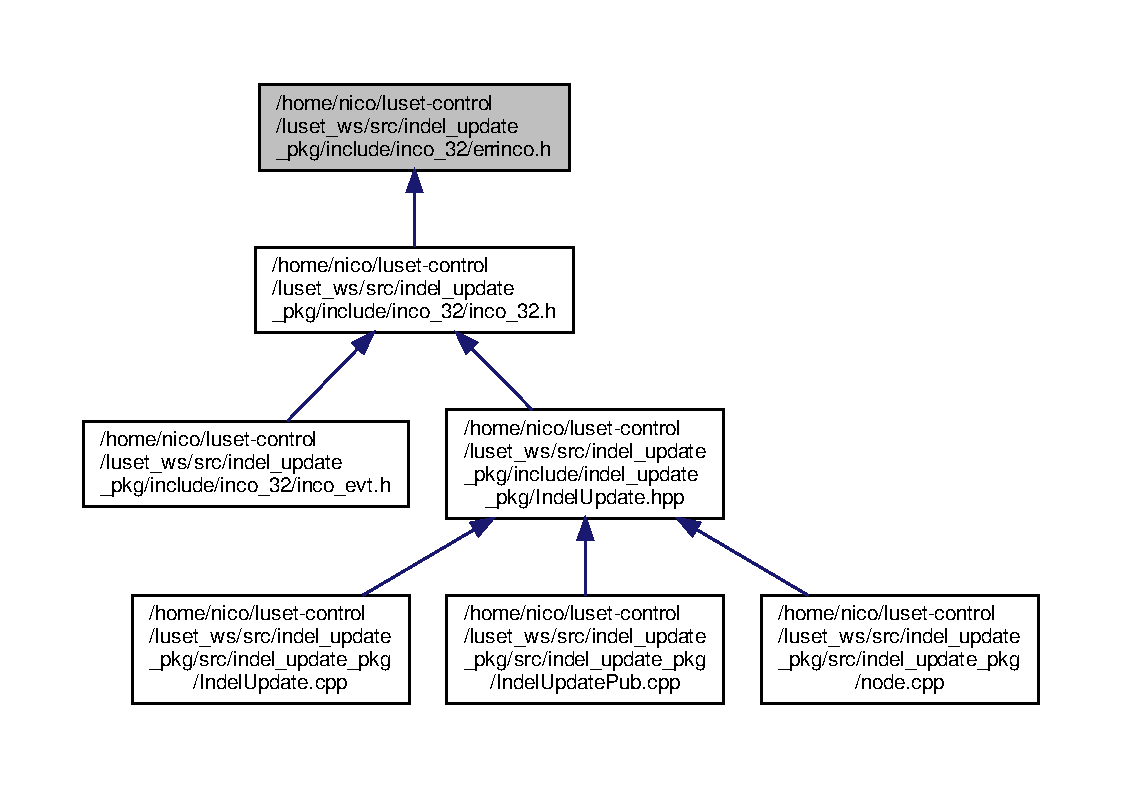
\includegraphics[width=350pt]{errinco_8h__dep__incl}
\end{center}
\end{figure}
\subsection*{Macros}
\begin{Indent}\textbf{ Error ranges}\par
\begin{DoxyCompactItemize}
\item 
\#define \hyperlink{errinco_8h_a272ef6d7861109ac2a23a432debbd717}{E\+R\+\_\+\+A\+P\+P\+E\+R\+R\+O\+R\+\_\+\+B\+A\+SE}~0x40000000
\begin{DoxyCompactList}\small\item\em use this mask to check for an application error defined by the Mc\+Robot framework \end{DoxyCompactList}\item 
\#define \hyperlink{errinco_8h_a7bc1f2dbefeb58d275a525d3c26f4ed2}{E\+R\+\_\+\+A\+P\+P\+E\+R\+R\+O\+R\+\_\+\+C\+U\+S\+T\+O\+M\+ER}~0x80000000
\begin{DoxyCompactList}\small\item\em use this mask to check for an application error defined by customer code \end{DoxyCompactList}\end{DoxyCompactItemize}
\end{Indent}
\begin{Indent}\textbf{ Error range masks}\par
\begin{DoxyCompactItemize}
\item 
\#define \hyperlink{errinco_8h_a365d1bd8b8001bad2568ed7ea79a7bb6}{E\+R\+\_\+\+M\+A\+S\+K\+\_\+\+A\+P\+P\+E\+R\+R\+OR}~0x\+F0\+F\+F\+F\+F\+FF
\begin{DoxyCompactList}\small\item\em use this mask to get the application error value (without the Rpl\+Id) \end{DoxyCompactList}\item 
\#define \hyperlink{errinco_8h_a4989e978ddad311b8cd02dbeb98f0088}{E\+R\+\_\+\+M\+A\+S\+K\+\_\+\+A\+P\+P\+E\+R\+R\+O\+R\+\_\+\+T\+Y\+PE}~0x\+F0000000
\begin{DoxyCompactList}\small\item\em use this mask to check for an application error defined by the Mc\+Robot framework \end{DoxyCompactList}\item 
\#define \hyperlink{errinco_8h_a20402b4ba53dedbf0535d73a27b2d4d5}{E\+R\+\_\+\+M\+A\+S\+K\+\_\+\+A\+P\+P\+L\+I\+C\+A\+T\+I\+O\+N\+\_\+\+R\+P\+L\+\_\+\+ID}~0x0\+F000000
\begin{DoxyCompactList}\small\item\em use this mask to extract the reply id (e.\+g. ok, skip, error, etc.) from the application error \end{DoxyCompactList}\item 
\#define \hyperlink{errinco_8h_add9783c9d3748a01476686d359be3407}{E\+R\+\_\+\+M\+A\+S\+K\+\_\+\+A\+P\+P\+L\+I\+C\+A\+T\+I\+O\+N\+\_\+\+R\+P\+L\+\_\+\+I\+D\+\_\+\+O\+F\+F\+S\+ET}~24
\begin{DoxyCompactList}\small\item\em use this offset to shift the Rpl\+Id to the right when read from an application error, like this\+: u\+Rpl\+Id = (u\+Error \& E\+R\+\_\+\+M\+A\+S\+K\+\_\+\+A\+P\+P\+L\+I\+C\+A\+T\+I\+O\+N\+\_\+\+R\+P\+L\+\_\+\+ID) $>$$>$ E\+R\+\_\+\+M\+A\+S\+K\+\_\+\+A\+P\+P\+L\+I\+C\+A\+T\+I\+O\+N\+\_\+\+R\+P\+L\+\_\+\+I\+D\+\_\+\+O\+F\+F\+S\+ET; \end{DoxyCompactList}\end{DoxyCompactItemize}
\end{Indent}
\begin{Indent}\textbf{ I\+N\+CO errors}\par
\begin{DoxyCompactItemize}
\item 
\#define \hyperlink{errinco_8h_ac806a12a2f08c29e901360403c9e239e}{E\+R\+\_\+\+I\+N\+C\+O\+\_\+\+N\+O\+\_\+\+E\+R\+R\+OR}~0x00000000L
\begin{DoxyCompactList}\small\item\em ok \end{DoxyCompactList}\item 
\#define \hyperlink{errinco_8h_ad0c8ffa42bc2c55afc03fe860c1ac3c0}{E\+R\+\_\+\+I\+N\+C\+O\+\_\+\+D\+E\+P\+R\+E\+C\+A\+T\+ED}~0x00010000L
\begin{DoxyCompactList}\small\item\em deprecated function or functionality \end{DoxyCompactList}\item 
\#define \hyperlink{errinco_8h_a74ecddf0b0fdeaf788eb9eb1a0ab1181}{E\+R\+\_\+\+I\+N\+C\+O\+\_\+\+R\+E\+G\+I\+S\+T\+RY}~0x00010001L
\begin{DoxyCompactList}\small\item\em error in local registry \end{DoxyCompactList}\item 
\#define \hyperlink{errinco_8h_a06b82bb48eb9a17bf498576b18ad8605}{E\+R\+\_\+\+I\+N\+C\+O\+\_\+\+S\+E\+R\+V\+E\+R\+\_\+\+R\+E\+G\+I\+S\+T\+RY}~0x00010002L
\begin{DoxyCompactList}\small\item\em error in server registry \end{DoxyCompactList}\item 
\#define \hyperlink{errinco_8h_a32d7f83b48f4940bdd5aff2e010d71a9}{E\+R\+\_\+\+I\+N\+C\+O\+\_\+\+T\+A\+R\+G\+ET}~0x00010003L
\begin{DoxyCompactList}\small\item\em target not available \end{DoxyCompactList}\item 
\#define \hyperlink{errinco_8h_a48879217022502ae4fb6a3a35af481ac}{E\+R\+\_\+\+I\+N\+C\+O\+\_\+\+M\+A\+S\+T\+E\+R\+\_\+\+N\+A\+ME}~0x00010004L
\begin{DoxyCompactList}\small\item\em master name not available \end{DoxyCompactList}\item 
\#define \hyperlink{errinco_8h_a06dbdc8b480263dd7b91f2a29ee08c96}{E\+R\+\_\+\+I\+N\+C\+O\+\_\+\+T\+I\+M\+E\+O\+UT}~0x00010005L
\begin{DoxyCompactList}\small\item\em no answer from target \end{DoxyCompactList}\item 
\#define \hyperlink{errinco_8h_a5ae0ccc9ebf1a6b72b213728dcfe4a07}{E\+R\+\_\+\+I\+N\+C\+O\+\_\+\+T\+I\+M\+E\+O\+U\+T\+\_\+\+S\+E\+M\+A\+P\+H\+O\+RE}~0x00010006L
\begin{DoxyCompactList}\small\item\em could not reserve semaphore \end{DoxyCompactList}\item 
\#define \hyperlink{errinco_8h_abbd332d22911aad5bc90e928d8472326}{E\+R\+\_\+\+I\+N\+C\+O\+\_\+\+R\+E\+S\+E\+T\+\_\+\+S\+E\+M\+A\+P\+H\+O\+RE}~0x00010007L
\begin{DoxyCompactList}\small\item\em could not reset semaphore \end{DoxyCompactList}\item 
\#define \hyperlink{errinco_8h_a431f5a23584bd527eb030a90e0bc5484}{E\+R\+\_\+\+I\+N\+C\+O\+\_\+\+P\+A\+S\+S\+W\+O\+R\+D\+\_\+\+R\+E\+Q\+U\+I\+R\+ED}~0x00010008L
\begin{DoxyCompactList}\small\item\em password needs to be set \end{DoxyCompactList}\item 
\#define \hyperlink{errinco_8h_a65cd94c28f114a1b4bc2089e144799a2}{E\+R\+\_\+\+I\+N\+C\+O\+\_\+\+S\+T\+R\+I\+N\+G\+\_\+\+T\+O\+O\+\_\+\+L\+O\+NG}~0x00010009L
\begin{DoxyCompactList}\small\item\em string too long for buffer \end{DoxyCompactList}\item 
\#define \hyperlink{errinco_8h_a93fd5ae255df6295af1fdd44e1b80c1c}{E\+R\+\_\+\+I\+N\+C\+O\+\_\+\+N\+O\+\_\+\+F\+U\+N\+C\+T\+I\+ON}~0x00010010L
\begin{DoxyCompactList}\small\item\em function not defined \end{DoxyCompactList}\item 
\#define \hyperlink{errinco_8h_a361ca6524fd512143ac9412a185054cf}{E\+R\+\_\+\+I\+N\+C\+O\+\_\+\+M\+E\+M\+\_\+\+D\+R\+I\+V\+ER}~0x00010011L
\begin{DoxyCompactList}\small\item\em server could not load memdriver \end{DoxyCompactList}\item 
\#define \hyperlink{errinco_8h_a98e02cc83f137daf981a246f7ce09ec7}{E\+R\+\_\+\+I\+N\+C\+O\+\_\+\+T\+I\+M\+O\+U\+T\+\_\+\+F\+R\+A\+ME}~0x00010012L
\begin{DoxyCompactList}\small\item\em timeout while waiting for incoframe \end{DoxyCompactList}\item 
\#define \hyperlink{errinco_8h_a6d39ecff4db39bd4d4a79973a63401cb}{E\+R\+\_\+\+I\+N\+C\+O\+\_\+\+D\+P\+R\+\_\+\+W\+R\+I\+TE}~0x00010013L
\begin{DoxyCompactList}\small\item\em write error in dual-\/port or no target \end{DoxyCompactList}\item 
\#define \hyperlink{errinco_8h_a56e9c5f5ff6ce06e9d2394ea25e74cff}{E\+R\+\_\+\+I\+N\+C\+O\+\_\+\+B\+O\+O\+T\+\_\+\+C\+O\+DE}~0x00010014L
\begin{DoxyCompactList}\small\item\em boot code for target not found \end{DoxyCompactList}\item 
\#define \hyperlink{errinco_8h_ad18a4ada1b5182fc8eec84787dc25efe}{E\+R\+\_\+\+I\+N\+C\+O\+\_\+\+O\+N\+L\+Y\+\_\+\+N\+U\+M\+B\+E\+RS}~0x00010016L
\begin{DoxyCompactList}\small\item\em only numbers supported (no names) \end{DoxyCompactList}\item 
\#define \hyperlink{errinco_8h_ad0547946e0606e26b5b822b8d5b9627f}{E\+R\+\_\+\+I\+N\+C\+O\+\_\+\+N\+O\+\_\+\+P\+P\+C\+\_\+\+A\+T\+\_\+\+A\+D\+D\+R\+E\+SS}~0x00010017L
\begin{DoxyCompactList}\small\item\em no P\+PC found at given address \end{DoxyCompactList}\item 
\#define \hyperlink{errinco_8h_a3bb81fcb323f2e5a05dc86be917a3afc}{E\+R\+\_\+\+I\+N\+C\+O\+\_\+\+P\+L\+X\+\_\+\+O\+P\+E\+N\+\_\+\+F\+A\+I\+L\+ED}~0x00010018L
\begin{DoxyCompactList}\small\item\em The Plx api wasn\textquotesingle{}t able to open the device at specified bus/slot. \end{DoxyCompactList}\item 
\#define \hyperlink{errinco_8h_a7ce027d6e977494df750a174709322ef}{E\+R\+\_\+\+I\+N\+C\+O\+\_\+\+S\+E\+R\+V\+E\+R\+\_\+\+T\+O\+O\+\_\+\+O\+LD}~0x00010020L
\begin{DoxyCompactList}\small\item\em Inco\+Server too old for this functionality. \end{DoxyCompactList}\item 
\#define \hyperlink{errinco_8h_a7dd67eee1f0fd12b13abba67fdc84ab2}{E\+R\+\_\+\+I\+N\+C\+O\+\_\+\+T\+I\+M\+E\+O\+U\+T\+\_\+\+F\+R\+A\+M\+E\+\_\+\+T\+CP}~0x00010021L
\begin{DoxyCompactList}\small\item\em timeout while waiting for incoframe in libinco\+\_\+32 using Tcp/\+Ip \end{DoxyCompactList}\item 
\#define \hyperlink{errinco_8h_a9990c3a3d0e4d44f3355933466d8976b}{E\+R\+\_\+\+I\+N\+C\+O\+\_\+\+T\+I\+M\+E\+O\+U\+T\+\_\+\+T\+A\+R\+G\+E\+T\+\_\+\+S\+E\+R\+I\+A\+L\+I\+Z\+ER}~0x00010022L
\begin{DoxyCompactList}\small\item\em Timeout while waiting to get exclusive access to the target communication port (within I\+N\+C\+O\+Server) \end{DoxyCompactList}\item 
\#define \hyperlink{errinco_8h_a3b4f32933f59bfe3fd28e8948a481772}{E\+R\+\_\+\+I\+N\+C\+O\+\_\+\+T\+A\+R\+G\+E\+T\+\_\+\+C\+O\+U\+N\+T\+\_\+\+E\+X\+C\+E\+E\+D\+ED}~0x00010030L
\begin{DoxyCompactList}\small\item\em Maximum count of target-\/subtarget reached. The amount of subtargets is limited. \end{DoxyCompactList}\item 
\#define \hyperlink{errinco_8h_a84d7ac962aff105f6f5a63bd14d94191}{E\+R\+\_\+\+I\+N\+C\+O\+\_\+\+T\+A\+R\+G\+E\+T\+\_\+\+P\+O\+R\+T\+\_\+\+I\+N\+V\+A\+L\+ID}~0x00010031L
\begin{DoxyCompactList}\small\item\em Invalid target name passed to inco function. \end{DoxyCompactList}\item 
\#define \hyperlink{errinco_8h_a83b3d7633020c2ecbae0633cee13b64c}{E\+R\+\_\+\+I\+N\+C\+O\+\_\+\+T\+A\+R\+G\+E\+T\+\_\+\+N\+A\+M\+E\+\_\+\+I\+N\+V\+A\+L\+ID}~0x00010032L
\begin{DoxyCompactList}\small\item\em Invalid target name passed to inco function. \end{DoxyCompactList}\item 
\#define \hyperlink{errinco_8h_a0829b1a257d431848013a427895e83da}{E\+R\+\_\+\+I\+N\+C\+O\+\_\+\+T\+A\+R\+G\+E\+T\+\_\+\+A\+L\+R\+E\+A\+D\+Y\+\_\+\+E\+X\+I\+S\+TS}~0x00010033L
\begin{DoxyCompactList}\small\item\em a target with this name already exists. \end{DoxyCompactList}\item 
\#define \hyperlink{errinco_8h_ab44d0168aff4a82dd86a387db33a51db}{E\+R\+\_\+\+I\+N\+C\+O\+\_\+\+T\+A\+R\+G\+E\+T\+A\+L\+I\+A\+S\+\_\+\+N\+A\+ME}~0x00010034L
\begin{DoxyCompactList}\small\item\em No target alias with that name exists. \end{DoxyCompactList}\item 
\#define \hyperlink{errinco_8h_a1932cd726d21e4347b3b72912299948a}{E\+R\+\_\+\+I\+N\+C\+O\+\_\+\+T\+A\+R\+G\+E\+T\+A\+L\+I\+A\+S\+\_\+\+A\+L\+R\+E\+A\+D\+Y\+\_\+\+E\+X\+I\+S\+TS}~0x00010035L
\begin{DoxyCompactList}\small\item\em a target alias with this name already exists. \end{DoxyCompactList}\item 
\#define \hyperlink{errinco_8h_ab57a823f0c2222c4ec9ccf697a174c9f}{E\+R\+\_\+\+I\+N\+C\+O\+\_\+\+F\+R\+A\+G\+M\+E\+N\+T\+A\+T\+I\+O\+N\+\_\+\+U\+N\+S\+U\+P\+P\+O\+R\+T\+ED}~0x00010036L
\begin{DoxyCompactList}\small\item\em Fragmented I\+N\+CO frames are not supported by this target/server. \end{DoxyCompactList}\item 
\#define \hyperlink{errinco_8h_a4a37c1d4c02fdefff867d777470af91b}{E\+R\+\_\+\+I\+N\+C\+O\+\_\+\+S\+E\+R\+V\+E\+R4\+\_\+\+N\+O\+T\+\_\+\+R\+U\+N\+N\+I\+NG}~0x00010040L
\begin{DoxyCompactList}\small\item\em incoserver 4.\+x is not running. Connection failed. \end{DoxyCompactList}\item 
\#define \hyperlink{errinco_8h_ad84abb2b045cb2b2d604e04709a99adf}{E\+R\+\_\+\+I\+N\+C\+O\+\_\+\+F\+R\+A\+M\+E\+\_\+\+B\+U\+F\+F\+E\+R\+\_\+\+F\+U\+LL}~0x00010050L
\begin{DoxyCompactList}\small\item\em the frame buffer is full -\/ therfore the frame couldn\textquotesingle{}t be processed. \end{DoxyCompactList}\item 
\#define \hyperlink{errinco_8h_aa3ddfafed55ca354ff6988148f1332dd}{E\+R\+\_\+\+I\+N\+C\+O\+\_\+\+F\+R\+A\+M\+E\+\_\+\+C\+O\+N\+V\+E\+R\+S\+I\+O\+N\+\_\+\+B\+U\+F\+F\+ER}~0x00010051L
\begin{DoxyCompactList}\small\item\em The inco frame conversion failed because the frame buffer of the classic frame is too small. \end{DoxyCompactList}\item 
\#define \hyperlink{errinco_8h_a6712ee16c444831c5ef251890ba7a8f1}{E\+R\+\_\+\+I\+N\+C\+O\+\_\+\+F\+R\+A\+M\+E\+\_\+\+D\+A\+T\+A\+\_\+\+S\+I\+Z\+E\+\_\+\+T\+O\+O\+\_\+\+S\+M\+A\+LL}~0x00010052L
\begin{DoxyCompactList}\small\item\em The data size of the inco frame is not big enough to perform the operation. \end{DoxyCompactList}\item 
\#define \hyperlink{errinco_8h_a825b7529f69a64e95977df1c2a92c322}{E\+R\+\_\+\+I\+N\+C\+O\+\_\+\+F\+R\+A\+M\+E\+\_\+\+F\+R\+A\+G\+M\+E\+N\+T\+E\+D\+\_\+\+S\+I\+Z\+E\+\_\+\+T\+O\+O\+\_\+\+S\+M\+A\+LL}~0x00010053L
\begin{DoxyCompactList}\small\item\em The data size exceeds the maximum possible data size of fragmented frames. \end{DoxyCompactList}\item 
\#define \hyperlink{errinco_8h_a17b27da1a04577974b98ebbfcae42d31}{E\+R\+\_\+\+I\+N\+C\+O\+\_\+\+F\+R\+A\+M\+E\+\_\+\+F\+R\+A\+G\+M\+E\+N\+T\+E\+D\+\_\+\+D\+O\+E\+S\+N\+T\+\_\+\+M\+A\+T\+CH}~0x00010054L
\begin{DoxyCompactList}\small\item\em The two frames are not from the same fragmented I\+N\+CO frame. \end{DoxyCompactList}\item 
\#define \hyperlink{errinco_8h_a1dfd9d41caa54c368c02d53714c446fa}{E\+R\+\_\+\+I\+N\+C\+O\+\_\+\+F\+R\+A\+M\+E\+\_\+\+F\+R\+A\+G\+M\+E\+N\+T\+E\+D\+\_\+\+M\+A\+X\+\_\+\+S\+I\+ZE}~0x00010055L
\begin{DoxyCompactList}\small\item\em The receiving target can\textquotesingle{}t handle that big fragmented frames. \end{DoxyCompactList}\item 
\#define \hyperlink{errinco_8h_a1507ea7594a13dd875686eda0b772849}{E\+R\+\_\+\+I\+N\+C\+O\+\_\+\+C\+T\+L\+\_\+\+U\+N\+K\+N\+O\+W\+N\+\_\+\+R\+E\+Q\+U\+E\+ST}~0x00010100L
\begin{DoxyCompactList}\small\item\em Unknown request to \hyperlink{inco__32_8h_a106f32a0a06c9d0ac790ab66f8554ca0}{Inco\+Control}. \end{DoxyCompactList}\item 
\#define \hyperlink{errinco_8h_a9f3eff1f143750ab3e168d26875cabc4}{E\+R\+\_\+\+T\+A\+R\+G\+E\+T\+\_\+\+S\+I\+O\+\_\+\+P\+O\+R\+T\+\_\+\+R\+A\+N\+GE}~0x00020000L
\begin{DoxyCompactList}\small\item\em the comport is out of range \end{DoxyCompactList}\item 
\#define \hyperlink{errinco_8h_a9ba064a3d08b70c00897a7cbf5c85313}{E\+R\+\_\+\+T\+A\+R\+G\+E\+T\+\_\+\+S\+I\+O\+\_\+\+P\+O\+R\+T\+\_\+\+I\+N\+\_\+\+U\+SE}~0x00020001L
\begin{DoxyCompactList}\small\item\em the comport is already used by an other target \end{DoxyCompactList}\item 
\#define \hyperlink{errinco_8h_aef4fdc8d2d6e5acb26f07010a269f3ae}{E\+R\+\_\+\+T\+A\+R\+G\+E\+T\+\_\+\+S\+I\+O\+\_\+\+S\+E\+N\+D\+\_\+\+F\+A\+I\+L\+ED}~0x00020002L
\begin{DoxyCompactList}\small\item\em the data couldn\textquotesingle{}t be written to the sio port \end{DoxyCompactList}\item 
\#define \hyperlink{errinco_8h_a58f7ce61311c956bcd5148c8818ba7b6}{E\+R\+\_\+\+T\+A\+R\+G\+E\+T\+\_\+\+S\+I\+O\+\_\+\+D\+I\+S\+A\+B\+L\+ED}~0x00020003L
\begin{DoxyCompactList}\small\item\em the sio port is currently disabled \end{DoxyCompactList}\item 
\#define \hyperlink{errinco_8h_ae0bd296796eee768d29704cb0b887950}{E\+R\+\_\+\+T\+A\+R\+G\+E\+T\+\_\+\+S\+I\+O\+\_\+\+O\+P\+E\+N\+\_\+\+F\+A\+I\+L\+ED}~0x00020004L
\begin{DoxyCompactList}\small\item\em opening the comport failed \end{DoxyCompactList}\item 
\#define \hyperlink{errinco_8h_a6aac05ece201fbf81633462dbb15327f}{E\+R\+\_\+\+T\+A\+R\+G\+E\+T\+\_\+\+N\+E\+T\+\_\+\+S\+E\+N\+D\+\_\+\+F\+A\+I\+L\+ED}~0x00020010L
\begin{DoxyCompactList}\small\item\em sending the U\+DP frame to the target failed. \end{DoxyCompactList}\item 
\#define \hyperlink{errinco_8h_ad85e31ffdcfb1fa7b8070646c9c9f561}{E\+R\+\_\+\+T\+A\+R\+G\+E\+T\+\_\+\+N\+E\+T\+\_\+\+M\+A\+L\+F\+O\+R\+M\+E\+D\+\_\+\+IP}~0x00020011L
\begin{DoxyCompactList}\small\item\em the target ip address is malformed. \end{DoxyCompactList}\item 
\#define \hyperlink{errinco_8h_acb6ac23e47a5bacdf22e116f2dc25776}{E\+R\+\_\+\+T\+A\+R\+G\+E\+T\+\_\+\+N\+E\+T\+\_\+\+I\+P\+\_\+\+A\+L\+R\+E\+A\+D\+Y\+\_\+\+I\+N\+\_\+\+U\+SE}~0x00020012L
\begin{DoxyCompactList}\small\item\em the target ip address is already in use by another network target. \end{DoxyCompactList}\item 
\#define \hyperlink{errinco_8h_ab7eac3fc960e74d80e61339304a73814}{E\+R\+\_\+\+T\+A\+R\+G\+E\+T\+\_\+\+N\+E\+T\+\_\+\+N\+O\+\_\+\+N\+E\+T\+W\+O\+R\+K\+\_\+\+F\+O\+R\+\_\+\+T\+A\+R\+G\+ET}~0x00020013L
\begin{DoxyCompactList}\small\item\em no network card could be found with a suitable IP range to reach the target. \end{DoxyCompactList}\item 
\#define \hyperlink{errinco_8h_a58efaea93925dd07eaf4cc12e5d974b1}{E\+R\+\_\+\+T\+A\+R\+G\+E\+T\+\_\+\+N\+E\+T\+\_\+\+B\+I\+N\+D\+\_\+\+F\+A\+I\+L\+ED}~0x00020014L
\begin{DoxyCompactList}\small\item\em binding the udp socket to the specific ip/port failed (bind returned an error). \end{DoxyCompactList}\item 
\#define \hyperlink{errinco_8h_a7634d66082e95c28e7efeb965eed2af6}{E\+R\+\_\+\+T\+A\+R\+G\+E\+T\+\_\+\+N\+E\+T\+\_\+\+R\+E\+C\+V\+\_\+\+F\+A\+I\+L\+ED}~0x00020015L
\begin{DoxyCompactList}\small\item\em receiving the U\+DP frame from the target failed. \end{DoxyCompactList}\item 
\#define \hyperlink{errinco_8h_a6276c6ab0b61b785206ccecee47ac27e}{E\+R\+\_\+\+T\+A\+R\+G\+E\+T\+\_\+\+N\+E\+T\+\_\+\+P\+O\+R\+T\+\_\+\+U\+N\+R\+E\+A\+C\+H\+A\+B\+LE}~0x00020016L
\begin{DoxyCompactList}\small\item\em target U\+DP port unreachable (nobody listening on port 1964?) \end{DoxyCompactList}\item 
\#define \hyperlink{errinco_8h_a00570d5d3984430559b92e880718ad90}{E\+R\+\_\+\+T\+A\+R\+G\+E\+T\+\_\+\+R\+E\+M\+O\+T\+E\+\_\+\+N\+O\+\_\+\+S\+O\+C\+K\+ET}~0x00020020L
\begin{DoxyCompactList}\small\item\em socket for remote target couldn\textquotesingle{}t be found \end{DoxyCompactList}\item 
\#define \hyperlink{errinco_8h_a72cd302e042abe8c4140eb65c61d9f9f}{E\+R\+\_\+\+T\+A\+R\+G\+E\+T\+\_\+\+R\+E\+M\+O\+T\+E\+\_\+\+S\+E\+N\+D\+\_\+\+F\+A\+I\+L\+ED}~0x00020021L
\begin{DoxyCompactList}\small\item\em sending data to remote server failed. \end{DoxyCompactList}\item 
\#define \hyperlink{errinco_8h_a01b90f1b578de66ef1b518fc1a6e9c4e}{E\+R\+\_\+\+T\+A\+R\+G\+E\+T\+\_\+\+R\+E\+C\+E\+I\+V\+E\+\_\+\+F\+A\+I\+L\+ED}~0x00020022L
\begin{DoxyCompactList}\small\item\em receiving data from remote server failed. \end{DoxyCompactList}\item 
\#define \hyperlink{errinco_8h_ab8ae8f462b424eda645e127a5b1c0337}{E\+R\+\_\+\+T\+A\+R\+G\+E\+T\+\_\+\+R\+E\+M\+O\+T\+E\+\_\+\+C\+O\+N\+N\+E\+C\+T\+E\+D\+\_\+\+S\+R\+V\+\_\+\+G\+O\+NE}~0\+X00020023L
\begin{DoxyCompactList}\small\item\em a remote server that was connected to this server has gone \end{DoxyCompactList}\item 
\#define \hyperlink{errinco_8h_a9c3f72a26b08eb2f71643e4f0da46aa2}{E\+R\+\_\+\+T\+A\+R\+G\+E\+T\+\_\+\+R\+E\+M\+O\+T\+E\+\_\+\+S\+R\+V\+\_\+\+N\+O\+T\+\_\+\+F\+O\+U\+ND}~0x00020024L
\begin{DoxyCompactList}\small\item\em the remote server name or IP could not be resolved \end{DoxyCompactList}\item 
\#define \hyperlink{errinco_8h_af517b2b395c600aa22ae235ce3f44bea}{E\+R\+\_\+\+T\+A\+R\+G\+E\+T\+\_\+\+R\+E\+M\+O\+T\+E\+\_\+\+S\+R\+V\+\_\+\+C\+O\+N\+N\+E\+C\+T\+I\+N\+G\+\_\+\+F\+A\+I\+L\+ED}~0x00020025L
\begin{DoxyCompactList}\small\item\em connecting to the remote server failed. Maybe server not running? \end{DoxyCompactList}\item 
\#define \hyperlink{errinco_8h_adf3006e1e4a72cdc8b6b3c4037e9ad3e}{E\+R\+\_\+\+T\+A\+R\+G\+E\+T\+\_\+\+R\+E\+M\+O\+T\+E\+\_\+\+S\+R\+V\+\_\+\+C\+O\+N\+N\+E\+C\+T\+I\+N\+G\+\_\+\+T\+I\+M\+E\+D\+O\+UT}~0x00020026L
\begin{DoxyCompactList}\small\item\em Connecting to the remote server failed\+: Time out. Maybe server not running? \end{DoxyCompactList}\item 
\#define \hyperlink{errinco_8h_ad82f5e9af7294a6060fc2df5da6485e7}{E\+R\+\_\+\+T\+A\+R\+G\+E\+T\+\_\+\+R\+E\+M\+O\+T\+E\+\_\+\+S\+R\+V\+\_\+\+C\+O\+N\+N\+E\+C\+T\+I\+N\+G\+\_\+\+S\+O\+C\+K\+O\+P\+T\+\_\+\+F\+A\+I\+L\+ED}~0x00020027L
\begin{DoxyCompactList}\small\item\em Connecting to the remote server failed\+: getsockopt returned an error. Maybe server not running? \end{DoxyCompactList}\item 
\#define \hyperlink{errinco_8h_a582a0df20119fe320239a714f6203102}{E\+R\+\_\+\+T\+A\+R\+G\+E\+T\+\_\+\+R\+E\+M\+O\+T\+E\+\_\+\+S\+R\+V\+\_\+\+C\+O\+N\+N\+E\+C\+T\+I\+N\+G\+\_\+\+W\+R\+O\+N\+G\+\_\+\+S\+E\+L\+E\+CT}~0x00020028L
\begin{DoxyCompactList}\small\item\em Connecting to the remote server failed. select returned wrong set. Maybe server not running? \end{DoxyCompactList}\item 
\#define \hyperlink{errinco_8h_a1f01c8b471c788de983e26864a25fcf6}{E\+R\+\_\+\+T\+A\+R\+G\+E\+T\+\_\+\+R\+E\+M\+O\+T\+E\+\_\+\+S\+R\+V\+\_\+\+C\+O\+N\+N\+E\+C\+T\+I\+N\+G\+\_\+\+N\+O\+B\+L\+O\+CK}~0x00020029L
\begin{DoxyCompactList}\small\item\em Connecting to the remote server failed. connect didn\textquotesingle{}t return \textquotesingle{}wouldblock\textquotesingle{}. Maybe server not running? \end{DoxyCompactList}\item 
\#define \hyperlink{errinco_8h_a1fec7b34c381230e96a918da963d196f}{E\+R\+\_\+\+T\+A\+R\+G\+E\+T\+\_\+\+R\+E\+M\+O\+T\+E\+\_\+\+S\+R\+V\+\_\+\+C\+O\+N\+N\+E\+C\+T\+I\+N\+G\+\_\+\+C\+O\+N\+N\+E\+C\+T\+\_\+\+F\+A\+I\+L\+ED}~0x0002002\+AL
\begin{DoxyCompactList}\small\item\em Connecting to the remote server failed. connect returned error. Maybe server not running? \end{DoxyCompactList}\item 
\#define \hyperlink{errinco_8h_ad6a47bda58efe2558c05e1c7dba7fed2}{E\+R\+\_\+\+T\+A\+R\+G\+E\+T\+\_\+\+R\+E\+M\+O\+T\+E\+\_\+\+C\+O\+N\+N\+E\+C\+T\+I\+O\+N\+\_\+\+S\+H\+U\+T\+D\+O\+WN}~0\+X0002002\+BL
\begin{DoxyCompactList}\small\item\em the Tcp/\+Ip connection was gracefully shutdown by the remote peer \end{DoxyCompactList}\item 
\#define \hyperlink{errinco_8h_a2648d4abae750262d526b3970ecb7cb0}{E\+R\+\_\+\+T\+A\+R\+G\+E\+T\+\_\+\+R\+E\+M\+O\+T\+E\+\_\+\+S\+E\+L\+E\+C\+T\+\_\+\+F\+A\+I\+L\+ED}~0\+X0002002\+CL
\begin{DoxyCompactList}\small\item\em The Tcp/\+Ip connection could not be established, select() returned an invalid result. \end{DoxyCompactList}\item 
\#define \hyperlink{errinco_8h_afc800eb302ba66588068904dfa8ed00e}{E\+R\+\_\+\+T\+A\+R\+G\+E\+T\+\_\+\+R\+E\+M\+O\+T\+E\+\_\+\+C\+O\+N\+N\+E\+C\+T\+\_\+\+F\+A\+I\+L\+ED}~0\+X0002002\+DL
\begin{DoxyCompactList}\small\item\em The Tcp/\+Ip connection could not be established, connect() returned an error. \end{DoxyCompactList}\item 
\#define \hyperlink{errinco_8h_a72095164b8ae6c7d7a95a948b4b008ca}{E\+R\+\_\+\+T\+A\+R\+G\+E\+T\+\_\+\+R\+E\+M\+O\+T\+E\+\_\+\+C\+O\+N\+N\+E\+C\+T\+\_\+\+N\+O\+T\+\_\+\+E\+I\+N\+P\+R\+O\+G\+R\+E\+SS}~0\+X0002002\+EL
\begin{DoxyCompactList}\small\item\em The Tcp/\+Ip connection could not be established, connect() didn\textquotesingle{}t return E\+I\+N\+P\+R\+O\+G\+R\+E\+SS. \end{DoxyCompactList}\item 
\#define \hyperlink{errinco_8h_a7cc86f94ce454cb4394f54910debfc44}{E\+R\+\_\+\+T\+A\+R\+G\+E\+T\+\_\+\+P\+C\+I\+\_\+\+D\+P\+R\+\_\+\+V\+E\+R\+I\+FY}~0x00020030L
\begin{DoxyCompactList}\small\item\em Writing to the D\+PR failed\+: Verifying the value was wrong. \end{DoxyCompactList}\item 
\#define \hyperlink{errinco_8h_a4109e20157c159ddd122639d5880efcb}{E\+R\+\_\+\+T\+A\+R\+G\+E\+T\+\_\+\+P\+C\+I\+\_\+\+N\+O\+\_\+\+B\+O\+A\+R\+D\+\_\+\+A\+T\+\_\+\+B\+U\+S\+\_\+\+S\+L\+OT}~0x00020031L
\begin{DoxyCompactList}\small\item\em No board could be found at configured bus/slot pair. \end{DoxyCompactList}\item 
\#define \hyperlink{errinco_8h_a9de8f47f3fe0812f01c15325d6287a5a}{E\+R\+\_\+\+T\+A\+R\+G\+E\+T\+\_\+\+P\+C\+I\+\_\+\+B\+O\+A\+R\+D\+\_\+\+A\+L\+R\+E\+A\+D\+Y\+\_\+\+U\+S\+ED}~0x00020032L
\begin{DoxyCompactList}\small\item\em The configured board at configured bus/slot is already in use. \end{DoxyCompactList}\item 
\#define \hyperlink{errinco_8h_a7bcae76fc2e6c183cedbca61e00cc183}{E\+R\+\_\+\+T\+A\+R\+G\+E\+T\+\_\+\+P\+C\+I\+\_\+\+P\+L\+X\+B\+A\+R\+M\+A\+P\+\_\+\+F\+A\+I\+L\+ED}~0x00020033L
\begin{DoxyCompactList}\small\item\em Plx\+Bar\+Map returned an error. The P\+CI board can\textquotesingle{}t be opened. \end{DoxyCompactList}\item 
\#define \hyperlink{errinco_8h_ab681fdac1600b4aa7003d95c8cb2fd8d}{E\+R\+\_\+\+T\+A\+R\+G\+E\+T\+\_\+\+P\+C\+I\+\_\+\+R\+E\+A\+D\+\_\+\+E\+E\+P\+R\+O\+M\+\_\+\+F\+A\+I\+L\+ED}~0x00020034L
\begin{DoxyCompactList}\small\item\em Reading the E\+E\+P\+R\+OM of the P\+CI board failed. \end{DoxyCompactList}\item 
\#define \hyperlink{errinco_8h_aba388cdc29f4920bc38f3e0d4f429aa0}{E\+R\+\_\+\+T\+A\+R\+G\+E\+T\+\_\+\+P\+C\+I\+\_\+\+B\+U\+F\+F\+E\+R\+\_\+\+T\+O\+O\+\_\+\+S\+M\+A\+LL}~0x00020035L
\begin{DoxyCompactList}\small\item\em The data length in the D\+PR is longer than the buffer available by the I\+N\+O\+C\+Server. Very strange. \end{DoxyCompactList}\item 
\#define \hyperlink{errinco_8h_abb0f04dac08f8fc15ad7d03fd4b5818b}{E\+R\+\_\+\+T\+A\+R\+G\+E\+T\+\_\+\+P\+C\+I\+\_\+\+B\+O\+O\+T\+C\+O\+D\+E\+\_\+\+R\+E\+A\+D\+\_\+\+F\+A\+I\+L\+ED}~0x00020036L
\begin{DoxyCompactList}\small\item\em Reading the bootcode failed (fread() returned error) \end{DoxyCompactList}\item 
\#define \hyperlink{errinco_8h_a6af19438af0b90072d3e03b3e565f6ab}{E\+R\+\_\+\+T\+A\+R\+G\+E\+T\+\_\+\+P\+C\+I\+\_\+\+G\+I\+N\+P\+C\+I\+E\+\_\+\+R\+E\+S\+E\+T\+\_\+\+F\+A\+I\+L\+ED}~0x00020037L
\begin{DoxyCompactList}\small\item\em The G\+I\+N-\/\+P\+C\+Ie reset failed. \end{DoxyCompactList}\item 
\#define \hyperlink{errinco_8h_add8ae0e5e63664133ef37cb935664fcb}{E\+R\+\_\+\+T\+A\+R\+G\+E\+T\+\_\+\+P\+C\+I\+\_\+1\+S\+T\+\_\+\+S\+T\+A\+G\+E\+\_\+\+U\+B\+O\+O\+T\+\_\+\+N\+O\+T\+\_\+\+R\+UN}~0x00020038L
\begin{DoxyCompactList}\small\item\em The G\+I\+N-\/\+P\+C\+Ie 1st stage u-\/boot seems to be not running. \end{DoxyCompactList}\item 
\#define \hyperlink{errinco_8h_af1bcd00af665ebe93732e61457d90537}{E\+R\+\_\+\+T\+A\+R\+G\+E\+T\+\_\+\+P\+C\+I\+\_\+\+I\+N\+O\+S\+\_\+\+B\+O\+O\+T\+L\+O\+A\+D\+E\+R\+\_\+\+N\+O\+T\+\_\+\+R\+UN}~0x00020039L
\begin{DoxyCompactList}\small\item\em The G\+I\+N-\/\+P\+C\+Ie I\+N\+OS bootloader seems to be not running. \end{DoxyCompactList}\item 
\#define \hyperlink{errinco_8h_ac1144afaf9404081f8c940a272092951}{E\+R\+\_\+\+T\+A\+R\+G\+E\+T\+\_\+\+P\+C\+I\+\_\+\+N\+O\+T\+\_\+\+Y\+E\+T\+\_\+\+O\+P\+E\+N\+ED}~0x0002003\+AL
\begin{DoxyCompactList}\small\item\em The P\+C\+Master has not yet been opened. \end{DoxyCompactList}\item 
\#define \hyperlink{errinco_8h_a6d5b15c46aece164bc4e0ca1ebeaa2e4}{E\+R\+\_\+\+T\+A\+R\+G\+E\+T\+\_\+\+P\+C\+I\+\_\+\+I\+R\+Q\+\_\+\+U\+N\+S\+U\+P\+P\+O\+R\+T\+ED}~0x0002003\+BL
\begin{DoxyCompactList}\small\item\em The P\+C\+Master does not support interrupts (e.\+g. \char`\"{}\+I\+S\+A compatibility\char`\"{} flag set) \end{DoxyCompactList}\item 
\#define \hyperlink{errinco_8h_a9293965755d583bc68d05835f18dc9fe}{E\+R\+\_\+\+T\+A\+R\+G\+E\+T\+\_\+\+P\+C\+I\+\_\+\+V\+E\+R\+S\+I\+O\+N\+\_\+\+M\+I\+S\+M\+A\+T\+CH}~0x0002003\+CL
\begin{DoxyCompactList}\small\item\em The P\+C\+Master is not compatible to the device driver. Maybe outdated G\+I\+N-\/\+P\+C\+Ie driver? \end{DoxyCompactList}\item 
\#define \hyperlink{errinco_8h_ac8c86ea6f137381cb61a5a26030966a2}{E\+R\+\_\+\+T\+A\+R\+G\+E\+T\+\_\+\+P\+C\+I\+\_\+\+W\+R\+O\+N\+G\+\_\+\+B\+O\+A\+R\+D\+\_\+\+T\+Y\+PE}~0x0002003\+DL
\begin{DoxyCompactList}\small\item\em The Indel P\+CI board is of the wrong type (e.\+g. G\+I\+N-\/\+P\+C\+Ie instead of P\+C\+I2) \end{DoxyCompactList}\item 
\#define \hyperlink{errinco_8h_aa768eb0e8e09d583f376c75d53bbd8ac}{E\+R\+\_\+\+T\+A\+R\+G\+E\+T\+\_\+\+P\+L\+X\+\_\+\+N\+T\+F\+Y\+\_\+\+W\+A\+I\+T\+\_\+\+H\+A\+N\+D\+LE}~0x00020040L
\begin{DoxyCompactList}\small\item\em Plx\+Pci\+\_\+\+Notification\+Wait return \textquotesingle{}invalid handle\textquotesingle{} error. \end{DoxyCompactList}\item 
\#define \hyperlink{errinco_8h_a561a821261e0fb17df5ac2f42c5fcd6a}{E\+R\+\_\+\+T\+A\+R\+G\+E\+T\+\_\+\+P\+L\+X\+\_\+\+N\+T\+F\+Y\+\_\+\+W\+A\+I\+T\+\_\+\+T\+I\+M\+E\+O\+UT}~0x00020041L
\begin{DoxyCompactList}\small\item\em Plx\+Pci\+\_\+\+Notification\+Wait return \textquotesingle{}timeout\textquotesingle{} error. \end{DoxyCompactList}\item 
\#define \hyperlink{errinco_8h_a5781932e0a9a72bf6623028849faf4d3}{E\+R\+\_\+\+T\+A\+R\+G\+E\+T\+\_\+\+P\+L\+X\+\_\+\+N\+T\+F\+Y\+\_\+\+W\+A\+I\+T\+\_\+\+C\+A\+N\+C\+E\+L\+ED}~0x00020042L
\begin{DoxyCompactList}\small\item\em Plx\+Pci\+\_\+\+Notification\+Wait return \textquotesingle{}canceled\textquotesingle{} error. \end{DoxyCompactList}\item 
\#define \hyperlink{errinco_8h_a85f9d31589927cb2f0380672c0cccd29}{E\+R\+\_\+\+T\+A\+R\+G\+E\+T\+\_\+\+P\+L\+X\+\_\+\+N\+T\+F\+Y\+\_\+\+W\+A\+I\+T\+\_\+\+G\+E\+N\+E\+R\+IC}~0x00020043L
\begin{DoxyCompactList}\small\item\em Plx\+Pci\+\_\+\+Notification\+Wait return a not further specified error. \end{DoxyCompactList}\item 
\#define \hyperlink{errinco_8h_a55b9c019130611eab53f6bf3983eab2d}{E\+R\+\_\+\+T\+A\+R\+G\+E\+T\+\_\+\+P\+L\+X\+\_\+\+N\+T\+F\+Y\+\_\+\+R\+E\+G\+\_\+\+G\+E\+N\+E\+R\+IC}~0x00020044L
\begin{DoxyCompactList}\small\item\em Plx\+Pci\+\_\+\+Notification\+Register\+For return a not further specified error. \end{DoxyCompactList}\item 
\#define \hyperlink{errinco_8h_ad51f5980bf3c40d314822e84efd6d2c2}{E\+R\+\_\+\+T\+A\+R\+G\+E\+T\+\_\+\+P\+C\+I\+\_\+\+D\+C\+\_\+\+A\+P\+P\+\_\+\+E\+R\+R\+OR}~0x00020050L
\begin{DoxyCompactList}\small\item\em P\+CI datachannel received an application error. \end{DoxyCompactList}\item 
\#define \hyperlink{errinco_8h_a46c5539a2244b5c1eec0d1ba87f5c39d}{E\+R\+\_\+\+T\+A\+R\+G\+E\+T\+\_\+\+P\+C\+I\+\_\+\+D\+C\+\_\+\+B\+U\+F\+\_\+\+T\+O\+\_\+\+S\+M\+A\+LL}~0x00020051L
\begin{DoxyCompactList}\small\item\em P\+CI datachannel receive data failed because the buffer is too small. \end{DoxyCompactList}\item 
\#define \hyperlink{errinco_8h_aec90634a91c8f1a062c323f727717dea}{E\+R\+\_\+\+T\+A\+R\+G\+E\+T\+\_\+\+P\+C\+I\+\_\+\+D\+C\+\_\+\+S\+P\+U\+R\+I\+O\+U\+S\+\_\+\+I\+RQ}~0x00020052L
\begin{DoxyCompactList}\small\item\em P\+CI datachannel received interrupt but not valid data were available. \end{DoxyCompactList}\item 
\#define \hyperlink{errinco_8h_aa4a8e100d3767804423eec914e887285}{E\+R\+\_\+\+T\+A\+R\+G\+E\+T\+\_\+\+P\+C\+I\+\_\+\+D\+C\+\_\+\+R\+E\+C\+E\+I\+V\+E\+R\+\_\+\+W\+R\+O\+N\+G\+\_\+\+ID}~0x00020053L
\begin{DoxyCompactList}\small\item\em P\+CI datachannel sending data failed because the receiver read wrong data (wrong unique id) \end{DoxyCompactList}\item 
\#define \hyperlink{errinco_8h_a7b17b04609e0f9a8086dbba52f4e85f1}{E\+R\+\_\+\+T\+A\+R\+G\+E\+T\+\_\+\+P\+C\+I\+\_\+\+D\+C\+\_\+\+C\+H\+E\+C\+K\+U\+S\+M\+\_\+\+F\+A\+I\+L\+U\+RE}~0x00020054L
\begin{DoxyCompactList}\small\item\em P\+CI datachannel received data with wrong checksum. \end{DoxyCompactList}\item 
\#define \hyperlink{errinco_8h_a0d556e4a8f557535107b2a106f5df4f8}{E\+R\+\_\+\+T\+A\+R\+G\+E\+T\+\_\+\+A\+U\+T\+O\+S\+C\+A\+N\+\_\+\+T\+A\+R\+G\+E\+T\+\_\+\+N\+A\+M\+E\+\_\+\+E\+X\+I\+S\+TS}~0x000200\+F0L
\begin{DoxyCompactList}\small\item\em a target with the same name as the autoscanned target already exists. \end{DoxyCompactList}\item 
\#define \hyperlink{errinco_8h_acc380ca13e77c8499ff881e0713c3685}{E\+R\+\_\+\+T\+A\+R\+G\+E\+T\+\_\+\+A\+U\+T\+O\+S\+C\+A\+N\+\_\+\+S\+O\+C\+K\+E\+T\+\_\+\+O\+P\+E\+N\+\_\+\+F\+A\+I\+L\+ED}~0x000200\+F1L
\begin{DoxyCompactList}\small\item\em creating a socket failed. \end{DoxyCompactList}\item 
\#define \hyperlink{errinco_8h_a31daaf83d9c9a2988137ceb82570b4c1}{E\+R\+\_\+\+T\+A\+R\+G\+E\+T\+\_\+\+A\+U\+T\+O\+S\+C\+A\+N\+\_\+\+S\+O\+C\+K\+E\+T\+\_\+\+B\+I\+N\+D\+\_\+\+F\+A\+I\+L\+ED}~0x000200\+F2L
\begin{DoxyCompactList}\small\item\em binding the socket failed. \end{DoxyCompactList}\item 
\#define \hyperlink{errinco_8h_ab360089bc112923d826012fb3f45760b}{E\+R\+\_\+\+T\+A\+R\+G\+E\+T\+\_\+\+A\+U\+T\+O\+S\+C\+A\+N\+\_\+\+N\+E\+T\+\_\+\+S\+E\+N\+D\+T\+O\+\_\+\+F\+A\+I\+L\+ED}~0x000200\+F3L
\begin{DoxyCompactList}\small\item\em sendto function returned failure \end{DoxyCompactList}\item 
\#define \hyperlink{errinco_8h_a409057edd19e1857fe7517ee2a137096}{E\+R\+\_\+\+T\+A\+R\+G\+E\+T\+\_\+\+U\+R\+L\+\_\+\+M\+I\+S\+S\+I\+N\+G\+\_\+\+U\+RL}~0x00021000L
\begin{DoxyCompactList}\small\item\em no target U\+RL specified \end{DoxyCompactList}\item 
\#define \hyperlink{errinco_8h_ae05d86aa7a666bdaf563c3c9dea033dc}{E\+R\+\_\+\+T\+A\+R\+G\+E\+T\+\_\+\+U\+R\+L\+\_\+\+M\+A\+L\+F\+O\+R\+M\+E\+D\+\_\+\+U\+RL}~0x00021001L
\begin{DoxyCompactList}\small\item\em the target U\+RL is malformed \end{DoxyCompactList}\item 
\#define \hyperlink{errinco_8h_ae1f60de578c0ff934c65d827b7e1a3df}{E\+R\+\_\+\+T\+A\+R\+G\+E\+T\+\_\+\+U\+R\+L\+\_\+\+M\+I\+S\+S\+I\+N\+G\+\_\+\+P\+R\+O\+T\+O\+C\+OL}~0x00021002L
\begin{DoxyCompactList}\small\item\em the target U\+RL contains no protocol part \end{DoxyCompactList}\item 
\#define \hyperlink{errinco_8h_a2e70d59dd59903b09e746bf4350b9e0c}{E\+R\+\_\+\+T\+A\+R\+G\+E\+T\+\_\+\+U\+R\+L\+\_\+\+U\+N\+S\+U\+P\+P\+O\+R\+T\+E\+D\+\_\+\+P\+R\+O\+T\+O\+C\+OL}~0x00021003L
\begin{DoxyCompactList}\small\item\em the target U\+RL contains an unsupported protocol \end{DoxyCompactList}\item 
\#define \hyperlink{errinco_8h_a7d45661160a7b71b62020082451c9820}{E\+R\+\_\+\+T\+A\+R\+G\+E\+T\+\_\+\+U\+R\+L\+\_\+\+M\+I\+S\+S\+I\+N\+G\+\_\+\+H\+O\+S\+T\+N\+A\+ME}~0x00021004L
\begin{DoxyCompactList}\small\item\em the target U\+RL contains no hostname part \end{DoxyCompactList}\item 
\#define \hyperlink{errinco_8h_acb6c74d5b4049deaa76ef0a6bac1481e}{E\+R\+\_\+\+T\+A\+R\+G\+E\+T\+\_\+\+U\+R\+L\+\_\+\+R\+E\+S\+O\+L\+V\+E\+\_\+\+S\+Y\+S\+C\+A\+L\+L\+\_\+\+F\+A\+I\+L\+ED}~0x00021005L
\begin{DoxyCompactList}\small\item\em a system call for resolving target hostname failed \end{DoxyCompactList}\item 
\#define \hyperlink{errinco_8h_a88e2ec325fcb214de067aaa2237ab4a0}{E\+R\+\_\+\+T\+A\+R\+G\+E\+T\+\_\+\+U\+R\+L\+\_\+\+H\+O\+S\+T\+\_\+\+N\+O\+T\+\_\+\+F\+O\+U\+ND}~0x00021006L
\begin{DoxyCompactList}\small\item\em the target host was not found \end{DoxyCompactList}\item 
\#define \hyperlink{errinco_8h_a36b48b7a409b8e6ac96e496629e48b3d}{E\+R\+\_\+\+T\+A\+R\+G\+E\+T\+\_\+\+U\+R\+L\+\_\+\+M\+A\+L\+F\+O\+R\+M\+E\+D\+\_\+\+IP}~0x00021011L
\begin{DoxyCompactList}\small\item\em the target ip address is malformed. \end{DoxyCompactList}\item 
\#define \hyperlink{errinco_8h_ac5a649bb739a8fc30cfda17978a4b461}{E\+R\+\_\+\+R\+E\+M\+O\+T\+E\+\_\+\+P\+R\+O\+C\+\_\+\+D\+I\+ED}~0x00030010L
\begin{DoxyCompactList}\small\item\em remote process has died \end{DoxyCompactList}\item 
\#define \hyperlink{errinco_8h_a8f6f5ee9808e3b8258912e643ca441ea}{E\+R\+\_\+\+T\+I\+M\+E\+O\+U\+T\+\_\+\+L\+O\+CK}~0x00030011L
\begin{DoxyCompactList}\small\item\em timeout while waiting for global (os wide) mutex or semaphore \end{DoxyCompactList}\item 
\#define \hyperlink{errinco_8h_af2e7a65023843947e656f5b41ad46c42}{E\+R\+\_\+\+S\+H\+M\+E\+M\+\_\+\+O\+P\+E\+N\+\_\+\+F\+A\+I\+L\+ED}~0x00030020L
\begin{DoxyCompactList}\small\item\em opening the shared memory connection failed \end{DoxyCompactList}\item 
\#define \hyperlink{errinco_8h_a8263e04fc0f48f8fbfa6b4806974861e}{E\+R\+\_\+\+S\+H\+M\+E\+M\+\_\+\+C\+O\+N\+N\+\_\+\+C\+L\+O\+S\+ED}~0x00030021L
\begin{DoxyCompactList}\small\item\em the connection to the remote part of the shared memory channel is not opened. \end{DoxyCompactList}\item 
\#define \hyperlink{errinco_8h_a4fe40af47f85380488583818bec0243b}{E\+R\+\_\+\+T\+C\+P\+S\+O\+C\+K\+E\+T\+\_\+\+N\+O\+\_\+\+S\+O\+C\+K\+ET}~0x00030030L
\begin{DoxyCompactList}\small\item\em the socket() function returned no valid socket handle \end{DoxyCompactList}\item 
\#define \hyperlink{errinco_8h_aefca48056e51fde31a32a0f8a0834513}{E\+R\+\_\+\+T\+C\+P\+S\+O\+C\+K\+E\+T\+\_\+\+F\+I\+O\+N\+B\+I\+O\+\_\+\+F\+A\+I\+L\+ED}~0x00030031L
\begin{DoxyCompactList}\small\item\em setting the socket to asynchronous failed\+: ioctlsocket() returned error \end{DoxyCompactList}\item 
\#define \hyperlink{errinco_8h_a716408ec1394b31cb32b4b0f8d912732}{E\+R\+\_\+\+T\+C\+P\+S\+O\+C\+K\+E\+T\+\_\+\+B\+I\+N\+D\+\_\+\+F\+A\+I\+L\+ED}~0x00030032L
\begin{DoxyCompactList}\small\item\em binding the socket failed\+: bind() returned error \end{DoxyCompactList}\item 
\#define \hyperlink{errinco_8h_a8c784df003eb77dd0f56255e6f9cd584}{E\+R\+\_\+\+T\+C\+P\+S\+O\+C\+K\+E\+T\+\_\+\+L\+I\+S\+T\+E\+N\+\_\+\+F\+A\+I\+L\+ED}~0x00030033l
\begin{DoxyCompactList}\small\item\em listening on the socket failed\+: listen() returned error \end{DoxyCompactList}\item 
\#define \hyperlink{errinco_8h_a5ce8ef8e4666f57cdadd3ad50ae50ac7}{E\+R\+\_\+\+T\+C\+P\+S\+O\+C\+K\+E\+T\+\_\+\+S\+E\+N\+D\+\_\+\+B\+U\+F\+\_\+\+F\+U\+LL}~0x00030034L
\begin{DoxyCompactList}\small\item\em the sending buffer of the tcp socket is full. Maybe the remote server does not read from socket anymore. \end{DoxyCompactList}\item 
\#define \hyperlink{errinco_8h_ae2c878bc661458c622ff50a94d418a66}{E\+R\+\_\+\+T\+C\+P\+S\+O\+C\+K\+E\+T\+\_\+\+R\+E\+M\+O\+T\+E\+\_\+\+G\+O\+NE}~0x00030035L
\begin{DoxyCompactList}\small\item\em the remote part of the connection has gone \end{DoxyCompactList}\item 
\#define \hyperlink{errinco_8h_ae78beb6ac3abb90da34deb9043aa264b}{E\+R\+\_\+\+T\+C\+P\+S\+O\+C\+K\+E\+T\+\_\+\+R\+E\+F\+U\+S\+E\+\_\+\+R\+E\+C\+O\+N\+N\+E\+CT}~0x00030036L
\begin{DoxyCompactList}\small\item\em the socket is not going to reconnect because the socket has been created with a valid socket file handle during construction. Therefore, we assume that a remote host has connected to this server and thus reconnecting wouldn\textquotesingle{}t make sense \end{DoxyCompactList}\item 
\#define \hyperlink{errinco_8h_a76bc1a397970f52437b585fc47c982df}{E\+R\+\_\+\+T\+C\+P\+S\+O\+C\+K\+E\+T\+\_\+\+A\+D\+D\+R\+\_\+\+A\+L\+R\+E\+A\+D\+Y\+\_\+\+U\+S\+ED}~0x00030037L
\begin{DoxyCompactList}\small\item\em the same address is already used by another target. It is not allowed to use the same address multiple times. Create a target alias insted. \end{DoxyCompactList}\item 
\#define \hyperlink{errinco_8h_a82a103a86e405be4c728a5389477cc52}{E\+R\+\_\+\+T\+C\+P\+S\+O\+C\+K\+E\+T\+\_\+\+R\+E\+C\+V\+\_\+\+G\+E\+N\+E\+R\+IC}~0x00030038L
\begin{DoxyCompactList}\small\item\em the recv function returned a not further specified error during the attempt of reading data from Tcp socket \end{DoxyCompactList}\item 
\#define \hyperlink{errinco_8h_a43b7af8fa5b2f6dbb21640dc801ce1f4}{E\+R\+\_\+\+T\+C\+P\+S\+O\+C\+K\+E\+T\+\_\+\+C\+O\+N\+N\+E\+C\+T\+\_\+\+F\+A\+I\+L\+ED}~0x00030039L
\begin{DoxyCompactList}\small\item\em connecting to the server failed\+: connect() returned error \end{DoxyCompactList}\item 
\#define \hyperlink{errinco_8h_ab3b45ac06356abd0b850d79f1ecb4a5b}{E\+R\+\_\+\+I\+N\+C\+O\+\_\+\+C\+O\+M\+\_\+\+I\+N\+IT}~0x00040001L
\begin{DoxyCompactList}\small\item\em error in initialisation of com-\/port \end{DoxyCompactList}\item 
\#define \hyperlink{errinco_8h_a1c1ba8151683c8b9b53761c68a93edfb}{E\+R\+\_\+\+I\+N\+C\+O\+\_\+\+C\+O\+M\+\_\+\+C\+L\+O\+SE}~0x00040002L
\begin{DoxyCompactList}\small\item\em error in closing of com-\/port \end{DoxyCompactList}\item 
\#define \hyperlink{errinco_8h_a30302389ceb0f8a53fcf08b26eaf7f53}{E\+R\+\_\+\+I\+N\+C\+O\+\_\+\+C\+O\+M\+\_\+\+P\+U\+R\+GE}~0x00040003L
\begin{DoxyCompactList}\small\item\em error in flushing of com-\/buffer \end{DoxyCompactList}\item 
\#define \hyperlink{errinco_8h_adff476aff83fe36d94c6b2296e956bfd}{E\+R\+\_\+\+I\+N\+C\+O\+\_\+\+P\+R\+O\+T\+O\+C\+O\+L\+\_\+\+R\+E\+AD}~0x00040004L
\begin{DoxyCompactList}\small\item\em error in protocol while reading \end{DoxyCompactList}\item 
\#define \hyperlink{errinco_8h_a4207a5625a90a7fac11502520cac5f00}{E\+R\+\_\+\+I\+N\+C\+O\+\_\+\+C\+H\+E\+C\+K\+S\+U\+M\+\_\+\+R\+E\+AD}~0x00040005L
\begin{DoxyCompactList}\small\item\em error in checksum while reading \end{DoxyCompactList}\item 
\#define \hyperlink{errinco_8h_a9d62ca960e7360aff50836c47c4712bb}{E\+R\+\_\+\+I\+N\+C\+O\+\_\+\+P\+R\+O\+T\+O\+C\+O\+L\+\_\+\+W\+R\+I\+TE}~0x00040006L
\begin{DoxyCompactList}\small\item\em error in protocol while writing \end{DoxyCompactList}\item 
\#define \hyperlink{errinco_8h_a4724336c77abefa2ab4dd81a0d7ac3d4}{E\+R\+\_\+\+I\+N\+C\+O\+\_\+\+D\+E\+V\+I\+C\+E\+\_\+\+O\+F\+F\+L\+I\+NE}~0x000500\+F8L
\begin{DoxyCompactList}\small\item\em The device is offline. \end{DoxyCompactList}\item 
\#define \hyperlink{errinco_8h_a1b9da4c8ddf476a5075b780a7057c59f}{E\+R\+\_\+\+I\+N\+C\+O\+\_\+\+E\+M\+E\+\_\+\+D\+I\+S\+P\+\_\+\+N\+O\+T\+\_\+\+A\+L\+L\+O\+W\+ED}~0x000500\+F9L
\begin{DoxyCompactList}\small\item\em The emergency dispatcher is not allowed to perform that type of inco calls (incodispatcher task is on trap/assert) \end{DoxyCompactList}\item 
\#define \hyperlink{errinco_8h_a1921fe9cd3b311ada075ce32cfcf5552}{E\+R\+\_\+\+I\+N\+C\+O\+\_\+\+N\+A\+K\+\_\+\+F\+R\+A\+ME}~0x000500\+F\+AL
\begin{DoxyCompactList}\small\item\em The target returned a N\+AK frame. This means that the frame content checksum was incorrect. Most probably a transfer error occurred. \end{DoxyCompactList}\item 
\#define \hyperlink{errinco_8h_a7e45b8409ba77f2470763a1781aefe14}{E\+R\+\_\+\+I\+N\+C\+O\+\_\+\+D\+E\+V\+I\+C\+E\+\_\+\+U\+N\+K\+N\+O\+WN}~0x000500\+F\+BL
\begin{DoxyCompactList}\small\item\em The target/device is unknown (i.\+e. not configured) \end{DoxyCompactList}\item 
\#define \hyperlink{errinco_8h_a0f62590f088ea3e4fd0559dc748cb5cc}{E\+R\+\_\+\+I\+N\+C\+O\+\_\+\+T\+O\+O\+\_\+\+M\+A\+N\+Y\+\_\+\+S\+U\+B\+D\+E\+V\+I\+C\+ES}~0x000500\+F\+CL
\begin{DoxyCompactList}\small\item\em There are too many (sub)devices in the target path. (obsolete, used by I\+N\+C\+O\+Server 3 only) \end{DoxyCompactList}\item 
\#define \hyperlink{errinco_8h_ab52c44ffa857b9d4626829a7b8bc0625}{E\+R\+\_\+\+I\+N\+C\+O\+\_\+\+S\+U\+B\+D\+E\+V\+I\+C\+E\+\_\+\+U\+N\+K\+N\+O\+WN}~0x000500\+F\+DL
\begin{DoxyCompactList}\small\item\em The subtarget can\textquotesingle{}t be reached (e.\+g. because we\textquotesingle{}re transing) \end{DoxyCompactList}\item 
\#define \hyperlink{errinco_8h_a097acf5c117f7bd6ca1b838fb340dffa}{E\+R\+\_\+\+I\+N\+C\+O\+\_\+\+D\+E\+V\+I\+C\+E\+\_\+\+B\+U\+SY}~0x000500\+F\+EL
\begin{DoxyCompactList}\small\item\em Device on frame route is busy (e.\+g. the device frame queue is full) \end{DoxyCompactList}\item 
\#define \hyperlink{errinco_8h_a1a624001180b4ddd877fba9dfbe9bd2c}{E\+R\+\_\+\+I\+N\+C\+O\+\_\+\+U\+N\+K\+N\+O\+W\+N\+\_\+\+F\+R\+A\+ME}~0x000500\+F\+FL
\begin{DoxyCompactList}\small\item\em Target doesn\textquotesingle{}t support this I\+N\+CO frame type. \end{DoxyCompactList}\item 
\#define \hyperlink{errinco_8h_a7157dd9be3a4ff41ef649d9ea6752458}{E\+R\+\_\+\+I\+N\+C\+O\+\_\+\+B\+L\+K\+\_\+\+A\+D\+D\+R\+E\+SS}~0x00050101L
\begin{DoxyCompactList}\small\item\em block invalid address \end{DoxyCompactList}\item 
\#define \hyperlink{errinco_8h_a95d806862c4622ea2f71363eafcb1ae2}{E\+R\+\_\+\+I\+N\+C\+O\+\_\+\+B\+L\+K\+\_\+\+A\+L\+I\+G\+N\+M\+E\+NT}~0x00050102L
\begin{DoxyCompactList}\small\item\em block alignment error \end{DoxyCompactList}\item 
\#define \hyperlink{errinco_8h_a872959c8688890129f21620fa553af43}{E\+R\+\_\+\+I\+N\+C\+O\+\_\+\+B\+L\+K\+\_\+\+R\+A\+N\+GE}~0x00050103L
\begin{DoxyCompactList}\small\item\em block invalid address range \end{DoxyCompactList}\item 
\#define \hyperlink{errinco_8h_a5baae23104c9f5c6a4291b850ad2ef2a}{E\+R\+\_\+\+I\+N\+C\+O\+\_\+\+B\+L\+K\+\_\+\+S\+E\+C\+T\+O\+R\+\_\+\+E\+R\+A\+SE}~0x00050104L
\begin{DoxyCompactList}\small\item\em sector erase error (writing to flash) \end{DoxyCompactList}\item 
\#define \hyperlink{errinco_8h_ae8ba0ba74876d7efcc9c659987f5c6cd}{E\+R\+\_\+\+I\+N\+C\+O\+\_\+\+B\+L\+K\+\_\+\+W\+R\+I\+TE}~0x00050105L
\begin{DoxyCompactList}\small\item\em writing error (writing to flash) \end{DoxyCompactList}\item 
\#define \hyperlink{errinco_8h_a4723064cdbaec7ab013284316b783861}{E\+R\+\_\+\+I\+N\+C\+O\+\_\+\+B\+L\+K\+\_\+\+P08\+\_\+\+N\+O\+T\+\_\+\+A\+L\+L\+O\+W\+ED}~0x00050110L
\begin{DoxyCompactList}\small\item\em putblock8 to address not allowed \end{DoxyCompactList}\item 
\#define \hyperlink{errinco_8h_ae74fa20f60a5c0820a90893d52a9876f}{E\+R\+\_\+\+I\+N\+C\+O\+\_\+\+B\+L\+K\+\_\+\+G08\+\_\+\+N\+O\+T\+\_\+\+A\+L\+L\+O\+W\+ED}~0x00050111L
\begin{DoxyCompactList}\small\item\em getblock8 to address not allowed \end{DoxyCompactList}\item 
\#define \hyperlink{errinco_8h_ac1ee35fece5c886e47fa00828e121be7}{E\+R\+\_\+\+I\+N\+C\+O\+\_\+\+B\+L\+K\+\_\+\+P16\+\_\+\+N\+O\+T\+\_\+\+A\+L\+L\+O\+W\+ED}~0x00050112L
\begin{DoxyCompactList}\small\item\em putblock16 to address not allowed \end{DoxyCompactList}\item 
\#define \hyperlink{errinco_8h_a8a4e11b0adf8985c3f91403a1e3270e8}{E\+R\+\_\+\+I\+N\+C\+O\+\_\+\+B\+L\+K\+\_\+\+G16\+\_\+\+N\+O\+T\+\_\+\+A\+L\+L\+O\+W\+ED}~0x00050113L
\begin{DoxyCompactList}\small\item\em getblock16 to address not allowed \end{DoxyCompactList}\item 
\#define \hyperlink{errinco_8h_af5d7a737e7b6a666900545943e3e25cd}{E\+R\+\_\+\+I\+N\+C\+O\+\_\+\+B\+L\+K\+\_\+\+P32\+\_\+\+N\+O\+T\+\_\+\+A\+L\+L\+O\+W\+ED}~0x00050114L
\begin{DoxyCompactList}\small\item\em putblock32 to address not allowed \end{DoxyCompactList}\item 
\#define \hyperlink{errinco_8h_a3941c52c14e01409f5682f66d0571ca1}{E\+R\+\_\+\+I\+N\+C\+O\+\_\+\+B\+L\+K\+\_\+\+G32\+\_\+\+N\+O\+T\+\_\+\+A\+L\+L\+O\+W\+ED}~0x00050115L
\begin{DoxyCompactList}\small\item\em getblock32 to address not allowed \end{DoxyCompactList}\item 
\#define \hyperlink{errinco_8h_abc9375c75bbd760bfec56903bb3abbf3}{E\+R\+\_\+\+I\+N\+C\+O\+\_\+\+B\+L\+K\+\_\+\+P64\+\_\+\+N\+O\+T\+\_\+\+A\+L\+L\+O\+W\+ED}~0x00050116L
\begin{DoxyCompactList}\small\item\em putblock64 to address not allowed \end{DoxyCompactList}\item 
\#define \hyperlink{errinco_8h_a25dec9ad70cc222b2bc2129545b7644c}{E\+R\+\_\+\+I\+N\+C\+O\+\_\+\+B\+L\+K\+\_\+\+G64\+\_\+\+N\+O\+T\+\_\+\+A\+L\+L\+O\+W\+ED}~0x00050117L
\begin{DoxyCompactList}\small\item\em getblock64 to address not allowed \end{DoxyCompactList}\item 
\#define \hyperlink{errinco_8h_a296b691988820253b2f0259e06cfe2bc}{E\+R\+\_\+\+I\+N\+C\+O\+\_\+\+B\+L\+K\+\_\+\+S\+I\+Z\+E\+\_\+\+T\+O\+O\+\_\+\+B\+IG}~0x00050118L
\begin{DoxyCompactList}\small\item\em Get\+Block or Put\+Block has been requested using a too big block size. \end{DoxyCompactList}\item 
\#define \hyperlink{errinco_8h_a575fc2e65a77cdaae0b27eeb83f05df2}{E\+R\+\_\+\+I\+N\+C\+O\+\_\+\+B\+L\+K\+\_\+\+U\+N\+K\+N\+O\+WN}~0x000501\+F\+FL
\begin{DoxyCompactList}\small\item\em block unknown function call \end{DoxyCompactList}\item 
\#define \hyperlink{errinco_8h_afcf7a2e97789c235332006c2af2a61a2}{E\+R\+\_\+\+I\+N\+C\+O\+\_\+\+V\+A\+R\+\_\+\+N\+O\+T\+\_\+\+F\+O\+U\+ND}~0x00050201L
\begin{DoxyCompactList}\small\item\em variable not found \end{DoxyCompactList}\item 
\#define \hyperlink{errinco_8h_a685a3123cd6d248f0d57a8996d5e55b5}{E\+R\+\_\+\+I\+N\+C\+O\+\_\+\+V\+A\+R\+\_\+\+R\+E\+A\+D\+\_\+\+O\+N\+LY}~0x00050202L
\begin{DoxyCompactList}\small\item\em variable is read only \end{DoxyCompactList}\item 
\#define \hyperlink{errinco_8h_a490783698bfc61f333debd30b3d5883a}{E\+R\+\_\+\+I\+N\+C\+O\+\_\+\+V\+A\+R\+\_\+\+M\+I\+N\+I\+M\+UM}~0x00050203L
\begin{DoxyCompactList}\small\item\em variable minimum reached \end{DoxyCompactList}\item 
\#define \hyperlink{errinco_8h_a30a1e05250a048c3bdfddfbe224649ef}{E\+R\+\_\+\+I\+N\+C\+O\+\_\+\+V\+A\+R\+\_\+\+M\+A\+X\+I\+M\+UM}~0x00050204L
\begin{DoxyCompactList}\small\item\em variable maximum reached \end{DoxyCompactList}\item 
\#define \hyperlink{errinco_8h_a0d560da83f941329428276c8896830eb}{E\+R\+\_\+\+I\+N\+C\+O\+\_\+\+V\+A\+R\+\_\+\+S\+T\+R\+I\+N\+G\+\_\+\+L\+E\+N\+G\+TH}~0x00050205L
\begin{DoxyCompactList}\small\item\em variable string length error \end{DoxyCompactList}\item 
\#define \hyperlink{errinco_8h_a3d739eb97d2a98d8405f90c75f3a702e}{E\+R\+\_\+\+I\+N\+C\+O\+\_\+\+V\+A\+R\+\_\+\+A\+R\+R\+A\+Y\+\_\+\+I\+N\+D\+EX}~0x00050206L
\begin{DoxyCompactList}\small\item\em variable array index out of bound \end{DoxyCompactList}\item 
\#define \hyperlink{errinco_8h_a4a9a4dd5f3cf1c8c512358dda3bde4a2}{E\+R\+\_\+\+I\+N\+C\+O\+\_\+\+V\+A\+R\+\_\+\+K\+E\+Y\+\_\+\+L\+E\+V\+EL}~0x00050207L
\begin{DoxyCompactList}\small\item\em variable keylevel not enough \end{DoxyCompactList}\item 
\#define \hyperlink{errinco_8h_ab9251208507a1587028677a664847774}{E\+R\+\_\+\+I\+N\+C\+O\+\_\+\+V\+A\+R\+\_\+\+P\+R\+O\+P\+\_\+\+N\+O\+T\+\_\+\+F\+O\+U\+ND}~0x00050208L
\begin{DoxyCompactList}\small\item\em variable property not found \end{DoxyCompactList}\item 
\#define \hyperlink{errinco_8h_aa8179c8888447c6bb9b6ecd5ad5f8901}{E\+R\+\_\+\+I\+N\+C\+O\+\_\+\+V\+A\+R\+\_\+\+B\+I\+T\+\_\+\+N\+U\+M\+B\+ER}~0x00050209L
\begin{DoxyCompactList}\small\item\em variable bit number not allowed \end{DoxyCompactList}\item 
\#define \hyperlink{errinco_8h_a0eb6c3416e57fc1df33449a5ee7e8ed6}{E\+R\+\_\+\+I\+N\+C\+O\+\_\+\+V\+A\+R\+\_\+\+B\+U\+F\+F\+E\+R\+\_\+\+S\+I\+ZE}~0x0005020\+AL
\begin{DoxyCompactList}\small\item\em variable Buffer to small \end{DoxyCompactList}\item 
\#define \hyperlink{errinco_8h_ada3e5c8bda1724e1ccbd005a9a47a968}{E\+R\+\_\+\+I\+N\+C\+O\+\_\+\+V\+A\+R\+\_\+\+M\+U\+L\+T\+I\+D\+I\+S\+P\+A\+T\+CH}~0x0005020\+BL
\begin{DoxyCompactList}\small\item\em multidispatch failed. I\+N\+IX specific error code \end{DoxyCompactList}\item 
\#define \hyperlink{errinco_8h_aeef47fa3564aa92301e19be55a0f7a0e}{E\+R\+\_\+\+I\+N\+C\+O\+\_\+\+V\+A\+R\+\_\+\+V\+A\+R\+T\+R\+I\+G\+G\+E\+R\+T\+W\+I\+CE}~0x0005020\+CL
\begin{DoxyCompactList}\small\item\em a trigger with the same action and of the same type is already registered. I\+N\+IX specific error code \end{DoxyCompactList}\item 
\#define \hyperlink{errinco_8h_a2ba4a4fcf7edd56af62c9d0b312e715d}{E\+R\+\_\+\+I\+N\+C\+O\+\_\+\+V\+A\+R\+\_\+\+E\+M\+E\+\_\+\+N\+O\+T\+\_\+\+A\+L\+L\+O\+W\+ED}~0x0005020\+DL
\begin{DoxyCompactList}\small\item\em variable read/write not allowed for emergency incodispatcher. \end{DoxyCompactList}\item 
\#define \hyperlink{errinco_8h_a7a05288bafd0f0c8a72f46385b8ad3eb}{E\+R\+\_\+\+I\+N\+C\+O\+\_\+\+V\+A\+R\+\_\+\+A\+S\+Y\+N\+C\+\_\+\+R\+E\+S\+U\+L\+T\+\_\+\+L\+O\+ST}~0x0005020\+EL
\begin{DoxyCompactList}\small\item\em asynchronous variable getter did not return a result, or result was already purged from ring buffer \end{DoxyCompactList}\item 
\#define \hyperlink{errinco_8h_a403f568417afe5a2c4a5d4bb4ab8f2fa}{E\+R\+\_\+\+I\+N\+C\+O\+\_\+\+V\+A\+R\+\_\+\+T\+R\+I\+G\+G\+E\+R\+S\+Y\+N\+T\+AX}~0x0005020\+FL
\begin{DoxyCompactList}\small\item\em the trigger command has wrong syntax \end{DoxyCompactList}\item 
\#define \hyperlink{errinco_8h_ae95626590eae5b266cf9eb4d91dc03ff}{E\+R\+\_\+\+I\+N\+C\+O\+\_\+\+V\+A\+R\+\_\+\+U\+N\+S\+U\+P\+P\+O\+R\+T\+E\+D\+\_\+\+T\+Y\+PE}~0x00050210L
\begin{DoxyCompactList}\small\item\em the type is unsupported. Depending whether a Get\+Variable or Put\+Variable was performed, this means that either I\+N\+OS or the inco\+\_\+32.\+dll should be updated. \end{DoxyCompactList}\item 
\#define \hyperlink{errinco_8h_a79a62892b9826998520950885ad1558c}{E\+R\+\_\+\+I\+N\+C\+O\+\_\+\+V\+A\+R\+\_\+\+N\+O\+T\+\_\+\+A\+\_\+\+S\+T\+R\+I\+NG}~0x00050211L
\begin{DoxyCompactList}\small\item\em Get\+Variable was called to read a string, but the variable is not of type string. \end{DoxyCompactList}\item 
\#define \hyperlink{errinco_8h_afda1fc7ec1b7d263fff7f0cae91b7867}{E\+R\+\_\+\+I\+N\+C\+O\+\_\+\+V\+A\+R\+\_\+\+N\+O\+T\+\_\+\+A\+\_\+\+N\+U\+M\+B\+ER}~0x00050212L
\begin{DoxyCompactList}\small\item\em Get\+Variable was called to read a number, but the variable is not of type number. \end{DoxyCompactList}\item 
\#define \hyperlink{errinco_8h_ae6f0179b92ce83daa61d0e03ba50c30d}{E\+R\+\_\+\+I\+N\+C\+O\+\_\+\+V\+A\+R\+\_\+\+N\+A\+M\+E\+\_\+\+L\+E\+N\+G\+TH}~0x00050213L
\begin{DoxyCompactList}\small\item\em The variable name length is too long (i.\+e. does not fit into the maximum possible frame length) \end{DoxyCompactList}\item 
\#define \hyperlink{errinco_8h_a9c808d549a1a5674dd4d8d73e90b4b1d}{E\+R\+\_\+\+I\+N\+C\+O\+\_\+\+V\+A\+R\+\_\+\+P\+U\+T\+\_\+\+B\+U\+F\+F\+E\+R\+\_\+\+S\+I\+ZE}~0x00050214L
\begin{DoxyCompactList}\small\item\em The communication buffer is too small to put the variable. Variable name/path and or variable value exceeds maximum length. \end{DoxyCompactList}\item 
\#define \hyperlink{errinco_8h_a21bc1a97244088d65b2dc4700780ef5e}{E\+R\+\_\+\+I\+N\+C\+O\+\_\+\+V\+A\+R\+\_\+\+U\+S\+E\+R\+\_\+\+E\+R\+R\+OR}~0x00050280L
\begin{DoxyCompactList}\small\item\em Variable user error. \end{DoxyCompactList}\item 
\#define \hyperlink{errinco_8h_abd6f3e0075b21cc4e4fa330f7aaf0c56}{E\+R\+\_\+\+I\+N\+C\+O\+\_\+\+V\+A\+R\+\_\+\+A\+S\+Y\+NC}~0x000502\+F\+EL
\begin{DoxyCompactList}\small\item\em Variable access is async. This is a \textquotesingle{}virtual\textquotesingle{} error only used for communication between the target and the I\+N\+C\+O\+Server. If you get this error, you need to update your I\+N\+C\+O\+Server version. \end{DoxyCompactList}\item 
\#define \hyperlink{errinco_8h_a109dbffae46284e2609f2f24d24f268c}{E\+R\+\_\+\+I\+N\+C\+O\+\_\+\+V\+A\+R\+\_\+\+U\+N\+K\+N\+O\+WN}~0x000502\+F\+FL
\begin{DoxyCompactList}\small\item\em Target doesn\textquotesingle{}t support this \textquotesingle{}variable\textquotesingle{} frame sub type. \end{DoxyCompactList}\item 
\#define \hyperlink{errinco_8h_ab5491dfe337418710ba7dee83603cf3a}{E\+R\+\_\+\+I\+N\+C\+O\+\_\+\+D\+B\+\_\+\+T\+A\+B\+L\+E\+\_\+\+U\+N\+K\+N\+O\+WN}~0x00050301L
\begin{DoxyCompactList}\small\item\em unknown database table \end{DoxyCompactList}\item 
\#define \hyperlink{errinco_8h_abfae99b6d7f7a71025f54d64d306cadd}{E\+R\+\_\+\+I\+N\+C\+O\+\_\+\+D\+B\+\_\+\+R\+E\+C\+O\+R\+D\+\_\+\+U\+N\+K\+N\+O\+WN}~0x00050302L
\begin{DoxyCompactList}\small\item\em unknown record number/name in database table \end{DoxyCompactList}\item 
\#define \hyperlink{errinco_8h_ac45ac3eee47796629c517beb29ba7d8b}{E\+R\+\_\+\+I\+N\+C\+O\+\_\+\+D\+B\+\_\+\+N\+O\+T\+\_\+\+E\+N\+O\+U\+G\+H\+\_\+\+M\+E\+M\+O\+RY}~0x00050303L
\begin{DoxyCompactList}\small\item\em not enough memory to create database table \end{DoxyCompactList}\item 
\#define \hyperlink{errinco_8h_a696d56426e8a47d436a45a1aa644da00}{E\+R\+\_\+\+I\+N\+C\+O\+\_\+\+D\+B\+\_\+\+U\+N\+K\+N\+O\+WN}~0x000503\+F\+FL
\begin{DoxyCompactList}\small\item\em database unknown function call \end{DoxyCompactList}\item 
\#define \hyperlink{errinco_8h_ab39bf01cd3ea8ee7037f63e8092e54b4}{E\+R\+\_\+\+I\+N\+C\+O\+\_\+\+R\+P\+C\+\_\+\+N\+O\+T\+\_\+\+F\+O\+U\+ND}~0x00050401L
\begin{DoxyCompactList}\small\item\em rpc procedure not found \end{DoxyCompactList}\item 
\#define \hyperlink{errinco_8h_ac414e829e2403f0e3ab34c3ee8c46854}{E\+R\+\_\+\+I\+N\+C\+O\+\_\+\+R\+P\+C\+\_\+\+N\+O\+\_\+\+P\+R\+O\+C\+E\+D\+U\+RE}~0x00050402L
\begin{DoxyCompactList}\small\item\em rpc item is not a procedure object \end{DoxyCompactList}\item 
\#define \hyperlink{errinco_8h_a51f7905badd7e4e11aa6f403aa75800c}{E\+R\+\_\+\+I\+N\+C\+O\+\_\+\+R\+P\+C\+\_\+\+P\+A\+R\+A\+M\+\_\+\+C\+O\+U\+NT}~0x00050403L
\begin{DoxyCompactList}\small\item\em rpc wrong number of parameters \end{DoxyCompactList}\item 
\#define \hyperlink{errinco_8h_afad2c621990b06e5e24dc3aed9b15b37}{E\+R\+\_\+\+I\+N\+C\+O\+\_\+\+R\+P\+C\+\_\+\+P\+A\+R\+A\+M\+\_\+\+T\+Y\+PE}~0x00050404L
\begin{DoxyCompactList}\small\item\em rpc wrong type of parameters \end{DoxyCompactList}\item 
\#define \hyperlink{errinco_8h_a5e4c30e286968b29c6db436c199afe55}{E\+R\+\_\+\+I\+N\+C\+O\+\_\+\+R\+P\+C\+\_\+\+N\+O\+T\+\_\+\+E\+X\+E\+C\+U\+T\+A\+B\+LE}~0x00050405L
\begin{DoxyCompactList}\small\item\em rpc call not executable at the moment \end{DoxyCompactList}\item 
\#define \hyperlink{errinco_8h_a2ef658530ced431d4ea840c70450e570}{E\+R\+\_\+\+I\+N\+C\+O\+\_\+\+R\+P\+C\+\_\+\+I\+N\+\_\+\+P\+R\+O\+G\+R\+E\+SS}~0x00050406L
\begin{DoxyCompactList}\small\item\em rpc call in progress \end{DoxyCompactList}\item 
\#define \hyperlink{errinco_8h_a9cc5ef787826c90b9929c2890472018c}{E\+R\+\_\+\+I\+N\+C\+O\+\_\+\+R\+P\+C\+\_\+\+N\+O\+\_\+\+F\+L\+O\+A\+T\+\_\+\+S\+U\+P\+P\+O\+RT}~0x00050407L
\begin{DoxyCompactList}\small\item\em rpc returnvalue as floating not supported. I\+N\+OS error code. \end{DoxyCompactList}\item 
\#define \hyperlink{errinco_8h_ac0523705375c941f8ce3c645c8b43eee}{E\+R\+\_\+\+I\+N\+C\+O\+\_\+\+R\+P\+C\+\_\+\+V\+A\+L\+U\+E\+\_\+\+R\+A\+N\+GE}~0x00050408L
\begin{DoxyCompactList}\small\item\em rpc value out of range \end{DoxyCompactList}\item 
\#define \hyperlink{errinco_8h_a8c8adc3cc1fe08dfb96fdcd3d111594c}{E\+R\+\_\+\+I\+N\+C\+O\+\_\+\+R\+P\+C\+\_\+\+A\+R\+G\+\_\+\+T\+O\+\_\+\+L\+O\+NG}~0x00050409L
\begin{DoxyCompactList}\small\item\em rpc argument too long \end{DoxyCompactList}\item 
\#define \hyperlink{errinco_8h_a47d49d23dca85e6fce231921c3a85cd0}{E\+R\+\_\+\+I\+N\+C\+O\+\_\+\+R\+P\+C\+\_\+\+M\+U\+L\+T\+I\+D\+I\+S\+P\+A\+T\+CH}~0x0005040\+AL
\begin{DoxyCompactList}\small\item\em failure with multidispatch\+: at least one callprocedure failed \end{DoxyCompactList}\item 
\#define \hyperlink{errinco_8h_ad2c00d790d23fe40334f326c59cc53ec}{E\+R\+\_\+\+I\+N\+C\+O\+\_\+\+R\+P\+C\+\_\+\+A\+R\+G\+\_\+\+F\+O\+R\+M\+AT}~0x0005040\+BL
\begin{DoxyCompactList}\small\item\em error in argument formatting (\textquotesingle{}\textbackslash{}\textquotesingle{}, ", \+:l...) \end{DoxyCompactList}\item 
\#define \hyperlink{errinco_8h_a8d818cdfabc610635069cde0387cf43a}{E\+R\+\_\+\+I\+N\+C\+O\+\_\+\+R\+P\+C\+\_\+\+N\+O\+\_\+\+R\+E\+T\+U\+R\+N\+\_\+\+V\+A\+L\+UE}~0x0005040\+CL
\begin{DoxyCompactList}\small\item\em The function didn\textquotesingle{}t return any result. \end{DoxyCompactList}\item 
\#define \hyperlink{errinco_8h_a087fb1f16ffdea96657a6dfe49e32a3d}{E\+R\+\_\+\+I\+N\+C\+O\+\_\+\+R\+P\+C\+\_\+\+N\+O\+T\+\_\+\+A\+\_\+\+T\+I\+C\+K\+ET}~0x0005040\+DL
\begin{DoxyCompactList}\small\item\em the passed value (id) was not a ticket! Most probably the number was not negative \end{DoxyCompactList}\item 
\#define \hyperlink{errinco_8h_a0cb9cbd56f7aa78ac186c79f03aa9c32}{E\+R\+\_\+\+I\+N\+C\+O\+\_\+\+R\+P\+C\+\_\+\+U\+N\+K\+N\+O\+W\+N\+\_\+\+T\+I\+C\+K\+ET}~0x0005040\+EL
\begin{DoxyCompactList}\small\item\em Ticket is either invalid, the results have already been got or it\textquotesingle{}s result has already been purged from ring buffer. \end{DoxyCompactList}\item 
\#define \hyperlink{errinco_8h_a34473f2d107eb0ed39f593ad197a516d}{E\+R\+\_\+\+I\+N\+C\+O\+\_\+\+R\+P\+C\+\_\+\+I\+N\+V\+A\+L\+I\+D\+\_\+\+R\+E\+S\+U\+L\+T\+\_\+\+T\+Y\+PE}~0x0005040\+FL
\begin{DoxyCompactList}\small\item\em the result type differ from the passed data type \end{DoxyCompactList}\item 
\#define \hyperlink{errinco_8h_abcc7988790a8b9b26a0e45c641884d08}{E\+R\+\_\+\+I\+N\+C\+O\+\_\+\+R\+P\+C\+\_\+\+U\+N\+K\+N\+O\+W\+N\+\_\+\+F\+L\+A\+GS}~0x00050410L
\begin{DoxyCompactList}\small\item\em the caller passed unknown flags for getting the callprocedure results \end{DoxyCompactList}\item 
\#define \hyperlink{errinco_8h_aa4c4bba995961a473d2eca0942760587}{E\+R\+\_\+\+I\+N\+C\+O\+\_\+\+R\+P\+C\+\_\+\+N\+O\+T\+\_\+\+C\+O\+N\+V\+E\+R\+T\+I\+B\+L\+E\+\_\+\+T\+O\+\_\+\+D\+O\+U\+B\+LE}~0x00050411L
\begin{DoxyCompactList}\small\item\em the Call\+Procedure result is not castable into a double (e.\+g. the result type is uint64, char$\ast$, etc.) \end{DoxyCompactList}\item 
\#define \hyperlink{errinco_8h_ab5b953eefe05fafee644e883efea54bf}{E\+R\+\_\+\+I\+N\+C\+O\+\_\+\+R\+P\+C\+\_\+\+R\+E\+S\+U\+L\+T\+\_\+\+B\+U\+F\+F\+E\+R\+\_\+\+T\+O\+\_\+\+S\+M\+A\+LL}~0x00050412L
\begin{DoxyCompactList}\small\item\em the Call\+Procedure result cannot be written to the buffer passed by the application because the buffer is to small. \end{DoxyCompactList}\item 
\#define \hyperlink{errinco_8h_a31a88ed7f6d5320d8e7c7f82eca0abd5}{E\+R\+\_\+\+I\+N\+C\+O\+\_\+\+R\+P\+C\+\_\+\+W\+A\+I\+T\+\_\+\+T\+I\+M\+E\+O\+UT}~0x00050413L
\begin{DoxyCompactList}\small\item\em waiting for the asynchronous part of the callprocedure timed out \end{DoxyCompactList}\item 
\#define \hyperlink{errinco_8h_a879774b1390bb4af07f437f4b3a1183b}{E\+R\+\_\+\+I\+N\+C\+O\+\_\+\+R\+P\+C\+\_\+\+A\+S\+Y\+N\+C\+\_\+\+R\+E\+S\+U\+L\+T\+\_\+\+P\+A\+R\+S\+E\+\_\+\+E\+R\+R\+OR}~0x00050414L
\begin{DoxyCompactList}\small\item\em parsing the asynchronous result failed. Either there was a transfer error or the target software (i.\+e. I\+N\+OS) supports a newer format than the inco\+\_\+32. Updating the latter may solve the issue. \end{DoxyCompactList}\item 
\#define \hyperlink{errinco_8h_a0e549482428282b29ff45e0d9cae6c70}{E\+R\+\_\+\+I\+N\+C\+O\+\_\+\+R\+P\+C\+\_\+\+E\+X\+P\+E\+C\+T\+E\+D\+\_\+\+A\+\_\+\+D\+O\+U\+B\+LE}~0x00050415L
\begin{DoxyCompactList}\small\item\em getting the async procedure result by \textquotesingle{}D\+F\+\_\+\+I\+N\+C\+O\+\_\+\+T\+Y\+P\+E\+\_\+\+N\+U\+M\+B\+E\+R\+\_\+\+V\+A\+L\+UE\textquotesingle{} expects a double pointer being passed. \end{DoxyCompactList}\item 
\#define \hyperlink{errinco_8h_a7d44ee063ff87c44112580cc6042872d}{E\+R\+\_\+\+I\+N\+C\+O\+\_\+\+R\+P\+C\+\_\+\+I\+N\+T\+E\+R\+R\+U\+P\+T\+ED}~0x00050416L
\begin{DoxyCompactList}\small\item\em asynchronous procedure was interrupted by target reset \end{DoxyCompactList}\item 
\#define \hyperlink{errinco_8h_a6e8d92cb04dc2c863a07661677200e8c}{E\+R\+\_\+\+I\+N\+C\+O\+\_\+\+R\+P\+C\+\_\+\+K\+E\+Y\+\_\+\+L\+E\+V\+EL}~0x00050417L
\begin{DoxyCompactList}\small\item\em R\+PC keylevel not enough. \end{DoxyCompactList}\item 
\#define \hyperlink{errinco_8h_a56e3c98f89f4944b6c519cc427c416cb}{E\+R\+\_\+\+I\+N\+C\+O\+\_\+\+R\+P\+C\+\_\+\+U\+S\+E\+R\+\_\+\+E\+R\+R\+OR}~0x00050480L
\begin{DoxyCompactList}\small\item\em rpc call user error \end{DoxyCompactList}\item 
\#define \hyperlink{errinco_8h_abac39d7a900ee579bb940e1255d0851c}{E\+R\+\_\+\+I\+N\+C\+O\+\_\+\+R\+P\+C\+\_\+\+A\+S\+Y\+NC}~0x000504\+F\+EL
\begin{DoxyCompactList}\small\item\em Procedure execution is async. This is a \textquotesingle{}virtual\textquotesingle{} error only used for communication between the target and the I\+N\+C\+O\+Server. If you get this error, you need to update your I\+N\+C\+O\+Server version. \end{DoxyCompactList}\item 
\#define \hyperlink{errinco_8h_ab86d61f211169f9d4468176a55dbe168}{E\+R\+\_\+\+I\+N\+C\+O\+\_\+\+R\+P\+C\+\_\+\+U\+N\+K\+N\+O\+WN}~0x000504\+F\+FL
\begin{DoxyCompactList}\small\item\em rpc unknown function call \end{DoxyCompactList}\item 
\#define \hyperlink{errinco_8h_af5fb37f79cb02d722f428e0ac6a9db9a}{E\+R\+\_\+\+I\+N\+C\+O\+\_\+\+D\+B\+G\+\_\+\+I\+D\+\_\+\+I\+N\+V\+A\+L\+ID}~0x00050601L
\begin{DoxyCompactList}\small\item\em task id not valid \end{DoxyCompactList}\item 
\#define \hyperlink{errinco_8h_a06285c05bc3f3864487dc06255d25efa}{E\+R\+\_\+\+I\+N\+C\+O\+\_\+\+D\+B\+G\+\_\+\+N\+A\+M\+E\+\_\+\+I\+N\+V\+A\+L\+ID}~0x00050602L
\begin{DoxyCompactList}\small\item\em task name not valid \end{DoxyCompactList}\item 
\#define \hyperlink{errinco_8h_a85d9dc2e212775f50aa8ce122c840c9d}{E\+R\+\_\+\+I\+N\+C\+O\+\_\+\+D\+B\+G\+\_\+\+N\+O\+\_\+\+F\+L\+O\+A\+T\+I\+NG}~0x00050603L
\begin{DoxyCompactList}\small\item\em task has no floating point support \end{DoxyCompactList}\item 
\#define \hyperlink{errinco_8h_ab529a07539b6f973191094d85687e198}{E\+R\+\_\+\+I\+N\+C\+O\+\_\+\+D\+B\+G\+\_\+\+B\+R\+K\+\_\+\+P\+T\+\_\+\+I\+N\+V\+A\+L\+ID}~0x00050604L
\begin{DoxyCompactList}\small\item\em task breakpoint not valid \end{DoxyCompactList}\item 
\#define \hyperlink{errinco_8h_a47b929b66169019a607f614f6d1b354e}{E\+R\+\_\+\+I\+N\+C\+O\+\_\+\+D\+B\+G\+\_\+\+B\+R\+K\+\_\+\+P\+T\+\_\+\+A\+L\+R\+E\+A\+DY}~0x00050605L
\begin{DoxyCompactList}\small\item\em task breakpoint already set \end{DoxyCompactList}\item 
\#define \hyperlink{errinco_8h_a50606217e56a9bd286241d1316804987}{E\+R\+\_\+\+I\+N\+C\+O\+\_\+\+D\+B\+G\+\_\+\+W\+R\+O\+N\+G\+\_\+\+L\+E\+N\+G\+TH}~0x00050606L
\begin{DoxyCompactList}\small\item\em task data wrong length for requested data \end{DoxyCompactList}\item 
\#define \hyperlink{errinco_8h_a3d630e5da2d89a4b31b369b03043c749}{E\+R\+\_\+\+I\+N\+C\+O\+\_\+\+D\+B\+G\+\_\+\+U\+N\+K\+N\+O\+W\+N\+\_\+\+D\+A\+TA}~0x00050607L
\begin{DoxyCompactList}\small\item\em task data unknown data request \end{DoxyCompactList}\item 
\#define \hyperlink{errinco_8h_a93cf8be619ac1ab9d1aad64520a86fcd}{E\+R\+\_\+\+I\+N\+C\+O\+\_\+\+D\+B\+G\+\_\+\+P\+U\+T\+\_\+\+F\+O\+R\+B\+I\+D\+D\+EN}~0x00050608L
\begin{DoxyCompactList}\small\item\em task data put not allowed \end{DoxyCompactList}\item 
\#define \hyperlink{errinco_8h_a6d0113044a088b97cad71f4dfa841c5b}{E\+R\+\_\+\+I\+N\+C\+O\+\_\+\+D\+B\+G\+\_\+\+B\+R\+K\+\_\+\+P\+T\+\_\+\+M\+E\+M\+O\+RY}~0x00050609L
\begin{DoxyCompactList}\small\item\em not enough memory to set breakpoint \end{DoxyCompactList}\item 
\#define \hyperlink{errinco_8h_a98d1104cd983db98438a7545196569d5}{E\+R\+\_\+\+I\+N\+C\+O\+\_\+\+D\+B\+G\+\_\+\+N\+O\+\_\+\+H\+A\+R\+D\+\_\+\+R\+E\+S\+ET}~0x0005060\+AL
\begin{DoxyCompactList}\small\item\em hard reset not supported \end{DoxyCompactList}\item 
\#define \hyperlink{errinco_8h_a44f2f2c7f023ab2c5139820bb84192f7}{E\+R\+\_\+\+I\+N\+C\+O\+\_\+\+D\+B\+G\+\_\+\+N\+O\+\_\+\+D\+E\+V\+I\+CE}~0x0005060\+BL
\begin{DoxyCompactList}\small\item\em no load device found to handle request \end{DoxyCompactList}\item 
\#define \hyperlink{errinco_8h_af466b6b4f7714bd6445aaaab72f6132b}{E\+R\+\_\+\+I\+N\+C\+O\+\_\+\+D\+B\+G\+\_\+\+N\+O\+\_\+\+S\+O\+F\+T\+\_\+\+R\+E\+S\+ET}~0x0005060\+CL
\begin{DoxyCompactList}\small\item\em soft reset not allowed \end{DoxyCompactList}\item 
\#define \hyperlink{errinco_8h_a3d06621e96553491fe45a20b2ab13251}{E\+R\+\_\+\+I\+N\+C\+O\+\_\+\+D\+B\+G\+\_\+\+B\+U\+F\+F\+E\+R\+\_\+\+T\+O\+\_\+\+S\+M\+A\+LL}~0x0005060\+DL
\begin{DoxyCompactList}\small\item\em The buffer is to small to store all data. Data has been truncated. \end{DoxyCompactList}\item 
\#define \hyperlink{errinco_8h_a7613e301e9ab2ef8786243a3149b6673}{E\+R\+\_\+\+I\+N\+C\+O\+\_\+\+D\+B\+G\+\_\+\+I\+N\+V\+A\+L\+I\+D\+\_\+\+A\+RG}~0x0005060\+EL
\begin{DoxyCompactList}\small\item\em Invalid argument passed (i.\+e. null pointer) \end{DoxyCompactList}\item 
\#define \hyperlink{errinco_8h_a6fcac9166d4f3406a33a6caf5fac8aca}{E\+R\+\_\+\+I\+N\+C\+O\+\_\+\+D\+B\+G\+\_\+\+N\+O\+\_\+\+W\+A\+T\+C\+H\+P\+O\+I\+N\+T\+S\+\_\+\+E\+X\+C\+E\+E\+D\+ED}~0x0005060\+FL
\begin{DoxyCompactList}\small\item\em Number of watchpoints exceeded. \end{DoxyCompactList}\item 
\#define \hyperlink{errinco_8h_a536e771be33167387d3838f102aa6d3f}{E\+R\+\_\+\+I\+N\+C\+O\+\_\+\+D\+B\+G\+\_\+\+W\+A\+T\+C\+H\+P\+O\+I\+N\+T\+\_\+\+C\+L\+R\+\_\+\+A\+D\+D\+R\+E\+SS}~0x00050610L
\begin{DoxyCompactList}\small\item\em Trying to clear a watchpoint which was not set before. \end{DoxyCompactList}\item 
\#define \hyperlink{errinco_8h_a3e9e989d3d21d6b67542979aa9fa3693}{E\+R\+\_\+\+I\+N\+C\+O\+\_\+\+D\+B\+G\+\_\+\+T\+A\+S\+K\+\_\+\+N\+O\+T\+\_\+\+D\+E\+B\+U\+G\+\_\+\+S\+U\+S\+P\+E\+N\+D\+ED}~0x00050611L
\begin{DoxyCompactList}\small\item\em Operation refused because task is not in \textquotesingle{}debug suspended\textquotesingle{} state. \end{DoxyCompactList}\item 
\#define \hyperlink{errinco_8h_afcd4f7fba07408287c0a8b42c02d08de}{E\+R\+\_\+\+I\+N\+C\+O\+\_\+\+D\+B\+G\+\_\+\+B\+U\+F\+F\+E\+R\+\_\+\+E\+X\+C\+E\+E\+D\+ED}~0x00050612L
\begin{DoxyCompactList}\small\item\em The buffer is to small to store all data. No data has been returned. \end{DoxyCompactList}\item 
\#define \hyperlink{errinco_8h_a32fce932910587163265cc74c618378b}{E\+R\+\_\+\+I\+N\+C\+O\+\_\+\+D\+B\+G\+\_\+\+E\+M\+P\+T\+Y\+\_\+\+C\+A\+C\+HE}~0x00050613L
\begin{DoxyCompactList}\small\item\em No cached information available. E.\+g. the target doesn\textquotesingle{}t support that feature or another call has been performed in the meantime. \end{DoxyCompactList}\item 
\#define \hyperlink{errinco_8h_a8002d72b09f485bcb63ad4055c20ca09}{E\+R\+\_\+\+I\+N\+C\+O\+\_\+\+D\+B\+G\+\_\+\+I\+N\+V\+A\+L\+I\+D\+\_\+\+C\+O\+O\+K\+IE}~0x00050614L
\begin{DoxyCompactList}\small\item\em No task register information in I\+N\+C\+O\+Frame. \end{DoxyCompactList}\item 
\#define \hyperlink{errinco_8h_a309b37038223112743147fb74ec66705}{E\+R\+\_\+\+I\+N\+C\+O\+\_\+\+D\+B\+G\+\_\+\+U\+N\+K\+N\+O\+WN}~0x000506\+F\+FL
\begin{DoxyCompactList}\small\item\em task unknown function call \end{DoxyCompactList}\item 
\#define \hyperlink{errinco_8h_af463b7f3ab19cc2830f90691b15390d2}{E\+R\+\_\+\+I\+N\+C\+O\+\_\+\+B\+I\+T\+\_\+\+I\+N\+V\+A\+L\+ID}~0x00050701L
\begin{DoxyCompactList}\small\item\em invalid bit number/name \end{DoxyCompactList}\item 
\#define \hyperlink{errinco_8h_a2babcd1af462e26c42f41a4d5af3d4a0}{E\+R\+\_\+\+I\+N\+C\+O\+\_\+\+B\+I\+T\+\_\+\+U\+N\+K\+N\+O\+WN}~0x000507\+F\+FL
\begin{DoxyCompactList}\small\item\em unknown function call \end{DoxyCompactList}\item 
\#define \hyperlink{errinco_8h_aaf916fa6a467b035066192f8e5c1eaf3}{E\+R\+\_\+\+I\+N\+C\+O\+\_\+\+P\+A\+R\+S\+I\+N\+G\+\_\+\+N\+O\+T\+\_\+\+F\+I\+N\+I\+S\+H\+ED}~0x00050800L
\begin{DoxyCompactList}\small\item\em Parsing of data stream started but was not finished. \end{DoxyCompactList}\item 
\#define \hyperlink{errinco_8h_a47898a03d375e2a01f78fc04ab284fd7}{E\+R\+\_\+\+I\+N\+C\+O\+\_\+\+P\+A\+R\+S\+I\+N\+G\+\_\+\+D\+E\+S\+T\+\_\+\+P\+A\+T\+H\+\_\+\+L\+E\+N\+G\+TH}~0x00050802L
\begin{DoxyCompactList}\small\item\em Length of destination path mismatch (missing \textquotesingle{}\textbackslash{}0\textquotesingle{} ?) \end{DoxyCompactList}\item 
\#define \hyperlink{errinco_8h_a22b802278ffad37070174f68595360c0}{E\+R\+\_\+\+I\+N\+C\+O\+\_\+\+P\+A\+R\+S\+I\+N\+G\+\_\+\+S\+R\+C\+\_\+\+P\+A\+T\+H\+\_\+\+L\+E\+N\+G\+TH}~0x00050803L
\begin{DoxyCompactList}\small\item\em Length of source path mismatch (missing \textquotesingle{}\textbackslash{}0\textquotesingle{} ?) \end{DoxyCompactList}\item 
\#define \hyperlink{errinco_8h_ab21a8a5f9cf3b5b6e5840f99b6dcf55b}{E\+R\+\_\+\+I\+N\+C\+O\+\_\+\+P\+A\+R\+S\+I\+N\+G\+\_\+\+C\+H\+E\+C\+K\+S\+U\+M\+\_\+\+H\+E\+A\+D\+ER}~0x00050804L
\begin{DoxyCompactList}\small\item\em Checksum of header was wrong. \end{DoxyCompactList}\item 
\#define \hyperlink{errinco_8h_a72f4699a7a9fbc63ba0b63031a9f1f22}{E\+R\+\_\+\+I\+N\+C\+O\+\_\+\+P\+A\+R\+S\+I\+N\+G\+\_\+\+C\+H\+E\+C\+K\+S\+U\+M\+\_\+\+C\+O\+N\+T\+E\+NT}~0x00050805L
\begin{DoxyCompactList}\small\item\em Chechsum of content was wrong. \end{DoxyCompactList}\item 
\#define \hyperlink{errinco_8h_a2d119e2f887c50b8a67bd8cf59be736a}{E\+R\+\_\+\+I\+N\+C\+O\+\_\+\+P\+A\+R\+S\+I\+N\+G\+\_\+\+T\+O\+\_\+\+M\+U\+C\+H\+\_\+\+D\+A\+TA}~0x00050806L
\begin{DoxyCompactList}\small\item\em amount of data is to big (see D\+F\+\_\+\+M\+A\+X\+\_\+\+D\+A\+T\+A\+\_\+\+L\+E\+N\+G\+TH) \end{DoxyCompactList}\item 
\#define \hyperlink{errinco_8h_a3f28d02b43b9cf6561696535cf9f3e4e}{E\+R\+\_\+\+I\+N\+C\+O\+\_\+\+P\+A\+R\+S\+I\+N\+G\+\_\+\+V\+E\+R\+S\+I\+O\+N\+\_\+\+M\+I\+S\+M\+A\+T\+CH}~0x00050807L
\begin{DoxyCompactList}\small\item\em The version of the incoframe mismatched (frame was put to the wrong parser/device) \end{DoxyCompactList}\item 
\#define \hyperlink{errinco_8h_abc38bb115f8455f82749aca4d0b16433}{E\+R\+\_\+\+I\+N\+C\+O\+\_\+\+P\+A\+R\+S\+I\+N\+G\+\_\+\+M\+I\+S\+C\+\_\+\+E\+R\+R\+OR}~0x00050808L
\begin{DoxyCompactList}\small\item\em Miscellanieous frame parsing error. \end{DoxyCompactList}\item 
\#define \hyperlink{errinco_8h_a65549720c02f76a8f7cf2e09e4f7dadc}{E\+R\+\_\+\+I\+N\+C\+O\+\_\+\+P\+A\+R\+S\+I\+N\+G\+\_\+\+S\+E\+C\+O\+N\+D\+\_\+\+S\+O\+H\+\_\+\+D\+E\+T\+E\+C\+T\+ED}~0x00050809L
\begin{DoxyCompactList}\small\item\em The frame-\/parser has detected a S\+OH within the data stream (in fact this is not an error) \end{DoxyCompactList}\item 
\#define \hyperlink{errinco_8h_a445e3bb38d7d32932fb4e5883d42ddb0}{E\+R\+\_\+\+I\+N\+C\+O\+\_\+\+P\+A\+R\+S\+I\+N\+G\+\_\+\+M\+O\+R\+E\+\_\+\+D\+A\+T\+A\+\_\+\+F\+I\+R\+S\+T\+\_\+\+OK}~0x0005080\+AL
\begin{DoxyCompactList}\small\item\em The given datastream contains more than one S\+OH. The first incoframe has been parsed successfully! \end{DoxyCompactList}\item 
\#define \hyperlink{errinco_8h_a6462230711cbcff1ad7ff20005ca2004}{E\+R\+\_\+\+I\+N\+C\+O\+\_\+\+P\+A\+R\+S\+I\+N\+G\+\_\+\+M\+O\+R\+E\+\_\+\+D\+A\+TA}~0x0005080\+BL
\begin{DoxyCompactList}\small\item\em The given datastream contains more than one S\+OH. But the first incoframe has produced a parsing error. \end{DoxyCompactList}\item 
\#define \hyperlink{errinco_8h_a38f94538cd9e992fbda51eea12b68cc4}{E\+R\+\_\+\+I\+N\+C\+O\+\_\+\+P\+A\+R\+S\+I\+N\+G\+\_\+\+S\+O\+H\+\_\+\+R\+E\+C\+E\+I\+V\+ED}~0x0005080\+CL
\begin{DoxyCompactList}\small\item\em Received S\+OH classic frame but this is not supported. \end{DoxyCompactList}\end{DoxyCompactItemize}
\end{Indent}
\begin{Indent}\textbf{ I\+N\+CO errors (deprecated, left for old applications)}\par
\begin{DoxyCompactItemize}
\item 
\#define \hyperlink{errinco_8h_ab0a322627184106c173f5530ffea500e}{E\+R\+\_\+\+V\+B\+\_\+\+E\+R\+R\+OR}~0x00060000
\begin{DoxyCompactList}\small\item\em reserved for V\+B-\/errors (look Err.\+Number) \end{DoxyCompactList}\item 
\#define \hyperlink{errinco_8h_a2ac979f50ad93c22412d83698ca66800}{E\+R\+\_\+\+I\+N\+C\+O\+\_\+\+C\+O\+M\+\_\+\+I\+N\+I\+T\+\_\+\+S\+IO}~0x00070001L
\begin{DoxyCompactList}\small\item\em error initialising C\+OM \end{DoxyCompactList}\item 
\#define \hyperlink{errinco_8h_a6ce89720d6a590ff7c4d7baea76dc517}{E\+R\+\_\+\+I\+N\+C\+O\+\_\+\+C\+O\+M\+\_\+\+W\+R\+I\+TE}~0x00070002L
\begin{DoxyCompactList}\small\item\em error writing to C\+OM \end{DoxyCompactList}\item 
\#define \hyperlink{errinco_8h_a893c0f45f24ccc08d6868e6570213595}{E\+R\+\_\+\+I\+N\+C\+O\+\_\+\+C\+O\+M\+\_\+\+R\+E\+AD}~0x00070003L
\begin{DoxyCompactList}\small\item\em error reading from C\+OM \end{DoxyCompactList}\item 
\#define \hyperlink{errinco_8h_a441ba2818234abcd57875c38f0abae33}{E\+R\+\_\+\+I\+N\+C\+O\+\_\+\+C\+O\+M\+\_\+\+T\+I\+M\+E\+O\+UT}~0x00070004L
\begin{DoxyCompactList}\small\item\em timeout reading from C\+OM \end{DoxyCompactList}\item 
\#define \hyperlink{errinco_8h_ac020565dea28d06f2939edcfffb802cf}{E\+R\+\_\+\+I\+N\+C\+O\+\_\+\+D\+T\+\_\+\+C\+O\+N\+T\+R\+O\+L\+\_\+\+U\+N\+K\+N\+O\+WN}~0x00080000L
\begin{DoxyCompactList}\small\item\em Data transfer error\+: D\+T\+Control called with unknown request. \end{DoxyCompactList}\item 
\#define \hyperlink{errinco_8h_a87772af825a9d060bc8f7f4fee02ab5e}{E\+R\+\_\+\+I\+N\+C\+O\+\_\+\+D\+T\+\_\+\+N\+O\+C\+O\+N\+N\+E\+C\+T\+I\+ON}~0x00080001L
\begin{DoxyCompactList}\small\item\em Data transfer error\+: No connection. \end{DoxyCompactList}\item 
\#define \hyperlink{errinco_8h_ad47a866e480457be36c95b7f929dee7c}{E\+R\+\_\+\+I\+N\+C\+O\+\_\+\+D\+T\+\_\+\+T\+I\+M\+E\+O\+UT}~0x00080002L
\begin{DoxyCompactList}\small\item\em Data transfer error\+: Timeout transmitting data. \end{DoxyCompactList}\item 
\#define \hyperlink{errinco_8h_a0ee55aa45d06af18e718dda7c7e0e7e3}{E\+R\+\_\+\+I\+N\+C\+O\+\_\+\+D\+T\+\_\+\+T\+R\+A\+N\+S\+M\+I\+S\+S\+I\+O\+N\+\_\+\+F\+A\+I\+L\+U\+RE}~0x00080003L
\begin{DoxyCompactList}\small\item\em Data transfer error\+: Transmission failure. \end{DoxyCompactList}\item 
\#define \hyperlink{errinco_8h_abd36fb997fb328d99f19f6a8af2f98d8}{E\+R\+\_\+\+I\+N\+C\+O\+\_\+\+D\+T\+\_\+\+A\+L\+R\+E\+A\+D\+Y\+\_\+\+C\+O\+N\+N\+E\+C\+T\+ED}~0x00080004L
\begin{DoxyCompactList}\small\item\em Data transfer error\+: The remote partner already has a connection established. \end{DoxyCompactList}\item 
\#define \hyperlink{errinco_8h_a9426965923cec50abfcbe17fc6d021d4}{E\+R\+\_\+\+I\+N\+C\+O\+\_\+\+D\+T\+\_\+\+D\+E\+V\+I\+C\+E\+\_\+\+U\+N\+S\+U\+P\+P\+O\+R\+T\+ED}~0x00080005L
\begin{DoxyCompactList}\small\item\em Data transfer error\+: This device type is not support. \end{DoxyCompactList}\item 
\#define \hyperlink{errinco_8h_a7a8995760b921d197eee190b69b137c0}{E\+R\+\_\+\+I\+N\+C\+O\+\_\+\+D\+T\+\_\+\+M\+E\+T\+H\+O\+D\+\_\+\+U\+N\+K\+O\+N\+WN}~0x00080006L
\begin{DoxyCompactList}\small\item\em Data transfer error\+: This transfer method is unkown. Updating libinco\+\_\+32 may fix the issue. \end{DoxyCompactList}\item 
\#define \hyperlink{errinco_8h_accf13982553dc383cdeba7193ec164be}{E\+R\+\_\+\+I\+N\+C\+O\+\_\+\+D\+T\+\_\+\+C\+O\+N\+N\+E\+C\+T\+I\+N\+G\+\_\+\+R\+E\+F\+U\+S\+ED}~0x00080007L
\begin{DoxyCompactList}\small\item\em Data transfer error\+: Remote refused to connect. \end{DoxyCompactList}\item 
\#define \hyperlink{errinco_8h_af7d097bb8565c42fe689c08fab8e05c8}{E\+R\+\_\+\+I\+N\+C\+O\+\_\+\+D\+T\+\_\+\+T\+O\+O\+\_\+\+M\+U\+C\+H\+\_\+\+D\+A\+TA}~0x00080008L
\begin{DoxyCompactList}\small\item\em Data transfer error\+: The remote cannot handle that much data. \end{DoxyCompactList}\item 
\#define \hyperlink{errinco_8h_ae9031c8c97121b2b832a4266bcebe386}{E\+R\+\_\+\+I\+N\+C\+O\+\_\+\+D\+T\+\_\+\+B\+U\+F\+F\+E\+R\+\_\+\+T\+O\+\_\+\+S\+M\+A\+LL}~0x00080009L
\begin{DoxyCompactList}\small\item\em Data transfer error\+: The provided buffer size is to small. It must at least provide as much memory as defined by the datachannel. \end{DoxyCompactList}\item 
\#define \hyperlink{errinco_8h_aef4ee521b9c17def7141440ab218d739}{E\+R\+\_\+\+I\+N\+C\+O\+\_\+\+D\+T\+\_\+\+L\+O\+C\+K\+\_\+\+F\+A\+I\+L\+ED}~0x0008000\+AL
\begin{DoxyCompactList}\small\item\em Data transfer error\+: Failed to initialize lock. \end{DoxyCompactList}\item 
\#define \hyperlink{errinco_8h_acaf41c3fe40e33cbcd959addb971c1fe}{E\+R\+\_\+\+I\+N\+C\+O\+\_\+\+D\+T\+\_\+\+L\+O\+C\+K\+\_\+\+T\+I\+M\+E\+O\+UT}~0x0008000\+BL
\begin{DoxyCompactList}\small\item\em Data transfer error\+: Timeout while waiting for lock. \end{DoxyCompactList}\end{DoxyCompactItemize}
\end{Indent}
\begin{Indent}\textbf{ Application errors used by I\+N\+IX}\par
\begin{DoxyCompactItemize}
\item 
\#define \hyperlink{errinco_8h_a249a50791010d35c68a4a3f7927b9a8d}{D\+F\+\_\+\+E\+R\+\_\+\+I\+N\+I\+X\+\_\+\+P\+L\+U\+G\+I\+N\+\_\+\+S\+T\+A\+T\+E\+\_\+\+N\+O\+T\+\_\+\+P\+O\+S\+S\+I\+B\+LE}~0x10001001L
\item 
\#define \hyperlink{errinco_8h_a3aaf60a4ddbc6d762a92c033b7480ab4}{D\+F\+\_\+\+E\+R\+\_\+\+I\+N\+I\+X\+\_\+\+P\+L\+U\+G\+I\+N\+\_\+\+S\+T\+A\+T\+E\+\_\+\+U\+N\+K\+N\+O\+WN}~0x10001002L
\item 
\#define \hyperlink{errinco_8h_af759e3702f0a3b3699547d1ac402228c}{E\+R\+\_\+\+I\+N\+C\+O\+\_\+\+D\+I\+S\+P\+\_\+\+E\+X\+I\+S\+TS}~0x10002001L
\item 
\#define \hyperlink{errinco_8h_ad2c338af85d2387a4fd7c7547fac2fd2}{E\+R\+\_\+\+I\+N\+C\+O\+\_\+\+D\+I\+S\+P\+\_\+\+N\+O\+T\+\_\+\+E\+X\+I\+S\+TS}~0x10002002L
\end{DoxyCompactItemize}
\end{Indent}
\begin{Indent}\textbf{ Application errors used by the I\+N\+IX event logger}\par
\begin{DoxyCompactItemize}
\item 
\#define \hyperlink{errinco_8h_a296ed140d760e85c0de3f2a60996ccaf}{D\+F\+\_\+\+E\+R\+\_\+\+I\+N\+I\+X\+\_\+\+L\+O\+G\+G\+E\+R\+\_\+\+A\+L\+R\+E\+A\+D\+Y\+\_\+\+I\+N\+I\+T\+I\+A\+L\+I\+Z\+ED}~0x20000001L
\item 
\#define \hyperlink{errinco_8h_afa13fa90aa7f4d7c625c48b652592b76}{D\+F\+\_\+\+E\+R\+\_\+\+I\+N\+I\+X\+\_\+\+L\+O\+G\+G\+E\+R\+\_\+\+N\+O\+T\+\_\+\+I\+N\+I\+T\+I\+A\+L\+I\+Z\+ED}~0x20000002L
\item 
\#define \hyperlink{errinco_8h_a6a9b824e853028ed31684c34faef6773}{D\+F\+\_\+\+E\+R\+\_\+\+I\+N\+I\+X\+\_\+\+L\+O\+G\+G\+E\+R\+\_\+\+L\+E\+V\+E\+L\+\_\+\+I\+S\+\_\+\+A\+C\+T\+I\+VE}~0x20000003L
\item 
\#define \hyperlink{errinco_8h_ac8b17dc27026659e9e744fb358cc688d}{D\+F\+\_\+\+E\+R\+\_\+\+I\+N\+I\+X\+\_\+\+L\+O\+G\+G\+E\+R\+\_\+\+L\+E\+V\+E\+L\+\_\+\+I\+S\+\_\+\+N\+O\+T\+\_\+\+A\+C\+T\+I\+VE}~0x20000004L
\item 
\#define \hyperlink{errinco_8h_a5c4c1ded722afb5b18674976f60e3193}{D\+F\+\_\+\+E\+R\+\_\+\+I\+N\+I\+X\+\_\+\+L\+O\+G\+G\+E\+R\+\_\+\+N\+O\+\_\+\+M\+E\+S\+S\+A\+G\+ES}~0x20000005L
\item 
\#define \hyperlink{errinco_8h_aeb40ce76b7fae884a66f3e66d35b6ccd}{D\+F\+\_\+\+E\+R\+\_\+\+I\+N\+I\+X\+\_\+\+L\+O\+G\+G\+E\+R\+\_\+\+B\+U\+F\+F\+E\+R\+\_\+\+T\+O\+\_\+\+S\+M\+A\+LL}~0x20000006L
\item 
\#define \hyperlink{errinco_8h_a9d0ab57d32c6bd3c5dc7f46ba60013a9}{D\+F\+\_\+\+E\+R\+\_\+\+I\+N\+I\+X\+\_\+\+L\+O\+G\+G\+E\+R\+\_\+\+M\+I\+SC}~0x20000007L
\item 
\#define \hyperlink{errinco_8h_a338bec00c6fae05682a0fa80a54d3869}{D\+F\+\_\+\+E\+R\+\_\+\+I\+N\+I\+X\+\_\+\+L\+O\+G\+G\+E\+R\+\_\+\+L\+E\+V\+E\+L\+\_\+\+A\+L\+R\+E\+A\+D\+Y\+\_\+\+E\+X\+I\+S\+TS}~0x20000008L
\item 
\#define \hyperlink{errinco_8h_a0913faf872594f244a2614505a39700d}{D\+F\+\_\+\+E\+R\+\_\+\+I\+N\+I\+X\+\_\+\+L\+O\+G\+G\+E\+R\+\_\+\+L\+E\+V\+E\+L\+\_\+\+N\+O\+\_\+\+F\+R\+EE}~0x20000009L
\item 
\#define \hyperlink{errinco_8h_a2d6f4d80df2f82673288c6fe5345dfce}{D\+F\+\_\+\+E\+R\+\_\+\+I\+N\+I\+X\+\_\+\+L\+O\+G\+G\+E\+R\+\_\+\+L\+E\+V\+E\+L\+\_\+\+R\+E\+S\+E\+R\+V\+ED}~0x2000000\+AL
\item 
\#define \hyperlink{errinco_8h_a63a926b0cbd24c46d1d5c48235dbe422}{D\+F\+\_\+\+E\+R\+\_\+\+I\+N\+I\+X\+\_\+\+L\+O\+G\+G\+E\+R\+\_\+\+L\+E\+V\+E\+L\+\_\+\+R\+A\+N\+GE}~0x2000000\+BL
\item 
\#define \hyperlink{errinco_8h_a5749a3300694479c85889ca8201f3a00}{D\+F\+\_\+\+E\+R\+\_\+\+I\+N\+I\+X\+\_\+\+L\+O\+G\+G\+E\+R\+\_\+\+C\+A\+L\+L\+B\+A\+C\+K\+\_\+\+I\+N\+S\+T\+A\+L\+L\+ED}~0x2000000\+CL
\end{DoxyCompactItemize}
\end{Indent}


\subsection{Detailed Description}
Error handling related defines. 

\begin{DoxyAuthor}{Author}
Raphael Zulliger, \copyright{} I\+N\+D\+EL AG 
\end{DoxyAuthor}
\begin{DoxyVersion}{Version}
1.\+00 \begin{DoxyVerb}1.00    03.02.2005-RZ   : + origin
1.01    29.07.2005-FC   : + New errors and comment corrected.

731, 2006-07-07 16:56:28 +0200 (Fr, 07 Jul 2006), fabi
+ Added/corrected errors 0x0005060A, 0x0005060B and 0x0005060C.

1148, 2006-12-12 08:41:01 +0100 (Di, 12 Dez 2006), zulliger
! Some minor error code cleanups (synch'ed with INOS and version 2 inco)

1196, 2006-12-18 13:08:58 +0100 (Mo, 18 Dez 2006), zulliger
+ Added new error number needed for asynchronous GetVariables (p.s. the
  previous changelog text was wrong!)

1201, 2007-01-10 09:20:41 +0100 (Mi, 10 Jan 2007), zulliger
+ New error codes

1325, 2007-02-27 14:51:13 +0100 (Di, 27 Feb 2007), fabi
+ New error ER_INCO_RPC_ARG_FORMAT.

1550, 2007-04-20 13:42:42 +0200 (Fri, 20 Apr 2007), zulliger
+ Added new error code ER_INCO_VAR_TRIGGERSYNTAX.

2095, 2007-11-06 11:14:11 +0100 (Di, 06 Nov 2007), zulliger
! Cleaning up the mess caused by committing r1656 even with icommit.py... :|

1929, 2007-09-24 15:22:13 +0200 (Mo, 24 Sep 2007), zulliger
! Merged with revision 1859

1987, 2007-10-12 15:39:37 +0200 (Fr, 12 Okt 2007), zulliger
! Some minor cleanups (especially deleted definitions used by incoserver
  3.x)

2022, 2007-10-18 14:51:05 +0200 (Do, 18 Okt 2007), zulliger
+ Added new error function for PCI specific failures

2036, 2007-10-23 13:56:18 +0200 (Di, 23 Okt 2007), zulliger
+ New errors for remote incoserver 4.x connections

2041, 2007-10-25 07:16:20 +0200 (Do, 25 Okt 2007), zulliger
+ Additional errors for remote incoserver 4.x connections

2044, 2007-10-25 14:16:27 +0200 (Do, 25 Okt 2007), zulliger
+ New errors used by the CTcpSocketServer/Client classes

2048, 2007-10-26 10:20:54 +0200 (Fr, 26 Okt 2007), zulliger
+ Additional errors

2054, 2007-10-29 17:50:55 +0100 (Mo, 29 Okt 2007), zulliger
+ Additional errors

2068, 2007-11-01 13:21:14 +0100 (Do, 01 Nov 2007), zulliger
+ Additional errors used by auto target scan

2095, 2007-11-06 11:14:11 +0100 (Di, 06 Nov 2007), zulliger
+ Again new errors

2124, 2007-11-09 09:40:58 +0100 (Fr, 09 Nov 2007), zulliger
! Error definitions cleanup

2143, 2007-11-15 11:25:35 +0100 (Do, 15 Nov 2007), zulliger
+ New error used when empty target name is passed to some of the servers inco procedures

2241, 2007-12-03 15:47:16 +0100 (Mo, 03 Dez 2007), zulliger
+ Added new error

2295, 2007-12-14 18:04:05 +0100 (Fr, 14 Dez 2007), zulliger
! Many many changes. Too much to list in detail. But: A lot of McINCOFrame
  adjustments (especially regarding little/big-endian), a lot of cleanups
  in library structure, etc.

2322, 2007-12-18 09:15:36 +0100 (Di, 18 Dez 2007), zulliger
+ Added new error ("sub target count exceeded")

2323, 2007-12-18 10:49:05 +0100 (Di, 18 Dez 2007), zulliger
! Changes needed because some headers were moved to the new 'inco_32'
  include folder

2394, 2007-12-24 15:29:59 +0100 (Mo, 24 Dez 2007), zulliger
+ Many new PCI related error codes

2412, 2008-01-03 13:39:11 +0100 (Do, 03 Jan 2008), zulliger
+ Some new error codes

2415, 2008-01-03 17:27:58 +0100 (Do, 03 Jan 2008), zulliger
! Cleanup of all error codes. Some where removed, some renamed and many
  of them were renumbered.

2421, 2008-01-04 07:08:08 +0100 (Fr, 04 Jan 2008), zulliger
! Some error code number adjustments
+ New error code used to inform the caller that fragmented frames are not
  supported.

2766, 2008-04-10 14:55:09 +0200 (Do, 10 Apr 2008), zulliger
+ New error code needed by the INCOServer if two net target are using the
  same IP address (= the same target)

3216, 2008-09-23 09:34:46 +0200 (Di, 23 Sep 2008), fabi
+ Added ER_INCO_VAR_UNKNOWN error and some comments and cleanups.

3274, 2008-12-24 10:15:04 +0100 (Mi, 24 Dez 2008), zulliger
! Fragmented frame handling (beta): Merged from
  branches/Issue_385_SplittedINCOFrameSupport.

3284, 2008-12-30 11:42:37 +0100 (Di, 30 Dez 2008), zulliger
+ New error if reading bootcode.bin fails.

3818, 2009-12-08 15:11:57 +0100 (Di, 08 Dez 2009), zulliger
+ Added propper error handling for the McINCOFrames to ClassicFrames
  conversion: Respect maximum communication buffer size (which should not
  exceed 494 bytes). This avoids NAK frames to be returned by targets in
  case of veeeeeery long variable names or value strings for GetVariables
  and PutVariables.

3866, 2009-12-31 11:40:55 +0100 (Do, 31 Dez 2009), zulliger
+ New error types used when the target executes a CallProcedure
  or GetVariable with 'asynchronous results'.

3961, 2010-02-08 14:57:21 +0100 (Mo, 08 Feb 2010), walther
+ New error code ER_INCO_ASYNC_TIMEOUT, "Waiting for completion of
  asynchronous call timed out."

3975, 2010-02-16 17:13:22 +0100 (Di, 16 Feb 2010), zulliger
+ Added some more NET target specific error codes

4141, 2010-05-27 11:19:38 +0200 (Do, 27 Mai 2010), fabi
+ Added error code 0x500F8, device is offline.

4185, 2010-06-10 16:33:52 +0200 (Do, 10 Jun 2010), zulliger
+ Added some new error codes useful for the async callprocedure handling.

4211, 2010-06-15 15:55:54 +0200 (Di, 15 Jun 2010), zulliger
! Doxygenized documentation

4215, 2010-06-15 16:11:51 +0200 (Di, 15 Jun 2010), walther
! Fixed typo in API while we still can.

4229, 2010-06-16 16:58:36 +0200 (Wed, 16 Jun 2010), walther
! Documentation tweaks.

4282, 2010-06-29 22:37:58 +0200 (Di, 29 Jun 2010), zulliger
+ Added new error codes to have 'unique' error codes for certain error
  situations.

4479, 2010-08-11 15:25:48 +0200 (Mi, 11 Aug 2010), walther
+ Added error code ER_INCO_RPC_INTERRUPTED, "Asynchronous procedure was
  interrupted by target reset".

4781, 2011-02-25 15:02:37 +0100 (Fr, 25 Feb 2011), fabi
+ Added ER_INCO_DB_NOT_ENOUGH_MEMORY as defined in inos.

4829, 2011-03-22 16:19:06 +0100 (Tue, 22 Mar 2011), zulliger
+ Added ER_INCO_BLK_SIZE_TOO_BIG, ER_INCO_BLK_P08_NOT_ALLOWED & friends

4983, 2011-10-04 14:07:02 +0200 (Di, 04 Okt 2011), zulliger
+ Added support for new Dbg INCO command: DbgTaskGetReg. This command has
  initially been introduced to support getting registers from P2020. At the
  same time, the command has been designed to optimize getting taks
  specific registers for all targets, in the way GDB requires them.
  Therefore, this new command will help minimizing communication overhead
  when debugging with Gdb/iDev.

4991, 2011-10-21 13:29:31 +0200 (Fr, 21 Okt 2011), walther
+ A new error code for IncoControl() (libinco_32 4.5).

5000, 2011-10-24 15:45:34 +0200 (Mo, 24 Okt 2011), zulliger
! Slightly improved comments and error messages for certain INCO errors.

5080, 2012-01-10 16:51:18 +0100 (Tue, 10 Jan 2012), zulliger
+ Added GIN-PCIe specific errors that may occur during board reset

5110, 2012-01-25 06:41:39 +0100 (Mi, 25 Jan 2012), zulliger
+ Added new error: ER_INCO_TIMEOUT_TARGET_SERIALIZER = "Timeout while 
  waiting to get exclusive access to the target communication port 
(within INCOServer)"

5159, 2012-05-03 09:51:09 +0200 (Do, 03 Mai 2012), zulliger
+ Added new error codes related to Plx/PCI and data channels

5165, 2012-05-03 15:37:11 +0200 (Do, 03 Mai 2012), zulliger
+ New error code "PCI board doens't support interrupt"

5217, 2012-06-07 18:24:15 +0200 (Do, 07 Jun 2012), zulliger
! Fixed error code for ER_SHMEM_CONN_CLOSED which used the same code as 
  ER_TCPSOCKET_FIONBIO_FAILED.
+ Added data transfer related error codes and message

5224, 2012-06-08 16:48:51 +0200 (Fr, 08 Jun 2012), zulliger
+ Added failure code: PCI datachannel received data with wrong checksum

5228, 2012-06-11 10:34:21 +0200 (Mo, 11 Jun 2012), zulliger
! Fixed typos... thanks Christian for pointing me to them.

5243, 2012-06-25 14:54:04 +0200 (Mon, 25 Jun 2012), zulliger
+ Added several new error messages. All may occur during Tcp-connection
  establishment between libinco32 and incoserver. Before, we only used 1
  error message for all connection failure types.

5384, 2012-11-19 14:01:56 +0100 (Mo, 19 Nov 2012), zulliger
+ Added support-functions for new INCO calls: SetWatchpoint and
  ClrWatchpoint

5487, 2013-02-01 16:00:11 +0100 (Fr, 01 Feb 2013), pauli
+ Added new error codes and messages for GinPCIe driver version checking.

5552, 2013-03-12 13:08:00 +0100 (Tue, 12 Mar 2013), fabi
+ Added new errors for failed receive (20015) and port unreachable (20016).

5558, 2013-03-28 07:40:23 +0100 (Thu, 28 Mar 2013), zulliger
+ Introduced several new error codes to allow unique error 
  messages for the different Tcp/Ip connection failure reasons
  (such as errors returned by connect(), select(), etc.)

5695, 2013-06-17 17:09:14 +0200 (Mon, 17 Jun 2013), zulliger
+ Added some new debugging related errors

5878, 2013-12-19 15:10:33 +0100 (Do, 19 Dez 2013), zulliger
+ New error codes required for up coming 'logging API extensions' (see
  libinco_32)

6090, 2014-05-09 11:40:40 +0200 (Fr., 09 Mai 2014), pauli
+ Added error codes for safe concurrent UDP DataTransfer:
  ER_INCO_DT_LOCK_FAILED and ER_INCO_DT_LOCK_TIMEOUT.

6683, 2016-10-24 08:33:14 +0200 (Mon, 24 Oct 2016), zulliger
+ Added new error message used if an unexpected 'Indel PCI board' is found
  at the configured bus/slot

6781, 2017-04-06 13:52:47 +0200 (Do., 06 Apr 2017), zulliger
! Added new error code for 'RPC keylevel not sufficient', used if a
  callprocedure has keylevel > 0 but the caller does not provide the
  required access level. Required by INCOV.

6864, 2017-10-06 15:15:17 +0200 (Fr., 06 Okt 2017), pauli
! Fixed duplicate error code: ER_TCPSOCKET_REMOTE_GONE and
  ER_TCPSOCKET_CONNECT_FAILED (credits to eberhardt).

7053, 2018-12-19 13:33:58Z, pauli
+ Added "URL target" related error codes to be used by INCOServer.

$LastChangedRevision: 7095 $ $iDate: 2019-02-21 14:54:43Z $ $Author: walther $
! Fix error code ER_INCO_RPC_KEY_LEVEL from r6781 to match what INOS
  actually returns.

$Comment$

u = unreleased
+ = new feature
! = change, bugfix
- = removed\end{DoxyVerb}

\end{DoxyVersion}
\begin{DoxyRemark}{Remarks}
\begin{DoxyVerb}project         : IndelLib
language        : C++ (Gnu, Visual C++)
system          : Linux, Windows
\end{DoxyVerb}

\end{DoxyRemark}
As discussed in page\+\_\+inco32errors, this file contains the following pieces of information\+:


\begin{DoxyItemize}
\item defines for checking the type of an error (I\+N\+CO, application error, etc.)
\item defines for all possible I\+N\+CO errors 
\end{DoxyItemize}

\subsection{Macro Definition Documentation}
\mbox{\Hypertarget{errinco_8h_a296ed140d760e85c0de3f2a60996ccaf}\label{errinco_8h_a296ed140d760e85c0de3f2a60996ccaf}} 
\index{errinco.\+h@{errinco.\+h}!D\+F\+\_\+\+E\+R\+\_\+\+I\+N\+I\+X\+\_\+\+L\+O\+G\+G\+E\+R\+\_\+\+A\+L\+R\+E\+A\+D\+Y\+\_\+\+I\+N\+I\+T\+I\+A\+L\+I\+Z\+ED@{D\+F\+\_\+\+E\+R\+\_\+\+I\+N\+I\+X\+\_\+\+L\+O\+G\+G\+E\+R\+\_\+\+A\+L\+R\+E\+A\+D\+Y\+\_\+\+I\+N\+I\+T\+I\+A\+L\+I\+Z\+ED}}
\index{D\+F\+\_\+\+E\+R\+\_\+\+I\+N\+I\+X\+\_\+\+L\+O\+G\+G\+E\+R\+\_\+\+A\+L\+R\+E\+A\+D\+Y\+\_\+\+I\+N\+I\+T\+I\+A\+L\+I\+Z\+ED@{D\+F\+\_\+\+E\+R\+\_\+\+I\+N\+I\+X\+\_\+\+L\+O\+G\+G\+E\+R\+\_\+\+A\+L\+R\+E\+A\+D\+Y\+\_\+\+I\+N\+I\+T\+I\+A\+L\+I\+Z\+ED}!errinco.\+h@{errinco.\+h}}
\subsubsection{\texorpdfstring{D\+F\+\_\+\+E\+R\+\_\+\+I\+N\+I\+X\+\_\+\+L\+O\+G\+G\+E\+R\+\_\+\+A\+L\+R\+E\+A\+D\+Y\+\_\+\+I\+N\+I\+T\+I\+A\+L\+I\+Z\+ED}{DF\_ER\_INIX\_LOGGER\_ALREADY\_INITIALIZED}}
{\footnotesize\ttfamily \#define D\+F\+\_\+\+E\+R\+\_\+\+I\+N\+I\+X\+\_\+\+L\+O\+G\+G\+E\+R\+\_\+\+A\+L\+R\+E\+A\+D\+Y\+\_\+\+I\+N\+I\+T\+I\+A\+L\+I\+Z\+ED~0x20000001L}

\mbox{\Hypertarget{errinco_8h_aeb40ce76b7fae884a66f3e66d35b6ccd}\label{errinco_8h_aeb40ce76b7fae884a66f3e66d35b6ccd}} 
\index{errinco.\+h@{errinco.\+h}!D\+F\+\_\+\+E\+R\+\_\+\+I\+N\+I\+X\+\_\+\+L\+O\+G\+G\+E\+R\+\_\+\+B\+U\+F\+F\+E\+R\+\_\+\+T\+O\+\_\+\+S\+M\+A\+LL@{D\+F\+\_\+\+E\+R\+\_\+\+I\+N\+I\+X\+\_\+\+L\+O\+G\+G\+E\+R\+\_\+\+B\+U\+F\+F\+E\+R\+\_\+\+T\+O\+\_\+\+S\+M\+A\+LL}}
\index{D\+F\+\_\+\+E\+R\+\_\+\+I\+N\+I\+X\+\_\+\+L\+O\+G\+G\+E\+R\+\_\+\+B\+U\+F\+F\+E\+R\+\_\+\+T\+O\+\_\+\+S\+M\+A\+LL@{D\+F\+\_\+\+E\+R\+\_\+\+I\+N\+I\+X\+\_\+\+L\+O\+G\+G\+E\+R\+\_\+\+B\+U\+F\+F\+E\+R\+\_\+\+T\+O\+\_\+\+S\+M\+A\+LL}!errinco.\+h@{errinco.\+h}}
\subsubsection{\texorpdfstring{D\+F\+\_\+\+E\+R\+\_\+\+I\+N\+I\+X\+\_\+\+L\+O\+G\+G\+E\+R\+\_\+\+B\+U\+F\+F\+E\+R\+\_\+\+T\+O\+\_\+\+S\+M\+A\+LL}{DF\_ER\_INIX\_LOGGER\_BUFFER\_TO\_SMALL}}
{\footnotesize\ttfamily \#define D\+F\+\_\+\+E\+R\+\_\+\+I\+N\+I\+X\+\_\+\+L\+O\+G\+G\+E\+R\+\_\+\+B\+U\+F\+F\+E\+R\+\_\+\+T\+O\+\_\+\+S\+M\+A\+LL~0x20000006L}

\mbox{\Hypertarget{errinco_8h_a5749a3300694479c85889ca8201f3a00}\label{errinco_8h_a5749a3300694479c85889ca8201f3a00}} 
\index{errinco.\+h@{errinco.\+h}!D\+F\+\_\+\+E\+R\+\_\+\+I\+N\+I\+X\+\_\+\+L\+O\+G\+G\+E\+R\+\_\+\+C\+A\+L\+L\+B\+A\+C\+K\+\_\+\+I\+N\+S\+T\+A\+L\+L\+ED@{D\+F\+\_\+\+E\+R\+\_\+\+I\+N\+I\+X\+\_\+\+L\+O\+G\+G\+E\+R\+\_\+\+C\+A\+L\+L\+B\+A\+C\+K\+\_\+\+I\+N\+S\+T\+A\+L\+L\+ED}}
\index{D\+F\+\_\+\+E\+R\+\_\+\+I\+N\+I\+X\+\_\+\+L\+O\+G\+G\+E\+R\+\_\+\+C\+A\+L\+L\+B\+A\+C\+K\+\_\+\+I\+N\+S\+T\+A\+L\+L\+ED@{D\+F\+\_\+\+E\+R\+\_\+\+I\+N\+I\+X\+\_\+\+L\+O\+G\+G\+E\+R\+\_\+\+C\+A\+L\+L\+B\+A\+C\+K\+\_\+\+I\+N\+S\+T\+A\+L\+L\+ED}!errinco.\+h@{errinco.\+h}}
\subsubsection{\texorpdfstring{D\+F\+\_\+\+E\+R\+\_\+\+I\+N\+I\+X\+\_\+\+L\+O\+G\+G\+E\+R\+\_\+\+C\+A\+L\+L\+B\+A\+C\+K\+\_\+\+I\+N\+S\+T\+A\+L\+L\+ED}{DF\_ER\_INIX\_LOGGER\_CALLBACK\_INSTALLED}}
{\footnotesize\ttfamily \#define D\+F\+\_\+\+E\+R\+\_\+\+I\+N\+I\+X\+\_\+\+L\+O\+G\+G\+E\+R\+\_\+\+C\+A\+L\+L\+B\+A\+C\+K\+\_\+\+I\+N\+S\+T\+A\+L\+L\+ED~0x2000000\+CL}

\mbox{\Hypertarget{errinco_8h_a338bec00c6fae05682a0fa80a54d3869}\label{errinco_8h_a338bec00c6fae05682a0fa80a54d3869}} 
\index{errinco.\+h@{errinco.\+h}!D\+F\+\_\+\+E\+R\+\_\+\+I\+N\+I\+X\+\_\+\+L\+O\+G\+G\+E\+R\+\_\+\+L\+E\+V\+E\+L\+\_\+\+A\+L\+R\+E\+A\+D\+Y\+\_\+\+E\+X\+I\+S\+TS@{D\+F\+\_\+\+E\+R\+\_\+\+I\+N\+I\+X\+\_\+\+L\+O\+G\+G\+E\+R\+\_\+\+L\+E\+V\+E\+L\+\_\+\+A\+L\+R\+E\+A\+D\+Y\+\_\+\+E\+X\+I\+S\+TS}}
\index{D\+F\+\_\+\+E\+R\+\_\+\+I\+N\+I\+X\+\_\+\+L\+O\+G\+G\+E\+R\+\_\+\+L\+E\+V\+E\+L\+\_\+\+A\+L\+R\+E\+A\+D\+Y\+\_\+\+E\+X\+I\+S\+TS@{D\+F\+\_\+\+E\+R\+\_\+\+I\+N\+I\+X\+\_\+\+L\+O\+G\+G\+E\+R\+\_\+\+L\+E\+V\+E\+L\+\_\+\+A\+L\+R\+E\+A\+D\+Y\+\_\+\+E\+X\+I\+S\+TS}!errinco.\+h@{errinco.\+h}}
\subsubsection{\texorpdfstring{D\+F\+\_\+\+E\+R\+\_\+\+I\+N\+I\+X\+\_\+\+L\+O\+G\+G\+E\+R\+\_\+\+L\+E\+V\+E\+L\+\_\+\+A\+L\+R\+E\+A\+D\+Y\+\_\+\+E\+X\+I\+S\+TS}{DF\_ER\_INIX\_LOGGER\_LEVEL\_ALREADY\_EXISTS}}
{\footnotesize\ttfamily \#define D\+F\+\_\+\+E\+R\+\_\+\+I\+N\+I\+X\+\_\+\+L\+O\+G\+G\+E\+R\+\_\+\+L\+E\+V\+E\+L\+\_\+\+A\+L\+R\+E\+A\+D\+Y\+\_\+\+E\+X\+I\+S\+TS~0x20000008L}

\mbox{\Hypertarget{errinco_8h_a6a9b824e853028ed31684c34faef6773}\label{errinco_8h_a6a9b824e853028ed31684c34faef6773}} 
\index{errinco.\+h@{errinco.\+h}!D\+F\+\_\+\+E\+R\+\_\+\+I\+N\+I\+X\+\_\+\+L\+O\+G\+G\+E\+R\+\_\+\+L\+E\+V\+E\+L\+\_\+\+I\+S\+\_\+\+A\+C\+T\+I\+VE@{D\+F\+\_\+\+E\+R\+\_\+\+I\+N\+I\+X\+\_\+\+L\+O\+G\+G\+E\+R\+\_\+\+L\+E\+V\+E\+L\+\_\+\+I\+S\+\_\+\+A\+C\+T\+I\+VE}}
\index{D\+F\+\_\+\+E\+R\+\_\+\+I\+N\+I\+X\+\_\+\+L\+O\+G\+G\+E\+R\+\_\+\+L\+E\+V\+E\+L\+\_\+\+I\+S\+\_\+\+A\+C\+T\+I\+VE@{D\+F\+\_\+\+E\+R\+\_\+\+I\+N\+I\+X\+\_\+\+L\+O\+G\+G\+E\+R\+\_\+\+L\+E\+V\+E\+L\+\_\+\+I\+S\+\_\+\+A\+C\+T\+I\+VE}!errinco.\+h@{errinco.\+h}}
\subsubsection{\texorpdfstring{D\+F\+\_\+\+E\+R\+\_\+\+I\+N\+I\+X\+\_\+\+L\+O\+G\+G\+E\+R\+\_\+\+L\+E\+V\+E\+L\+\_\+\+I\+S\+\_\+\+A\+C\+T\+I\+VE}{DF\_ER\_INIX\_LOGGER\_LEVEL\_IS\_ACTIVE}}
{\footnotesize\ttfamily \#define D\+F\+\_\+\+E\+R\+\_\+\+I\+N\+I\+X\+\_\+\+L\+O\+G\+G\+E\+R\+\_\+\+L\+E\+V\+E\+L\+\_\+\+I\+S\+\_\+\+A\+C\+T\+I\+VE~0x20000003L}

\mbox{\Hypertarget{errinco_8h_ac8b17dc27026659e9e744fb358cc688d}\label{errinco_8h_ac8b17dc27026659e9e744fb358cc688d}} 
\index{errinco.\+h@{errinco.\+h}!D\+F\+\_\+\+E\+R\+\_\+\+I\+N\+I\+X\+\_\+\+L\+O\+G\+G\+E\+R\+\_\+\+L\+E\+V\+E\+L\+\_\+\+I\+S\+\_\+\+N\+O\+T\+\_\+\+A\+C\+T\+I\+VE@{D\+F\+\_\+\+E\+R\+\_\+\+I\+N\+I\+X\+\_\+\+L\+O\+G\+G\+E\+R\+\_\+\+L\+E\+V\+E\+L\+\_\+\+I\+S\+\_\+\+N\+O\+T\+\_\+\+A\+C\+T\+I\+VE}}
\index{D\+F\+\_\+\+E\+R\+\_\+\+I\+N\+I\+X\+\_\+\+L\+O\+G\+G\+E\+R\+\_\+\+L\+E\+V\+E\+L\+\_\+\+I\+S\+\_\+\+N\+O\+T\+\_\+\+A\+C\+T\+I\+VE@{D\+F\+\_\+\+E\+R\+\_\+\+I\+N\+I\+X\+\_\+\+L\+O\+G\+G\+E\+R\+\_\+\+L\+E\+V\+E\+L\+\_\+\+I\+S\+\_\+\+N\+O\+T\+\_\+\+A\+C\+T\+I\+VE}!errinco.\+h@{errinco.\+h}}
\subsubsection{\texorpdfstring{D\+F\+\_\+\+E\+R\+\_\+\+I\+N\+I\+X\+\_\+\+L\+O\+G\+G\+E\+R\+\_\+\+L\+E\+V\+E\+L\+\_\+\+I\+S\+\_\+\+N\+O\+T\+\_\+\+A\+C\+T\+I\+VE}{DF\_ER\_INIX\_LOGGER\_LEVEL\_IS\_NOT\_ACTIVE}}
{\footnotesize\ttfamily \#define D\+F\+\_\+\+E\+R\+\_\+\+I\+N\+I\+X\+\_\+\+L\+O\+G\+G\+E\+R\+\_\+\+L\+E\+V\+E\+L\+\_\+\+I\+S\+\_\+\+N\+O\+T\+\_\+\+A\+C\+T\+I\+VE~0x20000004L}

\mbox{\Hypertarget{errinco_8h_a0913faf872594f244a2614505a39700d}\label{errinco_8h_a0913faf872594f244a2614505a39700d}} 
\index{errinco.\+h@{errinco.\+h}!D\+F\+\_\+\+E\+R\+\_\+\+I\+N\+I\+X\+\_\+\+L\+O\+G\+G\+E\+R\+\_\+\+L\+E\+V\+E\+L\+\_\+\+N\+O\+\_\+\+F\+R\+EE@{D\+F\+\_\+\+E\+R\+\_\+\+I\+N\+I\+X\+\_\+\+L\+O\+G\+G\+E\+R\+\_\+\+L\+E\+V\+E\+L\+\_\+\+N\+O\+\_\+\+F\+R\+EE}}
\index{D\+F\+\_\+\+E\+R\+\_\+\+I\+N\+I\+X\+\_\+\+L\+O\+G\+G\+E\+R\+\_\+\+L\+E\+V\+E\+L\+\_\+\+N\+O\+\_\+\+F\+R\+EE@{D\+F\+\_\+\+E\+R\+\_\+\+I\+N\+I\+X\+\_\+\+L\+O\+G\+G\+E\+R\+\_\+\+L\+E\+V\+E\+L\+\_\+\+N\+O\+\_\+\+F\+R\+EE}!errinco.\+h@{errinco.\+h}}
\subsubsection{\texorpdfstring{D\+F\+\_\+\+E\+R\+\_\+\+I\+N\+I\+X\+\_\+\+L\+O\+G\+G\+E\+R\+\_\+\+L\+E\+V\+E\+L\+\_\+\+N\+O\+\_\+\+F\+R\+EE}{DF\_ER\_INIX\_LOGGER\_LEVEL\_NO\_FREE}}
{\footnotesize\ttfamily \#define D\+F\+\_\+\+E\+R\+\_\+\+I\+N\+I\+X\+\_\+\+L\+O\+G\+G\+E\+R\+\_\+\+L\+E\+V\+E\+L\+\_\+\+N\+O\+\_\+\+F\+R\+EE~0x20000009L}

\mbox{\Hypertarget{errinco_8h_a63a926b0cbd24c46d1d5c48235dbe422}\label{errinco_8h_a63a926b0cbd24c46d1d5c48235dbe422}} 
\index{errinco.\+h@{errinco.\+h}!D\+F\+\_\+\+E\+R\+\_\+\+I\+N\+I\+X\+\_\+\+L\+O\+G\+G\+E\+R\+\_\+\+L\+E\+V\+E\+L\+\_\+\+R\+A\+N\+GE@{D\+F\+\_\+\+E\+R\+\_\+\+I\+N\+I\+X\+\_\+\+L\+O\+G\+G\+E\+R\+\_\+\+L\+E\+V\+E\+L\+\_\+\+R\+A\+N\+GE}}
\index{D\+F\+\_\+\+E\+R\+\_\+\+I\+N\+I\+X\+\_\+\+L\+O\+G\+G\+E\+R\+\_\+\+L\+E\+V\+E\+L\+\_\+\+R\+A\+N\+GE@{D\+F\+\_\+\+E\+R\+\_\+\+I\+N\+I\+X\+\_\+\+L\+O\+G\+G\+E\+R\+\_\+\+L\+E\+V\+E\+L\+\_\+\+R\+A\+N\+GE}!errinco.\+h@{errinco.\+h}}
\subsubsection{\texorpdfstring{D\+F\+\_\+\+E\+R\+\_\+\+I\+N\+I\+X\+\_\+\+L\+O\+G\+G\+E\+R\+\_\+\+L\+E\+V\+E\+L\+\_\+\+R\+A\+N\+GE}{DF\_ER\_INIX\_LOGGER\_LEVEL\_RANGE}}
{\footnotesize\ttfamily \#define D\+F\+\_\+\+E\+R\+\_\+\+I\+N\+I\+X\+\_\+\+L\+O\+G\+G\+E\+R\+\_\+\+L\+E\+V\+E\+L\+\_\+\+R\+A\+N\+GE~0x2000000\+BL}

\mbox{\Hypertarget{errinco_8h_a2d6f4d80df2f82673288c6fe5345dfce}\label{errinco_8h_a2d6f4d80df2f82673288c6fe5345dfce}} 
\index{errinco.\+h@{errinco.\+h}!D\+F\+\_\+\+E\+R\+\_\+\+I\+N\+I\+X\+\_\+\+L\+O\+G\+G\+E\+R\+\_\+\+L\+E\+V\+E\+L\+\_\+\+R\+E\+S\+E\+R\+V\+ED@{D\+F\+\_\+\+E\+R\+\_\+\+I\+N\+I\+X\+\_\+\+L\+O\+G\+G\+E\+R\+\_\+\+L\+E\+V\+E\+L\+\_\+\+R\+E\+S\+E\+R\+V\+ED}}
\index{D\+F\+\_\+\+E\+R\+\_\+\+I\+N\+I\+X\+\_\+\+L\+O\+G\+G\+E\+R\+\_\+\+L\+E\+V\+E\+L\+\_\+\+R\+E\+S\+E\+R\+V\+ED@{D\+F\+\_\+\+E\+R\+\_\+\+I\+N\+I\+X\+\_\+\+L\+O\+G\+G\+E\+R\+\_\+\+L\+E\+V\+E\+L\+\_\+\+R\+E\+S\+E\+R\+V\+ED}!errinco.\+h@{errinco.\+h}}
\subsubsection{\texorpdfstring{D\+F\+\_\+\+E\+R\+\_\+\+I\+N\+I\+X\+\_\+\+L\+O\+G\+G\+E\+R\+\_\+\+L\+E\+V\+E\+L\+\_\+\+R\+E\+S\+E\+R\+V\+ED}{DF\_ER\_INIX\_LOGGER\_LEVEL\_RESERVED}}
{\footnotesize\ttfamily \#define D\+F\+\_\+\+E\+R\+\_\+\+I\+N\+I\+X\+\_\+\+L\+O\+G\+G\+E\+R\+\_\+\+L\+E\+V\+E\+L\+\_\+\+R\+E\+S\+E\+R\+V\+ED~0x2000000\+AL}

\mbox{\Hypertarget{errinco_8h_a9d0ab57d32c6bd3c5dc7f46ba60013a9}\label{errinco_8h_a9d0ab57d32c6bd3c5dc7f46ba60013a9}} 
\index{errinco.\+h@{errinco.\+h}!D\+F\+\_\+\+E\+R\+\_\+\+I\+N\+I\+X\+\_\+\+L\+O\+G\+G\+E\+R\+\_\+\+M\+I\+SC@{D\+F\+\_\+\+E\+R\+\_\+\+I\+N\+I\+X\+\_\+\+L\+O\+G\+G\+E\+R\+\_\+\+M\+I\+SC}}
\index{D\+F\+\_\+\+E\+R\+\_\+\+I\+N\+I\+X\+\_\+\+L\+O\+G\+G\+E\+R\+\_\+\+M\+I\+SC@{D\+F\+\_\+\+E\+R\+\_\+\+I\+N\+I\+X\+\_\+\+L\+O\+G\+G\+E\+R\+\_\+\+M\+I\+SC}!errinco.\+h@{errinco.\+h}}
\subsubsection{\texorpdfstring{D\+F\+\_\+\+E\+R\+\_\+\+I\+N\+I\+X\+\_\+\+L\+O\+G\+G\+E\+R\+\_\+\+M\+I\+SC}{DF\_ER\_INIX\_LOGGER\_MISC}}
{\footnotesize\ttfamily \#define D\+F\+\_\+\+E\+R\+\_\+\+I\+N\+I\+X\+\_\+\+L\+O\+G\+G\+E\+R\+\_\+\+M\+I\+SC~0x20000007L}

\mbox{\Hypertarget{errinco_8h_a5c4c1ded722afb5b18674976f60e3193}\label{errinco_8h_a5c4c1ded722afb5b18674976f60e3193}} 
\index{errinco.\+h@{errinco.\+h}!D\+F\+\_\+\+E\+R\+\_\+\+I\+N\+I\+X\+\_\+\+L\+O\+G\+G\+E\+R\+\_\+\+N\+O\+\_\+\+M\+E\+S\+S\+A\+G\+ES@{D\+F\+\_\+\+E\+R\+\_\+\+I\+N\+I\+X\+\_\+\+L\+O\+G\+G\+E\+R\+\_\+\+N\+O\+\_\+\+M\+E\+S\+S\+A\+G\+ES}}
\index{D\+F\+\_\+\+E\+R\+\_\+\+I\+N\+I\+X\+\_\+\+L\+O\+G\+G\+E\+R\+\_\+\+N\+O\+\_\+\+M\+E\+S\+S\+A\+G\+ES@{D\+F\+\_\+\+E\+R\+\_\+\+I\+N\+I\+X\+\_\+\+L\+O\+G\+G\+E\+R\+\_\+\+N\+O\+\_\+\+M\+E\+S\+S\+A\+G\+ES}!errinco.\+h@{errinco.\+h}}
\subsubsection{\texorpdfstring{D\+F\+\_\+\+E\+R\+\_\+\+I\+N\+I\+X\+\_\+\+L\+O\+G\+G\+E\+R\+\_\+\+N\+O\+\_\+\+M\+E\+S\+S\+A\+G\+ES}{DF\_ER\_INIX\_LOGGER\_NO\_MESSAGES}}
{\footnotesize\ttfamily \#define D\+F\+\_\+\+E\+R\+\_\+\+I\+N\+I\+X\+\_\+\+L\+O\+G\+G\+E\+R\+\_\+\+N\+O\+\_\+\+M\+E\+S\+S\+A\+G\+ES~0x20000005L}

\mbox{\Hypertarget{errinco_8h_afa13fa90aa7f4d7c625c48b652592b76}\label{errinco_8h_afa13fa90aa7f4d7c625c48b652592b76}} 
\index{errinco.\+h@{errinco.\+h}!D\+F\+\_\+\+E\+R\+\_\+\+I\+N\+I\+X\+\_\+\+L\+O\+G\+G\+E\+R\+\_\+\+N\+O\+T\+\_\+\+I\+N\+I\+T\+I\+A\+L\+I\+Z\+ED@{D\+F\+\_\+\+E\+R\+\_\+\+I\+N\+I\+X\+\_\+\+L\+O\+G\+G\+E\+R\+\_\+\+N\+O\+T\+\_\+\+I\+N\+I\+T\+I\+A\+L\+I\+Z\+ED}}
\index{D\+F\+\_\+\+E\+R\+\_\+\+I\+N\+I\+X\+\_\+\+L\+O\+G\+G\+E\+R\+\_\+\+N\+O\+T\+\_\+\+I\+N\+I\+T\+I\+A\+L\+I\+Z\+ED@{D\+F\+\_\+\+E\+R\+\_\+\+I\+N\+I\+X\+\_\+\+L\+O\+G\+G\+E\+R\+\_\+\+N\+O\+T\+\_\+\+I\+N\+I\+T\+I\+A\+L\+I\+Z\+ED}!errinco.\+h@{errinco.\+h}}
\subsubsection{\texorpdfstring{D\+F\+\_\+\+E\+R\+\_\+\+I\+N\+I\+X\+\_\+\+L\+O\+G\+G\+E\+R\+\_\+\+N\+O\+T\+\_\+\+I\+N\+I\+T\+I\+A\+L\+I\+Z\+ED}{DF\_ER\_INIX\_LOGGER\_NOT\_INITIALIZED}}
{\footnotesize\ttfamily \#define D\+F\+\_\+\+E\+R\+\_\+\+I\+N\+I\+X\+\_\+\+L\+O\+G\+G\+E\+R\+\_\+\+N\+O\+T\+\_\+\+I\+N\+I\+T\+I\+A\+L\+I\+Z\+ED~0x20000002L}

\mbox{\Hypertarget{errinco_8h_a249a50791010d35c68a4a3f7927b9a8d}\label{errinco_8h_a249a50791010d35c68a4a3f7927b9a8d}} 
\index{errinco.\+h@{errinco.\+h}!D\+F\+\_\+\+E\+R\+\_\+\+I\+N\+I\+X\+\_\+\+P\+L\+U\+G\+I\+N\+\_\+\+S\+T\+A\+T\+E\+\_\+\+N\+O\+T\+\_\+\+P\+O\+S\+S\+I\+B\+LE@{D\+F\+\_\+\+E\+R\+\_\+\+I\+N\+I\+X\+\_\+\+P\+L\+U\+G\+I\+N\+\_\+\+S\+T\+A\+T\+E\+\_\+\+N\+O\+T\+\_\+\+P\+O\+S\+S\+I\+B\+LE}}
\index{D\+F\+\_\+\+E\+R\+\_\+\+I\+N\+I\+X\+\_\+\+P\+L\+U\+G\+I\+N\+\_\+\+S\+T\+A\+T\+E\+\_\+\+N\+O\+T\+\_\+\+P\+O\+S\+S\+I\+B\+LE@{D\+F\+\_\+\+E\+R\+\_\+\+I\+N\+I\+X\+\_\+\+P\+L\+U\+G\+I\+N\+\_\+\+S\+T\+A\+T\+E\+\_\+\+N\+O\+T\+\_\+\+P\+O\+S\+S\+I\+B\+LE}!errinco.\+h@{errinco.\+h}}
\subsubsection{\texorpdfstring{D\+F\+\_\+\+E\+R\+\_\+\+I\+N\+I\+X\+\_\+\+P\+L\+U\+G\+I\+N\+\_\+\+S\+T\+A\+T\+E\+\_\+\+N\+O\+T\+\_\+\+P\+O\+S\+S\+I\+B\+LE}{DF\_ER\_INIX\_PLUGIN\_STATE\_NOT\_POSSIBLE}}
{\footnotesize\ttfamily \#define D\+F\+\_\+\+E\+R\+\_\+\+I\+N\+I\+X\+\_\+\+P\+L\+U\+G\+I\+N\+\_\+\+S\+T\+A\+T\+E\+\_\+\+N\+O\+T\+\_\+\+P\+O\+S\+S\+I\+B\+LE~0x10001001L}

\mbox{\Hypertarget{errinco_8h_a3aaf60a4ddbc6d762a92c033b7480ab4}\label{errinco_8h_a3aaf60a4ddbc6d762a92c033b7480ab4}} 
\index{errinco.\+h@{errinco.\+h}!D\+F\+\_\+\+E\+R\+\_\+\+I\+N\+I\+X\+\_\+\+P\+L\+U\+G\+I\+N\+\_\+\+S\+T\+A\+T\+E\+\_\+\+U\+N\+K\+N\+O\+WN@{D\+F\+\_\+\+E\+R\+\_\+\+I\+N\+I\+X\+\_\+\+P\+L\+U\+G\+I\+N\+\_\+\+S\+T\+A\+T\+E\+\_\+\+U\+N\+K\+N\+O\+WN}}
\index{D\+F\+\_\+\+E\+R\+\_\+\+I\+N\+I\+X\+\_\+\+P\+L\+U\+G\+I\+N\+\_\+\+S\+T\+A\+T\+E\+\_\+\+U\+N\+K\+N\+O\+WN@{D\+F\+\_\+\+E\+R\+\_\+\+I\+N\+I\+X\+\_\+\+P\+L\+U\+G\+I\+N\+\_\+\+S\+T\+A\+T\+E\+\_\+\+U\+N\+K\+N\+O\+WN}!errinco.\+h@{errinco.\+h}}
\subsubsection{\texorpdfstring{D\+F\+\_\+\+E\+R\+\_\+\+I\+N\+I\+X\+\_\+\+P\+L\+U\+G\+I\+N\+\_\+\+S\+T\+A\+T\+E\+\_\+\+U\+N\+K\+N\+O\+WN}{DF\_ER\_INIX\_PLUGIN\_STATE\_UNKNOWN}}
{\footnotesize\ttfamily \#define D\+F\+\_\+\+E\+R\+\_\+\+I\+N\+I\+X\+\_\+\+P\+L\+U\+G\+I\+N\+\_\+\+S\+T\+A\+T\+E\+\_\+\+U\+N\+K\+N\+O\+WN~0x10001002L}

\mbox{\Hypertarget{errinco_8h_a272ef6d7861109ac2a23a432debbd717}\label{errinco_8h_a272ef6d7861109ac2a23a432debbd717}} 
\index{errinco.\+h@{errinco.\+h}!E\+R\+\_\+\+A\+P\+P\+E\+R\+R\+O\+R\+\_\+\+B\+A\+SE@{E\+R\+\_\+\+A\+P\+P\+E\+R\+R\+O\+R\+\_\+\+B\+A\+SE}}
\index{E\+R\+\_\+\+A\+P\+P\+E\+R\+R\+O\+R\+\_\+\+B\+A\+SE@{E\+R\+\_\+\+A\+P\+P\+E\+R\+R\+O\+R\+\_\+\+B\+A\+SE}!errinco.\+h@{errinco.\+h}}
\subsubsection{\texorpdfstring{E\+R\+\_\+\+A\+P\+P\+E\+R\+R\+O\+R\+\_\+\+B\+A\+SE}{ER\_APPERROR\_BASE}}
{\footnotesize\ttfamily \#define E\+R\+\_\+\+A\+P\+P\+E\+R\+R\+O\+R\+\_\+\+B\+A\+SE~0x40000000}



use this mask to check for an application error defined by the Mc\+Robot framework 

\mbox{\Hypertarget{errinco_8h_a7bc1f2dbefeb58d275a525d3c26f4ed2}\label{errinco_8h_a7bc1f2dbefeb58d275a525d3c26f4ed2}} 
\index{errinco.\+h@{errinco.\+h}!E\+R\+\_\+\+A\+P\+P\+E\+R\+R\+O\+R\+\_\+\+C\+U\+S\+T\+O\+M\+ER@{E\+R\+\_\+\+A\+P\+P\+E\+R\+R\+O\+R\+\_\+\+C\+U\+S\+T\+O\+M\+ER}}
\index{E\+R\+\_\+\+A\+P\+P\+E\+R\+R\+O\+R\+\_\+\+C\+U\+S\+T\+O\+M\+ER@{E\+R\+\_\+\+A\+P\+P\+E\+R\+R\+O\+R\+\_\+\+C\+U\+S\+T\+O\+M\+ER}!errinco.\+h@{errinco.\+h}}
\subsubsection{\texorpdfstring{E\+R\+\_\+\+A\+P\+P\+E\+R\+R\+O\+R\+\_\+\+C\+U\+S\+T\+O\+M\+ER}{ER\_APPERROR\_CUSTOMER}}
{\footnotesize\ttfamily \#define E\+R\+\_\+\+A\+P\+P\+E\+R\+R\+O\+R\+\_\+\+C\+U\+S\+T\+O\+M\+ER~0x80000000}



use this mask to check for an application error defined by customer code 

\mbox{\Hypertarget{errinco_8h_af463b7f3ab19cc2830f90691b15390d2}\label{errinco_8h_af463b7f3ab19cc2830f90691b15390d2}} 
\index{errinco.\+h@{errinco.\+h}!E\+R\+\_\+\+I\+N\+C\+O\+\_\+\+B\+I\+T\+\_\+\+I\+N\+V\+A\+L\+ID@{E\+R\+\_\+\+I\+N\+C\+O\+\_\+\+B\+I\+T\+\_\+\+I\+N\+V\+A\+L\+ID}}
\index{E\+R\+\_\+\+I\+N\+C\+O\+\_\+\+B\+I\+T\+\_\+\+I\+N\+V\+A\+L\+ID@{E\+R\+\_\+\+I\+N\+C\+O\+\_\+\+B\+I\+T\+\_\+\+I\+N\+V\+A\+L\+ID}!errinco.\+h@{errinco.\+h}}
\subsubsection{\texorpdfstring{E\+R\+\_\+\+I\+N\+C\+O\+\_\+\+B\+I\+T\+\_\+\+I\+N\+V\+A\+L\+ID}{ER\_INCO\_BIT\_INVALID}}
{\footnotesize\ttfamily \#define E\+R\+\_\+\+I\+N\+C\+O\+\_\+\+B\+I\+T\+\_\+\+I\+N\+V\+A\+L\+ID~0x00050701L}



invalid bit number/name 

\mbox{\Hypertarget{errinco_8h_a2babcd1af462e26c42f41a4d5af3d4a0}\label{errinco_8h_a2babcd1af462e26c42f41a4d5af3d4a0}} 
\index{errinco.\+h@{errinco.\+h}!E\+R\+\_\+\+I\+N\+C\+O\+\_\+\+B\+I\+T\+\_\+\+U\+N\+K\+N\+O\+WN@{E\+R\+\_\+\+I\+N\+C\+O\+\_\+\+B\+I\+T\+\_\+\+U\+N\+K\+N\+O\+WN}}
\index{E\+R\+\_\+\+I\+N\+C\+O\+\_\+\+B\+I\+T\+\_\+\+U\+N\+K\+N\+O\+WN@{E\+R\+\_\+\+I\+N\+C\+O\+\_\+\+B\+I\+T\+\_\+\+U\+N\+K\+N\+O\+WN}!errinco.\+h@{errinco.\+h}}
\subsubsection{\texorpdfstring{E\+R\+\_\+\+I\+N\+C\+O\+\_\+\+B\+I\+T\+\_\+\+U\+N\+K\+N\+O\+WN}{ER\_INCO\_BIT\_UNKNOWN}}
{\footnotesize\ttfamily \#define E\+R\+\_\+\+I\+N\+C\+O\+\_\+\+B\+I\+T\+\_\+\+U\+N\+K\+N\+O\+WN~0x000507\+F\+FL}



unknown function call 

\mbox{\Hypertarget{errinco_8h_a7157dd9be3a4ff41ef649d9ea6752458}\label{errinco_8h_a7157dd9be3a4ff41ef649d9ea6752458}} 
\index{errinco.\+h@{errinco.\+h}!E\+R\+\_\+\+I\+N\+C\+O\+\_\+\+B\+L\+K\+\_\+\+A\+D\+D\+R\+E\+SS@{E\+R\+\_\+\+I\+N\+C\+O\+\_\+\+B\+L\+K\+\_\+\+A\+D\+D\+R\+E\+SS}}
\index{E\+R\+\_\+\+I\+N\+C\+O\+\_\+\+B\+L\+K\+\_\+\+A\+D\+D\+R\+E\+SS@{E\+R\+\_\+\+I\+N\+C\+O\+\_\+\+B\+L\+K\+\_\+\+A\+D\+D\+R\+E\+SS}!errinco.\+h@{errinco.\+h}}
\subsubsection{\texorpdfstring{E\+R\+\_\+\+I\+N\+C\+O\+\_\+\+B\+L\+K\+\_\+\+A\+D\+D\+R\+E\+SS}{ER\_INCO\_BLK\_ADDRESS}}
{\footnotesize\ttfamily \#define E\+R\+\_\+\+I\+N\+C\+O\+\_\+\+B\+L\+K\+\_\+\+A\+D\+D\+R\+E\+SS~0x00050101L}



block invalid address 

\mbox{\Hypertarget{errinco_8h_a95d806862c4622ea2f71363eafcb1ae2}\label{errinco_8h_a95d806862c4622ea2f71363eafcb1ae2}} 
\index{errinco.\+h@{errinco.\+h}!E\+R\+\_\+\+I\+N\+C\+O\+\_\+\+B\+L\+K\+\_\+\+A\+L\+I\+G\+N\+M\+E\+NT@{E\+R\+\_\+\+I\+N\+C\+O\+\_\+\+B\+L\+K\+\_\+\+A\+L\+I\+G\+N\+M\+E\+NT}}
\index{E\+R\+\_\+\+I\+N\+C\+O\+\_\+\+B\+L\+K\+\_\+\+A\+L\+I\+G\+N\+M\+E\+NT@{E\+R\+\_\+\+I\+N\+C\+O\+\_\+\+B\+L\+K\+\_\+\+A\+L\+I\+G\+N\+M\+E\+NT}!errinco.\+h@{errinco.\+h}}
\subsubsection{\texorpdfstring{E\+R\+\_\+\+I\+N\+C\+O\+\_\+\+B\+L\+K\+\_\+\+A\+L\+I\+G\+N\+M\+E\+NT}{ER\_INCO\_BLK\_ALIGNMENT}}
{\footnotesize\ttfamily \#define E\+R\+\_\+\+I\+N\+C\+O\+\_\+\+B\+L\+K\+\_\+\+A\+L\+I\+G\+N\+M\+E\+NT~0x00050102L}



block alignment error 

\mbox{\Hypertarget{errinco_8h_ae74fa20f60a5c0820a90893d52a9876f}\label{errinco_8h_ae74fa20f60a5c0820a90893d52a9876f}} 
\index{errinco.\+h@{errinco.\+h}!E\+R\+\_\+\+I\+N\+C\+O\+\_\+\+B\+L\+K\+\_\+\+G08\+\_\+\+N\+O\+T\+\_\+\+A\+L\+L\+O\+W\+ED@{E\+R\+\_\+\+I\+N\+C\+O\+\_\+\+B\+L\+K\+\_\+\+G08\+\_\+\+N\+O\+T\+\_\+\+A\+L\+L\+O\+W\+ED}}
\index{E\+R\+\_\+\+I\+N\+C\+O\+\_\+\+B\+L\+K\+\_\+\+G08\+\_\+\+N\+O\+T\+\_\+\+A\+L\+L\+O\+W\+ED@{E\+R\+\_\+\+I\+N\+C\+O\+\_\+\+B\+L\+K\+\_\+\+G08\+\_\+\+N\+O\+T\+\_\+\+A\+L\+L\+O\+W\+ED}!errinco.\+h@{errinco.\+h}}
\subsubsection{\texorpdfstring{E\+R\+\_\+\+I\+N\+C\+O\+\_\+\+B\+L\+K\+\_\+\+G08\+\_\+\+N\+O\+T\+\_\+\+A\+L\+L\+O\+W\+ED}{ER\_INCO\_BLK\_G08\_NOT\_ALLOWED}}
{\footnotesize\ttfamily \#define E\+R\+\_\+\+I\+N\+C\+O\+\_\+\+B\+L\+K\+\_\+\+G08\+\_\+\+N\+O\+T\+\_\+\+A\+L\+L\+O\+W\+ED~0x00050111L}



getblock8 to address not allowed 

\mbox{\Hypertarget{errinco_8h_a8a4e11b0adf8985c3f91403a1e3270e8}\label{errinco_8h_a8a4e11b0adf8985c3f91403a1e3270e8}} 
\index{errinco.\+h@{errinco.\+h}!E\+R\+\_\+\+I\+N\+C\+O\+\_\+\+B\+L\+K\+\_\+\+G16\+\_\+\+N\+O\+T\+\_\+\+A\+L\+L\+O\+W\+ED@{E\+R\+\_\+\+I\+N\+C\+O\+\_\+\+B\+L\+K\+\_\+\+G16\+\_\+\+N\+O\+T\+\_\+\+A\+L\+L\+O\+W\+ED}}
\index{E\+R\+\_\+\+I\+N\+C\+O\+\_\+\+B\+L\+K\+\_\+\+G16\+\_\+\+N\+O\+T\+\_\+\+A\+L\+L\+O\+W\+ED@{E\+R\+\_\+\+I\+N\+C\+O\+\_\+\+B\+L\+K\+\_\+\+G16\+\_\+\+N\+O\+T\+\_\+\+A\+L\+L\+O\+W\+ED}!errinco.\+h@{errinco.\+h}}
\subsubsection{\texorpdfstring{E\+R\+\_\+\+I\+N\+C\+O\+\_\+\+B\+L\+K\+\_\+\+G16\+\_\+\+N\+O\+T\+\_\+\+A\+L\+L\+O\+W\+ED}{ER\_INCO\_BLK\_G16\_NOT\_ALLOWED}}
{\footnotesize\ttfamily \#define E\+R\+\_\+\+I\+N\+C\+O\+\_\+\+B\+L\+K\+\_\+\+G16\+\_\+\+N\+O\+T\+\_\+\+A\+L\+L\+O\+W\+ED~0x00050113L}



getblock16 to address not allowed 

\mbox{\Hypertarget{errinco_8h_a3941c52c14e01409f5682f66d0571ca1}\label{errinco_8h_a3941c52c14e01409f5682f66d0571ca1}} 
\index{errinco.\+h@{errinco.\+h}!E\+R\+\_\+\+I\+N\+C\+O\+\_\+\+B\+L\+K\+\_\+\+G32\+\_\+\+N\+O\+T\+\_\+\+A\+L\+L\+O\+W\+ED@{E\+R\+\_\+\+I\+N\+C\+O\+\_\+\+B\+L\+K\+\_\+\+G32\+\_\+\+N\+O\+T\+\_\+\+A\+L\+L\+O\+W\+ED}}
\index{E\+R\+\_\+\+I\+N\+C\+O\+\_\+\+B\+L\+K\+\_\+\+G32\+\_\+\+N\+O\+T\+\_\+\+A\+L\+L\+O\+W\+ED@{E\+R\+\_\+\+I\+N\+C\+O\+\_\+\+B\+L\+K\+\_\+\+G32\+\_\+\+N\+O\+T\+\_\+\+A\+L\+L\+O\+W\+ED}!errinco.\+h@{errinco.\+h}}
\subsubsection{\texorpdfstring{E\+R\+\_\+\+I\+N\+C\+O\+\_\+\+B\+L\+K\+\_\+\+G32\+\_\+\+N\+O\+T\+\_\+\+A\+L\+L\+O\+W\+ED}{ER\_INCO\_BLK\_G32\_NOT\_ALLOWED}}
{\footnotesize\ttfamily \#define E\+R\+\_\+\+I\+N\+C\+O\+\_\+\+B\+L\+K\+\_\+\+G32\+\_\+\+N\+O\+T\+\_\+\+A\+L\+L\+O\+W\+ED~0x00050115L}



getblock32 to address not allowed 

\mbox{\Hypertarget{errinco_8h_a25dec9ad70cc222b2bc2129545b7644c}\label{errinco_8h_a25dec9ad70cc222b2bc2129545b7644c}} 
\index{errinco.\+h@{errinco.\+h}!E\+R\+\_\+\+I\+N\+C\+O\+\_\+\+B\+L\+K\+\_\+\+G64\+\_\+\+N\+O\+T\+\_\+\+A\+L\+L\+O\+W\+ED@{E\+R\+\_\+\+I\+N\+C\+O\+\_\+\+B\+L\+K\+\_\+\+G64\+\_\+\+N\+O\+T\+\_\+\+A\+L\+L\+O\+W\+ED}}
\index{E\+R\+\_\+\+I\+N\+C\+O\+\_\+\+B\+L\+K\+\_\+\+G64\+\_\+\+N\+O\+T\+\_\+\+A\+L\+L\+O\+W\+ED@{E\+R\+\_\+\+I\+N\+C\+O\+\_\+\+B\+L\+K\+\_\+\+G64\+\_\+\+N\+O\+T\+\_\+\+A\+L\+L\+O\+W\+ED}!errinco.\+h@{errinco.\+h}}
\subsubsection{\texorpdfstring{E\+R\+\_\+\+I\+N\+C\+O\+\_\+\+B\+L\+K\+\_\+\+G64\+\_\+\+N\+O\+T\+\_\+\+A\+L\+L\+O\+W\+ED}{ER\_INCO\_BLK\_G64\_NOT\_ALLOWED}}
{\footnotesize\ttfamily \#define E\+R\+\_\+\+I\+N\+C\+O\+\_\+\+B\+L\+K\+\_\+\+G64\+\_\+\+N\+O\+T\+\_\+\+A\+L\+L\+O\+W\+ED~0x00050117L}



getblock64 to address not allowed 

\mbox{\Hypertarget{errinco_8h_a4723064cdbaec7ab013284316b783861}\label{errinco_8h_a4723064cdbaec7ab013284316b783861}} 
\index{errinco.\+h@{errinco.\+h}!E\+R\+\_\+\+I\+N\+C\+O\+\_\+\+B\+L\+K\+\_\+\+P08\+\_\+\+N\+O\+T\+\_\+\+A\+L\+L\+O\+W\+ED@{E\+R\+\_\+\+I\+N\+C\+O\+\_\+\+B\+L\+K\+\_\+\+P08\+\_\+\+N\+O\+T\+\_\+\+A\+L\+L\+O\+W\+ED}}
\index{E\+R\+\_\+\+I\+N\+C\+O\+\_\+\+B\+L\+K\+\_\+\+P08\+\_\+\+N\+O\+T\+\_\+\+A\+L\+L\+O\+W\+ED@{E\+R\+\_\+\+I\+N\+C\+O\+\_\+\+B\+L\+K\+\_\+\+P08\+\_\+\+N\+O\+T\+\_\+\+A\+L\+L\+O\+W\+ED}!errinco.\+h@{errinco.\+h}}
\subsubsection{\texorpdfstring{E\+R\+\_\+\+I\+N\+C\+O\+\_\+\+B\+L\+K\+\_\+\+P08\+\_\+\+N\+O\+T\+\_\+\+A\+L\+L\+O\+W\+ED}{ER\_INCO\_BLK\_P08\_NOT\_ALLOWED}}
{\footnotesize\ttfamily \#define E\+R\+\_\+\+I\+N\+C\+O\+\_\+\+B\+L\+K\+\_\+\+P08\+\_\+\+N\+O\+T\+\_\+\+A\+L\+L\+O\+W\+ED~0x00050110L}



putblock8 to address not allowed 

\mbox{\Hypertarget{errinco_8h_ac1ee35fece5c886e47fa00828e121be7}\label{errinco_8h_ac1ee35fece5c886e47fa00828e121be7}} 
\index{errinco.\+h@{errinco.\+h}!E\+R\+\_\+\+I\+N\+C\+O\+\_\+\+B\+L\+K\+\_\+\+P16\+\_\+\+N\+O\+T\+\_\+\+A\+L\+L\+O\+W\+ED@{E\+R\+\_\+\+I\+N\+C\+O\+\_\+\+B\+L\+K\+\_\+\+P16\+\_\+\+N\+O\+T\+\_\+\+A\+L\+L\+O\+W\+ED}}
\index{E\+R\+\_\+\+I\+N\+C\+O\+\_\+\+B\+L\+K\+\_\+\+P16\+\_\+\+N\+O\+T\+\_\+\+A\+L\+L\+O\+W\+ED@{E\+R\+\_\+\+I\+N\+C\+O\+\_\+\+B\+L\+K\+\_\+\+P16\+\_\+\+N\+O\+T\+\_\+\+A\+L\+L\+O\+W\+ED}!errinco.\+h@{errinco.\+h}}
\subsubsection{\texorpdfstring{E\+R\+\_\+\+I\+N\+C\+O\+\_\+\+B\+L\+K\+\_\+\+P16\+\_\+\+N\+O\+T\+\_\+\+A\+L\+L\+O\+W\+ED}{ER\_INCO\_BLK\_P16\_NOT\_ALLOWED}}
{\footnotesize\ttfamily \#define E\+R\+\_\+\+I\+N\+C\+O\+\_\+\+B\+L\+K\+\_\+\+P16\+\_\+\+N\+O\+T\+\_\+\+A\+L\+L\+O\+W\+ED~0x00050112L}



putblock16 to address not allowed 

\mbox{\Hypertarget{errinco_8h_af5d7a737e7b6a666900545943e3e25cd}\label{errinco_8h_af5d7a737e7b6a666900545943e3e25cd}} 
\index{errinco.\+h@{errinco.\+h}!E\+R\+\_\+\+I\+N\+C\+O\+\_\+\+B\+L\+K\+\_\+\+P32\+\_\+\+N\+O\+T\+\_\+\+A\+L\+L\+O\+W\+ED@{E\+R\+\_\+\+I\+N\+C\+O\+\_\+\+B\+L\+K\+\_\+\+P32\+\_\+\+N\+O\+T\+\_\+\+A\+L\+L\+O\+W\+ED}}
\index{E\+R\+\_\+\+I\+N\+C\+O\+\_\+\+B\+L\+K\+\_\+\+P32\+\_\+\+N\+O\+T\+\_\+\+A\+L\+L\+O\+W\+ED@{E\+R\+\_\+\+I\+N\+C\+O\+\_\+\+B\+L\+K\+\_\+\+P32\+\_\+\+N\+O\+T\+\_\+\+A\+L\+L\+O\+W\+ED}!errinco.\+h@{errinco.\+h}}
\subsubsection{\texorpdfstring{E\+R\+\_\+\+I\+N\+C\+O\+\_\+\+B\+L\+K\+\_\+\+P32\+\_\+\+N\+O\+T\+\_\+\+A\+L\+L\+O\+W\+ED}{ER\_INCO\_BLK\_P32\_NOT\_ALLOWED}}
{\footnotesize\ttfamily \#define E\+R\+\_\+\+I\+N\+C\+O\+\_\+\+B\+L\+K\+\_\+\+P32\+\_\+\+N\+O\+T\+\_\+\+A\+L\+L\+O\+W\+ED~0x00050114L}



putblock32 to address not allowed 

\mbox{\Hypertarget{errinco_8h_abc9375c75bbd760bfec56903bb3abbf3}\label{errinco_8h_abc9375c75bbd760bfec56903bb3abbf3}} 
\index{errinco.\+h@{errinco.\+h}!E\+R\+\_\+\+I\+N\+C\+O\+\_\+\+B\+L\+K\+\_\+\+P64\+\_\+\+N\+O\+T\+\_\+\+A\+L\+L\+O\+W\+ED@{E\+R\+\_\+\+I\+N\+C\+O\+\_\+\+B\+L\+K\+\_\+\+P64\+\_\+\+N\+O\+T\+\_\+\+A\+L\+L\+O\+W\+ED}}
\index{E\+R\+\_\+\+I\+N\+C\+O\+\_\+\+B\+L\+K\+\_\+\+P64\+\_\+\+N\+O\+T\+\_\+\+A\+L\+L\+O\+W\+ED@{E\+R\+\_\+\+I\+N\+C\+O\+\_\+\+B\+L\+K\+\_\+\+P64\+\_\+\+N\+O\+T\+\_\+\+A\+L\+L\+O\+W\+ED}!errinco.\+h@{errinco.\+h}}
\subsubsection{\texorpdfstring{E\+R\+\_\+\+I\+N\+C\+O\+\_\+\+B\+L\+K\+\_\+\+P64\+\_\+\+N\+O\+T\+\_\+\+A\+L\+L\+O\+W\+ED}{ER\_INCO\_BLK\_P64\_NOT\_ALLOWED}}
{\footnotesize\ttfamily \#define E\+R\+\_\+\+I\+N\+C\+O\+\_\+\+B\+L\+K\+\_\+\+P64\+\_\+\+N\+O\+T\+\_\+\+A\+L\+L\+O\+W\+ED~0x00050116L}



putblock64 to address not allowed 

\mbox{\Hypertarget{errinco_8h_a872959c8688890129f21620fa553af43}\label{errinco_8h_a872959c8688890129f21620fa553af43}} 
\index{errinco.\+h@{errinco.\+h}!E\+R\+\_\+\+I\+N\+C\+O\+\_\+\+B\+L\+K\+\_\+\+R\+A\+N\+GE@{E\+R\+\_\+\+I\+N\+C\+O\+\_\+\+B\+L\+K\+\_\+\+R\+A\+N\+GE}}
\index{E\+R\+\_\+\+I\+N\+C\+O\+\_\+\+B\+L\+K\+\_\+\+R\+A\+N\+GE@{E\+R\+\_\+\+I\+N\+C\+O\+\_\+\+B\+L\+K\+\_\+\+R\+A\+N\+GE}!errinco.\+h@{errinco.\+h}}
\subsubsection{\texorpdfstring{E\+R\+\_\+\+I\+N\+C\+O\+\_\+\+B\+L\+K\+\_\+\+R\+A\+N\+GE}{ER\_INCO\_BLK\_RANGE}}
{\footnotesize\ttfamily \#define E\+R\+\_\+\+I\+N\+C\+O\+\_\+\+B\+L\+K\+\_\+\+R\+A\+N\+GE~0x00050103L}



block invalid address range 

\mbox{\Hypertarget{errinco_8h_a5baae23104c9f5c6a4291b850ad2ef2a}\label{errinco_8h_a5baae23104c9f5c6a4291b850ad2ef2a}} 
\index{errinco.\+h@{errinco.\+h}!E\+R\+\_\+\+I\+N\+C\+O\+\_\+\+B\+L\+K\+\_\+\+S\+E\+C\+T\+O\+R\+\_\+\+E\+R\+A\+SE@{E\+R\+\_\+\+I\+N\+C\+O\+\_\+\+B\+L\+K\+\_\+\+S\+E\+C\+T\+O\+R\+\_\+\+E\+R\+A\+SE}}
\index{E\+R\+\_\+\+I\+N\+C\+O\+\_\+\+B\+L\+K\+\_\+\+S\+E\+C\+T\+O\+R\+\_\+\+E\+R\+A\+SE@{E\+R\+\_\+\+I\+N\+C\+O\+\_\+\+B\+L\+K\+\_\+\+S\+E\+C\+T\+O\+R\+\_\+\+E\+R\+A\+SE}!errinco.\+h@{errinco.\+h}}
\subsubsection{\texorpdfstring{E\+R\+\_\+\+I\+N\+C\+O\+\_\+\+B\+L\+K\+\_\+\+S\+E\+C\+T\+O\+R\+\_\+\+E\+R\+A\+SE}{ER\_INCO\_BLK\_SECTOR\_ERASE}}
{\footnotesize\ttfamily \#define E\+R\+\_\+\+I\+N\+C\+O\+\_\+\+B\+L\+K\+\_\+\+S\+E\+C\+T\+O\+R\+\_\+\+E\+R\+A\+SE~0x00050104L}



sector erase error (writing to flash) 

\mbox{\Hypertarget{errinco_8h_a296b691988820253b2f0259e06cfe2bc}\label{errinco_8h_a296b691988820253b2f0259e06cfe2bc}} 
\index{errinco.\+h@{errinco.\+h}!E\+R\+\_\+\+I\+N\+C\+O\+\_\+\+B\+L\+K\+\_\+\+S\+I\+Z\+E\+\_\+\+T\+O\+O\+\_\+\+B\+IG@{E\+R\+\_\+\+I\+N\+C\+O\+\_\+\+B\+L\+K\+\_\+\+S\+I\+Z\+E\+\_\+\+T\+O\+O\+\_\+\+B\+IG}}
\index{E\+R\+\_\+\+I\+N\+C\+O\+\_\+\+B\+L\+K\+\_\+\+S\+I\+Z\+E\+\_\+\+T\+O\+O\+\_\+\+B\+IG@{E\+R\+\_\+\+I\+N\+C\+O\+\_\+\+B\+L\+K\+\_\+\+S\+I\+Z\+E\+\_\+\+T\+O\+O\+\_\+\+B\+IG}!errinco.\+h@{errinco.\+h}}
\subsubsection{\texorpdfstring{E\+R\+\_\+\+I\+N\+C\+O\+\_\+\+B\+L\+K\+\_\+\+S\+I\+Z\+E\+\_\+\+T\+O\+O\+\_\+\+B\+IG}{ER\_INCO\_BLK\_SIZE\_TOO\_BIG}}
{\footnotesize\ttfamily \#define E\+R\+\_\+\+I\+N\+C\+O\+\_\+\+B\+L\+K\+\_\+\+S\+I\+Z\+E\+\_\+\+T\+O\+O\+\_\+\+B\+IG~0x00050118L}



Get\+Block or Put\+Block has been requested using a too big block size. 

\mbox{\Hypertarget{errinco_8h_a575fc2e65a77cdaae0b27eeb83f05df2}\label{errinco_8h_a575fc2e65a77cdaae0b27eeb83f05df2}} 
\index{errinco.\+h@{errinco.\+h}!E\+R\+\_\+\+I\+N\+C\+O\+\_\+\+B\+L\+K\+\_\+\+U\+N\+K\+N\+O\+WN@{E\+R\+\_\+\+I\+N\+C\+O\+\_\+\+B\+L\+K\+\_\+\+U\+N\+K\+N\+O\+WN}}
\index{E\+R\+\_\+\+I\+N\+C\+O\+\_\+\+B\+L\+K\+\_\+\+U\+N\+K\+N\+O\+WN@{E\+R\+\_\+\+I\+N\+C\+O\+\_\+\+B\+L\+K\+\_\+\+U\+N\+K\+N\+O\+WN}!errinco.\+h@{errinco.\+h}}
\subsubsection{\texorpdfstring{E\+R\+\_\+\+I\+N\+C\+O\+\_\+\+B\+L\+K\+\_\+\+U\+N\+K\+N\+O\+WN}{ER\_INCO\_BLK\_UNKNOWN}}
{\footnotesize\ttfamily \#define E\+R\+\_\+\+I\+N\+C\+O\+\_\+\+B\+L\+K\+\_\+\+U\+N\+K\+N\+O\+WN~0x000501\+F\+FL}



block unknown function call 

\mbox{\Hypertarget{errinco_8h_ae8ba0ba74876d7efcc9c659987f5c6cd}\label{errinco_8h_ae8ba0ba74876d7efcc9c659987f5c6cd}} 
\index{errinco.\+h@{errinco.\+h}!E\+R\+\_\+\+I\+N\+C\+O\+\_\+\+B\+L\+K\+\_\+\+W\+R\+I\+TE@{E\+R\+\_\+\+I\+N\+C\+O\+\_\+\+B\+L\+K\+\_\+\+W\+R\+I\+TE}}
\index{E\+R\+\_\+\+I\+N\+C\+O\+\_\+\+B\+L\+K\+\_\+\+W\+R\+I\+TE@{E\+R\+\_\+\+I\+N\+C\+O\+\_\+\+B\+L\+K\+\_\+\+W\+R\+I\+TE}!errinco.\+h@{errinco.\+h}}
\subsubsection{\texorpdfstring{E\+R\+\_\+\+I\+N\+C\+O\+\_\+\+B\+L\+K\+\_\+\+W\+R\+I\+TE}{ER\_INCO\_BLK\_WRITE}}
{\footnotesize\ttfamily \#define E\+R\+\_\+\+I\+N\+C\+O\+\_\+\+B\+L\+K\+\_\+\+W\+R\+I\+TE~0x00050105L}



writing error (writing to flash) 

\mbox{\Hypertarget{errinco_8h_a56e9c5f5ff6ce06e9d2394ea25e74cff}\label{errinco_8h_a56e9c5f5ff6ce06e9d2394ea25e74cff}} 
\index{errinco.\+h@{errinco.\+h}!E\+R\+\_\+\+I\+N\+C\+O\+\_\+\+B\+O\+O\+T\+\_\+\+C\+O\+DE@{E\+R\+\_\+\+I\+N\+C\+O\+\_\+\+B\+O\+O\+T\+\_\+\+C\+O\+DE}}
\index{E\+R\+\_\+\+I\+N\+C\+O\+\_\+\+B\+O\+O\+T\+\_\+\+C\+O\+DE@{E\+R\+\_\+\+I\+N\+C\+O\+\_\+\+B\+O\+O\+T\+\_\+\+C\+O\+DE}!errinco.\+h@{errinco.\+h}}
\subsubsection{\texorpdfstring{E\+R\+\_\+\+I\+N\+C\+O\+\_\+\+B\+O\+O\+T\+\_\+\+C\+O\+DE}{ER\_INCO\_BOOT\_CODE}}
{\footnotesize\ttfamily \#define E\+R\+\_\+\+I\+N\+C\+O\+\_\+\+B\+O\+O\+T\+\_\+\+C\+O\+DE~0x00010014L}



boot code for target not found 

\mbox{\Hypertarget{errinco_8h_a4207a5625a90a7fac11502520cac5f00}\label{errinco_8h_a4207a5625a90a7fac11502520cac5f00}} 
\index{errinco.\+h@{errinco.\+h}!E\+R\+\_\+\+I\+N\+C\+O\+\_\+\+C\+H\+E\+C\+K\+S\+U\+M\+\_\+\+R\+E\+AD@{E\+R\+\_\+\+I\+N\+C\+O\+\_\+\+C\+H\+E\+C\+K\+S\+U\+M\+\_\+\+R\+E\+AD}}
\index{E\+R\+\_\+\+I\+N\+C\+O\+\_\+\+C\+H\+E\+C\+K\+S\+U\+M\+\_\+\+R\+E\+AD@{E\+R\+\_\+\+I\+N\+C\+O\+\_\+\+C\+H\+E\+C\+K\+S\+U\+M\+\_\+\+R\+E\+AD}!errinco.\+h@{errinco.\+h}}
\subsubsection{\texorpdfstring{E\+R\+\_\+\+I\+N\+C\+O\+\_\+\+C\+H\+E\+C\+K\+S\+U\+M\+\_\+\+R\+E\+AD}{ER\_INCO\_CHECKSUM\_READ}}
{\footnotesize\ttfamily \#define E\+R\+\_\+\+I\+N\+C\+O\+\_\+\+C\+H\+E\+C\+K\+S\+U\+M\+\_\+\+R\+E\+AD~0x00040005L}



error in checksum while reading 

\mbox{\Hypertarget{errinco_8h_a1c1ba8151683c8b9b53761c68a93edfb}\label{errinco_8h_a1c1ba8151683c8b9b53761c68a93edfb}} 
\index{errinco.\+h@{errinco.\+h}!E\+R\+\_\+\+I\+N\+C\+O\+\_\+\+C\+O\+M\+\_\+\+C\+L\+O\+SE@{E\+R\+\_\+\+I\+N\+C\+O\+\_\+\+C\+O\+M\+\_\+\+C\+L\+O\+SE}}
\index{E\+R\+\_\+\+I\+N\+C\+O\+\_\+\+C\+O\+M\+\_\+\+C\+L\+O\+SE@{E\+R\+\_\+\+I\+N\+C\+O\+\_\+\+C\+O\+M\+\_\+\+C\+L\+O\+SE}!errinco.\+h@{errinco.\+h}}
\subsubsection{\texorpdfstring{E\+R\+\_\+\+I\+N\+C\+O\+\_\+\+C\+O\+M\+\_\+\+C\+L\+O\+SE}{ER\_INCO\_COM\_CLOSE}}
{\footnotesize\ttfamily \#define E\+R\+\_\+\+I\+N\+C\+O\+\_\+\+C\+O\+M\+\_\+\+C\+L\+O\+SE~0x00040002L}



error in closing of com-\/port 

\mbox{\Hypertarget{errinco_8h_ab3b45ac06356abd0b850d79f1ecb4a5b}\label{errinco_8h_ab3b45ac06356abd0b850d79f1ecb4a5b}} 
\index{errinco.\+h@{errinco.\+h}!E\+R\+\_\+\+I\+N\+C\+O\+\_\+\+C\+O\+M\+\_\+\+I\+N\+IT@{E\+R\+\_\+\+I\+N\+C\+O\+\_\+\+C\+O\+M\+\_\+\+I\+N\+IT}}
\index{E\+R\+\_\+\+I\+N\+C\+O\+\_\+\+C\+O\+M\+\_\+\+I\+N\+IT@{E\+R\+\_\+\+I\+N\+C\+O\+\_\+\+C\+O\+M\+\_\+\+I\+N\+IT}!errinco.\+h@{errinco.\+h}}
\subsubsection{\texorpdfstring{E\+R\+\_\+\+I\+N\+C\+O\+\_\+\+C\+O\+M\+\_\+\+I\+N\+IT}{ER\_INCO\_COM\_INIT}}
{\footnotesize\ttfamily \#define E\+R\+\_\+\+I\+N\+C\+O\+\_\+\+C\+O\+M\+\_\+\+I\+N\+IT~0x00040001L}



error in initialisation of com-\/port 

\mbox{\Hypertarget{errinco_8h_a2ac979f50ad93c22412d83698ca66800}\label{errinco_8h_a2ac979f50ad93c22412d83698ca66800}} 
\index{errinco.\+h@{errinco.\+h}!E\+R\+\_\+\+I\+N\+C\+O\+\_\+\+C\+O\+M\+\_\+\+I\+N\+I\+T\+\_\+\+S\+IO@{E\+R\+\_\+\+I\+N\+C\+O\+\_\+\+C\+O\+M\+\_\+\+I\+N\+I\+T\+\_\+\+S\+IO}}
\index{E\+R\+\_\+\+I\+N\+C\+O\+\_\+\+C\+O\+M\+\_\+\+I\+N\+I\+T\+\_\+\+S\+IO@{E\+R\+\_\+\+I\+N\+C\+O\+\_\+\+C\+O\+M\+\_\+\+I\+N\+I\+T\+\_\+\+S\+IO}!errinco.\+h@{errinco.\+h}}
\subsubsection{\texorpdfstring{E\+R\+\_\+\+I\+N\+C\+O\+\_\+\+C\+O\+M\+\_\+\+I\+N\+I\+T\+\_\+\+S\+IO}{ER\_INCO\_COM\_INIT\_SIO}}
{\footnotesize\ttfamily \#define E\+R\+\_\+\+I\+N\+C\+O\+\_\+\+C\+O\+M\+\_\+\+I\+N\+I\+T\+\_\+\+S\+IO~0x00070001L}



error initialising C\+OM 

\mbox{\Hypertarget{errinco_8h_a30302389ceb0f8a53fcf08b26eaf7f53}\label{errinco_8h_a30302389ceb0f8a53fcf08b26eaf7f53}} 
\index{errinco.\+h@{errinco.\+h}!E\+R\+\_\+\+I\+N\+C\+O\+\_\+\+C\+O\+M\+\_\+\+P\+U\+R\+GE@{E\+R\+\_\+\+I\+N\+C\+O\+\_\+\+C\+O\+M\+\_\+\+P\+U\+R\+GE}}
\index{E\+R\+\_\+\+I\+N\+C\+O\+\_\+\+C\+O\+M\+\_\+\+P\+U\+R\+GE@{E\+R\+\_\+\+I\+N\+C\+O\+\_\+\+C\+O\+M\+\_\+\+P\+U\+R\+GE}!errinco.\+h@{errinco.\+h}}
\subsubsection{\texorpdfstring{E\+R\+\_\+\+I\+N\+C\+O\+\_\+\+C\+O\+M\+\_\+\+P\+U\+R\+GE}{ER\_INCO\_COM\_PURGE}}
{\footnotesize\ttfamily \#define E\+R\+\_\+\+I\+N\+C\+O\+\_\+\+C\+O\+M\+\_\+\+P\+U\+R\+GE~0x00040003L}



error in flushing of com-\/buffer 

\mbox{\Hypertarget{errinco_8h_a893c0f45f24ccc08d6868e6570213595}\label{errinco_8h_a893c0f45f24ccc08d6868e6570213595}} 
\index{errinco.\+h@{errinco.\+h}!E\+R\+\_\+\+I\+N\+C\+O\+\_\+\+C\+O\+M\+\_\+\+R\+E\+AD@{E\+R\+\_\+\+I\+N\+C\+O\+\_\+\+C\+O\+M\+\_\+\+R\+E\+AD}}
\index{E\+R\+\_\+\+I\+N\+C\+O\+\_\+\+C\+O\+M\+\_\+\+R\+E\+AD@{E\+R\+\_\+\+I\+N\+C\+O\+\_\+\+C\+O\+M\+\_\+\+R\+E\+AD}!errinco.\+h@{errinco.\+h}}
\subsubsection{\texorpdfstring{E\+R\+\_\+\+I\+N\+C\+O\+\_\+\+C\+O\+M\+\_\+\+R\+E\+AD}{ER\_INCO\_COM\_READ}}
{\footnotesize\ttfamily \#define E\+R\+\_\+\+I\+N\+C\+O\+\_\+\+C\+O\+M\+\_\+\+R\+E\+AD~0x00070003L}



error reading from C\+OM 

\mbox{\Hypertarget{errinco_8h_a441ba2818234abcd57875c38f0abae33}\label{errinco_8h_a441ba2818234abcd57875c38f0abae33}} 
\index{errinco.\+h@{errinco.\+h}!E\+R\+\_\+\+I\+N\+C\+O\+\_\+\+C\+O\+M\+\_\+\+T\+I\+M\+E\+O\+UT@{E\+R\+\_\+\+I\+N\+C\+O\+\_\+\+C\+O\+M\+\_\+\+T\+I\+M\+E\+O\+UT}}
\index{E\+R\+\_\+\+I\+N\+C\+O\+\_\+\+C\+O\+M\+\_\+\+T\+I\+M\+E\+O\+UT@{E\+R\+\_\+\+I\+N\+C\+O\+\_\+\+C\+O\+M\+\_\+\+T\+I\+M\+E\+O\+UT}!errinco.\+h@{errinco.\+h}}
\subsubsection{\texorpdfstring{E\+R\+\_\+\+I\+N\+C\+O\+\_\+\+C\+O\+M\+\_\+\+T\+I\+M\+E\+O\+UT}{ER\_INCO\_COM\_TIMEOUT}}
{\footnotesize\ttfamily \#define E\+R\+\_\+\+I\+N\+C\+O\+\_\+\+C\+O\+M\+\_\+\+T\+I\+M\+E\+O\+UT~0x00070004L}



timeout reading from C\+OM 

\mbox{\Hypertarget{errinco_8h_a6ce89720d6a590ff7c4d7baea76dc517}\label{errinco_8h_a6ce89720d6a590ff7c4d7baea76dc517}} 
\index{errinco.\+h@{errinco.\+h}!E\+R\+\_\+\+I\+N\+C\+O\+\_\+\+C\+O\+M\+\_\+\+W\+R\+I\+TE@{E\+R\+\_\+\+I\+N\+C\+O\+\_\+\+C\+O\+M\+\_\+\+W\+R\+I\+TE}}
\index{E\+R\+\_\+\+I\+N\+C\+O\+\_\+\+C\+O\+M\+\_\+\+W\+R\+I\+TE@{E\+R\+\_\+\+I\+N\+C\+O\+\_\+\+C\+O\+M\+\_\+\+W\+R\+I\+TE}!errinco.\+h@{errinco.\+h}}
\subsubsection{\texorpdfstring{E\+R\+\_\+\+I\+N\+C\+O\+\_\+\+C\+O\+M\+\_\+\+W\+R\+I\+TE}{ER\_INCO\_COM\_WRITE}}
{\footnotesize\ttfamily \#define E\+R\+\_\+\+I\+N\+C\+O\+\_\+\+C\+O\+M\+\_\+\+W\+R\+I\+TE~0x00070002L}



error writing to C\+OM 

\mbox{\Hypertarget{errinco_8h_a1507ea7594a13dd875686eda0b772849}\label{errinco_8h_a1507ea7594a13dd875686eda0b772849}} 
\index{errinco.\+h@{errinco.\+h}!E\+R\+\_\+\+I\+N\+C\+O\+\_\+\+C\+T\+L\+\_\+\+U\+N\+K\+N\+O\+W\+N\+\_\+\+R\+E\+Q\+U\+E\+ST@{E\+R\+\_\+\+I\+N\+C\+O\+\_\+\+C\+T\+L\+\_\+\+U\+N\+K\+N\+O\+W\+N\+\_\+\+R\+E\+Q\+U\+E\+ST}}
\index{E\+R\+\_\+\+I\+N\+C\+O\+\_\+\+C\+T\+L\+\_\+\+U\+N\+K\+N\+O\+W\+N\+\_\+\+R\+E\+Q\+U\+E\+ST@{E\+R\+\_\+\+I\+N\+C\+O\+\_\+\+C\+T\+L\+\_\+\+U\+N\+K\+N\+O\+W\+N\+\_\+\+R\+E\+Q\+U\+E\+ST}!errinco.\+h@{errinco.\+h}}
\subsubsection{\texorpdfstring{E\+R\+\_\+\+I\+N\+C\+O\+\_\+\+C\+T\+L\+\_\+\+U\+N\+K\+N\+O\+W\+N\+\_\+\+R\+E\+Q\+U\+E\+ST}{ER\_INCO\_CTL\_UNKNOWN\_REQUEST}}
{\footnotesize\ttfamily \#define E\+R\+\_\+\+I\+N\+C\+O\+\_\+\+C\+T\+L\+\_\+\+U\+N\+K\+N\+O\+W\+N\+\_\+\+R\+E\+Q\+U\+E\+ST~0x00010100L}



Unknown request to \hyperlink{inco__32_8h_a106f32a0a06c9d0ac790ab66f8554ca0}{Inco\+Control}. 

\mbox{\Hypertarget{errinco_8h_ac45ac3eee47796629c517beb29ba7d8b}\label{errinco_8h_ac45ac3eee47796629c517beb29ba7d8b}} 
\index{errinco.\+h@{errinco.\+h}!E\+R\+\_\+\+I\+N\+C\+O\+\_\+\+D\+B\+\_\+\+N\+O\+T\+\_\+\+E\+N\+O\+U\+G\+H\+\_\+\+M\+E\+M\+O\+RY@{E\+R\+\_\+\+I\+N\+C\+O\+\_\+\+D\+B\+\_\+\+N\+O\+T\+\_\+\+E\+N\+O\+U\+G\+H\+\_\+\+M\+E\+M\+O\+RY}}
\index{E\+R\+\_\+\+I\+N\+C\+O\+\_\+\+D\+B\+\_\+\+N\+O\+T\+\_\+\+E\+N\+O\+U\+G\+H\+\_\+\+M\+E\+M\+O\+RY@{E\+R\+\_\+\+I\+N\+C\+O\+\_\+\+D\+B\+\_\+\+N\+O\+T\+\_\+\+E\+N\+O\+U\+G\+H\+\_\+\+M\+E\+M\+O\+RY}!errinco.\+h@{errinco.\+h}}
\subsubsection{\texorpdfstring{E\+R\+\_\+\+I\+N\+C\+O\+\_\+\+D\+B\+\_\+\+N\+O\+T\+\_\+\+E\+N\+O\+U\+G\+H\+\_\+\+M\+E\+M\+O\+RY}{ER\_INCO\_DB\_NOT\_ENOUGH\_MEMORY}}
{\footnotesize\ttfamily \#define E\+R\+\_\+\+I\+N\+C\+O\+\_\+\+D\+B\+\_\+\+N\+O\+T\+\_\+\+E\+N\+O\+U\+G\+H\+\_\+\+M\+E\+M\+O\+RY~0x00050303L}



not enough memory to create database table 

\mbox{\Hypertarget{errinco_8h_abfae99b6d7f7a71025f54d64d306cadd}\label{errinco_8h_abfae99b6d7f7a71025f54d64d306cadd}} 
\index{errinco.\+h@{errinco.\+h}!E\+R\+\_\+\+I\+N\+C\+O\+\_\+\+D\+B\+\_\+\+R\+E\+C\+O\+R\+D\+\_\+\+U\+N\+K\+N\+O\+WN@{E\+R\+\_\+\+I\+N\+C\+O\+\_\+\+D\+B\+\_\+\+R\+E\+C\+O\+R\+D\+\_\+\+U\+N\+K\+N\+O\+WN}}
\index{E\+R\+\_\+\+I\+N\+C\+O\+\_\+\+D\+B\+\_\+\+R\+E\+C\+O\+R\+D\+\_\+\+U\+N\+K\+N\+O\+WN@{E\+R\+\_\+\+I\+N\+C\+O\+\_\+\+D\+B\+\_\+\+R\+E\+C\+O\+R\+D\+\_\+\+U\+N\+K\+N\+O\+WN}!errinco.\+h@{errinco.\+h}}
\subsubsection{\texorpdfstring{E\+R\+\_\+\+I\+N\+C\+O\+\_\+\+D\+B\+\_\+\+R\+E\+C\+O\+R\+D\+\_\+\+U\+N\+K\+N\+O\+WN}{ER\_INCO\_DB\_RECORD\_UNKNOWN}}
{\footnotesize\ttfamily \#define E\+R\+\_\+\+I\+N\+C\+O\+\_\+\+D\+B\+\_\+\+R\+E\+C\+O\+R\+D\+\_\+\+U\+N\+K\+N\+O\+WN~0x00050302L}



unknown record number/name in database table 

\mbox{\Hypertarget{errinco_8h_ab5491dfe337418710ba7dee83603cf3a}\label{errinco_8h_ab5491dfe337418710ba7dee83603cf3a}} 
\index{errinco.\+h@{errinco.\+h}!E\+R\+\_\+\+I\+N\+C\+O\+\_\+\+D\+B\+\_\+\+T\+A\+B\+L\+E\+\_\+\+U\+N\+K\+N\+O\+WN@{E\+R\+\_\+\+I\+N\+C\+O\+\_\+\+D\+B\+\_\+\+T\+A\+B\+L\+E\+\_\+\+U\+N\+K\+N\+O\+WN}}
\index{E\+R\+\_\+\+I\+N\+C\+O\+\_\+\+D\+B\+\_\+\+T\+A\+B\+L\+E\+\_\+\+U\+N\+K\+N\+O\+WN@{E\+R\+\_\+\+I\+N\+C\+O\+\_\+\+D\+B\+\_\+\+T\+A\+B\+L\+E\+\_\+\+U\+N\+K\+N\+O\+WN}!errinco.\+h@{errinco.\+h}}
\subsubsection{\texorpdfstring{E\+R\+\_\+\+I\+N\+C\+O\+\_\+\+D\+B\+\_\+\+T\+A\+B\+L\+E\+\_\+\+U\+N\+K\+N\+O\+WN}{ER\_INCO\_DB\_TABLE\_UNKNOWN}}
{\footnotesize\ttfamily \#define E\+R\+\_\+\+I\+N\+C\+O\+\_\+\+D\+B\+\_\+\+T\+A\+B\+L\+E\+\_\+\+U\+N\+K\+N\+O\+WN~0x00050301L}



unknown database table 

\mbox{\Hypertarget{errinco_8h_a696d56426e8a47d436a45a1aa644da00}\label{errinco_8h_a696d56426e8a47d436a45a1aa644da00}} 
\index{errinco.\+h@{errinco.\+h}!E\+R\+\_\+\+I\+N\+C\+O\+\_\+\+D\+B\+\_\+\+U\+N\+K\+N\+O\+WN@{E\+R\+\_\+\+I\+N\+C\+O\+\_\+\+D\+B\+\_\+\+U\+N\+K\+N\+O\+WN}}
\index{E\+R\+\_\+\+I\+N\+C\+O\+\_\+\+D\+B\+\_\+\+U\+N\+K\+N\+O\+WN@{E\+R\+\_\+\+I\+N\+C\+O\+\_\+\+D\+B\+\_\+\+U\+N\+K\+N\+O\+WN}!errinco.\+h@{errinco.\+h}}
\subsubsection{\texorpdfstring{E\+R\+\_\+\+I\+N\+C\+O\+\_\+\+D\+B\+\_\+\+U\+N\+K\+N\+O\+WN}{ER\_INCO\_DB\_UNKNOWN}}
{\footnotesize\ttfamily \#define E\+R\+\_\+\+I\+N\+C\+O\+\_\+\+D\+B\+\_\+\+U\+N\+K\+N\+O\+WN~0x000503\+F\+FL}



database unknown function call 

\mbox{\Hypertarget{errinco_8h_a47b929b66169019a607f614f6d1b354e}\label{errinco_8h_a47b929b66169019a607f614f6d1b354e}} 
\index{errinco.\+h@{errinco.\+h}!E\+R\+\_\+\+I\+N\+C\+O\+\_\+\+D\+B\+G\+\_\+\+B\+R\+K\+\_\+\+P\+T\+\_\+\+A\+L\+R\+E\+A\+DY@{E\+R\+\_\+\+I\+N\+C\+O\+\_\+\+D\+B\+G\+\_\+\+B\+R\+K\+\_\+\+P\+T\+\_\+\+A\+L\+R\+E\+A\+DY}}
\index{E\+R\+\_\+\+I\+N\+C\+O\+\_\+\+D\+B\+G\+\_\+\+B\+R\+K\+\_\+\+P\+T\+\_\+\+A\+L\+R\+E\+A\+DY@{E\+R\+\_\+\+I\+N\+C\+O\+\_\+\+D\+B\+G\+\_\+\+B\+R\+K\+\_\+\+P\+T\+\_\+\+A\+L\+R\+E\+A\+DY}!errinco.\+h@{errinco.\+h}}
\subsubsection{\texorpdfstring{E\+R\+\_\+\+I\+N\+C\+O\+\_\+\+D\+B\+G\+\_\+\+B\+R\+K\+\_\+\+P\+T\+\_\+\+A\+L\+R\+E\+A\+DY}{ER\_INCO\_DBG\_BRK\_PT\_ALREADY}}
{\footnotesize\ttfamily \#define E\+R\+\_\+\+I\+N\+C\+O\+\_\+\+D\+B\+G\+\_\+\+B\+R\+K\+\_\+\+P\+T\+\_\+\+A\+L\+R\+E\+A\+DY~0x00050605L}



task breakpoint already set 

\mbox{\Hypertarget{errinco_8h_ab529a07539b6f973191094d85687e198}\label{errinco_8h_ab529a07539b6f973191094d85687e198}} 
\index{errinco.\+h@{errinco.\+h}!E\+R\+\_\+\+I\+N\+C\+O\+\_\+\+D\+B\+G\+\_\+\+B\+R\+K\+\_\+\+P\+T\+\_\+\+I\+N\+V\+A\+L\+ID@{E\+R\+\_\+\+I\+N\+C\+O\+\_\+\+D\+B\+G\+\_\+\+B\+R\+K\+\_\+\+P\+T\+\_\+\+I\+N\+V\+A\+L\+ID}}
\index{E\+R\+\_\+\+I\+N\+C\+O\+\_\+\+D\+B\+G\+\_\+\+B\+R\+K\+\_\+\+P\+T\+\_\+\+I\+N\+V\+A\+L\+ID@{E\+R\+\_\+\+I\+N\+C\+O\+\_\+\+D\+B\+G\+\_\+\+B\+R\+K\+\_\+\+P\+T\+\_\+\+I\+N\+V\+A\+L\+ID}!errinco.\+h@{errinco.\+h}}
\subsubsection{\texorpdfstring{E\+R\+\_\+\+I\+N\+C\+O\+\_\+\+D\+B\+G\+\_\+\+B\+R\+K\+\_\+\+P\+T\+\_\+\+I\+N\+V\+A\+L\+ID}{ER\_INCO\_DBG\_BRK\_PT\_INVALID}}
{\footnotesize\ttfamily \#define E\+R\+\_\+\+I\+N\+C\+O\+\_\+\+D\+B\+G\+\_\+\+B\+R\+K\+\_\+\+P\+T\+\_\+\+I\+N\+V\+A\+L\+ID~0x00050604L}



task breakpoint not valid 

\mbox{\Hypertarget{errinco_8h_a6d0113044a088b97cad71f4dfa841c5b}\label{errinco_8h_a6d0113044a088b97cad71f4dfa841c5b}} 
\index{errinco.\+h@{errinco.\+h}!E\+R\+\_\+\+I\+N\+C\+O\+\_\+\+D\+B\+G\+\_\+\+B\+R\+K\+\_\+\+P\+T\+\_\+\+M\+E\+M\+O\+RY@{E\+R\+\_\+\+I\+N\+C\+O\+\_\+\+D\+B\+G\+\_\+\+B\+R\+K\+\_\+\+P\+T\+\_\+\+M\+E\+M\+O\+RY}}
\index{E\+R\+\_\+\+I\+N\+C\+O\+\_\+\+D\+B\+G\+\_\+\+B\+R\+K\+\_\+\+P\+T\+\_\+\+M\+E\+M\+O\+RY@{E\+R\+\_\+\+I\+N\+C\+O\+\_\+\+D\+B\+G\+\_\+\+B\+R\+K\+\_\+\+P\+T\+\_\+\+M\+E\+M\+O\+RY}!errinco.\+h@{errinco.\+h}}
\subsubsection{\texorpdfstring{E\+R\+\_\+\+I\+N\+C\+O\+\_\+\+D\+B\+G\+\_\+\+B\+R\+K\+\_\+\+P\+T\+\_\+\+M\+E\+M\+O\+RY}{ER\_INCO\_DBG\_BRK\_PT\_MEMORY}}
{\footnotesize\ttfamily \#define E\+R\+\_\+\+I\+N\+C\+O\+\_\+\+D\+B\+G\+\_\+\+B\+R\+K\+\_\+\+P\+T\+\_\+\+M\+E\+M\+O\+RY~0x00050609L}



not enough memory to set breakpoint 

\mbox{\Hypertarget{errinco_8h_afcd4f7fba07408287c0a8b42c02d08de}\label{errinco_8h_afcd4f7fba07408287c0a8b42c02d08de}} 
\index{errinco.\+h@{errinco.\+h}!E\+R\+\_\+\+I\+N\+C\+O\+\_\+\+D\+B\+G\+\_\+\+B\+U\+F\+F\+E\+R\+\_\+\+E\+X\+C\+E\+E\+D\+ED@{E\+R\+\_\+\+I\+N\+C\+O\+\_\+\+D\+B\+G\+\_\+\+B\+U\+F\+F\+E\+R\+\_\+\+E\+X\+C\+E\+E\+D\+ED}}
\index{E\+R\+\_\+\+I\+N\+C\+O\+\_\+\+D\+B\+G\+\_\+\+B\+U\+F\+F\+E\+R\+\_\+\+E\+X\+C\+E\+E\+D\+ED@{E\+R\+\_\+\+I\+N\+C\+O\+\_\+\+D\+B\+G\+\_\+\+B\+U\+F\+F\+E\+R\+\_\+\+E\+X\+C\+E\+E\+D\+ED}!errinco.\+h@{errinco.\+h}}
\subsubsection{\texorpdfstring{E\+R\+\_\+\+I\+N\+C\+O\+\_\+\+D\+B\+G\+\_\+\+B\+U\+F\+F\+E\+R\+\_\+\+E\+X\+C\+E\+E\+D\+ED}{ER\_INCO\_DBG\_BUFFER\_EXCEEDED}}
{\footnotesize\ttfamily \#define E\+R\+\_\+\+I\+N\+C\+O\+\_\+\+D\+B\+G\+\_\+\+B\+U\+F\+F\+E\+R\+\_\+\+E\+X\+C\+E\+E\+D\+ED~0x00050612L}



The buffer is to small to store all data. No data has been returned. 

\mbox{\Hypertarget{errinco_8h_a3d06621e96553491fe45a20b2ab13251}\label{errinco_8h_a3d06621e96553491fe45a20b2ab13251}} 
\index{errinco.\+h@{errinco.\+h}!E\+R\+\_\+\+I\+N\+C\+O\+\_\+\+D\+B\+G\+\_\+\+B\+U\+F\+F\+E\+R\+\_\+\+T\+O\+\_\+\+S\+M\+A\+LL@{E\+R\+\_\+\+I\+N\+C\+O\+\_\+\+D\+B\+G\+\_\+\+B\+U\+F\+F\+E\+R\+\_\+\+T\+O\+\_\+\+S\+M\+A\+LL}}
\index{E\+R\+\_\+\+I\+N\+C\+O\+\_\+\+D\+B\+G\+\_\+\+B\+U\+F\+F\+E\+R\+\_\+\+T\+O\+\_\+\+S\+M\+A\+LL@{E\+R\+\_\+\+I\+N\+C\+O\+\_\+\+D\+B\+G\+\_\+\+B\+U\+F\+F\+E\+R\+\_\+\+T\+O\+\_\+\+S\+M\+A\+LL}!errinco.\+h@{errinco.\+h}}
\subsubsection{\texorpdfstring{E\+R\+\_\+\+I\+N\+C\+O\+\_\+\+D\+B\+G\+\_\+\+B\+U\+F\+F\+E\+R\+\_\+\+T\+O\+\_\+\+S\+M\+A\+LL}{ER\_INCO\_DBG\_BUFFER\_TO\_SMALL}}
{\footnotesize\ttfamily \#define E\+R\+\_\+\+I\+N\+C\+O\+\_\+\+D\+B\+G\+\_\+\+B\+U\+F\+F\+E\+R\+\_\+\+T\+O\+\_\+\+S\+M\+A\+LL~0x0005060\+DL}



The buffer is to small to store all data. Data has been truncated. 

\mbox{\Hypertarget{errinco_8h_a32fce932910587163265cc74c618378b}\label{errinco_8h_a32fce932910587163265cc74c618378b}} 
\index{errinco.\+h@{errinco.\+h}!E\+R\+\_\+\+I\+N\+C\+O\+\_\+\+D\+B\+G\+\_\+\+E\+M\+P\+T\+Y\+\_\+\+C\+A\+C\+HE@{E\+R\+\_\+\+I\+N\+C\+O\+\_\+\+D\+B\+G\+\_\+\+E\+M\+P\+T\+Y\+\_\+\+C\+A\+C\+HE}}
\index{E\+R\+\_\+\+I\+N\+C\+O\+\_\+\+D\+B\+G\+\_\+\+E\+M\+P\+T\+Y\+\_\+\+C\+A\+C\+HE@{E\+R\+\_\+\+I\+N\+C\+O\+\_\+\+D\+B\+G\+\_\+\+E\+M\+P\+T\+Y\+\_\+\+C\+A\+C\+HE}!errinco.\+h@{errinco.\+h}}
\subsubsection{\texorpdfstring{E\+R\+\_\+\+I\+N\+C\+O\+\_\+\+D\+B\+G\+\_\+\+E\+M\+P\+T\+Y\+\_\+\+C\+A\+C\+HE}{ER\_INCO\_DBG\_EMPTY\_CACHE}}
{\footnotesize\ttfamily \#define E\+R\+\_\+\+I\+N\+C\+O\+\_\+\+D\+B\+G\+\_\+\+E\+M\+P\+T\+Y\+\_\+\+C\+A\+C\+HE~0x00050613L}



No cached information available. E.\+g. the target doesn\textquotesingle{}t support that feature or another call has been performed in the meantime. 

\mbox{\Hypertarget{errinco_8h_af5fb37f79cb02d722f428e0ac6a9db9a}\label{errinco_8h_af5fb37f79cb02d722f428e0ac6a9db9a}} 
\index{errinco.\+h@{errinco.\+h}!E\+R\+\_\+\+I\+N\+C\+O\+\_\+\+D\+B\+G\+\_\+\+I\+D\+\_\+\+I\+N\+V\+A\+L\+ID@{E\+R\+\_\+\+I\+N\+C\+O\+\_\+\+D\+B\+G\+\_\+\+I\+D\+\_\+\+I\+N\+V\+A\+L\+ID}}
\index{E\+R\+\_\+\+I\+N\+C\+O\+\_\+\+D\+B\+G\+\_\+\+I\+D\+\_\+\+I\+N\+V\+A\+L\+ID@{E\+R\+\_\+\+I\+N\+C\+O\+\_\+\+D\+B\+G\+\_\+\+I\+D\+\_\+\+I\+N\+V\+A\+L\+ID}!errinco.\+h@{errinco.\+h}}
\subsubsection{\texorpdfstring{E\+R\+\_\+\+I\+N\+C\+O\+\_\+\+D\+B\+G\+\_\+\+I\+D\+\_\+\+I\+N\+V\+A\+L\+ID}{ER\_INCO\_DBG\_ID\_INVALID}}
{\footnotesize\ttfamily \#define E\+R\+\_\+\+I\+N\+C\+O\+\_\+\+D\+B\+G\+\_\+\+I\+D\+\_\+\+I\+N\+V\+A\+L\+ID~0x00050601L}



task id not valid 

\mbox{\Hypertarget{errinco_8h_a7613e301e9ab2ef8786243a3149b6673}\label{errinco_8h_a7613e301e9ab2ef8786243a3149b6673}} 
\index{errinco.\+h@{errinco.\+h}!E\+R\+\_\+\+I\+N\+C\+O\+\_\+\+D\+B\+G\+\_\+\+I\+N\+V\+A\+L\+I\+D\+\_\+\+A\+RG@{E\+R\+\_\+\+I\+N\+C\+O\+\_\+\+D\+B\+G\+\_\+\+I\+N\+V\+A\+L\+I\+D\+\_\+\+A\+RG}}
\index{E\+R\+\_\+\+I\+N\+C\+O\+\_\+\+D\+B\+G\+\_\+\+I\+N\+V\+A\+L\+I\+D\+\_\+\+A\+RG@{E\+R\+\_\+\+I\+N\+C\+O\+\_\+\+D\+B\+G\+\_\+\+I\+N\+V\+A\+L\+I\+D\+\_\+\+A\+RG}!errinco.\+h@{errinco.\+h}}
\subsubsection{\texorpdfstring{E\+R\+\_\+\+I\+N\+C\+O\+\_\+\+D\+B\+G\+\_\+\+I\+N\+V\+A\+L\+I\+D\+\_\+\+A\+RG}{ER\_INCO\_DBG\_INVALID\_ARG}}
{\footnotesize\ttfamily \#define E\+R\+\_\+\+I\+N\+C\+O\+\_\+\+D\+B\+G\+\_\+\+I\+N\+V\+A\+L\+I\+D\+\_\+\+A\+RG~0x0005060\+EL}



Invalid argument passed (i.\+e. null pointer) 

\mbox{\Hypertarget{errinco_8h_a8002d72b09f485bcb63ad4055c20ca09}\label{errinco_8h_a8002d72b09f485bcb63ad4055c20ca09}} 
\index{errinco.\+h@{errinco.\+h}!E\+R\+\_\+\+I\+N\+C\+O\+\_\+\+D\+B\+G\+\_\+\+I\+N\+V\+A\+L\+I\+D\+\_\+\+C\+O\+O\+K\+IE@{E\+R\+\_\+\+I\+N\+C\+O\+\_\+\+D\+B\+G\+\_\+\+I\+N\+V\+A\+L\+I\+D\+\_\+\+C\+O\+O\+K\+IE}}
\index{E\+R\+\_\+\+I\+N\+C\+O\+\_\+\+D\+B\+G\+\_\+\+I\+N\+V\+A\+L\+I\+D\+\_\+\+C\+O\+O\+K\+IE@{E\+R\+\_\+\+I\+N\+C\+O\+\_\+\+D\+B\+G\+\_\+\+I\+N\+V\+A\+L\+I\+D\+\_\+\+C\+O\+O\+K\+IE}!errinco.\+h@{errinco.\+h}}
\subsubsection{\texorpdfstring{E\+R\+\_\+\+I\+N\+C\+O\+\_\+\+D\+B\+G\+\_\+\+I\+N\+V\+A\+L\+I\+D\+\_\+\+C\+O\+O\+K\+IE}{ER\_INCO\_DBG\_INVALID\_COOKIE}}
{\footnotesize\ttfamily \#define E\+R\+\_\+\+I\+N\+C\+O\+\_\+\+D\+B\+G\+\_\+\+I\+N\+V\+A\+L\+I\+D\+\_\+\+C\+O\+O\+K\+IE~0x00050614L}



No task register information in I\+N\+C\+O\+Frame. 

\mbox{\Hypertarget{errinco_8h_a06285c05bc3f3864487dc06255d25efa}\label{errinco_8h_a06285c05bc3f3864487dc06255d25efa}} 
\index{errinco.\+h@{errinco.\+h}!E\+R\+\_\+\+I\+N\+C\+O\+\_\+\+D\+B\+G\+\_\+\+N\+A\+M\+E\+\_\+\+I\+N\+V\+A\+L\+ID@{E\+R\+\_\+\+I\+N\+C\+O\+\_\+\+D\+B\+G\+\_\+\+N\+A\+M\+E\+\_\+\+I\+N\+V\+A\+L\+ID}}
\index{E\+R\+\_\+\+I\+N\+C\+O\+\_\+\+D\+B\+G\+\_\+\+N\+A\+M\+E\+\_\+\+I\+N\+V\+A\+L\+ID@{E\+R\+\_\+\+I\+N\+C\+O\+\_\+\+D\+B\+G\+\_\+\+N\+A\+M\+E\+\_\+\+I\+N\+V\+A\+L\+ID}!errinco.\+h@{errinco.\+h}}
\subsubsection{\texorpdfstring{E\+R\+\_\+\+I\+N\+C\+O\+\_\+\+D\+B\+G\+\_\+\+N\+A\+M\+E\+\_\+\+I\+N\+V\+A\+L\+ID}{ER\_INCO\_DBG\_NAME\_INVALID}}
{\footnotesize\ttfamily \#define E\+R\+\_\+\+I\+N\+C\+O\+\_\+\+D\+B\+G\+\_\+\+N\+A\+M\+E\+\_\+\+I\+N\+V\+A\+L\+ID~0x00050602L}



task name not valid 

\mbox{\Hypertarget{errinco_8h_a44f2f2c7f023ab2c5139820bb84192f7}\label{errinco_8h_a44f2f2c7f023ab2c5139820bb84192f7}} 
\index{errinco.\+h@{errinco.\+h}!E\+R\+\_\+\+I\+N\+C\+O\+\_\+\+D\+B\+G\+\_\+\+N\+O\+\_\+\+D\+E\+V\+I\+CE@{E\+R\+\_\+\+I\+N\+C\+O\+\_\+\+D\+B\+G\+\_\+\+N\+O\+\_\+\+D\+E\+V\+I\+CE}}
\index{E\+R\+\_\+\+I\+N\+C\+O\+\_\+\+D\+B\+G\+\_\+\+N\+O\+\_\+\+D\+E\+V\+I\+CE@{E\+R\+\_\+\+I\+N\+C\+O\+\_\+\+D\+B\+G\+\_\+\+N\+O\+\_\+\+D\+E\+V\+I\+CE}!errinco.\+h@{errinco.\+h}}
\subsubsection{\texorpdfstring{E\+R\+\_\+\+I\+N\+C\+O\+\_\+\+D\+B\+G\+\_\+\+N\+O\+\_\+\+D\+E\+V\+I\+CE}{ER\_INCO\_DBG\_NO\_DEVICE}}
{\footnotesize\ttfamily \#define E\+R\+\_\+\+I\+N\+C\+O\+\_\+\+D\+B\+G\+\_\+\+N\+O\+\_\+\+D\+E\+V\+I\+CE~0x0005060\+BL}



no load device found to handle request 

\mbox{\Hypertarget{errinco_8h_a85d9dc2e212775f50aa8ce122c840c9d}\label{errinco_8h_a85d9dc2e212775f50aa8ce122c840c9d}} 
\index{errinco.\+h@{errinco.\+h}!E\+R\+\_\+\+I\+N\+C\+O\+\_\+\+D\+B\+G\+\_\+\+N\+O\+\_\+\+F\+L\+O\+A\+T\+I\+NG@{E\+R\+\_\+\+I\+N\+C\+O\+\_\+\+D\+B\+G\+\_\+\+N\+O\+\_\+\+F\+L\+O\+A\+T\+I\+NG}}
\index{E\+R\+\_\+\+I\+N\+C\+O\+\_\+\+D\+B\+G\+\_\+\+N\+O\+\_\+\+F\+L\+O\+A\+T\+I\+NG@{E\+R\+\_\+\+I\+N\+C\+O\+\_\+\+D\+B\+G\+\_\+\+N\+O\+\_\+\+F\+L\+O\+A\+T\+I\+NG}!errinco.\+h@{errinco.\+h}}
\subsubsection{\texorpdfstring{E\+R\+\_\+\+I\+N\+C\+O\+\_\+\+D\+B\+G\+\_\+\+N\+O\+\_\+\+F\+L\+O\+A\+T\+I\+NG}{ER\_INCO\_DBG\_NO\_FLOATING}}
{\footnotesize\ttfamily \#define E\+R\+\_\+\+I\+N\+C\+O\+\_\+\+D\+B\+G\+\_\+\+N\+O\+\_\+\+F\+L\+O\+A\+T\+I\+NG~0x00050603L}



task has no floating point support 

\mbox{\Hypertarget{errinco_8h_a98d1104cd983db98438a7545196569d5}\label{errinco_8h_a98d1104cd983db98438a7545196569d5}} 
\index{errinco.\+h@{errinco.\+h}!E\+R\+\_\+\+I\+N\+C\+O\+\_\+\+D\+B\+G\+\_\+\+N\+O\+\_\+\+H\+A\+R\+D\+\_\+\+R\+E\+S\+ET@{E\+R\+\_\+\+I\+N\+C\+O\+\_\+\+D\+B\+G\+\_\+\+N\+O\+\_\+\+H\+A\+R\+D\+\_\+\+R\+E\+S\+ET}}
\index{E\+R\+\_\+\+I\+N\+C\+O\+\_\+\+D\+B\+G\+\_\+\+N\+O\+\_\+\+H\+A\+R\+D\+\_\+\+R\+E\+S\+ET@{E\+R\+\_\+\+I\+N\+C\+O\+\_\+\+D\+B\+G\+\_\+\+N\+O\+\_\+\+H\+A\+R\+D\+\_\+\+R\+E\+S\+ET}!errinco.\+h@{errinco.\+h}}
\subsubsection{\texorpdfstring{E\+R\+\_\+\+I\+N\+C\+O\+\_\+\+D\+B\+G\+\_\+\+N\+O\+\_\+\+H\+A\+R\+D\+\_\+\+R\+E\+S\+ET}{ER\_INCO\_DBG\_NO\_HARD\_RESET}}
{\footnotesize\ttfamily \#define E\+R\+\_\+\+I\+N\+C\+O\+\_\+\+D\+B\+G\+\_\+\+N\+O\+\_\+\+H\+A\+R\+D\+\_\+\+R\+E\+S\+ET~0x0005060\+AL}



hard reset not supported 

\mbox{\Hypertarget{errinco_8h_af466b6b4f7714bd6445aaaab72f6132b}\label{errinco_8h_af466b6b4f7714bd6445aaaab72f6132b}} 
\index{errinco.\+h@{errinco.\+h}!E\+R\+\_\+\+I\+N\+C\+O\+\_\+\+D\+B\+G\+\_\+\+N\+O\+\_\+\+S\+O\+F\+T\+\_\+\+R\+E\+S\+ET@{E\+R\+\_\+\+I\+N\+C\+O\+\_\+\+D\+B\+G\+\_\+\+N\+O\+\_\+\+S\+O\+F\+T\+\_\+\+R\+E\+S\+ET}}
\index{E\+R\+\_\+\+I\+N\+C\+O\+\_\+\+D\+B\+G\+\_\+\+N\+O\+\_\+\+S\+O\+F\+T\+\_\+\+R\+E\+S\+ET@{E\+R\+\_\+\+I\+N\+C\+O\+\_\+\+D\+B\+G\+\_\+\+N\+O\+\_\+\+S\+O\+F\+T\+\_\+\+R\+E\+S\+ET}!errinco.\+h@{errinco.\+h}}
\subsubsection{\texorpdfstring{E\+R\+\_\+\+I\+N\+C\+O\+\_\+\+D\+B\+G\+\_\+\+N\+O\+\_\+\+S\+O\+F\+T\+\_\+\+R\+E\+S\+ET}{ER\_INCO\_DBG\_NO\_SOFT\_RESET}}
{\footnotesize\ttfamily \#define E\+R\+\_\+\+I\+N\+C\+O\+\_\+\+D\+B\+G\+\_\+\+N\+O\+\_\+\+S\+O\+F\+T\+\_\+\+R\+E\+S\+ET~0x0005060\+CL}



soft reset not allowed 

\mbox{\Hypertarget{errinco_8h_a6fcac9166d4f3406a33a6caf5fac8aca}\label{errinco_8h_a6fcac9166d4f3406a33a6caf5fac8aca}} 
\index{errinco.\+h@{errinco.\+h}!E\+R\+\_\+\+I\+N\+C\+O\+\_\+\+D\+B\+G\+\_\+\+N\+O\+\_\+\+W\+A\+T\+C\+H\+P\+O\+I\+N\+T\+S\+\_\+\+E\+X\+C\+E\+E\+D\+ED@{E\+R\+\_\+\+I\+N\+C\+O\+\_\+\+D\+B\+G\+\_\+\+N\+O\+\_\+\+W\+A\+T\+C\+H\+P\+O\+I\+N\+T\+S\+\_\+\+E\+X\+C\+E\+E\+D\+ED}}
\index{E\+R\+\_\+\+I\+N\+C\+O\+\_\+\+D\+B\+G\+\_\+\+N\+O\+\_\+\+W\+A\+T\+C\+H\+P\+O\+I\+N\+T\+S\+\_\+\+E\+X\+C\+E\+E\+D\+ED@{E\+R\+\_\+\+I\+N\+C\+O\+\_\+\+D\+B\+G\+\_\+\+N\+O\+\_\+\+W\+A\+T\+C\+H\+P\+O\+I\+N\+T\+S\+\_\+\+E\+X\+C\+E\+E\+D\+ED}!errinco.\+h@{errinco.\+h}}
\subsubsection{\texorpdfstring{E\+R\+\_\+\+I\+N\+C\+O\+\_\+\+D\+B\+G\+\_\+\+N\+O\+\_\+\+W\+A\+T\+C\+H\+P\+O\+I\+N\+T\+S\+\_\+\+E\+X\+C\+E\+E\+D\+ED}{ER\_INCO\_DBG\_NO\_WATCHPOINTS\_EXCEEDED}}
{\footnotesize\ttfamily \#define E\+R\+\_\+\+I\+N\+C\+O\+\_\+\+D\+B\+G\+\_\+\+N\+O\+\_\+\+W\+A\+T\+C\+H\+P\+O\+I\+N\+T\+S\+\_\+\+E\+X\+C\+E\+E\+D\+ED~0x0005060\+FL}



Number of watchpoints exceeded. 

\mbox{\Hypertarget{errinco_8h_a93cf8be619ac1ab9d1aad64520a86fcd}\label{errinco_8h_a93cf8be619ac1ab9d1aad64520a86fcd}} 
\index{errinco.\+h@{errinco.\+h}!E\+R\+\_\+\+I\+N\+C\+O\+\_\+\+D\+B\+G\+\_\+\+P\+U\+T\+\_\+\+F\+O\+R\+B\+I\+D\+D\+EN@{E\+R\+\_\+\+I\+N\+C\+O\+\_\+\+D\+B\+G\+\_\+\+P\+U\+T\+\_\+\+F\+O\+R\+B\+I\+D\+D\+EN}}
\index{E\+R\+\_\+\+I\+N\+C\+O\+\_\+\+D\+B\+G\+\_\+\+P\+U\+T\+\_\+\+F\+O\+R\+B\+I\+D\+D\+EN@{E\+R\+\_\+\+I\+N\+C\+O\+\_\+\+D\+B\+G\+\_\+\+P\+U\+T\+\_\+\+F\+O\+R\+B\+I\+D\+D\+EN}!errinco.\+h@{errinco.\+h}}
\subsubsection{\texorpdfstring{E\+R\+\_\+\+I\+N\+C\+O\+\_\+\+D\+B\+G\+\_\+\+P\+U\+T\+\_\+\+F\+O\+R\+B\+I\+D\+D\+EN}{ER\_INCO\_DBG\_PUT\_FORBIDDEN}}
{\footnotesize\ttfamily \#define E\+R\+\_\+\+I\+N\+C\+O\+\_\+\+D\+B\+G\+\_\+\+P\+U\+T\+\_\+\+F\+O\+R\+B\+I\+D\+D\+EN~0x00050608L}



task data put not allowed 

\mbox{\Hypertarget{errinco_8h_a3e9e989d3d21d6b67542979aa9fa3693}\label{errinco_8h_a3e9e989d3d21d6b67542979aa9fa3693}} 
\index{errinco.\+h@{errinco.\+h}!E\+R\+\_\+\+I\+N\+C\+O\+\_\+\+D\+B\+G\+\_\+\+T\+A\+S\+K\+\_\+\+N\+O\+T\+\_\+\+D\+E\+B\+U\+G\+\_\+\+S\+U\+S\+P\+E\+N\+D\+ED@{E\+R\+\_\+\+I\+N\+C\+O\+\_\+\+D\+B\+G\+\_\+\+T\+A\+S\+K\+\_\+\+N\+O\+T\+\_\+\+D\+E\+B\+U\+G\+\_\+\+S\+U\+S\+P\+E\+N\+D\+ED}}
\index{E\+R\+\_\+\+I\+N\+C\+O\+\_\+\+D\+B\+G\+\_\+\+T\+A\+S\+K\+\_\+\+N\+O\+T\+\_\+\+D\+E\+B\+U\+G\+\_\+\+S\+U\+S\+P\+E\+N\+D\+ED@{E\+R\+\_\+\+I\+N\+C\+O\+\_\+\+D\+B\+G\+\_\+\+T\+A\+S\+K\+\_\+\+N\+O\+T\+\_\+\+D\+E\+B\+U\+G\+\_\+\+S\+U\+S\+P\+E\+N\+D\+ED}!errinco.\+h@{errinco.\+h}}
\subsubsection{\texorpdfstring{E\+R\+\_\+\+I\+N\+C\+O\+\_\+\+D\+B\+G\+\_\+\+T\+A\+S\+K\+\_\+\+N\+O\+T\+\_\+\+D\+E\+B\+U\+G\+\_\+\+S\+U\+S\+P\+E\+N\+D\+ED}{ER\_INCO\_DBG\_TASK\_NOT\_DEBUG\_SUSPENDED}}
{\footnotesize\ttfamily \#define E\+R\+\_\+\+I\+N\+C\+O\+\_\+\+D\+B\+G\+\_\+\+T\+A\+S\+K\+\_\+\+N\+O\+T\+\_\+\+D\+E\+B\+U\+G\+\_\+\+S\+U\+S\+P\+E\+N\+D\+ED~0x00050611L}



Operation refused because task is not in \textquotesingle{}debug suspended\textquotesingle{} state. 

\mbox{\Hypertarget{errinco_8h_a309b37038223112743147fb74ec66705}\label{errinco_8h_a309b37038223112743147fb74ec66705}} 
\index{errinco.\+h@{errinco.\+h}!E\+R\+\_\+\+I\+N\+C\+O\+\_\+\+D\+B\+G\+\_\+\+U\+N\+K\+N\+O\+WN@{E\+R\+\_\+\+I\+N\+C\+O\+\_\+\+D\+B\+G\+\_\+\+U\+N\+K\+N\+O\+WN}}
\index{E\+R\+\_\+\+I\+N\+C\+O\+\_\+\+D\+B\+G\+\_\+\+U\+N\+K\+N\+O\+WN@{E\+R\+\_\+\+I\+N\+C\+O\+\_\+\+D\+B\+G\+\_\+\+U\+N\+K\+N\+O\+WN}!errinco.\+h@{errinco.\+h}}
\subsubsection{\texorpdfstring{E\+R\+\_\+\+I\+N\+C\+O\+\_\+\+D\+B\+G\+\_\+\+U\+N\+K\+N\+O\+WN}{ER\_INCO\_DBG\_UNKNOWN}}
{\footnotesize\ttfamily \#define E\+R\+\_\+\+I\+N\+C\+O\+\_\+\+D\+B\+G\+\_\+\+U\+N\+K\+N\+O\+WN~0x000506\+F\+FL}



task unknown function call 

\mbox{\Hypertarget{errinco_8h_a3d630e5da2d89a4b31b369b03043c749}\label{errinco_8h_a3d630e5da2d89a4b31b369b03043c749}} 
\index{errinco.\+h@{errinco.\+h}!E\+R\+\_\+\+I\+N\+C\+O\+\_\+\+D\+B\+G\+\_\+\+U\+N\+K\+N\+O\+W\+N\+\_\+\+D\+A\+TA@{E\+R\+\_\+\+I\+N\+C\+O\+\_\+\+D\+B\+G\+\_\+\+U\+N\+K\+N\+O\+W\+N\+\_\+\+D\+A\+TA}}
\index{E\+R\+\_\+\+I\+N\+C\+O\+\_\+\+D\+B\+G\+\_\+\+U\+N\+K\+N\+O\+W\+N\+\_\+\+D\+A\+TA@{E\+R\+\_\+\+I\+N\+C\+O\+\_\+\+D\+B\+G\+\_\+\+U\+N\+K\+N\+O\+W\+N\+\_\+\+D\+A\+TA}!errinco.\+h@{errinco.\+h}}
\subsubsection{\texorpdfstring{E\+R\+\_\+\+I\+N\+C\+O\+\_\+\+D\+B\+G\+\_\+\+U\+N\+K\+N\+O\+W\+N\+\_\+\+D\+A\+TA}{ER\_INCO\_DBG\_UNKNOWN\_DATA}}
{\footnotesize\ttfamily \#define E\+R\+\_\+\+I\+N\+C\+O\+\_\+\+D\+B\+G\+\_\+\+U\+N\+K\+N\+O\+W\+N\+\_\+\+D\+A\+TA~0x00050607L}



task data unknown data request 

\mbox{\Hypertarget{errinco_8h_a536e771be33167387d3838f102aa6d3f}\label{errinco_8h_a536e771be33167387d3838f102aa6d3f}} 
\index{errinco.\+h@{errinco.\+h}!E\+R\+\_\+\+I\+N\+C\+O\+\_\+\+D\+B\+G\+\_\+\+W\+A\+T\+C\+H\+P\+O\+I\+N\+T\+\_\+\+C\+L\+R\+\_\+\+A\+D\+D\+R\+E\+SS@{E\+R\+\_\+\+I\+N\+C\+O\+\_\+\+D\+B\+G\+\_\+\+W\+A\+T\+C\+H\+P\+O\+I\+N\+T\+\_\+\+C\+L\+R\+\_\+\+A\+D\+D\+R\+E\+SS}}
\index{E\+R\+\_\+\+I\+N\+C\+O\+\_\+\+D\+B\+G\+\_\+\+W\+A\+T\+C\+H\+P\+O\+I\+N\+T\+\_\+\+C\+L\+R\+\_\+\+A\+D\+D\+R\+E\+SS@{E\+R\+\_\+\+I\+N\+C\+O\+\_\+\+D\+B\+G\+\_\+\+W\+A\+T\+C\+H\+P\+O\+I\+N\+T\+\_\+\+C\+L\+R\+\_\+\+A\+D\+D\+R\+E\+SS}!errinco.\+h@{errinco.\+h}}
\subsubsection{\texorpdfstring{E\+R\+\_\+\+I\+N\+C\+O\+\_\+\+D\+B\+G\+\_\+\+W\+A\+T\+C\+H\+P\+O\+I\+N\+T\+\_\+\+C\+L\+R\+\_\+\+A\+D\+D\+R\+E\+SS}{ER\_INCO\_DBG\_WATCHPOINT\_CLR\_ADDRESS}}
{\footnotesize\ttfamily \#define E\+R\+\_\+\+I\+N\+C\+O\+\_\+\+D\+B\+G\+\_\+\+W\+A\+T\+C\+H\+P\+O\+I\+N\+T\+\_\+\+C\+L\+R\+\_\+\+A\+D\+D\+R\+E\+SS~0x00050610L}



Trying to clear a watchpoint which was not set before. 

\mbox{\Hypertarget{errinco_8h_a50606217e56a9bd286241d1316804987}\label{errinco_8h_a50606217e56a9bd286241d1316804987}} 
\index{errinco.\+h@{errinco.\+h}!E\+R\+\_\+\+I\+N\+C\+O\+\_\+\+D\+B\+G\+\_\+\+W\+R\+O\+N\+G\+\_\+\+L\+E\+N\+G\+TH@{E\+R\+\_\+\+I\+N\+C\+O\+\_\+\+D\+B\+G\+\_\+\+W\+R\+O\+N\+G\+\_\+\+L\+E\+N\+G\+TH}}
\index{E\+R\+\_\+\+I\+N\+C\+O\+\_\+\+D\+B\+G\+\_\+\+W\+R\+O\+N\+G\+\_\+\+L\+E\+N\+G\+TH@{E\+R\+\_\+\+I\+N\+C\+O\+\_\+\+D\+B\+G\+\_\+\+W\+R\+O\+N\+G\+\_\+\+L\+E\+N\+G\+TH}!errinco.\+h@{errinco.\+h}}
\subsubsection{\texorpdfstring{E\+R\+\_\+\+I\+N\+C\+O\+\_\+\+D\+B\+G\+\_\+\+W\+R\+O\+N\+G\+\_\+\+L\+E\+N\+G\+TH}{ER\_INCO\_DBG\_WRONG\_LENGTH}}
{\footnotesize\ttfamily \#define E\+R\+\_\+\+I\+N\+C\+O\+\_\+\+D\+B\+G\+\_\+\+W\+R\+O\+N\+G\+\_\+\+L\+E\+N\+G\+TH~0x00050606L}



task data wrong length for requested data 

\mbox{\Hypertarget{errinco_8h_ad0c8ffa42bc2c55afc03fe860c1ac3c0}\label{errinco_8h_ad0c8ffa42bc2c55afc03fe860c1ac3c0}} 
\index{errinco.\+h@{errinco.\+h}!E\+R\+\_\+\+I\+N\+C\+O\+\_\+\+D\+E\+P\+R\+E\+C\+A\+T\+ED@{E\+R\+\_\+\+I\+N\+C\+O\+\_\+\+D\+E\+P\+R\+E\+C\+A\+T\+ED}}
\index{E\+R\+\_\+\+I\+N\+C\+O\+\_\+\+D\+E\+P\+R\+E\+C\+A\+T\+ED@{E\+R\+\_\+\+I\+N\+C\+O\+\_\+\+D\+E\+P\+R\+E\+C\+A\+T\+ED}!errinco.\+h@{errinco.\+h}}
\subsubsection{\texorpdfstring{E\+R\+\_\+\+I\+N\+C\+O\+\_\+\+D\+E\+P\+R\+E\+C\+A\+T\+ED}{ER\_INCO\_DEPRECATED}}
{\footnotesize\ttfamily \#define E\+R\+\_\+\+I\+N\+C\+O\+\_\+\+D\+E\+P\+R\+E\+C\+A\+T\+ED~0x00010000L}



deprecated function or functionality 

\mbox{\Hypertarget{errinco_8h_a097acf5c117f7bd6ca1b838fb340dffa}\label{errinco_8h_a097acf5c117f7bd6ca1b838fb340dffa}} 
\index{errinco.\+h@{errinco.\+h}!E\+R\+\_\+\+I\+N\+C\+O\+\_\+\+D\+E\+V\+I\+C\+E\+\_\+\+B\+U\+SY@{E\+R\+\_\+\+I\+N\+C\+O\+\_\+\+D\+E\+V\+I\+C\+E\+\_\+\+B\+U\+SY}}
\index{E\+R\+\_\+\+I\+N\+C\+O\+\_\+\+D\+E\+V\+I\+C\+E\+\_\+\+B\+U\+SY@{E\+R\+\_\+\+I\+N\+C\+O\+\_\+\+D\+E\+V\+I\+C\+E\+\_\+\+B\+U\+SY}!errinco.\+h@{errinco.\+h}}
\subsubsection{\texorpdfstring{E\+R\+\_\+\+I\+N\+C\+O\+\_\+\+D\+E\+V\+I\+C\+E\+\_\+\+B\+U\+SY}{ER\_INCO\_DEVICE\_BUSY}}
{\footnotesize\ttfamily \#define E\+R\+\_\+\+I\+N\+C\+O\+\_\+\+D\+E\+V\+I\+C\+E\+\_\+\+B\+U\+SY~0x000500\+F\+EL}



Device on frame route is busy (e.\+g. the device frame queue is full) 

\mbox{\Hypertarget{errinco_8h_a4724336c77abefa2ab4dd81a0d7ac3d4}\label{errinco_8h_a4724336c77abefa2ab4dd81a0d7ac3d4}} 
\index{errinco.\+h@{errinco.\+h}!E\+R\+\_\+\+I\+N\+C\+O\+\_\+\+D\+E\+V\+I\+C\+E\+\_\+\+O\+F\+F\+L\+I\+NE@{E\+R\+\_\+\+I\+N\+C\+O\+\_\+\+D\+E\+V\+I\+C\+E\+\_\+\+O\+F\+F\+L\+I\+NE}}
\index{E\+R\+\_\+\+I\+N\+C\+O\+\_\+\+D\+E\+V\+I\+C\+E\+\_\+\+O\+F\+F\+L\+I\+NE@{E\+R\+\_\+\+I\+N\+C\+O\+\_\+\+D\+E\+V\+I\+C\+E\+\_\+\+O\+F\+F\+L\+I\+NE}!errinco.\+h@{errinco.\+h}}
\subsubsection{\texorpdfstring{E\+R\+\_\+\+I\+N\+C\+O\+\_\+\+D\+E\+V\+I\+C\+E\+\_\+\+O\+F\+F\+L\+I\+NE}{ER\_INCO\_DEVICE\_OFFLINE}}
{\footnotesize\ttfamily \#define E\+R\+\_\+\+I\+N\+C\+O\+\_\+\+D\+E\+V\+I\+C\+E\+\_\+\+O\+F\+F\+L\+I\+NE~0x000500\+F8L}



The device is offline. 

\mbox{\Hypertarget{errinco_8h_a7e45b8409ba77f2470763a1781aefe14}\label{errinco_8h_a7e45b8409ba77f2470763a1781aefe14}} 
\index{errinco.\+h@{errinco.\+h}!E\+R\+\_\+\+I\+N\+C\+O\+\_\+\+D\+E\+V\+I\+C\+E\+\_\+\+U\+N\+K\+N\+O\+WN@{E\+R\+\_\+\+I\+N\+C\+O\+\_\+\+D\+E\+V\+I\+C\+E\+\_\+\+U\+N\+K\+N\+O\+WN}}
\index{E\+R\+\_\+\+I\+N\+C\+O\+\_\+\+D\+E\+V\+I\+C\+E\+\_\+\+U\+N\+K\+N\+O\+WN@{E\+R\+\_\+\+I\+N\+C\+O\+\_\+\+D\+E\+V\+I\+C\+E\+\_\+\+U\+N\+K\+N\+O\+WN}!errinco.\+h@{errinco.\+h}}
\subsubsection{\texorpdfstring{E\+R\+\_\+\+I\+N\+C\+O\+\_\+\+D\+E\+V\+I\+C\+E\+\_\+\+U\+N\+K\+N\+O\+WN}{ER\_INCO\_DEVICE\_UNKNOWN}}
{\footnotesize\ttfamily \#define E\+R\+\_\+\+I\+N\+C\+O\+\_\+\+D\+E\+V\+I\+C\+E\+\_\+\+U\+N\+K\+N\+O\+WN~0x000500\+F\+BL}



The target/device is unknown (i.\+e. not configured) 

\mbox{\Hypertarget{errinco_8h_af759e3702f0a3b3699547d1ac402228c}\label{errinco_8h_af759e3702f0a3b3699547d1ac402228c}} 
\index{errinco.\+h@{errinco.\+h}!E\+R\+\_\+\+I\+N\+C\+O\+\_\+\+D\+I\+S\+P\+\_\+\+E\+X\+I\+S\+TS@{E\+R\+\_\+\+I\+N\+C\+O\+\_\+\+D\+I\+S\+P\+\_\+\+E\+X\+I\+S\+TS}}
\index{E\+R\+\_\+\+I\+N\+C\+O\+\_\+\+D\+I\+S\+P\+\_\+\+E\+X\+I\+S\+TS@{E\+R\+\_\+\+I\+N\+C\+O\+\_\+\+D\+I\+S\+P\+\_\+\+E\+X\+I\+S\+TS}!errinco.\+h@{errinco.\+h}}
\subsubsection{\texorpdfstring{E\+R\+\_\+\+I\+N\+C\+O\+\_\+\+D\+I\+S\+P\+\_\+\+E\+X\+I\+S\+TS}{ER\_INCO\_DISP\_EXISTS}}
{\footnotesize\ttfamily \#define E\+R\+\_\+\+I\+N\+C\+O\+\_\+\+D\+I\+S\+P\+\_\+\+E\+X\+I\+S\+TS~0x10002001L}

\mbox{\Hypertarget{errinco_8h_ad2c338af85d2387a4fd7c7547fac2fd2}\label{errinco_8h_ad2c338af85d2387a4fd7c7547fac2fd2}} 
\index{errinco.\+h@{errinco.\+h}!E\+R\+\_\+\+I\+N\+C\+O\+\_\+\+D\+I\+S\+P\+\_\+\+N\+O\+T\+\_\+\+E\+X\+I\+S\+TS@{E\+R\+\_\+\+I\+N\+C\+O\+\_\+\+D\+I\+S\+P\+\_\+\+N\+O\+T\+\_\+\+E\+X\+I\+S\+TS}}
\index{E\+R\+\_\+\+I\+N\+C\+O\+\_\+\+D\+I\+S\+P\+\_\+\+N\+O\+T\+\_\+\+E\+X\+I\+S\+TS@{E\+R\+\_\+\+I\+N\+C\+O\+\_\+\+D\+I\+S\+P\+\_\+\+N\+O\+T\+\_\+\+E\+X\+I\+S\+TS}!errinco.\+h@{errinco.\+h}}
\subsubsection{\texorpdfstring{E\+R\+\_\+\+I\+N\+C\+O\+\_\+\+D\+I\+S\+P\+\_\+\+N\+O\+T\+\_\+\+E\+X\+I\+S\+TS}{ER\_INCO\_DISP\_NOT\_EXISTS}}
{\footnotesize\ttfamily \#define E\+R\+\_\+\+I\+N\+C\+O\+\_\+\+D\+I\+S\+P\+\_\+\+N\+O\+T\+\_\+\+E\+X\+I\+S\+TS~0x10002002L}

\mbox{\Hypertarget{errinco_8h_a6d39ecff4db39bd4d4a79973a63401cb}\label{errinco_8h_a6d39ecff4db39bd4d4a79973a63401cb}} 
\index{errinco.\+h@{errinco.\+h}!E\+R\+\_\+\+I\+N\+C\+O\+\_\+\+D\+P\+R\+\_\+\+W\+R\+I\+TE@{E\+R\+\_\+\+I\+N\+C\+O\+\_\+\+D\+P\+R\+\_\+\+W\+R\+I\+TE}}
\index{E\+R\+\_\+\+I\+N\+C\+O\+\_\+\+D\+P\+R\+\_\+\+W\+R\+I\+TE@{E\+R\+\_\+\+I\+N\+C\+O\+\_\+\+D\+P\+R\+\_\+\+W\+R\+I\+TE}!errinco.\+h@{errinco.\+h}}
\subsubsection{\texorpdfstring{E\+R\+\_\+\+I\+N\+C\+O\+\_\+\+D\+P\+R\+\_\+\+W\+R\+I\+TE}{ER\_INCO\_DPR\_WRITE}}
{\footnotesize\ttfamily \#define E\+R\+\_\+\+I\+N\+C\+O\+\_\+\+D\+P\+R\+\_\+\+W\+R\+I\+TE~0x00010013L}



write error in dual-\/port or no target 

\mbox{\Hypertarget{errinco_8h_abd36fb997fb328d99f19f6a8af2f98d8}\label{errinco_8h_abd36fb997fb328d99f19f6a8af2f98d8}} 
\index{errinco.\+h@{errinco.\+h}!E\+R\+\_\+\+I\+N\+C\+O\+\_\+\+D\+T\+\_\+\+A\+L\+R\+E\+A\+D\+Y\+\_\+\+C\+O\+N\+N\+E\+C\+T\+ED@{E\+R\+\_\+\+I\+N\+C\+O\+\_\+\+D\+T\+\_\+\+A\+L\+R\+E\+A\+D\+Y\+\_\+\+C\+O\+N\+N\+E\+C\+T\+ED}}
\index{E\+R\+\_\+\+I\+N\+C\+O\+\_\+\+D\+T\+\_\+\+A\+L\+R\+E\+A\+D\+Y\+\_\+\+C\+O\+N\+N\+E\+C\+T\+ED@{E\+R\+\_\+\+I\+N\+C\+O\+\_\+\+D\+T\+\_\+\+A\+L\+R\+E\+A\+D\+Y\+\_\+\+C\+O\+N\+N\+E\+C\+T\+ED}!errinco.\+h@{errinco.\+h}}
\subsubsection{\texorpdfstring{E\+R\+\_\+\+I\+N\+C\+O\+\_\+\+D\+T\+\_\+\+A\+L\+R\+E\+A\+D\+Y\+\_\+\+C\+O\+N\+N\+E\+C\+T\+ED}{ER\_INCO\_DT\_ALREADY\_CONNECTED}}
{\footnotesize\ttfamily \#define E\+R\+\_\+\+I\+N\+C\+O\+\_\+\+D\+T\+\_\+\+A\+L\+R\+E\+A\+D\+Y\+\_\+\+C\+O\+N\+N\+E\+C\+T\+ED~0x00080004L}



Data transfer error\+: The remote partner already has a connection established. 

\mbox{\Hypertarget{errinco_8h_ae9031c8c97121b2b832a4266bcebe386}\label{errinco_8h_ae9031c8c97121b2b832a4266bcebe386}} 
\index{errinco.\+h@{errinco.\+h}!E\+R\+\_\+\+I\+N\+C\+O\+\_\+\+D\+T\+\_\+\+B\+U\+F\+F\+E\+R\+\_\+\+T\+O\+\_\+\+S\+M\+A\+LL@{E\+R\+\_\+\+I\+N\+C\+O\+\_\+\+D\+T\+\_\+\+B\+U\+F\+F\+E\+R\+\_\+\+T\+O\+\_\+\+S\+M\+A\+LL}}
\index{E\+R\+\_\+\+I\+N\+C\+O\+\_\+\+D\+T\+\_\+\+B\+U\+F\+F\+E\+R\+\_\+\+T\+O\+\_\+\+S\+M\+A\+LL@{E\+R\+\_\+\+I\+N\+C\+O\+\_\+\+D\+T\+\_\+\+B\+U\+F\+F\+E\+R\+\_\+\+T\+O\+\_\+\+S\+M\+A\+LL}!errinco.\+h@{errinco.\+h}}
\subsubsection{\texorpdfstring{E\+R\+\_\+\+I\+N\+C\+O\+\_\+\+D\+T\+\_\+\+B\+U\+F\+F\+E\+R\+\_\+\+T\+O\+\_\+\+S\+M\+A\+LL}{ER\_INCO\_DT\_BUFFER\_TO\_SMALL}}
{\footnotesize\ttfamily \#define E\+R\+\_\+\+I\+N\+C\+O\+\_\+\+D\+T\+\_\+\+B\+U\+F\+F\+E\+R\+\_\+\+T\+O\+\_\+\+S\+M\+A\+LL~0x00080009L}



Data transfer error\+: The provided buffer size is to small. It must at least provide as much memory as defined by the datachannel. 

\mbox{\Hypertarget{errinco_8h_accf13982553dc383cdeba7193ec164be}\label{errinco_8h_accf13982553dc383cdeba7193ec164be}} 
\index{errinco.\+h@{errinco.\+h}!E\+R\+\_\+\+I\+N\+C\+O\+\_\+\+D\+T\+\_\+\+C\+O\+N\+N\+E\+C\+T\+I\+N\+G\+\_\+\+R\+E\+F\+U\+S\+ED@{E\+R\+\_\+\+I\+N\+C\+O\+\_\+\+D\+T\+\_\+\+C\+O\+N\+N\+E\+C\+T\+I\+N\+G\+\_\+\+R\+E\+F\+U\+S\+ED}}
\index{E\+R\+\_\+\+I\+N\+C\+O\+\_\+\+D\+T\+\_\+\+C\+O\+N\+N\+E\+C\+T\+I\+N\+G\+\_\+\+R\+E\+F\+U\+S\+ED@{E\+R\+\_\+\+I\+N\+C\+O\+\_\+\+D\+T\+\_\+\+C\+O\+N\+N\+E\+C\+T\+I\+N\+G\+\_\+\+R\+E\+F\+U\+S\+ED}!errinco.\+h@{errinco.\+h}}
\subsubsection{\texorpdfstring{E\+R\+\_\+\+I\+N\+C\+O\+\_\+\+D\+T\+\_\+\+C\+O\+N\+N\+E\+C\+T\+I\+N\+G\+\_\+\+R\+E\+F\+U\+S\+ED}{ER\_INCO\_DT\_CONNECTING\_REFUSED}}
{\footnotesize\ttfamily \#define E\+R\+\_\+\+I\+N\+C\+O\+\_\+\+D\+T\+\_\+\+C\+O\+N\+N\+E\+C\+T\+I\+N\+G\+\_\+\+R\+E\+F\+U\+S\+ED~0x00080007L}



Data transfer error\+: Remote refused to connect. 

\mbox{\Hypertarget{errinco_8h_ac020565dea28d06f2939edcfffb802cf}\label{errinco_8h_ac020565dea28d06f2939edcfffb802cf}} 
\index{errinco.\+h@{errinco.\+h}!E\+R\+\_\+\+I\+N\+C\+O\+\_\+\+D\+T\+\_\+\+C\+O\+N\+T\+R\+O\+L\+\_\+\+U\+N\+K\+N\+O\+WN@{E\+R\+\_\+\+I\+N\+C\+O\+\_\+\+D\+T\+\_\+\+C\+O\+N\+T\+R\+O\+L\+\_\+\+U\+N\+K\+N\+O\+WN}}
\index{E\+R\+\_\+\+I\+N\+C\+O\+\_\+\+D\+T\+\_\+\+C\+O\+N\+T\+R\+O\+L\+\_\+\+U\+N\+K\+N\+O\+WN@{E\+R\+\_\+\+I\+N\+C\+O\+\_\+\+D\+T\+\_\+\+C\+O\+N\+T\+R\+O\+L\+\_\+\+U\+N\+K\+N\+O\+WN}!errinco.\+h@{errinco.\+h}}
\subsubsection{\texorpdfstring{E\+R\+\_\+\+I\+N\+C\+O\+\_\+\+D\+T\+\_\+\+C\+O\+N\+T\+R\+O\+L\+\_\+\+U\+N\+K\+N\+O\+WN}{ER\_INCO\_DT\_CONTROL\_UNKNOWN}}
{\footnotesize\ttfamily \#define E\+R\+\_\+\+I\+N\+C\+O\+\_\+\+D\+T\+\_\+\+C\+O\+N\+T\+R\+O\+L\+\_\+\+U\+N\+K\+N\+O\+WN~0x00080000L}



Data transfer error\+: D\+T\+Control called with unknown request. 

\mbox{\Hypertarget{errinco_8h_a9426965923cec50abfcbe17fc6d021d4}\label{errinco_8h_a9426965923cec50abfcbe17fc6d021d4}} 
\index{errinco.\+h@{errinco.\+h}!E\+R\+\_\+\+I\+N\+C\+O\+\_\+\+D\+T\+\_\+\+D\+E\+V\+I\+C\+E\+\_\+\+U\+N\+S\+U\+P\+P\+O\+R\+T\+ED@{E\+R\+\_\+\+I\+N\+C\+O\+\_\+\+D\+T\+\_\+\+D\+E\+V\+I\+C\+E\+\_\+\+U\+N\+S\+U\+P\+P\+O\+R\+T\+ED}}
\index{E\+R\+\_\+\+I\+N\+C\+O\+\_\+\+D\+T\+\_\+\+D\+E\+V\+I\+C\+E\+\_\+\+U\+N\+S\+U\+P\+P\+O\+R\+T\+ED@{E\+R\+\_\+\+I\+N\+C\+O\+\_\+\+D\+T\+\_\+\+D\+E\+V\+I\+C\+E\+\_\+\+U\+N\+S\+U\+P\+P\+O\+R\+T\+ED}!errinco.\+h@{errinco.\+h}}
\subsubsection{\texorpdfstring{E\+R\+\_\+\+I\+N\+C\+O\+\_\+\+D\+T\+\_\+\+D\+E\+V\+I\+C\+E\+\_\+\+U\+N\+S\+U\+P\+P\+O\+R\+T\+ED}{ER\_INCO\_DT\_DEVICE\_UNSUPPORTED}}
{\footnotesize\ttfamily \#define E\+R\+\_\+\+I\+N\+C\+O\+\_\+\+D\+T\+\_\+\+D\+E\+V\+I\+C\+E\+\_\+\+U\+N\+S\+U\+P\+P\+O\+R\+T\+ED~0x00080005L}



Data transfer error\+: This device type is not support. 

\mbox{\Hypertarget{errinco_8h_aef4ee521b9c17def7141440ab218d739}\label{errinco_8h_aef4ee521b9c17def7141440ab218d739}} 
\index{errinco.\+h@{errinco.\+h}!E\+R\+\_\+\+I\+N\+C\+O\+\_\+\+D\+T\+\_\+\+L\+O\+C\+K\+\_\+\+F\+A\+I\+L\+ED@{E\+R\+\_\+\+I\+N\+C\+O\+\_\+\+D\+T\+\_\+\+L\+O\+C\+K\+\_\+\+F\+A\+I\+L\+ED}}
\index{E\+R\+\_\+\+I\+N\+C\+O\+\_\+\+D\+T\+\_\+\+L\+O\+C\+K\+\_\+\+F\+A\+I\+L\+ED@{E\+R\+\_\+\+I\+N\+C\+O\+\_\+\+D\+T\+\_\+\+L\+O\+C\+K\+\_\+\+F\+A\+I\+L\+ED}!errinco.\+h@{errinco.\+h}}
\subsubsection{\texorpdfstring{E\+R\+\_\+\+I\+N\+C\+O\+\_\+\+D\+T\+\_\+\+L\+O\+C\+K\+\_\+\+F\+A\+I\+L\+ED}{ER\_INCO\_DT\_LOCK\_FAILED}}
{\footnotesize\ttfamily \#define E\+R\+\_\+\+I\+N\+C\+O\+\_\+\+D\+T\+\_\+\+L\+O\+C\+K\+\_\+\+F\+A\+I\+L\+ED~0x0008000\+AL}



Data transfer error\+: Failed to initialize lock. 

\mbox{\Hypertarget{errinco_8h_acaf41c3fe40e33cbcd959addb971c1fe}\label{errinco_8h_acaf41c3fe40e33cbcd959addb971c1fe}} 
\index{errinco.\+h@{errinco.\+h}!E\+R\+\_\+\+I\+N\+C\+O\+\_\+\+D\+T\+\_\+\+L\+O\+C\+K\+\_\+\+T\+I\+M\+E\+O\+UT@{E\+R\+\_\+\+I\+N\+C\+O\+\_\+\+D\+T\+\_\+\+L\+O\+C\+K\+\_\+\+T\+I\+M\+E\+O\+UT}}
\index{E\+R\+\_\+\+I\+N\+C\+O\+\_\+\+D\+T\+\_\+\+L\+O\+C\+K\+\_\+\+T\+I\+M\+E\+O\+UT@{E\+R\+\_\+\+I\+N\+C\+O\+\_\+\+D\+T\+\_\+\+L\+O\+C\+K\+\_\+\+T\+I\+M\+E\+O\+UT}!errinco.\+h@{errinco.\+h}}
\subsubsection{\texorpdfstring{E\+R\+\_\+\+I\+N\+C\+O\+\_\+\+D\+T\+\_\+\+L\+O\+C\+K\+\_\+\+T\+I\+M\+E\+O\+UT}{ER\_INCO\_DT\_LOCK\_TIMEOUT}}
{\footnotesize\ttfamily \#define E\+R\+\_\+\+I\+N\+C\+O\+\_\+\+D\+T\+\_\+\+L\+O\+C\+K\+\_\+\+T\+I\+M\+E\+O\+UT~0x0008000\+BL}



Data transfer error\+: Timeout while waiting for lock. 

\mbox{\Hypertarget{errinco_8h_a7a8995760b921d197eee190b69b137c0}\label{errinco_8h_a7a8995760b921d197eee190b69b137c0}} 
\index{errinco.\+h@{errinco.\+h}!E\+R\+\_\+\+I\+N\+C\+O\+\_\+\+D\+T\+\_\+\+M\+E\+T\+H\+O\+D\+\_\+\+U\+N\+K\+O\+N\+WN@{E\+R\+\_\+\+I\+N\+C\+O\+\_\+\+D\+T\+\_\+\+M\+E\+T\+H\+O\+D\+\_\+\+U\+N\+K\+O\+N\+WN}}
\index{E\+R\+\_\+\+I\+N\+C\+O\+\_\+\+D\+T\+\_\+\+M\+E\+T\+H\+O\+D\+\_\+\+U\+N\+K\+O\+N\+WN@{E\+R\+\_\+\+I\+N\+C\+O\+\_\+\+D\+T\+\_\+\+M\+E\+T\+H\+O\+D\+\_\+\+U\+N\+K\+O\+N\+WN}!errinco.\+h@{errinco.\+h}}
\subsubsection{\texorpdfstring{E\+R\+\_\+\+I\+N\+C\+O\+\_\+\+D\+T\+\_\+\+M\+E\+T\+H\+O\+D\+\_\+\+U\+N\+K\+O\+N\+WN}{ER\_INCO\_DT\_METHOD\_UNKONWN}}
{\footnotesize\ttfamily \#define E\+R\+\_\+\+I\+N\+C\+O\+\_\+\+D\+T\+\_\+\+M\+E\+T\+H\+O\+D\+\_\+\+U\+N\+K\+O\+N\+WN~0x00080006L}



Data transfer error\+: This transfer method is unkown. Updating libinco\+\_\+32 may fix the issue. 

\mbox{\Hypertarget{errinco_8h_a87772af825a9d060bc8f7f4fee02ab5e}\label{errinco_8h_a87772af825a9d060bc8f7f4fee02ab5e}} 
\index{errinco.\+h@{errinco.\+h}!E\+R\+\_\+\+I\+N\+C\+O\+\_\+\+D\+T\+\_\+\+N\+O\+C\+O\+N\+N\+E\+C\+T\+I\+ON@{E\+R\+\_\+\+I\+N\+C\+O\+\_\+\+D\+T\+\_\+\+N\+O\+C\+O\+N\+N\+E\+C\+T\+I\+ON}}
\index{E\+R\+\_\+\+I\+N\+C\+O\+\_\+\+D\+T\+\_\+\+N\+O\+C\+O\+N\+N\+E\+C\+T\+I\+ON@{E\+R\+\_\+\+I\+N\+C\+O\+\_\+\+D\+T\+\_\+\+N\+O\+C\+O\+N\+N\+E\+C\+T\+I\+ON}!errinco.\+h@{errinco.\+h}}
\subsubsection{\texorpdfstring{E\+R\+\_\+\+I\+N\+C\+O\+\_\+\+D\+T\+\_\+\+N\+O\+C\+O\+N\+N\+E\+C\+T\+I\+ON}{ER\_INCO\_DT\_NOCONNECTION}}
{\footnotesize\ttfamily \#define E\+R\+\_\+\+I\+N\+C\+O\+\_\+\+D\+T\+\_\+\+N\+O\+C\+O\+N\+N\+E\+C\+T\+I\+ON~0x00080001L}



Data transfer error\+: No connection. 

\mbox{\Hypertarget{errinco_8h_ad47a866e480457be36c95b7f929dee7c}\label{errinco_8h_ad47a866e480457be36c95b7f929dee7c}} 
\index{errinco.\+h@{errinco.\+h}!E\+R\+\_\+\+I\+N\+C\+O\+\_\+\+D\+T\+\_\+\+T\+I\+M\+E\+O\+UT@{E\+R\+\_\+\+I\+N\+C\+O\+\_\+\+D\+T\+\_\+\+T\+I\+M\+E\+O\+UT}}
\index{E\+R\+\_\+\+I\+N\+C\+O\+\_\+\+D\+T\+\_\+\+T\+I\+M\+E\+O\+UT@{E\+R\+\_\+\+I\+N\+C\+O\+\_\+\+D\+T\+\_\+\+T\+I\+M\+E\+O\+UT}!errinco.\+h@{errinco.\+h}}
\subsubsection{\texorpdfstring{E\+R\+\_\+\+I\+N\+C\+O\+\_\+\+D\+T\+\_\+\+T\+I\+M\+E\+O\+UT}{ER\_INCO\_DT\_TIMEOUT}}
{\footnotesize\ttfamily \#define E\+R\+\_\+\+I\+N\+C\+O\+\_\+\+D\+T\+\_\+\+T\+I\+M\+E\+O\+UT~0x00080002L}



Data transfer error\+: Timeout transmitting data. 

\mbox{\Hypertarget{errinco_8h_af7d097bb8565c42fe689c08fab8e05c8}\label{errinco_8h_af7d097bb8565c42fe689c08fab8e05c8}} 
\index{errinco.\+h@{errinco.\+h}!E\+R\+\_\+\+I\+N\+C\+O\+\_\+\+D\+T\+\_\+\+T\+O\+O\+\_\+\+M\+U\+C\+H\+\_\+\+D\+A\+TA@{E\+R\+\_\+\+I\+N\+C\+O\+\_\+\+D\+T\+\_\+\+T\+O\+O\+\_\+\+M\+U\+C\+H\+\_\+\+D\+A\+TA}}
\index{E\+R\+\_\+\+I\+N\+C\+O\+\_\+\+D\+T\+\_\+\+T\+O\+O\+\_\+\+M\+U\+C\+H\+\_\+\+D\+A\+TA@{E\+R\+\_\+\+I\+N\+C\+O\+\_\+\+D\+T\+\_\+\+T\+O\+O\+\_\+\+M\+U\+C\+H\+\_\+\+D\+A\+TA}!errinco.\+h@{errinco.\+h}}
\subsubsection{\texorpdfstring{E\+R\+\_\+\+I\+N\+C\+O\+\_\+\+D\+T\+\_\+\+T\+O\+O\+\_\+\+M\+U\+C\+H\+\_\+\+D\+A\+TA}{ER\_INCO\_DT\_TOO\_MUCH\_DATA}}
{\footnotesize\ttfamily \#define E\+R\+\_\+\+I\+N\+C\+O\+\_\+\+D\+T\+\_\+\+T\+O\+O\+\_\+\+M\+U\+C\+H\+\_\+\+D\+A\+TA~0x00080008L}



Data transfer error\+: The remote cannot handle that much data. 

\mbox{\Hypertarget{errinco_8h_a0ee55aa45d06af18e718dda7c7e0e7e3}\label{errinco_8h_a0ee55aa45d06af18e718dda7c7e0e7e3}} 
\index{errinco.\+h@{errinco.\+h}!E\+R\+\_\+\+I\+N\+C\+O\+\_\+\+D\+T\+\_\+\+T\+R\+A\+N\+S\+M\+I\+S\+S\+I\+O\+N\+\_\+\+F\+A\+I\+L\+U\+RE@{E\+R\+\_\+\+I\+N\+C\+O\+\_\+\+D\+T\+\_\+\+T\+R\+A\+N\+S\+M\+I\+S\+S\+I\+O\+N\+\_\+\+F\+A\+I\+L\+U\+RE}}
\index{E\+R\+\_\+\+I\+N\+C\+O\+\_\+\+D\+T\+\_\+\+T\+R\+A\+N\+S\+M\+I\+S\+S\+I\+O\+N\+\_\+\+F\+A\+I\+L\+U\+RE@{E\+R\+\_\+\+I\+N\+C\+O\+\_\+\+D\+T\+\_\+\+T\+R\+A\+N\+S\+M\+I\+S\+S\+I\+O\+N\+\_\+\+F\+A\+I\+L\+U\+RE}!errinco.\+h@{errinco.\+h}}
\subsubsection{\texorpdfstring{E\+R\+\_\+\+I\+N\+C\+O\+\_\+\+D\+T\+\_\+\+T\+R\+A\+N\+S\+M\+I\+S\+S\+I\+O\+N\+\_\+\+F\+A\+I\+L\+U\+RE}{ER\_INCO\_DT\_TRANSMISSION\_FAILURE}}
{\footnotesize\ttfamily \#define E\+R\+\_\+\+I\+N\+C\+O\+\_\+\+D\+T\+\_\+\+T\+R\+A\+N\+S\+M\+I\+S\+S\+I\+O\+N\+\_\+\+F\+A\+I\+L\+U\+RE~0x00080003L}



Data transfer error\+: Transmission failure. 

\mbox{\Hypertarget{errinco_8h_a1b9da4c8ddf476a5075b780a7057c59f}\label{errinco_8h_a1b9da4c8ddf476a5075b780a7057c59f}} 
\index{errinco.\+h@{errinco.\+h}!E\+R\+\_\+\+I\+N\+C\+O\+\_\+\+E\+M\+E\+\_\+\+D\+I\+S\+P\+\_\+\+N\+O\+T\+\_\+\+A\+L\+L\+O\+W\+ED@{E\+R\+\_\+\+I\+N\+C\+O\+\_\+\+E\+M\+E\+\_\+\+D\+I\+S\+P\+\_\+\+N\+O\+T\+\_\+\+A\+L\+L\+O\+W\+ED}}
\index{E\+R\+\_\+\+I\+N\+C\+O\+\_\+\+E\+M\+E\+\_\+\+D\+I\+S\+P\+\_\+\+N\+O\+T\+\_\+\+A\+L\+L\+O\+W\+ED@{E\+R\+\_\+\+I\+N\+C\+O\+\_\+\+E\+M\+E\+\_\+\+D\+I\+S\+P\+\_\+\+N\+O\+T\+\_\+\+A\+L\+L\+O\+W\+ED}!errinco.\+h@{errinco.\+h}}
\subsubsection{\texorpdfstring{E\+R\+\_\+\+I\+N\+C\+O\+\_\+\+E\+M\+E\+\_\+\+D\+I\+S\+P\+\_\+\+N\+O\+T\+\_\+\+A\+L\+L\+O\+W\+ED}{ER\_INCO\_EME\_DISP\_NOT\_ALLOWED}}
{\footnotesize\ttfamily \#define E\+R\+\_\+\+I\+N\+C\+O\+\_\+\+E\+M\+E\+\_\+\+D\+I\+S\+P\+\_\+\+N\+O\+T\+\_\+\+A\+L\+L\+O\+W\+ED~0x000500\+F9L}



The emergency dispatcher is not allowed to perform that type of inco calls (incodispatcher task is on trap/assert) 

\mbox{\Hypertarget{errinco_8h_ab57a823f0c2222c4ec9ccf697a174c9f}\label{errinco_8h_ab57a823f0c2222c4ec9ccf697a174c9f}} 
\index{errinco.\+h@{errinco.\+h}!E\+R\+\_\+\+I\+N\+C\+O\+\_\+\+F\+R\+A\+G\+M\+E\+N\+T\+A\+T\+I\+O\+N\+\_\+\+U\+N\+S\+U\+P\+P\+O\+R\+T\+ED@{E\+R\+\_\+\+I\+N\+C\+O\+\_\+\+F\+R\+A\+G\+M\+E\+N\+T\+A\+T\+I\+O\+N\+\_\+\+U\+N\+S\+U\+P\+P\+O\+R\+T\+ED}}
\index{E\+R\+\_\+\+I\+N\+C\+O\+\_\+\+F\+R\+A\+G\+M\+E\+N\+T\+A\+T\+I\+O\+N\+\_\+\+U\+N\+S\+U\+P\+P\+O\+R\+T\+ED@{E\+R\+\_\+\+I\+N\+C\+O\+\_\+\+F\+R\+A\+G\+M\+E\+N\+T\+A\+T\+I\+O\+N\+\_\+\+U\+N\+S\+U\+P\+P\+O\+R\+T\+ED}!errinco.\+h@{errinco.\+h}}
\subsubsection{\texorpdfstring{E\+R\+\_\+\+I\+N\+C\+O\+\_\+\+F\+R\+A\+G\+M\+E\+N\+T\+A\+T\+I\+O\+N\+\_\+\+U\+N\+S\+U\+P\+P\+O\+R\+T\+ED}{ER\_INCO\_FRAGMENTATION\_UNSUPPORTED}}
{\footnotesize\ttfamily \#define E\+R\+\_\+\+I\+N\+C\+O\+\_\+\+F\+R\+A\+G\+M\+E\+N\+T\+A\+T\+I\+O\+N\+\_\+\+U\+N\+S\+U\+P\+P\+O\+R\+T\+ED~0x00010036L}



Fragmented I\+N\+CO frames are not supported by this target/server. 

\mbox{\Hypertarget{errinco_8h_ad84abb2b045cb2b2d604e04709a99adf}\label{errinco_8h_ad84abb2b045cb2b2d604e04709a99adf}} 
\index{errinco.\+h@{errinco.\+h}!E\+R\+\_\+\+I\+N\+C\+O\+\_\+\+F\+R\+A\+M\+E\+\_\+\+B\+U\+F\+F\+E\+R\+\_\+\+F\+U\+LL@{E\+R\+\_\+\+I\+N\+C\+O\+\_\+\+F\+R\+A\+M\+E\+\_\+\+B\+U\+F\+F\+E\+R\+\_\+\+F\+U\+LL}}
\index{E\+R\+\_\+\+I\+N\+C\+O\+\_\+\+F\+R\+A\+M\+E\+\_\+\+B\+U\+F\+F\+E\+R\+\_\+\+F\+U\+LL@{E\+R\+\_\+\+I\+N\+C\+O\+\_\+\+F\+R\+A\+M\+E\+\_\+\+B\+U\+F\+F\+E\+R\+\_\+\+F\+U\+LL}!errinco.\+h@{errinco.\+h}}
\subsubsection{\texorpdfstring{E\+R\+\_\+\+I\+N\+C\+O\+\_\+\+F\+R\+A\+M\+E\+\_\+\+B\+U\+F\+F\+E\+R\+\_\+\+F\+U\+LL}{ER\_INCO\_FRAME\_BUFFER\_FULL}}
{\footnotesize\ttfamily \#define E\+R\+\_\+\+I\+N\+C\+O\+\_\+\+F\+R\+A\+M\+E\+\_\+\+B\+U\+F\+F\+E\+R\+\_\+\+F\+U\+LL~0x00010050L}



the frame buffer is full -\/ therfore the frame couldn\textquotesingle{}t be processed. 

\mbox{\Hypertarget{errinco_8h_aa3ddfafed55ca354ff6988148f1332dd}\label{errinco_8h_aa3ddfafed55ca354ff6988148f1332dd}} 
\index{errinco.\+h@{errinco.\+h}!E\+R\+\_\+\+I\+N\+C\+O\+\_\+\+F\+R\+A\+M\+E\+\_\+\+C\+O\+N\+V\+E\+R\+S\+I\+O\+N\+\_\+\+B\+U\+F\+F\+ER@{E\+R\+\_\+\+I\+N\+C\+O\+\_\+\+F\+R\+A\+M\+E\+\_\+\+C\+O\+N\+V\+E\+R\+S\+I\+O\+N\+\_\+\+B\+U\+F\+F\+ER}}
\index{E\+R\+\_\+\+I\+N\+C\+O\+\_\+\+F\+R\+A\+M\+E\+\_\+\+C\+O\+N\+V\+E\+R\+S\+I\+O\+N\+\_\+\+B\+U\+F\+F\+ER@{E\+R\+\_\+\+I\+N\+C\+O\+\_\+\+F\+R\+A\+M\+E\+\_\+\+C\+O\+N\+V\+E\+R\+S\+I\+O\+N\+\_\+\+B\+U\+F\+F\+ER}!errinco.\+h@{errinco.\+h}}
\subsubsection{\texorpdfstring{E\+R\+\_\+\+I\+N\+C\+O\+\_\+\+F\+R\+A\+M\+E\+\_\+\+C\+O\+N\+V\+E\+R\+S\+I\+O\+N\+\_\+\+B\+U\+F\+F\+ER}{ER\_INCO\_FRAME\_CONVERSION\_BUFFER}}
{\footnotesize\ttfamily \#define E\+R\+\_\+\+I\+N\+C\+O\+\_\+\+F\+R\+A\+M\+E\+\_\+\+C\+O\+N\+V\+E\+R\+S\+I\+O\+N\+\_\+\+B\+U\+F\+F\+ER~0x00010051L}



The inco frame conversion failed because the frame buffer of the classic frame is too small. 

\mbox{\Hypertarget{errinco_8h_a6712ee16c444831c5ef251890ba7a8f1}\label{errinco_8h_a6712ee16c444831c5ef251890ba7a8f1}} 
\index{errinco.\+h@{errinco.\+h}!E\+R\+\_\+\+I\+N\+C\+O\+\_\+\+F\+R\+A\+M\+E\+\_\+\+D\+A\+T\+A\+\_\+\+S\+I\+Z\+E\+\_\+\+T\+O\+O\+\_\+\+S\+M\+A\+LL@{E\+R\+\_\+\+I\+N\+C\+O\+\_\+\+F\+R\+A\+M\+E\+\_\+\+D\+A\+T\+A\+\_\+\+S\+I\+Z\+E\+\_\+\+T\+O\+O\+\_\+\+S\+M\+A\+LL}}
\index{E\+R\+\_\+\+I\+N\+C\+O\+\_\+\+F\+R\+A\+M\+E\+\_\+\+D\+A\+T\+A\+\_\+\+S\+I\+Z\+E\+\_\+\+T\+O\+O\+\_\+\+S\+M\+A\+LL@{E\+R\+\_\+\+I\+N\+C\+O\+\_\+\+F\+R\+A\+M\+E\+\_\+\+D\+A\+T\+A\+\_\+\+S\+I\+Z\+E\+\_\+\+T\+O\+O\+\_\+\+S\+M\+A\+LL}!errinco.\+h@{errinco.\+h}}
\subsubsection{\texorpdfstring{E\+R\+\_\+\+I\+N\+C\+O\+\_\+\+F\+R\+A\+M\+E\+\_\+\+D\+A\+T\+A\+\_\+\+S\+I\+Z\+E\+\_\+\+T\+O\+O\+\_\+\+S\+M\+A\+LL}{ER\_INCO\_FRAME\_DATA\_SIZE\_TOO\_SMALL}}
{\footnotesize\ttfamily \#define E\+R\+\_\+\+I\+N\+C\+O\+\_\+\+F\+R\+A\+M\+E\+\_\+\+D\+A\+T\+A\+\_\+\+S\+I\+Z\+E\+\_\+\+T\+O\+O\+\_\+\+S\+M\+A\+LL~0x00010052L}



The data size of the inco frame is not big enough to perform the operation. 

\mbox{\Hypertarget{errinco_8h_a17b27da1a04577974b98ebbfcae42d31}\label{errinco_8h_a17b27da1a04577974b98ebbfcae42d31}} 
\index{errinco.\+h@{errinco.\+h}!E\+R\+\_\+\+I\+N\+C\+O\+\_\+\+F\+R\+A\+M\+E\+\_\+\+F\+R\+A\+G\+M\+E\+N\+T\+E\+D\+\_\+\+D\+O\+E\+S\+N\+T\+\_\+\+M\+A\+T\+CH@{E\+R\+\_\+\+I\+N\+C\+O\+\_\+\+F\+R\+A\+M\+E\+\_\+\+F\+R\+A\+G\+M\+E\+N\+T\+E\+D\+\_\+\+D\+O\+E\+S\+N\+T\+\_\+\+M\+A\+T\+CH}}
\index{E\+R\+\_\+\+I\+N\+C\+O\+\_\+\+F\+R\+A\+M\+E\+\_\+\+F\+R\+A\+G\+M\+E\+N\+T\+E\+D\+\_\+\+D\+O\+E\+S\+N\+T\+\_\+\+M\+A\+T\+CH@{E\+R\+\_\+\+I\+N\+C\+O\+\_\+\+F\+R\+A\+M\+E\+\_\+\+F\+R\+A\+G\+M\+E\+N\+T\+E\+D\+\_\+\+D\+O\+E\+S\+N\+T\+\_\+\+M\+A\+T\+CH}!errinco.\+h@{errinco.\+h}}
\subsubsection{\texorpdfstring{E\+R\+\_\+\+I\+N\+C\+O\+\_\+\+F\+R\+A\+M\+E\+\_\+\+F\+R\+A\+G\+M\+E\+N\+T\+E\+D\+\_\+\+D\+O\+E\+S\+N\+T\+\_\+\+M\+A\+T\+CH}{ER\_INCO\_FRAME\_FRAGMENTED\_DOESNT\_MATCH}}
{\footnotesize\ttfamily \#define E\+R\+\_\+\+I\+N\+C\+O\+\_\+\+F\+R\+A\+M\+E\+\_\+\+F\+R\+A\+G\+M\+E\+N\+T\+E\+D\+\_\+\+D\+O\+E\+S\+N\+T\+\_\+\+M\+A\+T\+CH~0x00010054L}



The two frames are not from the same fragmented I\+N\+CO frame. 

\mbox{\Hypertarget{errinco_8h_a1dfd9d41caa54c368c02d53714c446fa}\label{errinco_8h_a1dfd9d41caa54c368c02d53714c446fa}} 
\index{errinco.\+h@{errinco.\+h}!E\+R\+\_\+\+I\+N\+C\+O\+\_\+\+F\+R\+A\+M\+E\+\_\+\+F\+R\+A\+G\+M\+E\+N\+T\+E\+D\+\_\+\+M\+A\+X\+\_\+\+S\+I\+ZE@{E\+R\+\_\+\+I\+N\+C\+O\+\_\+\+F\+R\+A\+M\+E\+\_\+\+F\+R\+A\+G\+M\+E\+N\+T\+E\+D\+\_\+\+M\+A\+X\+\_\+\+S\+I\+ZE}}
\index{E\+R\+\_\+\+I\+N\+C\+O\+\_\+\+F\+R\+A\+M\+E\+\_\+\+F\+R\+A\+G\+M\+E\+N\+T\+E\+D\+\_\+\+M\+A\+X\+\_\+\+S\+I\+ZE@{E\+R\+\_\+\+I\+N\+C\+O\+\_\+\+F\+R\+A\+M\+E\+\_\+\+F\+R\+A\+G\+M\+E\+N\+T\+E\+D\+\_\+\+M\+A\+X\+\_\+\+S\+I\+ZE}!errinco.\+h@{errinco.\+h}}
\subsubsection{\texorpdfstring{E\+R\+\_\+\+I\+N\+C\+O\+\_\+\+F\+R\+A\+M\+E\+\_\+\+F\+R\+A\+G\+M\+E\+N\+T\+E\+D\+\_\+\+M\+A\+X\+\_\+\+S\+I\+ZE}{ER\_INCO\_FRAME\_FRAGMENTED\_MAX\_SIZE}}
{\footnotesize\ttfamily \#define E\+R\+\_\+\+I\+N\+C\+O\+\_\+\+F\+R\+A\+M\+E\+\_\+\+F\+R\+A\+G\+M\+E\+N\+T\+E\+D\+\_\+\+M\+A\+X\+\_\+\+S\+I\+ZE~0x00010055L}



The receiving target can\textquotesingle{}t handle that big fragmented frames. 

\mbox{\Hypertarget{errinco_8h_a825b7529f69a64e95977df1c2a92c322}\label{errinco_8h_a825b7529f69a64e95977df1c2a92c322}} 
\index{errinco.\+h@{errinco.\+h}!E\+R\+\_\+\+I\+N\+C\+O\+\_\+\+F\+R\+A\+M\+E\+\_\+\+F\+R\+A\+G\+M\+E\+N\+T\+E\+D\+\_\+\+S\+I\+Z\+E\+\_\+\+T\+O\+O\+\_\+\+S\+M\+A\+LL@{E\+R\+\_\+\+I\+N\+C\+O\+\_\+\+F\+R\+A\+M\+E\+\_\+\+F\+R\+A\+G\+M\+E\+N\+T\+E\+D\+\_\+\+S\+I\+Z\+E\+\_\+\+T\+O\+O\+\_\+\+S\+M\+A\+LL}}
\index{E\+R\+\_\+\+I\+N\+C\+O\+\_\+\+F\+R\+A\+M\+E\+\_\+\+F\+R\+A\+G\+M\+E\+N\+T\+E\+D\+\_\+\+S\+I\+Z\+E\+\_\+\+T\+O\+O\+\_\+\+S\+M\+A\+LL@{E\+R\+\_\+\+I\+N\+C\+O\+\_\+\+F\+R\+A\+M\+E\+\_\+\+F\+R\+A\+G\+M\+E\+N\+T\+E\+D\+\_\+\+S\+I\+Z\+E\+\_\+\+T\+O\+O\+\_\+\+S\+M\+A\+LL}!errinco.\+h@{errinco.\+h}}
\subsubsection{\texorpdfstring{E\+R\+\_\+\+I\+N\+C\+O\+\_\+\+F\+R\+A\+M\+E\+\_\+\+F\+R\+A\+G\+M\+E\+N\+T\+E\+D\+\_\+\+S\+I\+Z\+E\+\_\+\+T\+O\+O\+\_\+\+S\+M\+A\+LL}{ER\_INCO\_FRAME\_FRAGMENTED\_SIZE\_TOO\_SMALL}}
{\footnotesize\ttfamily \#define E\+R\+\_\+\+I\+N\+C\+O\+\_\+\+F\+R\+A\+M\+E\+\_\+\+F\+R\+A\+G\+M\+E\+N\+T\+E\+D\+\_\+\+S\+I\+Z\+E\+\_\+\+T\+O\+O\+\_\+\+S\+M\+A\+LL~0x00010053L}



The data size exceeds the maximum possible data size of fragmented frames. 

\mbox{\Hypertarget{errinco_8h_a48879217022502ae4fb6a3a35af481ac}\label{errinco_8h_a48879217022502ae4fb6a3a35af481ac}} 
\index{errinco.\+h@{errinco.\+h}!E\+R\+\_\+\+I\+N\+C\+O\+\_\+\+M\+A\+S\+T\+E\+R\+\_\+\+N\+A\+ME@{E\+R\+\_\+\+I\+N\+C\+O\+\_\+\+M\+A\+S\+T\+E\+R\+\_\+\+N\+A\+ME}}
\index{E\+R\+\_\+\+I\+N\+C\+O\+\_\+\+M\+A\+S\+T\+E\+R\+\_\+\+N\+A\+ME@{E\+R\+\_\+\+I\+N\+C\+O\+\_\+\+M\+A\+S\+T\+E\+R\+\_\+\+N\+A\+ME}!errinco.\+h@{errinco.\+h}}
\subsubsection{\texorpdfstring{E\+R\+\_\+\+I\+N\+C\+O\+\_\+\+M\+A\+S\+T\+E\+R\+\_\+\+N\+A\+ME}{ER\_INCO\_MASTER\_NAME}}
{\footnotesize\ttfamily \#define E\+R\+\_\+\+I\+N\+C\+O\+\_\+\+M\+A\+S\+T\+E\+R\+\_\+\+N\+A\+ME~0x00010004L}



master name not available 

\mbox{\Hypertarget{errinco_8h_a361ca6524fd512143ac9412a185054cf}\label{errinco_8h_a361ca6524fd512143ac9412a185054cf}} 
\index{errinco.\+h@{errinco.\+h}!E\+R\+\_\+\+I\+N\+C\+O\+\_\+\+M\+E\+M\+\_\+\+D\+R\+I\+V\+ER@{E\+R\+\_\+\+I\+N\+C\+O\+\_\+\+M\+E\+M\+\_\+\+D\+R\+I\+V\+ER}}
\index{E\+R\+\_\+\+I\+N\+C\+O\+\_\+\+M\+E\+M\+\_\+\+D\+R\+I\+V\+ER@{E\+R\+\_\+\+I\+N\+C\+O\+\_\+\+M\+E\+M\+\_\+\+D\+R\+I\+V\+ER}!errinco.\+h@{errinco.\+h}}
\subsubsection{\texorpdfstring{E\+R\+\_\+\+I\+N\+C\+O\+\_\+\+M\+E\+M\+\_\+\+D\+R\+I\+V\+ER}{ER\_INCO\_MEM\_DRIVER}}
{\footnotesize\ttfamily \#define E\+R\+\_\+\+I\+N\+C\+O\+\_\+\+M\+E\+M\+\_\+\+D\+R\+I\+V\+ER~0x00010011L}



server could not load memdriver 

\mbox{\Hypertarget{errinco_8h_a1921fe9cd3b311ada075ce32cfcf5552}\label{errinco_8h_a1921fe9cd3b311ada075ce32cfcf5552}} 
\index{errinco.\+h@{errinco.\+h}!E\+R\+\_\+\+I\+N\+C\+O\+\_\+\+N\+A\+K\+\_\+\+F\+R\+A\+ME@{E\+R\+\_\+\+I\+N\+C\+O\+\_\+\+N\+A\+K\+\_\+\+F\+R\+A\+ME}}
\index{E\+R\+\_\+\+I\+N\+C\+O\+\_\+\+N\+A\+K\+\_\+\+F\+R\+A\+ME@{E\+R\+\_\+\+I\+N\+C\+O\+\_\+\+N\+A\+K\+\_\+\+F\+R\+A\+ME}!errinco.\+h@{errinco.\+h}}
\subsubsection{\texorpdfstring{E\+R\+\_\+\+I\+N\+C\+O\+\_\+\+N\+A\+K\+\_\+\+F\+R\+A\+ME}{ER\_INCO\_NAK\_FRAME}}
{\footnotesize\ttfamily \#define E\+R\+\_\+\+I\+N\+C\+O\+\_\+\+N\+A\+K\+\_\+\+F\+R\+A\+ME~0x000500\+F\+AL}



The target returned a N\+AK frame. This means that the frame content checksum was incorrect. Most probably a transfer error occurred. 

\mbox{\Hypertarget{errinco_8h_ac806a12a2f08c29e901360403c9e239e}\label{errinco_8h_ac806a12a2f08c29e901360403c9e239e}} 
\index{errinco.\+h@{errinco.\+h}!E\+R\+\_\+\+I\+N\+C\+O\+\_\+\+N\+O\+\_\+\+E\+R\+R\+OR@{E\+R\+\_\+\+I\+N\+C\+O\+\_\+\+N\+O\+\_\+\+E\+R\+R\+OR}}
\index{E\+R\+\_\+\+I\+N\+C\+O\+\_\+\+N\+O\+\_\+\+E\+R\+R\+OR@{E\+R\+\_\+\+I\+N\+C\+O\+\_\+\+N\+O\+\_\+\+E\+R\+R\+OR}!errinco.\+h@{errinco.\+h}}
\subsubsection{\texorpdfstring{E\+R\+\_\+\+I\+N\+C\+O\+\_\+\+N\+O\+\_\+\+E\+R\+R\+OR}{ER\_INCO\_NO\_ERROR}}
{\footnotesize\ttfamily \#define E\+R\+\_\+\+I\+N\+C\+O\+\_\+\+N\+O\+\_\+\+E\+R\+R\+OR~0x00000000L}



ok 

\mbox{\Hypertarget{errinco_8h_a93fd5ae255df6295af1fdd44e1b80c1c}\label{errinco_8h_a93fd5ae255df6295af1fdd44e1b80c1c}} 
\index{errinco.\+h@{errinco.\+h}!E\+R\+\_\+\+I\+N\+C\+O\+\_\+\+N\+O\+\_\+\+F\+U\+N\+C\+T\+I\+ON@{E\+R\+\_\+\+I\+N\+C\+O\+\_\+\+N\+O\+\_\+\+F\+U\+N\+C\+T\+I\+ON}}
\index{E\+R\+\_\+\+I\+N\+C\+O\+\_\+\+N\+O\+\_\+\+F\+U\+N\+C\+T\+I\+ON@{E\+R\+\_\+\+I\+N\+C\+O\+\_\+\+N\+O\+\_\+\+F\+U\+N\+C\+T\+I\+ON}!errinco.\+h@{errinco.\+h}}
\subsubsection{\texorpdfstring{E\+R\+\_\+\+I\+N\+C\+O\+\_\+\+N\+O\+\_\+\+F\+U\+N\+C\+T\+I\+ON}{ER\_INCO\_NO\_FUNCTION}}
{\footnotesize\ttfamily \#define E\+R\+\_\+\+I\+N\+C\+O\+\_\+\+N\+O\+\_\+\+F\+U\+N\+C\+T\+I\+ON~0x00010010L}



function not defined 

\mbox{\Hypertarget{errinco_8h_ad0547946e0606e26b5b822b8d5b9627f}\label{errinco_8h_ad0547946e0606e26b5b822b8d5b9627f}} 
\index{errinco.\+h@{errinco.\+h}!E\+R\+\_\+\+I\+N\+C\+O\+\_\+\+N\+O\+\_\+\+P\+P\+C\+\_\+\+A\+T\+\_\+\+A\+D\+D\+R\+E\+SS@{E\+R\+\_\+\+I\+N\+C\+O\+\_\+\+N\+O\+\_\+\+P\+P\+C\+\_\+\+A\+T\+\_\+\+A\+D\+D\+R\+E\+SS}}
\index{E\+R\+\_\+\+I\+N\+C\+O\+\_\+\+N\+O\+\_\+\+P\+P\+C\+\_\+\+A\+T\+\_\+\+A\+D\+D\+R\+E\+SS@{E\+R\+\_\+\+I\+N\+C\+O\+\_\+\+N\+O\+\_\+\+P\+P\+C\+\_\+\+A\+T\+\_\+\+A\+D\+D\+R\+E\+SS}!errinco.\+h@{errinco.\+h}}
\subsubsection{\texorpdfstring{E\+R\+\_\+\+I\+N\+C\+O\+\_\+\+N\+O\+\_\+\+P\+P\+C\+\_\+\+A\+T\+\_\+\+A\+D\+D\+R\+E\+SS}{ER\_INCO\_NO\_PPC\_AT\_ADDRESS}}
{\footnotesize\ttfamily \#define E\+R\+\_\+\+I\+N\+C\+O\+\_\+\+N\+O\+\_\+\+P\+P\+C\+\_\+\+A\+T\+\_\+\+A\+D\+D\+R\+E\+SS~0x00010017L}



no P\+PC found at given address 

\mbox{\Hypertarget{errinco_8h_ad18a4ada1b5182fc8eec84787dc25efe}\label{errinco_8h_ad18a4ada1b5182fc8eec84787dc25efe}} 
\index{errinco.\+h@{errinco.\+h}!E\+R\+\_\+\+I\+N\+C\+O\+\_\+\+O\+N\+L\+Y\+\_\+\+N\+U\+M\+B\+E\+RS@{E\+R\+\_\+\+I\+N\+C\+O\+\_\+\+O\+N\+L\+Y\+\_\+\+N\+U\+M\+B\+E\+RS}}
\index{E\+R\+\_\+\+I\+N\+C\+O\+\_\+\+O\+N\+L\+Y\+\_\+\+N\+U\+M\+B\+E\+RS@{E\+R\+\_\+\+I\+N\+C\+O\+\_\+\+O\+N\+L\+Y\+\_\+\+N\+U\+M\+B\+E\+RS}!errinco.\+h@{errinco.\+h}}
\subsubsection{\texorpdfstring{E\+R\+\_\+\+I\+N\+C\+O\+\_\+\+O\+N\+L\+Y\+\_\+\+N\+U\+M\+B\+E\+RS}{ER\_INCO\_ONLY\_NUMBERS}}
{\footnotesize\ttfamily \#define E\+R\+\_\+\+I\+N\+C\+O\+\_\+\+O\+N\+L\+Y\+\_\+\+N\+U\+M\+B\+E\+RS~0x00010016L}



only numbers supported (no names) 

\mbox{\Hypertarget{errinco_8h_a72f4699a7a9fbc63ba0b63031a9f1f22}\label{errinco_8h_a72f4699a7a9fbc63ba0b63031a9f1f22}} 
\index{errinco.\+h@{errinco.\+h}!E\+R\+\_\+\+I\+N\+C\+O\+\_\+\+P\+A\+R\+S\+I\+N\+G\+\_\+\+C\+H\+E\+C\+K\+S\+U\+M\+\_\+\+C\+O\+N\+T\+E\+NT@{E\+R\+\_\+\+I\+N\+C\+O\+\_\+\+P\+A\+R\+S\+I\+N\+G\+\_\+\+C\+H\+E\+C\+K\+S\+U\+M\+\_\+\+C\+O\+N\+T\+E\+NT}}
\index{E\+R\+\_\+\+I\+N\+C\+O\+\_\+\+P\+A\+R\+S\+I\+N\+G\+\_\+\+C\+H\+E\+C\+K\+S\+U\+M\+\_\+\+C\+O\+N\+T\+E\+NT@{E\+R\+\_\+\+I\+N\+C\+O\+\_\+\+P\+A\+R\+S\+I\+N\+G\+\_\+\+C\+H\+E\+C\+K\+S\+U\+M\+\_\+\+C\+O\+N\+T\+E\+NT}!errinco.\+h@{errinco.\+h}}
\subsubsection{\texorpdfstring{E\+R\+\_\+\+I\+N\+C\+O\+\_\+\+P\+A\+R\+S\+I\+N\+G\+\_\+\+C\+H\+E\+C\+K\+S\+U\+M\+\_\+\+C\+O\+N\+T\+E\+NT}{ER\_INCO\_PARSING\_CHECKSUM\_CONTENT}}
{\footnotesize\ttfamily \#define E\+R\+\_\+\+I\+N\+C\+O\+\_\+\+P\+A\+R\+S\+I\+N\+G\+\_\+\+C\+H\+E\+C\+K\+S\+U\+M\+\_\+\+C\+O\+N\+T\+E\+NT~0x00050805L}



Chechsum of content was wrong. 

\mbox{\Hypertarget{errinco_8h_ab21a8a5f9cf3b5b6e5840f99b6dcf55b}\label{errinco_8h_ab21a8a5f9cf3b5b6e5840f99b6dcf55b}} 
\index{errinco.\+h@{errinco.\+h}!E\+R\+\_\+\+I\+N\+C\+O\+\_\+\+P\+A\+R\+S\+I\+N\+G\+\_\+\+C\+H\+E\+C\+K\+S\+U\+M\+\_\+\+H\+E\+A\+D\+ER@{E\+R\+\_\+\+I\+N\+C\+O\+\_\+\+P\+A\+R\+S\+I\+N\+G\+\_\+\+C\+H\+E\+C\+K\+S\+U\+M\+\_\+\+H\+E\+A\+D\+ER}}
\index{E\+R\+\_\+\+I\+N\+C\+O\+\_\+\+P\+A\+R\+S\+I\+N\+G\+\_\+\+C\+H\+E\+C\+K\+S\+U\+M\+\_\+\+H\+E\+A\+D\+ER@{E\+R\+\_\+\+I\+N\+C\+O\+\_\+\+P\+A\+R\+S\+I\+N\+G\+\_\+\+C\+H\+E\+C\+K\+S\+U\+M\+\_\+\+H\+E\+A\+D\+ER}!errinco.\+h@{errinco.\+h}}
\subsubsection{\texorpdfstring{E\+R\+\_\+\+I\+N\+C\+O\+\_\+\+P\+A\+R\+S\+I\+N\+G\+\_\+\+C\+H\+E\+C\+K\+S\+U\+M\+\_\+\+H\+E\+A\+D\+ER}{ER\_INCO\_PARSING\_CHECKSUM\_HEADER}}
{\footnotesize\ttfamily \#define E\+R\+\_\+\+I\+N\+C\+O\+\_\+\+P\+A\+R\+S\+I\+N\+G\+\_\+\+C\+H\+E\+C\+K\+S\+U\+M\+\_\+\+H\+E\+A\+D\+ER~0x00050804L}



Checksum of header was wrong. 

\mbox{\Hypertarget{errinco_8h_a47898a03d375e2a01f78fc04ab284fd7}\label{errinco_8h_a47898a03d375e2a01f78fc04ab284fd7}} 
\index{errinco.\+h@{errinco.\+h}!E\+R\+\_\+\+I\+N\+C\+O\+\_\+\+P\+A\+R\+S\+I\+N\+G\+\_\+\+D\+E\+S\+T\+\_\+\+P\+A\+T\+H\+\_\+\+L\+E\+N\+G\+TH@{E\+R\+\_\+\+I\+N\+C\+O\+\_\+\+P\+A\+R\+S\+I\+N\+G\+\_\+\+D\+E\+S\+T\+\_\+\+P\+A\+T\+H\+\_\+\+L\+E\+N\+G\+TH}}
\index{E\+R\+\_\+\+I\+N\+C\+O\+\_\+\+P\+A\+R\+S\+I\+N\+G\+\_\+\+D\+E\+S\+T\+\_\+\+P\+A\+T\+H\+\_\+\+L\+E\+N\+G\+TH@{E\+R\+\_\+\+I\+N\+C\+O\+\_\+\+P\+A\+R\+S\+I\+N\+G\+\_\+\+D\+E\+S\+T\+\_\+\+P\+A\+T\+H\+\_\+\+L\+E\+N\+G\+TH}!errinco.\+h@{errinco.\+h}}
\subsubsection{\texorpdfstring{E\+R\+\_\+\+I\+N\+C\+O\+\_\+\+P\+A\+R\+S\+I\+N\+G\+\_\+\+D\+E\+S\+T\+\_\+\+P\+A\+T\+H\+\_\+\+L\+E\+N\+G\+TH}{ER\_INCO\_PARSING\_DEST\_PATH\_LENGTH}}
{\footnotesize\ttfamily \#define E\+R\+\_\+\+I\+N\+C\+O\+\_\+\+P\+A\+R\+S\+I\+N\+G\+\_\+\+D\+E\+S\+T\+\_\+\+P\+A\+T\+H\+\_\+\+L\+E\+N\+G\+TH~0x00050802L}



Length of destination path mismatch (missing \textquotesingle{}\textbackslash{}0\textquotesingle{} ?) 

\mbox{\Hypertarget{errinco_8h_abc38bb115f8455f82749aca4d0b16433}\label{errinco_8h_abc38bb115f8455f82749aca4d0b16433}} 
\index{errinco.\+h@{errinco.\+h}!E\+R\+\_\+\+I\+N\+C\+O\+\_\+\+P\+A\+R\+S\+I\+N\+G\+\_\+\+M\+I\+S\+C\+\_\+\+E\+R\+R\+OR@{E\+R\+\_\+\+I\+N\+C\+O\+\_\+\+P\+A\+R\+S\+I\+N\+G\+\_\+\+M\+I\+S\+C\+\_\+\+E\+R\+R\+OR}}
\index{E\+R\+\_\+\+I\+N\+C\+O\+\_\+\+P\+A\+R\+S\+I\+N\+G\+\_\+\+M\+I\+S\+C\+\_\+\+E\+R\+R\+OR@{E\+R\+\_\+\+I\+N\+C\+O\+\_\+\+P\+A\+R\+S\+I\+N\+G\+\_\+\+M\+I\+S\+C\+\_\+\+E\+R\+R\+OR}!errinco.\+h@{errinco.\+h}}
\subsubsection{\texorpdfstring{E\+R\+\_\+\+I\+N\+C\+O\+\_\+\+P\+A\+R\+S\+I\+N\+G\+\_\+\+M\+I\+S\+C\+\_\+\+E\+R\+R\+OR}{ER\_INCO\_PARSING\_MISC\_ERROR}}
{\footnotesize\ttfamily \#define E\+R\+\_\+\+I\+N\+C\+O\+\_\+\+P\+A\+R\+S\+I\+N\+G\+\_\+\+M\+I\+S\+C\+\_\+\+E\+R\+R\+OR~0x00050808L}



Miscellanieous frame parsing error. 

\mbox{\Hypertarget{errinco_8h_a6462230711cbcff1ad7ff20005ca2004}\label{errinco_8h_a6462230711cbcff1ad7ff20005ca2004}} 
\index{errinco.\+h@{errinco.\+h}!E\+R\+\_\+\+I\+N\+C\+O\+\_\+\+P\+A\+R\+S\+I\+N\+G\+\_\+\+M\+O\+R\+E\+\_\+\+D\+A\+TA@{E\+R\+\_\+\+I\+N\+C\+O\+\_\+\+P\+A\+R\+S\+I\+N\+G\+\_\+\+M\+O\+R\+E\+\_\+\+D\+A\+TA}}
\index{E\+R\+\_\+\+I\+N\+C\+O\+\_\+\+P\+A\+R\+S\+I\+N\+G\+\_\+\+M\+O\+R\+E\+\_\+\+D\+A\+TA@{E\+R\+\_\+\+I\+N\+C\+O\+\_\+\+P\+A\+R\+S\+I\+N\+G\+\_\+\+M\+O\+R\+E\+\_\+\+D\+A\+TA}!errinco.\+h@{errinco.\+h}}
\subsubsection{\texorpdfstring{E\+R\+\_\+\+I\+N\+C\+O\+\_\+\+P\+A\+R\+S\+I\+N\+G\+\_\+\+M\+O\+R\+E\+\_\+\+D\+A\+TA}{ER\_INCO\_PARSING\_MORE\_DATA}}
{\footnotesize\ttfamily \#define E\+R\+\_\+\+I\+N\+C\+O\+\_\+\+P\+A\+R\+S\+I\+N\+G\+\_\+\+M\+O\+R\+E\+\_\+\+D\+A\+TA~0x0005080\+BL}



The given datastream contains more than one S\+OH. But the first incoframe has produced a parsing error. 

\mbox{\Hypertarget{errinco_8h_a445e3bb38d7d32932fb4e5883d42ddb0}\label{errinco_8h_a445e3bb38d7d32932fb4e5883d42ddb0}} 
\index{errinco.\+h@{errinco.\+h}!E\+R\+\_\+\+I\+N\+C\+O\+\_\+\+P\+A\+R\+S\+I\+N\+G\+\_\+\+M\+O\+R\+E\+\_\+\+D\+A\+T\+A\+\_\+\+F\+I\+R\+S\+T\+\_\+\+OK@{E\+R\+\_\+\+I\+N\+C\+O\+\_\+\+P\+A\+R\+S\+I\+N\+G\+\_\+\+M\+O\+R\+E\+\_\+\+D\+A\+T\+A\+\_\+\+F\+I\+R\+S\+T\+\_\+\+OK}}
\index{E\+R\+\_\+\+I\+N\+C\+O\+\_\+\+P\+A\+R\+S\+I\+N\+G\+\_\+\+M\+O\+R\+E\+\_\+\+D\+A\+T\+A\+\_\+\+F\+I\+R\+S\+T\+\_\+\+OK@{E\+R\+\_\+\+I\+N\+C\+O\+\_\+\+P\+A\+R\+S\+I\+N\+G\+\_\+\+M\+O\+R\+E\+\_\+\+D\+A\+T\+A\+\_\+\+F\+I\+R\+S\+T\+\_\+\+OK}!errinco.\+h@{errinco.\+h}}
\subsubsection{\texorpdfstring{E\+R\+\_\+\+I\+N\+C\+O\+\_\+\+P\+A\+R\+S\+I\+N\+G\+\_\+\+M\+O\+R\+E\+\_\+\+D\+A\+T\+A\+\_\+\+F\+I\+R\+S\+T\+\_\+\+OK}{ER\_INCO\_PARSING\_MORE\_DATA\_FIRST\_OK}}
{\footnotesize\ttfamily \#define E\+R\+\_\+\+I\+N\+C\+O\+\_\+\+P\+A\+R\+S\+I\+N\+G\+\_\+\+M\+O\+R\+E\+\_\+\+D\+A\+T\+A\+\_\+\+F\+I\+R\+S\+T\+\_\+\+OK~0x0005080\+AL}



The given datastream contains more than one S\+OH. The first incoframe has been parsed successfully! 

\mbox{\Hypertarget{errinco_8h_aaf916fa6a467b035066192f8e5c1eaf3}\label{errinco_8h_aaf916fa6a467b035066192f8e5c1eaf3}} 
\index{errinco.\+h@{errinco.\+h}!E\+R\+\_\+\+I\+N\+C\+O\+\_\+\+P\+A\+R\+S\+I\+N\+G\+\_\+\+N\+O\+T\+\_\+\+F\+I\+N\+I\+S\+H\+ED@{E\+R\+\_\+\+I\+N\+C\+O\+\_\+\+P\+A\+R\+S\+I\+N\+G\+\_\+\+N\+O\+T\+\_\+\+F\+I\+N\+I\+S\+H\+ED}}
\index{E\+R\+\_\+\+I\+N\+C\+O\+\_\+\+P\+A\+R\+S\+I\+N\+G\+\_\+\+N\+O\+T\+\_\+\+F\+I\+N\+I\+S\+H\+ED@{E\+R\+\_\+\+I\+N\+C\+O\+\_\+\+P\+A\+R\+S\+I\+N\+G\+\_\+\+N\+O\+T\+\_\+\+F\+I\+N\+I\+S\+H\+ED}!errinco.\+h@{errinco.\+h}}
\subsubsection{\texorpdfstring{E\+R\+\_\+\+I\+N\+C\+O\+\_\+\+P\+A\+R\+S\+I\+N\+G\+\_\+\+N\+O\+T\+\_\+\+F\+I\+N\+I\+S\+H\+ED}{ER\_INCO\_PARSING\_NOT\_FINISHED}}
{\footnotesize\ttfamily \#define E\+R\+\_\+\+I\+N\+C\+O\+\_\+\+P\+A\+R\+S\+I\+N\+G\+\_\+\+N\+O\+T\+\_\+\+F\+I\+N\+I\+S\+H\+ED~0x00050800L}



Parsing of data stream started but was not finished. 

\mbox{\Hypertarget{errinco_8h_a65549720c02f76a8f7cf2e09e4f7dadc}\label{errinco_8h_a65549720c02f76a8f7cf2e09e4f7dadc}} 
\index{errinco.\+h@{errinco.\+h}!E\+R\+\_\+\+I\+N\+C\+O\+\_\+\+P\+A\+R\+S\+I\+N\+G\+\_\+\+S\+E\+C\+O\+N\+D\+\_\+\+S\+O\+H\+\_\+\+D\+E\+T\+E\+C\+T\+ED@{E\+R\+\_\+\+I\+N\+C\+O\+\_\+\+P\+A\+R\+S\+I\+N\+G\+\_\+\+S\+E\+C\+O\+N\+D\+\_\+\+S\+O\+H\+\_\+\+D\+E\+T\+E\+C\+T\+ED}}
\index{E\+R\+\_\+\+I\+N\+C\+O\+\_\+\+P\+A\+R\+S\+I\+N\+G\+\_\+\+S\+E\+C\+O\+N\+D\+\_\+\+S\+O\+H\+\_\+\+D\+E\+T\+E\+C\+T\+ED@{E\+R\+\_\+\+I\+N\+C\+O\+\_\+\+P\+A\+R\+S\+I\+N\+G\+\_\+\+S\+E\+C\+O\+N\+D\+\_\+\+S\+O\+H\+\_\+\+D\+E\+T\+E\+C\+T\+ED}!errinco.\+h@{errinco.\+h}}
\subsubsection{\texorpdfstring{E\+R\+\_\+\+I\+N\+C\+O\+\_\+\+P\+A\+R\+S\+I\+N\+G\+\_\+\+S\+E\+C\+O\+N\+D\+\_\+\+S\+O\+H\+\_\+\+D\+E\+T\+E\+C\+T\+ED}{ER\_INCO\_PARSING\_SECOND\_SOH\_DETECTED}}
{\footnotesize\ttfamily \#define E\+R\+\_\+\+I\+N\+C\+O\+\_\+\+P\+A\+R\+S\+I\+N\+G\+\_\+\+S\+E\+C\+O\+N\+D\+\_\+\+S\+O\+H\+\_\+\+D\+E\+T\+E\+C\+T\+ED~0x00050809L}



The frame-\/parser has detected a S\+OH within the data stream (in fact this is not an error) 

\mbox{\Hypertarget{errinco_8h_a38f94538cd9e992fbda51eea12b68cc4}\label{errinco_8h_a38f94538cd9e992fbda51eea12b68cc4}} 
\index{errinco.\+h@{errinco.\+h}!E\+R\+\_\+\+I\+N\+C\+O\+\_\+\+P\+A\+R\+S\+I\+N\+G\+\_\+\+S\+O\+H\+\_\+\+R\+E\+C\+E\+I\+V\+ED@{E\+R\+\_\+\+I\+N\+C\+O\+\_\+\+P\+A\+R\+S\+I\+N\+G\+\_\+\+S\+O\+H\+\_\+\+R\+E\+C\+E\+I\+V\+ED}}
\index{E\+R\+\_\+\+I\+N\+C\+O\+\_\+\+P\+A\+R\+S\+I\+N\+G\+\_\+\+S\+O\+H\+\_\+\+R\+E\+C\+E\+I\+V\+ED@{E\+R\+\_\+\+I\+N\+C\+O\+\_\+\+P\+A\+R\+S\+I\+N\+G\+\_\+\+S\+O\+H\+\_\+\+R\+E\+C\+E\+I\+V\+ED}!errinco.\+h@{errinco.\+h}}
\subsubsection{\texorpdfstring{E\+R\+\_\+\+I\+N\+C\+O\+\_\+\+P\+A\+R\+S\+I\+N\+G\+\_\+\+S\+O\+H\+\_\+\+R\+E\+C\+E\+I\+V\+ED}{ER\_INCO\_PARSING\_SOH\_RECEIVED}}
{\footnotesize\ttfamily \#define E\+R\+\_\+\+I\+N\+C\+O\+\_\+\+P\+A\+R\+S\+I\+N\+G\+\_\+\+S\+O\+H\+\_\+\+R\+E\+C\+E\+I\+V\+ED~0x0005080\+CL}



Received S\+OH classic frame but this is not supported. 

\mbox{\Hypertarget{errinco_8h_a22b802278ffad37070174f68595360c0}\label{errinco_8h_a22b802278ffad37070174f68595360c0}} 
\index{errinco.\+h@{errinco.\+h}!E\+R\+\_\+\+I\+N\+C\+O\+\_\+\+P\+A\+R\+S\+I\+N\+G\+\_\+\+S\+R\+C\+\_\+\+P\+A\+T\+H\+\_\+\+L\+E\+N\+G\+TH@{E\+R\+\_\+\+I\+N\+C\+O\+\_\+\+P\+A\+R\+S\+I\+N\+G\+\_\+\+S\+R\+C\+\_\+\+P\+A\+T\+H\+\_\+\+L\+E\+N\+G\+TH}}
\index{E\+R\+\_\+\+I\+N\+C\+O\+\_\+\+P\+A\+R\+S\+I\+N\+G\+\_\+\+S\+R\+C\+\_\+\+P\+A\+T\+H\+\_\+\+L\+E\+N\+G\+TH@{E\+R\+\_\+\+I\+N\+C\+O\+\_\+\+P\+A\+R\+S\+I\+N\+G\+\_\+\+S\+R\+C\+\_\+\+P\+A\+T\+H\+\_\+\+L\+E\+N\+G\+TH}!errinco.\+h@{errinco.\+h}}
\subsubsection{\texorpdfstring{E\+R\+\_\+\+I\+N\+C\+O\+\_\+\+P\+A\+R\+S\+I\+N\+G\+\_\+\+S\+R\+C\+\_\+\+P\+A\+T\+H\+\_\+\+L\+E\+N\+G\+TH}{ER\_INCO\_PARSING\_SRC\_PATH\_LENGTH}}
{\footnotesize\ttfamily \#define E\+R\+\_\+\+I\+N\+C\+O\+\_\+\+P\+A\+R\+S\+I\+N\+G\+\_\+\+S\+R\+C\+\_\+\+P\+A\+T\+H\+\_\+\+L\+E\+N\+G\+TH~0x00050803L}



Length of source path mismatch (missing \textquotesingle{}\textbackslash{}0\textquotesingle{} ?) 

\mbox{\Hypertarget{errinco_8h_a2d119e2f887c50b8a67bd8cf59be736a}\label{errinco_8h_a2d119e2f887c50b8a67bd8cf59be736a}} 
\index{errinco.\+h@{errinco.\+h}!E\+R\+\_\+\+I\+N\+C\+O\+\_\+\+P\+A\+R\+S\+I\+N\+G\+\_\+\+T\+O\+\_\+\+M\+U\+C\+H\+\_\+\+D\+A\+TA@{E\+R\+\_\+\+I\+N\+C\+O\+\_\+\+P\+A\+R\+S\+I\+N\+G\+\_\+\+T\+O\+\_\+\+M\+U\+C\+H\+\_\+\+D\+A\+TA}}
\index{E\+R\+\_\+\+I\+N\+C\+O\+\_\+\+P\+A\+R\+S\+I\+N\+G\+\_\+\+T\+O\+\_\+\+M\+U\+C\+H\+\_\+\+D\+A\+TA@{E\+R\+\_\+\+I\+N\+C\+O\+\_\+\+P\+A\+R\+S\+I\+N\+G\+\_\+\+T\+O\+\_\+\+M\+U\+C\+H\+\_\+\+D\+A\+TA}!errinco.\+h@{errinco.\+h}}
\subsubsection{\texorpdfstring{E\+R\+\_\+\+I\+N\+C\+O\+\_\+\+P\+A\+R\+S\+I\+N\+G\+\_\+\+T\+O\+\_\+\+M\+U\+C\+H\+\_\+\+D\+A\+TA}{ER\_INCO\_PARSING\_TO\_MUCH\_DATA}}
{\footnotesize\ttfamily \#define E\+R\+\_\+\+I\+N\+C\+O\+\_\+\+P\+A\+R\+S\+I\+N\+G\+\_\+\+T\+O\+\_\+\+M\+U\+C\+H\+\_\+\+D\+A\+TA~0x00050806L}



amount of data is to big (see D\+F\+\_\+\+M\+A\+X\+\_\+\+D\+A\+T\+A\+\_\+\+L\+E\+N\+G\+TH) 

\mbox{\Hypertarget{errinco_8h_a3f28d02b43b9cf6561696535cf9f3e4e}\label{errinco_8h_a3f28d02b43b9cf6561696535cf9f3e4e}} 
\index{errinco.\+h@{errinco.\+h}!E\+R\+\_\+\+I\+N\+C\+O\+\_\+\+P\+A\+R\+S\+I\+N\+G\+\_\+\+V\+E\+R\+S\+I\+O\+N\+\_\+\+M\+I\+S\+M\+A\+T\+CH@{E\+R\+\_\+\+I\+N\+C\+O\+\_\+\+P\+A\+R\+S\+I\+N\+G\+\_\+\+V\+E\+R\+S\+I\+O\+N\+\_\+\+M\+I\+S\+M\+A\+T\+CH}}
\index{E\+R\+\_\+\+I\+N\+C\+O\+\_\+\+P\+A\+R\+S\+I\+N\+G\+\_\+\+V\+E\+R\+S\+I\+O\+N\+\_\+\+M\+I\+S\+M\+A\+T\+CH@{E\+R\+\_\+\+I\+N\+C\+O\+\_\+\+P\+A\+R\+S\+I\+N\+G\+\_\+\+V\+E\+R\+S\+I\+O\+N\+\_\+\+M\+I\+S\+M\+A\+T\+CH}!errinco.\+h@{errinco.\+h}}
\subsubsection{\texorpdfstring{E\+R\+\_\+\+I\+N\+C\+O\+\_\+\+P\+A\+R\+S\+I\+N\+G\+\_\+\+V\+E\+R\+S\+I\+O\+N\+\_\+\+M\+I\+S\+M\+A\+T\+CH}{ER\_INCO\_PARSING\_VERSION\_MISMATCH}}
{\footnotesize\ttfamily \#define E\+R\+\_\+\+I\+N\+C\+O\+\_\+\+P\+A\+R\+S\+I\+N\+G\+\_\+\+V\+E\+R\+S\+I\+O\+N\+\_\+\+M\+I\+S\+M\+A\+T\+CH~0x00050807L}



The version of the incoframe mismatched (frame was put to the wrong parser/device) 

\mbox{\Hypertarget{errinco_8h_a431f5a23584bd527eb030a90e0bc5484}\label{errinco_8h_a431f5a23584bd527eb030a90e0bc5484}} 
\index{errinco.\+h@{errinco.\+h}!E\+R\+\_\+\+I\+N\+C\+O\+\_\+\+P\+A\+S\+S\+W\+O\+R\+D\+\_\+\+R\+E\+Q\+U\+I\+R\+ED@{E\+R\+\_\+\+I\+N\+C\+O\+\_\+\+P\+A\+S\+S\+W\+O\+R\+D\+\_\+\+R\+E\+Q\+U\+I\+R\+ED}}
\index{E\+R\+\_\+\+I\+N\+C\+O\+\_\+\+P\+A\+S\+S\+W\+O\+R\+D\+\_\+\+R\+E\+Q\+U\+I\+R\+ED@{E\+R\+\_\+\+I\+N\+C\+O\+\_\+\+P\+A\+S\+S\+W\+O\+R\+D\+\_\+\+R\+E\+Q\+U\+I\+R\+ED}!errinco.\+h@{errinco.\+h}}
\subsubsection{\texorpdfstring{E\+R\+\_\+\+I\+N\+C\+O\+\_\+\+P\+A\+S\+S\+W\+O\+R\+D\+\_\+\+R\+E\+Q\+U\+I\+R\+ED}{ER\_INCO\_PASSWORD\_REQUIRED}}
{\footnotesize\ttfamily \#define E\+R\+\_\+\+I\+N\+C\+O\+\_\+\+P\+A\+S\+S\+W\+O\+R\+D\+\_\+\+R\+E\+Q\+U\+I\+R\+ED~0x00010008L}



password needs to be set 

\mbox{\Hypertarget{errinco_8h_a3bb81fcb323f2e5a05dc86be917a3afc}\label{errinco_8h_a3bb81fcb323f2e5a05dc86be917a3afc}} 
\index{errinco.\+h@{errinco.\+h}!E\+R\+\_\+\+I\+N\+C\+O\+\_\+\+P\+L\+X\+\_\+\+O\+P\+E\+N\+\_\+\+F\+A\+I\+L\+ED@{E\+R\+\_\+\+I\+N\+C\+O\+\_\+\+P\+L\+X\+\_\+\+O\+P\+E\+N\+\_\+\+F\+A\+I\+L\+ED}}
\index{E\+R\+\_\+\+I\+N\+C\+O\+\_\+\+P\+L\+X\+\_\+\+O\+P\+E\+N\+\_\+\+F\+A\+I\+L\+ED@{E\+R\+\_\+\+I\+N\+C\+O\+\_\+\+P\+L\+X\+\_\+\+O\+P\+E\+N\+\_\+\+F\+A\+I\+L\+ED}!errinco.\+h@{errinco.\+h}}
\subsubsection{\texorpdfstring{E\+R\+\_\+\+I\+N\+C\+O\+\_\+\+P\+L\+X\+\_\+\+O\+P\+E\+N\+\_\+\+F\+A\+I\+L\+ED}{ER\_INCO\_PLX\_OPEN\_FAILED}}
{\footnotesize\ttfamily \#define E\+R\+\_\+\+I\+N\+C\+O\+\_\+\+P\+L\+X\+\_\+\+O\+P\+E\+N\+\_\+\+F\+A\+I\+L\+ED~0x00010018L}



The Plx api wasn\textquotesingle{}t able to open the device at specified bus/slot. 

\mbox{\Hypertarget{errinco_8h_adff476aff83fe36d94c6b2296e956bfd}\label{errinco_8h_adff476aff83fe36d94c6b2296e956bfd}} 
\index{errinco.\+h@{errinco.\+h}!E\+R\+\_\+\+I\+N\+C\+O\+\_\+\+P\+R\+O\+T\+O\+C\+O\+L\+\_\+\+R\+E\+AD@{E\+R\+\_\+\+I\+N\+C\+O\+\_\+\+P\+R\+O\+T\+O\+C\+O\+L\+\_\+\+R\+E\+AD}}
\index{E\+R\+\_\+\+I\+N\+C\+O\+\_\+\+P\+R\+O\+T\+O\+C\+O\+L\+\_\+\+R\+E\+AD@{E\+R\+\_\+\+I\+N\+C\+O\+\_\+\+P\+R\+O\+T\+O\+C\+O\+L\+\_\+\+R\+E\+AD}!errinco.\+h@{errinco.\+h}}
\subsubsection{\texorpdfstring{E\+R\+\_\+\+I\+N\+C\+O\+\_\+\+P\+R\+O\+T\+O\+C\+O\+L\+\_\+\+R\+E\+AD}{ER\_INCO\_PROTOCOL\_READ}}
{\footnotesize\ttfamily \#define E\+R\+\_\+\+I\+N\+C\+O\+\_\+\+P\+R\+O\+T\+O\+C\+O\+L\+\_\+\+R\+E\+AD~0x00040004L}



error in protocol while reading 

\mbox{\Hypertarget{errinco_8h_a9d62ca960e7360aff50836c47c4712bb}\label{errinco_8h_a9d62ca960e7360aff50836c47c4712bb}} 
\index{errinco.\+h@{errinco.\+h}!E\+R\+\_\+\+I\+N\+C\+O\+\_\+\+P\+R\+O\+T\+O\+C\+O\+L\+\_\+\+W\+R\+I\+TE@{E\+R\+\_\+\+I\+N\+C\+O\+\_\+\+P\+R\+O\+T\+O\+C\+O\+L\+\_\+\+W\+R\+I\+TE}}
\index{E\+R\+\_\+\+I\+N\+C\+O\+\_\+\+P\+R\+O\+T\+O\+C\+O\+L\+\_\+\+W\+R\+I\+TE@{E\+R\+\_\+\+I\+N\+C\+O\+\_\+\+P\+R\+O\+T\+O\+C\+O\+L\+\_\+\+W\+R\+I\+TE}!errinco.\+h@{errinco.\+h}}
\subsubsection{\texorpdfstring{E\+R\+\_\+\+I\+N\+C\+O\+\_\+\+P\+R\+O\+T\+O\+C\+O\+L\+\_\+\+W\+R\+I\+TE}{ER\_INCO\_PROTOCOL\_WRITE}}
{\footnotesize\ttfamily \#define E\+R\+\_\+\+I\+N\+C\+O\+\_\+\+P\+R\+O\+T\+O\+C\+O\+L\+\_\+\+W\+R\+I\+TE~0x00040006L}



error in protocol while writing 

\mbox{\Hypertarget{errinco_8h_a74ecddf0b0fdeaf788eb9eb1a0ab1181}\label{errinco_8h_a74ecddf0b0fdeaf788eb9eb1a0ab1181}} 
\index{errinco.\+h@{errinco.\+h}!E\+R\+\_\+\+I\+N\+C\+O\+\_\+\+R\+E\+G\+I\+S\+T\+RY@{E\+R\+\_\+\+I\+N\+C\+O\+\_\+\+R\+E\+G\+I\+S\+T\+RY}}
\index{E\+R\+\_\+\+I\+N\+C\+O\+\_\+\+R\+E\+G\+I\+S\+T\+RY@{E\+R\+\_\+\+I\+N\+C\+O\+\_\+\+R\+E\+G\+I\+S\+T\+RY}!errinco.\+h@{errinco.\+h}}
\subsubsection{\texorpdfstring{E\+R\+\_\+\+I\+N\+C\+O\+\_\+\+R\+E\+G\+I\+S\+T\+RY}{ER\_INCO\_REGISTRY}}
{\footnotesize\ttfamily \#define E\+R\+\_\+\+I\+N\+C\+O\+\_\+\+R\+E\+G\+I\+S\+T\+RY~0x00010001L}



error in local registry 

\mbox{\Hypertarget{errinco_8h_abbd332d22911aad5bc90e928d8472326}\label{errinco_8h_abbd332d22911aad5bc90e928d8472326}} 
\index{errinco.\+h@{errinco.\+h}!E\+R\+\_\+\+I\+N\+C\+O\+\_\+\+R\+E\+S\+E\+T\+\_\+\+S\+E\+M\+A\+P\+H\+O\+RE@{E\+R\+\_\+\+I\+N\+C\+O\+\_\+\+R\+E\+S\+E\+T\+\_\+\+S\+E\+M\+A\+P\+H\+O\+RE}}
\index{E\+R\+\_\+\+I\+N\+C\+O\+\_\+\+R\+E\+S\+E\+T\+\_\+\+S\+E\+M\+A\+P\+H\+O\+RE@{E\+R\+\_\+\+I\+N\+C\+O\+\_\+\+R\+E\+S\+E\+T\+\_\+\+S\+E\+M\+A\+P\+H\+O\+RE}!errinco.\+h@{errinco.\+h}}
\subsubsection{\texorpdfstring{E\+R\+\_\+\+I\+N\+C\+O\+\_\+\+R\+E\+S\+E\+T\+\_\+\+S\+E\+M\+A\+P\+H\+O\+RE}{ER\_INCO\_RESET\_SEMAPHORE}}
{\footnotesize\ttfamily \#define E\+R\+\_\+\+I\+N\+C\+O\+\_\+\+R\+E\+S\+E\+T\+\_\+\+S\+E\+M\+A\+P\+H\+O\+RE~0x00010007L}



could not reset semaphore 

\mbox{\Hypertarget{errinco_8h_ad2c00d790d23fe40334f326c59cc53ec}\label{errinco_8h_ad2c00d790d23fe40334f326c59cc53ec}} 
\index{errinco.\+h@{errinco.\+h}!E\+R\+\_\+\+I\+N\+C\+O\+\_\+\+R\+P\+C\+\_\+\+A\+R\+G\+\_\+\+F\+O\+R\+M\+AT@{E\+R\+\_\+\+I\+N\+C\+O\+\_\+\+R\+P\+C\+\_\+\+A\+R\+G\+\_\+\+F\+O\+R\+M\+AT}}
\index{E\+R\+\_\+\+I\+N\+C\+O\+\_\+\+R\+P\+C\+\_\+\+A\+R\+G\+\_\+\+F\+O\+R\+M\+AT@{E\+R\+\_\+\+I\+N\+C\+O\+\_\+\+R\+P\+C\+\_\+\+A\+R\+G\+\_\+\+F\+O\+R\+M\+AT}!errinco.\+h@{errinco.\+h}}
\subsubsection{\texorpdfstring{E\+R\+\_\+\+I\+N\+C\+O\+\_\+\+R\+P\+C\+\_\+\+A\+R\+G\+\_\+\+F\+O\+R\+M\+AT}{ER\_INCO\_RPC\_ARG\_FORMAT}}
{\footnotesize\ttfamily \#define E\+R\+\_\+\+I\+N\+C\+O\+\_\+\+R\+P\+C\+\_\+\+A\+R\+G\+\_\+\+F\+O\+R\+M\+AT~0x0005040\+BL}



error in argument formatting (\textquotesingle{}\textbackslash{}\textquotesingle{}, ", \+:l...) 

\mbox{\Hypertarget{errinco_8h_a8c8adc3cc1fe08dfb96fdcd3d111594c}\label{errinco_8h_a8c8adc3cc1fe08dfb96fdcd3d111594c}} 
\index{errinco.\+h@{errinco.\+h}!E\+R\+\_\+\+I\+N\+C\+O\+\_\+\+R\+P\+C\+\_\+\+A\+R\+G\+\_\+\+T\+O\+\_\+\+L\+O\+NG@{E\+R\+\_\+\+I\+N\+C\+O\+\_\+\+R\+P\+C\+\_\+\+A\+R\+G\+\_\+\+T\+O\+\_\+\+L\+O\+NG}}
\index{E\+R\+\_\+\+I\+N\+C\+O\+\_\+\+R\+P\+C\+\_\+\+A\+R\+G\+\_\+\+T\+O\+\_\+\+L\+O\+NG@{E\+R\+\_\+\+I\+N\+C\+O\+\_\+\+R\+P\+C\+\_\+\+A\+R\+G\+\_\+\+T\+O\+\_\+\+L\+O\+NG}!errinco.\+h@{errinco.\+h}}
\subsubsection{\texorpdfstring{E\+R\+\_\+\+I\+N\+C\+O\+\_\+\+R\+P\+C\+\_\+\+A\+R\+G\+\_\+\+T\+O\+\_\+\+L\+O\+NG}{ER\_INCO\_RPC\_ARG\_TO\_LONG}}
{\footnotesize\ttfamily \#define E\+R\+\_\+\+I\+N\+C\+O\+\_\+\+R\+P\+C\+\_\+\+A\+R\+G\+\_\+\+T\+O\+\_\+\+L\+O\+NG~0x00050409L}



rpc argument too long 

\mbox{\Hypertarget{errinco_8h_abac39d7a900ee579bb940e1255d0851c}\label{errinco_8h_abac39d7a900ee579bb940e1255d0851c}} 
\index{errinco.\+h@{errinco.\+h}!E\+R\+\_\+\+I\+N\+C\+O\+\_\+\+R\+P\+C\+\_\+\+A\+S\+Y\+NC@{E\+R\+\_\+\+I\+N\+C\+O\+\_\+\+R\+P\+C\+\_\+\+A\+S\+Y\+NC}}
\index{E\+R\+\_\+\+I\+N\+C\+O\+\_\+\+R\+P\+C\+\_\+\+A\+S\+Y\+NC@{E\+R\+\_\+\+I\+N\+C\+O\+\_\+\+R\+P\+C\+\_\+\+A\+S\+Y\+NC}!errinco.\+h@{errinco.\+h}}
\subsubsection{\texorpdfstring{E\+R\+\_\+\+I\+N\+C\+O\+\_\+\+R\+P\+C\+\_\+\+A\+S\+Y\+NC}{ER\_INCO\_RPC\_ASYNC}}
{\footnotesize\ttfamily \#define E\+R\+\_\+\+I\+N\+C\+O\+\_\+\+R\+P\+C\+\_\+\+A\+S\+Y\+NC~0x000504\+F\+EL}



Procedure execution is async. This is a \textquotesingle{}virtual\textquotesingle{} error only used for communication between the target and the I\+N\+C\+O\+Server. If you get this error, you need to update your I\+N\+C\+O\+Server version. 

\mbox{\Hypertarget{errinco_8h_a879774b1390bb4af07f437f4b3a1183b}\label{errinco_8h_a879774b1390bb4af07f437f4b3a1183b}} 
\index{errinco.\+h@{errinco.\+h}!E\+R\+\_\+\+I\+N\+C\+O\+\_\+\+R\+P\+C\+\_\+\+A\+S\+Y\+N\+C\+\_\+\+R\+E\+S\+U\+L\+T\+\_\+\+P\+A\+R\+S\+E\+\_\+\+E\+R\+R\+OR@{E\+R\+\_\+\+I\+N\+C\+O\+\_\+\+R\+P\+C\+\_\+\+A\+S\+Y\+N\+C\+\_\+\+R\+E\+S\+U\+L\+T\+\_\+\+P\+A\+R\+S\+E\+\_\+\+E\+R\+R\+OR}}
\index{E\+R\+\_\+\+I\+N\+C\+O\+\_\+\+R\+P\+C\+\_\+\+A\+S\+Y\+N\+C\+\_\+\+R\+E\+S\+U\+L\+T\+\_\+\+P\+A\+R\+S\+E\+\_\+\+E\+R\+R\+OR@{E\+R\+\_\+\+I\+N\+C\+O\+\_\+\+R\+P\+C\+\_\+\+A\+S\+Y\+N\+C\+\_\+\+R\+E\+S\+U\+L\+T\+\_\+\+P\+A\+R\+S\+E\+\_\+\+E\+R\+R\+OR}!errinco.\+h@{errinco.\+h}}
\subsubsection{\texorpdfstring{E\+R\+\_\+\+I\+N\+C\+O\+\_\+\+R\+P\+C\+\_\+\+A\+S\+Y\+N\+C\+\_\+\+R\+E\+S\+U\+L\+T\+\_\+\+P\+A\+R\+S\+E\+\_\+\+E\+R\+R\+OR}{ER\_INCO\_RPC\_ASYNC\_RESULT\_PARSE\_ERROR}}
{\footnotesize\ttfamily \#define E\+R\+\_\+\+I\+N\+C\+O\+\_\+\+R\+P\+C\+\_\+\+A\+S\+Y\+N\+C\+\_\+\+R\+E\+S\+U\+L\+T\+\_\+\+P\+A\+R\+S\+E\+\_\+\+E\+R\+R\+OR~0x00050414L}



parsing the asynchronous result failed. Either there was a transfer error or the target software (i.\+e. I\+N\+OS) supports a newer format than the inco\+\_\+32. Updating the latter may solve the issue. 

\mbox{\Hypertarget{errinco_8h_a0e549482428282b29ff45e0d9cae6c70}\label{errinco_8h_a0e549482428282b29ff45e0d9cae6c70}} 
\index{errinco.\+h@{errinco.\+h}!E\+R\+\_\+\+I\+N\+C\+O\+\_\+\+R\+P\+C\+\_\+\+E\+X\+P\+E\+C\+T\+E\+D\+\_\+\+A\+\_\+\+D\+O\+U\+B\+LE@{E\+R\+\_\+\+I\+N\+C\+O\+\_\+\+R\+P\+C\+\_\+\+E\+X\+P\+E\+C\+T\+E\+D\+\_\+\+A\+\_\+\+D\+O\+U\+B\+LE}}
\index{E\+R\+\_\+\+I\+N\+C\+O\+\_\+\+R\+P\+C\+\_\+\+E\+X\+P\+E\+C\+T\+E\+D\+\_\+\+A\+\_\+\+D\+O\+U\+B\+LE@{E\+R\+\_\+\+I\+N\+C\+O\+\_\+\+R\+P\+C\+\_\+\+E\+X\+P\+E\+C\+T\+E\+D\+\_\+\+A\+\_\+\+D\+O\+U\+B\+LE}!errinco.\+h@{errinco.\+h}}
\subsubsection{\texorpdfstring{E\+R\+\_\+\+I\+N\+C\+O\+\_\+\+R\+P\+C\+\_\+\+E\+X\+P\+E\+C\+T\+E\+D\+\_\+\+A\+\_\+\+D\+O\+U\+B\+LE}{ER\_INCO\_RPC\_EXPECTED\_A\_DOUBLE}}
{\footnotesize\ttfamily \#define E\+R\+\_\+\+I\+N\+C\+O\+\_\+\+R\+P\+C\+\_\+\+E\+X\+P\+E\+C\+T\+E\+D\+\_\+\+A\+\_\+\+D\+O\+U\+B\+LE~0x00050415L}



getting the async procedure result by \textquotesingle{}D\+F\+\_\+\+I\+N\+C\+O\+\_\+\+T\+Y\+P\+E\+\_\+\+N\+U\+M\+B\+E\+R\+\_\+\+V\+A\+L\+UE\textquotesingle{} expects a double pointer being passed. 

\mbox{\Hypertarget{errinco_8h_a2ef658530ced431d4ea840c70450e570}\label{errinco_8h_a2ef658530ced431d4ea840c70450e570}} 
\index{errinco.\+h@{errinco.\+h}!E\+R\+\_\+\+I\+N\+C\+O\+\_\+\+R\+P\+C\+\_\+\+I\+N\+\_\+\+P\+R\+O\+G\+R\+E\+SS@{E\+R\+\_\+\+I\+N\+C\+O\+\_\+\+R\+P\+C\+\_\+\+I\+N\+\_\+\+P\+R\+O\+G\+R\+E\+SS}}
\index{E\+R\+\_\+\+I\+N\+C\+O\+\_\+\+R\+P\+C\+\_\+\+I\+N\+\_\+\+P\+R\+O\+G\+R\+E\+SS@{E\+R\+\_\+\+I\+N\+C\+O\+\_\+\+R\+P\+C\+\_\+\+I\+N\+\_\+\+P\+R\+O\+G\+R\+E\+SS}!errinco.\+h@{errinco.\+h}}
\subsubsection{\texorpdfstring{E\+R\+\_\+\+I\+N\+C\+O\+\_\+\+R\+P\+C\+\_\+\+I\+N\+\_\+\+P\+R\+O\+G\+R\+E\+SS}{ER\_INCO\_RPC\_IN\_PROGRESS}}
{\footnotesize\ttfamily \#define E\+R\+\_\+\+I\+N\+C\+O\+\_\+\+R\+P\+C\+\_\+\+I\+N\+\_\+\+P\+R\+O\+G\+R\+E\+SS~0x00050406L}



rpc call in progress 

\mbox{\Hypertarget{errinco_8h_a7d44ee063ff87c44112580cc6042872d}\label{errinco_8h_a7d44ee063ff87c44112580cc6042872d}} 
\index{errinco.\+h@{errinco.\+h}!E\+R\+\_\+\+I\+N\+C\+O\+\_\+\+R\+P\+C\+\_\+\+I\+N\+T\+E\+R\+R\+U\+P\+T\+ED@{E\+R\+\_\+\+I\+N\+C\+O\+\_\+\+R\+P\+C\+\_\+\+I\+N\+T\+E\+R\+R\+U\+P\+T\+ED}}
\index{E\+R\+\_\+\+I\+N\+C\+O\+\_\+\+R\+P\+C\+\_\+\+I\+N\+T\+E\+R\+R\+U\+P\+T\+ED@{E\+R\+\_\+\+I\+N\+C\+O\+\_\+\+R\+P\+C\+\_\+\+I\+N\+T\+E\+R\+R\+U\+P\+T\+ED}!errinco.\+h@{errinco.\+h}}
\subsubsection{\texorpdfstring{E\+R\+\_\+\+I\+N\+C\+O\+\_\+\+R\+P\+C\+\_\+\+I\+N\+T\+E\+R\+R\+U\+P\+T\+ED}{ER\_INCO\_RPC\_INTERRUPTED}}
{\footnotesize\ttfamily \#define E\+R\+\_\+\+I\+N\+C\+O\+\_\+\+R\+P\+C\+\_\+\+I\+N\+T\+E\+R\+R\+U\+P\+T\+ED~0x00050416L}



asynchronous procedure was interrupted by target reset 

\mbox{\Hypertarget{errinco_8h_a34473f2d107eb0ed39f593ad197a516d}\label{errinco_8h_a34473f2d107eb0ed39f593ad197a516d}} 
\index{errinco.\+h@{errinco.\+h}!E\+R\+\_\+\+I\+N\+C\+O\+\_\+\+R\+P\+C\+\_\+\+I\+N\+V\+A\+L\+I\+D\+\_\+\+R\+E\+S\+U\+L\+T\+\_\+\+T\+Y\+PE@{E\+R\+\_\+\+I\+N\+C\+O\+\_\+\+R\+P\+C\+\_\+\+I\+N\+V\+A\+L\+I\+D\+\_\+\+R\+E\+S\+U\+L\+T\+\_\+\+T\+Y\+PE}}
\index{E\+R\+\_\+\+I\+N\+C\+O\+\_\+\+R\+P\+C\+\_\+\+I\+N\+V\+A\+L\+I\+D\+\_\+\+R\+E\+S\+U\+L\+T\+\_\+\+T\+Y\+PE@{E\+R\+\_\+\+I\+N\+C\+O\+\_\+\+R\+P\+C\+\_\+\+I\+N\+V\+A\+L\+I\+D\+\_\+\+R\+E\+S\+U\+L\+T\+\_\+\+T\+Y\+PE}!errinco.\+h@{errinco.\+h}}
\subsubsection{\texorpdfstring{E\+R\+\_\+\+I\+N\+C\+O\+\_\+\+R\+P\+C\+\_\+\+I\+N\+V\+A\+L\+I\+D\+\_\+\+R\+E\+S\+U\+L\+T\+\_\+\+T\+Y\+PE}{ER\_INCO\_RPC\_INVALID\_RESULT\_TYPE}}
{\footnotesize\ttfamily \#define E\+R\+\_\+\+I\+N\+C\+O\+\_\+\+R\+P\+C\+\_\+\+I\+N\+V\+A\+L\+I\+D\+\_\+\+R\+E\+S\+U\+L\+T\+\_\+\+T\+Y\+PE~0x0005040\+FL}



the result type differ from the passed data type 

\mbox{\Hypertarget{errinco_8h_a6e8d92cb04dc2c863a07661677200e8c}\label{errinco_8h_a6e8d92cb04dc2c863a07661677200e8c}} 
\index{errinco.\+h@{errinco.\+h}!E\+R\+\_\+\+I\+N\+C\+O\+\_\+\+R\+P\+C\+\_\+\+K\+E\+Y\+\_\+\+L\+E\+V\+EL@{E\+R\+\_\+\+I\+N\+C\+O\+\_\+\+R\+P\+C\+\_\+\+K\+E\+Y\+\_\+\+L\+E\+V\+EL}}
\index{E\+R\+\_\+\+I\+N\+C\+O\+\_\+\+R\+P\+C\+\_\+\+K\+E\+Y\+\_\+\+L\+E\+V\+EL@{E\+R\+\_\+\+I\+N\+C\+O\+\_\+\+R\+P\+C\+\_\+\+K\+E\+Y\+\_\+\+L\+E\+V\+EL}!errinco.\+h@{errinco.\+h}}
\subsubsection{\texorpdfstring{E\+R\+\_\+\+I\+N\+C\+O\+\_\+\+R\+P\+C\+\_\+\+K\+E\+Y\+\_\+\+L\+E\+V\+EL}{ER\_INCO\_RPC\_KEY\_LEVEL}}
{\footnotesize\ttfamily \#define E\+R\+\_\+\+I\+N\+C\+O\+\_\+\+R\+P\+C\+\_\+\+K\+E\+Y\+\_\+\+L\+E\+V\+EL~0x00050417L}



R\+PC keylevel not enough. 

\mbox{\Hypertarget{errinco_8h_a47d49d23dca85e6fce231921c3a85cd0}\label{errinco_8h_a47d49d23dca85e6fce231921c3a85cd0}} 
\index{errinco.\+h@{errinco.\+h}!E\+R\+\_\+\+I\+N\+C\+O\+\_\+\+R\+P\+C\+\_\+\+M\+U\+L\+T\+I\+D\+I\+S\+P\+A\+T\+CH@{E\+R\+\_\+\+I\+N\+C\+O\+\_\+\+R\+P\+C\+\_\+\+M\+U\+L\+T\+I\+D\+I\+S\+P\+A\+T\+CH}}
\index{E\+R\+\_\+\+I\+N\+C\+O\+\_\+\+R\+P\+C\+\_\+\+M\+U\+L\+T\+I\+D\+I\+S\+P\+A\+T\+CH@{E\+R\+\_\+\+I\+N\+C\+O\+\_\+\+R\+P\+C\+\_\+\+M\+U\+L\+T\+I\+D\+I\+S\+P\+A\+T\+CH}!errinco.\+h@{errinco.\+h}}
\subsubsection{\texorpdfstring{E\+R\+\_\+\+I\+N\+C\+O\+\_\+\+R\+P\+C\+\_\+\+M\+U\+L\+T\+I\+D\+I\+S\+P\+A\+T\+CH}{ER\_INCO\_RPC\_MULTIDISPATCH}}
{\footnotesize\ttfamily \#define E\+R\+\_\+\+I\+N\+C\+O\+\_\+\+R\+P\+C\+\_\+\+M\+U\+L\+T\+I\+D\+I\+S\+P\+A\+T\+CH~0x0005040\+AL}



failure with multidispatch\+: at least one callprocedure failed 

\mbox{\Hypertarget{errinco_8h_a9cc5ef787826c90b9929c2890472018c}\label{errinco_8h_a9cc5ef787826c90b9929c2890472018c}} 
\index{errinco.\+h@{errinco.\+h}!E\+R\+\_\+\+I\+N\+C\+O\+\_\+\+R\+P\+C\+\_\+\+N\+O\+\_\+\+F\+L\+O\+A\+T\+\_\+\+S\+U\+P\+P\+O\+RT@{E\+R\+\_\+\+I\+N\+C\+O\+\_\+\+R\+P\+C\+\_\+\+N\+O\+\_\+\+F\+L\+O\+A\+T\+\_\+\+S\+U\+P\+P\+O\+RT}}
\index{E\+R\+\_\+\+I\+N\+C\+O\+\_\+\+R\+P\+C\+\_\+\+N\+O\+\_\+\+F\+L\+O\+A\+T\+\_\+\+S\+U\+P\+P\+O\+RT@{E\+R\+\_\+\+I\+N\+C\+O\+\_\+\+R\+P\+C\+\_\+\+N\+O\+\_\+\+F\+L\+O\+A\+T\+\_\+\+S\+U\+P\+P\+O\+RT}!errinco.\+h@{errinco.\+h}}
\subsubsection{\texorpdfstring{E\+R\+\_\+\+I\+N\+C\+O\+\_\+\+R\+P\+C\+\_\+\+N\+O\+\_\+\+F\+L\+O\+A\+T\+\_\+\+S\+U\+P\+P\+O\+RT}{ER\_INCO\_RPC\_NO\_FLOAT\_SUPPORT}}
{\footnotesize\ttfamily \#define E\+R\+\_\+\+I\+N\+C\+O\+\_\+\+R\+P\+C\+\_\+\+N\+O\+\_\+\+F\+L\+O\+A\+T\+\_\+\+S\+U\+P\+P\+O\+RT~0x00050407L}



rpc returnvalue as floating not supported. I\+N\+OS error code. 

\mbox{\Hypertarget{errinco_8h_ac414e829e2403f0e3ab34c3ee8c46854}\label{errinco_8h_ac414e829e2403f0e3ab34c3ee8c46854}} 
\index{errinco.\+h@{errinco.\+h}!E\+R\+\_\+\+I\+N\+C\+O\+\_\+\+R\+P\+C\+\_\+\+N\+O\+\_\+\+P\+R\+O\+C\+E\+D\+U\+RE@{E\+R\+\_\+\+I\+N\+C\+O\+\_\+\+R\+P\+C\+\_\+\+N\+O\+\_\+\+P\+R\+O\+C\+E\+D\+U\+RE}}
\index{E\+R\+\_\+\+I\+N\+C\+O\+\_\+\+R\+P\+C\+\_\+\+N\+O\+\_\+\+P\+R\+O\+C\+E\+D\+U\+RE@{E\+R\+\_\+\+I\+N\+C\+O\+\_\+\+R\+P\+C\+\_\+\+N\+O\+\_\+\+P\+R\+O\+C\+E\+D\+U\+RE}!errinco.\+h@{errinco.\+h}}
\subsubsection{\texorpdfstring{E\+R\+\_\+\+I\+N\+C\+O\+\_\+\+R\+P\+C\+\_\+\+N\+O\+\_\+\+P\+R\+O\+C\+E\+D\+U\+RE}{ER\_INCO\_RPC\_NO\_PROCEDURE}}
{\footnotesize\ttfamily \#define E\+R\+\_\+\+I\+N\+C\+O\+\_\+\+R\+P\+C\+\_\+\+N\+O\+\_\+\+P\+R\+O\+C\+E\+D\+U\+RE~0x00050402L}



rpc item is not a procedure object 

\mbox{\Hypertarget{errinco_8h_a8d818cdfabc610635069cde0387cf43a}\label{errinco_8h_a8d818cdfabc610635069cde0387cf43a}} 
\index{errinco.\+h@{errinco.\+h}!E\+R\+\_\+\+I\+N\+C\+O\+\_\+\+R\+P\+C\+\_\+\+N\+O\+\_\+\+R\+E\+T\+U\+R\+N\+\_\+\+V\+A\+L\+UE@{E\+R\+\_\+\+I\+N\+C\+O\+\_\+\+R\+P\+C\+\_\+\+N\+O\+\_\+\+R\+E\+T\+U\+R\+N\+\_\+\+V\+A\+L\+UE}}
\index{E\+R\+\_\+\+I\+N\+C\+O\+\_\+\+R\+P\+C\+\_\+\+N\+O\+\_\+\+R\+E\+T\+U\+R\+N\+\_\+\+V\+A\+L\+UE@{E\+R\+\_\+\+I\+N\+C\+O\+\_\+\+R\+P\+C\+\_\+\+N\+O\+\_\+\+R\+E\+T\+U\+R\+N\+\_\+\+V\+A\+L\+UE}!errinco.\+h@{errinco.\+h}}
\subsubsection{\texorpdfstring{E\+R\+\_\+\+I\+N\+C\+O\+\_\+\+R\+P\+C\+\_\+\+N\+O\+\_\+\+R\+E\+T\+U\+R\+N\+\_\+\+V\+A\+L\+UE}{ER\_INCO\_RPC\_NO\_RETURN\_VALUE}}
{\footnotesize\ttfamily \#define E\+R\+\_\+\+I\+N\+C\+O\+\_\+\+R\+P\+C\+\_\+\+N\+O\+\_\+\+R\+E\+T\+U\+R\+N\+\_\+\+V\+A\+L\+UE~0x0005040\+CL}



The function didn\textquotesingle{}t return any result. 

\mbox{\Hypertarget{errinco_8h_a087fb1f16ffdea96657a6dfe49e32a3d}\label{errinco_8h_a087fb1f16ffdea96657a6dfe49e32a3d}} 
\index{errinco.\+h@{errinco.\+h}!E\+R\+\_\+\+I\+N\+C\+O\+\_\+\+R\+P\+C\+\_\+\+N\+O\+T\+\_\+\+A\+\_\+\+T\+I\+C\+K\+ET@{E\+R\+\_\+\+I\+N\+C\+O\+\_\+\+R\+P\+C\+\_\+\+N\+O\+T\+\_\+\+A\+\_\+\+T\+I\+C\+K\+ET}}
\index{E\+R\+\_\+\+I\+N\+C\+O\+\_\+\+R\+P\+C\+\_\+\+N\+O\+T\+\_\+\+A\+\_\+\+T\+I\+C\+K\+ET@{E\+R\+\_\+\+I\+N\+C\+O\+\_\+\+R\+P\+C\+\_\+\+N\+O\+T\+\_\+\+A\+\_\+\+T\+I\+C\+K\+ET}!errinco.\+h@{errinco.\+h}}
\subsubsection{\texorpdfstring{E\+R\+\_\+\+I\+N\+C\+O\+\_\+\+R\+P\+C\+\_\+\+N\+O\+T\+\_\+\+A\+\_\+\+T\+I\+C\+K\+ET}{ER\_INCO\_RPC\_NOT\_A\_TICKET}}
{\footnotesize\ttfamily \#define E\+R\+\_\+\+I\+N\+C\+O\+\_\+\+R\+P\+C\+\_\+\+N\+O\+T\+\_\+\+A\+\_\+\+T\+I\+C\+K\+ET~0x0005040\+DL}



the passed value (id) was not a ticket! Most probably the number was not negative 

\mbox{\Hypertarget{errinco_8h_aa4c4bba995961a473d2eca0942760587}\label{errinco_8h_aa4c4bba995961a473d2eca0942760587}} 
\index{errinco.\+h@{errinco.\+h}!E\+R\+\_\+\+I\+N\+C\+O\+\_\+\+R\+P\+C\+\_\+\+N\+O\+T\+\_\+\+C\+O\+N\+V\+E\+R\+T\+I\+B\+L\+E\+\_\+\+T\+O\+\_\+\+D\+O\+U\+B\+LE@{E\+R\+\_\+\+I\+N\+C\+O\+\_\+\+R\+P\+C\+\_\+\+N\+O\+T\+\_\+\+C\+O\+N\+V\+E\+R\+T\+I\+B\+L\+E\+\_\+\+T\+O\+\_\+\+D\+O\+U\+B\+LE}}
\index{E\+R\+\_\+\+I\+N\+C\+O\+\_\+\+R\+P\+C\+\_\+\+N\+O\+T\+\_\+\+C\+O\+N\+V\+E\+R\+T\+I\+B\+L\+E\+\_\+\+T\+O\+\_\+\+D\+O\+U\+B\+LE@{E\+R\+\_\+\+I\+N\+C\+O\+\_\+\+R\+P\+C\+\_\+\+N\+O\+T\+\_\+\+C\+O\+N\+V\+E\+R\+T\+I\+B\+L\+E\+\_\+\+T\+O\+\_\+\+D\+O\+U\+B\+LE}!errinco.\+h@{errinco.\+h}}
\subsubsection{\texorpdfstring{E\+R\+\_\+\+I\+N\+C\+O\+\_\+\+R\+P\+C\+\_\+\+N\+O\+T\+\_\+\+C\+O\+N\+V\+E\+R\+T\+I\+B\+L\+E\+\_\+\+T\+O\+\_\+\+D\+O\+U\+B\+LE}{ER\_INCO\_RPC\_NOT\_CONVERTIBLE\_TO\_DOUBLE}}
{\footnotesize\ttfamily \#define E\+R\+\_\+\+I\+N\+C\+O\+\_\+\+R\+P\+C\+\_\+\+N\+O\+T\+\_\+\+C\+O\+N\+V\+E\+R\+T\+I\+B\+L\+E\+\_\+\+T\+O\+\_\+\+D\+O\+U\+B\+LE~0x00050411L}



the Call\+Procedure result is not castable into a double (e.\+g. the result type is uint64, char$\ast$, etc.) 

\mbox{\Hypertarget{errinco_8h_a5e4c30e286968b29c6db436c199afe55}\label{errinco_8h_a5e4c30e286968b29c6db436c199afe55}} 
\index{errinco.\+h@{errinco.\+h}!E\+R\+\_\+\+I\+N\+C\+O\+\_\+\+R\+P\+C\+\_\+\+N\+O\+T\+\_\+\+E\+X\+E\+C\+U\+T\+A\+B\+LE@{E\+R\+\_\+\+I\+N\+C\+O\+\_\+\+R\+P\+C\+\_\+\+N\+O\+T\+\_\+\+E\+X\+E\+C\+U\+T\+A\+B\+LE}}
\index{E\+R\+\_\+\+I\+N\+C\+O\+\_\+\+R\+P\+C\+\_\+\+N\+O\+T\+\_\+\+E\+X\+E\+C\+U\+T\+A\+B\+LE@{E\+R\+\_\+\+I\+N\+C\+O\+\_\+\+R\+P\+C\+\_\+\+N\+O\+T\+\_\+\+E\+X\+E\+C\+U\+T\+A\+B\+LE}!errinco.\+h@{errinco.\+h}}
\subsubsection{\texorpdfstring{E\+R\+\_\+\+I\+N\+C\+O\+\_\+\+R\+P\+C\+\_\+\+N\+O\+T\+\_\+\+E\+X\+E\+C\+U\+T\+A\+B\+LE}{ER\_INCO\_RPC\_NOT\_EXECUTABLE}}
{\footnotesize\ttfamily \#define E\+R\+\_\+\+I\+N\+C\+O\+\_\+\+R\+P\+C\+\_\+\+N\+O\+T\+\_\+\+E\+X\+E\+C\+U\+T\+A\+B\+LE~0x00050405L}



rpc call not executable at the moment 

\mbox{\Hypertarget{errinco_8h_ab39bf01cd3ea8ee7037f63e8092e54b4}\label{errinco_8h_ab39bf01cd3ea8ee7037f63e8092e54b4}} 
\index{errinco.\+h@{errinco.\+h}!E\+R\+\_\+\+I\+N\+C\+O\+\_\+\+R\+P\+C\+\_\+\+N\+O\+T\+\_\+\+F\+O\+U\+ND@{E\+R\+\_\+\+I\+N\+C\+O\+\_\+\+R\+P\+C\+\_\+\+N\+O\+T\+\_\+\+F\+O\+U\+ND}}
\index{E\+R\+\_\+\+I\+N\+C\+O\+\_\+\+R\+P\+C\+\_\+\+N\+O\+T\+\_\+\+F\+O\+U\+ND@{E\+R\+\_\+\+I\+N\+C\+O\+\_\+\+R\+P\+C\+\_\+\+N\+O\+T\+\_\+\+F\+O\+U\+ND}!errinco.\+h@{errinco.\+h}}
\subsubsection{\texorpdfstring{E\+R\+\_\+\+I\+N\+C\+O\+\_\+\+R\+P\+C\+\_\+\+N\+O\+T\+\_\+\+F\+O\+U\+ND}{ER\_INCO\_RPC\_NOT\_FOUND}}
{\footnotesize\ttfamily \#define E\+R\+\_\+\+I\+N\+C\+O\+\_\+\+R\+P\+C\+\_\+\+N\+O\+T\+\_\+\+F\+O\+U\+ND~0x00050401L}



rpc procedure not found 

\mbox{\Hypertarget{errinco_8h_a51f7905badd7e4e11aa6f403aa75800c}\label{errinco_8h_a51f7905badd7e4e11aa6f403aa75800c}} 
\index{errinco.\+h@{errinco.\+h}!E\+R\+\_\+\+I\+N\+C\+O\+\_\+\+R\+P\+C\+\_\+\+P\+A\+R\+A\+M\+\_\+\+C\+O\+U\+NT@{E\+R\+\_\+\+I\+N\+C\+O\+\_\+\+R\+P\+C\+\_\+\+P\+A\+R\+A\+M\+\_\+\+C\+O\+U\+NT}}
\index{E\+R\+\_\+\+I\+N\+C\+O\+\_\+\+R\+P\+C\+\_\+\+P\+A\+R\+A\+M\+\_\+\+C\+O\+U\+NT@{E\+R\+\_\+\+I\+N\+C\+O\+\_\+\+R\+P\+C\+\_\+\+P\+A\+R\+A\+M\+\_\+\+C\+O\+U\+NT}!errinco.\+h@{errinco.\+h}}
\subsubsection{\texorpdfstring{E\+R\+\_\+\+I\+N\+C\+O\+\_\+\+R\+P\+C\+\_\+\+P\+A\+R\+A\+M\+\_\+\+C\+O\+U\+NT}{ER\_INCO\_RPC\_PARAM\_COUNT}}
{\footnotesize\ttfamily \#define E\+R\+\_\+\+I\+N\+C\+O\+\_\+\+R\+P\+C\+\_\+\+P\+A\+R\+A\+M\+\_\+\+C\+O\+U\+NT~0x00050403L}



rpc wrong number of parameters 

\mbox{\Hypertarget{errinco_8h_afad2c621990b06e5e24dc3aed9b15b37}\label{errinco_8h_afad2c621990b06e5e24dc3aed9b15b37}} 
\index{errinco.\+h@{errinco.\+h}!E\+R\+\_\+\+I\+N\+C\+O\+\_\+\+R\+P\+C\+\_\+\+P\+A\+R\+A\+M\+\_\+\+T\+Y\+PE@{E\+R\+\_\+\+I\+N\+C\+O\+\_\+\+R\+P\+C\+\_\+\+P\+A\+R\+A\+M\+\_\+\+T\+Y\+PE}}
\index{E\+R\+\_\+\+I\+N\+C\+O\+\_\+\+R\+P\+C\+\_\+\+P\+A\+R\+A\+M\+\_\+\+T\+Y\+PE@{E\+R\+\_\+\+I\+N\+C\+O\+\_\+\+R\+P\+C\+\_\+\+P\+A\+R\+A\+M\+\_\+\+T\+Y\+PE}!errinco.\+h@{errinco.\+h}}
\subsubsection{\texorpdfstring{E\+R\+\_\+\+I\+N\+C\+O\+\_\+\+R\+P\+C\+\_\+\+P\+A\+R\+A\+M\+\_\+\+T\+Y\+PE}{ER\_INCO\_RPC\_PARAM\_TYPE}}
{\footnotesize\ttfamily \#define E\+R\+\_\+\+I\+N\+C\+O\+\_\+\+R\+P\+C\+\_\+\+P\+A\+R\+A\+M\+\_\+\+T\+Y\+PE~0x00050404L}



rpc wrong type of parameters 

\mbox{\Hypertarget{errinco_8h_ab5b953eefe05fafee644e883efea54bf}\label{errinco_8h_ab5b953eefe05fafee644e883efea54bf}} 
\index{errinco.\+h@{errinco.\+h}!E\+R\+\_\+\+I\+N\+C\+O\+\_\+\+R\+P\+C\+\_\+\+R\+E\+S\+U\+L\+T\+\_\+\+B\+U\+F\+F\+E\+R\+\_\+\+T\+O\+\_\+\+S\+M\+A\+LL@{E\+R\+\_\+\+I\+N\+C\+O\+\_\+\+R\+P\+C\+\_\+\+R\+E\+S\+U\+L\+T\+\_\+\+B\+U\+F\+F\+E\+R\+\_\+\+T\+O\+\_\+\+S\+M\+A\+LL}}
\index{E\+R\+\_\+\+I\+N\+C\+O\+\_\+\+R\+P\+C\+\_\+\+R\+E\+S\+U\+L\+T\+\_\+\+B\+U\+F\+F\+E\+R\+\_\+\+T\+O\+\_\+\+S\+M\+A\+LL@{E\+R\+\_\+\+I\+N\+C\+O\+\_\+\+R\+P\+C\+\_\+\+R\+E\+S\+U\+L\+T\+\_\+\+B\+U\+F\+F\+E\+R\+\_\+\+T\+O\+\_\+\+S\+M\+A\+LL}!errinco.\+h@{errinco.\+h}}
\subsubsection{\texorpdfstring{E\+R\+\_\+\+I\+N\+C\+O\+\_\+\+R\+P\+C\+\_\+\+R\+E\+S\+U\+L\+T\+\_\+\+B\+U\+F\+F\+E\+R\+\_\+\+T\+O\+\_\+\+S\+M\+A\+LL}{ER\_INCO\_RPC\_RESULT\_BUFFER\_TO\_SMALL}}
{\footnotesize\ttfamily \#define E\+R\+\_\+\+I\+N\+C\+O\+\_\+\+R\+P\+C\+\_\+\+R\+E\+S\+U\+L\+T\+\_\+\+B\+U\+F\+F\+E\+R\+\_\+\+T\+O\+\_\+\+S\+M\+A\+LL~0x00050412L}



the Call\+Procedure result cannot be written to the buffer passed by the application because the buffer is to small. 

\mbox{\Hypertarget{errinco_8h_ab86d61f211169f9d4468176a55dbe168}\label{errinco_8h_ab86d61f211169f9d4468176a55dbe168}} 
\index{errinco.\+h@{errinco.\+h}!E\+R\+\_\+\+I\+N\+C\+O\+\_\+\+R\+P\+C\+\_\+\+U\+N\+K\+N\+O\+WN@{E\+R\+\_\+\+I\+N\+C\+O\+\_\+\+R\+P\+C\+\_\+\+U\+N\+K\+N\+O\+WN}}
\index{E\+R\+\_\+\+I\+N\+C\+O\+\_\+\+R\+P\+C\+\_\+\+U\+N\+K\+N\+O\+WN@{E\+R\+\_\+\+I\+N\+C\+O\+\_\+\+R\+P\+C\+\_\+\+U\+N\+K\+N\+O\+WN}!errinco.\+h@{errinco.\+h}}
\subsubsection{\texorpdfstring{E\+R\+\_\+\+I\+N\+C\+O\+\_\+\+R\+P\+C\+\_\+\+U\+N\+K\+N\+O\+WN}{ER\_INCO\_RPC\_UNKNOWN}}
{\footnotesize\ttfamily \#define E\+R\+\_\+\+I\+N\+C\+O\+\_\+\+R\+P\+C\+\_\+\+U\+N\+K\+N\+O\+WN~0x000504\+F\+FL}



rpc unknown function call 

\mbox{\Hypertarget{errinco_8h_abcc7988790a8b9b26a0e45c641884d08}\label{errinco_8h_abcc7988790a8b9b26a0e45c641884d08}} 
\index{errinco.\+h@{errinco.\+h}!E\+R\+\_\+\+I\+N\+C\+O\+\_\+\+R\+P\+C\+\_\+\+U\+N\+K\+N\+O\+W\+N\+\_\+\+F\+L\+A\+GS@{E\+R\+\_\+\+I\+N\+C\+O\+\_\+\+R\+P\+C\+\_\+\+U\+N\+K\+N\+O\+W\+N\+\_\+\+F\+L\+A\+GS}}
\index{E\+R\+\_\+\+I\+N\+C\+O\+\_\+\+R\+P\+C\+\_\+\+U\+N\+K\+N\+O\+W\+N\+\_\+\+F\+L\+A\+GS@{E\+R\+\_\+\+I\+N\+C\+O\+\_\+\+R\+P\+C\+\_\+\+U\+N\+K\+N\+O\+W\+N\+\_\+\+F\+L\+A\+GS}!errinco.\+h@{errinco.\+h}}
\subsubsection{\texorpdfstring{E\+R\+\_\+\+I\+N\+C\+O\+\_\+\+R\+P\+C\+\_\+\+U\+N\+K\+N\+O\+W\+N\+\_\+\+F\+L\+A\+GS}{ER\_INCO\_RPC\_UNKNOWN\_FLAGS}}
{\footnotesize\ttfamily \#define E\+R\+\_\+\+I\+N\+C\+O\+\_\+\+R\+P\+C\+\_\+\+U\+N\+K\+N\+O\+W\+N\+\_\+\+F\+L\+A\+GS~0x00050410L}



the caller passed unknown flags for getting the callprocedure results 

\mbox{\Hypertarget{errinco_8h_a0cb9cbd56f7aa78ac186c79f03aa9c32}\label{errinco_8h_a0cb9cbd56f7aa78ac186c79f03aa9c32}} 
\index{errinco.\+h@{errinco.\+h}!E\+R\+\_\+\+I\+N\+C\+O\+\_\+\+R\+P\+C\+\_\+\+U\+N\+K\+N\+O\+W\+N\+\_\+\+T\+I\+C\+K\+ET@{E\+R\+\_\+\+I\+N\+C\+O\+\_\+\+R\+P\+C\+\_\+\+U\+N\+K\+N\+O\+W\+N\+\_\+\+T\+I\+C\+K\+ET}}
\index{E\+R\+\_\+\+I\+N\+C\+O\+\_\+\+R\+P\+C\+\_\+\+U\+N\+K\+N\+O\+W\+N\+\_\+\+T\+I\+C\+K\+ET@{E\+R\+\_\+\+I\+N\+C\+O\+\_\+\+R\+P\+C\+\_\+\+U\+N\+K\+N\+O\+W\+N\+\_\+\+T\+I\+C\+K\+ET}!errinco.\+h@{errinco.\+h}}
\subsubsection{\texorpdfstring{E\+R\+\_\+\+I\+N\+C\+O\+\_\+\+R\+P\+C\+\_\+\+U\+N\+K\+N\+O\+W\+N\+\_\+\+T\+I\+C\+K\+ET}{ER\_INCO\_RPC\_UNKNOWN\_TICKET}}
{\footnotesize\ttfamily \#define E\+R\+\_\+\+I\+N\+C\+O\+\_\+\+R\+P\+C\+\_\+\+U\+N\+K\+N\+O\+W\+N\+\_\+\+T\+I\+C\+K\+ET~0x0005040\+EL}



Ticket is either invalid, the results have already been got or it\textquotesingle{}s result has already been purged from ring buffer. 

\mbox{\Hypertarget{errinco_8h_a56e3c98f89f4944b6c519cc427c416cb}\label{errinco_8h_a56e3c98f89f4944b6c519cc427c416cb}} 
\index{errinco.\+h@{errinco.\+h}!E\+R\+\_\+\+I\+N\+C\+O\+\_\+\+R\+P\+C\+\_\+\+U\+S\+E\+R\+\_\+\+E\+R\+R\+OR@{E\+R\+\_\+\+I\+N\+C\+O\+\_\+\+R\+P\+C\+\_\+\+U\+S\+E\+R\+\_\+\+E\+R\+R\+OR}}
\index{E\+R\+\_\+\+I\+N\+C\+O\+\_\+\+R\+P\+C\+\_\+\+U\+S\+E\+R\+\_\+\+E\+R\+R\+OR@{E\+R\+\_\+\+I\+N\+C\+O\+\_\+\+R\+P\+C\+\_\+\+U\+S\+E\+R\+\_\+\+E\+R\+R\+OR}!errinco.\+h@{errinco.\+h}}
\subsubsection{\texorpdfstring{E\+R\+\_\+\+I\+N\+C\+O\+\_\+\+R\+P\+C\+\_\+\+U\+S\+E\+R\+\_\+\+E\+R\+R\+OR}{ER\_INCO\_RPC\_USER\_ERROR}}
{\footnotesize\ttfamily \#define E\+R\+\_\+\+I\+N\+C\+O\+\_\+\+R\+P\+C\+\_\+\+U\+S\+E\+R\+\_\+\+E\+R\+R\+OR~0x00050480L}



rpc call user error 

\mbox{\Hypertarget{errinco_8h_ac0523705375c941f8ce3c645c8b43eee}\label{errinco_8h_ac0523705375c941f8ce3c645c8b43eee}} 
\index{errinco.\+h@{errinco.\+h}!E\+R\+\_\+\+I\+N\+C\+O\+\_\+\+R\+P\+C\+\_\+\+V\+A\+L\+U\+E\+\_\+\+R\+A\+N\+GE@{E\+R\+\_\+\+I\+N\+C\+O\+\_\+\+R\+P\+C\+\_\+\+V\+A\+L\+U\+E\+\_\+\+R\+A\+N\+GE}}
\index{E\+R\+\_\+\+I\+N\+C\+O\+\_\+\+R\+P\+C\+\_\+\+V\+A\+L\+U\+E\+\_\+\+R\+A\+N\+GE@{E\+R\+\_\+\+I\+N\+C\+O\+\_\+\+R\+P\+C\+\_\+\+V\+A\+L\+U\+E\+\_\+\+R\+A\+N\+GE}!errinco.\+h@{errinco.\+h}}
\subsubsection{\texorpdfstring{E\+R\+\_\+\+I\+N\+C\+O\+\_\+\+R\+P\+C\+\_\+\+V\+A\+L\+U\+E\+\_\+\+R\+A\+N\+GE}{ER\_INCO\_RPC\_VALUE\_RANGE}}
{\footnotesize\ttfamily \#define E\+R\+\_\+\+I\+N\+C\+O\+\_\+\+R\+P\+C\+\_\+\+V\+A\+L\+U\+E\+\_\+\+R\+A\+N\+GE~0x00050408L}



rpc value out of range 

\mbox{\Hypertarget{errinco_8h_a31a88ed7f6d5320d8e7c7f82eca0abd5}\label{errinco_8h_a31a88ed7f6d5320d8e7c7f82eca0abd5}} 
\index{errinco.\+h@{errinco.\+h}!E\+R\+\_\+\+I\+N\+C\+O\+\_\+\+R\+P\+C\+\_\+\+W\+A\+I\+T\+\_\+\+T\+I\+M\+E\+O\+UT@{E\+R\+\_\+\+I\+N\+C\+O\+\_\+\+R\+P\+C\+\_\+\+W\+A\+I\+T\+\_\+\+T\+I\+M\+E\+O\+UT}}
\index{E\+R\+\_\+\+I\+N\+C\+O\+\_\+\+R\+P\+C\+\_\+\+W\+A\+I\+T\+\_\+\+T\+I\+M\+E\+O\+UT@{E\+R\+\_\+\+I\+N\+C\+O\+\_\+\+R\+P\+C\+\_\+\+W\+A\+I\+T\+\_\+\+T\+I\+M\+E\+O\+UT}!errinco.\+h@{errinco.\+h}}
\subsubsection{\texorpdfstring{E\+R\+\_\+\+I\+N\+C\+O\+\_\+\+R\+P\+C\+\_\+\+W\+A\+I\+T\+\_\+\+T\+I\+M\+E\+O\+UT}{ER\_INCO\_RPC\_WAIT\_TIMEOUT}}
{\footnotesize\ttfamily \#define E\+R\+\_\+\+I\+N\+C\+O\+\_\+\+R\+P\+C\+\_\+\+W\+A\+I\+T\+\_\+\+T\+I\+M\+E\+O\+UT~0x00050413L}



waiting for the asynchronous part of the callprocedure timed out 

\mbox{\Hypertarget{errinco_8h_a4a37c1d4c02fdefff867d777470af91b}\label{errinco_8h_a4a37c1d4c02fdefff867d777470af91b}} 
\index{errinco.\+h@{errinco.\+h}!E\+R\+\_\+\+I\+N\+C\+O\+\_\+\+S\+E\+R\+V\+E\+R4\+\_\+\+N\+O\+T\+\_\+\+R\+U\+N\+N\+I\+NG@{E\+R\+\_\+\+I\+N\+C\+O\+\_\+\+S\+E\+R\+V\+E\+R4\+\_\+\+N\+O\+T\+\_\+\+R\+U\+N\+N\+I\+NG}}
\index{E\+R\+\_\+\+I\+N\+C\+O\+\_\+\+S\+E\+R\+V\+E\+R4\+\_\+\+N\+O\+T\+\_\+\+R\+U\+N\+N\+I\+NG@{E\+R\+\_\+\+I\+N\+C\+O\+\_\+\+S\+E\+R\+V\+E\+R4\+\_\+\+N\+O\+T\+\_\+\+R\+U\+N\+N\+I\+NG}!errinco.\+h@{errinco.\+h}}
\subsubsection{\texorpdfstring{E\+R\+\_\+\+I\+N\+C\+O\+\_\+\+S\+E\+R\+V\+E\+R4\+\_\+\+N\+O\+T\+\_\+\+R\+U\+N\+N\+I\+NG}{ER\_INCO\_SERVER4\_NOT\_RUNNING}}
{\footnotesize\ttfamily \#define E\+R\+\_\+\+I\+N\+C\+O\+\_\+\+S\+E\+R\+V\+E\+R4\+\_\+\+N\+O\+T\+\_\+\+R\+U\+N\+N\+I\+NG~0x00010040L}



incoserver 4.\+x is not running. Connection failed. 

\mbox{\Hypertarget{errinco_8h_a06b82bb48eb9a17bf498576b18ad8605}\label{errinco_8h_a06b82bb48eb9a17bf498576b18ad8605}} 
\index{errinco.\+h@{errinco.\+h}!E\+R\+\_\+\+I\+N\+C\+O\+\_\+\+S\+E\+R\+V\+E\+R\+\_\+\+R\+E\+G\+I\+S\+T\+RY@{E\+R\+\_\+\+I\+N\+C\+O\+\_\+\+S\+E\+R\+V\+E\+R\+\_\+\+R\+E\+G\+I\+S\+T\+RY}}
\index{E\+R\+\_\+\+I\+N\+C\+O\+\_\+\+S\+E\+R\+V\+E\+R\+\_\+\+R\+E\+G\+I\+S\+T\+RY@{E\+R\+\_\+\+I\+N\+C\+O\+\_\+\+S\+E\+R\+V\+E\+R\+\_\+\+R\+E\+G\+I\+S\+T\+RY}!errinco.\+h@{errinco.\+h}}
\subsubsection{\texorpdfstring{E\+R\+\_\+\+I\+N\+C\+O\+\_\+\+S\+E\+R\+V\+E\+R\+\_\+\+R\+E\+G\+I\+S\+T\+RY}{ER\_INCO\_SERVER\_REGISTRY}}
{\footnotesize\ttfamily \#define E\+R\+\_\+\+I\+N\+C\+O\+\_\+\+S\+E\+R\+V\+E\+R\+\_\+\+R\+E\+G\+I\+S\+T\+RY~0x00010002L}



error in server registry 

\mbox{\Hypertarget{errinco_8h_a7ce027d6e977494df750a174709322ef}\label{errinco_8h_a7ce027d6e977494df750a174709322ef}} 
\index{errinco.\+h@{errinco.\+h}!E\+R\+\_\+\+I\+N\+C\+O\+\_\+\+S\+E\+R\+V\+E\+R\+\_\+\+T\+O\+O\+\_\+\+O\+LD@{E\+R\+\_\+\+I\+N\+C\+O\+\_\+\+S\+E\+R\+V\+E\+R\+\_\+\+T\+O\+O\+\_\+\+O\+LD}}
\index{E\+R\+\_\+\+I\+N\+C\+O\+\_\+\+S\+E\+R\+V\+E\+R\+\_\+\+T\+O\+O\+\_\+\+O\+LD@{E\+R\+\_\+\+I\+N\+C\+O\+\_\+\+S\+E\+R\+V\+E\+R\+\_\+\+T\+O\+O\+\_\+\+O\+LD}!errinco.\+h@{errinco.\+h}}
\subsubsection{\texorpdfstring{E\+R\+\_\+\+I\+N\+C\+O\+\_\+\+S\+E\+R\+V\+E\+R\+\_\+\+T\+O\+O\+\_\+\+O\+LD}{ER\_INCO\_SERVER\_TOO\_OLD}}
{\footnotesize\ttfamily \#define E\+R\+\_\+\+I\+N\+C\+O\+\_\+\+S\+E\+R\+V\+E\+R\+\_\+\+T\+O\+O\+\_\+\+O\+LD~0x00010020L}



Inco\+Server too old for this functionality. 

\mbox{\Hypertarget{errinco_8h_a65cd94c28f114a1b4bc2089e144799a2}\label{errinco_8h_a65cd94c28f114a1b4bc2089e144799a2}} 
\index{errinco.\+h@{errinco.\+h}!E\+R\+\_\+\+I\+N\+C\+O\+\_\+\+S\+T\+R\+I\+N\+G\+\_\+\+T\+O\+O\+\_\+\+L\+O\+NG@{E\+R\+\_\+\+I\+N\+C\+O\+\_\+\+S\+T\+R\+I\+N\+G\+\_\+\+T\+O\+O\+\_\+\+L\+O\+NG}}
\index{E\+R\+\_\+\+I\+N\+C\+O\+\_\+\+S\+T\+R\+I\+N\+G\+\_\+\+T\+O\+O\+\_\+\+L\+O\+NG@{E\+R\+\_\+\+I\+N\+C\+O\+\_\+\+S\+T\+R\+I\+N\+G\+\_\+\+T\+O\+O\+\_\+\+L\+O\+NG}!errinco.\+h@{errinco.\+h}}
\subsubsection{\texorpdfstring{E\+R\+\_\+\+I\+N\+C\+O\+\_\+\+S\+T\+R\+I\+N\+G\+\_\+\+T\+O\+O\+\_\+\+L\+O\+NG}{ER\_INCO\_STRING\_TOO\_LONG}}
{\footnotesize\ttfamily \#define E\+R\+\_\+\+I\+N\+C\+O\+\_\+\+S\+T\+R\+I\+N\+G\+\_\+\+T\+O\+O\+\_\+\+L\+O\+NG~0x00010009L}



string too long for buffer 

\mbox{\Hypertarget{errinco_8h_ab52c44ffa857b9d4626829a7b8bc0625}\label{errinco_8h_ab52c44ffa857b9d4626829a7b8bc0625}} 
\index{errinco.\+h@{errinco.\+h}!E\+R\+\_\+\+I\+N\+C\+O\+\_\+\+S\+U\+B\+D\+E\+V\+I\+C\+E\+\_\+\+U\+N\+K\+N\+O\+WN@{E\+R\+\_\+\+I\+N\+C\+O\+\_\+\+S\+U\+B\+D\+E\+V\+I\+C\+E\+\_\+\+U\+N\+K\+N\+O\+WN}}
\index{E\+R\+\_\+\+I\+N\+C\+O\+\_\+\+S\+U\+B\+D\+E\+V\+I\+C\+E\+\_\+\+U\+N\+K\+N\+O\+WN@{E\+R\+\_\+\+I\+N\+C\+O\+\_\+\+S\+U\+B\+D\+E\+V\+I\+C\+E\+\_\+\+U\+N\+K\+N\+O\+WN}!errinco.\+h@{errinco.\+h}}
\subsubsection{\texorpdfstring{E\+R\+\_\+\+I\+N\+C\+O\+\_\+\+S\+U\+B\+D\+E\+V\+I\+C\+E\+\_\+\+U\+N\+K\+N\+O\+WN}{ER\_INCO\_SUBDEVICE\_UNKNOWN}}
{\footnotesize\ttfamily \#define E\+R\+\_\+\+I\+N\+C\+O\+\_\+\+S\+U\+B\+D\+E\+V\+I\+C\+E\+\_\+\+U\+N\+K\+N\+O\+WN~0x000500\+F\+DL}



The subtarget can\textquotesingle{}t be reached (e.\+g. because we\textquotesingle{}re transing) 

\mbox{\Hypertarget{errinco_8h_a32d7f83b48f4940bdd5aff2e010d71a9}\label{errinco_8h_a32d7f83b48f4940bdd5aff2e010d71a9}} 
\index{errinco.\+h@{errinco.\+h}!E\+R\+\_\+\+I\+N\+C\+O\+\_\+\+T\+A\+R\+G\+ET@{E\+R\+\_\+\+I\+N\+C\+O\+\_\+\+T\+A\+R\+G\+ET}}
\index{E\+R\+\_\+\+I\+N\+C\+O\+\_\+\+T\+A\+R\+G\+ET@{E\+R\+\_\+\+I\+N\+C\+O\+\_\+\+T\+A\+R\+G\+ET}!errinco.\+h@{errinco.\+h}}
\subsubsection{\texorpdfstring{E\+R\+\_\+\+I\+N\+C\+O\+\_\+\+T\+A\+R\+G\+ET}{ER\_INCO\_TARGET}}
{\footnotesize\ttfamily \#define E\+R\+\_\+\+I\+N\+C\+O\+\_\+\+T\+A\+R\+G\+ET~0x00010003L}



target not available 

\mbox{\Hypertarget{errinco_8h_a0829b1a257d431848013a427895e83da}\label{errinco_8h_a0829b1a257d431848013a427895e83da}} 
\index{errinco.\+h@{errinco.\+h}!E\+R\+\_\+\+I\+N\+C\+O\+\_\+\+T\+A\+R\+G\+E\+T\+\_\+\+A\+L\+R\+E\+A\+D\+Y\+\_\+\+E\+X\+I\+S\+TS@{E\+R\+\_\+\+I\+N\+C\+O\+\_\+\+T\+A\+R\+G\+E\+T\+\_\+\+A\+L\+R\+E\+A\+D\+Y\+\_\+\+E\+X\+I\+S\+TS}}
\index{E\+R\+\_\+\+I\+N\+C\+O\+\_\+\+T\+A\+R\+G\+E\+T\+\_\+\+A\+L\+R\+E\+A\+D\+Y\+\_\+\+E\+X\+I\+S\+TS@{E\+R\+\_\+\+I\+N\+C\+O\+\_\+\+T\+A\+R\+G\+E\+T\+\_\+\+A\+L\+R\+E\+A\+D\+Y\+\_\+\+E\+X\+I\+S\+TS}!errinco.\+h@{errinco.\+h}}
\subsubsection{\texorpdfstring{E\+R\+\_\+\+I\+N\+C\+O\+\_\+\+T\+A\+R\+G\+E\+T\+\_\+\+A\+L\+R\+E\+A\+D\+Y\+\_\+\+E\+X\+I\+S\+TS}{ER\_INCO\_TARGET\_ALREADY\_EXISTS}}
{\footnotesize\ttfamily \#define E\+R\+\_\+\+I\+N\+C\+O\+\_\+\+T\+A\+R\+G\+E\+T\+\_\+\+A\+L\+R\+E\+A\+D\+Y\+\_\+\+E\+X\+I\+S\+TS~0x00010033L}



a target with this name already exists. 

\mbox{\Hypertarget{errinco_8h_a3b4f32933f59bfe3fd28e8948a481772}\label{errinco_8h_a3b4f32933f59bfe3fd28e8948a481772}} 
\index{errinco.\+h@{errinco.\+h}!E\+R\+\_\+\+I\+N\+C\+O\+\_\+\+T\+A\+R\+G\+E\+T\+\_\+\+C\+O\+U\+N\+T\+\_\+\+E\+X\+C\+E\+E\+D\+ED@{E\+R\+\_\+\+I\+N\+C\+O\+\_\+\+T\+A\+R\+G\+E\+T\+\_\+\+C\+O\+U\+N\+T\+\_\+\+E\+X\+C\+E\+E\+D\+ED}}
\index{E\+R\+\_\+\+I\+N\+C\+O\+\_\+\+T\+A\+R\+G\+E\+T\+\_\+\+C\+O\+U\+N\+T\+\_\+\+E\+X\+C\+E\+E\+D\+ED@{E\+R\+\_\+\+I\+N\+C\+O\+\_\+\+T\+A\+R\+G\+E\+T\+\_\+\+C\+O\+U\+N\+T\+\_\+\+E\+X\+C\+E\+E\+D\+ED}!errinco.\+h@{errinco.\+h}}
\subsubsection{\texorpdfstring{E\+R\+\_\+\+I\+N\+C\+O\+\_\+\+T\+A\+R\+G\+E\+T\+\_\+\+C\+O\+U\+N\+T\+\_\+\+E\+X\+C\+E\+E\+D\+ED}{ER\_INCO\_TARGET\_COUNT\_EXCEEDED}}
{\footnotesize\ttfamily \#define E\+R\+\_\+\+I\+N\+C\+O\+\_\+\+T\+A\+R\+G\+E\+T\+\_\+\+C\+O\+U\+N\+T\+\_\+\+E\+X\+C\+E\+E\+D\+ED~0x00010030L}



Maximum count of target-\/subtarget reached. The amount of subtargets is limited. 

\mbox{\Hypertarget{errinco_8h_a83b3d7633020c2ecbae0633cee13b64c}\label{errinco_8h_a83b3d7633020c2ecbae0633cee13b64c}} 
\index{errinco.\+h@{errinco.\+h}!E\+R\+\_\+\+I\+N\+C\+O\+\_\+\+T\+A\+R\+G\+E\+T\+\_\+\+N\+A\+M\+E\+\_\+\+I\+N\+V\+A\+L\+ID@{E\+R\+\_\+\+I\+N\+C\+O\+\_\+\+T\+A\+R\+G\+E\+T\+\_\+\+N\+A\+M\+E\+\_\+\+I\+N\+V\+A\+L\+ID}}
\index{E\+R\+\_\+\+I\+N\+C\+O\+\_\+\+T\+A\+R\+G\+E\+T\+\_\+\+N\+A\+M\+E\+\_\+\+I\+N\+V\+A\+L\+ID@{E\+R\+\_\+\+I\+N\+C\+O\+\_\+\+T\+A\+R\+G\+E\+T\+\_\+\+N\+A\+M\+E\+\_\+\+I\+N\+V\+A\+L\+ID}!errinco.\+h@{errinco.\+h}}
\subsubsection{\texorpdfstring{E\+R\+\_\+\+I\+N\+C\+O\+\_\+\+T\+A\+R\+G\+E\+T\+\_\+\+N\+A\+M\+E\+\_\+\+I\+N\+V\+A\+L\+ID}{ER\_INCO\_TARGET\_NAME\_INVALID}}
{\footnotesize\ttfamily \#define E\+R\+\_\+\+I\+N\+C\+O\+\_\+\+T\+A\+R\+G\+E\+T\+\_\+\+N\+A\+M\+E\+\_\+\+I\+N\+V\+A\+L\+ID~0x00010032L}



Invalid target name passed to inco function. 

\mbox{\Hypertarget{errinco_8h_a84d7ac962aff105f6f5a63bd14d94191}\label{errinco_8h_a84d7ac962aff105f6f5a63bd14d94191}} 
\index{errinco.\+h@{errinco.\+h}!E\+R\+\_\+\+I\+N\+C\+O\+\_\+\+T\+A\+R\+G\+E\+T\+\_\+\+P\+O\+R\+T\+\_\+\+I\+N\+V\+A\+L\+ID@{E\+R\+\_\+\+I\+N\+C\+O\+\_\+\+T\+A\+R\+G\+E\+T\+\_\+\+P\+O\+R\+T\+\_\+\+I\+N\+V\+A\+L\+ID}}
\index{E\+R\+\_\+\+I\+N\+C\+O\+\_\+\+T\+A\+R\+G\+E\+T\+\_\+\+P\+O\+R\+T\+\_\+\+I\+N\+V\+A\+L\+ID@{E\+R\+\_\+\+I\+N\+C\+O\+\_\+\+T\+A\+R\+G\+E\+T\+\_\+\+P\+O\+R\+T\+\_\+\+I\+N\+V\+A\+L\+ID}!errinco.\+h@{errinco.\+h}}
\subsubsection{\texorpdfstring{E\+R\+\_\+\+I\+N\+C\+O\+\_\+\+T\+A\+R\+G\+E\+T\+\_\+\+P\+O\+R\+T\+\_\+\+I\+N\+V\+A\+L\+ID}{ER\_INCO\_TARGET\_PORT\_INVALID}}
{\footnotesize\ttfamily \#define E\+R\+\_\+\+I\+N\+C\+O\+\_\+\+T\+A\+R\+G\+E\+T\+\_\+\+P\+O\+R\+T\+\_\+\+I\+N\+V\+A\+L\+ID~0x00010031L}



Invalid target name passed to inco function. 

\mbox{\Hypertarget{errinco_8h_a1932cd726d21e4347b3b72912299948a}\label{errinco_8h_a1932cd726d21e4347b3b72912299948a}} 
\index{errinco.\+h@{errinco.\+h}!E\+R\+\_\+\+I\+N\+C\+O\+\_\+\+T\+A\+R\+G\+E\+T\+A\+L\+I\+A\+S\+\_\+\+A\+L\+R\+E\+A\+D\+Y\+\_\+\+E\+X\+I\+S\+TS@{E\+R\+\_\+\+I\+N\+C\+O\+\_\+\+T\+A\+R\+G\+E\+T\+A\+L\+I\+A\+S\+\_\+\+A\+L\+R\+E\+A\+D\+Y\+\_\+\+E\+X\+I\+S\+TS}}
\index{E\+R\+\_\+\+I\+N\+C\+O\+\_\+\+T\+A\+R\+G\+E\+T\+A\+L\+I\+A\+S\+\_\+\+A\+L\+R\+E\+A\+D\+Y\+\_\+\+E\+X\+I\+S\+TS@{E\+R\+\_\+\+I\+N\+C\+O\+\_\+\+T\+A\+R\+G\+E\+T\+A\+L\+I\+A\+S\+\_\+\+A\+L\+R\+E\+A\+D\+Y\+\_\+\+E\+X\+I\+S\+TS}!errinco.\+h@{errinco.\+h}}
\subsubsection{\texorpdfstring{E\+R\+\_\+\+I\+N\+C\+O\+\_\+\+T\+A\+R\+G\+E\+T\+A\+L\+I\+A\+S\+\_\+\+A\+L\+R\+E\+A\+D\+Y\+\_\+\+E\+X\+I\+S\+TS}{ER\_INCO\_TARGETALIAS\_ALREADY\_EXISTS}}
{\footnotesize\ttfamily \#define E\+R\+\_\+\+I\+N\+C\+O\+\_\+\+T\+A\+R\+G\+E\+T\+A\+L\+I\+A\+S\+\_\+\+A\+L\+R\+E\+A\+D\+Y\+\_\+\+E\+X\+I\+S\+TS~0x00010035L}



a target alias with this name already exists. 

\mbox{\Hypertarget{errinco_8h_ab44d0168aff4a82dd86a387db33a51db}\label{errinco_8h_ab44d0168aff4a82dd86a387db33a51db}} 
\index{errinco.\+h@{errinco.\+h}!E\+R\+\_\+\+I\+N\+C\+O\+\_\+\+T\+A\+R\+G\+E\+T\+A\+L\+I\+A\+S\+\_\+\+N\+A\+ME@{E\+R\+\_\+\+I\+N\+C\+O\+\_\+\+T\+A\+R\+G\+E\+T\+A\+L\+I\+A\+S\+\_\+\+N\+A\+ME}}
\index{E\+R\+\_\+\+I\+N\+C\+O\+\_\+\+T\+A\+R\+G\+E\+T\+A\+L\+I\+A\+S\+\_\+\+N\+A\+ME@{E\+R\+\_\+\+I\+N\+C\+O\+\_\+\+T\+A\+R\+G\+E\+T\+A\+L\+I\+A\+S\+\_\+\+N\+A\+ME}!errinco.\+h@{errinco.\+h}}
\subsubsection{\texorpdfstring{E\+R\+\_\+\+I\+N\+C\+O\+\_\+\+T\+A\+R\+G\+E\+T\+A\+L\+I\+A\+S\+\_\+\+N\+A\+ME}{ER\_INCO\_TARGETALIAS\_NAME}}
{\footnotesize\ttfamily \#define E\+R\+\_\+\+I\+N\+C\+O\+\_\+\+T\+A\+R\+G\+E\+T\+A\+L\+I\+A\+S\+\_\+\+N\+A\+ME~0x00010034L}



No target alias with that name exists. 

\mbox{\Hypertarget{errinco_8h_a06dbdc8b480263dd7b91f2a29ee08c96}\label{errinco_8h_a06dbdc8b480263dd7b91f2a29ee08c96}} 
\index{errinco.\+h@{errinco.\+h}!E\+R\+\_\+\+I\+N\+C\+O\+\_\+\+T\+I\+M\+E\+O\+UT@{E\+R\+\_\+\+I\+N\+C\+O\+\_\+\+T\+I\+M\+E\+O\+UT}}
\index{E\+R\+\_\+\+I\+N\+C\+O\+\_\+\+T\+I\+M\+E\+O\+UT@{E\+R\+\_\+\+I\+N\+C\+O\+\_\+\+T\+I\+M\+E\+O\+UT}!errinco.\+h@{errinco.\+h}}
\subsubsection{\texorpdfstring{E\+R\+\_\+\+I\+N\+C\+O\+\_\+\+T\+I\+M\+E\+O\+UT}{ER\_INCO\_TIMEOUT}}
{\footnotesize\ttfamily \#define E\+R\+\_\+\+I\+N\+C\+O\+\_\+\+T\+I\+M\+E\+O\+UT~0x00010005L}



no answer from target 

\mbox{\Hypertarget{errinco_8h_a7dd67eee1f0fd12b13abba67fdc84ab2}\label{errinco_8h_a7dd67eee1f0fd12b13abba67fdc84ab2}} 
\index{errinco.\+h@{errinco.\+h}!E\+R\+\_\+\+I\+N\+C\+O\+\_\+\+T\+I\+M\+E\+O\+U\+T\+\_\+\+F\+R\+A\+M\+E\+\_\+\+T\+CP@{E\+R\+\_\+\+I\+N\+C\+O\+\_\+\+T\+I\+M\+E\+O\+U\+T\+\_\+\+F\+R\+A\+M\+E\+\_\+\+T\+CP}}
\index{E\+R\+\_\+\+I\+N\+C\+O\+\_\+\+T\+I\+M\+E\+O\+U\+T\+\_\+\+F\+R\+A\+M\+E\+\_\+\+T\+CP@{E\+R\+\_\+\+I\+N\+C\+O\+\_\+\+T\+I\+M\+E\+O\+U\+T\+\_\+\+F\+R\+A\+M\+E\+\_\+\+T\+CP}!errinco.\+h@{errinco.\+h}}
\subsubsection{\texorpdfstring{E\+R\+\_\+\+I\+N\+C\+O\+\_\+\+T\+I\+M\+E\+O\+U\+T\+\_\+\+F\+R\+A\+M\+E\+\_\+\+T\+CP}{ER\_INCO\_TIMEOUT\_FRAME\_TCP}}
{\footnotesize\ttfamily \#define E\+R\+\_\+\+I\+N\+C\+O\+\_\+\+T\+I\+M\+E\+O\+U\+T\+\_\+\+F\+R\+A\+M\+E\+\_\+\+T\+CP~0x00010021L}



timeout while waiting for incoframe in libinco\+\_\+32 using Tcp/\+Ip 

\mbox{\Hypertarget{errinco_8h_a5ae0ccc9ebf1a6b72b213728dcfe4a07}\label{errinco_8h_a5ae0ccc9ebf1a6b72b213728dcfe4a07}} 
\index{errinco.\+h@{errinco.\+h}!E\+R\+\_\+\+I\+N\+C\+O\+\_\+\+T\+I\+M\+E\+O\+U\+T\+\_\+\+S\+E\+M\+A\+P\+H\+O\+RE@{E\+R\+\_\+\+I\+N\+C\+O\+\_\+\+T\+I\+M\+E\+O\+U\+T\+\_\+\+S\+E\+M\+A\+P\+H\+O\+RE}}
\index{E\+R\+\_\+\+I\+N\+C\+O\+\_\+\+T\+I\+M\+E\+O\+U\+T\+\_\+\+S\+E\+M\+A\+P\+H\+O\+RE@{E\+R\+\_\+\+I\+N\+C\+O\+\_\+\+T\+I\+M\+E\+O\+U\+T\+\_\+\+S\+E\+M\+A\+P\+H\+O\+RE}!errinco.\+h@{errinco.\+h}}
\subsubsection{\texorpdfstring{E\+R\+\_\+\+I\+N\+C\+O\+\_\+\+T\+I\+M\+E\+O\+U\+T\+\_\+\+S\+E\+M\+A\+P\+H\+O\+RE}{ER\_INCO\_TIMEOUT\_SEMAPHORE}}
{\footnotesize\ttfamily \#define E\+R\+\_\+\+I\+N\+C\+O\+\_\+\+T\+I\+M\+E\+O\+U\+T\+\_\+\+S\+E\+M\+A\+P\+H\+O\+RE~0x00010006L}



could not reserve semaphore 

\mbox{\Hypertarget{errinco_8h_a9990c3a3d0e4d44f3355933466d8976b}\label{errinco_8h_a9990c3a3d0e4d44f3355933466d8976b}} 
\index{errinco.\+h@{errinco.\+h}!E\+R\+\_\+\+I\+N\+C\+O\+\_\+\+T\+I\+M\+E\+O\+U\+T\+\_\+\+T\+A\+R\+G\+E\+T\+\_\+\+S\+E\+R\+I\+A\+L\+I\+Z\+ER@{E\+R\+\_\+\+I\+N\+C\+O\+\_\+\+T\+I\+M\+E\+O\+U\+T\+\_\+\+T\+A\+R\+G\+E\+T\+\_\+\+S\+E\+R\+I\+A\+L\+I\+Z\+ER}}
\index{E\+R\+\_\+\+I\+N\+C\+O\+\_\+\+T\+I\+M\+E\+O\+U\+T\+\_\+\+T\+A\+R\+G\+E\+T\+\_\+\+S\+E\+R\+I\+A\+L\+I\+Z\+ER@{E\+R\+\_\+\+I\+N\+C\+O\+\_\+\+T\+I\+M\+E\+O\+U\+T\+\_\+\+T\+A\+R\+G\+E\+T\+\_\+\+S\+E\+R\+I\+A\+L\+I\+Z\+ER}!errinco.\+h@{errinco.\+h}}
\subsubsection{\texorpdfstring{E\+R\+\_\+\+I\+N\+C\+O\+\_\+\+T\+I\+M\+E\+O\+U\+T\+\_\+\+T\+A\+R\+G\+E\+T\+\_\+\+S\+E\+R\+I\+A\+L\+I\+Z\+ER}{ER\_INCO\_TIMEOUT\_TARGET\_SERIALIZER}}
{\footnotesize\ttfamily \#define E\+R\+\_\+\+I\+N\+C\+O\+\_\+\+T\+I\+M\+E\+O\+U\+T\+\_\+\+T\+A\+R\+G\+E\+T\+\_\+\+S\+E\+R\+I\+A\+L\+I\+Z\+ER~0x00010022L}



Timeout while waiting to get exclusive access to the target communication port (within I\+N\+C\+O\+Server) 

\mbox{\Hypertarget{errinco_8h_a98e02cc83f137daf981a246f7ce09ec7}\label{errinco_8h_a98e02cc83f137daf981a246f7ce09ec7}} 
\index{errinco.\+h@{errinco.\+h}!E\+R\+\_\+\+I\+N\+C\+O\+\_\+\+T\+I\+M\+O\+U\+T\+\_\+\+F\+R\+A\+ME@{E\+R\+\_\+\+I\+N\+C\+O\+\_\+\+T\+I\+M\+O\+U\+T\+\_\+\+F\+R\+A\+ME}}
\index{E\+R\+\_\+\+I\+N\+C\+O\+\_\+\+T\+I\+M\+O\+U\+T\+\_\+\+F\+R\+A\+ME@{E\+R\+\_\+\+I\+N\+C\+O\+\_\+\+T\+I\+M\+O\+U\+T\+\_\+\+F\+R\+A\+ME}!errinco.\+h@{errinco.\+h}}
\subsubsection{\texorpdfstring{E\+R\+\_\+\+I\+N\+C\+O\+\_\+\+T\+I\+M\+O\+U\+T\+\_\+\+F\+R\+A\+ME}{ER\_INCO\_TIMOUT\_FRAME}}
{\footnotesize\ttfamily \#define E\+R\+\_\+\+I\+N\+C\+O\+\_\+\+T\+I\+M\+O\+U\+T\+\_\+\+F\+R\+A\+ME~0x00010012L}



timeout while waiting for incoframe 

\mbox{\Hypertarget{errinco_8h_a0f62590f088ea3e4fd0559dc748cb5cc}\label{errinco_8h_a0f62590f088ea3e4fd0559dc748cb5cc}} 
\index{errinco.\+h@{errinco.\+h}!E\+R\+\_\+\+I\+N\+C\+O\+\_\+\+T\+O\+O\+\_\+\+M\+A\+N\+Y\+\_\+\+S\+U\+B\+D\+E\+V\+I\+C\+ES@{E\+R\+\_\+\+I\+N\+C\+O\+\_\+\+T\+O\+O\+\_\+\+M\+A\+N\+Y\+\_\+\+S\+U\+B\+D\+E\+V\+I\+C\+ES}}
\index{E\+R\+\_\+\+I\+N\+C\+O\+\_\+\+T\+O\+O\+\_\+\+M\+A\+N\+Y\+\_\+\+S\+U\+B\+D\+E\+V\+I\+C\+ES@{E\+R\+\_\+\+I\+N\+C\+O\+\_\+\+T\+O\+O\+\_\+\+M\+A\+N\+Y\+\_\+\+S\+U\+B\+D\+E\+V\+I\+C\+ES}!errinco.\+h@{errinco.\+h}}
\subsubsection{\texorpdfstring{E\+R\+\_\+\+I\+N\+C\+O\+\_\+\+T\+O\+O\+\_\+\+M\+A\+N\+Y\+\_\+\+S\+U\+B\+D\+E\+V\+I\+C\+ES}{ER\_INCO\_TOO\_MANY\_SUBDEVICES}}
{\footnotesize\ttfamily \#define E\+R\+\_\+\+I\+N\+C\+O\+\_\+\+T\+O\+O\+\_\+\+M\+A\+N\+Y\+\_\+\+S\+U\+B\+D\+E\+V\+I\+C\+ES~0x000500\+F\+CL}



There are too many (sub)devices in the target path. (obsolete, used by I\+N\+C\+O\+Server 3 only) 

\mbox{\Hypertarget{errinco_8h_a1a624001180b4ddd877fba9dfbe9bd2c}\label{errinco_8h_a1a624001180b4ddd877fba9dfbe9bd2c}} 
\index{errinco.\+h@{errinco.\+h}!E\+R\+\_\+\+I\+N\+C\+O\+\_\+\+U\+N\+K\+N\+O\+W\+N\+\_\+\+F\+R\+A\+ME@{E\+R\+\_\+\+I\+N\+C\+O\+\_\+\+U\+N\+K\+N\+O\+W\+N\+\_\+\+F\+R\+A\+ME}}
\index{E\+R\+\_\+\+I\+N\+C\+O\+\_\+\+U\+N\+K\+N\+O\+W\+N\+\_\+\+F\+R\+A\+ME@{E\+R\+\_\+\+I\+N\+C\+O\+\_\+\+U\+N\+K\+N\+O\+W\+N\+\_\+\+F\+R\+A\+ME}!errinco.\+h@{errinco.\+h}}
\subsubsection{\texorpdfstring{E\+R\+\_\+\+I\+N\+C\+O\+\_\+\+U\+N\+K\+N\+O\+W\+N\+\_\+\+F\+R\+A\+ME}{ER\_INCO\_UNKNOWN\_FRAME}}
{\footnotesize\ttfamily \#define E\+R\+\_\+\+I\+N\+C\+O\+\_\+\+U\+N\+K\+N\+O\+W\+N\+\_\+\+F\+R\+A\+ME~0x000500\+F\+FL}



Target doesn\textquotesingle{}t support this I\+N\+CO frame type. 

\mbox{\Hypertarget{errinco_8h_a3d739eb97d2a98d8405f90c75f3a702e}\label{errinco_8h_a3d739eb97d2a98d8405f90c75f3a702e}} 
\index{errinco.\+h@{errinco.\+h}!E\+R\+\_\+\+I\+N\+C\+O\+\_\+\+V\+A\+R\+\_\+\+A\+R\+R\+A\+Y\+\_\+\+I\+N\+D\+EX@{E\+R\+\_\+\+I\+N\+C\+O\+\_\+\+V\+A\+R\+\_\+\+A\+R\+R\+A\+Y\+\_\+\+I\+N\+D\+EX}}
\index{E\+R\+\_\+\+I\+N\+C\+O\+\_\+\+V\+A\+R\+\_\+\+A\+R\+R\+A\+Y\+\_\+\+I\+N\+D\+EX@{E\+R\+\_\+\+I\+N\+C\+O\+\_\+\+V\+A\+R\+\_\+\+A\+R\+R\+A\+Y\+\_\+\+I\+N\+D\+EX}!errinco.\+h@{errinco.\+h}}
\subsubsection{\texorpdfstring{E\+R\+\_\+\+I\+N\+C\+O\+\_\+\+V\+A\+R\+\_\+\+A\+R\+R\+A\+Y\+\_\+\+I\+N\+D\+EX}{ER\_INCO\_VAR\_ARRAY\_INDEX}}
{\footnotesize\ttfamily \#define E\+R\+\_\+\+I\+N\+C\+O\+\_\+\+V\+A\+R\+\_\+\+A\+R\+R\+A\+Y\+\_\+\+I\+N\+D\+EX~0x00050206L}



variable array index out of bound 

\mbox{\Hypertarget{errinco_8h_abd6f3e0075b21cc4e4fa330f7aaf0c56}\label{errinco_8h_abd6f3e0075b21cc4e4fa330f7aaf0c56}} 
\index{errinco.\+h@{errinco.\+h}!E\+R\+\_\+\+I\+N\+C\+O\+\_\+\+V\+A\+R\+\_\+\+A\+S\+Y\+NC@{E\+R\+\_\+\+I\+N\+C\+O\+\_\+\+V\+A\+R\+\_\+\+A\+S\+Y\+NC}}
\index{E\+R\+\_\+\+I\+N\+C\+O\+\_\+\+V\+A\+R\+\_\+\+A\+S\+Y\+NC@{E\+R\+\_\+\+I\+N\+C\+O\+\_\+\+V\+A\+R\+\_\+\+A\+S\+Y\+NC}!errinco.\+h@{errinco.\+h}}
\subsubsection{\texorpdfstring{E\+R\+\_\+\+I\+N\+C\+O\+\_\+\+V\+A\+R\+\_\+\+A\+S\+Y\+NC}{ER\_INCO\_VAR\_ASYNC}}
{\footnotesize\ttfamily \#define E\+R\+\_\+\+I\+N\+C\+O\+\_\+\+V\+A\+R\+\_\+\+A\+S\+Y\+NC~0x000502\+F\+EL}



Variable access is async. This is a \textquotesingle{}virtual\textquotesingle{} error only used for communication between the target and the I\+N\+C\+O\+Server. If you get this error, you need to update your I\+N\+C\+O\+Server version. 

\mbox{\Hypertarget{errinco_8h_a7a05288bafd0f0c8a72f46385b8ad3eb}\label{errinco_8h_a7a05288bafd0f0c8a72f46385b8ad3eb}} 
\index{errinco.\+h@{errinco.\+h}!E\+R\+\_\+\+I\+N\+C\+O\+\_\+\+V\+A\+R\+\_\+\+A\+S\+Y\+N\+C\+\_\+\+R\+E\+S\+U\+L\+T\+\_\+\+L\+O\+ST@{E\+R\+\_\+\+I\+N\+C\+O\+\_\+\+V\+A\+R\+\_\+\+A\+S\+Y\+N\+C\+\_\+\+R\+E\+S\+U\+L\+T\+\_\+\+L\+O\+ST}}
\index{E\+R\+\_\+\+I\+N\+C\+O\+\_\+\+V\+A\+R\+\_\+\+A\+S\+Y\+N\+C\+\_\+\+R\+E\+S\+U\+L\+T\+\_\+\+L\+O\+ST@{E\+R\+\_\+\+I\+N\+C\+O\+\_\+\+V\+A\+R\+\_\+\+A\+S\+Y\+N\+C\+\_\+\+R\+E\+S\+U\+L\+T\+\_\+\+L\+O\+ST}!errinco.\+h@{errinco.\+h}}
\subsubsection{\texorpdfstring{E\+R\+\_\+\+I\+N\+C\+O\+\_\+\+V\+A\+R\+\_\+\+A\+S\+Y\+N\+C\+\_\+\+R\+E\+S\+U\+L\+T\+\_\+\+L\+O\+ST}{ER\_INCO\_VAR\_ASYNC\_RESULT\_LOST}}
{\footnotesize\ttfamily \#define E\+R\+\_\+\+I\+N\+C\+O\+\_\+\+V\+A\+R\+\_\+\+A\+S\+Y\+N\+C\+\_\+\+R\+E\+S\+U\+L\+T\+\_\+\+L\+O\+ST~0x0005020\+EL}



asynchronous variable getter did not return a result, or result was already purged from ring buffer 

\mbox{\Hypertarget{errinco_8h_aa8179c8888447c6bb9b6ecd5ad5f8901}\label{errinco_8h_aa8179c8888447c6bb9b6ecd5ad5f8901}} 
\index{errinco.\+h@{errinco.\+h}!E\+R\+\_\+\+I\+N\+C\+O\+\_\+\+V\+A\+R\+\_\+\+B\+I\+T\+\_\+\+N\+U\+M\+B\+ER@{E\+R\+\_\+\+I\+N\+C\+O\+\_\+\+V\+A\+R\+\_\+\+B\+I\+T\+\_\+\+N\+U\+M\+B\+ER}}
\index{E\+R\+\_\+\+I\+N\+C\+O\+\_\+\+V\+A\+R\+\_\+\+B\+I\+T\+\_\+\+N\+U\+M\+B\+ER@{E\+R\+\_\+\+I\+N\+C\+O\+\_\+\+V\+A\+R\+\_\+\+B\+I\+T\+\_\+\+N\+U\+M\+B\+ER}!errinco.\+h@{errinco.\+h}}
\subsubsection{\texorpdfstring{E\+R\+\_\+\+I\+N\+C\+O\+\_\+\+V\+A\+R\+\_\+\+B\+I\+T\+\_\+\+N\+U\+M\+B\+ER}{ER\_INCO\_VAR\_BIT\_NUMBER}}
{\footnotesize\ttfamily \#define E\+R\+\_\+\+I\+N\+C\+O\+\_\+\+V\+A\+R\+\_\+\+B\+I\+T\+\_\+\+N\+U\+M\+B\+ER~0x00050209L}



variable bit number not allowed 

\mbox{\Hypertarget{errinco_8h_a0eb6c3416e57fc1df33449a5ee7e8ed6}\label{errinco_8h_a0eb6c3416e57fc1df33449a5ee7e8ed6}} 
\index{errinco.\+h@{errinco.\+h}!E\+R\+\_\+\+I\+N\+C\+O\+\_\+\+V\+A\+R\+\_\+\+B\+U\+F\+F\+E\+R\+\_\+\+S\+I\+ZE@{E\+R\+\_\+\+I\+N\+C\+O\+\_\+\+V\+A\+R\+\_\+\+B\+U\+F\+F\+E\+R\+\_\+\+S\+I\+ZE}}
\index{E\+R\+\_\+\+I\+N\+C\+O\+\_\+\+V\+A\+R\+\_\+\+B\+U\+F\+F\+E\+R\+\_\+\+S\+I\+ZE@{E\+R\+\_\+\+I\+N\+C\+O\+\_\+\+V\+A\+R\+\_\+\+B\+U\+F\+F\+E\+R\+\_\+\+S\+I\+ZE}!errinco.\+h@{errinco.\+h}}
\subsubsection{\texorpdfstring{E\+R\+\_\+\+I\+N\+C\+O\+\_\+\+V\+A\+R\+\_\+\+B\+U\+F\+F\+E\+R\+\_\+\+S\+I\+ZE}{ER\_INCO\_VAR\_BUFFER\_SIZE}}
{\footnotesize\ttfamily \#define E\+R\+\_\+\+I\+N\+C\+O\+\_\+\+V\+A\+R\+\_\+\+B\+U\+F\+F\+E\+R\+\_\+\+S\+I\+ZE~0x0005020\+AL}



variable Buffer to small 

\mbox{\Hypertarget{errinco_8h_a2ba4a4fcf7edd56af62c9d0b312e715d}\label{errinco_8h_a2ba4a4fcf7edd56af62c9d0b312e715d}} 
\index{errinco.\+h@{errinco.\+h}!E\+R\+\_\+\+I\+N\+C\+O\+\_\+\+V\+A\+R\+\_\+\+E\+M\+E\+\_\+\+N\+O\+T\+\_\+\+A\+L\+L\+O\+W\+ED@{E\+R\+\_\+\+I\+N\+C\+O\+\_\+\+V\+A\+R\+\_\+\+E\+M\+E\+\_\+\+N\+O\+T\+\_\+\+A\+L\+L\+O\+W\+ED}}
\index{E\+R\+\_\+\+I\+N\+C\+O\+\_\+\+V\+A\+R\+\_\+\+E\+M\+E\+\_\+\+N\+O\+T\+\_\+\+A\+L\+L\+O\+W\+ED@{E\+R\+\_\+\+I\+N\+C\+O\+\_\+\+V\+A\+R\+\_\+\+E\+M\+E\+\_\+\+N\+O\+T\+\_\+\+A\+L\+L\+O\+W\+ED}!errinco.\+h@{errinco.\+h}}
\subsubsection{\texorpdfstring{E\+R\+\_\+\+I\+N\+C\+O\+\_\+\+V\+A\+R\+\_\+\+E\+M\+E\+\_\+\+N\+O\+T\+\_\+\+A\+L\+L\+O\+W\+ED}{ER\_INCO\_VAR\_EME\_NOT\_ALLOWED}}
{\footnotesize\ttfamily \#define E\+R\+\_\+\+I\+N\+C\+O\+\_\+\+V\+A\+R\+\_\+\+E\+M\+E\+\_\+\+N\+O\+T\+\_\+\+A\+L\+L\+O\+W\+ED~0x0005020\+DL}



variable read/write not allowed for emergency incodispatcher. 

\mbox{\Hypertarget{errinco_8h_a4a9a4dd5f3cf1c8c512358dda3bde4a2}\label{errinco_8h_a4a9a4dd5f3cf1c8c512358dda3bde4a2}} 
\index{errinco.\+h@{errinco.\+h}!E\+R\+\_\+\+I\+N\+C\+O\+\_\+\+V\+A\+R\+\_\+\+K\+E\+Y\+\_\+\+L\+E\+V\+EL@{E\+R\+\_\+\+I\+N\+C\+O\+\_\+\+V\+A\+R\+\_\+\+K\+E\+Y\+\_\+\+L\+E\+V\+EL}}
\index{E\+R\+\_\+\+I\+N\+C\+O\+\_\+\+V\+A\+R\+\_\+\+K\+E\+Y\+\_\+\+L\+E\+V\+EL@{E\+R\+\_\+\+I\+N\+C\+O\+\_\+\+V\+A\+R\+\_\+\+K\+E\+Y\+\_\+\+L\+E\+V\+EL}!errinco.\+h@{errinco.\+h}}
\subsubsection{\texorpdfstring{E\+R\+\_\+\+I\+N\+C\+O\+\_\+\+V\+A\+R\+\_\+\+K\+E\+Y\+\_\+\+L\+E\+V\+EL}{ER\_INCO\_VAR\_KEY\_LEVEL}}
{\footnotesize\ttfamily \#define E\+R\+\_\+\+I\+N\+C\+O\+\_\+\+V\+A\+R\+\_\+\+K\+E\+Y\+\_\+\+L\+E\+V\+EL~0x00050207L}



variable keylevel not enough 

\mbox{\Hypertarget{errinco_8h_a30a1e05250a048c3bdfddfbe224649ef}\label{errinco_8h_a30a1e05250a048c3bdfddfbe224649ef}} 
\index{errinco.\+h@{errinco.\+h}!E\+R\+\_\+\+I\+N\+C\+O\+\_\+\+V\+A\+R\+\_\+\+M\+A\+X\+I\+M\+UM@{E\+R\+\_\+\+I\+N\+C\+O\+\_\+\+V\+A\+R\+\_\+\+M\+A\+X\+I\+M\+UM}}
\index{E\+R\+\_\+\+I\+N\+C\+O\+\_\+\+V\+A\+R\+\_\+\+M\+A\+X\+I\+M\+UM@{E\+R\+\_\+\+I\+N\+C\+O\+\_\+\+V\+A\+R\+\_\+\+M\+A\+X\+I\+M\+UM}!errinco.\+h@{errinco.\+h}}
\subsubsection{\texorpdfstring{E\+R\+\_\+\+I\+N\+C\+O\+\_\+\+V\+A\+R\+\_\+\+M\+A\+X\+I\+M\+UM}{ER\_INCO\_VAR\_MAXIMUM}}
{\footnotesize\ttfamily \#define E\+R\+\_\+\+I\+N\+C\+O\+\_\+\+V\+A\+R\+\_\+\+M\+A\+X\+I\+M\+UM~0x00050204L}



variable maximum reached 

\mbox{\Hypertarget{errinco_8h_a490783698bfc61f333debd30b3d5883a}\label{errinco_8h_a490783698bfc61f333debd30b3d5883a}} 
\index{errinco.\+h@{errinco.\+h}!E\+R\+\_\+\+I\+N\+C\+O\+\_\+\+V\+A\+R\+\_\+\+M\+I\+N\+I\+M\+UM@{E\+R\+\_\+\+I\+N\+C\+O\+\_\+\+V\+A\+R\+\_\+\+M\+I\+N\+I\+M\+UM}}
\index{E\+R\+\_\+\+I\+N\+C\+O\+\_\+\+V\+A\+R\+\_\+\+M\+I\+N\+I\+M\+UM@{E\+R\+\_\+\+I\+N\+C\+O\+\_\+\+V\+A\+R\+\_\+\+M\+I\+N\+I\+M\+UM}!errinco.\+h@{errinco.\+h}}
\subsubsection{\texorpdfstring{E\+R\+\_\+\+I\+N\+C\+O\+\_\+\+V\+A\+R\+\_\+\+M\+I\+N\+I\+M\+UM}{ER\_INCO\_VAR\_MINIMUM}}
{\footnotesize\ttfamily \#define E\+R\+\_\+\+I\+N\+C\+O\+\_\+\+V\+A\+R\+\_\+\+M\+I\+N\+I\+M\+UM~0x00050203L}



variable minimum reached 

\mbox{\Hypertarget{errinco_8h_ada3e5c8bda1724e1ccbd005a9a47a968}\label{errinco_8h_ada3e5c8bda1724e1ccbd005a9a47a968}} 
\index{errinco.\+h@{errinco.\+h}!E\+R\+\_\+\+I\+N\+C\+O\+\_\+\+V\+A\+R\+\_\+\+M\+U\+L\+T\+I\+D\+I\+S\+P\+A\+T\+CH@{E\+R\+\_\+\+I\+N\+C\+O\+\_\+\+V\+A\+R\+\_\+\+M\+U\+L\+T\+I\+D\+I\+S\+P\+A\+T\+CH}}
\index{E\+R\+\_\+\+I\+N\+C\+O\+\_\+\+V\+A\+R\+\_\+\+M\+U\+L\+T\+I\+D\+I\+S\+P\+A\+T\+CH@{E\+R\+\_\+\+I\+N\+C\+O\+\_\+\+V\+A\+R\+\_\+\+M\+U\+L\+T\+I\+D\+I\+S\+P\+A\+T\+CH}!errinco.\+h@{errinco.\+h}}
\subsubsection{\texorpdfstring{E\+R\+\_\+\+I\+N\+C\+O\+\_\+\+V\+A\+R\+\_\+\+M\+U\+L\+T\+I\+D\+I\+S\+P\+A\+T\+CH}{ER\_INCO\_VAR\_MULTIDISPATCH}}
{\footnotesize\ttfamily \#define E\+R\+\_\+\+I\+N\+C\+O\+\_\+\+V\+A\+R\+\_\+\+M\+U\+L\+T\+I\+D\+I\+S\+P\+A\+T\+CH~0x0005020\+BL}



multidispatch failed. I\+N\+IX specific error code 

\mbox{\Hypertarget{errinco_8h_ae6f0179b92ce83daa61d0e03ba50c30d}\label{errinco_8h_ae6f0179b92ce83daa61d0e03ba50c30d}} 
\index{errinco.\+h@{errinco.\+h}!E\+R\+\_\+\+I\+N\+C\+O\+\_\+\+V\+A\+R\+\_\+\+N\+A\+M\+E\+\_\+\+L\+E\+N\+G\+TH@{E\+R\+\_\+\+I\+N\+C\+O\+\_\+\+V\+A\+R\+\_\+\+N\+A\+M\+E\+\_\+\+L\+E\+N\+G\+TH}}
\index{E\+R\+\_\+\+I\+N\+C\+O\+\_\+\+V\+A\+R\+\_\+\+N\+A\+M\+E\+\_\+\+L\+E\+N\+G\+TH@{E\+R\+\_\+\+I\+N\+C\+O\+\_\+\+V\+A\+R\+\_\+\+N\+A\+M\+E\+\_\+\+L\+E\+N\+G\+TH}!errinco.\+h@{errinco.\+h}}
\subsubsection{\texorpdfstring{E\+R\+\_\+\+I\+N\+C\+O\+\_\+\+V\+A\+R\+\_\+\+N\+A\+M\+E\+\_\+\+L\+E\+N\+G\+TH}{ER\_INCO\_VAR\_NAME\_LENGTH}}
{\footnotesize\ttfamily \#define E\+R\+\_\+\+I\+N\+C\+O\+\_\+\+V\+A\+R\+\_\+\+N\+A\+M\+E\+\_\+\+L\+E\+N\+G\+TH~0x00050213L}



The variable name length is too long (i.\+e. does not fit into the maximum possible frame length) 

\mbox{\Hypertarget{errinco_8h_afda1fc7ec1b7d263fff7f0cae91b7867}\label{errinco_8h_afda1fc7ec1b7d263fff7f0cae91b7867}} 
\index{errinco.\+h@{errinco.\+h}!E\+R\+\_\+\+I\+N\+C\+O\+\_\+\+V\+A\+R\+\_\+\+N\+O\+T\+\_\+\+A\+\_\+\+N\+U\+M\+B\+ER@{E\+R\+\_\+\+I\+N\+C\+O\+\_\+\+V\+A\+R\+\_\+\+N\+O\+T\+\_\+\+A\+\_\+\+N\+U\+M\+B\+ER}}
\index{E\+R\+\_\+\+I\+N\+C\+O\+\_\+\+V\+A\+R\+\_\+\+N\+O\+T\+\_\+\+A\+\_\+\+N\+U\+M\+B\+ER@{E\+R\+\_\+\+I\+N\+C\+O\+\_\+\+V\+A\+R\+\_\+\+N\+O\+T\+\_\+\+A\+\_\+\+N\+U\+M\+B\+ER}!errinco.\+h@{errinco.\+h}}
\subsubsection{\texorpdfstring{E\+R\+\_\+\+I\+N\+C\+O\+\_\+\+V\+A\+R\+\_\+\+N\+O\+T\+\_\+\+A\+\_\+\+N\+U\+M\+B\+ER}{ER\_INCO\_VAR\_NOT\_A\_NUMBER}}
{\footnotesize\ttfamily \#define E\+R\+\_\+\+I\+N\+C\+O\+\_\+\+V\+A\+R\+\_\+\+N\+O\+T\+\_\+\+A\+\_\+\+N\+U\+M\+B\+ER~0x00050212L}



Get\+Variable was called to read a number, but the variable is not of type number. 

\mbox{\Hypertarget{errinco_8h_a79a62892b9826998520950885ad1558c}\label{errinco_8h_a79a62892b9826998520950885ad1558c}} 
\index{errinco.\+h@{errinco.\+h}!E\+R\+\_\+\+I\+N\+C\+O\+\_\+\+V\+A\+R\+\_\+\+N\+O\+T\+\_\+\+A\+\_\+\+S\+T\+R\+I\+NG@{E\+R\+\_\+\+I\+N\+C\+O\+\_\+\+V\+A\+R\+\_\+\+N\+O\+T\+\_\+\+A\+\_\+\+S\+T\+R\+I\+NG}}
\index{E\+R\+\_\+\+I\+N\+C\+O\+\_\+\+V\+A\+R\+\_\+\+N\+O\+T\+\_\+\+A\+\_\+\+S\+T\+R\+I\+NG@{E\+R\+\_\+\+I\+N\+C\+O\+\_\+\+V\+A\+R\+\_\+\+N\+O\+T\+\_\+\+A\+\_\+\+S\+T\+R\+I\+NG}!errinco.\+h@{errinco.\+h}}
\subsubsection{\texorpdfstring{E\+R\+\_\+\+I\+N\+C\+O\+\_\+\+V\+A\+R\+\_\+\+N\+O\+T\+\_\+\+A\+\_\+\+S\+T\+R\+I\+NG}{ER\_INCO\_VAR\_NOT\_A\_STRING}}
{\footnotesize\ttfamily \#define E\+R\+\_\+\+I\+N\+C\+O\+\_\+\+V\+A\+R\+\_\+\+N\+O\+T\+\_\+\+A\+\_\+\+S\+T\+R\+I\+NG~0x00050211L}



Get\+Variable was called to read a string, but the variable is not of type string. 

\mbox{\Hypertarget{errinco_8h_afcf7a2e97789c235332006c2af2a61a2}\label{errinco_8h_afcf7a2e97789c235332006c2af2a61a2}} 
\index{errinco.\+h@{errinco.\+h}!E\+R\+\_\+\+I\+N\+C\+O\+\_\+\+V\+A\+R\+\_\+\+N\+O\+T\+\_\+\+F\+O\+U\+ND@{E\+R\+\_\+\+I\+N\+C\+O\+\_\+\+V\+A\+R\+\_\+\+N\+O\+T\+\_\+\+F\+O\+U\+ND}}
\index{E\+R\+\_\+\+I\+N\+C\+O\+\_\+\+V\+A\+R\+\_\+\+N\+O\+T\+\_\+\+F\+O\+U\+ND@{E\+R\+\_\+\+I\+N\+C\+O\+\_\+\+V\+A\+R\+\_\+\+N\+O\+T\+\_\+\+F\+O\+U\+ND}!errinco.\+h@{errinco.\+h}}
\subsubsection{\texorpdfstring{E\+R\+\_\+\+I\+N\+C\+O\+\_\+\+V\+A\+R\+\_\+\+N\+O\+T\+\_\+\+F\+O\+U\+ND}{ER\_INCO\_VAR\_NOT\_FOUND}}
{\footnotesize\ttfamily \#define E\+R\+\_\+\+I\+N\+C\+O\+\_\+\+V\+A\+R\+\_\+\+N\+O\+T\+\_\+\+F\+O\+U\+ND~0x00050201L}



variable not found 

\mbox{\Hypertarget{errinco_8h_ab9251208507a1587028677a664847774}\label{errinco_8h_ab9251208507a1587028677a664847774}} 
\index{errinco.\+h@{errinco.\+h}!E\+R\+\_\+\+I\+N\+C\+O\+\_\+\+V\+A\+R\+\_\+\+P\+R\+O\+P\+\_\+\+N\+O\+T\+\_\+\+F\+O\+U\+ND@{E\+R\+\_\+\+I\+N\+C\+O\+\_\+\+V\+A\+R\+\_\+\+P\+R\+O\+P\+\_\+\+N\+O\+T\+\_\+\+F\+O\+U\+ND}}
\index{E\+R\+\_\+\+I\+N\+C\+O\+\_\+\+V\+A\+R\+\_\+\+P\+R\+O\+P\+\_\+\+N\+O\+T\+\_\+\+F\+O\+U\+ND@{E\+R\+\_\+\+I\+N\+C\+O\+\_\+\+V\+A\+R\+\_\+\+P\+R\+O\+P\+\_\+\+N\+O\+T\+\_\+\+F\+O\+U\+ND}!errinco.\+h@{errinco.\+h}}
\subsubsection{\texorpdfstring{E\+R\+\_\+\+I\+N\+C\+O\+\_\+\+V\+A\+R\+\_\+\+P\+R\+O\+P\+\_\+\+N\+O\+T\+\_\+\+F\+O\+U\+ND}{ER\_INCO\_VAR\_PROP\_NOT\_FOUND}}
{\footnotesize\ttfamily \#define E\+R\+\_\+\+I\+N\+C\+O\+\_\+\+V\+A\+R\+\_\+\+P\+R\+O\+P\+\_\+\+N\+O\+T\+\_\+\+F\+O\+U\+ND~0x00050208L}



variable property not found 

\mbox{\Hypertarget{errinco_8h_a9c808d549a1a5674dd4d8d73e90b4b1d}\label{errinco_8h_a9c808d549a1a5674dd4d8d73e90b4b1d}} 
\index{errinco.\+h@{errinco.\+h}!E\+R\+\_\+\+I\+N\+C\+O\+\_\+\+V\+A\+R\+\_\+\+P\+U\+T\+\_\+\+B\+U\+F\+F\+E\+R\+\_\+\+S\+I\+ZE@{E\+R\+\_\+\+I\+N\+C\+O\+\_\+\+V\+A\+R\+\_\+\+P\+U\+T\+\_\+\+B\+U\+F\+F\+E\+R\+\_\+\+S\+I\+ZE}}
\index{E\+R\+\_\+\+I\+N\+C\+O\+\_\+\+V\+A\+R\+\_\+\+P\+U\+T\+\_\+\+B\+U\+F\+F\+E\+R\+\_\+\+S\+I\+ZE@{E\+R\+\_\+\+I\+N\+C\+O\+\_\+\+V\+A\+R\+\_\+\+P\+U\+T\+\_\+\+B\+U\+F\+F\+E\+R\+\_\+\+S\+I\+ZE}!errinco.\+h@{errinco.\+h}}
\subsubsection{\texorpdfstring{E\+R\+\_\+\+I\+N\+C\+O\+\_\+\+V\+A\+R\+\_\+\+P\+U\+T\+\_\+\+B\+U\+F\+F\+E\+R\+\_\+\+S\+I\+ZE}{ER\_INCO\_VAR\_PUT\_BUFFER\_SIZE}}
{\footnotesize\ttfamily \#define E\+R\+\_\+\+I\+N\+C\+O\+\_\+\+V\+A\+R\+\_\+\+P\+U\+T\+\_\+\+B\+U\+F\+F\+E\+R\+\_\+\+S\+I\+ZE~0x00050214L}



The communication buffer is too small to put the variable. Variable name/path and or variable value exceeds maximum length. 

\mbox{\Hypertarget{errinco_8h_a685a3123cd6d248f0d57a8996d5e55b5}\label{errinco_8h_a685a3123cd6d248f0d57a8996d5e55b5}} 
\index{errinco.\+h@{errinco.\+h}!E\+R\+\_\+\+I\+N\+C\+O\+\_\+\+V\+A\+R\+\_\+\+R\+E\+A\+D\+\_\+\+O\+N\+LY@{E\+R\+\_\+\+I\+N\+C\+O\+\_\+\+V\+A\+R\+\_\+\+R\+E\+A\+D\+\_\+\+O\+N\+LY}}
\index{E\+R\+\_\+\+I\+N\+C\+O\+\_\+\+V\+A\+R\+\_\+\+R\+E\+A\+D\+\_\+\+O\+N\+LY@{E\+R\+\_\+\+I\+N\+C\+O\+\_\+\+V\+A\+R\+\_\+\+R\+E\+A\+D\+\_\+\+O\+N\+LY}!errinco.\+h@{errinco.\+h}}
\subsubsection{\texorpdfstring{E\+R\+\_\+\+I\+N\+C\+O\+\_\+\+V\+A\+R\+\_\+\+R\+E\+A\+D\+\_\+\+O\+N\+LY}{ER\_INCO\_VAR\_READ\_ONLY}}
{\footnotesize\ttfamily \#define E\+R\+\_\+\+I\+N\+C\+O\+\_\+\+V\+A\+R\+\_\+\+R\+E\+A\+D\+\_\+\+O\+N\+LY~0x00050202L}



variable is read only 

\mbox{\Hypertarget{errinco_8h_a0d560da83f941329428276c8896830eb}\label{errinco_8h_a0d560da83f941329428276c8896830eb}} 
\index{errinco.\+h@{errinco.\+h}!E\+R\+\_\+\+I\+N\+C\+O\+\_\+\+V\+A\+R\+\_\+\+S\+T\+R\+I\+N\+G\+\_\+\+L\+E\+N\+G\+TH@{E\+R\+\_\+\+I\+N\+C\+O\+\_\+\+V\+A\+R\+\_\+\+S\+T\+R\+I\+N\+G\+\_\+\+L\+E\+N\+G\+TH}}
\index{E\+R\+\_\+\+I\+N\+C\+O\+\_\+\+V\+A\+R\+\_\+\+S\+T\+R\+I\+N\+G\+\_\+\+L\+E\+N\+G\+TH@{E\+R\+\_\+\+I\+N\+C\+O\+\_\+\+V\+A\+R\+\_\+\+S\+T\+R\+I\+N\+G\+\_\+\+L\+E\+N\+G\+TH}!errinco.\+h@{errinco.\+h}}
\subsubsection{\texorpdfstring{E\+R\+\_\+\+I\+N\+C\+O\+\_\+\+V\+A\+R\+\_\+\+S\+T\+R\+I\+N\+G\+\_\+\+L\+E\+N\+G\+TH}{ER\_INCO\_VAR\_STRING\_LENGTH}}
{\footnotesize\ttfamily \#define E\+R\+\_\+\+I\+N\+C\+O\+\_\+\+V\+A\+R\+\_\+\+S\+T\+R\+I\+N\+G\+\_\+\+L\+E\+N\+G\+TH~0x00050205L}



variable string length error 

\mbox{\Hypertarget{errinco_8h_a403f568417afe5a2c4a5d4bb4ab8f2fa}\label{errinco_8h_a403f568417afe5a2c4a5d4bb4ab8f2fa}} 
\index{errinco.\+h@{errinco.\+h}!E\+R\+\_\+\+I\+N\+C\+O\+\_\+\+V\+A\+R\+\_\+\+T\+R\+I\+G\+G\+E\+R\+S\+Y\+N\+T\+AX@{E\+R\+\_\+\+I\+N\+C\+O\+\_\+\+V\+A\+R\+\_\+\+T\+R\+I\+G\+G\+E\+R\+S\+Y\+N\+T\+AX}}
\index{E\+R\+\_\+\+I\+N\+C\+O\+\_\+\+V\+A\+R\+\_\+\+T\+R\+I\+G\+G\+E\+R\+S\+Y\+N\+T\+AX@{E\+R\+\_\+\+I\+N\+C\+O\+\_\+\+V\+A\+R\+\_\+\+T\+R\+I\+G\+G\+E\+R\+S\+Y\+N\+T\+AX}!errinco.\+h@{errinco.\+h}}
\subsubsection{\texorpdfstring{E\+R\+\_\+\+I\+N\+C\+O\+\_\+\+V\+A\+R\+\_\+\+T\+R\+I\+G\+G\+E\+R\+S\+Y\+N\+T\+AX}{ER\_INCO\_VAR\_TRIGGERSYNTAX}}
{\footnotesize\ttfamily \#define E\+R\+\_\+\+I\+N\+C\+O\+\_\+\+V\+A\+R\+\_\+\+T\+R\+I\+G\+G\+E\+R\+S\+Y\+N\+T\+AX~0x0005020\+FL}



the trigger command has wrong syntax 

\mbox{\Hypertarget{errinco_8h_a109dbffae46284e2609f2f24d24f268c}\label{errinco_8h_a109dbffae46284e2609f2f24d24f268c}} 
\index{errinco.\+h@{errinco.\+h}!E\+R\+\_\+\+I\+N\+C\+O\+\_\+\+V\+A\+R\+\_\+\+U\+N\+K\+N\+O\+WN@{E\+R\+\_\+\+I\+N\+C\+O\+\_\+\+V\+A\+R\+\_\+\+U\+N\+K\+N\+O\+WN}}
\index{E\+R\+\_\+\+I\+N\+C\+O\+\_\+\+V\+A\+R\+\_\+\+U\+N\+K\+N\+O\+WN@{E\+R\+\_\+\+I\+N\+C\+O\+\_\+\+V\+A\+R\+\_\+\+U\+N\+K\+N\+O\+WN}!errinco.\+h@{errinco.\+h}}
\subsubsection{\texorpdfstring{E\+R\+\_\+\+I\+N\+C\+O\+\_\+\+V\+A\+R\+\_\+\+U\+N\+K\+N\+O\+WN}{ER\_INCO\_VAR\_UNKNOWN}}
{\footnotesize\ttfamily \#define E\+R\+\_\+\+I\+N\+C\+O\+\_\+\+V\+A\+R\+\_\+\+U\+N\+K\+N\+O\+WN~0x000502\+F\+FL}



Target doesn\textquotesingle{}t support this \textquotesingle{}variable\textquotesingle{} frame sub type. 

\mbox{\Hypertarget{errinco_8h_ae95626590eae5b266cf9eb4d91dc03ff}\label{errinco_8h_ae95626590eae5b266cf9eb4d91dc03ff}} 
\index{errinco.\+h@{errinco.\+h}!E\+R\+\_\+\+I\+N\+C\+O\+\_\+\+V\+A\+R\+\_\+\+U\+N\+S\+U\+P\+P\+O\+R\+T\+E\+D\+\_\+\+T\+Y\+PE@{E\+R\+\_\+\+I\+N\+C\+O\+\_\+\+V\+A\+R\+\_\+\+U\+N\+S\+U\+P\+P\+O\+R\+T\+E\+D\+\_\+\+T\+Y\+PE}}
\index{E\+R\+\_\+\+I\+N\+C\+O\+\_\+\+V\+A\+R\+\_\+\+U\+N\+S\+U\+P\+P\+O\+R\+T\+E\+D\+\_\+\+T\+Y\+PE@{E\+R\+\_\+\+I\+N\+C\+O\+\_\+\+V\+A\+R\+\_\+\+U\+N\+S\+U\+P\+P\+O\+R\+T\+E\+D\+\_\+\+T\+Y\+PE}!errinco.\+h@{errinco.\+h}}
\subsubsection{\texorpdfstring{E\+R\+\_\+\+I\+N\+C\+O\+\_\+\+V\+A\+R\+\_\+\+U\+N\+S\+U\+P\+P\+O\+R\+T\+E\+D\+\_\+\+T\+Y\+PE}{ER\_INCO\_VAR\_UNSUPPORTED\_TYPE}}
{\footnotesize\ttfamily \#define E\+R\+\_\+\+I\+N\+C\+O\+\_\+\+V\+A\+R\+\_\+\+U\+N\+S\+U\+P\+P\+O\+R\+T\+E\+D\+\_\+\+T\+Y\+PE~0x00050210L}



the type is unsupported. Depending whether a Get\+Variable or Put\+Variable was performed, this means that either I\+N\+OS or the inco\+\_\+32.\+dll should be updated. 

\mbox{\Hypertarget{errinco_8h_a21bc1a97244088d65b2dc4700780ef5e}\label{errinco_8h_a21bc1a97244088d65b2dc4700780ef5e}} 
\index{errinco.\+h@{errinco.\+h}!E\+R\+\_\+\+I\+N\+C\+O\+\_\+\+V\+A\+R\+\_\+\+U\+S\+E\+R\+\_\+\+E\+R\+R\+OR@{E\+R\+\_\+\+I\+N\+C\+O\+\_\+\+V\+A\+R\+\_\+\+U\+S\+E\+R\+\_\+\+E\+R\+R\+OR}}
\index{E\+R\+\_\+\+I\+N\+C\+O\+\_\+\+V\+A\+R\+\_\+\+U\+S\+E\+R\+\_\+\+E\+R\+R\+OR@{E\+R\+\_\+\+I\+N\+C\+O\+\_\+\+V\+A\+R\+\_\+\+U\+S\+E\+R\+\_\+\+E\+R\+R\+OR}!errinco.\+h@{errinco.\+h}}
\subsubsection{\texorpdfstring{E\+R\+\_\+\+I\+N\+C\+O\+\_\+\+V\+A\+R\+\_\+\+U\+S\+E\+R\+\_\+\+E\+R\+R\+OR}{ER\_INCO\_VAR\_USER\_ERROR}}
{\footnotesize\ttfamily \#define E\+R\+\_\+\+I\+N\+C\+O\+\_\+\+V\+A\+R\+\_\+\+U\+S\+E\+R\+\_\+\+E\+R\+R\+OR~0x00050280L}



Variable user error. 

\mbox{\Hypertarget{errinco_8h_aeef47fa3564aa92301e19be55a0f7a0e}\label{errinco_8h_aeef47fa3564aa92301e19be55a0f7a0e}} 
\index{errinco.\+h@{errinco.\+h}!E\+R\+\_\+\+I\+N\+C\+O\+\_\+\+V\+A\+R\+\_\+\+V\+A\+R\+T\+R\+I\+G\+G\+E\+R\+T\+W\+I\+CE@{E\+R\+\_\+\+I\+N\+C\+O\+\_\+\+V\+A\+R\+\_\+\+V\+A\+R\+T\+R\+I\+G\+G\+E\+R\+T\+W\+I\+CE}}
\index{E\+R\+\_\+\+I\+N\+C\+O\+\_\+\+V\+A\+R\+\_\+\+V\+A\+R\+T\+R\+I\+G\+G\+E\+R\+T\+W\+I\+CE@{E\+R\+\_\+\+I\+N\+C\+O\+\_\+\+V\+A\+R\+\_\+\+V\+A\+R\+T\+R\+I\+G\+G\+E\+R\+T\+W\+I\+CE}!errinco.\+h@{errinco.\+h}}
\subsubsection{\texorpdfstring{E\+R\+\_\+\+I\+N\+C\+O\+\_\+\+V\+A\+R\+\_\+\+V\+A\+R\+T\+R\+I\+G\+G\+E\+R\+T\+W\+I\+CE}{ER\_INCO\_VAR\_VARTRIGGERTWICE}}
{\footnotesize\ttfamily \#define E\+R\+\_\+\+I\+N\+C\+O\+\_\+\+V\+A\+R\+\_\+\+V\+A\+R\+T\+R\+I\+G\+G\+E\+R\+T\+W\+I\+CE~0x0005020\+CL}



a trigger with the same action and of the same type is already registered. I\+N\+IX specific error code 

\mbox{\Hypertarget{errinco_8h_a365d1bd8b8001bad2568ed7ea79a7bb6}\label{errinco_8h_a365d1bd8b8001bad2568ed7ea79a7bb6}} 
\index{errinco.\+h@{errinco.\+h}!E\+R\+\_\+\+M\+A\+S\+K\+\_\+\+A\+P\+P\+E\+R\+R\+OR@{E\+R\+\_\+\+M\+A\+S\+K\+\_\+\+A\+P\+P\+E\+R\+R\+OR}}
\index{E\+R\+\_\+\+M\+A\+S\+K\+\_\+\+A\+P\+P\+E\+R\+R\+OR@{E\+R\+\_\+\+M\+A\+S\+K\+\_\+\+A\+P\+P\+E\+R\+R\+OR}!errinco.\+h@{errinco.\+h}}
\subsubsection{\texorpdfstring{E\+R\+\_\+\+M\+A\+S\+K\+\_\+\+A\+P\+P\+E\+R\+R\+OR}{ER\_MASK\_APPERROR}}
{\footnotesize\ttfamily \#define E\+R\+\_\+\+M\+A\+S\+K\+\_\+\+A\+P\+P\+E\+R\+R\+OR~0x\+F0\+F\+F\+F\+F\+FF}



use this mask to get the application error value (without the Rpl\+Id) 

\mbox{\Hypertarget{errinco_8h_a4989e978ddad311b8cd02dbeb98f0088}\label{errinco_8h_a4989e978ddad311b8cd02dbeb98f0088}} 
\index{errinco.\+h@{errinco.\+h}!E\+R\+\_\+\+M\+A\+S\+K\+\_\+\+A\+P\+P\+E\+R\+R\+O\+R\+\_\+\+T\+Y\+PE@{E\+R\+\_\+\+M\+A\+S\+K\+\_\+\+A\+P\+P\+E\+R\+R\+O\+R\+\_\+\+T\+Y\+PE}}
\index{E\+R\+\_\+\+M\+A\+S\+K\+\_\+\+A\+P\+P\+E\+R\+R\+O\+R\+\_\+\+T\+Y\+PE@{E\+R\+\_\+\+M\+A\+S\+K\+\_\+\+A\+P\+P\+E\+R\+R\+O\+R\+\_\+\+T\+Y\+PE}!errinco.\+h@{errinco.\+h}}
\subsubsection{\texorpdfstring{E\+R\+\_\+\+M\+A\+S\+K\+\_\+\+A\+P\+P\+E\+R\+R\+O\+R\+\_\+\+T\+Y\+PE}{ER\_MASK\_APPERROR\_TYPE}}
{\footnotesize\ttfamily \#define E\+R\+\_\+\+M\+A\+S\+K\+\_\+\+A\+P\+P\+E\+R\+R\+O\+R\+\_\+\+T\+Y\+PE~0x\+F0000000}



use this mask to check for an application error defined by the Mc\+Robot framework 

\mbox{\Hypertarget{errinco_8h_a20402b4ba53dedbf0535d73a27b2d4d5}\label{errinco_8h_a20402b4ba53dedbf0535d73a27b2d4d5}} 
\index{errinco.\+h@{errinco.\+h}!E\+R\+\_\+\+M\+A\+S\+K\+\_\+\+A\+P\+P\+L\+I\+C\+A\+T\+I\+O\+N\+\_\+\+R\+P\+L\+\_\+\+ID@{E\+R\+\_\+\+M\+A\+S\+K\+\_\+\+A\+P\+P\+L\+I\+C\+A\+T\+I\+O\+N\+\_\+\+R\+P\+L\+\_\+\+ID}}
\index{E\+R\+\_\+\+M\+A\+S\+K\+\_\+\+A\+P\+P\+L\+I\+C\+A\+T\+I\+O\+N\+\_\+\+R\+P\+L\+\_\+\+ID@{E\+R\+\_\+\+M\+A\+S\+K\+\_\+\+A\+P\+P\+L\+I\+C\+A\+T\+I\+O\+N\+\_\+\+R\+P\+L\+\_\+\+ID}!errinco.\+h@{errinco.\+h}}
\subsubsection{\texorpdfstring{E\+R\+\_\+\+M\+A\+S\+K\+\_\+\+A\+P\+P\+L\+I\+C\+A\+T\+I\+O\+N\+\_\+\+R\+P\+L\+\_\+\+ID}{ER\_MASK\_APPLICATION\_RPL\_ID}}
{\footnotesize\ttfamily \#define E\+R\+\_\+\+M\+A\+S\+K\+\_\+\+A\+P\+P\+L\+I\+C\+A\+T\+I\+O\+N\+\_\+\+R\+P\+L\+\_\+\+ID~0x0\+F000000}



use this mask to extract the reply id (e.\+g. ok, skip, error, etc.) from the application error 

\mbox{\Hypertarget{errinco_8h_add9783c9d3748a01476686d359be3407}\label{errinco_8h_add9783c9d3748a01476686d359be3407}} 
\index{errinco.\+h@{errinco.\+h}!E\+R\+\_\+\+M\+A\+S\+K\+\_\+\+A\+P\+P\+L\+I\+C\+A\+T\+I\+O\+N\+\_\+\+R\+P\+L\+\_\+\+I\+D\+\_\+\+O\+F\+F\+S\+ET@{E\+R\+\_\+\+M\+A\+S\+K\+\_\+\+A\+P\+P\+L\+I\+C\+A\+T\+I\+O\+N\+\_\+\+R\+P\+L\+\_\+\+I\+D\+\_\+\+O\+F\+F\+S\+ET}}
\index{E\+R\+\_\+\+M\+A\+S\+K\+\_\+\+A\+P\+P\+L\+I\+C\+A\+T\+I\+O\+N\+\_\+\+R\+P\+L\+\_\+\+I\+D\+\_\+\+O\+F\+F\+S\+ET@{E\+R\+\_\+\+M\+A\+S\+K\+\_\+\+A\+P\+P\+L\+I\+C\+A\+T\+I\+O\+N\+\_\+\+R\+P\+L\+\_\+\+I\+D\+\_\+\+O\+F\+F\+S\+ET}!errinco.\+h@{errinco.\+h}}
\subsubsection{\texorpdfstring{E\+R\+\_\+\+M\+A\+S\+K\+\_\+\+A\+P\+P\+L\+I\+C\+A\+T\+I\+O\+N\+\_\+\+R\+P\+L\+\_\+\+I\+D\+\_\+\+O\+F\+F\+S\+ET}{ER\_MASK\_APPLICATION\_RPL\_ID\_OFFSET}}
{\footnotesize\ttfamily \#define E\+R\+\_\+\+M\+A\+S\+K\+\_\+\+A\+P\+P\+L\+I\+C\+A\+T\+I\+O\+N\+\_\+\+R\+P\+L\+\_\+\+I\+D\+\_\+\+O\+F\+F\+S\+ET~24}



use this offset to shift the Rpl\+Id to the right when read from an application error, like this\+: u\+Rpl\+Id = (u\+Error \& E\+R\+\_\+\+M\+A\+S\+K\+\_\+\+A\+P\+P\+L\+I\+C\+A\+T\+I\+O\+N\+\_\+\+R\+P\+L\+\_\+\+ID) $>$$>$ E\+R\+\_\+\+M\+A\+S\+K\+\_\+\+A\+P\+P\+L\+I\+C\+A\+T\+I\+O\+N\+\_\+\+R\+P\+L\+\_\+\+I\+D\+\_\+\+O\+F\+F\+S\+ET; 

\mbox{\Hypertarget{errinco_8h_ac5a649bb739a8fc30cfda17978a4b461}\label{errinco_8h_ac5a649bb739a8fc30cfda17978a4b461}} 
\index{errinco.\+h@{errinco.\+h}!E\+R\+\_\+\+R\+E\+M\+O\+T\+E\+\_\+\+P\+R\+O\+C\+\_\+\+D\+I\+ED@{E\+R\+\_\+\+R\+E\+M\+O\+T\+E\+\_\+\+P\+R\+O\+C\+\_\+\+D\+I\+ED}}
\index{E\+R\+\_\+\+R\+E\+M\+O\+T\+E\+\_\+\+P\+R\+O\+C\+\_\+\+D\+I\+ED@{E\+R\+\_\+\+R\+E\+M\+O\+T\+E\+\_\+\+P\+R\+O\+C\+\_\+\+D\+I\+ED}!errinco.\+h@{errinco.\+h}}
\subsubsection{\texorpdfstring{E\+R\+\_\+\+R\+E\+M\+O\+T\+E\+\_\+\+P\+R\+O\+C\+\_\+\+D\+I\+ED}{ER\_REMOTE\_PROC\_DIED}}
{\footnotesize\ttfamily \#define E\+R\+\_\+\+R\+E\+M\+O\+T\+E\+\_\+\+P\+R\+O\+C\+\_\+\+D\+I\+ED~0x00030010L}



remote process has died 

\mbox{\Hypertarget{errinco_8h_a8263e04fc0f48f8fbfa6b4806974861e}\label{errinco_8h_a8263e04fc0f48f8fbfa6b4806974861e}} 
\index{errinco.\+h@{errinco.\+h}!E\+R\+\_\+\+S\+H\+M\+E\+M\+\_\+\+C\+O\+N\+N\+\_\+\+C\+L\+O\+S\+ED@{E\+R\+\_\+\+S\+H\+M\+E\+M\+\_\+\+C\+O\+N\+N\+\_\+\+C\+L\+O\+S\+ED}}
\index{E\+R\+\_\+\+S\+H\+M\+E\+M\+\_\+\+C\+O\+N\+N\+\_\+\+C\+L\+O\+S\+ED@{E\+R\+\_\+\+S\+H\+M\+E\+M\+\_\+\+C\+O\+N\+N\+\_\+\+C\+L\+O\+S\+ED}!errinco.\+h@{errinco.\+h}}
\subsubsection{\texorpdfstring{E\+R\+\_\+\+S\+H\+M\+E\+M\+\_\+\+C\+O\+N\+N\+\_\+\+C\+L\+O\+S\+ED}{ER\_SHMEM\_CONN\_CLOSED}}
{\footnotesize\ttfamily \#define E\+R\+\_\+\+S\+H\+M\+E\+M\+\_\+\+C\+O\+N\+N\+\_\+\+C\+L\+O\+S\+ED~0x00030021L}



the connection to the remote part of the shared memory channel is not opened. 

\mbox{\Hypertarget{errinco_8h_af2e7a65023843947e656f5b41ad46c42}\label{errinco_8h_af2e7a65023843947e656f5b41ad46c42}} 
\index{errinco.\+h@{errinco.\+h}!E\+R\+\_\+\+S\+H\+M\+E\+M\+\_\+\+O\+P\+E\+N\+\_\+\+F\+A\+I\+L\+ED@{E\+R\+\_\+\+S\+H\+M\+E\+M\+\_\+\+O\+P\+E\+N\+\_\+\+F\+A\+I\+L\+ED}}
\index{E\+R\+\_\+\+S\+H\+M\+E\+M\+\_\+\+O\+P\+E\+N\+\_\+\+F\+A\+I\+L\+ED@{E\+R\+\_\+\+S\+H\+M\+E\+M\+\_\+\+O\+P\+E\+N\+\_\+\+F\+A\+I\+L\+ED}!errinco.\+h@{errinco.\+h}}
\subsubsection{\texorpdfstring{E\+R\+\_\+\+S\+H\+M\+E\+M\+\_\+\+O\+P\+E\+N\+\_\+\+F\+A\+I\+L\+ED}{ER\_SHMEM\_OPEN\_FAILED}}
{\footnotesize\ttfamily \#define E\+R\+\_\+\+S\+H\+M\+E\+M\+\_\+\+O\+P\+E\+N\+\_\+\+F\+A\+I\+L\+ED~0x00030020L}



opening the shared memory connection failed 

\mbox{\Hypertarget{errinco_8h_ab360089bc112923d826012fb3f45760b}\label{errinco_8h_ab360089bc112923d826012fb3f45760b}} 
\index{errinco.\+h@{errinco.\+h}!E\+R\+\_\+\+T\+A\+R\+G\+E\+T\+\_\+\+A\+U\+T\+O\+S\+C\+A\+N\+\_\+\+N\+E\+T\+\_\+\+S\+E\+N\+D\+T\+O\+\_\+\+F\+A\+I\+L\+ED@{E\+R\+\_\+\+T\+A\+R\+G\+E\+T\+\_\+\+A\+U\+T\+O\+S\+C\+A\+N\+\_\+\+N\+E\+T\+\_\+\+S\+E\+N\+D\+T\+O\+\_\+\+F\+A\+I\+L\+ED}}
\index{E\+R\+\_\+\+T\+A\+R\+G\+E\+T\+\_\+\+A\+U\+T\+O\+S\+C\+A\+N\+\_\+\+N\+E\+T\+\_\+\+S\+E\+N\+D\+T\+O\+\_\+\+F\+A\+I\+L\+ED@{E\+R\+\_\+\+T\+A\+R\+G\+E\+T\+\_\+\+A\+U\+T\+O\+S\+C\+A\+N\+\_\+\+N\+E\+T\+\_\+\+S\+E\+N\+D\+T\+O\+\_\+\+F\+A\+I\+L\+ED}!errinco.\+h@{errinco.\+h}}
\subsubsection{\texorpdfstring{E\+R\+\_\+\+T\+A\+R\+G\+E\+T\+\_\+\+A\+U\+T\+O\+S\+C\+A\+N\+\_\+\+N\+E\+T\+\_\+\+S\+E\+N\+D\+T\+O\+\_\+\+F\+A\+I\+L\+ED}{ER\_TARGET\_AUTOSCAN\_NET\_SENDTO\_FAILED}}
{\footnotesize\ttfamily \#define E\+R\+\_\+\+T\+A\+R\+G\+E\+T\+\_\+\+A\+U\+T\+O\+S\+C\+A\+N\+\_\+\+N\+E\+T\+\_\+\+S\+E\+N\+D\+T\+O\+\_\+\+F\+A\+I\+L\+ED~0x000200\+F3L}



sendto function returned failure 

\mbox{\Hypertarget{errinco_8h_a31daaf83d9c9a2988137ceb82570b4c1}\label{errinco_8h_a31daaf83d9c9a2988137ceb82570b4c1}} 
\index{errinco.\+h@{errinco.\+h}!E\+R\+\_\+\+T\+A\+R\+G\+E\+T\+\_\+\+A\+U\+T\+O\+S\+C\+A\+N\+\_\+\+S\+O\+C\+K\+E\+T\+\_\+\+B\+I\+N\+D\+\_\+\+F\+A\+I\+L\+ED@{E\+R\+\_\+\+T\+A\+R\+G\+E\+T\+\_\+\+A\+U\+T\+O\+S\+C\+A\+N\+\_\+\+S\+O\+C\+K\+E\+T\+\_\+\+B\+I\+N\+D\+\_\+\+F\+A\+I\+L\+ED}}
\index{E\+R\+\_\+\+T\+A\+R\+G\+E\+T\+\_\+\+A\+U\+T\+O\+S\+C\+A\+N\+\_\+\+S\+O\+C\+K\+E\+T\+\_\+\+B\+I\+N\+D\+\_\+\+F\+A\+I\+L\+ED@{E\+R\+\_\+\+T\+A\+R\+G\+E\+T\+\_\+\+A\+U\+T\+O\+S\+C\+A\+N\+\_\+\+S\+O\+C\+K\+E\+T\+\_\+\+B\+I\+N\+D\+\_\+\+F\+A\+I\+L\+ED}!errinco.\+h@{errinco.\+h}}
\subsubsection{\texorpdfstring{E\+R\+\_\+\+T\+A\+R\+G\+E\+T\+\_\+\+A\+U\+T\+O\+S\+C\+A\+N\+\_\+\+S\+O\+C\+K\+E\+T\+\_\+\+B\+I\+N\+D\+\_\+\+F\+A\+I\+L\+ED}{ER\_TARGET\_AUTOSCAN\_SOCKET\_BIND\_FAILED}}
{\footnotesize\ttfamily \#define E\+R\+\_\+\+T\+A\+R\+G\+E\+T\+\_\+\+A\+U\+T\+O\+S\+C\+A\+N\+\_\+\+S\+O\+C\+K\+E\+T\+\_\+\+B\+I\+N\+D\+\_\+\+F\+A\+I\+L\+ED~0x000200\+F2L}



binding the socket failed. 

\mbox{\Hypertarget{errinco_8h_acc380ca13e77c8499ff881e0713c3685}\label{errinco_8h_acc380ca13e77c8499ff881e0713c3685}} 
\index{errinco.\+h@{errinco.\+h}!E\+R\+\_\+\+T\+A\+R\+G\+E\+T\+\_\+\+A\+U\+T\+O\+S\+C\+A\+N\+\_\+\+S\+O\+C\+K\+E\+T\+\_\+\+O\+P\+E\+N\+\_\+\+F\+A\+I\+L\+ED@{E\+R\+\_\+\+T\+A\+R\+G\+E\+T\+\_\+\+A\+U\+T\+O\+S\+C\+A\+N\+\_\+\+S\+O\+C\+K\+E\+T\+\_\+\+O\+P\+E\+N\+\_\+\+F\+A\+I\+L\+ED}}
\index{E\+R\+\_\+\+T\+A\+R\+G\+E\+T\+\_\+\+A\+U\+T\+O\+S\+C\+A\+N\+\_\+\+S\+O\+C\+K\+E\+T\+\_\+\+O\+P\+E\+N\+\_\+\+F\+A\+I\+L\+ED@{E\+R\+\_\+\+T\+A\+R\+G\+E\+T\+\_\+\+A\+U\+T\+O\+S\+C\+A\+N\+\_\+\+S\+O\+C\+K\+E\+T\+\_\+\+O\+P\+E\+N\+\_\+\+F\+A\+I\+L\+ED}!errinco.\+h@{errinco.\+h}}
\subsubsection{\texorpdfstring{E\+R\+\_\+\+T\+A\+R\+G\+E\+T\+\_\+\+A\+U\+T\+O\+S\+C\+A\+N\+\_\+\+S\+O\+C\+K\+E\+T\+\_\+\+O\+P\+E\+N\+\_\+\+F\+A\+I\+L\+ED}{ER\_TARGET\_AUTOSCAN\_SOCKET\_OPEN\_FAILED}}
{\footnotesize\ttfamily \#define E\+R\+\_\+\+T\+A\+R\+G\+E\+T\+\_\+\+A\+U\+T\+O\+S\+C\+A\+N\+\_\+\+S\+O\+C\+K\+E\+T\+\_\+\+O\+P\+E\+N\+\_\+\+F\+A\+I\+L\+ED~0x000200\+F1L}



creating a socket failed. 

\mbox{\Hypertarget{errinco_8h_a0d556e4a8f557535107b2a106f5df4f8}\label{errinco_8h_a0d556e4a8f557535107b2a106f5df4f8}} 
\index{errinco.\+h@{errinco.\+h}!E\+R\+\_\+\+T\+A\+R\+G\+E\+T\+\_\+\+A\+U\+T\+O\+S\+C\+A\+N\+\_\+\+T\+A\+R\+G\+E\+T\+\_\+\+N\+A\+M\+E\+\_\+\+E\+X\+I\+S\+TS@{E\+R\+\_\+\+T\+A\+R\+G\+E\+T\+\_\+\+A\+U\+T\+O\+S\+C\+A\+N\+\_\+\+T\+A\+R\+G\+E\+T\+\_\+\+N\+A\+M\+E\+\_\+\+E\+X\+I\+S\+TS}}
\index{E\+R\+\_\+\+T\+A\+R\+G\+E\+T\+\_\+\+A\+U\+T\+O\+S\+C\+A\+N\+\_\+\+T\+A\+R\+G\+E\+T\+\_\+\+N\+A\+M\+E\+\_\+\+E\+X\+I\+S\+TS@{E\+R\+\_\+\+T\+A\+R\+G\+E\+T\+\_\+\+A\+U\+T\+O\+S\+C\+A\+N\+\_\+\+T\+A\+R\+G\+E\+T\+\_\+\+N\+A\+M\+E\+\_\+\+E\+X\+I\+S\+TS}!errinco.\+h@{errinco.\+h}}
\subsubsection{\texorpdfstring{E\+R\+\_\+\+T\+A\+R\+G\+E\+T\+\_\+\+A\+U\+T\+O\+S\+C\+A\+N\+\_\+\+T\+A\+R\+G\+E\+T\+\_\+\+N\+A\+M\+E\+\_\+\+E\+X\+I\+S\+TS}{ER\_TARGET\_AUTOSCAN\_TARGET\_NAME\_EXISTS}}
{\footnotesize\ttfamily \#define E\+R\+\_\+\+T\+A\+R\+G\+E\+T\+\_\+\+A\+U\+T\+O\+S\+C\+A\+N\+\_\+\+T\+A\+R\+G\+E\+T\+\_\+\+N\+A\+M\+E\+\_\+\+E\+X\+I\+S\+TS~0x000200\+F0L}



a target with the same name as the autoscanned target already exists. 

\mbox{\Hypertarget{errinco_8h_a58efaea93925dd07eaf4cc12e5d974b1}\label{errinco_8h_a58efaea93925dd07eaf4cc12e5d974b1}} 
\index{errinco.\+h@{errinco.\+h}!E\+R\+\_\+\+T\+A\+R\+G\+E\+T\+\_\+\+N\+E\+T\+\_\+\+B\+I\+N\+D\+\_\+\+F\+A\+I\+L\+ED@{E\+R\+\_\+\+T\+A\+R\+G\+E\+T\+\_\+\+N\+E\+T\+\_\+\+B\+I\+N\+D\+\_\+\+F\+A\+I\+L\+ED}}
\index{E\+R\+\_\+\+T\+A\+R\+G\+E\+T\+\_\+\+N\+E\+T\+\_\+\+B\+I\+N\+D\+\_\+\+F\+A\+I\+L\+ED@{E\+R\+\_\+\+T\+A\+R\+G\+E\+T\+\_\+\+N\+E\+T\+\_\+\+B\+I\+N\+D\+\_\+\+F\+A\+I\+L\+ED}!errinco.\+h@{errinco.\+h}}
\subsubsection{\texorpdfstring{E\+R\+\_\+\+T\+A\+R\+G\+E\+T\+\_\+\+N\+E\+T\+\_\+\+B\+I\+N\+D\+\_\+\+F\+A\+I\+L\+ED}{ER\_TARGET\_NET\_BIND\_FAILED}}
{\footnotesize\ttfamily \#define E\+R\+\_\+\+T\+A\+R\+G\+E\+T\+\_\+\+N\+E\+T\+\_\+\+B\+I\+N\+D\+\_\+\+F\+A\+I\+L\+ED~0x00020014L}



binding the udp socket to the specific ip/port failed (bind returned an error). 

\mbox{\Hypertarget{errinco_8h_acb6ac23e47a5bacdf22e116f2dc25776}\label{errinco_8h_acb6ac23e47a5bacdf22e116f2dc25776}} 
\index{errinco.\+h@{errinco.\+h}!E\+R\+\_\+\+T\+A\+R\+G\+E\+T\+\_\+\+N\+E\+T\+\_\+\+I\+P\+\_\+\+A\+L\+R\+E\+A\+D\+Y\+\_\+\+I\+N\+\_\+\+U\+SE@{E\+R\+\_\+\+T\+A\+R\+G\+E\+T\+\_\+\+N\+E\+T\+\_\+\+I\+P\+\_\+\+A\+L\+R\+E\+A\+D\+Y\+\_\+\+I\+N\+\_\+\+U\+SE}}
\index{E\+R\+\_\+\+T\+A\+R\+G\+E\+T\+\_\+\+N\+E\+T\+\_\+\+I\+P\+\_\+\+A\+L\+R\+E\+A\+D\+Y\+\_\+\+I\+N\+\_\+\+U\+SE@{E\+R\+\_\+\+T\+A\+R\+G\+E\+T\+\_\+\+N\+E\+T\+\_\+\+I\+P\+\_\+\+A\+L\+R\+E\+A\+D\+Y\+\_\+\+I\+N\+\_\+\+U\+SE}!errinco.\+h@{errinco.\+h}}
\subsubsection{\texorpdfstring{E\+R\+\_\+\+T\+A\+R\+G\+E\+T\+\_\+\+N\+E\+T\+\_\+\+I\+P\+\_\+\+A\+L\+R\+E\+A\+D\+Y\+\_\+\+I\+N\+\_\+\+U\+SE}{ER\_TARGET\_NET\_IP\_ALREADY\_IN\_USE}}
{\footnotesize\ttfamily \#define E\+R\+\_\+\+T\+A\+R\+G\+E\+T\+\_\+\+N\+E\+T\+\_\+\+I\+P\+\_\+\+A\+L\+R\+E\+A\+D\+Y\+\_\+\+I\+N\+\_\+\+U\+SE~0x00020012L}



the target ip address is already in use by another network target. 

\mbox{\Hypertarget{errinco_8h_ad85e31ffdcfb1fa7b8070646c9c9f561}\label{errinco_8h_ad85e31ffdcfb1fa7b8070646c9c9f561}} 
\index{errinco.\+h@{errinco.\+h}!E\+R\+\_\+\+T\+A\+R\+G\+E\+T\+\_\+\+N\+E\+T\+\_\+\+M\+A\+L\+F\+O\+R\+M\+E\+D\+\_\+\+IP@{E\+R\+\_\+\+T\+A\+R\+G\+E\+T\+\_\+\+N\+E\+T\+\_\+\+M\+A\+L\+F\+O\+R\+M\+E\+D\+\_\+\+IP}}
\index{E\+R\+\_\+\+T\+A\+R\+G\+E\+T\+\_\+\+N\+E\+T\+\_\+\+M\+A\+L\+F\+O\+R\+M\+E\+D\+\_\+\+IP@{E\+R\+\_\+\+T\+A\+R\+G\+E\+T\+\_\+\+N\+E\+T\+\_\+\+M\+A\+L\+F\+O\+R\+M\+E\+D\+\_\+\+IP}!errinco.\+h@{errinco.\+h}}
\subsubsection{\texorpdfstring{E\+R\+\_\+\+T\+A\+R\+G\+E\+T\+\_\+\+N\+E\+T\+\_\+\+M\+A\+L\+F\+O\+R\+M\+E\+D\+\_\+\+IP}{ER\_TARGET\_NET\_MALFORMED\_IP}}
{\footnotesize\ttfamily \#define E\+R\+\_\+\+T\+A\+R\+G\+E\+T\+\_\+\+N\+E\+T\+\_\+\+M\+A\+L\+F\+O\+R\+M\+E\+D\+\_\+\+IP~0x00020011L}



the target ip address is malformed. 

\mbox{\Hypertarget{errinco_8h_ab7eac3fc960e74d80e61339304a73814}\label{errinco_8h_ab7eac3fc960e74d80e61339304a73814}} 
\index{errinco.\+h@{errinco.\+h}!E\+R\+\_\+\+T\+A\+R\+G\+E\+T\+\_\+\+N\+E\+T\+\_\+\+N\+O\+\_\+\+N\+E\+T\+W\+O\+R\+K\+\_\+\+F\+O\+R\+\_\+\+T\+A\+R\+G\+ET@{E\+R\+\_\+\+T\+A\+R\+G\+E\+T\+\_\+\+N\+E\+T\+\_\+\+N\+O\+\_\+\+N\+E\+T\+W\+O\+R\+K\+\_\+\+F\+O\+R\+\_\+\+T\+A\+R\+G\+ET}}
\index{E\+R\+\_\+\+T\+A\+R\+G\+E\+T\+\_\+\+N\+E\+T\+\_\+\+N\+O\+\_\+\+N\+E\+T\+W\+O\+R\+K\+\_\+\+F\+O\+R\+\_\+\+T\+A\+R\+G\+ET@{E\+R\+\_\+\+T\+A\+R\+G\+E\+T\+\_\+\+N\+E\+T\+\_\+\+N\+O\+\_\+\+N\+E\+T\+W\+O\+R\+K\+\_\+\+F\+O\+R\+\_\+\+T\+A\+R\+G\+ET}!errinco.\+h@{errinco.\+h}}
\subsubsection{\texorpdfstring{E\+R\+\_\+\+T\+A\+R\+G\+E\+T\+\_\+\+N\+E\+T\+\_\+\+N\+O\+\_\+\+N\+E\+T\+W\+O\+R\+K\+\_\+\+F\+O\+R\+\_\+\+T\+A\+R\+G\+ET}{ER\_TARGET\_NET\_NO\_NETWORK\_FOR\_TARGET}}
{\footnotesize\ttfamily \#define E\+R\+\_\+\+T\+A\+R\+G\+E\+T\+\_\+\+N\+E\+T\+\_\+\+N\+O\+\_\+\+N\+E\+T\+W\+O\+R\+K\+\_\+\+F\+O\+R\+\_\+\+T\+A\+R\+G\+ET~0x00020013L}



no network card could be found with a suitable IP range to reach the target. 

\mbox{\Hypertarget{errinco_8h_a6276c6ab0b61b785206ccecee47ac27e}\label{errinco_8h_a6276c6ab0b61b785206ccecee47ac27e}} 
\index{errinco.\+h@{errinco.\+h}!E\+R\+\_\+\+T\+A\+R\+G\+E\+T\+\_\+\+N\+E\+T\+\_\+\+P\+O\+R\+T\+\_\+\+U\+N\+R\+E\+A\+C\+H\+A\+B\+LE@{E\+R\+\_\+\+T\+A\+R\+G\+E\+T\+\_\+\+N\+E\+T\+\_\+\+P\+O\+R\+T\+\_\+\+U\+N\+R\+E\+A\+C\+H\+A\+B\+LE}}
\index{E\+R\+\_\+\+T\+A\+R\+G\+E\+T\+\_\+\+N\+E\+T\+\_\+\+P\+O\+R\+T\+\_\+\+U\+N\+R\+E\+A\+C\+H\+A\+B\+LE@{E\+R\+\_\+\+T\+A\+R\+G\+E\+T\+\_\+\+N\+E\+T\+\_\+\+P\+O\+R\+T\+\_\+\+U\+N\+R\+E\+A\+C\+H\+A\+B\+LE}!errinco.\+h@{errinco.\+h}}
\subsubsection{\texorpdfstring{E\+R\+\_\+\+T\+A\+R\+G\+E\+T\+\_\+\+N\+E\+T\+\_\+\+P\+O\+R\+T\+\_\+\+U\+N\+R\+E\+A\+C\+H\+A\+B\+LE}{ER\_TARGET\_NET\_PORT\_UNREACHABLE}}
{\footnotesize\ttfamily \#define E\+R\+\_\+\+T\+A\+R\+G\+E\+T\+\_\+\+N\+E\+T\+\_\+\+P\+O\+R\+T\+\_\+\+U\+N\+R\+E\+A\+C\+H\+A\+B\+LE~0x00020016L}



target U\+DP port unreachable (nobody listening on port 1964?) 

\mbox{\Hypertarget{errinco_8h_a7634d66082e95c28e7efeb965eed2af6}\label{errinco_8h_a7634d66082e95c28e7efeb965eed2af6}} 
\index{errinco.\+h@{errinco.\+h}!E\+R\+\_\+\+T\+A\+R\+G\+E\+T\+\_\+\+N\+E\+T\+\_\+\+R\+E\+C\+V\+\_\+\+F\+A\+I\+L\+ED@{E\+R\+\_\+\+T\+A\+R\+G\+E\+T\+\_\+\+N\+E\+T\+\_\+\+R\+E\+C\+V\+\_\+\+F\+A\+I\+L\+ED}}
\index{E\+R\+\_\+\+T\+A\+R\+G\+E\+T\+\_\+\+N\+E\+T\+\_\+\+R\+E\+C\+V\+\_\+\+F\+A\+I\+L\+ED@{E\+R\+\_\+\+T\+A\+R\+G\+E\+T\+\_\+\+N\+E\+T\+\_\+\+R\+E\+C\+V\+\_\+\+F\+A\+I\+L\+ED}!errinco.\+h@{errinco.\+h}}
\subsubsection{\texorpdfstring{E\+R\+\_\+\+T\+A\+R\+G\+E\+T\+\_\+\+N\+E\+T\+\_\+\+R\+E\+C\+V\+\_\+\+F\+A\+I\+L\+ED}{ER\_TARGET\_NET\_RECV\_FAILED}}
{\footnotesize\ttfamily \#define E\+R\+\_\+\+T\+A\+R\+G\+E\+T\+\_\+\+N\+E\+T\+\_\+\+R\+E\+C\+V\+\_\+\+F\+A\+I\+L\+ED~0x00020015L}



receiving the U\+DP frame from the target failed. 

\mbox{\Hypertarget{errinco_8h_a6aac05ece201fbf81633462dbb15327f}\label{errinco_8h_a6aac05ece201fbf81633462dbb15327f}} 
\index{errinco.\+h@{errinco.\+h}!E\+R\+\_\+\+T\+A\+R\+G\+E\+T\+\_\+\+N\+E\+T\+\_\+\+S\+E\+N\+D\+\_\+\+F\+A\+I\+L\+ED@{E\+R\+\_\+\+T\+A\+R\+G\+E\+T\+\_\+\+N\+E\+T\+\_\+\+S\+E\+N\+D\+\_\+\+F\+A\+I\+L\+ED}}
\index{E\+R\+\_\+\+T\+A\+R\+G\+E\+T\+\_\+\+N\+E\+T\+\_\+\+S\+E\+N\+D\+\_\+\+F\+A\+I\+L\+ED@{E\+R\+\_\+\+T\+A\+R\+G\+E\+T\+\_\+\+N\+E\+T\+\_\+\+S\+E\+N\+D\+\_\+\+F\+A\+I\+L\+ED}!errinco.\+h@{errinco.\+h}}
\subsubsection{\texorpdfstring{E\+R\+\_\+\+T\+A\+R\+G\+E\+T\+\_\+\+N\+E\+T\+\_\+\+S\+E\+N\+D\+\_\+\+F\+A\+I\+L\+ED}{ER\_TARGET\_NET\_SEND\_FAILED}}
{\footnotesize\ttfamily \#define E\+R\+\_\+\+T\+A\+R\+G\+E\+T\+\_\+\+N\+E\+T\+\_\+\+S\+E\+N\+D\+\_\+\+F\+A\+I\+L\+ED~0x00020010L}



sending the U\+DP frame to the target failed. 

\mbox{\Hypertarget{errinco_8h_add8ae0e5e63664133ef37cb935664fcb}\label{errinco_8h_add8ae0e5e63664133ef37cb935664fcb}} 
\index{errinco.\+h@{errinco.\+h}!E\+R\+\_\+\+T\+A\+R\+G\+E\+T\+\_\+\+P\+C\+I\+\_\+1\+S\+T\+\_\+\+S\+T\+A\+G\+E\+\_\+\+U\+B\+O\+O\+T\+\_\+\+N\+O\+T\+\_\+\+R\+UN@{E\+R\+\_\+\+T\+A\+R\+G\+E\+T\+\_\+\+P\+C\+I\+\_\+1\+S\+T\+\_\+\+S\+T\+A\+G\+E\+\_\+\+U\+B\+O\+O\+T\+\_\+\+N\+O\+T\+\_\+\+R\+UN}}
\index{E\+R\+\_\+\+T\+A\+R\+G\+E\+T\+\_\+\+P\+C\+I\+\_\+1\+S\+T\+\_\+\+S\+T\+A\+G\+E\+\_\+\+U\+B\+O\+O\+T\+\_\+\+N\+O\+T\+\_\+\+R\+UN@{E\+R\+\_\+\+T\+A\+R\+G\+E\+T\+\_\+\+P\+C\+I\+\_\+1\+S\+T\+\_\+\+S\+T\+A\+G\+E\+\_\+\+U\+B\+O\+O\+T\+\_\+\+N\+O\+T\+\_\+\+R\+UN}!errinco.\+h@{errinco.\+h}}
\subsubsection{\texorpdfstring{E\+R\+\_\+\+T\+A\+R\+G\+E\+T\+\_\+\+P\+C\+I\+\_\+1\+S\+T\+\_\+\+S\+T\+A\+G\+E\+\_\+\+U\+B\+O\+O\+T\+\_\+\+N\+O\+T\+\_\+\+R\+UN}{ER\_TARGET\_PCI\_1ST\_STAGE\_UBOOT\_NOT\_RUN}}
{\footnotesize\ttfamily \#define E\+R\+\_\+\+T\+A\+R\+G\+E\+T\+\_\+\+P\+C\+I\+\_\+1\+S\+T\+\_\+\+S\+T\+A\+G\+E\+\_\+\+U\+B\+O\+O\+T\+\_\+\+N\+O\+T\+\_\+\+R\+UN~0x00020038L}



The G\+I\+N-\/\+P\+C\+Ie 1st stage u-\/boot seems to be not running. 

\mbox{\Hypertarget{errinco_8h_a9de8f47f3fe0812f01c15325d6287a5a}\label{errinco_8h_a9de8f47f3fe0812f01c15325d6287a5a}} 
\index{errinco.\+h@{errinco.\+h}!E\+R\+\_\+\+T\+A\+R\+G\+E\+T\+\_\+\+P\+C\+I\+\_\+\+B\+O\+A\+R\+D\+\_\+\+A\+L\+R\+E\+A\+D\+Y\+\_\+\+U\+S\+ED@{E\+R\+\_\+\+T\+A\+R\+G\+E\+T\+\_\+\+P\+C\+I\+\_\+\+B\+O\+A\+R\+D\+\_\+\+A\+L\+R\+E\+A\+D\+Y\+\_\+\+U\+S\+ED}}
\index{E\+R\+\_\+\+T\+A\+R\+G\+E\+T\+\_\+\+P\+C\+I\+\_\+\+B\+O\+A\+R\+D\+\_\+\+A\+L\+R\+E\+A\+D\+Y\+\_\+\+U\+S\+ED@{E\+R\+\_\+\+T\+A\+R\+G\+E\+T\+\_\+\+P\+C\+I\+\_\+\+B\+O\+A\+R\+D\+\_\+\+A\+L\+R\+E\+A\+D\+Y\+\_\+\+U\+S\+ED}!errinco.\+h@{errinco.\+h}}
\subsubsection{\texorpdfstring{E\+R\+\_\+\+T\+A\+R\+G\+E\+T\+\_\+\+P\+C\+I\+\_\+\+B\+O\+A\+R\+D\+\_\+\+A\+L\+R\+E\+A\+D\+Y\+\_\+\+U\+S\+ED}{ER\_TARGET\_PCI\_BOARD\_ALREADY\_USED}}
{\footnotesize\ttfamily \#define E\+R\+\_\+\+T\+A\+R\+G\+E\+T\+\_\+\+P\+C\+I\+\_\+\+B\+O\+A\+R\+D\+\_\+\+A\+L\+R\+E\+A\+D\+Y\+\_\+\+U\+S\+ED~0x00020032L}



The configured board at configured bus/slot is already in use. 

\mbox{\Hypertarget{errinco_8h_abb0f04dac08f8fc15ad7d03fd4b5818b}\label{errinco_8h_abb0f04dac08f8fc15ad7d03fd4b5818b}} 
\index{errinco.\+h@{errinco.\+h}!E\+R\+\_\+\+T\+A\+R\+G\+E\+T\+\_\+\+P\+C\+I\+\_\+\+B\+O\+O\+T\+C\+O\+D\+E\+\_\+\+R\+E\+A\+D\+\_\+\+F\+A\+I\+L\+ED@{E\+R\+\_\+\+T\+A\+R\+G\+E\+T\+\_\+\+P\+C\+I\+\_\+\+B\+O\+O\+T\+C\+O\+D\+E\+\_\+\+R\+E\+A\+D\+\_\+\+F\+A\+I\+L\+ED}}
\index{E\+R\+\_\+\+T\+A\+R\+G\+E\+T\+\_\+\+P\+C\+I\+\_\+\+B\+O\+O\+T\+C\+O\+D\+E\+\_\+\+R\+E\+A\+D\+\_\+\+F\+A\+I\+L\+ED@{E\+R\+\_\+\+T\+A\+R\+G\+E\+T\+\_\+\+P\+C\+I\+\_\+\+B\+O\+O\+T\+C\+O\+D\+E\+\_\+\+R\+E\+A\+D\+\_\+\+F\+A\+I\+L\+ED}!errinco.\+h@{errinco.\+h}}
\subsubsection{\texorpdfstring{E\+R\+\_\+\+T\+A\+R\+G\+E\+T\+\_\+\+P\+C\+I\+\_\+\+B\+O\+O\+T\+C\+O\+D\+E\+\_\+\+R\+E\+A\+D\+\_\+\+F\+A\+I\+L\+ED}{ER\_TARGET\_PCI\_BOOTCODE\_READ\_FAILED}}
{\footnotesize\ttfamily \#define E\+R\+\_\+\+T\+A\+R\+G\+E\+T\+\_\+\+P\+C\+I\+\_\+\+B\+O\+O\+T\+C\+O\+D\+E\+\_\+\+R\+E\+A\+D\+\_\+\+F\+A\+I\+L\+ED~0x00020036L}



Reading the bootcode failed (fread() returned error) 

\mbox{\Hypertarget{errinco_8h_aba388cdc29f4920bc38f3e0d4f429aa0}\label{errinco_8h_aba388cdc29f4920bc38f3e0d4f429aa0}} 
\index{errinco.\+h@{errinco.\+h}!E\+R\+\_\+\+T\+A\+R\+G\+E\+T\+\_\+\+P\+C\+I\+\_\+\+B\+U\+F\+F\+E\+R\+\_\+\+T\+O\+O\+\_\+\+S\+M\+A\+LL@{E\+R\+\_\+\+T\+A\+R\+G\+E\+T\+\_\+\+P\+C\+I\+\_\+\+B\+U\+F\+F\+E\+R\+\_\+\+T\+O\+O\+\_\+\+S\+M\+A\+LL}}
\index{E\+R\+\_\+\+T\+A\+R\+G\+E\+T\+\_\+\+P\+C\+I\+\_\+\+B\+U\+F\+F\+E\+R\+\_\+\+T\+O\+O\+\_\+\+S\+M\+A\+LL@{E\+R\+\_\+\+T\+A\+R\+G\+E\+T\+\_\+\+P\+C\+I\+\_\+\+B\+U\+F\+F\+E\+R\+\_\+\+T\+O\+O\+\_\+\+S\+M\+A\+LL}!errinco.\+h@{errinco.\+h}}
\subsubsection{\texorpdfstring{E\+R\+\_\+\+T\+A\+R\+G\+E\+T\+\_\+\+P\+C\+I\+\_\+\+B\+U\+F\+F\+E\+R\+\_\+\+T\+O\+O\+\_\+\+S\+M\+A\+LL}{ER\_TARGET\_PCI\_BUFFER\_TOO\_SMALL}}
{\footnotesize\ttfamily \#define E\+R\+\_\+\+T\+A\+R\+G\+E\+T\+\_\+\+P\+C\+I\+\_\+\+B\+U\+F\+F\+E\+R\+\_\+\+T\+O\+O\+\_\+\+S\+M\+A\+LL~0x00020035L}



The data length in the D\+PR is longer than the buffer available by the I\+N\+O\+C\+Server. Very strange. 

\mbox{\Hypertarget{errinco_8h_ad51f5980bf3c40d314822e84efd6d2c2}\label{errinco_8h_ad51f5980bf3c40d314822e84efd6d2c2}} 
\index{errinco.\+h@{errinco.\+h}!E\+R\+\_\+\+T\+A\+R\+G\+E\+T\+\_\+\+P\+C\+I\+\_\+\+D\+C\+\_\+\+A\+P\+P\+\_\+\+E\+R\+R\+OR@{E\+R\+\_\+\+T\+A\+R\+G\+E\+T\+\_\+\+P\+C\+I\+\_\+\+D\+C\+\_\+\+A\+P\+P\+\_\+\+E\+R\+R\+OR}}
\index{E\+R\+\_\+\+T\+A\+R\+G\+E\+T\+\_\+\+P\+C\+I\+\_\+\+D\+C\+\_\+\+A\+P\+P\+\_\+\+E\+R\+R\+OR@{E\+R\+\_\+\+T\+A\+R\+G\+E\+T\+\_\+\+P\+C\+I\+\_\+\+D\+C\+\_\+\+A\+P\+P\+\_\+\+E\+R\+R\+OR}!errinco.\+h@{errinco.\+h}}
\subsubsection{\texorpdfstring{E\+R\+\_\+\+T\+A\+R\+G\+E\+T\+\_\+\+P\+C\+I\+\_\+\+D\+C\+\_\+\+A\+P\+P\+\_\+\+E\+R\+R\+OR}{ER\_TARGET\_PCI\_DC\_APP\_ERROR}}
{\footnotesize\ttfamily \#define E\+R\+\_\+\+T\+A\+R\+G\+E\+T\+\_\+\+P\+C\+I\+\_\+\+D\+C\+\_\+\+A\+P\+P\+\_\+\+E\+R\+R\+OR~0x00020050L}



P\+CI datachannel received an application error. 

\mbox{\Hypertarget{errinco_8h_a46c5539a2244b5c1eec0d1ba87f5c39d}\label{errinco_8h_a46c5539a2244b5c1eec0d1ba87f5c39d}} 
\index{errinco.\+h@{errinco.\+h}!E\+R\+\_\+\+T\+A\+R\+G\+E\+T\+\_\+\+P\+C\+I\+\_\+\+D\+C\+\_\+\+B\+U\+F\+\_\+\+T\+O\+\_\+\+S\+M\+A\+LL@{E\+R\+\_\+\+T\+A\+R\+G\+E\+T\+\_\+\+P\+C\+I\+\_\+\+D\+C\+\_\+\+B\+U\+F\+\_\+\+T\+O\+\_\+\+S\+M\+A\+LL}}
\index{E\+R\+\_\+\+T\+A\+R\+G\+E\+T\+\_\+\+P\+C\+I\+\_\+\+D\+C\+\_\+\+B\+U\+F\+\_\+\+T\+O\+\_\+\+S\+M\+A\+LL@{E\+R\+\_\+\+T\+A\+R\+G\+E\+T\+\_\+\+P\+C\+I\+\_\+\+D\+C\+\_\+\+B\+U\+F\+\_\+\+T\+O\+\_\+\+S\+M\+A\+LL}!errinco.\+h@{errinco.\+h}}
\subsubsection{\texorpdfstring{E\+R\+\_\+\+T\+A\+R\+G\+E\+T\+\_\+\+P\+C\+I\+\_\+\+D\+C\+\_\+\+B\+U\+F\+\_\+\+T\+O\+\_\+\+S\+M\+A\+LL}{ER\_TARGET\_PCI\_DC\_BUF\_TO\_SMALL}}
{\footnotesize\ttfamily \#define E\+R\+\_\+\+T\+A\+R\+G\+E\+T\+\_\+\+P\+C\+I\+\_\+\+D\+C\+\_\+\+B\+U\+F\+\_\+\+T\+O\+\_\+\+S\+M\+A\+LL~0x00020051L}



P\+CI datachannel receive data failed because the buffer is too small. 

\mbox{\Hypertarget{errinco_8h_a7b17b04609e0f9a8086dbba52f4e85f1}\label{errinco_8h_a7b17b04609e0f9a8086dbba52f4e85f1}} 
\index{errinco.\+h@{errinco.\+h}!E\+R\+\_\+\+T\+A\+R\+G\+E\+T\+\_\+\+P\+C\+I\+\_\+\+D\+C\+\_\+\+C\+H\+E\+C\+K\+U\+S\+M\+\_\+\+F\+A\+I\+L\+U\+RE@{E\+R\+\_\+\+T\+A\+R\+G\+E\+T\+\_\+\+P\+C\+I\+\_\+\+D\+C\+\_\+\+C\+H\+E\+C\+K\+U\+S\+M\+\_\+\+F\+A\+I\+L\+U\+RE}}
\index{E\+R\+\_\+\+T\+A\+R\+G\+E\+T\+\_\+\+P\+C\+I\+\_\+\+D\+C\+\_\+\+C\+H\+E\+C\+K\+U\+S\+M\+\_\+\+F\+A\+I\+L\+U\+RE@{E\+R\+\_\+\+T\+A\+R\+G\+E\+T\+\_\+\+P\+C\+I\+\_\+\+D\+C\+\_\+\+C\+H\+E\+C\+K\+U\+S\+M\+\_\+\+F\+A\+I\+L\+U\+RE}!errinco.\+h@{errinco.\+h}}
\subsubsection{\texorpdfstring{E\+R\+\_\+\+T\+A\+R\+G\+E\+T\+\_\+\+P\+C\+I\+\_\+\+D\+C\+\_\+\+C\+H\+E\+C\+K\+U\+S\+M\+\_\+\+F\+A\+I\+L\+U\+RE}{ER\_TARGET\_PCI\_DC\_CHECKUSM\_FAILURE}}
{\footnotesize\ttfamily \#define E\+R\+\_\+\+T\+A\+R\+G\+E\+T\+\_\+\+P\+C\+I\+\_\+\+D\+C\+\_\+\+C\+H\+E\+C\+K\+U\+S\+M\+\_\+\+F\+A\+I\+L\+U\+RE~0x00020054L}



P\+CI datachannel received data with wrong checksum. 

\mbox{\Hypertarget{errinco_8h_aa4a8e100d3767804423eec914e887285}\label{errinco_8h_aa4a8e100d3767804423eec914e887285}} 
\index{errinco.\+h@{errinco.\+h}!E\+R\+\_\+\+T\+A\+R\+G\+E\+T\+\_\+\+P\+C\+I\+\_\+\+D\+C\+\_\+\+R\+E\+C\+E\+I\+V\+E\+R\+\_\+\+W\+R\+O\+N\+G\+\_\+\+ID@{E\+R\+\_\+\+T\+A\+R\+G\+E\+T\+\_\+\+P\+C\+I\+\_\+\+D\+C\+\_\+\+R\+E\+C\+E\+I\+V\+E\+R\+\_\+\+W\+R\+O\+N\+G\+\_\+\+ID}}
\index{E\+R\+\_\+\+T\+A\+R\+G\+E\+T\+\_\+\+P\+C\+I\+\_\+\+D\+C\+\_\+\+R\+E\+C\+E\+I\+V\+E\+R\+\_\+\+W\+R\+O\+N\+G\+\_\+\+ID@{E\+R\+\_\+\+T\+A\+R\+G\+E\+T\+\_\+\+P\+C\+I\+\_\+\+D\+C\+\_\+\+R\+E\+C\+E\+I\+V\+E\+R\+\_\+\+W\+R\+O\+N\+G\+\_\+\+ID}!errinco.\+h@{errinco.\+h}}
\subsubsection{\texorpdfstring{E\+R\+\_\+\+T\+A\+R\+G\+E\+T\+\_\+\+P\+C\+I\+\_\+\+D\+C\+\_\+\+R\+E\+C\+E\+I\+V\+E\+R\+\_\+\+W\+R\+O\+N\+G\+\_\+\+ID}{ER\_TARGET\_PCI\_DC\_RECEIVER\_WRONG\_ID}}
{\footnotesize\ttfamily \#define E\+R\+\_\+\+T\+A\+R\+G\+E\+T\+\_\+\+P\+C\+I\+\_\+\+D\+C\+\_\+\+R\+E\+C\+E\+I\+V\+E\+R\+\_\+\+W\+R\+O\+N\+G\+\_\+\+ID~0x00020053L}



P\+CI datachannel sending data failed because the receiver read wrong data (wrong unique id) 

\mbox{\Hypertarget{errinco_8h_aec90634a91c8f1a062c323f727717dea}\label{errinco_8h_aec90634a91c8f1a062c323f727717dea}} 
\index{errinco.\+h@{errinco.\+h}!E\+R\+\_\+\+T\+A\+R\+G\+E\+T\+\_\+\+P\+C\+I\+\_\+\+D\+C\+\_\+\+S\+P\+U\+R\+I\+O\+U\+S\+\_\+\+I\+RQ@{E\+R\+\_\+\+T\+A\+R\+G\+E\+T\+\_\+\+P\+C\+I\+\_\+\+D\+C\+\_\+\+S\+P\+U\+R\+I\+O\+U\+S\+\_\+\+I\+RQ}}
\index{E\+R\+\_\+\+T\+A\+R\+G\+E\+T\+\_\+\+P\+C\+I\+\_\+\+D\+C\+\_\+\+S\+P\+U\+R\+I\+O\+U\+S\+\_\+\+I\+RQ@{E\+R\+\_\+\+T\+A\+R\+G\+E\+T\+\_\+\+P\+C\+I\+\_\+\+D\+C\+\_\+\+S\+P\+U\+R\+I\+O\+U\+S\+\_\+\+I\+RQ}!errinco.\+h@{errinco.\+h}}
\subsubsection{\texorpdfstring{E\+R\+\_\+\+T\+A\+R\+G\+E\+T\+\_\+\+P\+C\+I\+\_\+\+D\+C\+\_\+\+S\+P\+U\+R\+I\+O\+U\+S\+\_\+\+I\+RQ}{ER\_TARGET\_PCI\_DC\_SPURIOUS\_IRQ}}
{\footnotesize\ttfamily \#define E\+R\+\_\+\+T\+A\+R\+G\+E\+T\+\_\+\+P\+C\+I\+\_\+\+D\+C\+\_\+\+S\+P\+U\+R\+I\+O\+U\+S\+\_\+\+I\+RQ~0x00020052L}



P\+CI datachannel received interrupt but not valid data were available. 

\mbox{\Hypertarget{errinco_8h_a7cc86f94ce454cb4394f54910debfc44}\label{errinco_8h_a7cc86f94ce454cb4394f54910debfc44}} 
\index{errinco.\+h@{errinco.\+h}!E\+R\+\_\+\+T\+A\+R\+G\+E\+T\+\_\+\+P\+C\+I\+\_\+\+D\+P\+R\+\_\+\+V\+E\+R\+I\+FY@{E\+R\+\_\+\+T\+A\+R\+G\+E\+T\+\_\+\+P\+C\+I\+\_\+\+D\+P\+R\+\_\+\+V\+E\+R\+I\+FY}}
\index{E\+R\+\_\+\+T\+A\+R\+G\+E\+T\+\_\+\+P\+C\+I\+\_\+\+D\+P\+R\+\_\+\+V\+E\+R\+I\+FY@{E\+R\+\_\+\+T\+A\+R\+G\+E\+T\+\_\+\+P\+C\+I\+\_\+\+D\+P\+R\+\_\+\+V\+E\+R\+I\+FY}!errinco.\+h@{errinco.\+h}}
\subsubsection{\texorpdfstring{E\+R\+\_\+\+T\+A\+R\+G\+E\+T\+\_\+\+P\+C\+I\+\_\+\+D\+P\+R\+\_\+\+V\+E\+R\+I\+FY}{ER\_TARGET\_PCI\_DPR\_VERIFY}}
{\footnotesize\ttfamily \#define E\+R\+\_\+\+T\+A\+R\+G\+E\+T\+\_\+\+P\+C\+I\+\_\+\+D\+P\+R\+\_\+\+V\+E\+R\+I\+FY~0x00020030L}



Writing to the D\+PR failed\+: Verifying the value was wrong. 

\mbox{\Hypertarget{errinco_8h_a6af19438af0b90072d3e03b3e565f6ab}\label{errinco_8h_a6af19438af0b90072d3e03b3e565f6ab}} 
\index{errinco.\+h@{errinco.\+h}!E\+R\+\_\+\+T\+A\+R\+G\+E\+T\+\_\+\+P\+C\+I\+\_\+\+G\+I\+N\+P\+C\+I\+E\+\_\+\+R\+E\+S\+E\+T\+\_\+\+F\+A\+I\+L\+ED@{E\+R\+\_\+\+T\+A\+R\+G\+E\+T\+\_\+\+P\+C\+I\+\_\+\+G\+I\+N\+P\+C\+I\+E\+\_\+\+R\+E\+S\+E\+T\+\_\+\+F\+A\+I\+L\+ED}}
\index{E\+R\+\_\+\+T\+A\+R\+G\+E\+T\+\_\+\+P\+C\+I\+\_\+\+G\+I\+N\+P\+C\+I\+E\+\_\+\+R\+E\+S\+E\+T\+\_\+\+F\+A\+I\+L\+ED@{E\+R\+\_\+\+T\+A\+R\+G\+E\+T\+\_\+\+P\+C\+I\+\_\+\+G\+I\+N\+P\+C\+I\+E\+\_\+\+R\+E\+S\+E\+T\+\_\+\+F\+A\+I\+L\+ED}!errinco.\+h@{errinco.\+h}}
\subsubsection{\texorpdfstring{E\+R\+\_\+\+T\+A\+R\+G\+E\+T\+\_\+\+P\+C\+I\+\_\+\+G\+I\+N\+P\+C\+I\+E\+\_\+\+R\+E\+S\+E\+T\+\_\+\+F\+A\+I\+L\+ED}{ER\_TARGET\_PCI\_GINPCIE\_RESET\_FAILED}}
{\footnotesize\ttfamily \#define E\+R\+\_\+\+T\+A\+R\+G\+E\+T\+\_\+\+P\+C\+I\+\_\+\+G\+I\+N\+P\+C\+I\+E\+\_\+\+R\+E\+S\+E\+T\+\_\+\+F\+A\+I\+L\+ED~0x00020037L}



The G\+I\+N-\/\+P\+C\+Ie reset failed. 

\mbox{\Hypertarget{errinco_8h_af1bcd00af665ebe93732e61457d90537}\label{errinco_8h_af1bcd00af665ebe93732e61457d90537}} 
\index{errinco.\+h@{errinco.\+h}!E\+R\+\_\+\+T\+A\+R\+G\+E\+T\+\_\+\+P\+C\+I\+\_\+\+I\+N\+O\+S\+\_\+\+B\+O\+O\+T\+L\+O\+A\+D\+E\+R\+\_\+\+N\+O\+T\+\_\+\+R\+UN@{E\+R\+\_\+\+T\+A\+R\+G\+E\+T\+\_\+\+P\+C\+I\+\_\+\+I\+N\+O\+S\+\_\+\+B\+O\+O\+T\+L\+O\+A\+D\+E\+R\+\_\+\+N\+O\+T\+\_\+\+R\+UN}}
\index{E\+R\+\_\+\+T\+A\+R\+G\+E\+T\+\_\+\+P\+C\+I\+\_\+\+I\+N\+O\+S\+\_\+\+B\+O\+O\+T\+L\+O\+A\+D\+E\+R\+\_\+\+N\+O\+T\+\_\+\+R\+UN@{E\+R\+\_\+\+T\+A\+R\+G\+E\+T\+\_\+\+P\+C\+I\+\_\+\+I\+N\+O\+S\+\_\+\+B\+O\+O\+T\+L\+O\+A\+D\+E\+R\+\_\+\+N\+O\+T\+\_\+\+R\+UN}!errinco.\+h@{errinco.\+h}}
\subsubsection{\texorpdfstring{E\+R\+\_\+\+T\+A\+R\+G\+E\+T\+\_\+\+P\+C\+I\+\_\+\+I\+N\+O\+S\+\_\+\+B\+O\+O\+T\+L\+O\+A\+D\+E\+R\+\_\+\+N\+O\+T\+\_\+\+R\+UN}{ER\_TARGET\_PCI\_INOS\_BOOTLOADER\_NOT\_RUN}}
{\footnotesize\ttfamily \#define E\+R\+\_\+\+T\+A\+R\+G\+E\+T\+\_\+\+P\+C\+I\+\_\+\+I\+N\+O\+S\+\_\+\+B\+O\+O\+T\+L\+O\+A\+D\+E\+R\+\_\+\+N\+O\+T\+\_\+\+R\+UN~0x00020039L}



The G\+I\+N-\/\+P\+C\+Ie I\+N\+OS bootloader seems to be not running. 

\mbox{\Hypertarget{errinco_8h_a6d5b15c46aece164bc4e0ca1ebeaa2e4}\label{errinco_8h_a6d5b15c46aece164bc4e0ca1ebeaa2e4}} 
\index{errinco.\+h@{errinco.\+h}!E\+R\+\_\+\+T\+A\+R\+G\+E\+T\+\_\+\+P\+C\+I\+\_\+\+I\+R\+Q\+\_\+\+U\+N\+S\+U\+P\+P\+O\+R\+T\+ED@{E\+R\+\_\+\+T\+A\+R\+G\+E\+T\+\_\+\+P\+C\+I\+\_\+\+I\+R\+Q\+\_\+\+U\+N\+S\+U\+P\+P\+O\+R\+T\+ED}}
\index{E\+R\+\_\+\+T\+A\+R\+G\+E\+T\+\_\+\+P\+C\+I\+\_\+\+I\+R\+Q\+\_\+\+U\+N\+S\+U\+P\+P\+O\+R\+T\+ED@{E\+R\+\_\+\+T\+A\+R\+G\+E\+T\+\_\+\+P\+C\+I\+\_\+\+I\+R\+Q\+\_\+\+U\+N\+S\+U\+P\+P\+O\+R\+T\+ED}!errinco.\+h@{errinco.\+h}}
\subsubsection{\texorpdfstring{E\+R\+\_\+\+T\+A\+R\+G\+E\+T\+\_\+\+P\+C\+I\+\_\+\+I\+R\+Q\+\_\+\+U\+N\+S\+U\+P\+P\+O\+R\+T\+ED}{ER\_TARGET\_PCI\_IRQ\_UNSUPPORTED}}
{\footnotesize\ttfamily \#define E\+R\+\_\+\+T\+A\+R\+G\+E\+T\+\_\+\+P\+C\+I\+\_\+\+I\+R\+Q\+\_\+\+U\+N\+S\+U\+P\+P\+O\+R\+T\+ED~0x0002003\+BL}



The P\+C\+Master does not support interrupts (e.\+g. \char`\"{}\+I\+S\+A compatibility\char`\"{} flag set) 

\mbox{\Hypertarget{errinco_8h_a4109e20157c159ddd122639d5880efcb}\label{errinco_8h_a4109e20157c159ddd122639d5880efcb}} 
\index{errinco.\+h@{errinco.\+h}!E\+R\+\_\+\+T\+A\+R\+G\+E\+T\+\_\+\+P\+C\+I\+\_\+\+N\+O\+\_\+\+B\+O\+A\+R\+D\+\_\+\+A\+T\+\_\+\+B\+U\+S\+\_\+\+S\+L\+OT@{E\+R\+\_\+\+T\+A\+R\+G\+E\+T\+\_\+\+P\+C\+I\+\_\+\+N\+O\+\_\+\+B\+O\+A\+R\+D\+\_\+\+A\+T\+\_\+\+B\+U\+S\+\_\+\+S\+L\+OT}}
\index{E\+R\+\_\+\+T\+A\+R\+G\+E\+T\+\_\+\+P\+C\+I\+\_\+\+N\+O\+\_\+\+B\+O\+A\+R\+D\+\_\+\+A\+T\+\_\+\+B\+U\+S\+\_\+\+S\+L\+OT@{E\+R\+\_\+\+T\+A\+R\+G\+E\+T\+\_\+\+P\+C\+I\+\_\+\+N\+O\+\_\+\+B\+O\+A\+R\+D\+\_\+\+A\+T\+\_\+\+B\+U\+S\+\_\+\+S\+L\+OT}!errinco.\+h@{errinco.\+h}}
\subsubsection{\texorpdfstring{E\+R\+\_\+\+T\+A\+R\+G\+E\+T\+\_\+\+P\+C\+I\+\_\+\+N\+O\+\_\+\+B\+O\+A\+R\+D\+\_\+\+A\+T\+\_\+\+B\+U\+S\+\_\+\+S\+L\+OT}{ER\_TARGET\_PCI\_NO\_BOARD\_AT\_BUS\_SLOT}}
{\footnotesize\ttfamily \#define E\+R\+\_\+\+T\+A\+R\+G\+E\+T\+\_\+\+P\+C\+I\+\_\+\+N\+O\+\_\+\+B\+O\+A\+R\+D\+\_\+\+A\+T\+\_\+\+B\+U\+S\+\_\+\+S\+L\+OT~0x00020031L}



No board could be found at configured bus/slot pair. 

\mbox{\Hypertarget{errinco_8h_ac1144afaf9404081f8c940a272092951}\label{errinco_8h_ac1144afaf9404081f8c940a272092951}} 
\index{errinco.\+h@{errinco.\+h}!E\+R\+\_\+\+T\+A\+R\+G\+E\+T\+\_\+\+P\+C\+I\+\_\+\+N\+O\+T\+\_\+\+Y\+E\+T\+\_\+\+O\+P\+E\+N\+ED@{E\+R\+\_\+\+T\+A\+R\+G\+E\+T\+\_\+\+P\+C\+I\+\_\+\+N\+O\+T\+\_\+\+Y\+E\+T\+\_\+\+O\+P\+E\+N\+ED}}
\index{E\+R\+\_\+\+T\+A\+R\+G\+E\+T\+\_\+\+P\+C\+I\+\_\+\+N\+O\+T\+\_\+\+Y\+E\+T\+\_\+\+O\+P\+E\+N\+ED@{E\+R\+\_\+\+T\+A\+R\+G\+E\+T\+\_\+\+P\+C\+I\+\_\+\+N\+O\+T\+\_\+\+Y\+E\+T\+\_\+\+O\+P\+E\+N\+ED}!errinco.\+h@{errinco.\+h}}
\subsubsection{\texorpdfstring{E\+R\+\_\+\+T\+A\+R\+G\+E\+T\+\_\+\+P\+C\+I\+\_\+\+N\+O\+T\+\_\+\+Y\+E\+T\+\_\+\+O\+P\+E\+N\+ED}{ER\_TARGET\_PCI\_NOT\_YET\_OPENED}}
{\footnotesize\ttfamily \#define E\+R\+\_\+\+T\+A\+R\+G\+E\+T\+\_\+\+P\+C\+I\+\_\+\+N\+O\+T\+\_\+\+Y\+E\+T\+\_\+\+O\+P\+E\+N\+ED~0x0002003\+AL}



The P\+C\+Master has not yet been opened. 

\mbox{\Hypertarget{errinco_8h_a7bcae76fc2e6c183cedbca61e00cc183}\label{errinco_8h_a7bcae76fc2e6c183cedbca61e00cc183}} 
\index{errinco.\+h@{errinco.\+h}!E\+R\+\_\+\+T\+A\+R\+G\+E\+T\+\_\+\+P\+C\+I\+\_\+\+P\+L\+X\+B\+A\+R\+M\+A\+P\+\_\+\+F\+A\+I\+L\+ED@{E\+R\+\_\+\+T\+A\+R\+G\+E\+T\+\_\+\+P\+C\+I\+\_\+\+P\+L\+X\+B\+A\+R\+M\+A\+P\+\_\+\+F\+A\+I\+L\+ED}}
\index{E\+R\+\_\+\+T\+A\+R\+G\+E\+T\+\_\+\+P\+C\+I\+\_\+\+P\+L\+X\+B\+A\+R\+M\+A\+P\+\_\+\+F\+A\+I\+L\+ED@{E\+R\+\_\+\+T\+A\+R\+G\+E\+T\+\_\+\+P\+C\+I\+\_\+\+P\+L\+X\+B\+A\+R\+M\+A\+P\+\_\+\+F\+A\+I\+L\+ED}!errinco.\+h@{errinco.\+h}}
\subsubsection{\texorpdfstring{E\+R\+\_\+\+T\+A\+R\+G\+E\+T\+\_\+\+P\+C\+I\+\_\+\+P\+L\+X\+B\+A\+R\+M\+A\+P\+\_\+\+F\+A\+I\+L\+ED}{ER\_TARGET\_PCI\_PLXBARMAP\_FAILED}}
{\footnotesize\ttfamily \#define E\+R\+\_\+\+T\+A\+R\+G\+E\+T\+\_\+\+P\+C\+I\+\_\+\+P\+L\+X\+B\+A\+R\+M\+A\+P\+\_\+\+F\+A\+I\+L\+ED~0x00020033L}



Plx\+Bar\+Map returned an error. The P\+CI board can\textquotesingle{}t be opened. 

\mbox{\Hypertarget{errinco_8h_ab681fdac1600b4aa7003d95c8cb2fd8d}\label{errinco_8h_ab681fdac1600b4aa7003d95c8cb2fd8d}} 
\index{errinco.\+h@{errinco.\+h}!E\+R\+\_\+\+T\+A\+R\+G\+E\+T\+\_\+\+P\+C\+I\+\_\+\+R\+E\+A\+D\+\_\+\+E\+E\+P\+R\+O\+M\+\_\+\+F\+A\+I\+L\+ED@{E\+R\+\_\+\+T\+A\+R\+G\+E\+T\+\_\+\+P\+C\+I\+\_\+\+R\+E\+A\+D\+\_\+\+E\+E\+P\+R\+O\+M\+\_\+\+F\+A\+I\+L\+ED}}
\index{E\+R\+\_\+\+T\+A\+R\+G\+E\+T\+\_\+\+P\+C\+I\+\_\+\+R\+E\+A\+D\+\_\+\+E\+E\+P\+R\+O\+M\+\_\+\+F\+A\+I\+L\+ED@{E\+R\+\_\+\+T\+A\+R\+G\+E\+T\+\_\+\+P\+C\+I\+\_\+\+R\+E\+A\+D\+\_\+\+E\+E\+P\+R\+O\+M\+\_\+\+F\+A\+I\+L\+ED}!errinco.\+h@{errinco.\+h}}
\subsubsection{\texorpdfstring{E\+R\+\_\+\+T\+A\+R\+G\+E\+T\+\_\+\+P\+C\+I\+\_\+\+R\+E\+A\+D\+\_\+\+E\+E\+P\+R\+O\+M\+\_\+\+F\+A\+I\+L\+ED}{ER\_TARGET\_PCI\_READ\_EEPROM\_FAILED}}
{\footnotesize\ttfamily \#define E\+R\+\_\+\+T\+A\+R\+G\+E\+T\+\_\+\+P\+C\+I\+\_\+\+R\+E\+A\+D\+\_\+\+E\+E\+P\+R\+O\+M\+\_\+\+F\+A\+I\+L\+ED~0x00020034L}



Reading the E\+E\+P\+R\+OM of the P\+CI board failed. 

\mbox{\Hypertarget{errinco_8h_a9293965755d583bc68d05835f18dc9fe}\label{errinco_8h_a9293965755d583bc68d05835f18dc9fe}} 
\index{errinco.\+h@{errinco.\+h}!E\+R\+\_\+\+T\+A\+R\+G\+E\+T\+\_\+\+P\+C\+I\+\_\+\+V\+E\+R\+S\+I\+O\+N\+\_\+\+M\+I\+S\+M\+A\+T\+CH@{E\+R\+\_\+\+T\+A\+R\+G\+E\+T\+\_\+\+P\+C\+I\+\_\+\+V\+E\+R\+S\+I\+O\+N\+\_\+\+M\+I\+S\+M\+A\+T\+CH}}
\index{E\+R\+\_\+\+T\+A\+R\+G\+E\+T\+\_\+\+P\+C\+I\+\_\+\+V\+E\+R\+S\+I\+O\+N\+\_\+\+M\+I\+S\+M\+A\+T\+CH@{E\+R\+\_\+\+T\+A\+R\+G\+E\+T\+\_\+\+P\+C\+I\+\_\+\+V\+E\+R\+S\+I\+O\+N\+\_\+\+M\+I\+S\+M\+A\+T\+CH}!errinco.\+h@{errinco.\+h}}
\subsubsection{\texorpdfstring{E\+R\+\_\+\+T\+A\+R\+G\+E\+T\+\_\+\+P\+C\+I\+\_\+\+V\+E\+R\+S\+I\+O\+N\+\_\+\+M\+I\+S\+M\+A\+T\+CH}{ER\_TARGET\_PCI\_VERSION\_MISMATCH}}
{\footnotesize\ttfamily \#define E\+R\+\_\+\+T\+A\+R\+G\+E\+T\+\_\+\+P\+C\+I\+\_\+\+V\+E\+R\+S\+I\+O\+N\+\_\+\+M\+I\+S\+M\+A\+T\+CH~0x0002003\+CL}



The P\+C\+Master is not compatible to the device driver. Maybe outdated G\+I\+N-\/\+P\+C\+Ie driver? 

\mbox{\Hypertarget{errinco_8h_ac8c86ea6f137381cb61a5a26030966a2}\label{errinco_8h_ac8c86ea6f137381cb61a5a26030966a2}} 
\index{errinco.\+h@{errinco.\+h}!E\+R\+\_\+\+T\+A\+R\+G\+E\+T\+\_\+\+P\+C\+I\+\_\+\+W\+R\+O\+N\+G\+\_\+\+B\+O\+A\+R\+D\+\_\+\+T\+Y\+PE@{E\+R\+\_\+\+T\+A\+R\+G\+E\+T\+\_\+\+P\+C\+I\+\_\+\+W\+R\+O\+N\+G\+\_\+\+B\+O\+A\+R\+D\+\_\+\+T\+Y\+PE}}
\index{E\+R\+\_\+\+T\+A\+R\+G\+E\+T\+\_\+\+P\+C\+I\+\_\+\+W\+R\+O\+N\+G\+\_\+\+B\+O\+A\+R\+D\+\_\+\+T\+Y\+PE@{E\+R\+\_\+\+T\+A\+R\+G\+E\+T\+\_\+\+P\+C\+I\+\_\+\+W\+R\+O\+N\+G\+\_\+\+B\+O\+A\+R\+D\+\_\+\+T\+Y\+PE}!errinco.\+h@{errinco.\+h}}
\subsubsection{\texorpdfstring{E\+R\+\_\+\+T\+A\+R\+G\+E\+T\+\_\+\+P\+C\+I\+\_\+\+W\+R\+O\+N\+G\+\_\+\+B\+O\+A\+R\+D\+\_\+\+T\+Y\+PE}{ER\_TARGET\_PCI\_WRONG\_BOARD\_TYPE}}
{\footnotesize\ttfamily \#define E\+R\+\_\+\+T\+A\+R\+G\+E\+T\+\_\+\+P\+C\+I\+\_\+\+W\+R\+O\+N\+G\+\_\+\+B\+O\+A\+R\+D\+\_\+\+T\+Y\+PE~0x0002003\+DL}



The Indel P\+CI board is of the wrong type (e.\+g. G\+I\+N-\/\+P\+C\+Ie instead of P\+C\+I2) 

\mbox{\Hypertarget{errinco_8h_a55b9c019130611eab53f6bf3983eab2d}\label{errinco_8h_a55b9c019130611eab53f6bf3983eab2d}} 
\index{errinco.\+h@{errinco.\+h}!E\+R\+\_\+\+T\+A\+R\+G\+E\+T\+\_\+\+P\+L\+X\+\_\+\+N\+T\+F\+Y\+\_\+\+R\+E\+G\+\_\+\+G\+E\+N\+E\+R\+IC@{E\+R\+\_\+\+T\+A\+R\+G\+E\+T\+\_\+\+P\+L\+X\+\_\+\+N\+T\+F\+Y\+\_\+\+R\+E\+G\+\_\+\+G\+E\+N\+E\+R\+IC}}
\index{E\+R\+\_\+\+T\+A\+R\+G\+E\+T\+\_\+\+P\+L\+X\+\_\+\+N\+T\+F\+Y\+\_\+\+R\+E\+G\+\_\+\+G\+E\+N\+E\+R\+IC@{E\+R\+\_\+\+T\+A\+R\+G\+E\+T\+\_\+\+P\+L\+X\+\_\+\+N\+T\+F\+Y\+\_\+\+R\+E\+G\+\_\+\+G\+E\+N\+E\+R\+IC}!errinco.\+h@{errinco.\+h}}
\subsubsection{\texorpdfstring{E\+R\+\_\+\+T\+A\+R\+G\+E\+T\+\_\+\+P\+L\+X\+\_\+\+N\+T\+F\+Y\+\_\+\+R\+E\+G\+\_\+\+G\+E\+N\+E\+R\+IC}{ER\_TARGET\_PLX\_NTFY\_REG\_GENERIC}}
{\footnotesize\ttfamily \#define E\+R\+\_\+\+T\+A\+R\+G\+E\+T\+\_\+\+P\+L\+X\+\_\+\+N\+T\+F\+Y\+\_\+\+R\+E\+G\+\_\+\+G\+E\+N\+E\+R\+IC~0x00020044L}



Plx\+Pci\+\_\+\+Notification\+Register\+For return a not further specified error. 

\mbox{\Hypertarget{errinco_8h_a5781932e0a9a72bf6623028849faf4d3}\label{errinco_8h_a5781932e0a9a72bf6623028849faf4d3}} 
\index{errinco.\+h@{errinco.\+h}!E\+R\+\_\+\+T\+A\+R\+G\+E\+T\+\_\+\+P\+L\+X\+\_\+\+N\+T\+F\+Y\+\_\+\+W\+A\+I\+T\+\_\+\+C\+A\+N\+C\+E\+L\+ED@{E\+R\+\_\+\+T\+A\+R\+G\+E\+T\+\_\+\+P\+L\+X\+\_\+\+N\+T\+F\+Y\+\_\+\+W\+A\+I\+T\+\_\+\+C\+A\+N\+C\+E\+L\+ED}}
\index{E\+R\+\_\+\+T\+A\+R\+G\+E\+T\+\_\+\+P\+L\+X\+\_\+\+N\+T\+F\+Y\+\_\+\+W\+A\+I\+T\+\_\+\+C\+A\+N\+C\+E\+L\+ED@{E\+R\+\_\+\+T\+A\+R\+G\+E\+T\+\_\+\+P\+L\+X\+\_\+\+N\+T\+F\+Y\+\_\+\+W\+A\+I\+T\+\_\+\+C\+A\+N\+C\+E\+L\+ED}!errinco.\+h@{errinco.\+h}}
\subsubsection{\texorpdfstring{E\+R\+\_\+\+T\+A\+R\+G\+E\+T\+\_\+\+P\+L\+X\+\_\+\+N\+T\+F\+Y\+\_\+\+W\+A\+I\+T\+\_\+\+C\+A\+N\+C\+E\+L\+ED}{ER\_TARGET\_PLX\_NTFY\_WAIT\_CANCELED}}
{\footnotesize\ttfamily \#define E\+R\+\_\+\+T\+A\+R\+G\+E\+T\+\_\+\+P\+L\+X\+\_\+\+N\+T\+F\+Y\+\_\+\+W\+A\+I\+T\+\_\+\+C\+A\+N\+C\+E\+L\+ED~0x00020042L}



Plx\+Pci\+\_\+\+Notification\+Wait return \textquotesingle{}canceled\textquotesingle{} error. 

\mbox{\Hypertarget{errinco_8h_a85f9d31589927cb2f0380672c0cccd29}\label{errinco_8h_a85f9d31589927cb2f0380672c0cccd29}} 
\index{errinco.\+h@{errinco.\+h}!E\+R\+\_\+\+T\+A\+R\+G\+E\+T\+\_\+\+P\+L\+X\+\_\+\+N\+T\+F\+Y\+\_\+\+W\+A\+I\+T\+\_\+\+G\+E\+N\+E\+R\+IC@{E\+R\+\_\+\+T\+A\+R\+G\+E\+T\+\_\+\+P\+L\+X\+\_\+\+N\+T\+F\+Y\+\_\+\+W\+A\+I\+T\+\_\+\+G\+E\+N\+E\+R\+IC}}
\index{E\+R\+\_\+\+T\+A\+R\+G\+E\+T\+\_\+\+P\+L\+X\+\_\+\+N\+T\+F\+Y\+\_\+\+W\+A\+I\+T\+\_\+\+G\+E\+N\+E\+R\+IC@{E\+R\+\_\+\+T\+A\+R\+G\+E\+T\+\_\+\+P\+L\+X\+\_\+\+N\+T\+F\+Y\+\_\+\+W\+A\+I\+T\+\_\+\+G\+E\+N\+E\+R\+IC}!errinco.\+h@{errinco.\+h}}
\subsubsection{\texorpdfstring{E\+R\+\_\+\+T\+A\+R\+G\+E\+T\+\_\+\+P\+L\+X\+\_\+\+N\+T\+F\+Y\+\_\+\+W\+A\+I\+T\+\_\+\+G\+E\+N\+E\+R\+IC}{ER\_TARGET\_PLX\_NTFY\_WAIT\_GENERIC}}
{\footnotesize\ttfamily \#define E\+R\+\_\+\+T\+A\+R\+G\+E\+T\+\_\+\+P\+L\+X\+\_\+\+N\+T\+F\+Y\+\_\+\+W\+A\+I\+T\+\_\+\+G\+E\+N\+E\+R\+IC~0x00020043L}



Plx\+Pci\+\_\+\+Notification\+Wait return a not further specified error. 

\mbox{\Hypertarget{errinco_8h_aa768eb0e8e09d583f376c75d53bbd8ac}\label{errinco_8h_aa768eb0e8e09d583f376c75d53bbd8ac}} 
\index{errinco.\+h@{errinco.\+h}!E\+R\+\_\+\+T\+A\+R\+G\+E\+T\+\_\+\+P\+L\+X\+\_\+\+N\+T\+F\+Y\+\_\+\+W\+A\+I\+T\+\_\+\+H\+A\+N\+D\+LE@{E\+R\+\_\+\+T\+A\+R\+G\+E\+T\+\_\+\+P\+L\+X\+\_\+\+N\+T\+F\+Y\+\_\+\+W\+A\+I\+T\+\_\+\+H\+A\+N\+D\+LE}}
\index{E\+R\+\_\+\+T\+A\+R\+G\+E\+T\+\_\+\+P\+L\+X\+\_\+\+N\+T\+F\+Y\+\_\+\+W\+A\+I\+T\+\_\+\+H\+A\+N\+D\+LE@{E\+R\+\_\+\+T\+A\+R\+G\+E\+T\+\_\+\+P\+L\+X\+\_\+\+N\+T\+F\+Y\+\_\+\+W\+A\+I\+T\+\_\+\+H\+A\+N\+D\+LE}!errinco.\+h@{errinco.\+h}}
\subsubsection{\texorpdfstring{E\+R\+\_\+\+T\+A\+R\+G\+E\+T\+\_\+\+P\+L\+X\+\_\+\+N\+T\+F\+Y\+\_\+\+W\+A\+I\+T\+\_\+\+H\+A\+N\+D\+LE}{ER\_TARGET\_PLX\_NTFY\_WAIT\_HANDLE}}
{\footnotesize\ttfamily \#define E\+R\+\_\+\+T\+A\+R\+G\+E\+T\+\_\+\+P\+L\+X\+\_\+\+N\+T\+F\+Y\+\_\+\+W\+A\+I\+T\+\_\+\+H\+A\+N\+D\+LE~0x00020040L}



Plx\+Pci\+\_\+\+Notification\+Wait return \textquotesingle{}invalid handle\textquotesingle{} error. 

\mbox{\Hypertarget{errinco_8h_a561a821261e0fb17df5ac2f42c5fcd6a}\label{errinco_8h_a561a821261e0fb17df5ac2f42c5fcd6a}} 
\index{errinco.\+h@{errinco.\+h}!E\+R\+\_\+\+T\+A\+R\+G\+E\+T\+\_\+\+P\+L\+X\+\_\+\+N\+T\+F\+Y\+\_\+\+W\+A\+I\+T\+\_\+\+T\+I\+M\+E\+O\+UT@{E\+R\+\_\+\+T\+A\+R\+G\+E\+T\+\_\+\+P\+L\+X\+\_\+\+N\+T\+F\+Y\+\_\+\+W\+A\+I\+T\+\_\+\+T\+I\+M\+E\+O\+UT}}
\index{E\+R\+\_\+\+T\+A\+R\+G\+E\+T\+\_\+\+P\+L\+X\+\_\+\+N\+T\+F\+Y\+\_\+\+W\+A\+I\+T\+\_\+\+T\+I\+M\+E\+O\+UT@{E\+R\+\_\+\+T\+A\+R\+G\+E\+T\+\_\+\+P\+L\+X\+\_\+\+N\+T\+F\+Y\+\_\+\+W\+A\+I\+T\+\_\+\+T\+I\+M\+E\+O\+UT}!errinco.\+h@{errinco.\+h}}
\subsubsection{\texorpdfstring{E\+R\+\_\+\+T\+A\+R\+G\+E\+T\+\_\+\+P\+L\+X\+\_\+\+N\+T\+F\+Y\+\_\+\+W\+A\+I\+T\+\_\+\+T\+I\+M\+E\+O\+UT}{ER\_TARGET\_PLX\_NTFY\_WAIT\_TIMEOUT}}
{\footnotesize\ttfamily \#define E\+R\+\_\+\+T\+A\+R\+G\+E\+T\+\_\+\+P\+L\+X\+\_\+\+N\+T\+F\+Y\+\_\+\+W\+A\+I\+T\+\_\+\+T\+I\+M\+E\+O\+UT~0x00020041L}



Plx\+Pci\+\_\+\+Notification\+Wait return \textquotesingle{}timeout\textquotesingle{} error. 

\mbox{\Hypertarget{errinco_8h_a01b90f1b578de66ef1b518fc1a6e9c4e}\label{errinco_8h_a01b90f1b578de66ef1b518fc1a6e9c4e}} 
\index{errinco.\+h@{errinco.\+h}!E\+R\+\_\+\+T\+A\+R\+G\+E\+T\+\_\+\+R\+E\+C\+E\+I\+V\+E\+\_\+\+F\+A\+I\+L\+ED@{E\+R\+\_\+\+T\+A\+R\+G\+E\+T\+\_\+\+R\+E\+C\+E\+I\+V\+E\+\_\+\+F\+A\+I\+L\+ED}}
\index{E\+R\+\_\+\+T\+A\+R\+G\+E\+T\+\_\+\+R\+E\+C\+E\+I\+V\+E\+\_\+\+F\+A\+I\+L\+ED@{E\+R\+\_\+\+T\+A\+R\+G\+E\+T\+\_\+\+R\+E\+C\+E\+I\+V\+E\+\_\+\+F\+A\+I\+L\+ED}!errinco.\+h@{errinco.\+h}}
\subsubsection{\texorpdfstring{E\+R\+\_\+\+T\+A\+R\+G\+E\+T\+\_\+\+R\+E\+C\+E\+I\+V\+E\+\_\+\+F\+A\+I\+L\+ED}{ER\_TARGET\_RECEIVE\_FAILED}}
{\footnotesize\ttfamily \#define E\+R\+\_\+\+T\+A\+R\+G\+E\+T\+\_\+\+R\+E\+C\+E\+I\+V\+E\+\_\+\+F\+A\+I\+L\+ED~0x00020022L}



receiving data from remote server failed. 

\mbox{\Hypertarget{errinco_8h_afc800eb302ba66588068904dfa8ed00e}\label{errinco_8h_afc800eb302ba66588068904dfa8ed00e}} 
\index{errinco.\+h@{errinco.\+h}!E\+R\+\_\+\+T\+A\+R\+G\+E\+T\+\_\+\+R\+E\+M\+O\+T\+E\+\_\+\+C\+O\+N\+N\+E\+C\+T\+\_\+\+F\+A\+I\+L\+ED@{E\+R\+\_\+\+T\+A\+R\+G\+E\+T\+\_\+\+R\+E\+M\+O\+T\+E\+\_\+\+C\+O\+N\+N\+E\+C\+T\+\_\+\+F\+A\+I\+L\+ED}}
\index{E\+R\+\_\+\+T\+A\+R\+G\+E\+T\+\_\+\+R\+E\+M\+O\+T\+E\+\_\+\+C\+O\+N\+N\+E\+C\+T\+\_\+\+F\+A\+I\+L\+ED@{E\+R\+\_\+\+T\+A\+R\+G\+E\+T\+\_\+\+R\+E\+M\+O\+T\+E\+\_\+\+C\+O\+N\+N\+E\+C\+T\+\_\+\+F\+A\+I\+L\+ED}!errinco.\+h@{errinco.\+h}}
\subsubsection{\texorpdfstring{E\+R\+\_\+\+T\+A\+R\+G\+E\+T\+\_\+\+R\+E\+M\+O\+T\+E\+\_\+\+C\+O\+N\+N\+E\+C\+T\+\_\+\+F\+A\+I\+L\+ED}{ER\_TARGET\_REMOTE\_CONNECT\_FAILED}}
{\footnotesize\ttfamily \#define E\+R\+\_\+\+T\+A\+R\+G\+E\+T\+\_\+\+R\+E\+M\+O\+T\+E\+\_\+\+C\+O\+N\+N\+E\+C\+T\+\_\+\+F\+A\+I\+L\+ED~0\+X0002002\+DL}



The Tcp/\+Ip connection could not be established, connect() returned an error. 

\mbox{\Hypertarget{errinco_8h_a72095164b8ae6c7d7a95a948b4b008ca}\label{errinco_8h_a72095164b8ae6c7d7a95a948b4b008ca}} 
\index{errinco.\+h@{errinco.\+h}!E\+R\+\_\+\+T\+A\+R\+G\+E\+T\+\_\+\+R\+E\+M\+O\+T\+E\+\_\+\+C\+O\+N\+N\+E\+C\+T\+\_\+\+N\+O\+T\+\_\+\+E\+I\+N\+P\+R\+O\+G\+R\+E\+SS@{E\+R\+\_\+\+T\+A\+R\+G\+E\+T\+\_\+\+R\+E\+M\+O\+T\+E\+\_\+\+C\+O\+N\+N\+E\+C\+T\+\_\+\+N\+O\+T\+\_\+\+E\+I\+N\+P\+R\+O\+G\+R\+E\+SS}}
\index{E\+R\+\_\+\+T\+A\+R\+G\+E\+T\+\_\+\+R\+E\+M\+O\+T\+E\+\_\+\+C\+O\+N\+N\+E\+C\+T\+\_\+\+N\+O\+T\+\_\+\+E\+I\+N\+P\+R\+O\+G\+R\+E\+SS@{E\+R\+\_\+\+T\+A\+R\+G\+E\+T\+\_\+\+R\+E\+M\+O\+T\+E\+\_\+\+C\+O\+N\+N\+E\+C\+T\+\_\+\+N\+O\+T\+\_\+\+E\+I\+N\+P\+R\+O\+G\+R\+E\+SS}!errinco.\+h@{errinco.\+h}}
\subsubsection{\texorpdfstring{E\+R\+\_\+\+T\+A\+R\+G\+E\+T\+\_\+\+R\+E\+M\+O\+T\+E\+\_\+\+C\+O\+N\+N\+E\+C\+T\+\_\+\+N\+O\+T\+\_\+\+E\+I\+N\+P\+R\+O\+G\+R\+E\+SS}{ER\_TARGET\_REMOTE\_CONNECT\_NOT\_EINPROGRESS}}
{\footnotesize\ttfamily \#define E\+R\+\_\+\+T\+A\+R\+G\+E\+T\+\_\+\+R\+E\+M\+O\+T\+E\+\_\+\+C\+O\+N\+N\+E\+C\+T\+\_\+\+N\+O\+T\+\_\+\+E\+I\+N\+P\+R\+O\+G\+R\+E\+SS~0\+X0002002\+EL}



The Tcp/\+Ip connection could not be established, connect() didn\textquotesingle{}t return E\+I\+N\+P\+R\+O\+G\+R\+E\+SS. 

\mbox{\Hypertarget{errinco_8h_ab8ae8f462b424eda645e127a5b1c0337}\label{errinco_8h_ab8ae8f462b424eda645e127a5b1c0337}} 
\index{errinco.\+h@{errinco.\+h}!E\+R\+\_\+\+T\+A\+R\+G\+E\+T\+\_\+\+R\+E\+M\+O\+T\+E\+\_\+\+C\+O\+N\+N\+E\+C\+T\+E\+D\+\_\+\+S\+R\+V\+\_\+\+G\+O\+NE@{E\+R\+\_\+\+T\+A\+R\+G\+E\+T\+\_\+\+R\+E\+M\+O\+T\+E\+\_\+\+C\+O\+N\+N\+E\+C\+T\+E\+D\+\_\+\+S\+R\+V\+\_\+\+G\+O\+NE}}
\index{E\+R\+\_\+\+T\+A\+R\+G\+E\+T\+\_\+\+R\+E\+M\+O\+T\+E\+\_\+\+C\+O\+N\+N\+E\+C\+T\+E\+D\+\_\+\+S\+R\+V\+\_\+\+G\+O\+NE@{E\+R\+\_\+\+T\+A\+R\+G\+E\+T\+\_\+\+R\+E\+M\+O\+T\+E\+\_\+\+C\+O\+N\+N\+E\+C\+T\+E\+D\+\_\+\+S\+R\+V\+\_\+\+G\+O\+NE}!errinco.\+h@{errinco.\+h}}
\subsubsection{\texorpdfstring{E\+R\+\_\+\+T\+A\+R\+G\+E\+T\+\_\+\+R\+E\+M\+O\+T\+E\+\_\+\+C\+O\+N\+N\+E\+C\+T\+E\+D\+\_\+\+S\+R\+V\+\_\+\+G\+O\+NE}{ER\_TARGET\_REMOTE\_CONNECTED\_SRV\_GONE}}
{\footnotesize\ttfamily \#define E\+R\+\_\+\+T\+A\+R\+G\+E\+T\+\_\+\+R\+E\+M\+O\+T\+E\+\_\+\+C\+O\+N\+N\+E\+C\+T\+E\+D\+\_\+\+S\+R\+V\+\_\+\+G\+O\+NE~0\+X00020023L}



a remote server that was connected to this server has gone 

\mbox{\Hypertarget{errinco_8h_ad6a47bda58efe2558c05e1c7dba7fed2}\label{errinco_8h_ad6a47bda58efe2558c05e1c7dba7fed2}} 
\index{errinco.\+h@{errinco.\+h}!E\+R\+\_\+\+T\+A\+R\+G\+E\+T\+\_\+\+R\+E\+M\+O\+T\+E\+\_\+\+C\+O\+N\+N\+E\+C\+T\+I\+O\+N\+\_\+\+S\+H\+U\+T\+D\+O\+WN@{E\+R\+\_\+\+T\+A\+R\+G\+E\+T\+\_\+\+R\+E\+M\+O\+T\+E\+\_\+\+C\+O\+N\+N\+E\+C\+T\+I\+O\+N\+\_\+\+S\+H\+U\+T\+D\+O\+WN}}
\index{E\+R\+\_\+\+T\+A\+R\+G\+E\+T\+\_\+\+R\+E\+M\+O\+T\+E\+\_\+\+C\+O\+N\+N\+E\+C\+T\+I\+O\+N\+\_\+\+S\+H\+U\+T\+D\+O\+WN@{E\+R\+\_\+\+T\+A\+R\+G\+E\+T\+\_\+\+R\+E\+M\+O\+T\+E\+\_\+\+C\+O\+N\+N\+E\+C\+T\+I\+O\+N\+\_\+\+S\+H\+U\+T\+D\+O\+WN}!errinco.\+h@{errinco.\+h}}
\subsubsection{\texorpdfstring{E\+R\+\_\+\+T\+A\+R\+G\+E\+T\+\_\+\+R\+E\+M\+O\+T\+E\+\_\+\+C\+O\+N\+N\+E\+C\+T\+I\+O\+N\+\_\+\+S\+H\+U\+T\+D\+O\+WN}{ER\_TARGET\_REMOTE\_CONNECTION\_SHUTDOWN}}
{\footnotesize\ttfamily \#define E\+R\+\_\+\+T\+A\+R\+G\+E\+T\+\_\+\+R\+E\+M\+O\+T\+E\+\_\+\+C\+O\+N\+N\+E\+C\+T\+I\+O\+N\+\_\+\+S\+H\+U\+T\+D\+O\+WN~0\+X0002002\+BL}



the Tcp/\+Ip connection was gracefully shutdown by the remote peer 

\mbox{\Hypertarget{errinco_8h_a00570d5d3984430559b92e880718ad90}\label{errinco_8h_a00570d5d3984430559b92e880718ad90}} 
\index{errinco.\+h@{errinco.\+h}!E\+R\+\_\+\+T\+A\+R\+G\+E\+T\+\_\+\+R\+E\+M\+O\+T\+E\+\_\+\+N\+O\+\_\+\+S\+O\+C\+K\+ET@{E\+R\+\_\+\+T\+A\+R\+G\+E\+T\+\_\+\+R\+E\+M\+O\+T\+E\+\_\+\+N\+O\+\_\+\+S\+O\+C\+K\+ET}}
\index{E\+R\+\_\+\+T\+A\+R\+G\+E\+T\+\_\+\+R\+E\+M\+O\+T\+E\+\_\+\+N\+O\+\_\+\+S\+O\+C\+K\+ET@{E\+R\+\_\+\+T\+A\+R\+G\+E\+T\+\_\+\+R\+E\+M\+O\+T\+E\+\_\+\+N\+O\+\_\+\+S\+O\+C\+K\+ET}!errinco.\+h@{errinco.\+h}}
\subsubsection{\texorpdfstring{E\+R\+\_\+\+T\+A\+R\+G\+E\+T\+\_\+\+R\+E\+M\+O\+T\+E\+\_\+\+N\+O\+\_\+\+S\+O\+C\+K\+ET}{ER\_TARGET\_REMOTE\_NO\_SOCKET}}
{\footnotesize\ttfamily \#define E\+R\+\_\+\+T\+A\+R\+G\+E\+T\+\_\+\+R\+E\+M\+O\+T\+E\+\_\+\+N\+O\+\_\+\+S\+O\+C\+K\+ET~0x00020020L}



socket for remote target couldn\textquotesingle{}t be found 

\mbox{\Hypertarget{errinco_8h_a2648d4abae750262d526b3970ecb7cb0}\label{errinco_8h_a2648d4abae750262d526b3970ecb7cb0}} 
\index{errinco.\+h@{errinco.\+h}!E\+R\+\_\+\+T\+A\+R\+G\+E\+T\+\_\+\+R\+E\+M\+O\+T\+E\+\_\+\+S\+E\+L\+E\+C\+T\+\_\+\+F\+A\+I\+L\+ED@{E\+R\+\_\+\+T\+A\+R\+G\+E\+T\+\_\+\+R\+E\+M\+O\+T\+E\+\_\+\+S\+E\+L\+E\+C\+T\+\_\+\+F\+A\+I\+L\+ED}}
\index{E\+R\+\_\+\+T\+A\+R\+G\+E\+T\+\_\+\+R\+E\+M\+O\+T\+E\+\_\+\+S\+E\+L\+E\+C\+T\+\_\+\+F\+A\+I\+L\+ED@{E\+R\+\_\+\+T\+A\+R\+G\+E\+T\+\_\+\+R\+E\+M\+O\+T\+E\+\_\+\+S\+E\+L\+E\+C\+T\+\_\+\+F\+A\+I\+L\+ED}!errinco.\+h@{errinco.\+h}}
\subsubsection{\texorpdfstring{E\+R\+\_\+\+T\+A\+R\+G\+E\+T\+\_\+\+R\+E\+M\+O\+T\+E\+\_\+\+S\+E\+L\+E\+C\+T\+\_\+\+F\+A\+I\+L\+ED}{ER\_TARGET\_REMOTE\_SELECT\_FAILED}}
{\footnotesize\ttfamily \#define E\+R\+\_\+\+T\+A\+R\+G\+E\+T\+\_\+\+R\+E\+M\+O\+T\+E\+\_\+\+S\+E\+L\+E\+C\+T\+\_\+\+F\+A\+I\+L\+ED~0\+X0002002\+CL}



The Tcp/\+Ip connection could not be established, select() returned an invalid result. 

\mbox{\Hypertarget{errinco_8h_a72cd302e042abe8c4140eb65c61d9f9f}\label{errinco_8h_a72cd302e042abe8c4140eb65c61d9f9f}} 
\index{errinco.\+h@{errinco.\+h}!E\+R\+\_\+\+T\+A\+R\+G\+E\+T\+\_\+\+R\+E\+M\+O\+T\+E\+\_\+\+S\+E\+N\+D\+\_\+\+F\+A\+I\+L\+ED@{E\+R\+\_\+\+T\+A\+R\+G\+E\+T\+\_\+\+R\+E\+M\+O\+T\+E\+\_\+\+S\+E\+N\+D\+\_\+\+F\+A\+I\+L\+ED}}
\index{E\+R\+\_\+\+T\+A\+R\+G\+E\+T\+\_\+\+R\+E\+M\+O\+T\+E\+\_\+\+S\+E\+N\+D\+\_\+\+F\+A\+I\+L\+ED@{E\+R\+\_\+\+T\+A\+R\+G\+E\+T\+\_\+\+R\+E\+M\+O\+T\+E\+\_\+\+S\+E\+N\+D\+\_\+\+F\+A\+I\+L\+ED}!errinco.\+h@{errinco.\+h}}
\subsubsection{\texorpdfstring{E\+R\+\_\+\+T\+A\+R\+G\+E\+T\+\_\+\+R\+E\+M\+O\+T\+E\+\_\+\+S\+E\+N\+D\+\_\+\+F\+A\+I\+L\+ED}{ER\_TARGET\_REMOTE\_SEND\_FAILED}}
{\footnotesize\ttfamily \#define E\+R\+\_\+\+T\+A\+R\+G\+E\+T\+\_\+\+R\+E\+M\+O\+T\+E\+\_\+\+S\+E\+N\+D\+\_\+\+F\+A\+I\+L\+ED~0x00020021L}



sending data to remote server failed. 

\mbox{\Hypertarget{errinco_8h_a1fec7b34c381230e96a918da963d196f}\label{errinco_8h_a1fec7b34c381230e96a918da963d196f}} 
\index{errinco.\+h@{errinco.\+h}!E\+R\+\_\+\+T\+A\+R\+G\+E\+T\+\_\+\+R\+E\+M\+O\+T\+E\+\_\+\+S\+R\+V\+\_\+\+C\+O\+N\+N\+E\+C\+T\+I\+N\+G\+\_\+\+C\+O\+N\+N\+E\+C\+T\+\_\+\+F\+A\+I\+L\+ED@{E\+R\+\_\+\+T\+A\+R\+G\+E\+T\+\_\+\+R\+E\+M\+O\+T\+E\+\_\+\+S\+R\+V\+\_\+\+C\+O\+N\+N\+E\+C\+T\+I\+N\+G\+\_\+\+C\+O\+N\+N\+E\+C\+T\+\_\+\+F\+A\+I\+L\+ED}}
\index{E\+R\+\_\+\+T\+A\+R\+G\+E\+T\+\_\+\+R\+E\+M\+O\+T\+E\+\_\+\+S\+R\+V\+\_\+\+C\+O\+N\+N\+E\+C\+T\+I\+N\+G\+\_\+\+C\+O\+N\+N\+E\+C\+T\+\_\+\+F\+A\+I\+L\+ED@{E\+R\+\_\+\+T\+A\+R\+G\+E\+T\+\_\+\+R\+E\+M\+O\+T\+E\+\_\+\+S\+R\+V\+\_\+\+C\+O\+N\+N\+E\+C\+T\+I\+N\+G\+\_\+\+C\+O\+N\+N\+E\+C\+T\+\_\+\+F\+A\+I\+L\+ED}!errinco.\+h@{errinco.\+h}}
\subsubsection{\texorpdfstring{E\+R\+\_\+\+T\+A\+R\+G\+E\+T\+\_\+\+R\+E\+M\+O\+T\+E\+\_\+\+S\+R\+V\+\_\+\+C\+O\+N\+N\+E\+C\+T\+I\+N\+G\+\_\+\+C\+O\+N\+N\+E\+C\+T\+\_\+\+F\+A\+I\+L\+ED}{ER\_TARGET\_REMOTE\_SRV\_CONNECTING\_CONNECT\_FAILED}}
{\footnotesize\ttfamily \#define E\+R\+\_\+\+T\+A\+R\+G\+E\+T\+\_\+\+R\+E\+M\+O\+T\+E\+\_\+\+S\+R\+V\+\_\+\+C\+O\+N\+N\+E\+C\+T\+I\+N\+G\+\_\+\+C\+O\+N\+N\+E\+C\+T\+\_\+\+F\+A\+I\+L\+ED~0x0002002\+AL}



Connecting to the remote server failed. connect returned error. Maybe server not running? 

\mbox{\Hypertarget{errinco_8h_af517b2b395c600aa22ae235ce3f44bea}\label{errinco_8h_af517b2b395c600aa22ae235ce3f44bea}} 
\index{errinco.\+h@{errinco.\+h}!E\+R\+\_\+\+T\+A\+R\+G\+E\+T\+\_\+\+R\+E\+M\+O\+T\+E\+\_\+\+S\+R\+V\+\_\+\+C\+O\+N\+N\+E\+C\+T\+I\+N\+G\+\_\+\+F\+A\+I\+L\+ED@{E\+R\+\_\+\+T\+A\+R\+G\+E\+T\+\_\+\+R\+E\+M\+O\+T\+E\+\_\+\+S\+R\+V\+\_\+\+C\+O\+N\+N\+E\+C\+T\+I\+N\+G\+\_\+\+F\+A\+I\+L\+ED}}
\index{E\+R\+\_\+\+T\+A\+R\+G\+E\+T\+\_\+\+R\+E\+M\+O\+T\+E\+\_\+\+S\+R\+V\+\_\+\+C\+O\+N\+N\+E\+C\+T\+I\+N\+G\+\_\+\+F\+A\+I\+L\+ED@{E\+R\+\_\+\+T\+A\+R\+G\+E\+T\+\_\+\+R\+E\+M\+O\+T\+E\+\_\+\+S\+R\+V\+\_\+\+C\+O\+N\+N\+E\+C\+T\+I\+N\+G\+\_\+\+F\+A\+I\+L\+ED}!errinco.\+h@{errinco.\+h}}
\subsubsection{\texorpdfstring{E\+R\+\_\+\+T\+A\+R\+G\+E\+T\+\_\+\+R\+E\+M\+O\+T\+E\+\_\+\+S\+R\+V\+\_\+\+C\+O\+N\+N\+E\+C\+T\+I\+N\+G\+\_\+\+F\+A\+I\+L\+ED}{ER\_TARGET\_REMOTE\_SRV\_CONNECTING\_FAILED}}
{\footnotesize\ttfamily \#define E\+R\+\_\+\+T\+A\+R\+G\+E\+T\+\_\+\+R\+E\+M\+O\+T\+E\+\_\+\+S\+R\+V\+\_\+\+C\+O\+N\+N\+E\+C\+T\+I\+N\+G\+\_\+\+F\+A\+I\+L\+ED~0x00020025L}



connecting to the remote server failed. Maybe server not running? 

\mbox{\Hypertarget{errinco_8h_a1f01c8b471c788de983e26864a25fcf6}\label{errinco_8h_a1f01c8b471c788de983e26864a25fcf6}} 
\index{errinco.\+h@{errinco.\+h}!E\+R\+\_\+\+T\+A\+R\+G\+E\+T\+\_\+\+R\+E\+M\+O\+T\+E\+\_\+\+S\+R\+V\+\_\+\+C\+O\+N\+N\+E\+C\+T\+I\+N\+G\+\_\+\+N\+O\+B\+L\+O\+CK@{E\+R\+\_\+\+T\+A\+R\+G\+E\+T\+\_\+\+R\+E\+M\+O\+T\+E\+\_\+\+S\+R\+V\+\_\+\+C\+O\+N\+N\+E\+C\+T\+I\+N\+G\+\_\+\+N\+O\+B\+L\+O\+CK}}
\index{E\+R\+\_\+\+T\+A\+R\+G\+E\+T\+\_\+\+R\+E\+M\+O\+T\+E\+\_\+\+S\+R\+V\+\_\+\+C\+O\+N\+N\+E\+C\+T\+I\+N\+G\+\_\+\+N\+O\+B\+L\+O\+CK@{E\+R\+\_\+\+T\+A\+R\+G\+E\+T\+\_\+\+R\+E\+M\+O\+T\+E\+\_\+\+S\+R\+V\+\_\+\+C\+O\+N\+N\+E\+C\+T\+I\+N\+G\+\_\+\+N\+O\+B\+L\+O\+CK}!errinco.\+h@{errinco.\+h}}
\subsubsection{\texorpdfstring{E\+R\+\_\+\+T\+A\+R\+G\+E\+T\+\_\+\+R\+E\+M\+O\+T\+E\+\_\+\+S\+R\+V\+\_\+\+C\+O\+N\+N\+E\+C\+T\+I\+N\+G\+\_\+\+N\+O\+B\+L\+O\+CK}{ER\_TARGET\_REMOTE\_SRV\_CONNECTING\_NOBLOCK}}
{\footnotesize\ttfamily \#define E\+R\+\_\+\+T\+A\+R\+G\+E\+T\+\_\+\+R\+E\+M\+O\+T\+E\+\_\+\+S\+R\+V\+\_\+\+C\+O\+N\+N\+E\+C\+T\+I\+N\+G\+\_\+\+N\+O\+B\+L\+O\+CK~0x00020029L}



Connecting to the remote server failed. connect didn\textquotesingle{}t return \textquotesingle{}wouldblock\textquotesingle{}. Maybe server not running? 

\mbox{\Hypertarget{errinco_8h_ad82f5e9af7294a6060fc2df5da6485e7}\label{errinco_8h_ad82f5e9af7294a6060fc2df5da6485e7}} 
\index{errinco.\+h@{errinco.\+h}!E\+R\+\_\+\+T\+A\+R\+G\+E\+T\+\_\+\+R\+E\+M\+O\+T\+E\+\_\+\+S\+R\+V\+\_\+\+C\+O\+N\+N\+E\+C\+T\+I\+N\+G\+\_\+\+S\+O\+C\+K\+O\+P\+T\+\_\+\+F\+A\+I\+L\+ED@{E\+R\+\_\+\+T\+A\+R\+G\+E\+T\+\_\+\+R\+E\+M\+O\+T\+E\+\_\+\+S\+R\+V\+\_\+\+C\+O\+N\+N\+E\+C\+T\+I\+N\+G\+\_\+\+S\+O\+C\+K\+O\+P\+T\+\_\+\+F\+A\+I\+L\+ED}}
\index{E\+R\+\_\+\+T\+A\+R\+G\+E\+T\+\_\+\+R\+E\+M\+O\+T\+E\+\_\+\+S\+R\+V\+\_\+\+C\+O\+N\+N\+E\+C\+T\+I\+N\+G\+\_\+\+S\+O\+C\+K\+O\+P\+T\+\_\+\+F\+A\+I\+L\+ED@{E\+R\+\_\+\+T\+A\+R\+G\+E\+T\+\_\+\+R\+E\+M\+O\+T\+E\+\_\+\+S\+R\+V\+\_\+\+C\+O\+N\+N\+E\+C\+T\+I\+N\+G\+\_\+\+S\+O\+C\+K\+O\+P\+T\+\_\+\+F\+A\+I\+L\+ED}!errinco.\+h@{errinco.\+h}}
\subsubsection{\texorpdfstring{E\+R\+\_\+\+T\+A\+R\+G\+E\+T\+\_\+\+R\+E\+M\+O\+T\+E\+\_\+\+S\+R\+V\+\_\+\+C\+O\+N\+N\+E\+C\+T\+I\+N\+G\+\_\+\+S\+O\+C\+K\+O\+P\+T\+\_\+\+F\+A\+I\+L\+ED}{ER\_TARGET\_REMOTE\_SRV\_CONNECTING\_SOCKOPT\_FAILED}}
{\footnotesize\ttfamily \#define E\+R\+\_\+\+T\+A\+R\+G\+E\+T\+\_\+\+R\+E\+M\+O\+T\+E\+\_\+\+S\+R\+V\+\_\+\+C\+O\+N\+N\+E\+C\+T\+I\+N\+G\+\_\+\+S\+O\+C\+K\+O\+P\+T\+\_\+\+F\+A\+I\+L\+ED~0x00020027L}



Connecting to the remote server failed\+: getsockopt returned an error. Maybe server not running? 

\mbox{\Hypertarget{errinco_8h_adf3006e1e4a72cdc8b6b3c4037e9ad3e}\label{errinco_8h_adf3006e1e4a72cdc8b6b3c4037e9ad3e}} 
\index{errinco.\+h@{errinco.\+h}!E\+R\+\_\+\+T\+A\+R\+G\+E\+T\+\_\+\+R\+E\+M\+O\+T\+E\+\_\+\+S\+R\+V\+\_\+\+C\+O\+N\+N\+E\+C\+T\+I\+N\+G\+\_\+\+T\+I\+M\+E\+D\+O\+UT@{E\+R\+\_\+\+T\+A\+R\+G\+E\+T\+\_\+\+R\+E\+M\+O\+T\+E\+\_\+\+S\+R\+V\+\_\+\+C\+O\+N\+N\+E\+C\+T\+I\+N\+G\+\_\+\+T\+I\+M\+E\+D\+O\+UT}}
\index{E\+R\+\_\+\+T\+A\+R\+G\+E\+T\+\_\+\+R\+E\+M\+O\+T\+E\+\_\+\+S\+R\+V\+\_\+\+C\+O\+N\+N\+E\+C\+T\+I\+N\+G\+\_\+\+T\+I\+M\+E\+D\+O\+UT@{E\+R\+\_\+\+T\+A\+R\+G\+E\+T\+\_\+\+R\+E\+M\+O\+T\+E\+\_\+\+S\+R\+V\+\_\+\+C\+O\+N\+N\+E\+C\+T\+I\+N\+G\+\_\+\+T\+I\+M\+E\+D\+O\+UT}!errinco.\+h@{errinco.\+h}}
\subsubsection{\texorpdfstring{E\+R\+\_\+\+T\+A\+R\+G\+E\+T\+\_\+\+R\+E\+M\+O\+T\+E\+\_\+\+S\+R\+V\+\_\+\+C\+O\+N\+N\+E\+C\+T\+I\+N\+G\+\_\+\+T\+I\+M\+E\+D\+O\+UT}{ER\_TARGET\_REMOTE\_SRV\_CONNECTING\_TIMEDOUT}}
{\footnotesize\ttfamily \#define E\+R\+\_\+\+T\+A\+R\+G\+E\+T\+\_\+\+R\+E\+M\+O\+T\+E\+\_\+\+S\+R\+V\+\_\+\+C\+O\+N\+N\+E\+C\+T\+I\+N\+G\+\_\+\+T\+I\+M\+E\+D\+O\+UT~0x00020026L}



Connecting to the remote server failed\+: Time out. Maybe server not running? 

\mbox{\Hypertarget{errinco_8h_a582a0df20119fe320239a714f6203102}\label{errinco_8h_a582a0df20119fe320239a714f6203102}} 
\index{errinco.\+h@{errinco.\+h}!E\+R\+\_\+\+T\+A\+R\+G\+E\+T\+\_\+\+R\+E\+M\+O\+T\+E\+\_\+\+S\+R\+V\+\_\+\+C\+O\+N\+N\+E\+C\+T\+I\+N\+G\+\_\+\+W\+R\+O\+N\+G\+\_\+\+S\+E\+L\+E\+CT@{E\+R\+\_\+\+T\+A\+R\+G\+E\+T\+\_\+\+R\+E\+M\+O\+T\+E\+\_\+\+S\+R\+V\+\_\+\+C\+O\+N\+N\+E\+C\+T\+I\+N\+G\+\_\+\+W\+R\+O\+N\+G\+\_\+\+S\+E\+L\+E\+CT}}
\index{E\+R\+\_\+\+T\+A\+R\+G\+E\+T\+\_\+\+R\+E\+M\+O\+T\+E\+\_\+\+S\+R\+V\+\_\+\+C\+O\+N\+N\+E\+C\+T\+I\+N\+G\+\_\+\+W\+R\+O\+N\+G\+\_\+\+S\+E\+L\+E\+CT@{E\+R\+\_\+\+T\+A\+R\+G\+E\+T\+\_\+\+R\+E\+M\+O\+T\+E\+\_\+\+S\+R\+V\+\_\+\+C\+O\+N\+N\+E\+C\+T\+I\+N\+G\+\_\+\+W\+R\+O\+N\+G\+\_\+\+S\+E\+L\+E\+CT}!errinco.\+h@{errinco.\+h}}
\subsubsection{\texorpdfstring{E\+R\+\_\+\+T\+A\+R\+G\+E\+T\+\_\+\+R\+E\+M\+O\+T\+E\+\_\+\+S\+R\+V\+\_\+\+C\+O\+N\+N\+E\+C\+T\+I\+N\+G\+\_\+\+W\+R\+O\+N\+G\+\_\+\+S\+E\+L\+E\+CT}{ER\_TARGET\_REMOTE\_SRV\_CONNECTING\_WRONG\_SELECT}}
{\footnotesize\ttfamily \#define E\+R\+\_\+\+T\+A\+R\+G\+E\+T\+\_\+\+R\+E\+M\+O\+T\+E\+\_\+\+S\+R\+V\+\_\+\+C\+O\+N\+N\+E\+C\+T\+I\+N\+G\+\_\+\+W\+R\+O\+N\+G\+\_\+\+S\+E\+L\+E\+CT~0x00020028L}



Connecting to the remote server failed. select returned wrong set. Maybe server not running? 

\mbox{\Hypertarget{errinco_8h_a9c3f72a26b08eb2f71643e4f0da46aa2}\label{errinco_8h_a9c3f72a26b08eb2f71643e4f0da46aa2}} 
\index{errinco.\+h@{errinco.\+h}!E\+R\+\_\+\+T\+A\+R\+G\+E\+T\+\_\+\+R\+E\+M\+O\+T\+E\+\_\+\+S\+R\+V\+\_\+\+N\+O\+T\+\_\+\+F\+O\+U\+ND@{E\+R\+\_\+\+T\+A\+R\+G\+E\+T\+\_\+\+R\+E\+M\+O\+T\+E\+\_\+\+S\+R\+V\+\_\+\+N\+O\+T\+\_\+\+F\+O\+U\+ND}}
\index{E\+R\+\_\+\+T\+A\+R\+G\+E\+T\+\_\+\+R\+E\+M\+O\+T\+E\+\_\+\+S\+R\+V\+\_\+\+N\+O\+T\+\_\+\+F\+O\+U\+ND@{E\+R\+\_\+\+T\+A\+R\+G\+E\+T\+\_\+\+R\+E\+M\+O\+T\+E\+\_\+\+S\+R\+V\+\_\+\+N\+O\+T\+\_\+\+F\+O\+U\+ND}!errinco.\+h@{errinco.\+h}}
\subsubsection{\texorpdfstring{E\+R\+\_\+\+T\+A\+R\+G\+E\+T\+\_\+\+R\+E\+M\+O\+T\+E\+\_\+\+S\+R\+V\+\_\+\+N\+O\+T\+\_\+\+F\+O\+U\+ND}{ER\_TARGET\_REMOTE\_SRV\_NOT\_FOUND}}
{\footnotesize\ttfamily \#define E\+R\+\_\+\+T\+A\+R\+G\+E\+T\+\_\+\+R\+E\+M\+O\+T\+E\+\_\+\+S\+R\+V\+\_\+\+N\+O\+T\+\_\+\+F\+O\+U\+ND~0x00020024L}



the remote server name or IP could not be resolved 

\mbox{\Hypertarget{errinco_8h_a58f7ce61311c956bcd5148c8818ba7b6}\label{errinco_8h_a58f7ce61311c956bcd5148c8818ba7b6}} 
\index{errinco.\+h@{errinco.\+h}!E\+R\+\_\+\+T\+A\+R\+G\+E\+T\+\_\+\+S\+I\+O\+\_\+\+D\+I\+S\+A\+B\+L\+ED@{E\+R\+\_\+\+T\+A\+R\+G\+E\+T\+\_\+\+S\+I\+O\+\_\+\+D\+I\+S\+A\+B\+L\+ED}}
\index{E\+R\+\_\+\+T\+A\+R\+G\+E\+T\+\_\+\+S\+I\+O\+\_\+\+D\+I\+S\+A\+B\+L\+ED@{E\+R\+\_\+\+T\+A\+R\+G\+E\+T\+\_\+\+S\+I\+O\+\_\+\+D\+I\+S\+A\+B\+L\+ED}!errinco.\+h@{errinco.\+h}}
\subsubsection{\texorpdfstring{E\+R\+\_\+\+T\+A\+R\+G\+E\+T\+\_\+\+S\+I\+O\+\_\+\+D\+I\+S\+A\+B\+L\+ED}{ER\_TARGET\_SIO\_DISABLED}}
{\footnotesize\ttfamily \#define E\+R\+\_\+\+T\+A\+R\+G\+E\+T\+\_\+\+S\+I\+O\+\_\+\+D\+I\+S\+A\+B\+L\+ED~0x00020003L}



the sio port is currently disabled 

\mbox{\Hypertarget{errinco_8h_ae0bd296796eee768d29704cb0b887950}\label{errinco_8h_ae0bd296796eee768d29704cb0b887950}} 
\index{errinco.\+h@{errinco.\+h}!E\+R\+\_\+\+T\+A\+R\+G\+E\+T\+\_\+\+S\+I\+O\+\_\+\+O\+P\+E\+N\+\_\+\+F\+A\+I\+L\+ED@{E\+R\+\_\+\+T\+A\+R\+G\+E\+T\+\_\+\+S\+I\+O\+\_\+\+O\+P\+E\+N\+\_\+\+F\+A\+I\+L\+ED}}
\index{E\+R\+\_\+\+T\+A\+R\+G\+E\+T\+\_\+\+S\+I\+O\+\_\+\+O\+P\+E\+N\+\_\+\+F\+A\+I\+L\+ED@{E\+R\+\_\+\+T\+A\+R\+G\+E\+T\+\_\+\+S\+I\+O\+\_\+\+O\+P\+E\+N\+\_\+\+F\+A\+I\+L\+ED}!errinco.\+h@{errinco.\+h}}
\subsubsection{\texorpdfstring{E\+R\+\_\+\+T\+A\+R\+G\+E\+T\+\_\+\+S\+I\+O\+\_\+\+O\+P\+E\+N\+\_\+\+F\+A\+I\+L\+ED}{ER\_TARGET\_SIO\_OPEN\_FAILED}}
{\footnotesize\ttfamily \#define E\+R\+\_\+\+T\+A\+R\+G\+E\+T\+\_\+\+S\+I\+O\+\_\+\+O\+P\+E\+N\+\_\+\+F\+A\+I\+L\+ED~0x00020004L}



opening the comport failed 

\mbox{\Hypertarget{errinco_8h_a9ba064a3d08b70c00897a7cbf5c85313}\label{errinco_8h_a9ba064a3d08b70c00897a7cbf5c85313}} 
\index{errinco.\+h@{errinco.\+h}!E\+R\+\_\+\+T\+A\+R\+G\+E\+T\+\_\+\+S\+I\+O\+\_\+\+P\+O\+R\+T\+\_\+\+I\+N\+\_\+\+U\+SE@{E\+R\+\_\+\+T\+A\+R\+G\+E\+T\+\_\+\+S\+I\+O\+\_\+\+P\+O\+R\+T\+\_\+\+I\+N\+\_\+\+U\+SE}}
\index{E\+R\+\_\+\+T\+A\+R\+G\+E\+T\+\_\+\+S\+I\+O\+\_\+\+P\+O\+R\+T\+\_\+\+I\+N\+\_\+\+U\+SE@{E\+R\+\_\+\+T\+A\+R\+G\+E\+T\+\_\+\+S\+I\+O\+\_\+\+P\+O\+R\+T\+\_\+\+I\+N\+\_\+\+U\+SE}!errinco.\+h@{errinco.\+h}}
\subsubsection{\texorpdfstring{E\+R\+\_\+\+T\+A\+R\+G\+E\+T\+\_\+\+S\+I\+O\+\_\+\+P\+O\+R\+T\+\_\+\+I\+N\+\_\+\+U\+SE}{ER\_TARGET\_SIO\_PORT\_IN\_USE}}
{\footnotesize\ttfamily \#define E\+R\+\_\+\+T\+A\+R\+G\+E\+T\+\_\+\+S\+I\+O\+\_\+\+P\+O\+R\+T\+\_\+\+I\+N\+\_\+\+U\+SE~0x00020001L}



the comport is already used by an other target 

\mbox{\Hypertarget{errinco_8h_a9f3eff1f143750ab3e168d26875cabc4}\label{errinco_8h_a9f3eff1f143750ab3e168d26875cabc4}} 
\index{errinco.\+h@{errinco.\+h}!E\+R\+\_\+\+T\+A\+R\+G\+E\+T\+\_\+\+S\+I\+O\+\_\+\+P\+O\+R\+T\+\_\+\+R\+A\+N\+GE@{E\+R\+\_\+\+T\+A\+R\+G\+E\+T\+\_\+\+S\+I\+O\+\_\+\+P\+O\+R\+T\+\_\+\+R\+A\+N\+GE}}
\index{E\+R\+\_\+\+T\+A\+R\+G\+E\+T\+\_\+\+S\+I\+O\+\_\+\+P\+O\+R\+T\+\_\+\+R\+A\+N\+GE@{E\+R\+\_\+\+T\+A\+R\+G\+E\+T\+\_\+\+S\+I\+O\+\_\+\+P\+O\+R\+T\+\_\+\+R\+A\+N\+GE}!errinco.\+h@{errinco.\+h}}
\subsubsection{\texorpdfstring{E\+R\+\_\+\+T\+A\+R\+G\+E\+T\+\_\+\+S\+I\+O\+\_\+\+P\+O\+R\+T\+\_\+\+R\+A\+N\+GE}{ER\_TARGET\_SIO\_PORT\_RANGE}}
{\footnotesize\ttfamily \#define E\+R\+\_\+\+T\+A\+R\+G\+E\+T\+\_\+\+S\+I\+O\+\_\+\+P\+O\+R\+T\+\_\+\+R\+A\+N\+GE~0x00020000L}



the comport is out of range 

\mbox{\Hypertarget{errinco_8h_aef4fdc8d2d6e5acb26f07010a269f3ae}\label{errinco_8h_aef4fdc8d2d6e5acb26f07010a269f3ae}} 
\index{errinco.\+h@{errinco.\+h}!E\+R\+\_\+\+T\+A\+R\+G\+E\+T\+\_\+\+S\+I\+O\+\_\+\+S\+E\+N\+D\+\_\+\+F\+A\+I\+L\+ED@{E\+R\+\_\+\+T\+A\+R\+G\+E\+T\+\_\+\+S\+I\+O\+\_\+\+S\+E\+N\+D\+\_\+\+F\+A\+I\+L\+ED}}
\index{E\+R\+\_\+\+T\+A\+R\+G\+E\+T\+\_\+\+S\+I\+O\+\_\+\+S\+E\+N\+D\+\_\+\+F\+A\+I\+L\+ED@{E\+R\+\_\+\+T\+A\+R\+G\+E\+T\+\_\+\+S\+I\+O\+\_\+\+S\+E\+N\+D\+\_\+\+F\+A\+I\+L\+ED}!errinco.\+h@{errinco.\+h}}
\subsubsection{\texorpdfstring{E\+R\+\_\+\+T\+A\+R\+G\+E\+T\+\_\+\+S\+I\+O\+\_\+\+S\+E\+N\+D\+\_\+\+F\+A\+I\+L\+ED}{ER\_TARGET\_SIO\_SEND\_FAILED}}
{\footnotesize\ttfamily \#define E\+R\+\_\+\+T\+A\+R\+G\+E\+T\+\_\+\+S\+I\+O\+\_\+\+S\+E\+N\+D\+\_\+\+F\+A\+I\+L\+ED~0x00020002L}



the data couldn\textquotesingle{}t be written to the sio port 

\mbox{\Hypertarget{errinco_8h_a88e2ec325fcb214de067aaa2237ab4a0}\label{errinco_8h_a88e2ec325fcb214de067aaa2237ab4a0}} 
\index{errinco.\+h@{errinco.\+h}!E\+R\+\_\+\+T\+A\+R\+G\+E\+T\+\_\+\+U\+R\+L\+\_\+\+H\+O\+S\+T\+\_\+\+N\+O\+T\+\_\+\+F\+O\+U\+ND@{E\+R\+\_\+\+T\+A\+R\+G\+E\+T\+\_\+\+U\+R\+L\+\_\+\+H\+O\+S\+T\+\_\+\+N\+O\+T\+\_\+\+F\+O\+U\+ND}}
\index{E\+R\+\_\+\+T\+A\+R\+G\+E\+T\+\_\+\+U\+R\+L\+\_\+\+H\+O\+S\+T\+\_\+\+N\+O\+T\+\_\+\+F\+O\+U\+ND@{E\+R\+\_\+\+T\+A\+R\+G\+E\+T\+\_\+\+U\+R\+L\+\_\+\+H\+O\+S\+T\+\_\+\+N\+O\+T\+\_\+\+F\+O\+U\+ND}!errinco.\+h@{errinco.\+h}}
\subsubsection{\texorpdfstring{E\+R\+\_\+\+T\+A\+R\+G\+E\+T\+\_\+\+U\+R\+L\+\_\+\+H\+O\+S\+T\+\_\+\+N\+O\+T\+\_\+\+F\+O\+U\+ND}{ER\_TARGET\_URL\_HOST\_NOT\_FOUND}}
{\footnotesize\ttfamily \#define E\+R\+\_\+\+T\+A\+R\+G\+E\+T\+\_\+\+U\+R\+L\+\_\+\+H\+O\+S\+T\+\_\+\+N\+O\+T\+\_\+\+F\+O\+U\+ND~0x00021006L}



the target host was not found 

\mbox{\Hypertarget{errinco_8h_a36b48b7a409b8e6ac96e496629e48b3d}\label{errinco_8h_a36b48b7a409b8e6ac96e496629e48b3d}} 
\index{errinco.\+h@{errinco.\+h}!E\+R\+\_\+\+T\+A\+R\+G\+E\+T\+\_\+\+U\+R\+L\+\_\+\+M\+A\+L\+F\+O\+R\+M\+E\+D\+\_\+\+IP@{E\+R\+\_\+\+T\+A\+R\+G\+E\+T\+\_\+\+U\+R\+L\+\_\+\+M\+A\+L\+F\+O\+R\+M\+E\+D\+\_\+\+IP}}
\index{E\+R\+\_\+\+T\+A\+R\+G\+E\+T\+\_\+\+U\+R\+L\+\_\+\+M\+A\+L\+F\+O\+R\+M\+E\+D\+\_\+\+IP@{E\+R\+\_\+\+T\+A\+R\+G\+E\+T\+\_\+\+U\+R\+L\+\_\+\+M\+A\+L\+F\+O\+R\+M\+E\+D\+\_\+\+IP}!errinco.\+h@{errinco.\+h}}
\subsubsection{\texorpdfstring{E\+R\+\_\+\+T\+A\+R\+G\+E\+T\+\_\+\+U\+R\+L\+\_\+\+M\+A\+L\+F\+O\+R\+M\+E\+D\+\_\+\+IP}{ER\_TARGET\_URL\_MALFORMED\_IP}}
{\footnotesize\ttfamily \#define E\+R\+\_\+\+T\+A\+R\+G\+E\+T\+\_\+\+U\+R\+L\+\_\+\+M\+A\+L\+F\+O\+R\+M\+E\+D\+\_\+\+IP~0x00021011L}



the target ip address is malformed. 

\mbox{\Hypertarget{errinco_8h_ae05d86aa7a666bdaf563c3c9dea033dc}\label{errinco_8h_ae05d86aa7a666bdaf563c3c9dea033dc}} 
\index{errinco.\+h@{errinco.\+h}!E\+R\+\_\+\+T\+A\+R\+G\+E\+T\+\_\+\+U\+R\+L\+\_\+\+M\+A\+L\+F\+O\+R\+M\+E\+D\+\_\+\+U\+RL@{E\+R\+\_\+\+T\+A\+R\+G\+E\+T\+\_\+\+U\+R\+L\+\_\+\+M\+A\+L\+F\+O\+R\+M\+E\+D\+\_\+\+U\+RL}}
\index{E\+R\+\_\+\+T\+A\+R\+G\+E\+T\+\_\+\+U\+R\+L\+\_\+\+M\+A\+L\+F\+O\+R\+M\+E\+D\+\_\+\+U\+RL@{E\+R\+\_\+\+T\+A\+R\+G\+E\+T\+\_\+\+U\+R\+L\+\_\+\+M\+A\+L\+F\+O\+R\+M\+E\+D\+\_\+\+U\+RL}!errinco.\+h@{errinco.\+h}}
\subsubsection{\texorpdfstring{E\+R\+\_\+\+T\+A\+R\+G\+E\+T\+\_\+\+U\+R\+L\+\_\+\+M\+A\+L\+F\+O\+R\+M\+E\+D\+\_\+\+U\+RL}{ER\_TARGET\_URL\_MALFORMED\_URL}}
{\footnotesize\ttfamily \#define E\+R\+\_\+\+T\+A\+R\+G\+E\+T\+\_\+\+U\+R\+L\+\_\+\+M\+A\+L\+F\+O\+R\+M\+E\+D\+\_\+\+U\+RL~0x00021001L}



the target U\+RL is malformed 

\mbox{\Hypertarget{errinco_8h_a7d45661160a7b71b62020082451c9820}\label{errinco_8h_a7d45661160a7b71b62020082451c9820}} 
\index{errinco.\+h@{errinco.\+h}!E\+R\+\_\+\+T\+A\+R\+G\+E\+T\+\_\+\+U\+R\+L\+\_\+\+M\+I\+S\+S\+I\+N\+G\+\_\+\+H\+O\+S\+T\+N\+A\+ME@{E\+R\+\_\+\+T\+A\+R\+G\+E\+T\+\_\+\+U\+R\+L\+\_\+\+M\+I\+S\+S\+I\+N\+G\+\_\+\+H\+O\+S\+T\+N\+A\+ME}}
\index{E\+R\+\_\+\+T\+A\+R\+G\+E\+T\+\_\+\+U\+R\+L\+\_\+\+M\+I\+S\+S\+I\+N\+G\+\_\+\+H\+O\+S\+T\+N\+A\+ME@{E\+R\+\_\+\+T\+A\+R\+G\+E\+T\+\_\+\+U\+R\+L\+\_\+\+M\+I\+S\+S\+I\+N\+G\+\_\+\+H\+O\+S\+T\+N\+A\+ME}!errinco.\+h@{errinco.\+h}}
\subsubsection{\texorpdfstring{E\+R\+\_\+\+T\+A\+R\+G\+E\+T\+\_\+\+U\+R\+L\+\_\+\+M\+I\+S\+S\+I\+N\+G\+\_\+\+H\+O\+S\+T\+N\+A\+ME}{ER\_TARGET\_URL\_MISSING\_HOSTNAME}}
{\footnotesize\ttfamily \#define E\+R\+\_\+\+T\+A\+R\+G\+E\+T\+\_\+\+U\+R\+L\+\_\+\+M\+I\+S\+S\+I\+N\+G\+\_\+\+H\+O\+S\+T\+N\+A\+ME~0x00021004L}



the target U\+RL contains no hostname part 

\mbox{\Hypertarget{errinco_8h_ae1f60de578c0ff934c65d827b7e1a3df}\label{errinco_8h_ae1f60de578c0ff934c65d827b7e1a3df}} 
\index{errinco.\+h@{errinco.\+h}!E\+R\+\_\+\+T\+A\+R\+G\+E\+T\+\_\+\+U\+R\+L\+\_\+\+M\+I\+S\+S\+I\+N\+G\+\_\+\+P\+R\+O\+T\+O\+C\+OL@{E\+R\+\_\+\+T\+A\+R\+G\+E\+T\+\_\+\+U\+R\+L\+\_\+\+M\+I\+S\+S\+I\+N\+G\+\_\+\+P\+R\+O\+T\+O\+C\+OL}}
\index{E\+R\+\_\+\+T\+A\+R\+G\+E\+T\+\_\+\+U\+R\+L\+\_\+\+M\+I\+S\+S\+I\+N\+G\+\_\+\+P\+R\+O\+T\+O\+C\+OL@{E\+R\+\_\+\+T\+A\+R\+G\+E\+T\+\_\+\+U\+R\+L\+\_\+\+M\+I\+S\+S\+I\+N\+G\+\_\+\+P\+R\+O\+T\+O\+C\+OL}!errinco.\+h@{errinco.\+h}}
\subsubsection{\texorpdfstring{E\+R\+\_\+\+T\+A\+R\+G\+E\+T\+\_\+\+U\+R\+L\+\_\+\+M\+I\+S\+S\+I\+N\+G\+\_\+\+P\+R\+O\+T\+O\+C\+OL}{ER\_TARGET\_URL\_MISSING\_PROTOCOL}}
{\footnotesize\ttfamily \#define E\+R\+\_\+\+T\+A\+R\+G\+E\+T\+\_\+\+U\+R\+L\+\_\+\+M\+I\+S\+S\+I\+N\+G\+\_\+\+P\+R\+O\+T\+O\+C\+OL~0x00021002L}



the target U\+RL contains no protocol part 

\mbox{\Hypertarget{errinco_8h_a409057edd19e1857fe7517ee2a137096}\label{errinco_8h_a409057edd19e1857fe7517ee2a137096}} 
\index{errinco.\+h@{errinco.\+h}!E\+R\+\_\+\+T\+A\+R\+G\+E\+T\+\_\+\+U\+R\+L\+\_\+\+M\+I\+S\+S\+I\+N\+G\+\_\+\+U\+RL@{E\+R\+\_\+\+T\+A\+R\+G\+E\+T\+\_\+\+U\+R\+L\+\_\+\+M\+I\+S\+S\+I\+N\+G\+\_\+\+U\+RL}}
\index{E\+R\+\_\+\+T\+A\+R\+G\+E\+T\+\_\+\+U\+R\+L\+\_\+\+M\+I\+S\+S\+I\+N\+G\+\_\+\+U\+RL@{E\+R\+\_\+\+T\+A\+R\+G\+E\+T\+\_\+\+U\+R\+L\+\_\+\+M\+I\+S\+S\+I\+N\+G\+\_\+\+U\+RL}!errinco.\+h@{errinco.\+h}}
\subsubsection{\texorpdfstring{E\+R\+\_\+\+T\+A\+R\+G\+E\+T\+\_\+\+U\+R\+L\+\_\+\+M\+I\+S\+S\+I\+N\+G\+\_\+\+U\+RL}{ER\_TARGET\_URL\_MISSING\_URL}}
{\footnotesize\ttfamily \#define E\+R\+\_\+\+T\+A\+R\+G\+E\+T\+\_\+\+U\+R\+L\+\_\+\+M\+I\+S\+S\+I\+N\+G\+\_\+\+U\+RL~0x00021000L}



no target U\+RL specified 

\mbox{\Hypertarget{errinco_8h_acb6c74d5b4049deaa76ef0a6bac1481e}\label{errinco_8h_acb6c74d5b4049deaa76ef0a6bac1481e}} 
\index{errinco.\+h@{errinco.\+h}!E\+R\+\_\+\+T\+A\+R\+G\+E\+T\+\_\+\+U\+R\+L\+\_\+\+R\+E\+S\+O\+L\+V\+E\+\_\+\+S\+Y\+S\+C\+A\+L\+L\+\_\+\+F\+A\+I\+L\+ED@{E\+R\+\_\+\+T\+A\+R\+G\+E\+T\+\_\+\+U\+R\+L\+\_\+\+R\+E\+S\+O\+L\+V\+E\+\_\+\+S\+Y\+S\+C\+A\+L\+L\+\_\+\+F\+A\+I\+L\+ED}}
\index{E\+R\+\_\+\+T\+A\+R\+G\+E\+T\+\_\+\+U\+R\+L\+\_\+\+R\+E\+S\+O\+L\+V\+E\+\_\+\+S\+Y\+S\+C\+A\+L\+L\+\_\+\+F\+A\+I\+L\+ED@{E\+R\+\_\+\+T\+A\+R\+G\+E\+T\+\_\+\+U\+R\+L\+\_\+\+R\+E\+S\+O\+L\+V\+E\+\_\+\+S\+Y\+S\+C\+A\+L\+L\+\_\+\+F\+A\+I\+L\+ED}!errinco.\+h@{errinco.\+h}}
\subsubsection{\texorpdfstring{E\+R\+\_\+\+T\+A\+R\+G\+E\+T\+\_\+\+U\+R\+L\+\_\+\+R\+E\+S\+O\+L\+V\+E\+\_\+\+S\+Y\+S\+C\+A\+L\+L\+\_\+\+F\+A\+I\+L\+ED}{ER\_TARGET\_URL\_RESOLVE\_SYSCALL\_FAILED}}
{\footnotesize\ttfamily \#define E\+R\+\_\+\+T\+A\+R\+G\+E\+T\+\_\+\+U\+R\+L\+\_\+\+R\+E\+S\+O\+L\+V\+E\+\_\+\+S\+Y\+S\+C\+A\+L\+L\+\_\+\+F\+A\+I\+L\+ED~0x00021005L}



a system call for resolving target hostname failed 

\mbox{\Hypertarget{errinco_8h_a2e70d59dd59903b09e746bf4350b9e0c}\label{errinco_8h_a2e70d59dd59903b09e746bf4350b9e0c}} 
\index{errinco.\+h@{errinco.\+h}!E\+R\+\_\+\+T\+A\+R\+G\+E\+T\+\_\+\+U\+R\+L\+\_\+\+U\+N\+S\+U\+P\+P\+O\+R\+T\+E\+D\+\_\+\+P\+R\+O\+T\+O\+C\+OL@{E\+R\+\_\+\+T\+A\+R\+G\+E\+T\+\_\+\+U\+R\+L\+\_\+\+U\+N\+S\+U\+P\+P\+O\+R\+T\+E\+D\+\_\+\+P\+R\+O\+T\+O\+C\+OL}}
\index{E\+R\+\_\+\+T\+A\+R\+G\+E\+T\+\_\+\+U\+R\+L\+\_\+\+U\+N\+S\+U\+P\+P\+O\+R\+T\+E\+D\+\_\+\+P\+R\+O\+T\+O\+C\+OL@{E\+R\+\_\+\+T\+A\+R\+G\+E\+T\+\_\+\+U\+R\+L\+\_\+\+U\+N\+S\+U\+P\+P\+O\+R\+T\+E\+D\+\_\+\+P\+R\+O\+T\+O\+C\+OL}!errinco.\+h@{errinco.\+h}}
\subsubsection{\texorpdfstring{E\+R\+\_\+\+T\+A\+R\+G\+E\+T\+\_\+\+U\+R\+L\+\_\+\+U\+N\+S\+U\+P\+P\+O\+R\+T\+E\+D\+\_\+\+P\+R\+O\+T\+O\+C\+OL}{ER\_TARGET\_URL\_UNSUPPORTED\_PROTOCOL}}
{\footnotesize\ttfamily \#define E\+R\+\_\+\+T\+A\+R\+G\+E\+T\+\_\+\+U\+R\+L\+\_\+\+U\+N\+S\+U\+P\+P\+O\+R\+T\+E\+D\+\_\+\+P\+R\+O\+T\+O\+C\+OL~0x00021003L}



the target U\+RL contains an unsupported protocol 

\mbox{\Hypertarget{errinco_8h_a76bc1a397970f52437b585fc47c982df}\label{errinco_8h_a76bc1a397970f52437b585fc47c982df}} 
\index{errinco.\+h@{errinco.\+h}!E\+R\+\_\+\+T\+C\+P\+S\+O\+C\+K\+E\+T\+\_\+\+A\+D\+D\+R\+\_\+\+A\+L\+R\+E\+A\+D\+Y\+\_\+\+U\+S\+ED@{E\+R\+\_\+\+T\+C\+P\+S\+O\+C\+K\+E\+T\+\_\+\+A\+D\+D\+R\+\_\+\+A\+L\+R\+E\+A\+D\+Y\+\_\+\+U\+S\+ED}}
\index{E\+R\+\_\+\+T\+C\+P\+S\+O\+C\+K\+E\+T\+\_\+\+A\+D\+D\+R\+\_\+\+A\+L\+R\+E\+A\+D\+Y\+\_\+\+U\+S\+ED@{E\+R\+\_\+\+T\+C\+P\+S\+O\+C\+K\+E\+T\+\_\+\+A\+D\+D\+R\+\_\+\+A\+L\+R\+E\+A\+D\+Y\+\_\+\+U\+S\+ED}!errinco.\+h@{errinco.\+h}}
\subsubsection{\texorpdfstring{E\+R\+\_\+\+T\+C\+P\+S\+O\+C\+K\+E\+T\+\_\+\+A\+D\+D\+R\+\_\+\+A\+L\+R\+E\+A\+D\+Y\+\_\+\+U\+S\+ED}{ER\_TCPSOCKET\_ADDR\_ALREADY\_USED}}
{\footnotesize\ttfamily \#define E\+R\+\_\+\+T\+C\+P\+S\+O\+C\+K\+E\+T\+\_\+\+A\+D\+D\+R\+\_\+\+A\+L\+R\+E\+A\+D\+Y\+\_\+\+U\+S\+ED~0x00030037L}



the same address is already used by another target. It is not allowed to use the same address multiple times. Create a target alias insted. 

\mbox{\Hypertarget{errinco_8h_a716408ec1394b31cb32b4b0f8d912732}\label{errinco_8h_a716408ec1394b31cb32b4b0f8d912732}} 
\index{errinco.\+h@{errinco.\+h}!E\+R\+\_\+\+T\+C\+P\+S\+O\+C\+K\+E\+T\+\_\+\+B\+I\+N\+D\+\_\+\+F\+A\+I\+L\+ED@{E\+R\+\_\+\+T\+C\+P\+S\+O\+C\+K\+E\+T\+\_\+\+B\+I\+N\+D\+\_\+\+F\+A\+I\+L\+ED}}
\index{E\+R\+\_\+\+T\+C\+P\+S\+O\+C\+K\+E\+T\+\_\+\+B\+I\+N\+D\+\_\+\+F\+A\+I\+L\+ED@{E\+R\+\_\+\+T\+C\+P\+S\+O\+C\+K\+E\+T\+\_\+\+B\+I\+N\+D\+\_\+\+F\+A\+I\+L\+ED}!errinco.\+h@{errinco.\+h}}
\subsubsection{\texorpdfstring{E\+R\+\_\+\+T\+C\+P\+S\+O\+C\+K\+E\+T\+\_\+\+B\+I\+N\+D\+\_\+\+F\+A\+I\+L\+ED}{ER\_TCPSOCKET\_BIND\_FAILED}}
{\footnotesize\ttfamily \#define E\+R\+\_\+\+T\+C\+P\+S\+O\+C\+K\+E\+T\+\_\+\+B\+I\+N\+D\+\_\+\+F\+A\+I\+L\+ED~0x00030032L}



binding the socket failed\+: bind() returned error 

\mbox{\Hypertarget{errinco_8h_a43b7af8fa5b2f6dbb21640dc801ce1f4}\label{errinco_8h_a43b7af8fa5b2f6dbb21640dc801ce1f4}} 
\index{errinco.\+h@{errinco.\+h}!E\+R\+\_\+\+T\+C\+P\+S\+O\+C\+K\+E\+T\+\_\+\+C\+O\+N\+N\+E\+C\+T\+\_\+\+F\+A\+I\+L\+ED@{E\+R\+\_\+\+T\+C\+P\+S\+O\+C\+K\+E\+T\+\_\+\+C\+O\+N\+N\+E\+C\+T\+\_\+\+F\+A\+I\+L\+ED}}
\index{E\+R\+\_\+\+T\+C\+P\+S\+O\+C\+K\+E\+T\+\_\+\+C\+O\+N\+N\+E\+C\+T\+\_\+\+F\+A\+I\+L\+ED@{E\+R\+\_\+\+T\+C\+P\+S\+O\+C\+K\+E\+T\+\_\+\+C\+O\+N\+N\+E\+C\+T\+\_\+\+F\+A\+I\+L\+ED}!errinco.\+h@{errinco.\+h}}
\subsubsection{\texorpdfstring{E\+R\+\_\+\+T\+C\+P\+S\+O\+C\+K\+E\+T\+\_\+\+C\+O\+N\+N\+E\+C\+T\+\_\+\+F\+A\+I\+L\+ED}{ER\_TCPSOCKET\_CONNECT\_FAILED}}
{\footnotesize\ttfamily \#define E\+R\+\_\+\+T\+C\+P\+S\+O\+C\+K\+E\+T\+\_\+\+C\+O\+N\+N\+E\+C\+T\+\_\+\+F\+A\+I\+L\+ED~0x00030039L}



connecting to the server failed\+: connect() returned error 

\mbox{\Hypertarget{errinco_8h_aefca48056e51fde31a32a0f8a0834513}\label{errinco_8h_aefca48056e51fde31a32a0f8a0834513}} 
\index{errinco.\+h@{errinco.\+h}!E\+R\+\_\+\+T\+C\+P\+S\+O\+C\+K\+E\+T\+\_\+\+F\+I\+O\+N\+B\+I\+O\+\_\+\+F\+A\+I\+L\+ED@{E\+R\+\_\+\+T\+C\+P\+S\+O\+C\+K\+E\+T\+\_\+\+F\+I\+O\+N\+B\+I\+O\+\_\+\+F\+A\+I\+L\+ED}}
\index{E\+R\+\_\+\+T\+C\+P\+S\+O\+C\+K\+E\+T\+\_\+\+F\+I\+O\+N\+B\+I\+O\+\_\+\+F\+A\+I\+L\+ED@{E\+R\+\_\+\+T\+C\+P\+S\+O\+C\+K\+E\+T\+\_\+\+F\+I\+O\+N\+B\+I\+O\+\_\+\+F\+A\+I\+L\+ED}!errinco.\+h@{errinco.\+h}}
\subsubsection{\texorpdfstring{E\+R\+\_\+\+T\+C\+P\+S\+O\+C\+K\+E\+T\+\_\+\+F\+I\+O\+N\+B\+I\+O\+\_\+\+F\+A\+I\+L\+ED}{ER\_TCPSOCKET\_FIONBIO\_FAILED}}
{\footnotesize\ttfamily \#define E\+R\+\_\+\+T\+C\+P\+S\+O\+C\+K\+E\+T\+\_\+\+F\+I\+O\+N\+B\+I\+O\+\_\+\+F\+A\+I\+L\+ED~0x00030031L}



setting the socket to asynchronous failed\+: ioctlsocket() returned error 

\mbox{\Hypertarget{errinco_8h_a8c784df003eb77dd0f56255e6f9cd584}\label{errinco_8h_a8c784df003eb77dd0f56255e6f9cd584}} 
\index{errinco.\+h@{errinco.\+h}!E\+R\+\_\+\+T\+C\+P\+S\+O\+C\+K\+E\+T\+\_\+\+L\+I\+S\+T\+E\+N\+\_\+\+F\+A\+I\+L\+ED@{E\+R\+\_\+\+T\+C\+P\+S\+O\+C\+K\+E\+T\+\_\+\+L\+I\+S\+T\+E\+N\+\_\+\+F\+A\+I\+L\+ED}}
\index{E\+R\+\_\+\+T\+C\+P\+S\+O\+C\+K\+E\+T\+\_\+\+L\+I\+S\+T\+E\+N\+\_\+\+F\+A\+I\+L\+ED@{E\+R\+\_\+\+T\+C\+P\+S\+O\+C\+K\+E\+T\+\_\+\+L\+I\+S\+T\+E\+N\+\_\+\+F\+A\+I\+L\+ED}!errinco.\+h@{errinco.\+h}}
\subsubsection{\texorpdfstring{E\+R\+\_\+\+T\+C\+P\+S\+O\+C\+K\+E\+T\+\_\+\+L\+I\+S\+T\+E\+N\+\_\+\+F\+A\+I\+L\+ED}{ER\_TCPSOCKET\_LISTEN\_FAILED}}
{\footnotesize\ttfamily \#define E\+R\+\_\+\+T\+C\+P\+S\+O\+C\+K\+E\+T\+\_\+\+L\+I\+S\+T\+E\+N\+\_\+\+F\+A\+I\+L\+ED~0x00030033l}



listening on the socket failed\+: listen() returned error 

\mbox{\Hypertarget{errinco_8h_a4fe40af47f85380488583818bec0243b}\label{errinco_8h_a4fe40af47f85380488583818bec0243b}} 
\index{errinco.\+h@{errinco.\+h}!E\+R\+\_\+\+T\+C\+P\+S\+O\+C\+K\+E\+T\+\_\+\+N\+O\+\_\+\+S\+O\+C\+K\+ET@{E\+R\+\_\+\+T\+C\+P\+S\+O\+C\+K\+E\+T\+\_\+\+N\+O\+\_\+\+S\+O\+C\+K\+ET}}
\index{E\+R\+\_\+\+T\+C\+P\+S\+O\+C\+K\+E\+T\+\_\+\+N\+O\+\_\+\+S\+O\+C\+K\+ET@{E\+R\+\_\+\+T\+C\+P\+S\+O\+C\+K\+E\+T\+\_\+\+N\+O\+\_\+\+S\+O\+C\+K\+ET}!errinco.\+h@{errinco.\+h}}
\subsubsection{\texorpdfstring{E\+R\+\_\+\+T\+C\+P\+S\+O\+C\+K\+E\+T\+\_\+\+N\+O\+\_\+\+S\+O\+C\+K\+ET}{ER\_TCPSOCKET\_NO\_SOCKET}}
{\footnotesize\ttfamily \#define E\+R\+\_\+\+T\+C\+P\+S\+O\+C\+K\+E\+T\+\_\+\+N\+O\+\_\+\+S\+O\+C\+K\+ET~0x00030030L}



the socket() function returned no valid socket handle 

\mbox{\Hypertarget{errinco_8h_a82a103a86e405be4c728a5389477cc52}\label{errinco_8h_a82a103a86e405be4c728a5389477cc52}} 
\index{errinco.\+h@{errinco.\+h}!E\+R\+\_\+\+T\+C\+P\+S\+O\+C\+K\+E\+T\+\_\+\+R\+E\+C\+V\+\_\+\+G\+E\+N\+E\+R\+IC@{E\+R\+\_\+\+T\+C\+P\+S\+O\+C\+K\+E\+T\+\_\+\+R\+E\+C\+V\+\_\+\+G\+E\+N\+E\+R\+IC}}
\index{E\+R\+\_\+\+T\+C\+P\+S\+O\+C\+K\+E\+T\+\_\+\+R\+E\+C\+V\+\_\+\+G\+E\+N\+E\+R\+IC@{E\+R\+\_\+\+T\+C\+P\+S\+O\+C\+K\+E\+T\+\_\+\+R\+E\+C\+V\+\_\+\+G\+E\+N\+E\+R\+IC}!errinco.\+h@{errinco.\+h}}
\subsubsection{\texorpdfstring{E\+R\+\_\+\+T\+C\+P\+S\+O\+C\+K\+E\+T\+\_\+\+R\+E\+C\+V\+\_\+\+G\+E\+N\+E\+R\+IC}{ER\_TCPSOCKET\_RECV\_GENERIC}}
{\footnotesize\ttfamily \#define E\+R\+\_\+\+T\+C\+P\+S\+O\+C\+K\+E\+T\+\_\+\+R\+E\+C\+V\+\_\+\+G\+E\+N\+E\+R\+IC~0x00030038L}



the recv function returned a not further specified error during the attempt of reading data from Tcp socket 

\mbox{\Hypertarget{errinco_8h_ae78beb6ac3abb90da34deb9043aa264b}\label{errinco_8h_ae78beb6ac3abb90da34deb9043aa264b}} 
\index{errinco.\+h@{errinco.\+h}!E\+R\+\_\+\+T\+C\+P\+S\+O\+C\+K\+E\+T\+\_\+\+R\+E\+F\+U\+S\+E\+\_\+\+R\+E\+C\+O\+N\+N\+E\+CT@{E\+R\+\_\+\+T\+C\+P\+S\+O\+C\+K\+E\+T\+\_\+\+R\+E\+F\+U\+S\+E\+\_\+\+R\+E\+C\+O\+N\+N\+E\+CT}}
\index{E\+R\+\_\+\+T\+C\+P\+S\+O\+C\+K\+E\+T\+\_\+\+R\+E\+F\+U\+S\+E\+\_\+\+R\+E\+C\+O\+N\+N\+E\+CT@{E\+R\+\_\+\+T\+C\+P\+S\+O\+C\+K\+E\+T\+\_\+\+R\+E\+F\+U\+S\+E\+\_\+\+R\+E\+C\+O\+N\+N\+E\+CT}!errinco.\+h@{errinco.\+h}}
\subsubsection{\texorpdfstring{E\+R\+\_\+\+T\+C\+P\+S\+O\+C\+K\+E\+T\+\_\+\+R\+E\+F\+U\+S\+E\+\_\+\+R\+E\+C\+O\+N\+N\+E\+CT}{ER\_TCPSOCKET\_REFUSE\_RECONNECT}}
{\footnotesize\ttfamily \#define E\+R\+\_\+\+T\+C\+P\+S\+O\+C\+K\+E\+T\+\_\+\+R\+E\+F\+U\+S\+E\+\_\+\+R\+E\+C\+O\+N\+N\+E\+CT~0x00030036L}



the socket is not going to reconnect because the socket has been created with a valid socket file handle during construction. Therefore, we assume that a remote host has connected to this server and thus reconnecting wouldn\textquotesingle{}t make sense 

\mbox{\Hypertarget{errinco_8h_ae2c878bc661458c622ff50a94d418a66}\label{errinco_8h_ae2c878bc661458c622ff50a94d418a66}} 
\index{errinco.\+h@{errinco.\+h}!E\+R\+\_\+\+T\+C\+P\+S\+O\+C\+K\+E\+T\+\_\+\+R\+E\+M\+O\+T\+E\+\_\+\+G\+O\+NE@{E\+R\+\_\+\+T\+C\+P\+S\+O\+C\+K\+E\+T\+\_\+\+R\+E\+M\+O\+T\+E\+\_\+\+G\+O\+NE}}
\index{E\+R\+\_\+\+T\+C\+P\+S\+O\+C\+K\+E\+T\+\_\+\+R\+E\+M\+O\+T\+E\+\_\+\+G\+O\+NE@{E\+R\+\_\+\+T\+C\+P\+S\+O\+C\+K\+E\+T\+\_\+\+R\+E\+M\+O\+T\+E\+\_\+\+G\+O\+NE}!errinco.\+h@{errinco.\+h}}
\subsubsection{\texorpdfstring{E\+R\+\_\+\+T\+C\+P\+S\+O\+C\+K\+E\+T\+\_\+\+R\+E\+M\+O\+T\+E\+\_\+\+G\+O\+NE}{ER\_TCPSOCKET\_REMOTE\_GONE}}
{\footnotesize\ttfamily \#define E\+R\+\_\+\+T\+C\+P\+S\+O\+C\+K\+E\+T\+\_\+\+R\+E\+M\+O\+T\+E\+\_\+\+G\+O\+NE~0x00030035L}



the remote part of the connection has gone 

\mbox{\Hypertarget{errinco_8h_a5ce8ef8e4666f57cdadd3ad50ae50ac7}\label{errinco_8h_a5ce8ef8e4666f57cdadd3ad50ae50ac7}} 
\index{errinco.\+h@{errinco.\+h}!E\+R\+\_\+\+T\+C\+P\+S\+O\+C\+K\+E\+T\+\_\+\+S\+E\+N\+D\+\_\+\+B\+U\+F\+\_\+\+F\+U\+LL@{E\+R\+\_\+\+T\+C\+P\+S\+O\+C\+K\+E\+T\+\_\+\+S\+E\+N\+D\+\_\+\+B\+U\+F\+\_\+\+F\+U\+LL}}
\index{E\+R\+\_\+\+T\+C\+P\+S\+O\+C\+K\+E\+T\+\_\+\+S\+E\+N\+D\+\_\+\+B\+U\+F\+\_\+\+F\+U\+LL@{E\+R\+\_\+\+T\+C\+P\+S\+O\+C\+K\+E\+T\+\_\+\+S\+E\+N\+D\+\_\+\+B\+U\+F\+\_\+\+F\+U\+LL}!errinco.\+h@{errinco.\+h}}
\subsubsection{\texorpdfstring{E\+R\+\_\+\+T\+C\+P\+S\+O\+C\+K\+E\+T\+\_\+\+S\+E\+N\+D\+\_\+\+B\+U\+F\+\_\+\+F\+U\+LL}{ER\_TCPSOCKET\_SEND\_BUF\_FULL}}
{\footnotesize\ttfamily \#define E\+R\+\_\+\+T\+C\+P\+S\+O\+C\+K\+E\+T\+\_\+\+S\+E\+N\+D\+\_\+\+B\+U\+F\+\_\+\+F\+U\+LL~0x00030034L}



the sending buffer of the tcp socket is full. Maybe the remote server does not read from socket anymore. 

\mbox{\Hypertarget{errinco_8h_a8f6f5ee9808e3b8258912e643ca441ea}\label{errinco_8h_a8f6f5ee9808e3b8258912e643ca441ea}} 
\index{errinco.\+h@{errinco.\+h}!E\+R\+\_\+\+T\+I\+M\+E\+O\+U\+T\+\_\+\+L\+O\+CK@{E\+R\+\_\+\+T\+I\+M\+E\+O\+U\+T\+\_\+\+L\+O\+CK}}
\index{E\+R\+\_\+\+T\+I\+M\+E\+O\+U\+T\+\_\+\+L\+O\+CK@{E\+R\+\_\+\+T\+I\+M\+E\+O\+U\+T\+\_\+\+L\+O\+CK}!errinco.\+h@{errinco.\+h}}
\subsubsection{\texorpdfstring{E\+R\+\_\+\+T\+I\+M\+E\+O\+U\+T\+\_\+\+L\+O\+CK}{ER\_TIMEOUT\_LOCK}}
{\footnotesize\ttfamily \#define E\+R\+\_\+\+T\+I\+M\+E\+O\+U\+T\+\_\+\+L\+O\+CK~0x00030011L}



timeout while waiting for global (os wide) mutex or semaphore 

\mbox{\Hypertarget{errinco_8h_ab0a322627184106c173f5530ffea500e}\label{errinco_8h_ab0a322627184106c173f5530ffea500e}} 
\index{errinco.\+h@{errinco.\+h}!E\+R\+\_\+\+V\+B\+\_\+\+E\+R\+R\+OR@{E\+R\+\_\+\+V\+B\+\_\+\+E\+R\+R\+OR}}
\index{E\+R\+\_\+\+V\+B\+\_\+\+E\+R\+R\+OR@{E\+R\+\_\+\+V\+B\+\_\+\+E\+R\+R\+OR}!errinco.\+h@{errinco.\+h}}
\subsubsection{\texorpdfstring{E\+R\+\_\+\+V\+B\+\_\+\+E\+R\+R\+OR}{ER\_VB\_ERROR}}
{\footnotesize\ttfamily \#define E\+R\+\_\+\+V\+B\+\_\+\+E\+R\+R\+OR~0x00060000}



reserved for V\+B-\/errors (look Err.\+Number) 


\hypertarget{inco__32_8h}{}\section{/home/nico/luset-\/control/luset\+\_\+ws/src/indel\+\_\+update\+\_\+pkg/include/inco\+\_\+32/inco\+\_\+32.h File Reference}
\label{inco__32_8h}\index{/home/nico/luset-\/control/luset\+\_\+ws/src/indel\+\_\+update\+\_\+pkg/include/inco\+\_\+32/inco\+\_\+32.\+h@{/home/nico/luset-\/control/luset\+\_\+ws/src/indel\+\_\+update\+\_\+pkg/include/inco\+\_\+32/inco\+\_\+32.\+h}}


Interface functions for the libinco\+\_\+32 dll/so.  


{\ttfamily \#include $<$inco\+\_\+32/indeltypes.\+h$>$}\newline
{\ttfamily \#include $<$inco\+\_\+32/indeldefs.\+h$>$}\newline
{\ttfamily \#include $<$inco\+\_\+32/errinco.\+h$>$}\newline
{\ttfamily \#include $<$windows.\+h$>$}\newline
Include dependency graph for inco\+\_\+32.\+h\+:\nopagebreak
\begin{figure}[H]
\begin{center}
\leavevmode
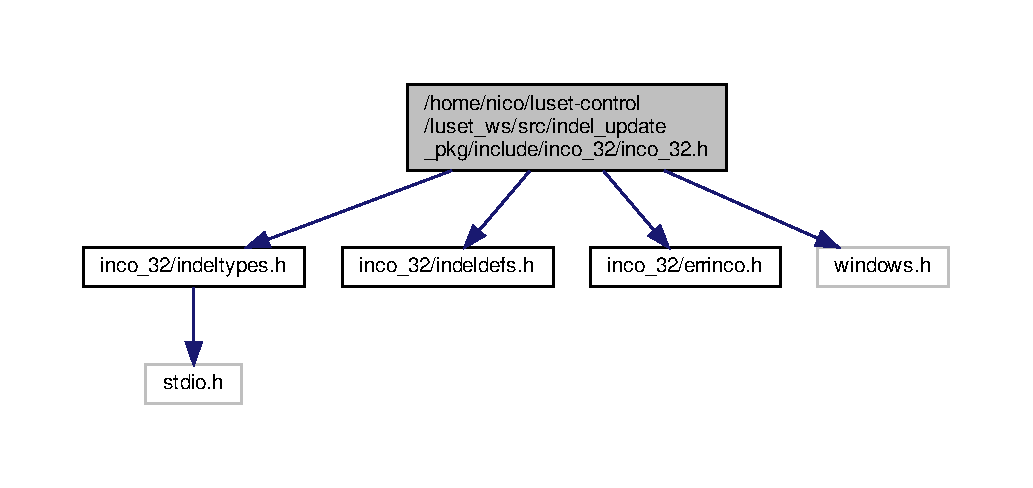
\includegraphics[width=350pt]{inco__32_8h__incl}
\end{center}
\end{figure}
This graph shows which files directly or indirectly include this file\+:\nopagebreak
\begin{figure}[H]
\begin{center}
\leavevmode
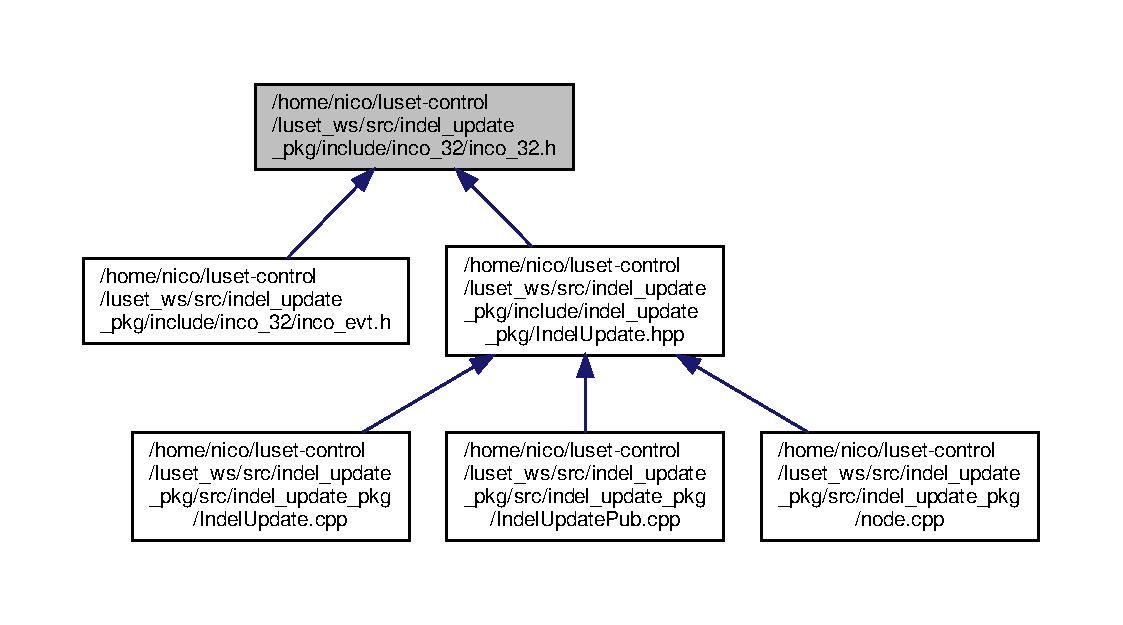
\includegraphics[width=350pt]{inco__32_8h__dep__incl}
\end{center}
\end{figure}
\subsection*{Macros}
\begin{DoxyCompactItemize}
\item 
\#define \hyperlink{inco__32_8h_a09505cad5bbb66fc36750a4fbca0444b}{I\+N\+C\+O32\+\_\+\+E\+X\+P\+O\+RT}~\+\_\+\+\_\+declspec(dllimport)
\item 
\#define \hyperlink{inco__32_8h_a751b0d6e0dbe97b2dfe601e4351840fd}{D\+F\+\_\+\+K\+E\+Y\+\_\+\+I\+N\+D\+E\+L\+\_\+\+P\+A\+T\+H\+\_\+\+D\+EP}~\char`\"{}S\+O\+F\+T\+W\+A\+R\+E\textbackslash{}\textbackslash{}\+Indel\char`\"{}
\item 
\#define \hyperlink{inco__32_8h_a7f4622a02facee9dd19b833b296bbabf}{D\+F\+\_\+\+T\+A\+S\+K\+\_\+\+N\+U\+M\+B\+E\+R\+\_\+\+O\+F\+\_\+\+G\+PR}~32
\item 
\#define \hyperlink{inco__32_8h_adf810ad67814631165612f65d7785d0a}{D\+F\+\_\+\+T\+A\+S\+K\+\_\+\+N\+U\+M\+B\+E\+R\+\_\+\+O\+F\+\_\+\+F\+PR}~32
\item 
\#define \hyperlink{inco__32_8h_a92190b5b7ec9e231a07798750e3de0b1}{D\+F\+\_\+\+T\+A\+S\+K\+\_\+\+N\+U\+M\+B\+E\+R\+\_\+\+O\+F\+\_\+\+S\+PR}~8
\end{DoxyCompactItemize}
\subsection*{Functions}
\begin{Indent}\textbf{ I\+N\+CO variable reading and writing}\par
\begin{DoxyCompactItemize}
\item 
\hyperlink{inco__32_8h_a09505cad5bbb66fc36750a4fbca0444b}{I\+N\+C\+O32\+\_\+\+E\+X\+P\+O\+RT} \hyperlink{indeltypes_8h_a4b435a49c74bb91f284f075e63416cb6}{uint32} W\+I\+N\+A\+PI \hyperlink{group__commonfunctions_ga5a35fc7cdfb6037cb755ed8409a8f300}{Get\+Variable} (const char $\ast$Target\+Path, const char $\ast$Item\+Path, void $\ast$Result, \hyperlink{indeltypes_8h_a4b435a49c74bb91f284f075e63416cb6}{uint32} Length)
\begin{DoxyCompactList}\small\item\em Remote I\+N\+CO variable read. \end{DoxyCompactList}\item 
\hyperlink{inco__32_8h_a09505cad5bbb66fc36750a4fbca0444b}{I\+N\+C\+O32\+\_\+\+E\+X\+P\+O\+RT} \hyperlink{indeltypes_8h_a4b435a49c74bb91f284f075e63416cb6}{uint32} W\+I\+N\+A\+PI \hyperlink{group__commonfunctions_gac50fba25dcc47ea6f6f54c0141e34563}{Put\+Variable} (const char $\ast$Target\+Path, const char $\ast$Item\+Path, const void $\ast$Value, \hyperlink{indeltypes_8h_a4b435a49c74bb91f284f075e63416cb6}{uint32} Length)
\begin{DoxyCompactList}\small\item\em Remote I\+N\+CO variable write. \end{DoxyCompactList}\end{DoxyCompactItemize}
\end{Indent}
\begin{Indent}\textbf{ Remote I\+N\+CO procedure call (R\+PC)}\par
{\em (see also syncasync) }\begin{DoxyCompactItemize}
\item 
\hyperlink{inco__32_8h_a09505cad5bbb66fc36750a4fbca0444b}{I\+N\+C\+O32\+\_\+\+E\+X\+P\+O\+RT} \hyperlink{indeltypes_8h_a4b435a49c74bb91f284f075e63416cb6}{uint32} W\+I\+N\+A\+PI \hyperlink{group__commonfunctions_gaa2b02d8d33d22482538bd936792904b1}{Call\+Procedure} (const char $\ast$Target\+Path, const char $\ast$Call\+Procedure, double $\ast$Result)
\begin{DoxyCompactList}\small\item\em Remote procedure call. \end{DoxyCompactList}\item 
\hyperlink{inco__32_8h_a09505cad5bbb66fc36750a4fbca0444b}{I\+N\+C\+O32\+\_\+\+E\+X\+P\+O\+RT} \hyperlink{indeltypes_8h_ac44d0188f4f50fd9b03031c1a06bd0a9}{int32} W\+I\+N\+A\+PI \hyperlink{group__commonfunctions_ga6b9c6b3f22614e8a2072f8c490402131}{Call\+Procedure\+Ex} (const char $\ast$Target\+Path, const char $\ast$\hyperlink{group__commonfunctions_gaa2b02d8d33d22482538bd936792904b1}{Call\+Procedure}, double $\ast$Sync\+Result)
\begin{DoxyCompactList}\small\item\em Remote procedure call (extended). \end{DoxyCompactList}\item 
\hyperlink{inco__32_8h_a09505cad5bbb66fc36750a4fbca0444b}{I\+N\+C\+O32\+\_\+\+E\+X\+P\+O\+RT} \hyperlink{indeltypes_8h_a4b435a49c74bb91f284f075e63416cb6}{uint32} W\+I\+N\+A\+PI \hyperlink{group__commonfunctions_ga7ea052077eebe514aa0cb1756c595189}{Call\+Procedure\+Ex\+Sync} (const char $\ast$Target\+Path, const char $\ast$\hyperlink{group__commonfunctions_gaa2b02d8d33d22482538bd936792904b1}{Call\+Procedure}, void $\ast$Result, \hyperlink{indeltypes_8h_a4b435a49c74bb91f284f075e63416cb6}{uint32} Buffer\+Size, \hyperlink{indeltypes_8h_a4b435a49c74bb91f284f075e63416cb6}{uint32} Type\+Flags)
\begin{DoxyCompactList}\small\item\em Remote procedure call (extended). If the procedure has an asynchronous part, the function will wait for it to complete. \end{DoxyCompactList}\item 
\hyperlink{inco__32_8h_a09505cad5bbb66fc36750a4fbca0444b}{I\+N\+C\+O32\+\_\+\+E\+X\+P\+O\+RT} \hyperlink{indeltypes_8h_a4b435a49c74bb91f284f075e63416cb6}{uint32} W\+I\+N\+A\+PI \hyperlink{group__commonfunctions_ga1b55ca711acd0dcc672e5fefe5cff27e}{Call\+Procedure\+Ex\+Wait} (const char $\ast$Target\+Path, \hyperlink{indeltypes_8h_ac44d0188f4f50fd9b03031c1a06bd0a9}{int32} Ticket, \hyperlink{indeltypes_8h_ac44d0188f4f50fd9b03031c1a06bd0a9}{int32} Timeout\+Ms)
\begin{DoxyCompactList}\small\item\em Wait for the asynchronous part of a remote procedure call (Call\+Procedure\+Ex) to finish (optionally with timeout). \end{DoxyCompactList}\item 
\hyperlink{inco__32_8h_a09505cad5bbb66fc36750a4fbca0444b}{I\+N\+C\+O32\+\_\+\+E\+X\+P\+O\+RT} \hyperlink{indeltypes_8h_a4b435a49c74bb91f284f075e63416cb6}{uint32} W\+I\+N\+A\+PI \hyperlink{group__commonfunctions_ga293b3f14ba486519c29ac9abfd0471e3}{Call\+Procedure\+Ex\+Result} (const char $\ast$Target\+Path, \hyperlink{indeltypes_8h_ac44d0188f4f50fd9b03031c1a06bd0a9}{int32} Ticket, void $\ast$Result, \hyperlink{indeltypes_8h_a4b435a49c74bb91f284f075e63416cb6}{uint32} Buffer\+Size, \hyperlink{indeltypes_8h_a4b435a49c74bb91f284f075e63416cb6}{uint32} Type\+Flags, char $\ast$Result\+Name, \hyperlink{indeltypes_8h_a4b435a49c74bb91f284f075e63416cb6}{uint32} Result\+Name\+Buf\+Size)
\begin{DoxyCompactList}\small\item\em Get the next asynchronous result (or application error) of a remote procedure call (Call\+Procedure\+Ex). \end{DoxyCompactList}\item 
\hyperlink{inco__32_8h_a09505cad5bbb66fc36750a4fbca0444b}{I\+N\+C\+O32\+\_\+\+E\+X\+P\+O\+RT} \hyperlink{indeltypes_8h_a4b435a49c74bb91f284f075e63416cb6}{uint32} W\+I\+N\+A\+PI \hyperlink{group__commonfunctions_ga569a93aeed06c2745365c881be5e7828}{Call\+Procedure\+Ex\+Result\+By\+Name} (const char $\ast$Target\+Path, \hyperlink{indeltypes_8h_ac44d0188f4f50fd9b03031c1a06bd0a9}{int32} Ticket, const char $\ast$Result\+Name, void $\ast$Result, \hyperlink{indeltypes_8h_a4b435a49c74bb91f284f075e63416cb6}{uint32} Buffer\+Size, \hyperlink{indeltypes_8h_a4b435a49c74bb91f284f075e63416cb6}{uint32} Type\+Flags)
\begin{DoxyCompactList}\small\item\em Get the next asynchronous named result (or application error) of a remote procedure call (Call\+Procedure\+Ex). \end{DoxyCompactList}\end{DoxyCompactItemize}
\end{Indent}
\begin{Indent}\textbf{ Raw target memory access functions}\par
\begin{DoxyCompactItemize}
\item 
\hyperlink{inco__32_8h_a09505cad5bbb66fc36750a4fbca0444b}{I\+N\+C\+O32\+\_\+\+E\+X\+P\+O\+RT} \hyperlink{indeltypes_8h_a4b435a49c74bb91f284f075e63416cb6}{uint32} W\+I\+N\+A\+PI \hyperlink{group__commonfunctions_ga7b0fc73de1e81c47c9ee82db36ea7d35}{Put\+Block8} (const char $\ast$Target\+Path, \hyperlink{indeltypes_8h_a4b435a49c74bb91f284f075e63416cb6}{uint32} Dest\+Address, const \hyperlink{indeltypes_8h_adde6aaee8457bee49c2a92621fe22b79}{uint8} $\ast$Data, \hyperlink{indeltypes_8h_a4b435a49c74bb91f284f075e63416cb6}{uint32} Number)
\begin{DoxyCompactList}\small\item\em Write raw data in 8 byte chunks to the target. \end{DoxyCompactList}\item 
\hyperlink{inco__32_8h_a09505cad5bbb66fc36750a4fbca0444b}{I\+N\+C\+O32\+\_\+\+E\+X\+P\+O\+RT} \hyperlink{indeltypes_8h_a4b435a49c74bb91f284f075e63416cb6}{uint32} W\+I\+N\+A\+PI \hyperlink{group__commonfunctions_gab25d23eaf697606036d12356f94fc675}{Get\+Block8} (const char $\ast$Target\+Path, \hyperlink{indeltypes_8h_a4b435a49c74bb91f284f075e63416cb6}{uint32} Source\+Address, \hyperlink{indeltypes_8h_adde6aaee8457bee49c2a92621fe22b79}{uint8} $\ast$Data, \hyperlink{indeltypes_8h_a4b435a49c74bb91f284f075e63416cb6}{uint32} Number)
\begin{DoxyCompactList}\small\item\em Reads raw data in 8 byte chunks from the target. \end{DoxyCompactList}\item 
\hyperlink{inco__32_8h_a09505cad5bbb66fc36750a4fbca0444b}{I\+N\+C\+O32\+\_\+\+E\+X\+P\+O\+RT} \hyperlink{indeltypes_8h_a4b435a49c74bb91f284f075e63416cb6}{uint32} W\+I\+N\+A\+PI \hyperlink{group__commonfunctions_gae156a8a2456bc41746e3452c609ee2fd}{Get\+Block8\+Real} (const char $\ast$Target\+Path, \hyperlink{indeltypes_8h_a4b435a49c74bb91f284f075e63416cb6}{uint32} Source\+Address, \hyperlink{indeltypes_8h_adde6aaee8457bee49c2a92621fe22b79}{uint8} $\ast$Data, \hyperlink{indeltypes_8h_a4b435a49c74bb91f284f075e63416cb6}{uint32} Number)
\begin{DoxyCompactList}\small\item\em For Indel internal use\+: Read 8 byte chunks of data from target by resolving breakpoints. \end{DoxyCompactList}\item 
\hyperlink{inco__32_8h_a09505cad5bbb66fc36750a4fbca0444b}{I\+N\+C\+O32\+\_\+\+E\+X\+P\+O\+RT} \hyperlink{indeltypes_8h_a4b435a49c74bb91f284f075e63416cb6}{uint32} W\+I\+N\+A\+PI \hyperlink{group__commonfunctions_ga385128fec8e3c887078779f2d8deb0fb}{Put\+Block16} (const char $\ast$Target\+Path, \hyperlink{indeltypes_8h_a4b435a49c74bb91f284f075e63416cb6}{uint32} Dest\+Address, const \hyperlink{indeltypes_8h_a05f6b0ae8f6a6e135b0e290c25fe0e4e}{uint16} $\ast$Data, \hyperlink{indeltypes_8h_a4b435a49c74bb91f284f075e63416cb6}{uint32} Number)
\begin{DoxyCompactList}\small\item\em Write raw data in 16 bytes chungs to the target. \end{DoxyCompactList}\item 
\hyperlink{inco__32_8h_a09505cad5bbb66fc36750a4fbca0444b}{I\+N\+C\+O32\+\_\+\+E\+X\+P\+O\+RT} \hyperlink{indeltypes_8h_a4b435a49c74bb91f284f075e63416cb6}{uint32} W\+I\+N\+A\+PI \hyperlink{group__commonfunctions_gae507b3a868c5004a2142190a48958d79}{Get\+Block16} (const char $\ast$Target\+Path, \hyperlink{indeltypes_8h_a4b435a49c74bb91f284f075e63416cb6}{uint32} Source\+Address, \hyperlink{indeltypes_8h_a05f6b0ae8f6a6e135b0e290c25fe0e4e}{uint16} $\ast$Data, \hyperlink{indeltypes_8h_a4b435a49c74bb91f284f075e63416cb6}{uint32} Number)
\begin{DoxyCompactList}\small\item\em Read raw data in 16 bytes chungs from the target. \end{DoxyCompactList}\item 
\hyperlink{inco__32_8h_a09505cad5bbb66fc36750a4fbca0444b}{I\+N\+C\+O32\+\_\+\+E\+X\+P\+O\+RT} \hyperlink{indeltypes_8h_a4b435a49c74bb91f284f075e63416cb6}{uint32} W\+I\+N\+A\+PI \hyperlink{group__commonfunctions_ga51c1743c005a868b73e6af8e96eb9d4e}{Put\+Block32} (const char $\ast$Target\+Path, \hyperlink{indeltypes_8h_a4b435a49c74bb91f284f075e63416cb6}{uint32} Dest\+Address, const \hyperlink{indeltypes_8h_a4b435a49c74bb91f284f075e63416cb6}{uint32} $\ast$Data, \hyperlink{indeltypes_8h_a4b435a49c74bb91f284f075e63416cb6}{uint32} Number)
\begin{DoxyCompactList}\small\item\em Write raw data in 32 bytes chungs to the target. \end{DoxyCompactList}\item 
\hyperlink{inco__32_8h_a09505cad5bbb66fc36750a4fbca0444b}{I\+N\+C\+O32\+\_\+\+E\+X\+P\+O\+RT} \hyperlink{indeltypes_8h_a4b435a49c74bb91f284f075e63416cb6}{uint32} W\+I\+N\+A\+PI \hyperlink{group__commonfunctions_ga25d9fc255f93000f56d0414339ac53e6}{Get\+Block32} (const char $\ast$Target\+Path, \hyperlink{indeltypes_8h_a4b435a49c74bb91f284f075e63416cb6}{uint32} Source\+Address, \hyperlink{indeltypes_8h_a4b435a49c74bb91f284f075e63416cb6}{uint32} $\ast$Data, \hyperlink{indeltypes_8h_a4b435a49c74bb91f284f075e63416cb6}{uint32} Number)
\begin{DoxyCompactList}\small\item\em Read raw data in 32 bytes chungs from the target. \end{DoxyCompactList}\item 
\hyperlink{inco__32_8h_a09505cad5bbb66fc36750a4fbca0444b}{I\+N\+C\+O32\+\_\+\+E\+X\+P\+O\+RT} \hyperlink{indeltypes_8h_a4b435a49c74bb91f284f075e63416cb6}{uint32} W\+I\+N\+A\+PI \hyperlink{group__commonfunctions_gaa67eff1b4ca61c6c9f1587bafa6e0a54}{Put\+Block64} (const char $\ast$Target\+Path, \hyperlink{indeltypes_8h_a4b435a49c74bb91f284f075e63416cb6}{uint32} Dest\+Address, const \hyperlink{indeltypes_8h_ac6afe794ed283c11fb63426a58188e5e}{uint64} $\ast$Data, \hyperlink{indeltypes_8h_a4b435a49c74bb91f284f075e63416cb6}{uint32} Number)
\begin{DoxyCompactList}\small\item\em Write raw data in 64 bytes chungs to the target. \end{DoxyCompactList}\item 
\hyperlink{inco__32_8h_a09505cad5bbb66fc36750a4fbca0444b}{I\+N\+C\+O32\+\_\+\+E\+X\+P\+O\+RT} \hyperlink{indeltypes_8h_a4b435a49c74bb91f284f075e63416cb6}{uint32} W\+I\+N\+A\+PI \hyperlink{group__commonfunctions_ga0dd1bf74ec3dd28ae6d784db54339802}{Get\+Block64} (const char $\ast$Target\+Path, \hyperlink{indeltypes_8h_a4b435a49c74bb91f284f075e63416cb6}{uint32} Source\+Address, \hyperlink{indeltypes_8h_ac6afe794ed283c11fb63426a58188e5e}{uint64} $\ast$Data, \hyperlink{indeltypes_8h_a4b435a49c74bb91f284f075e63416cb6}{uint32} Number)
\begin{DoxyCompactList}\small\item\em Read raw data in 64 bytes chungs from the target. \end{DoxyCompactList}\end{DoxyCompactItemize}
\end{Indent}
\begin{Indent}\textbf{ I\+N\+CO error information}\par
\begin{DoxyCompactItemize}
\item 
\hyperlink{inco__32_8h_a09505cad5bbb66fc36750a4fbca0444b}{I\+N\+C\+O32\+\_\+\+E\+X\+P\+O\+RT} \hyperlink{indeltypes_8h_a4b435a49c74bb91f284f075e63416cb6}{uint32} W\+I\+N\+A\+PI \hyperlink{group__commonfunctions_ga2ce71629197df864b4ca9121feaff795}{Get\+Error\+Description} (const char $\ast$Target\+Path, \hyperlink{indeltypes_8h_a4b435a49c74bb91f284f075e63416cb6}{uint32} Error, char $\ast$Description, \hyperlink{indeltypes_8h_a4b435a49c74bb91f284f075e63416cb6}{uint32} Length)
\begin{DoxyCompactList}\small\item\em Convert an I\+N\+CO error (see also incoreturn\+\_\+inco\+\_\+errors) to human readable string. \end{DoxyCompactList}\item 
\hyperlink{inco__32_8h_a09505cad5bbb66fc36750a4fbca0444b}{I\+N\+C\+O32\+\_\+\+E\+X\+P\+O\+RT} \hyperlink{indeltypes_8h_a4b435a49c74bb91f284f075e63416cb6}{uint32} W\+I\+N\+A\+PI \hyperlink{group__commonfunctions_gae35d1b67b8052ac2411a9c899141854f}{Get\+Mc\+Message} (const char $\ast$Target\+Path, const char $\ast$Message\+Handler\+Path, \hyperlink{indeltypes_8h_a4b435a49c74bb91f284f075e63416cb6}{uint32} Error, char $\ast$Message, \hyperlink{indeltypes_8h_a4b435a49c74bb91f284f075e63416cb6}{uint32} Length)
\end{DoxyCompactItemize}
\end{Indent}
\begin{Indent}\textbf{ I\+N\+C\+O32 version information}\par
\begin{DoxyCompactItemize}
\item 
\hyperlink{inco__32_8h_a09505cad5bbb66fc36750a4fbca0444b}{I\+N\+C\+O32\+\_\+\+E\+X\+P\+O\+RT} \hyperlink{indeltypes_8h_a4b435a49c74bb91f284f075e63416cb6}{uint32} W\+I\+N\+A\+PI \hyperlink{group__commonfunctions_gaae80abf7f7bc82fa98428b67da68a366}{Get\+Revisions} (const char $\ast$Target\+Path, \hyperlink{indeltypes_8h_a4b435a49c74bb91f284f075e63416cb6}{uint32} $\ast$Server\+Revision, \hyperlink{indeltypes_8h_a4b435a49c74bb91f284f075e63416cb6}{uint32} $\ast$Dll\+Revision)
\begin{DoxyCompactList}\small\item\em Function to get the I\+N\+C\+O\+Server and libinco\+\_\+32 revisions. \end{DoxyCompactList}\end{DoxyCompactItemize}
\end{Indent}
\begin{Indent}\textbf{ Database functions (for Indel internal use)}\par
\begin{DoxyCompactItemize}
\item 
\hyperlink{inco__32_8h_a09505cad5bbb66fc36750a4fbca0444b}{I\+N\+C\+O32\+\_\+\+E\+X\+P\+O\+RT} \hyperlink{indeltypes_8h_a4b435a49c74bb91f284f075e63416cb6}{uint32} W\+I\+N\+A\+PI \hyperlink{inco__32_8h_a1cb03b74d464f1550394843cf7199283}{Create\+Table} (const char $\ast$Target\+Path, const char $\ast$Table\+Name, const char $\ast$Database\+Name, \hyperlink{indeltypes_8h_a4b435a49c74bb91f284f075e63416cb6}{uint32} Number\+Records, \hyperlink{indeltypes_8h_a4b435a49c74bb91f284f075e63416cb6}{uint32} Record\+Size, \hyperlink{indeltypes_8h_a4b435a49c74bb91f284f075e63416cb6}{uint32} Flags)
\item 
\hyperlink{inco__32_8h_a09505cad5bbb66fc36750a4fbca0444b}{I\+N\+C\+O32\+\_\+\+E\+X\+P\+O\+RT} \hyperlink{indeltypes_8h_a4b435a49c74bb91f284f075e63416cb6}{uint32} W\+I\+N\+A\+PI \hyperlink{inco__32_8h_a40d41d06d78b22fe59b86148b6892d33}{Delete\+Table} (const char $\ast$Target\+Path, const char $\ast$Table\+Name)
\item 
\hyperlink{inco__32_8h_a09505cad5bbb66fc36750a4fbca0444b}{I\+N\+C\+O32\+\_\+\+E\+X\+P\+O\+RT} \hyperlink{indeltypes_8h_a4b435a49c74bb91f284f075e63416cb6}{uint32} W\+I\+N\+A\+PI \hyperlink{inco__32_8h_a203a38d0771e315d0f89aad8451eab9a}{Put\+Record} (const char $\ast$Target\+Path, const char $\ast$Table\+Name, const char $\ast$Record, void $\ast$Data, \hyperlink{indeltypes_8h_a4b435a49c74bb91f284f075e63416cb6}{uint32} Size)
\item 
\hyperlink{inco__32_8h_a09505cad5bbb66fc36750a4fbca0444b}{I\+N\+C\+O32\+\_\+\+E\+X\+P\+O\+RT} \hyperlink{indeltypes_8h_a4b435a49c74bb91f284f075e63416cb6}{uint32} W\+I\+N\+A\+PI \hyperlink{inco__32_8h_aa0e9d2065b1b6402b6e25f0362264bb8}{Get\+Record} (const char $\ast$Target\+Path, const char $\ast$Table\+Name, const char $\ast$Record, void $\ast$Data, \hyperlink{indeltypes_8h_a4b435a49c74bb91f284f075e63416cb6}{uint32} Size)
\end{DoxyCompactItemize}
\end{Indent}
\begin{Indent}\textbf{ Target\+Path debugging functionality (for Indel internal use)}\par
\begin{DoxyCompactItemize}
\item 
\hyperlink{inco__32_8h_a09505cad5bbb66fc36750a4fbca0444b}{I\+N\+C\+O32\+\_\+\+E\+X\+P\+O\+RT} \hyperlink{indeltypes_8h_a4b435a49c74bb91f284f075e63416cb6}{uint32} W\+I\+N\+A\+PI \hyperlink{inco__32_8h_af34af3141e14ab0549b1ba44e1f0892d}{Dbg\+Os\+Prepare\+Load} (const char $\ast$Target\+Path)
\item 
\hyperlink{inco__32_8h_a09505cad5bbb66fc36750a4fbca0444b}{I\+N\+C\+O32\+\_\+\+E\+X\+P\+O\+RT} \hyperlink{indeltypes_8h_a4b435a49c74bb91f284f075e63416cb6}{uint32} W\+I\+N\+A\+PI \hyperlink{inco__32_8h_ad1f06dea244943176d0d98dbc003ead8}{Dbg\+Os\+Reset} (const char $\ast$Target\+Path, \hyperlink{indeltypes_8h_a4b435a49c74bb91f284f075e63416cb6}{uint32} a\+Flags)
\item 
\hyperlink{inco__32_8h_a09505cad5bbb66fc36750a4fbca0444b}{I\+N\+C\+O32\+\_\+\+E\+X\+P\+O\+RT} \hyperlink{indeltypes_8h_a4b435a49c74bb91f284f075e63416cb6}{uint32} W\+I\+N\+A\+PI \hyperlink{inco__32_8h_ae78dfd6c87f4227b40a9a42df9984011}{Dbg\+Tasks\+List} (const char $\ast$Target\+Path, void $\ast$a\+Result, \hyperlink{indeltypes_8h_a4b435a49c74bb91f284f075e63416cb6}{uint32} a\+Length)
\item 
\hyperlink{inco__32_8h_a09505cad5bbb66fc36750a4fbca0444b}{I\+N\+C\+O32\+\_\+\+E\+X\+P\+O\+RT} \hyperlink{indeltypes_8h_a4b435a49c74bb91f284f075e63416cb6}{uint32} W\+I\+N\+A\+PI \hyperlink{inco__32_8h_afce3373c2e1911343767b453ca6d1d0c}{Dbg\+Tasks\+State} (const char $\ast$Target\+Path, void $\ast$a\+Result, \hyperlink{indeltypes_8h_a4b435a49c74bb91f284f075e63416cb6}{uint32} a\+Length)
\item 
\hyperlink{inco__32_8h_a09505cad5bbb66fc36750a4fbca0444b}{I\+N\+C\+O32\+\_\+\+E\+X\+P\+O\+RT} \hyperlink{indeltypes_8h_a4b435a49c74bb91f284f075e63416cb6}{uint32} W\+I\+N\+A\+PI \hyperlink{inco__32_8h_a2a7045977dbb92ddcd3fce232515e894}{Dbg\+Task\+Get\+Id} (const char $\ast$Target\+Path, const char $\ast$a\+Task\+Name, \hyperlink{indeltypes_8h_a4b435a49c74bb91f284f075e63416cb6}{uint32} $\ast$a\+Task\+Id)
\item 
\hyperlink{inco__32_8h_a09505cad5bbb66fc36750a4fbca0444b}{I\+N\+C\+O32\+\_\+\+E\+X\+P\+O\+RT} \hyperlink{indeltypes_8h_a4b435a49c74bb91f284f075e63416cb6}{uint32} W\+I\+N\+A\+PI \hyperlink{inco__32_8h_ad4628b0c16f0bbaad767fdb910ea4449}{Dbg\+Task\+Set\+Breakpoint} (const char $\ast$Target\+Path, const char $\ast$a\+Task\+Name, \hyperlink{indeltypes_8h_a4b435a49c74bb91f284f075e63416cb6}{uint32} a\+Address)
\item 
\hyperlink{inco__32_8h_a09505cad5bbb66fc36750a4fbca0444b}{I\+N\+C\+O32\+\_\+\+E\+X\+P\+O\+RT} \hyperlink{indeltypes_8h_a4b435a49c74bb91f284f075e63416cb6}{uint32} W\+I\+N\+A\+PI \hyperlink{inco__32_8h_ad01a7dd197ffcdffc68f8abd11b5c600}{Dbg\+Task\+Clr\+Breakpoint} (const char $\ast$Target\+Path, const char $\ast$a\+Task\+Name, \hyperlink{indeltypes_8h_a4b435a49c74bb91f284f075e63416cb6}{uint32} a\+Address)
\item 
\hyperlink{inco__32_8h_a09505cad5bbb66fc36750a4fbca0444b}{I\+N\+C\+O32\+\_\+\+E\+X\+P\+O\+RT} \hyperlink{indeltypes_8h_a4b435a49c74bb91f284f075e63416cb6}{uint32} W\+I\+N\+A\+PI \hyperlink{inco__32_8h_a9732c1cdd1052d9e08466fe1cfe40f21}{Dbg\+Task\+Get\+Breakpoint} (const char $\ast$Target\+Path, \hyperlink{indeltypes_8h_a4b435a49c74bb91f284f075e63416cb6}{uint32} a\+Number, void $\ast$a\+Result, \hyperlink{indeltypes_8h_a4b435a49c74bb91f284f075e63416cb6}{uint32} a\+Length)
\item 
\hyperlink{inco__32_8h_a09505cad5bbb66fc36750a4fbca0444b}{I\+N\+C\+O32\+\_\+\+E\+X\+P\+O\+RT} \hyperlink{indeltypes_8h_a4b435a49c74bb91f284f075e63416cb6}{uint32} W\+I\+N\+A\+PI \hyperlink{inco__32_8h_a7e3c86c108b3b5c8c940a84d109c93c4}{Dbg\+Task\+Get\+Name} (const char $\ast$Target\+Path, \hyperlink{indeltypes_8h_a4b435a49c74bb91f284f075e63416cb6}{uint32} a\+Task\+Id, char $\ast$a\+Task\+Name, \hyperlink{indeltypes_8h_a4b435a49c74bb91f284f075e63416cb6}{uint32} a\+Length)
\item 
\hyperlink{inco__32_8h_a09505cad5bbb66fc36750a4fbca0444b}{I\+N\+C\+O32\+\_\+\+E\+X\+P\+O\+RT} \hyperlink{indeltypes_8h_a4b435a49c74bb91f284f075e63416cb6}{uint32} W\+I\+N\+A\+PI \hyperlink{inco__32_8h_ae623f14cd8536909d776f831e37e0c06}{Dbg\+Task\+Halt} (const char $\ast$Target\+Path, \hyperlink{indeltypes_8h_a4b435a49c74bb91f284f075e63416cb6}{uint32} a\+Task\+Id)
\item 
\hyperlink{inco__32_8h_a09505cad5bbb66fc36750a4fbca0444b}{I\+N\+C\+O32\+\_\+\+E\+X\+P\+O\+RT} \hyperlink{indeltypes_8h_a4b435a49c74bb91f284f075e63416cb6}{uint32} W\+I\+N\+A\+PI \hyperlink{inco__32_8h_a1ff670a770219174c76034b37e03b0ed}{Dbg\+Task\+Run} (const char $\ast$Target\+Path, \hyperlink{indeltypes_8h_a4b435a49c74bb91f284f075e63416cb6}{uint32} a\+Task\+Id)
\item 
\hyperlink{inco__32_8h_a09505cad5bbb66fc36750a4fbca0444b}{I\+N\+C\+O32\+\_\+\+E\+X\+P\+O\+RT} \hyperlink{indeltypes_8h_a4b435a49c74bb91f284f075e63416cb6}{uint32} W\+I\+N\+A\+PI \hyperlink{inco__32_8h_aada24dbbf9c30e3d79cca5d29dc1e6f3}{Dbg\+Task\+Single\+Step} (const char $\ast$Target\+Path, \hyperlink{indeltypes_8h_a4b435a49c74bb91f284f075e63416cb6}{uint32} a\+Task\+Id)
\item 
\hyperlink{inco__32_8h_a09505cad5bbb66fc36750a4fbca0444b}{I\+N\+C\+O32\+\_\+\+E\+X\+P\+O\+RT} \hyperlink{indeltypes_8h_a4b435a49c74bb91f284f075e63416cb6}{uint32} W\+I\+N\+A\+PI \hyperlink{inco__32_8h_adf14fb123b066d4e52d0c41bf150a0aa}{Dbg\+Task\+Range\+Step} (const char $\ast$Target\+Path, \hyperlink{indeltypes_8h_a4b435a49c74bb91f284f075e63416cb6}{uint32} a\+Task\+Id, \hyperlink{indeltypes_8h_a4b435a49c74bb91f284f075e63416cb6}{uint32} au\+From, \hyperlink{indeltypes_8h_a4b435a49c74bb91f284f075e63416cb6}{uint32} au\+To)
\item 
\hyperlink{inco__32_8h_a09505cad5bbb66fc36750a4fbca0444b}{I\+N\+C\+O32\+\_\+\+E\+X\+P\+O\+RT} \hyperlink{indeltypes_8h_a4b435a49c74bb91f284f075e63416cb6}{uint32} W\+I\+N\+A\+PI \hyperlink{inco__32_8h_aad05378d496c4e013b157334f5d80c9e}{Dbg\+Task\+Get\+G\+P\+Rs} (const char $\ast$Target\+Path, \hyperlink{indeltypes_8h_a4b435a49c74bb91f284f075e63416cb6}{uint32} a\+Task\+Id, \hyperlink{indeltypes_8h_a4b435a49c74bb91f284f075e63416cb6}{uint32}($\ast$a\+Result)\mbox{[}\hyperlink{inco__32_8h_a7f4622a02facee9dd19b833b296bbabf}{D\+F\+\_\+\+T\+A\+S\+K\+\_\+\+N\+U\+M\+B\+E\+R\+\_\+\+O\+F\+\_\+\+G\+PR}\mbox{]})
\item 
\hyperlink{inco__32_8h_a09505cad5bbb66fc36750a4fbca0444b}{I\+N\+C\+O32\+\_\+\+E\+X\+P\+O\+RT} \hyperlink{indeltypes_8h_a4b435a49c74bb91f284f075e63416cb6}{uint32} W\+I\+N\+A\+PI \hyperlink{inco__32_8h_a4a7fcfe75e3c5f6cf94c46dfcf99ec64}{Dbg\+Task\+Get\+F\+P\+Rs} (const char $\ast$Target\+Path, \hyperlink{indeltypes_8h_a4b435a49c74bb91f284f075e63416cb6}{uint32} a\+Task\+Id, double($\ast$a\+Result)\mbox{[}\hyperlink{inco__32_8h_adf810ad67814631165612f65d7785d0a}{D\+F\+\_\+\+T\+A\+S\+K\+\_\+\+N\+U\+M\+B\+E\+R\+\_\+\+O\+F\+\_\+\+F\+PR}\mbox{]})
\item 
\hyperlink{inco__32_8h_a09505cad5bbb66fc36750a4fbca0444b}{I\+N\+C\+O32\+\_\+\+E\+X\+P\+O\+RT} \hyperlink{indeltypes_8h_a4b435a49c74bb91f284f075e63416cb6}{uint32} W\+I\+N\+A\+PI \hyperlink{inco__32_8h_a693cfbadfb9a692cbaff870720f721c2}{Dbg\+Task\+Get\+S\+P\+Rs} (const char $\ast$Target\+Path, \hyperlink{indeltypes_8h_a4b435a49c74bb91f284f075e63416cb6}{uint32} a\+Task\+Id, \hyperlink{indeltypes_8h_a4b435a49c74bb91f284f075e63416cb6}{uint32}($\ast$a\+Result)\mbox{[}\hyperlink{inco__32_8h_a92190b5b7ec9e231a07798750e3de0b1}{D\+F\+\_\+\+T\+A\+S\+K\+\_\+\+N\+U\+M\+B\+E\+R\+\_\+\+O\+F\+\_\+\+S\+PR}\mbox{]})
\item 
\hyperlink{inco__32_8h_a09505cad5bbb66fc36750a4fbca0444b}{I\+N\+C\+O32\+\_\+\+E\+X\+P\+O\+RT} \hyperlink{indeltypes_8h_a4b435a49c74bb91f284f075e63416cb6}{uint32} W\+I\+N\+A\+PI \hyperlink{inco__32_8h_a7f8e2516bd2936fc4e3392edb05cb33d}{Dbg\+Task\+Get\+G\+PR} (const char $\ast$Target\+Path, \hyperlink{indeltypes_8h_a4b435a49c74bb91f284f075e63416cb6}{uint32} a\+Task\+Id, \hyperlink{indeltypes_8h_a4b435a49c74bb91f284f075e63416cb6}{uint32} a\+Number, \hyperlink{indeltypes_8h_a4b435a49c74bb91f284f075e63416cb6}{uint32} $\ast$a\+Value)
\item 
\hyperlink{inco__32_8h_a09505cad5bbb66fc36750a4fbca0444b}{I\+N\+C\+O32\+\_\+\+E\+X\+P\+O\+RT} \hyperlink{indeltypes_8h_a4b435a49c74bb91f284f075e63416cb6}{uint32} W\+I\+N\+A\+PI \hyperlink{inco__32_8h_a9f97309065b9a45babfd5a631d3b6e6a}{Dbg\+Task\+Get\+F\+PR} (const char $\ast$Target\+Path, \hyperlink{indeltypes_8h_a4b435a49c74bb91f284f075e63416cb6}{uint32} a\+Task\+Id, \hyperlink{indeltypes_8h_a4b435a49c74bb91f284f075e63416cb6}{uint32} a\+Number, double $\ast$a\+Value)
\item 
\hyperlink{inco__32_8h_a09505cad5bbb66fc36750a4fbca0444b}{I\+N\+C\+O32\+\_\+\+E\+X\+P\+O\+RT} \hyperlink{indeltypes_8h_a4b435a49c74bb91f284f075e63416cb6}{uint32} W\+I\+N\+A\+PI \hyperlink{inco__32_8h_aabd0c9322c6f15e0ff4cf174f673794c}{Dbg\+Task\+Get\+S\+PR} (const char $\ast$Target\+Path, \hyperlink{indeltypes_8h_a4b435a49c74bb91f284f075e63416cb6}{uint32} a\+Task\+Id, \hyperlink{indeltypes_8h_a4b435a49c74bb91f284f075e63416cb6}{uint32} a\+Number, \hyperlink{indeltypes_8h_a4b435a49c74bb91f284f075e63416cb6}{uint32} $\ast$a\+Value)
\item 
\hyperlink{inco__32_8h_a09505cad5bbb66fc36750a4fbca0444b}{I\+N\+C\+O32\+\_\+\+E\+X\+P\+O\+RT} \hyperlink{indeltypes_8h_a4b435a49c74bb91f284f075e63416cb6}{uint32} W\+I\+N\+A\+PI \hyperlink{inco__32_8h_a30e9a2a6631a488450181e32dbf7063e}{Dbg\+Task\+Put\+G\+PR} (const char $\ast$Target\+Path, \hyperlink{indeltypes_8h_a4b435a49c74bb91f284f075e63416cb6}{uint32} a\+Task\+Id, \hyperlink{indeltypes_8h_a4b435a49c74bb91f284f075e63416cb6}{uint32} a\+Number, \hyperlink{indeltypes_8h_a4b435a49c74bb91f284f075e63416cb6}{uint32} a\+Value)
\item 
\hyperlink{inco__32_8h_a09505cad5bbb66fc36750a4fbca0444b}{I\+N\+C\+O32\+\_\+\+E\+X\+P\+O\+RT} \hyperlink{indeltypes_8h_a4b435a49c74bb91f284f075e63416cb6}{uint32} W\+I\+N\+A\+PI \hyperlink{inco__32_8h_ae5aa5559253be22f23ae5a090fbcb39f}{Dbg\+Task\+Put\+F\+PR} (const char $\ast$Target\+Path, \hyperlink{indeltypes_8h_a4b435a49c74bb91f284f075e63416cb6}{uint32} a\+Task\+Id, \hyperlink{indeltypes_8h_a4b435a49c74bb91f284f075e63416cb6}{uint32} a\+Number, double a\+Value)
\item 
\hyperlink{inco__32_8h_a09505cad5bbb66fc36750a4fbca0444b}{I\+N\+C\+O32\+\_\+\+E\+X\+P\+O\+RT} \hyperlink{indeltypes_8h_a4b435a49c74bb91f284f075e63416cb6}{uint32} W\+I\+N\+A\+PI \hyperlink{inco__32_8h_a503940920fffec3f2ca580e4ad50f3db}{Dbg\+Task\+Put\+S\+PR} (const char $\ast$Target\+Path, \hyperlink{indeltypes_8h_a4b435a49c74bb91f284f075e63416cb6}{uint32} a\+Task\+Id, \hyperlink{indeltypes_8h_a4b435a49c74bb91f284f075e63416cb6}{uint32} a\+Number, \hyperlink{indeltypes_8h_a4b435a49c74bb91f284f075e63416cb6}{uint32} a\+Value)
\item 
\hyperlink{inco__32_8h_a09505cad5bbb66fc36750a4fbca0444b}{I\+N\+C\+O32\+\_\+\+E\+X\+P\+O\+RT} \hyperlink{indeltypes_8h_a4b435a49c74bb91f284f075e63416cb6}{uint32} W\+I\+N\+A\+PI \hyperlink{inco__32_8h_aadf3cff89a7c86c152e7cd03cdf83e68}{Dbg\+Task\+Get\+Data} (const char $\ast$Target\+Path, \hyperlink{indeltypes_8h_a4b435a49c74bb91f284f075e63416cb6}{uint32} a\+Task\+Id, \hyperlink{indeltypes_8h_a4b435a49c74bb91f284f075e63416cb6}{uint32} a\+Data\+Def, void $\ast$a\+Result, \hyperlink{indeltypes_8h_a4b435a49c74bb91f284f075e63416cb6}{uint32} a\+Length)
\item 
\hyperlink{inco__32_8h_a09505cad5bbb66fc36750a4fbca0444b}{I\+N\+C\+O32\+\_\+\+E\+X\+P\+O\+RT} \hyperlink{indeltypes_8h_a4b435a49c74bb91f284f075e63416cb6}{uint32} W\+I\+N\+A\+PI \hyperlink{inco__32_8h_ad127120315a2797bb94bf04886ce0629}{Dbg\+Task\+Put\+Data} (const char $\ast$Target\+Path, \hyperlink{indeltypes_8h_a4b435a49c74bb91f284f075e63416cb6}{uint32} a\+Task\+Id, \hyperlink{indeltypes_8h_a4b435a49c74bb91f284f075e63416cb6}{uint32} a\+Data\+Def, void $\ast$a\+Data, \hyperlink{indeltypes_8h_a4b435a49c74bb91f284f075e63416cb6}{uint32} a\+Length)
\item 
\hyperlink{inco__32_8h_a09505cad5bbb66fc36750a4fbca0444b}{I\+N\+C\+O32\+\_\+\+E\+X\+P\+O\+RT} \hyperlink{indeltypes_8h_a4b435a49c74bb91f284f075e63416cb6}{uint32} W\+I\+N\+A\+PI \hyperlink{inco__32_8h_a75fc64e252c0532fd4136374c1e0ccc3}{Dbg\+Cpu\+Get\+S\+PR} (const char $\ast$Target\+Path, \hyperlink{indeltypes_8h_a4b435a49c74bb91f284f075e63416cb6}{uint32} a\+Number, \hyperlink{indeltypes_8h_a4b435a49c74bb91f284f075e63416cb6}{uint32} $\ast$a\+Result)
\item 
\hyperlink{inco__32_8h_a09505cad5bbb66fc36750a4fbca0444b}{I\+N\+C\+O32\+\_\+\+E\+X\+P\+O\+RT} \hyperlink{indeltypes_8h_a4b435a49c74bb91f284f075e63416cb6}{uint32} W\+I\+N\+A\+PI \hyperlink{inco__32_8h_a0d9d7cdc7df20344a8e50a0d83af570b}{Dbg\+Cpu\+Put\+S\+PR} (const char $\ast$Target\+Path, \hyperlink{indeltypes_8h_a4b435a49c74bb91f284f075e63416cb6}{uint32} a\+Number, \hyperlink{indeltypes_8h_a4b435a49c74bb91f284f075e63416cb6}{uint32} a\+Value)
\item 
\hyperlink{inco__32_8h_a09505cad5bbb66fc36750a4fbca0444b}{I\+N\+C\+O32\+\_\+\+E\+X\+P\+O\+RT} \hyperlink{indeltypes_8h_a4b435a49c74bb91f284f075e63416cb6}{uint32} W\+I\+N\+A\+PI \hyperlink{inco__32_8h_ad1bd14229e259161548a6029ebce8200}{Dbg\+Cpu\+Get\+D\+CR} (const char $\ast$Target\+Path, \hyperlink{indeltypes_8h_a4b435a49c74bb91f284f075e63416cb6}{uint32} a\+Number, \hyperlink{indeltypes_8h_a4b435a49c74bb91f284f075e63416cb6}{uint32} $\ast$a\+Result)
\item 
\hyperlink{inco__32_8h_a09505cad5bbb66fc36750a4fbca0444b}{I\+N\+C\+O32\+\_\+\+E\+X\+P\+O\+RT} \hyperlink{indeltypes_8h_a4b435a49c74bb91f284f075e63416cb6}{uint32} W\+I\+N\+A\+PI \hyperlink{inco__32_8h_a240fceb2151a880c78dcb5ab70a05df5}{Dbg\+Cpu\+Put\+D\+CR} (const char $\ast$Target\+Path, \hyperlink{indeltypes_8h_a4b435a49c74bb91f284f075e63416cb6}{uint32} a\+Number, \hyperlink{indeltypes_8h_a4b435a49c74bb91f284f075e63416cb6}{uint32} a\+Value)
\item 
\hyperlink{inco__32_8h_a09505cad5bbb66fc36750a4fbca0444b}{I\+N\+C\+O32\+\_\+\+E\+X\+P\+O\+RT} \hyperlink{indeltypes_8h_a4b435a49c74bb91f284f075e63416cb6}{uint32} W\+I\+N\+A\+PI \hyperlink{inco__32_8h_a8ad8a94e33e545389c3e813d7ad85e31}{Dbg\+Eme\+Comm\+Status} (const char $\ast$Target\+Path, \hyperlink{indeltypes_8h_a4b435a49c74bb91f284f075e63416cb6}{uint32} $\ast$ap\+Eme\+Comm\+Status)
\item 
\hyperlink{inco__32_8h_a09505cad5bbb66fc36750a4fbca0444b}{I\+N\+C\+O32\+\_\+\+E\+X\+P\+O\+RT} \hyperlink{indeltypes_8h_a4b435a49c74bb91f284f075e63416cb6}{uint32} W\+I\+N\+A\+PI \hyperlink{inco__32_8h_afbc6ae790e7a24a0e00f0c825a392167}{Dbg\+Os\+Continue} (const char $\ast$Target\+Path, \hyperlink{indeltypes_8h_a4b435a49c74bb91f284f075e63416cb6}{uint32} au\+Flags)
\item 
\hyperlink{inco__32_8h_a09505cad5bbb66fc36750a4fbca0444b}{I\+N\+C\+O32\+\_\+\+E\+X\+P\+O\+RT} \hyperlink{indeltypes_8h_a4b435a49c74bb91f284f075e63416cb6}{uint32} W\+I\+N\+A\+PI \hyperlink{inco__32_8h_a1626ac2589ae0fb1beccde520e8aab72}{Dbg\+Task\+Get\+Reg} (const char $\ast$Target\+Path, \hyperlink{indeltypes_8h_a4b435a49c74bb91f284f075e63416cb6}{uint32} a\+Task\+Id, \hyperlink{indeltypes_8h_a4b435a49c74bb91f284f075e63416cb6}{uint32} $\ast$ap\+Cookie, \hyperlink{indeltypes_8h_a4b435a49c74bb91f284f075e63416cb6}{uint32} $\ast$ap\+Flags, void $\ast$ap\+Buffer, \hyperlink{indeltypes_8h_a4b435a49c74bb91f284f075e63416cb6}{uint32} $\ast$ap\+Buffer\+Length)
\item 
\hyperlink{inco__32_8h_a09505cad5bbb66fc36750a4fbca0444b}{I\+N\+C\+O32\+\_\+\+E\+X\+P\+O\+RT} \hyperlink{indeltypes_8h_a4b435a49c74bb91f284f075e63416cb6}{uint32} W\+I\+N\+A\+PI \hyperlink{inco__32_8h_a62547879476d6c476a85ff5206b3656d}{Dbg\+Set\+Watchpoint} (const char $\ast$Target\+Path, \hyperlink{indeltypes_8h_a4b435a49c74bb91f284f075e63416cb6}{uint32} au\+Address, \hyperlink{indeltypes_8h_a4b435a49c74bb91f284f075e63416cb6}{uint32} au\+Size, \hyperlink{indeltypes_8h_a4b435a49c74bb91f284f075e63416cb6}{uint32} au\+Flags, \hyperlink{indeltypes_8h_a4b435a49c74bb91f284f075e63416cb6}{uint32} $\ast$ap\+Address, \hyperlink{indeltypes_8h_a4b435a49c74bb91f284f075e63416cb6}{uint32} $\ast$ap\+Size)
\item 
\hyperlink{inco__32_8h_a09505cad5bbb66fc36750a4fbca0444b}{I\+N\+C\+O32\+\_\+\+E\+X\+P\+O\+RT} \hyperlink{indeltypes_8h_a4b435a49c74bb91f284f075e63416cb6}{uint32} W\+I\+N\+A\+PI \hyperlink{inco__32_8h_acd921a56a65f69db5afbe9c789624fa3}{Dbg\+Clr\+Watchpoint} (const char $\ast$Target\+Path, \hyperlink{indeltypes_8h_a4b435a49c74bb91f284f075e63416cb6}{uint32} au\+Address)
\item 
\hyperlink{inco__32_8h_a09505cad5bbb66fc36750a4fbca0444b}{I\+N\+C\+O32\+\_\+\+E\+X\+P\+O\+RT} \hyperlink{indeltypes_8h_a4b435a49c74bb91f284f075e63416cb6}{uint32} W\+I\+N\+A\+PI \hyperlink{inco__32_8h_a9e562e9e518b0507bf4599e67090d99a}{Dbg\+Target\+Get\+Data\+Multi} (const char $\ast$Target\+Path, \hyperlink{indeltypes_8h_a4b435a49c74bb91f284f075e63416cb6}{uint32} $\ast$ap\+Cookie, \hyperlink{indeltypes_8h_a4b435a49c74bb91f284f075e63416cb6}{uint32} $\ast$ap\+Flags, void $\ast$ap\+Buffer, \hyperlink{indeltypes_8h_a4b435a49c74bb91f284f075e63416cb6}{uint32} $\ast$ap\+Buffer\+Length, \hyperlink{indeltypes_8h_a4b435a49c74bb91f284f075e63416cb6}{uint32} $\ast$ap\+Remaining\+Data\+Length)
\item 
\hyperlink{inco__32_8h_a09505cad5bbb66fc36750a4fbca0444b}{I\+N\+C\+O32\+\_\+\+E\+X\+P\+O\+RT} \hyperlink{indeltypes_8h_a4b435a49c74bb91f284f075e63416cb6}{uint32} W\+I\+N\+A\+PI \hyperlink{inco__32_8h_a470eab2b974686bebf234b87a57c17f4}{Dbg\+Task\+Get\+Data\+Multi} (const char $\ast$Target\+Path, \hyperlink{indeltypes_8h_a4b435a49c74bb91f284f075e63416cb6}{uint32} a\+Task\+Id, \hyperlink{indeltypes_8h_a4b435a49c74bb91f284f075e63416cb6}{uint32} $\ast$ap\+Cookie, \hyperlink{indeltypes_8h_a4b435a49c74bb91f284f075e63416cb6}{uint32} $\ast$ap\+Flags, void $\ast$ap\+Buffer, \hyperlink{indeltypes_8h_a4b435a49c74bb91f284f075e63416cb6}{uint32} $\ast$ap\+Buffer\+Length, \hyperlink{indeltypes_8h_a4b435a49c74bb91f284f075e63416cb6}{uint32} $\ast$ap\+Remaining\+Data\+Length)
\item 
\hyperlink{inco__32_8h_a09505cad5bbb66fc36750a4fbca0444b}{I\+N\+C\+O32\+\_\+\+E\+X\+P\+O\+RT} \hyperlink{indeltypes_8h_a4b435a49c74bb91f284f075e63416cb6}{uint32} W\+I\+N\+A\+PI \hyperlink{inco__32_8h_a80705c014b81ac6f072d095ce5e44487}{Dbg\+Task\+Get\+Data\+From\+Cache} (const char $\ast$Target\+Path, \hyperlink{indeltypes_8h_a4b435a49c74bb91f284f075e63416cb6}{uint32} $\ast$ap\+Cookie, \hyperlink{indeltypes_8h_a4b435a49c74bb91f284f075e63416cb6}{uint32} $\ast$ap\+Flags, void $\ast$ap\+Buffer, \hyperlink{indeltypes_8h_a4b435a49c74bb91f284f075e63416cb6}{uint32} $\ast$ap\+Buffer\+Length, \hyperlink{indeltypes_8h_a4b435a49c74bb91f284f075e63416cb6}{uint32} $\ast$ap\+Remaining\+Data\+Length)
\item 
\hyperlink{inco__32_8h_a09505cad5bbb66fc36750a4fbca0444b}{I\+N\+C\+O32\+\_\+\+E\+X\+P\+O\+RT} \hyperlink{indeltypes_8h_a4b435a49c74bb91f284f075e63416cb6}{uint32} W\+I\+N\+A\+PI \hyperlink{inco__32_8h_a0734aa727c2b39617ebc07790cbd809f}{Dbg\+Task\+Put\+Gdb\+Reg} (const char $\ast$Target\+Path, \hyperlink{indeltypes_8h_a4b435a49c74bb91f284f075e63416cb6}{uint32} a\+Task\+Id, const \hyperlink{indeltypes_8h_a4b435a49c74bb91f284f075e63416cb6}{uint32} au\+Register, const void $\ast$ap\+Data, \hyperlink{indeltypes_8h_a4b435a49c74bb91f284f075e63416cb6}{uint32} au\+Data\+Length)
\end{DoxyCompactItemize}
\end{Indent}
\begin{Indent}\textbf{ Synchronous Calling of Asynchronous Procedures -\/ Procedure Part (for Indel internal use)}\par
{\em (see also syncasync) }\begin{DoxyCompactItemize}
\item 
\hyperlink{inco__32_8h_a09505cad5bbb66fc36750a4fbca0444b}{I\+N\+C\+O32\+\_\+\+E\+X\+P\+O\+RT} \hyperlink{indeltypes_8h_ac44d0188f4f50fd9b03031c1a06bd0a9}{int32} W\+I\+N\+A\+PI \hyperlink{inco__32_8h_a4d9e4e45113399ec8110d78e27e16faf}{Checkout\+Async\+Call\+Ticket} (void)
\begin{DoxyCompactList}\small\item\em Called by an asynchronous procedure when an asynchronous action starts. \end{DoxyCompactList}\item 
\hyperlink{inco__32_8h_a09505cad5bbb66fc36750a4fbca0444b}{I\+N\+C\+O32\+\_\+\+E\+X\+P\+O\+RT} \hyperlink{indeltypes_8h_a4b435a49c74bb91f284f075e63416cb6}{uint32} W\+I\+N\+A\+PI \hyperlink{inco__32_8h_abcfb4fbee17e8ef6776d2167624e4828}{Procedure\+Ex\+Add\+Result} (\hyperlink{indeltypes_8h_ac44d0188f4f50fd9b03031c1a06bd0a9}{int32} Ticket, const void $\ast$Result, \hyperlink{indeltypes_8h_a4b435a49c74bb91f284f075e63416cb6}{uint32} au\+Result\+Size, \hyperlink{indeltypes_8h_a4b435a49c74bb91f284f075e63416cb6}{uint32} au\+Type, const char $\ast$Result\+Name)
\begin{DoxyCompactList}\small\item\em Called by an asynchronous procedure to return a result value. \end{DoxyCompactList}\item 
\hyperlink{inco__32_8h_a09505cad5bbb66fc36750a4fbca0444b}{I\+N\+C\+O32\+\_\+\+E\+X\+P\+O\+RT} \hyperlink{indeltypes_8h_a4b435a49c74bb91f284f075e63416cb6}{uint32} W\+I\+N\+A\+PI \hyperlink{inco__32_8h_a65893c22aec79be2220bb68e54a7a102}{Procedure\+Ex\+Add\+App\+Error} (\hyperlink{indeltypes_8h_ac44d0188f4f50fd9b03031c1a06bd0a9}{int32} Ticket, \hyperlink{indeltypes_8h_a4b435a49c74bb91f284f075e63416cb6}{uint32} au\+App\+Error)
\begin{DoxyCompactList}\small\item\em Called by an asynchronous procedure to return an application error. \end{DoxyCompactList}\item 
\hyperlink{inco__32_8h_a09505cad5bbb66fc36750a4fbca0444b}{I\+N\+C\+O32\+\_\+\+E\+X\+P\+O\+RT} void W\+I\+N\+A\+PI \hyperlink{inco__32_8h_a5bb37278b71c74b5a88c6e5bb9ba6cd8}{Return\+Async\+Call\+Ticket} (\hyperlink{indeltypes_8h_ac44d0188f4f50fd9b03031c1a06bd0a9}{int32} Ticket)
\begin{DoxyCompactList}\small\item\em Called by an asynchronous procedure when an asynchronous action finishes. \end{DoxyCompactList}\item 
\hyperlink{inco__32_8h_a09505cad5bbb66fc36750a4fbca0444b}{I\+N\+C\+O32\+\_\+\+E\+X\+P\+O\+RT} \hyperlink{indeltypes_8h_ac44d0188f4f50fd9b03031c1a06bd0a9}{int32} W\+I\+N\+A\+PI \hyperlink{inco__32_8h_a6777f042962e0af6ecd414a5bf409343}{Return\+Async\+Call\+Ticket\+After\+Call\+Has\+Finished} (\hyperlink{indeltypes_8h_ac44d0188f4f50fd9b03031c1a06bd0a9}{int32} ai\+My\+Ticket, \hyperlink{indeltypes_8h_ac44d0188f4f50fd9b03031c1a06bd0a9}{int32} ai\+Ticket\+To\+Wait\+For)
\begin{DoxyCompactList}\small\item\em Called by an asynchronous procedure to declare an asynchronous action completed as soon as another asynchronous procedure finishes. \end{DoxyCompactList}\end{DoxyCompactItemize}
\end{Indent}
\begin{Indent}\textbf{ Synchronous Calling of Asynchronous Procedures (for Indel internal use)}\par
\begin{DoxyCompactItemize}
\item 
\hyperlink{inco__32_8h_a09505cad5bbb66fc36750a4fbca0444b}{I\+N\+C\+O32\+\_\+\+E\+X\+P\+O\+RT} void W\+I\+N\+A\+PI \hyperlink{inco__32_8h_a8e9d1cb5a2068982766c54d57a6f6780}{Push\+Deferred\+Call\+Ticket} (\hyperlink{indeltypes_8h_ac44d0188f4f50fd9b03031c1a06bd0a9}{int32} Ticket)
\begin{DoxyCompactList}\small\item\em Called by a deferred Call\+Procedure handler to put a ticket back on libinco\+\_\+32\textquotesingle{}s stack. \end{DoxyCompactList}\item 
\hyperlink{inco__32_8h_a09505cad5bbb66fc36750a4fbca0444b}{I\+N\+C\+O32\+\_\+\+E\+X\+P\+O\+RT} \hyperlink{indeltypes_8h_ac44d0188f4f50fd9b03031c1a06bd0a9}{int32} W\+I\+N\+A\+PI \hyperlink{inco__32_8h_a082620b223bcdbf308888446b4ac2cd5}{Pop\+Deferred\+Call\+Ticket} (void)
\begin{DoxyCompactList}\small\item\em Called by a deferred Call\+Procedure handler to remove a ticket from libinco\+\_\+32\textquotesingle{}s stack. \end{DoxyCompactList}\end{DoxyCompactItemize}
\end{Indent}
\begin{Indent}\textbf{ Deprecated functions}\par
\begin{DoxyCompactItemize}
\item 
\hyperlink{inco__32_8h_a09505cad5bbb66fc36750a4fbca0444b}{I\+N\+C\+O32\+\_\+\+E\+X\+P\+O\+RT} \hyperlink{indeltypes_8h_a4b435a49c74bb91f284f075e63416cb6}{uint32} W\+I\+N\+A\+PI \hyperlink{inco__32_8h_a1504131612b1355aa5ae6121880c75f6}{Put\+Bit} (const char $\ast$Target\+Path, \hyperlink{indeltypes_8h_a4b435a49c74bb91f284f075e63416cb6}{uint32} Address, \hyperlink{indeltypes_8h_a4b435a49c74bb91f284f075e63416cb6}{uint32} Number, \hyperlink{indeltypes_8h_a4b435a49c74bb91f284f075e63416cb6}{uint32} $\ast$Value)
\item 
\hyperlink{inco__32_8h_a09505cad5bbb66fc36750a4fbca0444b}{I\+N\+C\+O32\+\_\+\+E\+X\+P\+O\+RT} \hyperlink{indeltypes_8h_a4b435a49c74bb91f284f075e63416cb6}{uint32} W\+I\+N\+A\+PI \hyperlink{inco__32_8h_aee1b11833ce2bdcd48908da8fdb1ae47}{Get\+Bit} (const char $\ast$Target\+Path, \hyperlink{indeltypes_8h_a4b435a49c74bb91f284f075e63416cb6}{uint32} Address, \hyperlink{indeltypes_8h_a4b435a49c74bb91f284f075e63416cb6}{uint32} Number, \hyperlink{indeltypes_8h_a4b435a49c74bb91f284f075e63416cb6}{uint32} $\ast$Value)
\item 
\hyperlink{inco__32_8h_a09505cad5bbb66fc36750a4fbca0444b}{I\+N\+C\+O32\+\_\+\+E\+X\+P\+O\+RT} \hyperlink{indeltypes_8h_a4b435a49c74bb91f284f075e63416cb6}{uint32} W\+I\+N\+A\+PI \hyperlink{inco__32_8h_a15a77a611117a0b26b4957d9f2b1b271}{Put\+Output} (const char $\ast$Target\+Path, const char $\ast$Output, \hyperlink{indeltypes_8h_a4b435a49c74bb91f284f075e63416cb6}{uint32} $\ast$Value)
\item 
\hyperlink{inco__32_8h_a09505cad5bbb66fc36750a4fbca0444b}{I\+N\+C\+O32\+\_\+\+E\+X\+P\+O\+RT} \hyperlink{indeltypes_8h_a4b435a49c74bb91f284f075e63416cb6}{uint32} W\+I\+N\+A\+PI \hyperlink{inco__32_8h_a275d70a1a2dd8bcaad6e1aef3dac4351}{Get\+Output} (const char $\ast$Target\+Path, const char $\ast$Output, \hyperlink{indeltypes_8h_a4b435a49c74bb91f284f075e63416cb6}{uint32} $\ast$Value)
\item 
\hyperlink{inco__32_8h_a09505cad5bbb66fc36750a4fbca0444b}{I\+N\+C\+O32\+\_\+\+E\+X\+P\+O\+RT} \hyperlink{indeltypes_8h_a4b435a49c74bb91f284f075e63416cb6}{uint32} W\+I\+N\+A\+PI \hyperlink{inco__32_8h_a425d2ffb40bd478626bc0c106f85e4a8}{Put\+Input} (const char $\ast$Target\+Path, const char $\ast$Input, \hyperlink{indeltypes_8h_a4b435a49c74bb91f284f075e63416cb6}{uint32} $\ast$Value)
\item 
\hyperlink{inco__32_8h_a09505cad5bbb66fc36750a4fbca0444b}{I\+N\+C\+O32\+\_\+\+E\+X\+P\+O\+RT} \hyperlink{indeltypes_8h_a4b435a49c74bb91f284f075e63416cb6}{uint32} W\+I\+N\+A\+PI \hyperlink{inco__32_8h_ac5f68e5a7b2dbfb78b22ed3aa065f2a5}{Get\+Input} (const char $\ast$Target\+Path, const char $\ast$Input, \hyperlink{indeltypes_8h_a4b435a49c74bb91f284f075e63416cb6}{uint32} $\ast$Value)
\item 
\hyperlink{inco__32_8h_a09505cad5bbb66fc36750a4fbca0444b}{I\+N\+C\+O32\+\_\+\+E\+X\+P\+O\+RT} \hyperlink{indeltypes_8h_a4b435a49c74bb91f284f075e63416cb6}{uint32} W\+I\+N\+A\+PI \hyperlink{inco__32_8h_a0f146a1235e28d6f86478c684345c784}{Put\+Flag} (const char $\ast$Target\+Path, const char $\ast$Flag, \hyperlink{indeltypes_8h_a4b435a49c74bb91f284f075e63416cb6}{uint32} $\ast$Value)
\item 
\hyperlink{inco__32_8h_a09505cad5bbb66fc36750a4fbca0444b}{I\+N\+C\+O32\+\_\+\+E\+X\+P\+O\+RT} \hyperlink{indeltypes_8h_a4b435a49c74bb91f284f075e63416cb6}{uint32} W\+I\+N\+A\+PI \hyperlink{inco__32_8h_a8b8010ed46b46eedd880b0138e3793e3}{Get\+Flag} (const char $\ast$Target\+Path, const char $\ast$Flag, \hyperlink{indeltypes_8h_a4b435a49c74bb91f284f075e63416cb6}{uint32} $\ast$Value)
\item 
\hyperlink{inco__32_8h_a09505cad5bbb66fc36750a4fbca0444b}{I\+N\+C\+O32\+\_\+\+E\+X\+P\+O\+RT} \hyperlink{indeltypes_8h_a4b435a49c74bb91f284f075e63416cb6}{uint32} W\+I\+N\+A\+PI \hyperlink{inco__32_8h_a312aaf4765ab374edf7d76e4e16688ed}{Get\+Error} (const char $\ast$Target\+Path)
\item 
\hyperlink{inco__32_8h_a09505cad5bbb66fc36750a4fbca0444b}{I\+N\+C\+O32\+\_\+\+E\+X\+P\+O\+RT} \hyperlink{indeltypes_8h_a4b435a49c74bb91f284f075e63416cb6}{uint32} W\+I\+N\+A\+PI \hyperlink{inco__32_8h_af6c872b4cffc5e0ed7d5cdd0779491af}{Get\+Server\+RevisionS} (\hyperlink{indeltypes_8h_adde6aaee8457bee49c2a92621fe22b79}{uint8} $\ast$a\+Server\+Version)
\begin{DoxyCompactList}\small\item\em Function to get the I\+N\+C\+O\+Server revision. \end{DoxyCompactList}\end{DoxyCompactItemize}
\end{Indent}
\subsection*{Data Transfer. Always prefer I\+N\+CO over data transfer unless}
\label{_amgrpb5852941da8d0652957c69d51421b972}%
you have a good reason to use the latter. Do only choose to use

Data transfer is an alternative way of transferring data to and from a target. The key features of the data transfer technology are\+:


\begin{DoxyItemize}
\item Transfer of arbitrary sized data (e.\+g. 100\+M\+Byte) is supported
\item Direct data channel to the target, without having an additional task switch to another process (e.\+g. I\+N\+C\+O\+Server). (Note that a data transfer may be performed by I\+N\+CO frames -\/ so that this statement is not always true)
\end{DoxyItemize}

Data transfers are always configured/setup by the target. The target defines all properties of the transfer, such as maximum allowed transfer size, timeouts, retries, etc. A target may offer \char`\"{}multiple data transfer\char`\"{} endpoints (e.\+g.\+: One for \char`\"{}\+Fast load\char`\"{}, one for \char`\"{}\+Customer log data\char`\"{}, etc.) and each endpoint may allow the data to be transferred by different technologies (such as U\+DP, P\+C\+Ie, I\+N\+CO, etc.)

It\textquotesingle{}s the duty of the user of the libinco\+\_\+32 data transfer functions to choose the right endpoint. Libinco\+\_\+32 will then automatically choose the \char`\"{}best\char`\"{} transfer technology.

The data transfer technology is {\itshape not} meant to be used just by chance... Instead\+: The decission to use data transfers must be done very conscious. Also the properties, such as retries, timeout, etc. must be choosen with care and must be well tested in long-\/durance tests.

{\bfseries I\+M\+P\+O\+R\+T\+A\+NT \+:} To avoid lags or even deadlocks when transferring over unreliable channels such as U\+DP, it is mandatory to obey the following rule\+:

After issuing a D\+T\+Receive call, Data Transfer clients must either immediately call D\+T\+Receive again or immediately shutdown the connection via D\+T\+Close. This implies that it is not allowed to perform a D\+T\+Send directly after a D\+T\+Receive within the same thread.

To illustrate the necessity of this rule, consider the following scenario\+: The PC wants to receive data from the target by calling D\+T\+Receive. The target replies within the timeout, so D\+T\+Receive sends an acknowledgement to the target and returns the received data to the caller. If the acknowledgement is lost, the target will run into a timeout and retransmit its reply to the PC, assuming that the PC did not receive the first transmission. Now, if the PC is not listening via D\+T\+Receive, the retransmission will never be handled, leading to subsequent retransmissions issued by the target until all retries are exhausted. \begin{DoxyCompactItemize}
\item 
typedef \hyperlink{indeltypes_8h_a90edca57331df76ff61d931bd8f0b52c}{uintptr} \hyperlink{inco__32_8h_a82fe55987b308935c942cb731638baee}{t\+L\+D\+T\+File\+Descriptor}
\item 
\hyperlink{inco__32_8h_a09505cad5bbb66fc36750a4fbca0444b}{I\+N\+C\+O32\+\_\+\+E\+X\+P\+O\+RT} \hyperlink{indeltypes_8h_a4b435a49c74bb91f284f075e63416cb6}{uint32} W\+I\+N\+A\+PI \hyperlink{inco__32_8h_a103a59baf48d99d2129acb8c5bae4a09}{D\+T\+Open} (const char $\ast$Target\+Path, const char $\ast$Endpoint, \hyperlink{inco__32_8h_a82fe55987b308935c942cb731638baee}{t\+L\+D\+T\+File\+Descriptor} $\ast$File\+Descriptor)
\item 
\hyperlink{inco__32_8h_a09505cad5bbb66fc36750a4fbca0444b}{I\+N\+C\+O32\+\_\+\+E\+X\+P\+O\+RT} void W\+I\+N\+A\+PI \hyperlink{inco__32_8h_a525b8bf6cfec0f1d4089d73571ea9aac}{D\+T\+Close} (\hyperlink{inco__32_8h_a82fe55987b308935c942cb731638baee}{t\+L\+D\+T\+File\+Descriptor} File\+Descriptor)
\item 
\hyperlink{inco__32_8h_a09505cad5bbb66fc36750a4fbca0444b}{I\+N\+C\+O32\+\_\+\+E\+X\+P\+O\+RT} \hyperlink{indeltypes_8h_a4b435a49c74bb91f284f075e63416cb6}{uint32} W\+I\+N\+A\+PI \hyperlink{inco__32_8h_a25061cc412b6fa3304744b073ee267da}{D\+T\+Send} (\hyperlink{inco__32_8h_a82fe55987b308935c942cb731638baee}{t\+L\+D\+T\+File\+Descriptor} File\+Descriptor, const void $\ast$Data\+Buffer, \hyperlink{indeltypes_8h_a4b435a49c74bb91f284f075e63416cb6}{uint32} Data\+Length)
\item 
\hyperlink{inco__32_8h_a09505cad5bbb66fc36750a4fbca0444b}{I\+N\+C\+O32\+\_\+\+E\+X\+P\+O\+RT} \hyperlink{indeltypes_8h_a4b435a49c74bb91f284f075e63416cb6}{uint32} W\+I\+N\+A\+PI \hyperlink{inco__32_8h_ab612349c47cee3228e835c5d2c661571}{D\+T\+Receive} (\hyperlink{inco__32_8h_a82fe55987b308935c942cb731638baee}{t\+L\+D\+T\+File\+Descriptor} File\+Descriptor, void $\ast$Data\+Buffer, \hyperlink{indeltypes_8h_a4b435a49c74bb91f284f075e63416cb6}{uint32} Data\+Buffer\+Size, \hyperlink{indeltypes_8h_a4b435a49c74bb91f284f075e63416cb6}{uint32} $\ast$Data\+Length, \hyperlink{indeltypes_8h_ac44d0188f4f50fd9b03031c1a06bd0a9}{int32} Timeout\+Ms)
\end{DoxyCompactItemize}
\subsection*{Querying and modifying data transfer parameters}
\begin{DoxyCompactItemize}
\item 
enum \hyperlink{inco__32_8h_aeca82798385f9689f59cc50026dc63bb}{D\+T\+Ctl\+Request} \{ \hyperlink{inco__32_8h_aeca82798385f9689f59cc50026dc63bbabb15498dd62ad299c1fc7e559af23da4}{D\+T\+Ctl\+Force\+Connect}
 \}\begin{DoxyCompactList}\small\item\em Request identifiers for \hyperlink{inco__32_8h_a106f32a0a06c9d0ac790ab66f8554ca0}{Inco\+Control()}. \end{DoxyCompactList}
\item 
\hyperlink{inco__32_8h_a09505cad5bbb66fc36750a4fbca0444b}{I\+N\+C\+O32\+\_\+\+E\+X\+P\+O\+RT} \hyperlink{indeltypes_8h_a4b435a49c74bb91f284f075e63416cb6}{uint32} W\+I\+N\+A\+PI \hyperlink{inco__32_8h_adf4077c4c28cdcbb377adef4e4e04de7}{D\+T\+Control} (const char $\ast$Target\+Path, \hyperlink{indeltypes_8h_ac44d0188f4f50fd9b03031c1a06bd0a9}{int32} ai\+Request, void $\ast$ap\+Data, \hyperlink{indeltypes_8h_a4b435a49c74bb91f284f075e63416cb6}{uint32} au\+Data\+Length)
\item 
\hyperlink{inco__32_8h_a09505cad5bbb66fc36750a4fbca0444b}{I\+N\+C\+O32\+\_\+\+E\+X\+P\+O\+RT} \hyperlink{indeltypes_8h_a4b435a49c74bb91f284f075e63416cb6}{uint32} W\+I\+N\+A\+PI \hyperlink{inco__32_8h_aec4a9a745000529b0162adce0c4e12a8}{D\+T\+Get\+Buffer\+Sizes} (\hyperlink{inco__32_8h_a82fe55987b308935c942cb731638baee}{t\+L\+D\+T\+File\+Descriptor} File\+Descriptor, \hyperlink{indeltypes_8h_a4b435a49c74bb91f284f075e63416cb6}{uint32} $\ast$Local\+Buffer\+Size, \hyperlink{indeltypes_8h_a4b435a49c74bb91f284f075e63416cb6}{uint32} $\ast$Target\+Buffer\+Size)
\end{DoxyCompactItemize}
\subsection*{I\+N\+IX frame dispatching functionality (for Indel internal use)}
\begin{DoxyCompactItemize}
\item 
typedef \hyperlink{indeltypes_8h_a4b435a49c74bb91f284f075e63416cb6}{uint32}(W\+I\+N\+A\+PI $\ast$ \hyperlink{inco__32_8h_ab8b5388cc247391b8c8f17281010700c}{frame\+Callback\+Fct}) (\hyperlink{indeltypes_8h_a4b435a49c74bb91f284f075e63416cb6}{uint32} ah\+Plugin, const char $\ast$a\+Inco\+Frame\+Stream, \hyperlink{indeltypes_8h_a4b435a49c74bb91f284f075e63416cb6}{uint32} Length, char $\ast$ap\+Response\+Frame\+Stream, \hyperlink{indeltypes_8h_a4b435a49c74bb91f284f075e63416cb6}{uint32} $\ast$ap\+Response\+Stream\+Length)
\item 
\hyperlink{inco__32_8h_a09505cad5bbb66fc36750a4fbca0444b}{I\+N\+C\+O32\+\_\+\+E\+X\+P\+O\+RT} \hyperlink{indeltypes_8h_a4b435a49c74bb91f284f075e63416cb6}{uint32} W\+I\+N\+A\+PI \hyperlink{inco__32_8h_a117151843fc41ca8e2891b16d25dadb6}{Inco\+Initialize} (void)
\item 
\hyperlink{inco__32_8h_a09505cad5bbb66fc36750a4fbca0444b}{I\+N\+C\+O32\+\_\+\+E\+X\+P\+O\+RT} \hyperlink{indeltypes_8h_a4b435a49c74bb91f284f075e63416cb6}{uint32} W\+I\+N\+A\+PI \hyperlink{inco__32_8h_a4628490e59ddd0dd76856d439f9c1a91}{Inco\+Uninitialize} (void)
\item 
\hyperlink{inco__32_8h_a09505cad5bbb66fc36750a4fbca0444b}{I\+N\+C\+O32\+\_\+\+E\+X\+P\+O\+RT} \hyperlink{indeltypes_8h_a4b435a49c74bb91f284f075e63416cb6}{uint32} W\+I\+N\+A\+PI \hyperlink{inco__32_8h_a2d4895bf693bb747a22a92ea390584a5}{Register\+Dispatcher} (const char $\ast$ap\+Full\+Plugin\+Path, \hyperlink{indeltypes_8h_a4b435a49c74bb91f284f075e63416cb6}{uint32} a\+Plugin\+Id, \hyperlink{inco__32_8h_ab8b5388cc247391b8c8f17281010700c}{frame\+Callback\+Fct} a\+Process\+Frame\+Ptr)
\item 
\hyperlink{inco__32_8h_a09505cad5bbb66fc36750a4fbca0444b}{I\+N\+C\+O32\+\_\+\+E\+X\+P\+O\+RT} \hyperlink{indeltypes_8h_a4b435a49c74bb91f284f075e63416cb6}{uint32} W\+I\+N\+A\+PI \hyperlink{inco__32_8h_adfecb1b4ea88f115f73dea28523b11a5}{Unregister\+Dispatcher} (const char $\ast$ap\+Full\+Plugin\+Path)
\item 
\hyperlink{inco__32_8h_a09505cad5bbb66fc36750a4fbca0444b}{I\+N\+C\+O32\+\_\+\+E\+X\+P\+O\+RT} \hyperlink{indeltypes_8h_a4b435a49c74bb91f284f075e63416cb6}{uint32} W\+I\+N\+A\+PI \hyperlink{inco__32_8h_a0f74007ff99eaf03a80c45761192554f}{Register\+Additional\+Dispatcher\+By\+Thread} (const char $\ast$ap\+Full\+Plugin\+Path, \hyperlink{indeltypes_8h_a4b435a49c74bb91f284f075e63416cb6}{uint32} a\+Plugin\+Id, \hyperlink{inco__32_8h_ab8b5388cc247391b8c8f17281010700c}{frame\+Callback\+Fct} a\+Process\+Frame\+Ptr)
\item 
\hyperlink{inco__32_8h_a09505cad5bbb66fc36750a4fbca0444b}{I\+N\+C\+O32\+\_\+\+E\+X\+P\+O\+RT} \hyperlink{indeltypes_8h_a4b435a49c74bb91f284f075e63416cb6}{uint32} W\+I\+N\+A\+PI \hyperlink{inco__32_8h_a6825f8e7c35a06fa16231d8ab340d668}{Unregister\+Additional\+Dispatcher\+By\+Thread} (const char $\ast$ap\+Full\+Plugin\+Path)
\item 
\hyperlink{inco__32_8h_a09505cad5bbb66fc36750a4fbca0444b}{I\+N\+C\+O32\+\_\+\+E\+X\+P\+O\+RT} \hyperlink{indeltypes_8h_a4b435a49c74bb91f284f075e63416cb6}{uint32} W\+I\+N\+A\+PI \hyperlink{inco__32_8h_af53743caef807f07f685e5686f461cd3}{I\+N\+C\+O\+Set\+Thread\+Name} (const char $\ast$ap\+Thread\+Name)
\item 
\hyperlink{inco__32_8h_a09505cad5bbb66fc36750a4fbca0444b}{I\+N\+C\+O32\+\_\+\+E\+X\+P\+O\+RT} \hyperlink{indeltypes_8h_a4b435a49c74bb91f284f075e63416cb6}{uint32} W\+I\+N\+A\+PI \hyperlink{inco__32_8h_a8c5505a20d51cc649d8772021740389c}{I\+N\+C\+O\+Get\+Thread\+Name} (char $\ast$ap\+Thread\+Name, \hyperlink{indeltypes_8h_a4b435a49c74bb91f284f075e63416cb6}{uint32} ap\+Thread\+Name\+Buffer\+Length)
\item 
\hyperlink{inco__32_8h_a09505cad5bbb66fc36750a4fbca0444b}{I\+N\+C\+O32\+\_\+\+E\+X\+P\+O\+RT} void W\+I\+N\+A\+PI \hyperlink{inco__32_8h_ab0d0d663c58feaca02994020e812bd1e}{I\+N\+C\+O\+Clear\+Thread\+Name} (void)
\item 
\hyperlink{inco__32_8h_a09505cad5bbb66fc36750a4fbca0444b}{I\+N\+C\+O32\+\_\+\+E\+X\+P\+O\+RT} \hyperlink{indeltypes_8h_a4b435a49c74bb91f284f075e63416cb6}{uint32} W\+I\+N\+A\+PI \hyperlink{inco__32_8h_aae392e6c9feb81d13008478629a4c9fd}{Handle\+I\+N\+C\+O\+Frame\+From\+Server} (\hyperlink{indeltypes_8h_ac44d0188f4f50fd9b03031c1a06bd0a9}{int32} ai\+Timeout)
\end{DoxyCompactItemize}
\subsection*{Querying and modifying library parameters}
\begin{DoxyCompactItemize}
\item 
enum \hyperlink{inco__32_8h_acd08f72a8a861d13451dacf440ef7969}{Inco\+Ctl\+Request} \{ \hyperlink{inco__32_8h_acd08f72a8a861d13451dacf440ef7969ac7da21e1ebc8ea441e04ce1b710595c9}{Inco\+Ctl\+Set\+Tcp\+Server\+Address}, 
\hyperlink{inco__32_8h_acd08f72a8a861d13451dacf440ef7969a788230723e3567338f5cbe0010a73198}{Inco\+Ctl\+Start\+Recorder}, 
\hyperlink{inco__32_8h_acd08f72a8a861d13451dacf440ef7969af95636518e017d3548df6c8afbc7c501}{Inco\+Ctl\+Stop\+Recorder}
 \}\begin{DoxyCompactList}\small\item\em Request identifiers for \hyperlink{inco__32_8h_a106f32a0a06c9d0ac790ab66f8554ca0}{Inco\+Control()}. \end{DoxyCompactList}
\item 
\hyperlink{inco__32_8h_a09505cad5bbb66fc36750a4fbca0444b}{I\+N\+C\+O32\+\_\+\+E\+X\+P\+O\+RT} \hyperlink{indeltypes_8h_a4b435a49c74bb91f284f075e63416cb6}{uint32} W\+I\+N\+A\+PI \hyperlink{inco__32_8h_a106f32a0a06c9d0ac790ab66f8554ca0}{Inco\+Control} (const char $\ast$Target\+Path, \hyperlink{indeltypes_8h_ac44d0188f4f50fd9b03031c1a06bd0a9}{int32} ai\+Request, void $\ast$ap\+Data, \hyperlink{indeltypes_8h_a4b435a49c74bb91f284f075e63416cb6}{uint32} au\+Data\+Length)
\begin{DoxyCompactList}\small\item\em Query and manipulate miscellaneous internal library state and settings. \end{DoxyCompactList}\end{DoxyCompactItemize}


\subsection{Detailed Description}
Interface functions for the libinco\+\_\+32 dll/so. 

\begin{DoxyAuthor}{Author}
Raphael Zulliger, \copyright{} I\+N\+D\+EL AG 
\end{DoxyAuthor}
\begin{DoxyVersion}{Version}
\begin{DoxyVerb}2.00    06.08.1997-CH: * Origin.
2.01    21.02.2001-FC: - Removed obsolete calls.
                       + Added inco types, characteristics, error codes.
3.00    30.09.2003-RZ: + Added functions for (de-)initializing of the
                         inco_32.dll. Needed for compatibility with 
                         new inco_32.dll (version 3.0) for IncoServer 3.0.
3.01    10.05.2004-FC: ! Deprecated DF_KEY_INDEL_PATH (read from IncoServer).
                       + New error ER_INCO_SERVER_TOO_OLD.
3.02    03.06.2004-RZ: + Added declspec(dllexport/dllimport) needed for 
                         using this file for Windows CE (Pocket PC) programs
                       ! Renamed ER_INCO_SUBDEVICE_UNKNOWN to ER_INCO_DEVICE_UNKNOWN
                         and added ER_INCO_SUBDEVICE_UNKNOWN with a new error-number
3.03.02 25.10.2004-RZ: + Due to the change of the version system, GetRevisions
                         has been changed too.
3.03.03 01.11.2004-RZ: ! Fixed 2 memory leaks in ProcessIncoFrame()
3.03.04 15.11.2004-RZ: ! Changed char* to const char*.
3.03.04 16.11.2004-RZ: ! PutVariable() and GetVariable() do now check the 
                         Lenght-argument. Before the inco32.dll crashed if 
                         those values were greater than 256 (which is the
                         maximum amount of bytes the incoserver/inco32 3.x 
                         supports. If the Length arg ist to high now, an
                         ER_INCO_VAR_STRING_LENGTH error is returned by 
                         PutVariable. GetVariable tries to perform the 
                         INCOCall with the Maximum size (256) and if this
                         is enough, it doesn't return an error, otherwise
                         it does also return ER_INCO_VAR_STRING_LENGTH.
3.03.05 04.01.2004-RZ: ! DbgTasksState, DbgTasksList: didn't return an error
                         If the given buffer was too small (instead they 
                         returned the amount of information fitting into
                         the buffer - but didn't complain about the to small
                         buffer. Now they behave like in the 2.x INCOServer.
3.04.00 17.01.2005-RZ: ! The size of data has changed to 464 (from 256) in
                         the libindel/defsw.h. Put/GetBlocks do still use
                         256 bytes as max data size - because of 2 resons:
                         1. The incoserver does use an array on stack with 
                            256 Bytes for Put/GetBlocks from/to the DPR of 
                            a PPC.
                         2. The ACSr-6A does only have such a small buffer
                            and would crash if we make PutBlocks greater
                            than 256*2 (e.g. trans32 does that).
3.04.01 25.01.2005-RZ: ! There are new XML config entries which allows the
                         user to configure the maximum length of Put-/Get-
                         Block's. Therefore a new List has been invented to 
                         hold those setting (called CTargetOverride).
                       ! PutBlock/GetBlock-max default-length has been 
                         increased to 464 Bytes again - because now the size 
                         is adjustable by the configurtin xml file (see above)
3.04.04 24.02.2005-MS: ! Added #define for "Template" and "Edit" state.
3.05.00 05.04.2005-RZ: ! PutBlock, GetBlock fixed wrong error code when data
                         length where 0. Before an undefined error number was
                         returned.
                       + Added functions and calls, so that CallProcedure,
                         PutVariable and GetVariable will recognise if an 
                         INCO call has the target of the "own" process - and
                         does therefore not send the frame to the server.
3.05.01 20.04.2005-RZ: ! Fixed small bug in GetRevisions which affects only 
                         person who are working with the INIXServer. Concrete:
                         GetRevisions failed if performed with the dll not 
                         matching the server (e.g. faile when inco_32.dll 
                         accessed an INIXServer or vice versa).
3.05.02 16.05.2005-RZ: ! Fixed crash that happened if a call was made to 
                         target '.' and 0 dispatchers were registered.

713, 2006-05-29 11:00:32 +0200 (Mo, 29 Mai 2006), fabi
+ New error codes ER_INCO_DBG_NO_DEVICE and ER_INCO_DBG_NO_SOFT_RESET.

762, 2006-07-26 15:04:55 +0200 (Mi, 26 Jul 2006), fabi
+ Added ULL makros for unsigned long long constants.

838, 2006-08-15 09:12:36 +0200 (Di, 15 Aug 2006), fabi
! Fixed InternLog definition if logging is disabled.

974, 2006-09-18 15:51:52 +0200 (Mo, 18 Sep 2006), walther
+ Copied ISMGetBlockXX() etc. functions from Ism_inco_32.dll
  (https://indel.dyndns.org/private/sw/old/trunk/inco/Ism_inco_32/Ism_inco_32.cpp
  r68) into libinix32, with small changes to remove Windows dependencies.
  These functions are used in the memdump plugin, which can't use
  Ism_inco_32.dll because of conflicts between libinix32 and inco_32.dll.

975, 2006-09-19 08:30:58 +0200 (Di, 19 Sep 2006), walther
! Changed Slave argument of ISM functions from char * to const char *.

1043, 2006-11-08 16:59:12 +0100 (Mi, 08 Nov 2006), walther
+ Added a ticket system to allow synchronous calls of asynchronous
  procedures within INIX (see documentation in inix32.h).

1130, 2006-12-11 10:46:06 +0100 (Mo, 11 Dez 2006), walther
+ Added a facility for asynchronous procedures to return result values.

1149, 2006-12-12 08:42:24 +0100 (Di, 12 Dez 2006), zulliger
! Minor error code cleanups. No functional changes.

1199, 2007-01-10 07:38:50 +0100 (Mi, 10 Jan 2007), zulliger
+ New errorcode "Async result lost"

1223, 2007-01-22 14:19:42 +0100 (Mo, 22 Jan 2007), walther
! Some documentation clarifications.
- Removed unnecessary GetVariableSync() function (GetVariable() is already
  synchronous).

1326, 2007-02-27 14:55:39 +0100 (Di, 27 Feb 2007), fabi
+ New errors ER_INCO_RPC_MULTIDISPATCH, ER_INCO_RPC_ARG_FORMAT.

1492, 2007-03-30 15:08:21 +0200 (Fr, 30 Mrz 2007), zulliger
- Removed Get/PutVariableBlock functions. INIXServer 3.x apps are not 
  allowed to use those functions anymore.

1664, 2007-06-27 17:17:59 +0200 (Wed, 27 Jun 2007), walther
! Fixed some more messed up changelogs.

1716, 2007-07-06 17:31:52 +0200 (Fr, 06 Jul 2007), walther
+ Added LL macro for int64 constants.

2324, 2007-12-18 11:09:33 +0100 (Di, 18 Dez 2007), zulliger
! Set svn:keywords (why were these lost?).

2370, 2007-12-20 10:09:47 +0100 (Do, 20 Dez 2007), zulliger
- Removed ISM function defintions from header. Users of ISM functionality 
  must include the ism_inco_32.h file.

2398, 2007-12-24 16:07:03 +0100 (Mo, 24 Dez 2007), zulliger
+ Readded GetServerRevisionS
! Better const correctness

2428, 2008-01-04 11:28:45 +0100 (Fr, 04 Jan 2008), zulliger
! If neither INDEL_WINDOWS nor INDEL_LINUX are defined, we assume 
  INDEL_WINDOWS by default. This helps to be backward compatible with old
  inco_32.h files.

2434, 2008-01-09 08:07:19 +0100 (Wed, 09 Jan 2008), zulliger
+ Additional functions moved over from inix32.h

2440, 2008-01-09 16:30:33 +0100 (Mi, 09 Jan 2008), zulliger
+ Added define when compiled on Linux

2518, 2008-02-07 14:38:59 +0100 (Thu, 07 Feb 2008), zulliger
+ If INCO32_EXPORT is already defined, do not change its definition. Was
  introduced for incoserver, where the define is set to nothing (neither
  dll import, nor dll export)

2546, 2008-02-08 13:25:34 +0100 (Fri, 08 Feb 2008), walther
! Fixed compile issue on Linux boxes

2618, 2008-02-27 15:46:42 +0100 (Wed, 27 Feb 2008), walther
! Set svn:eol-style property where appropriate and svn:ignore a generated
  file. [25 files]

2629, 2008-02-29 15:30:15 +0100 (Fr, 29 Feb 2008), walther
! Just noticed that I made a bit of a mess in the changelogs in r2618. Not
  sure what happened - cleaning this up...

3894, 2010-01-14 16:05:50 +0100 (Do, 14 Jan 2010), walther
+ Support for asynchronous calls to external targets. The API functions
  taking asynchronous call tickets now also take a target name to
  disambiguate the tickets. This breaks binary compatibility for
  applications that use these functions (only INIX to my knowledge), hence
  the version number bump by tagging the previous revision. Ticket
  machineries now exist one per target, the one for target "." is special
  in that it also generates tickets (handles both the caller and the target
  side of asynchronous calls), while the others only manage foreign tickets
  (only handle the caller side). There is no support for handling incoming
  asynchronous calls from the server yet. Documentation is not updated yet.

3962, 2010-02-08 15:06:25 +0100 (Mo, 08 Feb 2010), walther
+ Added function WaitForAsyncCallWithTimeout, like WaitForAsyncCallToFinish
  but with timeout.

3965, 2010-02-09 09:05:09 +0100 (Di, 09 Feb 2010), walther
! Updated documentation for the recent API changes.

3994, 2010-02-23 10:20:37 +0100 (Di, 23 Feb 2010), fabi
! Adjusted to generate java classes with swig.

3999, 2010-02-25 16:41:54 +0100 (Do, 25 Feb 2010), fabi
! Exclude the 3.0 functions when generating the java interface as they are
  not needed and pollute the interface.

4186, 2010-06-10 16:37:37 +0200 (Do, 10 Jun 2010), zulliger
+ Added include required for the INCO-types (indeldefs.h)
+ Added include useful for customers to check for error returned by INCO
  functions (errinco.h)

4208, 2010-06-15 13:41:21 +0200 (Di, 15 Jun 2010), zulliger
+ Added API documentation for CallProcedureEx & friends. No interface 
  changes

4212, 2010-06-15 16:00:43 +0200 (Tue, 15 Jun 2010), walther
+ Added ProcedureExAddResult and ProcedureExAddAppError functions to
  complete the new asynchronous procedure API.
- Removed the previous asynchronous procedure API superseded by the
  CallProcedureEx* functions, since due to the change in CallProcedure there
  was no way to keep it backwards compatible.

4227, 2010-06-16 09:05:18 +0200 (Mi, 16 Jun 2010), walther
! Fixed Linux build ("error: 'NULL' was not declared in this scope").

4228, 2010-06-16 16:56:42 +0200 (Mi, 16 Jun 2010), walther
! Updated documentation for the added and removed functions from r4212 and
  4214, and a lot of other small documentation tweaks.

4248, 2010-06-24 11:38:29 +0200 (Do, 24 Jun 2010), walther
! When a procedure that normally returns named results returns an
  application error instead, the first attempt to get a result by name now
  returns that application error instead of ER_INCO_RPC_UNKNOWN_TICKET, just
  like the first attempt to get an unnamed result would.
! It is now supported for both process-internal and inter-process calls to
  return additional results after an application error (e.g. details about
  the error). To enable consistent behavior among process-internal calls,
  inter-process calls to inco_32 processes, and calls to INOS, it is now
  specified that there may be at most one application error and it must come
  before any other results. ProcedureExAddAppError() will now wipe out any
  previously set results and app errors to enforce this.

4481, 2010-08-11 15:27:59 +0200 (Mi, 11 Aug 2010), walther
+ Handle error ER_INCO_RPC_INTERRUPTED that occurs when the INCOServer
  detects a target reset while an asynchronous procedure is in progress.
  Caveat: CallProcedureExWait() returns ER_INCO_NO_ERROR in such a
  situation, ER_INCO_RPC_INTERRUPTED is only returned from
  CallProcedureExResult(). This was simpler to implement and seems
  sufficient for now.

4578, 2010-10-08 14:36:44 +0200 (Fri, 08 Oct 2010), fabi
! Removed INDEL_JAVA def check to include everything in the java binding.

4700, 2010-12-03 17:14:06 +0100 (Fr, 03 Dez 2010), zulliger
! Adjusted Eclipse projects

4770, 2011-02-17 14:23:07 +0100 (Do, 17 Feb 2011), zulliger
+ Added new interface functions: DbgEmeCommStatus and DbgOsContinue.

4914, 2011-06-14 09:33:59 +0200 (Di, 14 Jun 2011), zulliger
! Reworked inco_32.h in order to have better doxygen documentation. Thereby
  adjusted argument names, ordering of functions, documentation itself,
  etc. Other than documentation, nothing should have changed.

4969, 2011-09-02 17:31:38 +0200 (Fri, 02 Sep 2011), walther
! Clarify documentation regarding ER_INCO_RPC_NO_RETURN_VALUE and
  ER_INCO_RPC_UNKNOWN_TICKET.

4984, 2011-10-04 14:09:50 +0200 (Di, 04 Okt 2011), zulliger
+ Added support for new Dbg INCO command: DbgTaskGetReg. This command has
  initially been introduced to support getting registers from P2020. At the
  same time, the command has been designed to optimize getting taks
  specific registers for all targets, in the way GDB requires them.
  Therefore, this new command will help minimizing communication overhead
  when debugging with Gdb/iDev.

4996, 2011-10-21 15:30:28 +0200 (Fr, 21 Okt 2011), walther
+ Add a new interface function IncoControl() that provides a generic way of
  querying and manipulating miscellaneous library state or settings. Its
  one currently implemented function permits setting the address of the
  INCOServer to connect to when using TCP.

4997, 2011-10-21 16:09:33 +0200 (Fr, 21 Okt 2011), walther
+ Port libinco_32 to Mac OS X and iOS. Only TCP communication is supported
  at this time. Building for Mac OS X works using ibuild.py like on Linux.
  For iOS, an Xcode project is provided. It requires wxWidgets-2.9.2
  (unmodified source distribution), placed relative to the project as
  specified by the WXROOT build setting.

5174, 2012-05-10 15:23:55 +0200 (Do, 10 Mai 2012), walther
! Don't use __declspec(dllexport) in addition to specifying exported
  symbols in libinco_32.def, as doing both results in warnings from the
  Microsoft x64 linker. See http://support.microsoft.com/kb/835326/.
  Removing it makes no difference in the produced binary.

5218, 2012-06-07 18:28:02 +0200 (Do, 07 Jun 2012), zulliger
+ Added data transfer feature. "Data transfers" serves two major purposes:
  The first is to send huge amount of data from PC to target and vice versa
  by getting the most out from the transfer technology (e.g. use 1500 byte
  for each ethernet frame) and second do this "directly" (i.e. not by using
  the INCOServer process).

5354, 2012-10-29 09:07:05 +0100 (Mon, 29 Oct 2012), walther
! Fix some mistakes and omissions from when syntax documentation was copied
  from inixdev/doc/user/syntax.dox (r4914).

5386, 2012-11-19 15:05:26 +0100 (Mon, 19 Nov 2012), zulliger
+ Added support for watchpoints

5497, 2013-02-07 15:35:38 +0100 (Thu, 07 Feb 2013), tjericke
+ Added DTClose and DTGetBufferSizes functions.
! Made DataChannels (DT) available for pure C.

5556, 2013-03-20 14:33:17 +0100 (Wed, 20 Mar 2013), pauli
! Fixed documentation: Renamed INCO_ERROR_NO_ERROR to ER_INCO_NO_ERROR.

5703, 2013-06-18 09:19:36 +0200 (Di, 18 Jun 2013), zulliger
+ Added new INCO functions: DbgTaskRangeStep, DbgTargetGetDataMulti,
  DbgTaskGetDataMulti, DbgTaskGetDataFromCache to speed up debugging with
  iDev.

5740, 2013-07-22 08:45:29 +0200 (Mon, 22 Jul 2013), walther
! Fix syntax error that confused JNAerator.

5773, 2013-09-23 17:37:29 +0200 (Mon, 23. Sep 2013), zulliger
+ Added new INCO function: DbgTaskPutGdbReg. It has initially been
  introduced to support new ARM CPUs. This function passes the register
  setting string, produced by GDB, down to the INOS. Those string look like
  "40=00001580" where the "40" is the register number and the rest is the
  hex encoded register value. This function has been added to simplify the
  gdb stub so that it does not need to know which register is meant by
  "40".

5960, 2014-02-19 10:37:05 +0100 (Mi, 19 Feb 2014), zulliger
+ Added new API call: GetMessage. This function can be used to resolve an
  error code (e.g. received by CallProcedureExSync) to a McRobot message.
! Fixed compiler warnings when including this header in a .c file using
  a C-compiler (had to add 'void' to function with empty argument list)

5971, 2014-02-20 08:42:09 +0100 (Do, 20 Feb 2014), zulliger
! Fixed C-function name conflict: GetMessage is part of the Windows C-API.
  Therefore, renamed GetMessage into GetMcMessage

5978, 2014-02-24 16:01:16 +0100 (Mo, 24 Feb 2014), pauli
+ Added comment stating Data Transfer usage rule to avoid deadlocks 
  when dealing with unreliable channels.

5989, 2014-03-03 10:42:42 +0100 (Mo, 03 Mrz 2014), pauli
! DT documentation review by zulliger.

6181, 2014-08-06 17:05:08 +0200 (Wed, 06 Aug 2014), pauli
+ Added new INIX frame dispatching functions (Indel internal use):
  Register-/UnregisterAdditionalDispatcherByThread. These functions allow
  to register a INCO frame handler specific to the calling thread so that
  multiple top-level dispatchers ("") can exist per process. This
  functionality is required by the INIX mapwatch plugin which needs to
  register a dispatcher per crash target besides the dispatcher for the
  INIX application.

6534, 2015-11-12 00:51:52 +0100 (Don, 12 Nov 2015), zulliger
! Slightly doxygen doc (no functional changes). Namely: explicitly mention
  that CallProcedureExWait does NOT return application errors and that
  CallProcedureExResult has to be used for that.

6539, 2015-12-11 09:54:24 +0100 (Fr, 11 Dez 2015), pauli
+ Added INCO recording feature. It can be used to log INCO calls to a file
  for analysis. The file contains timing information, so the calls can be
  replayed to e.g. simulate an HMI. The recorder can be started/stopped via
  the IncoControl call using commands IncoCtlStartRecorder and
  IncoCtlStopRecorder. Currently, only CallProcedures and data transfers
  are recorded.

$LastChangedRevision: 6633 $ $Date: 2016-06-17 09:34:39 +0200 (Fri, 17 Jun 2016) $ $Author: zulliger $
! Slightly clarified the handling of the 'timeout' parameter of DTRecive.
  No functional changes.

$Comment$


u = unreleased
+ = new feature
! = change, bugfix
- = removed\end{DoxyVerb}

\end{DoxyVersion}
\begin{DoxyRemark}{Remarks}
\begin{DoxyVerb}project         : Inco32 Version 3
language        : C++ (Gnu, Visual C++)
system          : Linux, Windows
\end{DoxyVerb}

\end{DoxyRemark}
All dll/so function provided by this project (the interface) are defined and implemented here. 

\subsection{Macro Definition Documentation}
\mbox{\Hypertarget{inco__32_8h_a751b0d6e0dbe97b2dfe601e4351840fd}\label{inco__32_8h_a751b0d6e0dbe97b2dfe601e4351840fd}} 
\index{inco\+\_\+32.\+h@{inco\+\_\+32.\+h}!D\+F\+\_\+\+K\+E\+Y\+\_\+\+I\+N\+D\+E\+L\+\_\+\+P\+A\+T\+H\+\_\+\+D\+EP@{D\+F\+\_\+\+K\+E\+Y\+\_\+\+I\+N\+D\+E\+L\+\_\+\+P\+A\+T\+H\+\_\+\+D\+EP}}
\index{D\+F\+\_\+\+K\+E\+Y\+\_\+\+I\+N\+D\+E\+L\+\_\+\+P\+A\+T\+H\+\_\+\+D\+EP@{D\+F\+\_\+\+K\+E\+Y\+\_\+\+I\+N\+D\+E\+L\+\_\+\+P\+A\+T\+H\+\_\+\+D\+EP}!inco\+\_\+32.\+h@{inco\+\_\+32.\+h}}
\subsubsection{\texorpdfstring{D\+F\+\_\+\+K\+E\+Y\+\_\+\+I\+N\+D\+E\+L\+\_\+\+P\+A\+T\+H\+\_\+\+D\+EP}{DF\_KEY\_INDEL\_PATH\_DEP}}
{\footnotesize\ttfamily \#define D\+F\+\_\+\+K\+E\+Y\+\_\+\+I\+N\+D\+E\+L\+\_\+\+P\+A\+T\+H\+\_\+\+D\+EP~\char`\"{}S\+O\+F\+T\+W\+A\+R\+E\textbackslash{}\textbackslash{}\+Indel\char`\"{}}

\mbox{\Hypertarget{inco__32_8h_adf810ad67814631165612f65d7785d0a}\label{inco__32_8h_adf810ad67814631165612f65d7785d0a}} 
\index{inco\+\_\+32.\+h@{inco\+\_\+32.\+h}!D\+F\+\_\+\+T\+A\+S\+K\+\_\+\+N\+U\+M\+B\+E\+R\+\_\+\+O\+F\+\_\+\+F\+PR@{D\+F\+\_\+\+T\+A\+S\+K\+\_\+\+N\+U\+M\+B\+E\+R\+\_\+\+O\+F\+\_\+\+F\+PR}}
\index{D\+F\+\_\+\+T\+A\+S\+K\+\_\+\+N\+U\+M\+B\+E\+R\+\_\+\+O\+F\+\_\+\+F\+PR@{D\+F\+\_\+\+T\+A\+S\+K\+\_\+\+N\+U\+M\+B\+E\+R\+\_\+\+O\+F\+\_\+\+F\+PR}!inco\+\_\+32.\+h@{inco\+\_\+32.\+h}}
\subsubsection{\texorpdfstring{D\+F\+\_\+\+T\+A\+S\+K\+\_\+\+N\+U\+M\+B\+E\+R\+\_\+\+O\+F\+\_\+\+F\+PR}{DF\_TASK\_NUMBER\_OF\_FPR}}
{\footnotesize\ttfamily \#define D\+F\+\_\+\+T\+A\+S\+K\+\_\+\+N\+U\+M\+B\+E\+R\+\_\+\+O\+F\+\_\+\+F\+PR~32}

\mbox{\Hypertarget{inco__32_8h_a7f4622a02facee9dd19b833b296bbabf}\label{inco__32_8h_a7f4622a02facee9dd19b833b296bbabf}} 
\index{inco\+\_\+32.\+h@{inco\+\_\+32.\+h}!D\+F\+\_\+\+T\+A\+S\+K\+\_\+\+N\+U\+M\+B\+E\+R\+\_\+\+O\+F\+\_\+\+G\+PR@{D\+F\+\_\+\+T\+A\+S\+K\+\_\+\+N\+U\+M\+B\+E\+R\+\_\+\+O\+F\+\_\+\+G\+PR}}
\index{D\+F\+\_\+\+T\+A\+S\+K\+\_\+\+N\+U\+M\+B\+E\+R\+\_\+\+O\+F\+\_\+\+G\+PR@{D\+F\+\_\+\+T\+A\+S\+K\+\_\+\+N\+U\+M\+B\+E\+R\+\_\+\+O\+F\+\_\+\+G\+PR}!inco\+\_\+32.\+h@{inco\+\_\+32.\+h}}
\subsubsection{\texorpdfstring{D\+F\+\_\+\+T\+A\+S\+K\+\_\+\+N\+U\+M\+B\+E\+R\+\_\+\+O\+F\+\_\+\+G\+PR}{DF\_TASK\_NUMBER\_OF\_GPR}}
{\footnotesize\ttfamily \#define D\+F\+\_\+\+T\+A\+S\+K\+\_\+\+N\+U\+M\+B\+E\+R\+\_\+\+O\+F\+\_\+\+G\+PR~32}

\mbox{\Hypertarget{inco__32_8h_a92190b5b7ec9e231a07798750e3de0b1}\label{inco__32_8h_a92190b5b7ec9e231a07798750e3de0b1}} 
\index{inco\+\_\+32.\+h@{inco\+\_\+32.\+h}!D\+F\+\_\+\+T\+A\+S\+K\+\_\+\+N\+U\+M\+B\+E\+R\+\_\+\+O\+F\+\_\+\+S\+PR@{D\+F\+\_\+\+T\+A\+S\+K\+\_\+\+N\+U\+M\+B\+E\+R\+\_\+\+O\+F\+\_\+\+S\+PR}}
\index{D\+F\+\_\+\+T\+A\+S\+K\+\_\+\+N\+U\+M\+B\+E\+R\+\_\+\+O\+F\+\_\+\+S\+PR@{D\+F\+\_\+\+T\+A\+S\+K\+\_\+\+N\+U\+M\+B\+E\+R\+\_\+\+O\+F\+\_\+\+S\+PR}!inco\+\_\+32.\+h@{inco\+\_\+32.\+h}}
\subsubsection{\texorpdfstring{D\+F\+\_\+\+T\+A\+S\+K\+\_\+\+N\+U\+M\+B\+E\+R\+\_\+\+O\+F\+\_\+\+S\+PR}{DF\_TASK\_NUMBER\_OF\_SPR}}
{\footnotesize\ttfamily \#define D\+F\+\_\+\+T\+A\+S\+K\+\_\+\+N\+U\+M\+B\+E\+R\+\_\+\+O\+F\+\_\+\+S\+PR~8}

\mbox{\Hypertarget{inco__32_8h_a09505cad5bbb66fc36750a4fbca0444b}\label{inco__32_8h_a09505cad5bbb66fc36750a4fbca0444b}} 
\index{inco\+\_\+32.\+h@{inco\+\_\+32.\+h}!I\+N\+C\+O32\+\_\+\+E\+X\+P\+O\+RT@{I\+N\+C\+O32\+\_\+\+E\+X\+P\+O\+RT}}
\index{I\+N\+C\+O32\+\_\+\+E\+X\+P\+O\+RT@{I\+N\+C\+O32\+\_\+\+E\+X\+P\+O\+RT}!inco\+\_\+32.\+h@{inco\+\_\+32.\+h}}
\subsubsection{\texorpdfstring{I\+N\+C\+O32\+\_\+\+E\+X\+P\+O\+RT}{INCO32\_EXPORT}}
{\footnotesize\ttfamily \#define I\+N\+C\+O32\+\_\+\+E\+X\+P\+O\+RT~\+\_\+\+\_\+declspec(dllimport)}



\subsection{Typedef Documentation}
\mbox{\Hypertarget{inco__32_8h_ab8b5388cc247391b8c8f17281010700c}\label{inco__32_8h_ab8b5388cc247391b8c8f17281010700c}} 
\index{inco\+\_\+32.\+h@{inco\+\_\+32.\+h}!frame\+Callback\+Fct@{frame\+Callback\+Fct}}
\index{frame\+Callback\+Fct@{frame\+Callback\+Fct}!inco\+\_\+32.\+h@{inco\+\_\+32.\+h}}
\subsubsection{\texorpdfstring{frame\+Callback\+Fct}{frameCallbackFct}}
{\footnotesize\ttfamily typedef \hyperlink{indeltypes_8h_a4b435a49c74bb91f284f075e63416cb6}{uint32}(W\+I\+N\+A\+PI $\ast$ frame\+Callback\+Fct) (\hyperlink{indeltypes_8h_a4b435a49c74bb91f284f075e63416cb6}{uint32} ah\+Plugin, const char $\ast$a\+Inco\+Frame\+Stream, \hyperlink{indeltypes_8h_a4b435a49c74bb91f284f075e63416cb6}{uint32} Length, char $\ast$ap\+Response\+Frame\+Stream, \hyperlink{indeltypes_8h_a4b435a49c74bb91f284f075e63416cb6}{uint32} $\ast$ap\+Response\+Stream\+Length)}

\mbox{\Hypertarget{inco__32_8h_a82fe55987b308935c942cb731638baee}\label{inco__32_8h_a82fe55987b308935c942cb731638baee}} 
\index{inco\+\_\+32.\+h@{inco\+\_\+32.\+h}!t\+L\+D\+T\+File\+Descriptor@{t\+L\+D\+T\+File\+Descriptor}}
\index{t\+L\+D\+T\+File\+Descriptor@{t\+L\+D\+T\+File\+Descriptor}!inco\+\_\+32.\+h@{inco\+\_\+32.\+h}}
\subsubsection{\texorpdfstring{t\+L\+D\+T\+File\+Descriptor}{tLDTFileDescriptor}}
{\footnotesize\ttfamily typedef \hyperlink{indeltypes_8h_a90edca57331df76ff61d931bd8f0b52c}{uintptr} \hyperlink{inco__32_8h_a82fe55987b308935c942cb731638baee}{t\+L\+D\+T\+File\+Descriptor}}



\subsection{Enumeration Type Documentation}
\mbox{\Hypertarget{inco__32_8h_aeca82798385f9689f59cc50026dc63bb}\label{inco__32_8h_aeca82798385f9689f59cc50026dc63bb}} 
\index{inco\+\_\+32.\+h@{inco\+\_\+32.\+h}!D\+T\+Ctl\+Request@{D\+T\+Ctl\+Request}}
\index{D\+T\+Ctl\+Request@{D\+T\+Ctl\+Request}!inco\+\_\+32.\+h@{inco\+\_\+32.\+h}}
\subsubsection{\texorpdfstring{D\+T\+Ctl\+Request}{DTCtlRequest}}
{\footnotesize\ttfamily enum \hyperlink{inco__32_8h_aeca82798385f9689f59cc50026dc63bb}{D\+T\+Ctl\+Request}}



Request identifiers for \hyperlink{inco__32_8h_a106f32a0a06c9d0ac790ab66f8554ca0}{Inco\+Control()}. 

\begin{DoxyEnumFields}{Enumerator}
\raisebox{\heightof{T}}[0pt][0pt]{\index{D\+T\+Ctl\+Force\+Connect@{D\+T\+Ctl\+Force\+Connect}!inco\+\_\+32.\+h@{inco\+\_\+32.\+h}}\index{inco\+\_\+32.\+h@{inco\+\_\+32.\+h}!D\+T\+Ctl\+Force\+Connect@{D\+T\+Ctl\+Force\+Connect}}}\mbox{\Hypertarget{inco__32_8h_aeca82798385f9689f59cc50026dc63bbabb15498dd62ad299c1fc7e559af23da4}\label{inco__32_8h_aeca82798385f9689f59cc50026dc63bbabb15498dd62ad299c1fc7e559af23da4}} 
D\+T\+Ctl\+Force\+Connect&! e.\+g. D\+T\+Control(\char`\"{}\+S\+U\+T\char`\"{}, D\+T\+Ctl\+Force\+Connect, \char`\"{}\+Data\+Transfer.\+Endpoints.\+Test\+Util\+Endpoint\char`\"{}, strlen(\char`\"{}\+Data\+Transfer.\+Endpoints.\+Test\+Util\+Endpoint\char`\"{})+1); \\
\hline

\end{DoxyEnumFields}
\mbox{\Hypertarget{inco__32_8h_acd08f72a8a861d13451dacf440ef7969}\label{inco__32_8h_acd08f72a8a861d13451dacf440ef7969}} 
\index{inco\+\_\+32.\+h@{inco\+\_\+32.\+h}!Inco\+Ctl\+Request@{Inco\+Ctl\+Request}}
\index{Inco\+Ctl\+Request@{Inco\+Ctl\+Request}!inco\+\_\+32.\+h@{inco\+\_\+32.\+h}}
\subsubsection{\texorpdfstring{Inco\+Ctl\+Request}{IncoCtlRequest}}
{\footnotesize\ttfamily enum \hyperlink{inco__32_8h_acd08f72a8a861d13451dacf440ef7969}{Inco\+Ctl\+Request}}



Request identifiers for \hyperlink{inco__32_8h_a106f32a0a06c9d0ac790ab66f8554ca0}{Inco\+Control()}. 

\begin{DoxyEnumFields}{Enumerator}
\raisebox{\heightof{T}}[0pt][0pt]{\index{Inco\+Ctl\+Set\+Tcp\+Server\+Address@{Inco\+Ctl\+Set\+Tcp\+Server\+Address}!inco\+\_\+32.\+h@{inco\+\_\+32.\+h}}\index{inco\+\_\+32.\+h@{inco\+\_\+32.\+h}!Inco\+Ctl\+Set\+Tcp\+Server\+Address@{Inco\+Ctl\+Set\+Tcp\+Server\+Address}}}\mbox{\Hypertarget{inco__32_8h_acd08f72a8a861d13451dacf440ef7969ac7da21e1ebc8ea441e04ce1b710595c9}\label{inco__32_8h_acd08f72a8a861d13451dacf440ef7969ac7da21e1ebc8ea441e04ce1b710595c9}} 
Inco\+Ctl\+Set\+Tcp\+Server\+Address&Set the IP address or hostname of the I\+N\+C\+O\+Server when T\+CP communication is used. Arguments\+:
\begin{DoxyItemize}
\item {\itshape Target\+Path\+:} ignored
\item {\itshape ap\+Data\+:} {\ttfamily const char $\ast$}; pointer to a null-\/terminated string, or N\+U\+LL
\item {\itshape au\+Data\+Length\+:} ignored
\end{DoxyItemize}

Return value\+: always \hyperlink{errinco_8h_ac806a12a2f08c29e901360403c9e239e}{E\+R\+\_\+\+I\+N\+C\+O\+\_\+\+N\+O\+\_\+\+E\+R\+R\+OR}

Changing the server address affects all I\+N\+CO calls done afterwards from any thread. Be careful when changing the address after doing asynchronous I\+N\+CO calls\+: disconnecting from the server will make it impossible to receive their completion notification or results, and waiting for them afterwards may block forever.

The default server address before calling this for the first time or after calling it with a N\+U\+LL or empty string argument is {\itshape 127.\+0.\+0.\+1}.

This request always succeeds as it only stores the passed value. The connection to the server is only opened at the first subsequent I\+N\+CO call using T\+CP, and any errors in address resolution or connection to the server will be reported at that time by returning an appropriate error code (e.\+g. \hyperlink{errinco_8h_a9c3f72a26b08eb2f71643e4f0da46aa2}{E\+R\+\_\+\+T\+A\+R\+G\+E\+T\+\_\+\+R\+E\+M\+O\+T\+E\+\_\+\+S\+R\+V\+\_\+\+N\+O\+T\+\_\+\+F\+O\+U\+ND}). \\
\hline

\raisebox{\heightof{T}}[0pt][0pt]{\index{Inco\+Ctl\+Start\+Recorder@{Inco\+Ctl\+Start\+Recorder}!inco\+\_\+32.\+h@{inco\+\_\+32.\+h}}\index{inco\+\_\+32.\+h@{inco\+\_\+32.\+h}!Inco\+Ctl\+Start\+Recorder@{Inco\+Ctl\+Start\+Recorder}}}\mbox{\Hypertarget{inco__32_8h_acd08f72a8a861d13451dacf440ef7969a788230723e3567338f5cbe0010a73198}\label{inco__32_8h_acd08f72a8a861d13451dacf440ef7969a788230723e3567338f5cbe0010a73198}} 
Inco\+Ctl\+Start\+Recorder&Start recording I\+N\+CO calls into a file for later replay. Arguments\+:
\begin{DoxyItemize}
\item {\itshape Target\+Path\+:} ignored
\item {\itshape ap\+Data\+:} {\ttfamily const char $\ast$}; output file path
\item {\itshape au\+Data\+Length\+:} ignored
\end{DoxyItemize}

Return value\+: \hyperlink{errinco_8h_ac806a12a2f08c29e901360403c9e239e}{E\+R\+\_\+\+I\+N\+C\+O\+\_\+\+N\+O\+\_\+\+E\+R\+R\+OR} on success \\
\hline

\raisebox{\heightof{T}}[0pt][0pt]{\index{Inco\+Ctl\+Stop\+Recorder@{Inco\+Ctl\+Stop\+Recorder}!inco\+\_\+32.\+h@{inco\+\_\+32.\+h}}\index{inco\+\_\+32.\+h@{inco\+\_\+32.\+h}!Inco\+Ctl\+Stop\+Recorder@{Inco\+Ctl\+Stop\+Recorder}}}\mbox{\Hypertarget{inco__32_8h_acd08f72a8a861d13451dacf440ef7969af95636518e017d3548df6c8afbc7c501}\label{inco__32_8h_acd08f72a8a861d13451dacf440ef7969af95636518e017d3548df6c8afbc7c501}} 
Inco\+Ctl\+Stop\+Recorder&Stops the current recording of I\+N\+CO calls. Arguments\+:
\begin{DoxyItemize}
\item {\itshape Target\+Path\+:} ignored
\item {\itshape ap\+Data\+:} ignored
\item {\itshape au\+Data\+Length\+:} ignored
\end{DoxyItemize}

Return value\+: always \hyperlink{errinco_8h_ac806a12a2f08c29e901360403c9e239e}{E\+R\+\_\+\+I\+N\+C\+O\+\_\+\+N\+O\+\_\+\+E\+R\+R\+OR} \\
\hline

\end{DoxyEnumFields}


\subsection{Function Documentation}
\mbox{\Hypertarget{inco__32_8h_a4d9e4e45113399ec8110d78e27e16faf}\label{inco__32_8h_a4d9e4e45113399ec8110d78e27e16faf}} 
\index{inco\+\_\+32.\+h@{inco\+\_\+32.\+h}!Checkout\+Async\+Call\+Ticket@{Checkout\+Async\+Call\+Ticket}}
\index{Checkout\+Async\+Call\+Ticket@{Checkout\+Async\+Call\+Ticket}!inco\+\_\+32.\+h@{inco\+\_\+32.\+h}}
\subsubsection{\texorpdfstring{Checkout\+Async\+Call\+Ticket()}{CheckoutAsyncCallTicket()}}
{\footnotesize\ttfamily \hyperlink{inco__32_8h_a09505cad5bbb66fc36750a4fbca0444b}{I\+N\+C\+O32\+\_\+\+E\+X\+P\+O\+RT} \hyperlink{indeltypes_8h_ac44d0188f4f50fd9b03031c1a06bd0a9}{int32} W\+I\+N\+A\+PI Checkout\+Async\+Call\+Ticket (\begin{DoxyParamCaption}\item[{void}]{ }\end{DoxyParamCaption})}



Called by an asynchronous procedure when an asynchronous action starts. 

During its synchronous part, a procedure calls this function to tell libinco\+\_\+32 that it is about to start an asynchronous part. It must make sure that the returned ticket is eventually returned to libinco\+\_\+32 using \hyperlink{inco__32_8h_a5bb37278b71c74b5a88c6e5bb9ba6cd8}{Return\+Async\+Call\+Ticket()} (when the asynchronous part finishes) or \hyperlink{inco__32_8h_a6777f042962e0af6ecd414a5bf409343}{Return\+Async\+Call\+Ticket\+After\+Call\+Has\+Finished()}. May be called multiple times, but each one must be balanced by a call to \hyperlink{inco__32_8h_a5bb37278b71c74b5a88c6e5bb9ba6cd8}{Return\+Async\+Call\+Ticket()} or \hyperlink{inco__32_8h_a6777f042962e0af6ecd414a5bf409343}{Return\+Async\+Call\+Ticket\+After\+Call\+Has\+Finished()}.

See also syncasyncdetails in syncasync \mbox{\Hypertarget{inco__32_8h_a1cb03b74d464f1550394843cf7199283}\label{inco__32_8h_a1cb03b74d464f1550394843cf7199283}} 
\index{inco\+\_\+32.\+h@{inco\+\_\+32.\+h}!Create\+Table@{Create\+Table}}
\index{Create\+Table@{Create\+Table}!inco\+\_\+32.\+h@{inco\+\_\+32.\+h}}
\subsubsection{\texorpdfstring{Create\+Table()}{CreateTable()}}
{\footnotesize\ttfamily \hyperlink{inco__32_8h_a09505cad5bbb66fc36750a4fbca0444b}{I\+N\+C\+O32\+\_\+\+E\+X\+P\+O\+RT} \hyperlink{indeltypes_8h_a4b435a49c74bb91f284f075e63416cb6}{uint32} W\+I\+N\+A\+PI Create\+Table (\begin{DoxyParamCaption}\item[{const char $\ast$}]{Target\+Path,  }\item[{const char $\ast$}]{Table\+Name,  }\item[{const char $\ast$}]{Database\+Name,  }\item[{\hyperlink{indeltypes_8h_a4b435a49c74bb91f284f075e63416cb6}{uint32}}]{Number\+Records,  }\item[{\hyperlink{indeltypes_8h_a4b435a49c74bb91f284f075e63416cb6}{uint32}}]{Record\+Size,  }\item[{\hyperlink{indeltypes_8h_a4b435a49c74bb91f284f075e63416cb6}{uint32}}]{Flags }\end{DoxyParamCaption})}

\mbox{\Hypertarget{inco__32_8h_acd921a56a65f69db5afbe9c789624fa3}\label{inco__32_8h_acd921a56a65f69db5afbe9c789624fa3}} 
\index{inco\+\_\+32.\+h@{inco\+\_\+32.\+h}!Dbg\+Clr\+Watchpoint@{Dbg\+Clr\+Watchpoint}}
\index{Dbg\+Clr\+Watchpoint@{Dbg\+Clr\+Watchpoint}!inco\+\_\+32.\+h@{inco\+\_\+32.\+h}}
\subsubsection{\texorpdfstring{Dbg\+Clr\+Watchpoint()}{DbgClrWatchpoint()}}
{\footnotesize\ttfamily \hyperlink{inco__32_8h_a09505cad5bbb66fc36750a4fbca0444b}{I\+N\+C\+O32\+\_\+\+E\+X\+P\+O\+RT} \hyperlink{indeltypes_8h_a4b435a49c74bb91f284f075e63416cb6}{uint32} W\+I\+N\+A\+PI Dbg\+Clr\+Watchpoint (\begin{DoxyParamCaption}\item[{const char $\ast$}]{Target\+Path,  }\item[{\hyperlink{indeltypes_8h_a4b435a49c74bb91f284f075e63416cb6}{uint32}}]{au\+Address }\end{DoxyParamCaption})}

Clears the watchpoint at address au\+Address. 
\begin{DoxyParams}{Parameters}
{\em au\+Address} & The address of the watchpoint that should be cleared. The address must be within the watched range. Means\+: it doesn\textquotesingle{}t necessarily need to be the same value as returned by Dbg\+Set\+Watchpoint (ap\+Address), as long as the address lies within the watched memory region.\\
\hline
\end{DoxyParams}
\begin{DoxyNote}{Note}
As of this writing, all I\+N\+OS targets only support 1 watchpoint. These implementation do not even check au\+Address. Instead, they always just remove the watchpoint if one is set. 
\end{DoxyNote}
\mbox{\Hypertarget{inco__32_8h_ad1bd14229e259161548a6029ebce8200}\label{inco__32_8h_ad1bd14229e259161548a6029ebce8200}} 
\index{inco\+\_\+32.\+h@{inco\+\_\+32.\+h}!Dbg\+Cpu\+Get\+D\+CR@{Dbg\+Cpu\+Get\+D\+CR}}
\index{Dbg\+Cpu\+Get\+D\+CR@{Dbg\+Cpu\+Get\+D\+CR}!inco\+\_\+32.\+h@{inco\+\_\+32.\+h}}
\subsubsection{\texorpdfstring{Dbg\+Cpu\+Get\+D\+C\+R()}{DbgCpuGetDCR()}}
{\footnotesize\ttfamily \hyperlink{inco__32_8h_a09505cad5bbb66fc36750a4fbca0444b}{I\+N\+C\+O32\+\_\+\+E\+X\+P\+O\+RT} \hyperlink{indeltypes_8h_a4b435a49c74bb91f284f075e63416cb6}{uint32} W\+I\+N\+A\+PI Dbg\+Cpu\+Get\+D\+CR (\begin{DoxyParamCaption}\item[{const char $\ast$}]{Target\+Path,  }\item[{\hyperlink{indeltypes_8h_a4b435a49c74bb91f284f075e63416cb6}{uint32}}]{a\+Number,  }\item[{\hyperlink{indeltypes_8h_a4b435a49c74bb91f284f075e63416cb6}{uint32} $\ast$}]{a\+Result }\end{DoxyParamCaption})}

\mbox{\Hypertarget{inco__32_8h_a75fc64e252c0532fd4136374c1e0ccc3}\label{inco__32_8h_a75fc64e252c0532fd4136374c1e0ccc3}} 
\index{inco\+\_\+32.\+h@{inco\+\_\+32.\+h}!Dbg\+Cpu\+Get\+S\+PR@{Dbg\+Cpu\+Get\+S\+PR}}
\index{Dbg\+Cpu\+Get\+S\+PR@{Dbg\+Cpu\+Get\+S\+PR}!inco\+\_\+32.\+h@{inco\+\_\+32.\+h}}
\subsubsection{\texorpdfstring{Dbg\+Cpu\+Get\+S\+P\+R()}{DbgCpuGetSPR()}}
{\footnotesize\ttfamily \hyperlink{inco__32_8h_a09505cad5bbb66fc36750a4fbca0444b}{I\+N\+C\+O32\+\_\+\+E\+X\+P\+O\+RT} \hyperlink{indeltypes_8h_a4b435a49c74bb91f284f075e63416cb6}{uint32} W\+I\+N\+A\+PI Dbg\+Cpu\+Get\+S\+PR (\begin{DoxyParamCaption}\item[{const char $\ast$}]{Target\+Path,  }\item[{\hyperlink{indeltypes_8h_a4b435a49c74bb91f284f075e63416cb6}{uint32}}]{a\+Number,  }\item[{\hyperlink{indeltypes_8h_a4b435a49c74bb91f284f075e63416cb6}{uint32} $\ast$}]{a\+Result }\end{DoxyParamCaption})}

\mbox{\Hypertarget{inco__32_8h_a240fceb2151a880c78dcb5ab70a05df5}\label{inco__32_8h_a240fceb2151a880c78dcb5ab70a05df5}} 
\index{inco\+\_\+32.\+h@{inco\+\_\+32.\+h}!Dbg\+Cpu\+Put\+D\+CR@{Dbg\+Cpu\+Put\+D\+CR}}
\index{Dbg\+Cpu\+Put\+D\+CR@{Dbg\+Cpu\+Put\+D\+CR}!inco\+\_\+32.\+h@{inco\+\_\+32.\+h}}
\subsubsection{\texorpdfstring{Dbg\+Cpu\+Put\+D\+C\+R()}{DbgCpuPutDCR()}}
{\footnotesize\ttfamily \hyperlink{inco__32_8h_a09505cad5bbb66fc36750a4fbca0444b}{I\+N\+C\+O32\+\_\+\+E\+X\+P\+O\+RT} \hyperlink{indeltypes_8h_a4b435a49c74bb91f284f075e63416cb6}{uint32} W\+I\+N\+A\+PI Dbg\+Cpu\+Put\+D\+CR (\begin{DoxyParamCaption}\item[{const char $\ast$}]{Target\+Path,  }\item[{\hyperlink{indeltypes_8h_a4b435a49c74bb91f284f075e63416cb6}{uint32}}]{a\+Number,  }\item[{\hyperlink{indeltypes_8h_a4b435a49c74bb91f284f075e63416cb6}{uint32}}]{a\+Value }\end{DoxyParamCaption})}

\mbox{\Hypertarget{inco__32_8h_a0d9d7cdc7df20344a8e50a0d83af570b}\label{inco__32_8h_a0d9d7cdc7df20344a8e50a0d83af570b}} 
\index{inco\+\_\+32.\+h@{inco\+\_\+32.\+h}!Dbg\+Cpu\+Put\+S\+PR@{Dbg\+Cpu\+Put\+S\+PR}}
\index{Dbg\+Cpu\+Put\+S\+PR@{Dbg\+Cpu\+Put\+S\+PR}!inco\+\_\+32.\+h@{inco\+\_\+32.\+h}}
\subsubsection{\texorpdfstring{Dbg\+Cpu\+Put\+S\+P\+R()}{DbgCpuPutSPR()}}
{\footnotesize\ttfamily \hyperlink{inco__32_8h_a09505cad5bbb66fc36750a4fbca0444b}{I\+N\+C\+O32\+\_\+\+E\+X\+P\+O\+RT} \hyperlink{indeltypes_8h_a4b435a49c74bb91f284f075e63416cb6}{uint32} W\+I\+N\+A\+PI Dbg\+Cpu\+Put\+S\+PR (\begin{DoxyParamCaption}\item[{const char $\ast$}]{Target\+Path,  }\item[{\hyperlink{indeltypes_8h_a4b435a49c74bb91f284f075e63416cb6}{uint32}}]{a\+Number,  }\item[{\hyperlink{indeltypes_8h_a4b435a49c74bb91f284f075e63416cb6}{uint32}}]{a\+Value }\end{DoxyParamCaption})}

\mbox{\Hypertarget{inco__32_8h_a8ad8a94e33e545389c3e813d7ad85e31}\label{inco__32_8h_a8ad8a94e33e545389c3e813d7ad85e31}} 
\index{inco\+\_\+32.\+h@{inco\+\_\+32.\+h}!Dbg\+Eme\+Comm\+Status@{Dbg\+Eme\+Comm\+Status}}
\index{Dbg\+Eme\+Comm\+Status@{Dbg\+Eme\+Comm\+Status}!inco\+\_\+32.\+h@{inco\+\_\+32.\+h}}
\subsubsection{\texorpdfstring{Dbg\+Eme\+Comm\+Status()}{DbgEmeCommStatus()}}
{\footnotesize\ttfamily \hyperlink{inco__32_8h_a09505cad5bbb66fc36750a4fbca0444b}{I\+N\+C\+O32\+\_\+\+E\+X\+P\+O\+RT} \hyperlink{indeltypes_8h_a4b435a49c74bb91f284f075e63416cb6}{uint32} W\+I\+N\+A\+PI Dbg\+Eme\+Comm\+Status (\begin{DoxyParamCaption}\item[{const char $\ast$}]{Target\+Path,  }\item[{\hyperlink{indeltypes_8h_a4b435a49c74bb91f284f075e63416cb6}{uint32} $\ast$}]{ap\+Eme\+Comm\+Status }\end{DoxyParamCaption})}

Get status about \textquotesingle{}emergency I\+N\+CO communication\textquotesingle{} of target {\itshape Target\+Path}. Value at {\itshape ap\+Eme\+Comm\+Status} will be set to 0 if the emergency system is not running. It\textquotesingle{}ll be set to 1 if it is running. \mbox{\Hypertarget{inco__32_8h_afbc6ae790e7a24a0e00f0c825a392167}\label{inco__32_8h_afbc6ae790e7a24a0e00f0c825a392167}} 
\index{inco\+\_\+32.\+h@{inco\+\_\+32.\+h}!Dbg\+Os\+Continue@{Dbg\+Os\+Continue}}
\index{Dbg\+Os\+Continue@{Dbg\+Os\+Continue}!inco\+\_\+32.\+h@{inco\+\_\+32.\+h}}
\subsubsection{\texorpdfstring{Dbg\+Os\+Continue()}{DbgOsContinue()}}
{\footnotesize\ttfamily \hyperlink{inco__32_8h_a09505cad5bbb66fc36750a4fbca0444b}{I\+N\+C\+O32\+\_\+\+E\+X\+P\+O\+RT} \hyperlink{indeltypes_8h_a4b435a49c74bb91f284f075e63416cb6}{uint32} W\+I\+N\+A\+PI Dbg\+Os\+Continue (\begin{DoxyParamCaption}\item[{const char $\ast$}]{Target\+Path,  }\item[{\hyperlink{indeltypes_8h_a4b435a49c74bb91f284f075e63416cb6}{uint32}}]{au\+Flags }\end{DoxyParamCaption})}

Continue execution of OS. If au\+Flags is 0 and the \textquotesingle{}emergency I\+N\+CO communication\textquotesingle{} is running, this emergency communication will be left and \char`\"{}normal\char`\"{} OS execution will be continued. \mbox{\Hypertarget{inco__32_8h_af34af3141e14ab0549b1ba44e1f0892d}\label{inco__32_8h_af34af3141e14ab0549b1ba44e1f0892d}} 
\index{inco\+\_\+32.\+h@{inco\+\_\+32.\+h}!Dbg\+Os\+Prepare\+Load@{Dbg\+Os\+Prepare\+Load}}
\index{Dbg\+Os\+Prepare\+Load@{Dbg\+Os\+Prepare\+Load}!inco\+\_\+32.\+h@{inco\+\_\+32.\+h}}
\subsubsection{\texorpdfstring{Dbg\+Os\+Prepare\+Load()}{DbgOsPrepareLoad()}}
{\footnotesize\ttfamily \hyperlink{inco__32_8h_a09505cad5bbb66fc36750a4fbca0444b}{I\+N\+C\+O32\+\_\+\+E\+X\+P\+O\+RT} \hyperlink{indeltypes_8h_a4b435a49c74bb91f284f075e63416cb6}{uint32} W\+I\+N\+A\+PI Dbg\+Os\+Prepare\+Load (\begin{DoxyParamCaption}\item[{const char $\ast$}]{Target\+Path }\end{DoxyParamCaption})}

\mbox{\Hypertarget{inco__32_8h_ad1f06dea244943176d0d98dbc003ead8}\label{inco__32_8h_ad1f06dea244943176d0d98dbc003ead8}} 
\index{inco\+\_\+32.\+h@{inco\+\_\+32.\+h}!Dbg\+Os\+Reset@{Dbg\+Os\+Reset}}
\index{Dbg\+Os\+Reset@{Dbg\+Os\+Reset}!inco\+\_\+32.\+h@{inco\+\_\+32.\+h}}
\subsubsection{\texorpdfstring{Dbg\+Os\+Reset()}{DbgOsReset()}}
{\footnotesize\ttfamily \hyperlink{inco__32_8h_a09505cad5bbb66fc36750a4fbca0444b}{I\+N\+C\+O32\+\_\+\+E\+X\+P\+O\+RT} \hyperlink{indeltypes_8h_a4b435a49c74bb91f284f075e63416cb6}{uint32} W\+I\+N\+A\+PI Dbg\+Os\+Reset (\begin{DoxyParamCaption}\item[{const char $\ast$}]{Target\+Path,  }\item[{\hyperlink{indeltypes_8h_a4b435a49c74bb91f284f075e63416cb6}{uint32}}]{a\+Flags }\end{DoxyParamCaption})}

\mbox{\Hypertarget{inco__32_8h_a62547879476d6c476a85ff5206b3656d}\label{inco__32_8h_a62547879476d6c476a85ff5206b3656d}} 
\index{inco\+\_\+32.\+h@{inco\+\_\+32.\+h}!Dbg\+Set\+Watchpoint@{Dbg\+Set\+Watchpoint}}
\index{Dbg\+Set\+Watchpoint@{Dbg\+Set\+Watchpoint}!inco\+\_\+32.\+h@{inco\+\_\+32.\+h}}
\subsubsection{\texorpdfstring{Dbg\+Set\+Watchpoint()}{DbgSetWatchpoint()}}
{\footnotesize\ttfamily \hyperlink{inco__32_8h_a09505cad5bbb66fc36750a4fbca0444b}{I\+N\+C\+O32\+\_\+\+E\+X\+P\+O\+RT} \hyperlink{indeltypes_8h_a4b435a49c74bb91f284f075e63416cb6}{uint32} W\+I\+N\+A\+PI Dbg\+Set\+Watchpoint (\begin{DoxyParamCaption}\item[{const char $\ast$}]{Target\+Path,  }\item[{\hyperlink{indeltypes_8h_a4b435a49c74bb91f284f075e63416cb6}{uint32}}]{au\+Address,  }\item[{\hyperlink{indeltypes_8h_a4b435a49c74bb91f284f075e63416cb6}{uint32}}]{au\+Size,  }\item[{\hyperlink{indeltypes_8h_a4b435a49c74bb91f284f075e63416cb6}{uint32}}]{au\+Flags,  }\item[{\hyperlink{indeltypes_8h_a4b435a49c74bb91f284f075e63416cb6}{uint32} $\ast$}]{ap\+Address,  }\item[{\hyperlink{indeltypes_8h_a4b435a49c74bb91f284f075e63416cb6}{uint32} $\ast$}]{ap\+Size }\end{DoxyParamCaption})}

Set a watchpoint on address au\+Address with au\+Address and au\+Flags. 
\begin{DoxyParams}{Parameters}
{\em au\+Address} & The desired address of the watchpoint. \\
\hline
{\em au\+Size} & The desired size of the watchpoint \\
\hline
{\em au\+Flags} & 1\+: read acces, 2\+: write access, 3\+: read \& write access \\
\hline
{\em ap\+Address} & The effective watchpoint address, which may differ from au\+Address because certain C\+PU have certain watchpoint constraints (such as the I\+BM 750, which may only cover addresses which are 8\+Byte aligned). \\
\hline
{\em au\+Size} & The effetive watchpoint size, which may differ from au\+Size because certain C\+PU have certain watchpoint constraints (such as the I\+BM 750, which may only cover 8\+Bytes of data). \\
\hline
\end{DoxyParams}
\mbox{\Hypertarget{inco__32_8h_a9e562e9e518b0507bf4599e67090d99a}\label{inco__32_8h_a9e562e9e518b0507bf4599e67090d99a}} 
\index{inco\+\_\+32.\+h@{inco\+\_\+32.\+h}!Dbg\+Target\+Get\+Data\+Multi@{Dbg\+Target\+Get\+Data\+Multi}}
\index{Dbg\+Target\+Get\+Data\+Multi@{Dbg\+Target\+Get\+Data\+Multi}!inco\+\_\+32.\+h@{inco\+\_\+32.\+h}}
\subsubsection{\texorpdfstring{Dbg\+Target\+Get\+Data\+Multi()}{DbgTargetGetDataMulti()}}
{\footnotesize\ttfamily \hyperlink{inco__32_8h_a09505cad5bbb66fc36750a4fbca0444b}{I\+N\+C\+O32\+\_\+\+E\+X\+P\+O\+RT} \hyperlink{indeltypes_8h_a4b435a49c74bb91f284f075e63416cb6}{uint32} W\+I\+N\+A\+PI Dbg\+Target\+Get\+Data\+Multi (\begin{DoxyParamCaption}\item[{const char $\ast$}]{Target\+Path,  }\item[{\hyperlink{indeltypes_8h_a4b435a49c74bb91f284f075e63416cb6}{uint32} $\ast$}]{ap\+Cookie,  }\item[{\hyperlink{indeltypes_8h_a4b435a49c74bb91f284f075e63416cb6}{uint32} $\ast$}]{ap\+Flags,  }\item[{void $\ast$}]{ap\+Buffer,  }\item[{\hyperlink{indeltypes_8h_a4b435a49c74bb91f284f075e63416cb6}{uint32} $\ast$}]{ap\+Buffer\+Length,  }\item[{\hyperlink{indeltypes_8h_a4b435a49c74bb91f284f075e63416cb6}{uint32} $\ast$}]{ap\+Remaining\+Data\+Length }\end{DoxyParamCaption})}

Get all kind of target specific data, such as\+: task list, their state and tbentries, breakpoint/watchpoint/testpoint list, etc. The caller decides which data to be read by $\ast$ap\+Flags. I\+N\+OS reports which data were actually sent back by $\ast$ap\+Flags. Each version of I\+N\+OS may support different kind of data. Therefore, check the I\+N\+OS sources for a list of supported flags. If the data don\textquotesingle{}t fit into a single I\+N\+CO A\+CK frame, then $\ast$ap\+Cookie will be set to !=0, ap\+Remaining\+Data\+Length will be set to the count of bytes of additionally available data. The caller can invoke this function again, passing $\ast$ap\+Cookie to get the remainig data. may pass that cookie to the next \mbox{\Hypertarget{inco__32_8h_ad01a7dd197ffcdffc68f8abd11b5c600}\label{inco__32_8h_ad01a7dd197ffcdffc68f8abd11b5c600}} 
\index{inco\+\_\+32.\+h@{inco\+\_\+32.\+h}!Dbg\+Task\+Clr\+Breakpoint@{Dbg\+Task\+Clr\+Breakpoint}}
\index{Dbg\+Task\+Clr\+Breakpoint@{Dbg\+Task\+Clr\+Breakpoint}!inco\+\_\+32.\+h@{inco\+\_\+32.\+h}}
\subsubsection{\texorpdfstring{Dbg\+Task\+Clr\+Breakpoint()}{DbgTaskClrBreakpoint()}}
{\footnotesize\ttfamily \hyperlink{inco__32_8h_a09505cad5bbb66fc36750a4fbca0444b}{I\+N\+C\+O32\+\_\+\+E\+X\+P\+O\+RT} \hyperlink{indeltypes_8h_a4b435a49c74bb91f284f075e63416cb6}{uint32} W\+I\+N\+A\+PI Dbg\+Task\+Clr\+Breakpoint (\begin{DoxyParamCaption}\item[{const char $\ast$}]{Target\+Path,  }\item[{const char $\ast$}]{a\+Task\+Name,  }\item[{\hyperlink{indeltypes_8h_a4b435a49c74bb91f284f075e63416cb6}{uint32}}]{a\+Address }\end{DoxyParamCaption})}

\mbox{\Hypertarget{inco__32_8h_a9732c1cdd1052d9e08466fe1cfe40f21}\label{inco__32_8h_a9732c1cdd1052d9e08466fe1cfe40f21}} 
\index{inco\+\_\+32.\+h@{inco\+\_\+32.\+h}!Dbg\+Task\+Get\+Breakpoint@{Dbg\+Task\+Get\+Breakpoint}}
\index{Dbg\+Task\+Get\+Breakpoint@{Dbg\+Task\+Get\+Breakpoint}!inco\+\_\+32.\+h@{inco\+\_\+32.\+h}}
\subsubsection{\texorpdfstring{Dbg\+Task\+Get\+Breakpoint()}{DbgTaskGetBreakpoint()}}
{\footnotesize\ttfamily \hyperlink{inco__32_8h_a09505cad5bbb66fc36750a4fbca0444b}{I\+N\+C\+O32\+\_\+\+E\+X\+P\+O\+RT} \hyperlink{indeltypes_8h_a4b435a49c74bb91f284f075e63416cb6}{uint32} W\+I\+N\+A\+PI Dbg\+Task\+Get\+Breakpoint (\begin{DoxyParamCaption}\item[{const char $\ast$}]{Target\+Path,  }\item[{\hyperlink{indeltypes_8h_a4b435a49c74bb91f284f075e63416cb6}{uint32}}]{a\+Number,  }\item[{void $\ast$}]{a\+Result,  }\item[{\hyperlink{indeltypes_8h_a4b435a49c74bb91f284f075e63416cb6}{uint32}}]{a\+Length }\end{DoxyParamCaption})}

\mbox{\Hypertarget{inco__32_8h_aadf3cff89a7c86c152e7cd03cdf83e68}\label{inco__32_8h_aadf3cff89a7c86c152e7cd03cdf83e68}} 
\index{inco\+\_\+32.\+h@{inco\+\_\+32.\+h}!Dbg\+Task\+Get\+Data@{Dbg\+Task\+Get\+Data}}
\index{Dbg\+Task\+Get\+Data@{Dbg\+Task\+Get\+Data}!inco\+\_\+32.\+h@{inco\+\_\+32.\+h}}
\subsubsection{\texorpdfstring{Dbg\+Task\+Get\+Data()}{DbgTaskGetData()}}
{\footnotesize\ttfamily \hyperlink{inco__32_8h_a09505cad5bbb66fc36750a4fbca0444b}{I\+N\+C\+O32\+\_\+\+E\+X\+P\+O\+RT} \hyperlink{indeltypes_8h_a4b435a49c74bb91f284f075e63416cb6}{uint32} W\+I\+N\+A\+PI Dbg\+Task\+Get\+Data (\begin{DoxyParamCaption}\item[{const char $\ast$}]{Target\+Path,  }\item[{\hyperlink{indeltypes_8h_a4b435a49c74bb91f284f075e63416cb6}{uint32}}]{a\+Task\+Id,  }\item[{\hyperlink{indeltypes_8h_a4b435a49c74bb91f284f075e63416cb6}{uint32}}]{a\+Data\+Def,  }\item[{void $\ast$}]{a\+Result,  }\item[{\hyperlink{indeltypes_8h_a4b435a49c74bb91f284f075e63416cb6}{uint32}}]{a\+Length }\end{DoxyParamCaption})}

\mbox{\Hypertarget{inco__32_8h_a80705c014b81ac6f072d095ce5e44487}\label{inco__32_8h_a80705c014b81ac6f072d095ce5e44487}} 
\index{inco\+\_\+32.\+h@{inco\+\_\+32.\+h}!Dbg\+Task\+Get\+Data\+From\+Cache@{Dbg\+Task\+Get\+Data\+From\+Cache}}
\index{Dbg\+Task\+Get\+Data\+From\+Cache@{Dbg\+Task\+Get\+Data\+From\+Cache}!inco\+\_\+32.\+h@{inco\+\_\+32.\+h}}
\subsubsection{\texorpdfstring{Dbg\+Task\+Get\+Data\+From\+Cache()}{DbgTaskGetDataFromCache()}}
{\footnotesize\ttfamily \hyperlink{inco__32_8h_a09505cad5bbb66fc36750a4fbca0444b}{I\+N\+C\+O32\+\_\+\+E\+X\+P\+O\+RT} \hyperlink{indeltypes_8h_a4b435a49c74bb91f284f075e63416cb6}{uint32} W\+I\+N\+A\+PI Dbg\+Task\+Get\+Data\+From\+Cache (\begin{DoxyParamCaption}\item[{const char $\ast$}]{Target\+Path,  }\item[{\hyperlink{indeltypes_8h_a4b435a49c74bb91f284f075e63416cb6}{uint32} $\ast$}]{ap\+Cookie,  }\item[{\hyperlink{indeltypes_8h_a4b435a49c74bb91f284f075e63416cb6}{uint32} $\ast$}]{ap\+Flags,  }\item[{void $\ast$}]{ap\+Buffer,  }\item[{\hyperlink{indeltypes_8h_a4b435a49c74bb91f284f075e63416cb6}{uint32} $\ast$}]{ap\+Buffer\+Length,  }\item[{\hyperlink{indeltypes_8h_a4b435a49c74bb91f284f075e63416cb6}{uint32} $\ast$}]{ap\+Remaining\+Data\+Length }\end{DoxyParamCaption})}

For certain I\+N\+CO calls (i.\+e. Single\+Step, Range\+Step, Halt), new I\+N\+OS versions return task state data in the A\+CK frame to optimize the amount of frames to be exchanged between the PC and I\+N\+OS during debugging. These data are stored within libinco\+\_\+32 and can be get by this function. The format of the data and the way to get possibly \char`\"{}remaining data\char`\"{} is the same as for Dbg\+Target\+Get\+Data\+Multi. \mbox{\Hypertarget{inco__32_8h_a470eab2b974686bebf234b87a57c17f4}\label{inco__32_8h_a470eab2b974686bebf234b87a57c17f4}} 
\index{inco\+\_\+32.\+h@{inco\+\_\+32.\+h}!Dbg\+Task\+Get\+Data\+Multi@{Dbg\+Task\+Get\+Data\+Multi}}
\index{Dbg\+Task\+Get\+Data\+Multi@{Dbg\+Task\+Get\+Data\+Multi}!inco\+\_\+32.\+h@{inco\+\_\+32.\+h}}
\subsubsection{\texorpdfstring{Dbg\+Task\+Get\+Data\+Multi()}{DbgTaskGetDataMulti()}}
{\footnotesize\ttfamily \hyperlink{inco__32_8h_a09505cad5bbb66fc36750a4fbca0444b}{I\+N\+C\+O32\+\_\+\+E\+X\+P\+O\+RT} \hyperlink{indeltypes_8h_a4b435a49c74bb91f284f075e63416cb6}{uint32} W\+I\+N\+A\+PI Dbg\+Task\+Get\+Data\+Multi (\begin{DoxyParamCaption}\item[{const char $\ast$}]{Target\+Path,  }\item[{\hyperlink{indeltypes_8h_a4b435a49c74bb91f284f075e63416cb6}{uint32}}]{a\+Task\+Id,  }\item[{\hyperlink{indeltypes_8h_a4b435a49c74bb91f284f075e63416cb6}{uint32} $\ast$}]{ap\+Cookie,  }\item[{\hyperlink{indeltypes_8h_a4b435a49c74bb91f284f075e63416cb6}{uint32} $\ast$}]{ap\+Flags,  }\item[{void $\ast$}]{ap\+Buffer,  }\item[{\hyperlink{indeltypes_8h_a4b435a49c74bb91f284f075e63416cb6}{uint32} $\ast$}]{ap\+Buffer\+Length,  }\item[{\hyperlink{indeltypes_8h_a4b435a49c74bb91f284f075e63416cb6}{uint32} $\ast$}]{ap\+Remaining\+Data\+Length }\end{DoxyParamCaption})}

Get all kind of task specific data, such as\+: task state, trap number, registers values, tb entries, etc. This function works the same way as Dbg\+Target\+Get\+Data\+Multi. \mbox{\Hypertarget{inco__32_8h_a9f97309065b9a45babfd5a631d3b6e6a}\label{inco__32_8h_a9f97309065b9a45babfd5a631d3b6e6a}} 
\index{inco\+\_\+32.\+h@{inco\+\_\+32.\+h}!Dbg\+Task\+Get\+F\+PR@{Dbg\+Task\+Get\+F\+PR}}
\index{Dbg\+Task\+Get\+F\+PR@{Dbg\+Task\+Get\+F\+PR}!inco\+\_\+32.\+h@{inco\+\_\+32.\+h}}
\subsubsection{\texorpdfstring{Dbg\+Task\+Get\+F\+P\+R()}{DbgTaskGetFPR()}}
{\footnotesize\ttfamily \hyperlink{inco__32_8h_a09505cad5bbb66fc36750a4fbca0444b}{I\+N\+C\+O32\+\_\+\+E\+X\+P\+O\+RT} \hyperlink{indeltypes_8h_a4b435a49c74bb91f284f075e63416cb6}{uint32} W\+I\+N\+A\+PI Dbg\+Task\+Get\+F\+PR (\begin{DoxyParamCaption}\item[{const char $\ast$}]{Target\+Path,  }\item[{\hyperlink{indeltypes_8h_a4b435a49c74bb91f284f075e63416cb6}{uint32}}]{a\+Task\+Id,  }\item[{\hyperlink{indeltypes_8h_a4b435a49c74bb91f284f075e63416cb6}{uint32}}]{a\+Number,  }\item[{double $\ast$}]{a\+Value }\end{DoxyParamCaption})}

\mbox{\Hypertarget{inco__32_8h_a4a7fcfe75e3c5f6cf94c46dfcf99ec64}\label{inco__32_8h_a4a7fcfe75e3c5f6cf94c46dfcf99ec64}} 
\index{inco\+\_\+32.\+h@{inco\+\_\+32.\+h}!Dbg\+Task\+Get\+F\+P\+Rs@{Dbg\+Task\+Get\+F\+P\+Rs}}
\index{Dbg\+Task\+Get\+F\+P\+Rs@{Dbg\+Task\+Get\+F\+P\+Rs}!inco\+\_\+32.\+h@{inco\+\_\+32.\+h}}
\subsubsection{\texorpdfstring{Dbg\+Task\+Get\+F\+P\+Rs()}{DbgTaskGetFPRs()}}
{\footnotesize\ttfamily \hyperlink{inco__32_8h_a09505cad5bbb66fc36750a4fbca0444b}{I\+N\+C\+O32\+\_\+\+E\+X\+P\+O\+RT} \hyperlink{indeltypes_8h_a4b435a49c74bb91f284f075e63416cb6}{uint32} W\+I\+N\+A\+PI Dbg\+Task\+Get\+F\+P\+Rs (\begin{DoxyParamCaption}\item[{const char $\ast$}]{Target\+Path,  }\item[{\hyperlink{indeltypes_8h_a4b435a49c74bb91f284f075e63416cb6}{uint32}}]{a\+Task\+Id,  }\item[{double($\ast$)}]{a\+Result\mbox{[}\+D\+F\+\_\+\+T\+A\+S\+K\+\_\+\+N\+U\+M\+B\+E\+R\+\_\+\+O\+F\+\_\+\+F\+P\+R\mbox{]} }\end{DoxyParamCaption})}

\mbox{\Hypertarget{inco__32_8h_a7f8e2516bd2936fc4e3392edb05cb33d}\label{inco__32_8h_a7f8e2516bd2936fc4e3392edb05cb33d}} 
\index{inco\+\_\+32.\+h@{inco\+\_\+32.\+h}!Dbg\+Task\+Get\+G\+PR@{Dbg\+Task\+Get\+G\+PR}}
\index{Dbg\+Task\+Get\+G\+PR@{Dbg\+Task\+Get\+G\+PR}!inco\+\_\+32.\+h@{inco\+\_\+32.\+h}}
\subsubsection{\texorpdfstring{Dbg\+Task\+Get\+G\+P\+R()}{DbgTaskGetGPR()}}
{\footnotesize\ttfamily \hyperlink{inco__32_8h_a09505cad5bbb66fc36750a4fbca0444b}{I\+N\+C\+O32\+\_\+\+E\+X\+P\+O\+RT} \hyperlink{indeltypes_8h_a4b435a49c74bb91f284f075e63416cb6}{uint32} W\+I\+N\+A\+PI Dbg\+Task\+Get\+G\+PR (\begin{DoxyParamCaption}\item[{const char $\ast$}]{Target\+Path,  }\item[{\hyperlink{indeltypes_8h_a4b435a49c74bb91f284f075e63416cb6}{uint32}}]{a\+Task\+Id,  }\item[{\hyperlink{indeltypes_8h_a4b435a49c74bb91f284f075e63416cb6}{uint32}}]{a\+Number,  }\item[{\hyperlink{indeltypes_8h_a4b435a49c74bb91f284f075e63416cb6}{uint32} $\ast$}]{a\+Value }\end{DoxyParamCaption})}

\mbox{\Hypertarget{inco__32_8h_aad05378d496c4e013b157334f5d80c9e}\label{inco__32_8h_aad05378d496c4e013b157334f5d80c9e}} 
\index{inco\+\_\+32.\+h@{inco\+\_\+32.\+h}!Dbg\+Task\+Get\+G\+P\+Rs@{Dbg\+Task\+Get\+G\+P\+Rs}}
\index{Dbg\+Task\+Get\+G\+P\+Rs@{Dbg\+Task\+Get\+G\+P\+Rs}!inco\+\_\+32.\+h@{inco\+\_\+32.\+h}}
\subsubsection{\texorpdfstring{Dbg\+Task\+Get\+G\+P\+Rs()}{DbgTaskGetGPRs()}}
{\footnotesize\ttfamily \hyperlink{inco__32_8h_a09505cad5bbb66fc36750a4fbca0444b}{I\+N\+C\+O32\+\_\+\+E\+X\+P\+O\+RT} \hyperlink{indeltypes_8h_a4b435a49c74bb91f284f075e63416cb6}{uint32} W\+I\+N\+A\+PI Dbg\+Task\+Get\+G\+P\+Rs (\begin{DoxyParamCaption}\item[{const char $\ast$}]{Target\+Path,  }\item[{\hyperlink{indeltypes_8h_a4b435a49c74bb91f284f075e63416cb6}{uint32}}]{a\+Task\+Id,  }\item[{\hyperlink{indeltypes_8h_a4b435a49c74bb91f284f075e63416cb6}{uint32}($\ast$)}]{a\+Result\mbox{[}\+D\+F\+\_\+\+T\+A\+S\+K\+\_\+\+N\+U\+M\+B\+E\+R\+\_\+\+O\+F\+\_\+\+G\+P\+R\mbox{]} }\end{DoxyParamCaption})}

\mbox{\Hypertarget{inco__32_8h_a2a7045977dbb92ddcd3fce232515e894}\label{inco__32_8h_a2a7045977dbb92ddcd3fce232515e894}} 
\index{inco\+\_\+32.\+h@{inco\+\_\+32.\+h}!Dbg\+Task\+Get\+Id@{Dbg\+Task\+Get\+Id}}
\index{Dbg\+Task\+Get\+Id@{Dbg\+Task\+Get\+Id}!inco\+\_\+32.\+h@{inco\+\_\+32.\+h}}
\subsubsection{\texorpdfstring{Dbg\+Task\+Get\+Id()}{DbgTaskGetId()}}
{\footnotesize\ttfamily \hyperlink{inco__32_8h_a09505cad5bbb66fc36750a4fbca0444b}{I\+N\+C\+O32\+\_\+\+E\+X\+P\+O\+RT} \hyperlink{indeltypes_8h_a4b435a49c74bb91f284f075e63416cb6}{uint32} W\+I\+N\+A\+PI Dbg\+Task\+Get\+Id (\begin{DoxyParamCaption}\item[{const char $\ast$}]{Target\+Path,  }\item[{const char $\ast$}]{a\+Task\+Name,  }\item[{\hyperlink{indeltypes_8h_a4b435a49c74bb91f284f075e63416cb6}{uint32} $\ast$}]{a\+Task\+Id }\end{DoxyParamCaption})}

\mbox{\Hypertarget{inco__32_8h_a7e3c86c108b3b5c8c940a84d109c93c4}\label{inco__32_8h_a7e3c86c108b3b5c8c940a84d109c93c4}} 
\index{inco\+\_\+32.\+h@{inco\+\_\+32.\+h}!Dbg\+Task\+Get\+Name@{Dbg\+Task\+Get\+Name}}
\index{Dbg\+Task\+Get\+Name@{Dbg\+Task\+Get\+Name}!inco\+\_\+32.\+h@{inco\+\_\+32.\+h}}
\subsubsection{\texorpdfstring{Dbg\+Task\+Get\+Name()}{DbgTaskGetName()}}
{\footnotesize\ttfamily \hyperlink{inco__32_8h_a09505cad5bbb66fc36750a4fbca0444b}{I\+N\+C\+O32\+\_\+\+E\+X\+P\+O\+RT} \hyperlink{indeltypes_8h_a4b435a49c74bb91f284f075e63416cb6}{uint32} W\+I\+N\+A\+PI Dbg\+Task\+Get\+Name (\begin{DoxyParamCaption}\item[{const char $\ast$}]{Target\+Path,  }\item[{\hyperlink{indeltypes_8h_a4b435a49c74bb91f284f075e63416cb6}{uint32}}]{a\+Task\+Id,  }\item[{char $\ast$}]{a\+Task\+Name,  }\item[{\hyperlink{indeltypes_8h_a4b435a49c74bb91f284f075e63416cb6}{uint32}}]{a\+Length }\end{DoxyParamCaption})}

\mbox{\Hypertarget{inco__32_8h_a1626ac2589ae0fb1beccde520e8aab72}\label{inco__32_8h_a1626ac2589ae0fb1beccde520e8aab72}} 
\index{inco\+\_\+32.\+h@{inco\+\_\+32.\+h}!Dbg\+Task\+Get\+Reg@{Dbg\+Task\+Get\+Reg}}
\index{Dbg\+Task\+Get\+Reg@{Dbg\+Task\+Get\+Reg}!inco\+\_\+32.\+h@{inco\+\_\+32.\+h}}
\subsubsection{\texorpdfstring{Dbg\+Task\+Get\+Reg()}{DbgTaskGetReg()}}
{\footnotesize\ttfamily \hyperlink{inco__32_8h_a09505cad5bbb66fc36750a4fbca0444b}{I\+N\+C\+O32\+\_\+\+E\+X\+P\+O\+RT} \hyperlink{indeltypes_8h_a4b435a49c74bb91f284f075e63416cb6}{uint32} W\+I\+N\+A\+PI Dbg\+Task\+Get\+Reg (\begin{DoxyParamCaption}\item[{const char $\ast$}]{Target\+Path,  }\item[{\hyperlink{indeltypes_8h_a4b435a49c74bb91f284f075e63416cb6}{uint32}}]{a\+Task\+Id,  }\item[{\hyperlink{indeltypes_8h_a4b435a49c74bb91f284f075e63416cb6}{uint32} $\ast$}]{ap\+Cookie,  }\item[{\hyperlink{indeltypes_8h_a4b435a49c74bb91f284f075e63416cb6}{uint32} $\ast$}]{ap\+Flags,  }\item[{void $\ast$}]{ap\+Buffer,  }\item[{\hyperlink{indeltypes_8h_a4b435a49c74bb91f284f075e63416cb6}{uint32} $\ast$}]{ap\+Buffer\+Length }\end{DoxyParamCaption})}

\begin{DoxyRefDesc}{Deprecated}
\item[\hyperlink{deprecated__deprecated000001}{Deprecated}]This function has been replaced by the more powerful Dbg\+Task\+Get\+Data\+Multi. \end{DoxyRefDesc}
\mbox{\Hypertarget{inco__32_8h_aabd0c9322c6f15e0ff4cf174f673794c}\label{inco__32_8h_aabd0c9322c6f15e0ff4cf174f673794c}} 
\index{inco\+\_\+32.\+h@{inco\+\_\+32.\+h}!Dbg\+Task\+Get\+S\+PR@{Dbg\+Task\+Get\+S\+PR}}
\index{Dbg\+Task\+Get\+S\+PR@{Dbg\+Task\+Get\+S\+PR}!inco\+\_\+32.\+h@{inco\+\_\+32.\+h}}
\subsubsection{\texorpdfstring{Dbg\+Task\+Get\+S\+P\+R()}{DbgTaskGetSPR()}}
{\footnotesize\ttfamily \hyperlink{inco__32_8h_a09505cad5bbb66fc36750a4fbca0444b}{I\+N\+C\+O32\+\_\+\+E\+X\+P\+O\+RT} \hyperlink{indeltypes_8h_a4b435a49c74bb91f284f075e63416cb6}{uint32} W\+I\+N\+A\+PI Dbg\+Task\+Get\+S\+PR (\begin{DoxyParamCaption}\item[{const char $\ast$}]{Target\+Path,  }\item[{\hyperlink{indeltypes_8h_a4b435a49c74bb91f284f075e63416cb6}{uint32}}]{a\+Task\+Id,  }\item[{\hyperlink{indeltypes_8h_a4b435a49c74bb91f284f075e63416cb6}{uint32}}]{a\+Number,  }\item[{\hyperlink{indeltypes_8h_a4b435a49c74bb91f284f075e63416cb6}{uint32} $\ast$}]{a\+Value }\end{DoxyParamCaption})}

\mbox{\Hypertarget{inco__32_8h_a693cfbadfb9a692cbaff870720f721c2}\label{inco__32_8h_a693cfbadfb9a692cbaff870720f721c2}} 
\index{inco\+\_\+32.\+h@{inco\+\_\+32.\+h}!Dbg\+Task\+Get\+S\+P\+Rs@{Dbg\+Task\+Get\+S\+P\+Rs}}
\index{Dbg\+Task\+Get\+S\+P\+Rs@{Dbg\+Task\+Get\+S\+P\+Rs}!inco\+\_\+32.\+h@{inco\+\_\+32.\+h}}
\subsubsection{\texorpdfstring{Dbg\+Task\+Get\+S\+P\+Rs()}{DbgTaskGetSPRs()}}
{\footnotesize\ttfamily \hyperlink{inco__32_8h_a09505cad5bbb66fc36750a4fbca0444b}{I\+N\+C\+O32\+\_\+\+E\+X\+P\+O\+RT} \hyperlink{indeltypes_8h_a4b435a49c74bb91f284f075e63416cb6}{uint32} W\+I\+N\+A\+PI Dbg\+Task\+Get\+S\+P\+Rs (\begin{DoxyParamCaption}\item[{const char $\ast$}]{Target\+Path,  }\item[{\hyperlink{indeltypes_8h_a4b435a49c74bb91f284f075e63416cb6}{uint32}}]{a\+Task\+Id,  }\item[{\hyperlink{indeltypes_8h_a4b435a49c74bb91f284f075e63416cb6}{uint32}($\ast$)}]{a\+Result\mbox{[}\+D\+F\+\_\+\+T\+A\+S\+K\+\_\+\+N\+U\+M\+B\+E\+R\+\_\+\+O\+F\+\_\+\+S\+P\+R\mbox{]} }\end{DoxyParamCaption})}

\mbox{\Hypertarget{inco__32_8h_ae623f14cd8536909d776f831e37e0c06}\label{inco__32_8h_ae623f14cd8536909d776f831e37e0c06}} 
\index{inco\+\_\+32.\+h@{inco\+\_\+32.\+h}!Dbg\+Task\+Halt@{Dbg\+Task\+Halt}}
\index{Dbg\+Task\+Halt@{Dbg\+Task\+Halt}!inco\+\_\+32.\+h@{inco\+\_\+32.\+h}}
\subsubsection{\texorpdfstring{Dbg\+Task\+Halt()}{DbgTaskHalt()}}
{\footnotesize\ttfamily \hyperlink{inco__32_8h_a09505cad5bbb66fc36750a4fbca0444b}{I\+N\+C\+O32\+\_\+\+E\+X\+P\+O\+RT} \hyperlink{indeltypes_8h_a4b435a49c74bb91f284f075e63416cb6}{uint32} W\+I\+N\+A\+PI Dbg\+Task\+Halt (\begin{DoxyParamCaption}\item[{const char $\ast$}]{Target\+Path,  }\item[{\hyperlink{indeltypes_8h_a4b435a49c74bb91f284f075e63416cb6}{uint32}}]{a\+Task\+Id }\end{DoxyParamCaption})}

\mbox{\Hypertarget{inco__32_8h_ad127120315a2797bb94bf04886ce0629}\label{inco__32_8h_ad127120315a2797bb94bf04886ce0629}} 
\index{inco\+\_\+32.\+h@{inco\+\_\+32.\+h}!Dbg\+Task\+Put\+Data@{Dbg\+Task\+Put\+Data}}
\index{Dbg\+Task\+Put\+Data@{Dbg\+Task\+Put\+Data}!inco\+\_\+32.\+h@{inco\+\_\+32.\+h}}
\subsubsection{\texorpdfstring{Dbg\+Task\+Put\+Data()}{DbgTaskPutData()}}
{\footnotesize\ttfamily \hyperlink{inco__32_8h_a09505cad5bbb66fc36750a4fbca0444b}{I\+N\+C\+O32\+\_\+\+E\+X\+P\+O\+RT} \hyperlink{indeltypes_8h_a4b435a49c74bb91f284f075e63416cb6}{uint32} W\+I\+N\+A\+PI Dbg\+Task\+Put\+Data (\begin{DoxyParamCaption}\item[{const char $\ast$}]{Target\+Path,  }\item[{\hyperlink{indeltypes_8h_a4b435a49c74bb91f284f075e63416cb6}{uint32}}]{a\+Task\+Id,  }\item[{\hyperlink{indeltypes_8h_a4b435a49c74bb91f284f075e63416cb6}{uint32}}]{a\+Data\+Def,  }\item[{void $\ast$}]{a\+Data,  }\item[{\hyperlink{indeltypes_8h_a4b435a49c74bb91f284f075e63416cb6}{uint32}}]{a\+Length }\end{DoxyParamCaption})}

\mbox{\Hypertarget{inco__32_8h_ae5aa5559253be22f23ae5a090fbcb39f}\label{inco__32_8h_ae5aa5559253be22f23ae5a090fbcb39f}} 
\index{inco\+\_\+32.\+h@{inco\+\_\+32.\+h}!Dbg\+Task\+Put\+F\+PR@{Dbg\+Task\+Put\+F\+PR}}
\index{Dbg\+Task\+Put\+F\+PR@{Dbg\+Task\+Put\+F\+PR}!inco\+\_\+32.\+h@{inco\+\_\+32.\+h}}
\subsubsection{\texorpdfstring{Dbg\+Task\+Put\+F\+P\+R()}{DbgTaskPutFPR()}}
{\footnotesize\ttfamily \hyperlink{inco__32_8h_a09505cad5bbb66fc36750a4fbca0444b}{I\+N\+C\+O32\+\_\+\+E\+X\+P\+O\+RT} \hyperlink{indeltypes_8h_a4b435a49c74bb91f284f075e63416cb6}{uint32} W\+I\+N\+A\+PI Dbg\+Task\+Put\+F\+PR (\begin{DoxyParamCaption}\item[{const char $\ast$}]{Target\+Path,  }\item[{\hyperlink{indeltypes_8h_a4b435a49c74bb91f284f075e63416cb6}{uint32}}]{a\+Task\+Id,  }\item[{\hyperlink{indeltypes_8h_a4b435a49c74bb91f284f075e63416cb6}{uint32}}]{a\+Number,  }\item[{double}]{a\+Value }\end{DoxyParamCaption})}

\mbox{\Hypertarget{inco__32_8h_a0734aa727c2b39617ebc07790cbd809f}\label{inco__32_8h_a0734aa727c2b39617ebc07790cbd809f}} 
\index{inco\+\_\+32.\+h@{inco\+\_\+32.\+h}!Dbg\+Task\+Put\+Gdb\+Reg@{Dbg\+Task\+Put\+Gdb\+Reg}}
\index{Dbg\+Task\+Put\+Gdb\+Reg@{Dbg\+Task\+Put\+Gdb\+Reg}!inco\+\_\+32.\+h@{inco\+\_\+32.\+h}}
\subsubsection{\texorpdfstring{Dbg\+Task\+Put\+Gdb\+Reg()}{DbgTaskPutGdbReg()}}
{\footnotesize\ttfamily \hyperlink{inco__32_8h_a09505cad5bbb66fc36750a4fbca0444b}{I\+N\+C\+O32\+\_\+\+E\+X\+P\+O\+RT} \hyperlink{indeltypes_8h_a4b435a49c74bb91f284f075e63416cb6}{uint32} W\+I\+N\+A\+PI Dbg\+Task\+Put\+Gdb\+Reg (\begin{DoxyParamCaption}\item[{const char $\ast$}]{Target\+Path,  }\item[{\hyperlink{indeltypes_8h_a4b435a49c74bb91f284f075e63416cb6}{uint32}}]{a\+Task\+Id,  }\item[{const \hyperlink{indeltypes_8h_a4b435a49c74bb91f284f075e63416cb6}{uint32}}]{au\+Register,  }\item[{const void $\ast$}]{ap\+Data,  }\item[{\hyperlink{indeltypes_8h_a4b435a49c74bb91f284f075e63416cb6}{uint32}}]{au\+Data\+Length }\end{DoxyParamCaption})}

Set a register at the target in \textquotesingle{}G\+DB style\textquotesingle{} syntax. This syntax is defined by G\+DB\textquotesingle{}s serial remote protocol and looks like this\+: \char`\"{}\+Reg\+Num=\+Reg\+Value\char`\"{} So for example, to set the value of the PC on a P\+P\+C603, you\textquotesingle{}d have a string like that\+: \char`\"{}40=deadbeef\char`\"{} Initially, this function has been introduced to support targets with A\+RM C\+P\+Us (i.\+e. C\+O\+P-\/\+M\+A\+S2). Thereby, we adjusted the G\+DB stub so that it doesn\textquotesingle{}t need to know anything about register numbers anymore (means\+: doesn\textquotesingle{}t need to know that register number 40 is the PC). Thereby, we moved that know how to I\+N\+OS, thus this new function. \mbox{\Hypertarget{inco__32_8h_a30e9a2a6631a488450181e32dbf7063e}\label{inco__32_8h_a30e9a2a6631a488450181e32dbf7063e}} 
\index{inco\+\_\+32.\+h@{inco\+\_\+32.\+h}!Dbg\+Task\+Put\+G\+PR@{Dbg\+Task\+Put\+G\+PR}}
\index{Dbg\+Task\+Put\+G\+PR@{Dbg\+Task\+Put\+G\+PR}!inco\+\_\+32.\+h@{inco\+\_\+32.\+h}}
\subsubsection{\texorpdfstring{Dbg\+Task\+Put\+G\+P\+R()}{DbgTaskPutGPR()}}
{\footnotesize\ttfamily \hyperlink{inco__32_8h_a09505cad5bbb66fc36750a4fbca0444b}{I\+N\+C\+O32\+\_\+\+E\+X\+P\+O\+RT} \hyperlink{indeltypes_8h_a4b435a49c74bb91f284f075e63416cb6}{uint32} W\+I\+N\+A\+PI Dbg\+Task\+Put\+G\+PR (\begin{DoxyParamCaption}\item[{const char $\ast$}]{Target\+Path,  }\item[{\hyperlink{indeltypes_8h_a4b435a49c74bb91f284f075e63416cb6}{uint32}}]{a\+Task\+Id,  }\item[{\hyperlink{indeltypes_8h_a4b435a49c74bb91f284f075e63416cb6}{uint32}}]{a\+Number,  }\item[{\hyperlink{indeltypes_8h_a4b435a49c74bb91f284f075e63416cb6}{uint32}}]{a\+Value }\end{DoxyParamCaption})}

\mbox{\Hypertarget{inco__32_8h_a503940920fffec3f2ca580e4ad50f3db}\label{inco__32_8h_a503940920fffec3f2ca580e4ad50f3db}} 
\index{inco\+\_\+32.\+h@{inco\+\_\+32.\+h}!Dbg\+Task\+Put\+S\+PR@{Dbg\+Task\+Put\+S\+PR}}
\index{Dbg\+Task\+Put\+S\+PR@{Dbg\+Task\+Put\+S\+PR}!inco\+\_\+32.\+h@{inco\+\_\+32.\+h}}
\subsubsection{\texorpdfstring{Dbg\+Task\+Put\+S\+P\+R()}{DbgTaskPutSPR()}}
{\footnotesize\ttfamily \hyperlink{inco__32_8h_a09505cad5bbb66fc36750a4fbca0444b}{I\+N\+C\+O32\+\_\+\+E\+X\+P\+O\+RT} \hyperlink{indeltypes_8h_a4b435a49c74bb91f284f075e63416cb6}{uint32} W\+I\+N\+A\+PI Dbg\+Task\+Put\+S\+PR (\begin{DoxyParamCaption}\item[{const char $\ast$}]{Target\+Path,  }\item[{\hyperlink{indeltypes_8h_a4b435a49c74bb91f284f075e63416cb6}{uint32}}]{a\+Task\+Id,  }\item[{\hyperlink{indeltypes_8h_a4b435a49c74bb91f284f075e63416cb6}{uint32}}]{a\+Number,  }\item[{\hyperlink{indeltypes_8h_a4b435a49c74bb91f284f075e63416cb6}{uint32}}]{a\+Value }\end{DoxyParamCaption})}

\mbox{\Hypertarget{inco__32_8h_adf14fb123b066d4e52d0c41bf150a0aa}\label{inco__32_8h_adf14fb123b066d4e52d0c41bf150a0aa}} 
\index{inco\+\_\+32.\+h@{inco\+\_\+32.\+h}!Dbg\+Task\+Range\+Step@{Dbg\+Task\+Range\+Step}}
\index{Dbg\+Task\+Range\+Step@{Dbg\+Task\+Range\+Step}!inco\+\_\+32.\+h@{inco\+\_\+32.\+h}}
\subsubsection{\texorpdfstring{Dbg\+Task\+Range\+Step()}{DbgTaskRangeStep()}}
{\footnotesize\ttfamily \hyperlink{inco__32_8h_a09505cad5bbb66fc36750a4fbca0444b}{I\+N\+C\+O32\+\_\+\+E\+X\+P\+O\+RT} \hyperlink{indeltypes_8h_a4b435a49c74bb91f284f075e63416cb6}{uint32} W\+I\+N\+A\+PI Dbg\+Task\+Range\+Step (\begin{DoxyParamCaption}\item[{const char $\ast$}]{Target\+Path,  }\item[{\hyperlink{indeltypes_8h_a4b435a49c74bb91f284f075e63416cb6}{uint32}}]{a\+Task\+Id,  }\item[{\hyperlink{indeltypes_8h_a4b435a49c74bb91f284f075e63416cb6}{uint32}}]{au\+From,  }\item[{\hyperlink{indeltypes_8h_a4b435a49c74bb91f284f075e63416cb6}{uint32}}]{au\+To }\end{DoxyParamCaption})}

Performs at least one task single-\/steps. Performs more task single-\/steps as long as the task PC is $>$= au\+From and $<$ au\+To. This function is a pure debug performance optimization, as the same functionality can be get by issuing several Dbg\+Task\+Single\+Step from the PC side. \mbox{\Hypertarget{inco__32_8h_a1ff670a770219174c76034b37e03b0ed}\label{inco__32_8h_a1ff670a770219174c76034b37e03b0ed}} 
\index{inco\+\_\+32.\+h@{inco\+\_\+32.\+h}!Dbg\+Task\+Run@{Dbg\+Task\+Run}}
\index{Dbg\+Task\+Run@{Dbg\+Task\+Run}!inco\+\_\+32.\+h@{inco\+\_\+32.\+h}}
\subsubsection{\texorpdfstring{Dbg\+Task\+Run()}{DbgTaskRun()}}
{\footnotesize\ttfamily \hyperlink{inco__32_8h_a09505cad5bbb66fc36750a4fbca0444b}{I\+N\+C\+O32\+\_\+\+E\+X\+P\+O\+RT} \hyperlink{indeltypes_8h_a4b435a49c74bb91f284f075e63416cb6}{uint32} W\+I\+N\+A\+PI Dbg\+Task\+Run (\begin{DoxyParamCaption}\item[{const char $\ast$}]{Target\+Path,  }\item[{\hyperlink{indeltypes_8h_a4b435a49c74bb91f284f075e63416cb6}{uint32}}]{a\+Task\+Id }\end{DoxyParamCaption})}

\mbox{\Hypertarget{inco__32_8h_ad4628b0c16f0bbaad767fdb910ea4449}\label{inco__32_8h_ad4628b0c16f0bbaad767fdb910ea4449}} 
\index{inco\+\_\+32.\+h@{inco\+\_\+32.\+h}!Dbg\+Task\+Set\+Breakpoint@{Dbg\+Task\+Set\+Breakpoint}}
\index{Dbg\+Task\+Set\+Breakpoint@{Dbg\+Task\+Set\+Breakpoint}!inco\+\_\+32.\+h@{inco\+\_\+32.\+h}}
\subsubsection{\texorpdfstring{Dbg\+Task\+Set\+Breakpoint()}{DbgTaskSetBreakpoint()}}
{\footnotesize\ttfamily \hyperlink{inco__32_8h_a09505cad5bbb66fc36750a4fbca0444b}{I\+N\+C\+O32\+\_\+\+E\+X\+P\+O\+RT} \hyperlink{indeltypes_8h_a4b435a49c74bb91f284f075e63416cb6}{uint32} W\+I\+N\+A\+PI Dbg\+Task\+Set\+Breakpoint (\begin{DoxyParamCaption}\item[{const char $\ast$}]{Target\+Path,  }\item[{const char $\ast$}]{a\+Task\+Name,  }\item[{\hyperlink{indeltypes_8h_a4b435a49c74bb91f284f075e63416cb6}{uint32}}]{a\+Address }\end{DoxyParamCaption})}

\mbox{\Hypertarget{inco__32_8h_aada24dbbf9c30e3d79cca5d29dc1e6f3}\label{inco__32_8h_aada24dbbf9c30e3d79cca5d29dc1e6f3}} 
\index{inco\+\_\+32.\+h@{inco\+\_\+32.\+h}!Dbg\+Task\+Single\+Step@{Dbg\+Task\+Single\+Step}}
\index{Dbg\+Task\+Single\+Step@{Dbg\+Task\+Single\+Step}!inco\+\_\+32.\+h@{inco\+\_\+32.\+h}}
\subsubsection{\texorpdfstring{Dbg\+Task\+Single\+Step()}{DbgTaskSingleStep()}}
{\footnotesize\ttfamily \hyperlink{inco__32_8h_a09505cad5bbb66fc36750a4fbca0444b}{I\+N\+C\+O32\+\_\+\+E\+X\+P\+O\+RT} \hyperlink{indeltypes_8h_a4b435a49c74bb91f284f075e63416cb6}{uint32} W\+I\+N\+A\+PI Dbg\+Task\+Single\+Step (\begin{DoxyParamCaption}\item[{const char $\ast$}]{Target\+Path,  }\item[{\hyperlink{indeltypes_8h_a4b435a49c74bb91f284f075e63416cb6}{uint32}}]{a\+Task\+Id }\end{DoxyParamCaption})}

\mbox{\Hypertarget{inco__32_8h_ae78dfd6c87f4227b40a9a42df9984011}\label{inco__32_8h_ae78dfd6c87f4227b40a9a42df9984011}} 
\index{inco\+\_\+32.\+h@{inco\+\_\+32.\+h}!Dbg\+Tasks\+List@{Dbg\+Tasks\+List}}
\index{Dbg\+Tasks\+List@{Dbg\+Tasks\+List}!inco\+\_\+32.\+h@{inco\+\_\+32.\+h}}
\subsubsection{\texorpdfstring{Dbg\+Tasks\+List()}{DbgTasksList()}}
{\footnotesize\ttfamily \hyperlink{inco__32_8h_a09505cad5bbb66fc36750a4fbca0444b}{I\+N\+C\+O32\+\_\+\+E\+X\+P\+O\+RT} \hyperlink{indeltypes_8h_a4b435a49c74bb91f284f075e63416cb6}{uint32} W\+I\+N\+A\+PI Dbg\+Tasks\+List (\begin{DoxyParamCaption}\item[{const char $\ast$}]{Target\+Path,  }\item[{void $\ast$}]{a\+Result,  }\item[{\hyperlink{indeltypes_8h_a4b435a49c74bb91f284f075e63416cb6}{uint32}}]{a\+Length }\end{DoxyParamCaption})}

\mbox{\Hypertarget{inco__32_8h_afce3373c2e1911343767b453ca6d1d0c}\label{inco__32_8h_afce3373c2e1911343767b453ca6d1d0c}} 
\index{inco\+\_\+32.\+h@{inco\+\_\+32.\+h}!Dbg\+Tasks\+State@{Dbg\+Tasks\+State}}
\index{Dbg\+Tasks\+State@{Dbg\+Tasks\+State}!inco\+\_\+32.\+h@{inco\+\_\+32.\+h}}
\subsubsection{\texorpdfstring{Dbg\+Tasks\+State()}{DbgTasksState()}}
{\footnotesize\ttfamily \hyperlink{inco__32_8h_a09505cad5bbb66fc36750a4fbca0444b}{I\+N\+C\+O32\+\_\+\+E\+X\+P\+O\+RT} \hyperlink{indeltypes_8h_a4b435a49c74bb91f284f075e63416cb6}{uint32} W\+I\+N\+A\+PI Dbg\+Tasks\+State (\begin{DoxyParamCaption}\item[{const char $\ast$}]{Target\+Path,  }\item[{void $\ast$}]{a\+Result,  }\item[{\hyperlink{indeltypes_8h_a4b435a49c74bb91f284f075e63416cb6}{uint32}}]{a\+Length }\end{DoxyParamCaption})}

\mbox{\Hypertarget{inco__32_8h_a40d41d06d78b22fe59b86148b6892d33}\label{inco__32_8h_a40d41d06d78b22fe59b86148b6892d33}} 
\index{inco\+\_\+32.\+h@{inco\+\_\+32.\+h}!Delete\+Table@{Delete\+Table}}
\index{Delete\+Table@{Delete\+Table}!inco\+\_\+32.\+h@{inco\+\_\+32.\+h}}
\subsubsection{\texorpdfstring{Delete\+Table()}{DeleteTable()}}
{\footnotesize\ttfamily \hyperlink{inco__32_8h_a09505cad5bbb66fc36750a4fbca0444b}{I\+N\+C\+O32\+\_\+\+E\+X\+P\+O\+RT} \hyperlink{indeltypes_8h_a4b435a49c74bb91f284f075e63416cb6}{uint32} W\+I\+N\+A\+PI Delete\+Table (\begin{DoxyParamCaption}\item[{const char $\ast$}]{Target\+Path,  }\item[{const char $\ast$}]{Table\+Name }\end{DoxyParamCaption})}

\mbox{\Hypertarget{inco__32_8h_a525b8bf6cfec0f1d4089d73571ea9aac}\label{inco__32_8h_a525b8bf6cfec0f1d4089d73571ea9aac}} 
\index{inco\+\_\+32.\+h@{inco\+\_\+32.\+h}!D\+T\+Close@{D\+T\+Close}}
\index{D\+T\+Close@{D\+T\+Close}!inco\+\_\+32.\+h@{inco\+\_\+32.\+h}}
\subsubsection{\texorpdfstring{D\+T\+Close()}{DTClose()}}
{\footnotesize\ttfamily \hyperlink{inco__32_8h_a09505cad5bbb66fc36750a4fbca0444b}{I\+N\+C\+O32\+\_\+\+E\+X\+P\+O\+RT} void W\+I\+N\+A\+PI D\+T\+Close (\begin{DoxyParamCaption}\item[{\hyperlink{inco__32_8h_a82fe55987b308935c942cb731638baee}{t\+L\+D\+T\+File\+Descriptor}}]{File\+Descriptor }\end{DoxyParamCaption})}

Closes a data transfer connection 
\begin{DoxyParams}{Parameters}
{\em File\+Descriptor} & The file descriptor that was set by D\+T\+Open \\
\hline
\end{DoxyParams}
\mbox{\Hypertarget{inco__32_8h_adf4077c4c28cdcbb377adef4e4e04de7}\label{inco__32_8h_adf4077c4c28cdcbb377adef4e4e04de7}} 
\index{inco\+\_\+32.\+h@{inco\+\_\+32.\+h}!D\+T\+Control@{D\+T\+Control}}
\index{D\+T\+Control@{D\+T\+Control}!inco\+\_\+32.\+h@{inco\+\_\+32.\+h}}
\subsubsection{\texorpdfstring{D\+T\+Control()}{DTControl()}}
{\footnotesize\ttfamily \hyperlink{inco__32_8h_a09505cad5bbb66fc36750a4fbca0444b}{I\+N\+C\+O32\+\_\+\+E\+X\+P\+O\+RT} \hyperlink{indeltypes_8h_a4b435a49c74bb91f284f075e63416cb6}{uint32} W\+I\+N\+A\+PI D\+T\+Control (\begin{DoxyParamCaption}\item[{const char $\ast$}]{Target\+Path,  }\item[{\hyperlink{indeltypes_8h_ac44d0188f4f50fd9b03031c1a06bd0a9}{int32}}]{ai\+Request,  }\item[{void $\ast$}]{ap\+Data,  }\item[{\hyperlink{indeltypes_8h_a4b435a49c74bb91f284f075e63416cb6}{uint32}}]{au\+Data\+Length }\end{DoxyParamCaption})}

\mbox{\Hypertarget{inco__32_8h_aec4a9a745000529b0162adce0c4e12a8}\label{inco__32_8h_aec4a9a745000529b0162adce0c4e12a8}} 
\index{inco\+\_\+32.\+h@{inco\+\_\+32.\+h}!D\+T\+Get\+Buffer\+Sizes@{D\+T\+Get\+Buffer\+Sizes}}
\index{D\+T\+Get\+Buffer\+Sizes@{D\+T\+Get\+Buffer\+Sizes}!inco\+\_\+32.\+h@{inco\+\_\+32.\+h}}
\subsubsection{\texorpdfstring{D\+T\+Get\+Buffer\+Sizes()}{DTGetBufferSizes()}}
{\footnotesize\ttfamily \hyperlink{inco__32_8h_a09505cad5bbb66fc36750a4fbca0444b}{I\+N\+C\+O32\+\_\+\+E\+X\+P\+O\+RT} \hyperlink{indeltypes_8h_a4b435a49c74bb91f284f075e63416cb6}{uint32} W\+I\+N\+A\+PI D\+T\+Get\+Buffer\+Sizes (\begin{DoxyParamCaption}\item[{\hyperlink{inco__32_8h_a82fe55987b308935c942cb731638baee}{t\+L\+D\+T\+File\+Descriptor}}]{File\+Descriptor,  }\item[{\hyperlink{indeltypes_8h_a4b435a49c74bb91f284f075e63416cb6}{uint32} $\ast$}]{Local\+Buffer\+Size,  }\item[{\hyperlink{indeltypes_8h_a4b435a49c74bb91f284f075e63416cb6}{uint32} $\ast$}]{Target\+Buffer\+Size }\end{DoxyParamCaption})}

\mbox{\Hypertarget{inco__32_8h_a103a59baf48d99d2129acb8c5bae4a09}\label{inco__32_8h_a103a59baf48d99d2129acb8c5bae4a09}} 
\index{inco\+\_\+32.\+h@{inco\+\_\+32.\+h}!D\+T\+Open@{D\+T\+Open}}
\index{D\+T\+Open@{D\+T\+Open}!inco\+\_\+32.\+h@{inco\+\_\+32.\+h}}
\subsubsection{\texorpdfstring{D\+T\+Open()}{DTOpen()}}
{\footnotesize\ttfamily \hyperlink{inco__32_8h_a09505cad5bbb66fc36750a4fbca0444b}{I\+N\+C\+O32\+\_\+\+E\+X\+P\+O\+RT} \hyperlink{indeltypes_8h_a4b435a49c74bb91f284f075e63416cb6}{uint32} W\+I\+N\+A\+PI D\+T\+Open (\begin{DoxyParamCaption}\item[{const char $\ast$}]{Target\+Path,  }\item[{const char $\ast$}]{Endpoint,  }\item[{\hyperlink{inco__32_8h_a82fe55987b308935c942cb731638baee}{t\+L\+D\+T\+File\+Descriptor} $\ast$}]{File\+Descriptor }\end{DoxyParamCaption})}

Opens a data transfer. This function tries to establish a connection to the endpoint on the target. 
\begin{DoxyParams}{Parameters}
{\em Target\+Path} & \hyperlink{incodefinitions_targetpath}{Definition of the Target\+Path} \\
\hline
{\em Endpoint} & A zero-\/terminated string of the I\+N\+CO path of the endpoint to which the connection should be established \\
\hline
{\em File\+Descriptor} & Pointer to a t\+L\+D\+T\+File\+Descriptor. If the function succeeds, the file descriptor will be set to a valid value that must be passed to every call of D\+T\+Close, D\+T\+Send and D\+T\+Receive \\
\hline
\end{DoxyParams}
\begin{DoxyReturn}{Returns}
\hyperlink{errinco_8h_ac806a12a2f08c29e901360403c9e239e}{E\+R\+\_\+\+I\+N\+C\+O\+\_\+\+N\+O\+\_\+\+E\+R\+R\+OR} on success. 

\hyperlink{errinco_8h_abd36fb997fb328d99f19f6a8af2f98d8}{E\+R\+\_\+\+I\+N\+C\+O\+\_\+\+D\+T\+\_\+\+A\+L\+R\+E\+A\+D\+Y\+\_\+\+C\+O\+N\+N\+E\+C\+T\+ED} if the target reports that a connection is already established. If it is desired t re-\/establish the connection, the D\+T\+Control can be called using D\+T\+Ctl\+Force\+Connect followed by another attempt to D\+T\+Open. 

A request-\/specific error code from $<$\hyperlink{errinco_8h}{inco\+\_\+32/errinco.\+h}$>$ (see page\+\_\+inco32errors). 
\end{DoxyReturn}
\mbox{\Hypertarget{inco__32_8h_ab612349c47cee3228e835c5d2c661571}\label{inco__32_8h_ab612349c47cee3228e835c5d2c661571}} 
\index{inco\+\_\+32.\+h@{inco\+\_\+32.\+h}!D\+T\+Receive@{D\+T\+Receive}}
\index{D\+T\+Receive@{D\+T\+Receive}!inco\+\_\+32.\+h@{inco\+\_\+32.\+h}}
\subsubsection{\texorpdfstring{D\+T\+Receive()}{DTReceive()}}
{\footnotesize\ttfamily \hyperlink{inco__32_8h_a09505cad5bbb66fc36750a4fbca0444b}{I\+N\+C\+O32\+\_\+\+E\+X\+P\+O\+RT} \hyperlink{indeltypes_8h_a4b435a49c74bb91f284f075e63416cb6}{uint32} W\+I\+N\+A\+PI D\+T\+Receive (\begin{DoxyParamCaption}\item[{\hyperlink{inco__32_8h_a82fe55987b308935c942cb731638baee}{t\+L\+D\+T\+File\+Descriptor}}]{File\+Descriptor,  }\item[{void $\ast$}]{Data\+Buffer,  }\item[{\hyperlink{indeltypes_8h_a4b435a49c74bb91f284f075e63416cb6}{uint32}}]{Data\+Buffer\+Size,  }\item[{\hyperlink{indeltypes_8h_a4b435a49c74bb91f284f075e63416cb6}{uint32} $\ast$}]{Data\+Length,  }\item[{\hyperlink{indeltypes_8h_ac44d0188f4f50fd9b03031c1a06bd0a9}{int32}}]{Timeout\+Ms }\end{DoxyParamCaption})}


\begin{DoxyParams}{Parameters}
{\em File\+Descriptor} & The file descriptor that was set by D\+T\+Open \\
\hline
{\em Data\+Buffer} & Pointer to the buffer where this function puts received data into \\
\hline
{\em Data\+Buffer\+Size} & Buffer size in bytes. The buffer size {\itshape must} be big enough to take the maximum configured data transfer size as specified by the target. \\
\hline
{\em Data\+Length} & Output parameter that\textquotesingle{}ll contain the number of received bytes. \\
\hline
{\em Timeout\+Ms} & Maximum time to wait for a data transfer to start. Moreover, if a data transfer is big enough so that it requires multiple \char`\"{}sub-\/data transfers\char`\"{} (i.\+e. multiple U\+DP frames) then the timeout is also used to wait for every sub-\/data transfer. Therefore\+: If sub-\/data transfers are required, the overall time spent in this function may be significantly higher than Timeout\+Ms. More technically spoken\+: This timeout is used for each attempt of reading one U\+D\+P/\+Ethernet frame. This also implies that, assuming you transfer 15\textquotesingle{}000 Bytes (= 10 Ethernet frames in case of a Data\+Transfer), the underlying code needs 10 times to read a U\+DP frame and thus the timeout is applied on every read attempt. Therefore, if only one of these 10 frames would not arrive within Timeout\+Ms, the whole transfer would be aborted with a timeout error, whether some frames were received successfully or not. The very same holds true for transfer technologies other than U\+DP, just that the \textquotesingle{}frame sizes\textquotesingle{} are different from 1500 Bytes. \\
\hline
\end{DoxyParams}
\begin{DoxyReturn}{Returns}
\hyperlink{errinco_8h_ac806a12a2f08c29e901360403c9e239e}{E\+R\+\_\+\+I\+N\+C\+O\+\_\+\+N\+O\+\_\+\+E\+R\+R\+OR} on success. 

A request-\/specific error code from $<$\hyperlink{errinco_8h}{inco\+\_\+32/errinco.\+h}$>$ (see page\+\_\+inco32errors). 
\end{DoxyReturn}
\mbox{\Hypertarget{inco__32_8h_a25061cc412b6fa3304744b073ee267da}\label{inco__32_8h_a25061cc412b6fa3304744b073ee267da}} 
\index{inco\+\_\+32.\+h@{inco\+\_\+32.\+h}!D\+T\+Send@{D\+T\+Send}}
\index{D\+T\+Send@{D\+T\+Send}!inco\+\_\+32.\+h@{inco\+\_\+32.\+h}}
\subsubsection{\texorpdfstring{D\+T\+Send()}{DTSend()}}
{\footnotesize\ttfamily \hyperlink{inco__32_8h_a09505cad5bbb66fc36750a4fbca0444b}{I\+N\+C\+O32\+\_\+\+E\+X\+P\+O\+RT} \hyperlink{indeltypes_8h_a4b435a49c74bb91f284f075e63416cb6}{uint32} W\+I\+N\+A\+PI D\+T\+Send (\begin{DoxyParamCaption}\item[{\hyperlink{inco__32_8h_a82fe55987b308935c942cb731638baee}{t\+L\+D\+T\+File\+Descriptor}}]{File\+Descriptor,  }\item[{const void $\ast$}]{Data\+Buffer,  }\item[{\hyperlink{indeltypes_8h_a4b435a49c74bb91f284f075e63416cb6}{uint32}}]{Data\+Length }\end{DoxyParamCaption})}

Sends the data pointed to by Data\+Buffer to the target. This function returns when sending the data completed or failed. The function applies the timeout and retry properties as defined by the target. Therefore, the execution time of this function may significantly increase in case of transfer problems (e.\+g. U\+DP frame loss, etc.) 
\begin{DoxyParams}{Parameters}
{\em Data\+Buffer} & Pointer to the data that should be sent to the target \\
\hline
{\em Data\+Length} & Count of Bytes sent to the target. \\
\hline
{\em File\+Descriptor} & The file descriptor that was set by D\+T\+Open \\
\hline
\end{DoxyParams}
\begin{DoxyReturn}{Returns}
\hyperlink{errinco_8h_ac806a12a2f08c29e901360403c9e239e}{E\+R\+\_\+\+I\+N\+C\+O\+\_\+\+N\+O\+\_\+\+E\+R\+R\+OR} on success. 

A request-\/specific error code from $<$\hyperlink{errinco_8h}{inco\+\_\+32/errinco.\+h}$>$ (see page\+\_\+inco32errors). 
\end{DoxyReturn}
\mbox{\Hypertarget{inco__32_8h_aee1b11833ce2bdcd48908da8fdb1ae47}\label{inco__32_8h_aee1b11833ce2bdcd48908da8fdb1ae47}} 
\index{inco\+\_\+32.\+h@{inco\+\_\+32.\+h}!Get\+Bit@{Get\+Bit}}
\index{Get\+Bit@{Get\+Bit}!inco\+\_\+32.\+h@{inco\+\_\+32.\+h}}
\subsubsection{\texorpdfstring{Get\+Bit()}{GetBit()}}
{\footnotesize\ttfamily \hyperlink{inco__32_8h_a09505cad5bbb66fc36750a4fbca0444b}{I\+N\+C\+O32\+\_\+\+E\+X\+P\+O\+RT} \hyperlink{indeltypes_8h_a4b435a49c74bb91f284f075e63416cb6}{uint32} W\+I\+N\+A\+PI Get\+Bit (\begin{DoxyParamCaption}\item[{const char $\ast$}]{Target\+Path,  }\item[{\hyperlink{indeltypes_8h_a4b435a49c74bb91f284f075e63416cb6}{uint32}}]{Address,  }\item[{\hyperlink{indeltypes_8h_a4b435a49c74bb91f284f075e63416cb6}{uint32}}]{Number,  }\item[{\hyperlink{indeltypes_8h_a4b435a49c74bb91f284f075e63416cb6}{uint32} $\ast$}]{Value }\end{DoxyParamCaption})}

\mbox{\Hypertarget{inco__32_8h_a312aaf4765ab374edf7d76e4e16688ed}\label{inco__32_8h_a312aaf4765ab374edf7d76e4e16688ed}} 
\index{inco\+\_\+32.\+h@{inco\+\_\+32.\+h}!Get\+Error@{Get\+Error}}
\index{Get\+Error@{Get\+Error}!inco\+\_\+32.\+h@{inco\+\_\+32.\+h}}
\subsubsection{\texorpdfstring{Get\+Error()}{GetError()}}
{\footnotesize\ttfamily \hyperlink{inco__32_8h_a09505cad5bbb66fc36750a4fbca0444b}{I\+N\+C\+O32\+\_\+\+E\+X\+P\+O\+RT} \hyperlink{indeltypes_8h_a4b435a49c74bb91f284f075e63416cb6}{uint32} W\+I\+N\+A\+PI Get\+Error (\begin{DoxyParamCaption}\item[{const char $\ast$}]{Target\+Path }\end{DoxyParamCaption})}

\mbox{\Hypertarget{inco__32_8h_a8b8010ed46b46eedd880b0138e3793e3}\label{inco__32_8h_a8b8010ed46b46eedd880b0138e3793e3}} 
\index{inco\+\_\+32.\+h@{inco\+\_\+32.\+h}!Get\+Flag@{Get\+Flag}}
\index{Get\+Flag@{Get\+Flag}!inco\+\_\+32.\+h@{inco\+\_\+32.\+h}}
\subsubsection{\texorpdfstring{Get\+Flag()}{GetFlag()}}
{\footnotesize\ttfamily \hyperlink{inco__32_8h_a09505cad5bbb66fc36750a4fbca0444b}{I\+N\+C\+O32\+\_\+\+E\+X\+P\+O\+RT} \hyperlink{indeltypes_8h_a4b435a49c74bb91f284f075e63416cb6}{uint32} W\+I\+N\+A\+PI Get\+Flag (\begin{DoxyParamCaption}\item[{const char $\ast$}]{Target\+Path,  }\item[{const char $\ast$}]{Flag,  }\item[{\hyperlink{indeltypes_8h_a4b435a49c74bb91f284f075e63416cb6}{uint32} $\ast$}]{Value }\end{DoxyParamCaption})}

\mbox{\Hypertarget{inco__32_8h_ac5f68e5a7b2dbfb78b22ed3aa065f2a5}\label{inco__32_8h_ac5f68e5a7b2dbfb78b22ed3aa065f2a5}} 
\index{inco\+\_\+32.\+h@{inco\+\_\+32.\+h}!Get\+Input@{Get\+Input}}
\index{Get\+Input@{Get\+Input}!inco\+\_\+32.\+h@{inco\+\_\+32.\+h}}
\subsubsection{\texorpdfstring{Get\+Input()}{GetInput()}}
{\footnotesize\ttfamily \hyperlink{inco__32_8h_a09505cad5bbb66fc36750a4fbca0444b}{I\+N\+C\+O32\+\_\+\+E\+X\+P\+O\+RT} \hyperlink{indeltypes_8h_a4b435a49c74bb91f284f075e63416cb6}{uint32} W\+I\+N\+A\+PI Get\+Input (\begin{DoxyParamCaption}\item[{const char $\ast$}]{Target\+Path,  }\item[{const char $\ast$}]{Input,  }\item[{\hyperlink{indeltypes_8h_a4b435a49c74bb91f284f075e63416cb6}{uint32} $\ast$}]{Value }\end{DoxyParamCaption})}

\mbox{\Hypertarget{inco__32_8h_a275d70a1a2dd8bcaad6e1aef3dac4351}\label{inco__32_8h_a275d70a1a2dd8bcaad6e1aef3dac4351}} 
\index{inco\+\_\+32.\+h@{inco\+\_\+32.\+h}!Get\+Output@{Get\+Output}}
\index{Get\+Output@{Get\+Output}!inco\+\_\+32.\+h@{inco\+\_\+32.\+h}}
\subsubsection{\texorpdfstring{Get\+Output()}{GetOutput()}}
{\footnotesize\ttfamily \hyperlink{inco__32_8h_a09505cad5bbb66fc36750a4fbca0444b}{I\+N\+C\+O32\+\_\+\+E\+X\+P\+O\+RT} \hyperlink{indeltypes_8h_a4b435a49c74bb91f284f075e63416cb6}{uint32} W\+I\+N\+A\+PI Get\+Output (\begin{DoxyParamCaption}\item[{const char $\ast$}]{Target\+Path,  }\item[{const char $\ast$}]{Output,  }\item[{\hyperlink{indeltypes_8h_a4b435a49c74bb91f284f075e63416cb6}{uint32} $\ast$}]{Value }\end{DoxyParamCaption})}

\mbox{\Hypertarget{inco__32_8h_aa0e9d2065b1b6402b6e25f0362264bb8}\label{inco__32_8h_aa0e9d2065b1b6402b6e25f0362264bb8}} 
\index{inco\+\_\+32.\+h@{inco\+\_\+32.\+h}!Get\+Record@{Get\+Record}}
\index{Get\+Record@{Get\+Record}!inco\+\_\+32.\+h@{inco\+\_\+32.\+h}}
\subsubsection{\texorpdfstring{Get\+Record()}{GetRecord()}}
{\footnotesize\ttfamily \hyperlink{inco__32_8h_a09505cad5bbb66fc36750a4fbca0444b}{I\+N\+C\+O32\+\_\+\+E\+X\+P\+O\+RT} \hyperlink{indeltypes_8h_a4b435a49c74bb91f284f075e63416cb6}{uint32} W\+I\+N\+A\+PI Get\+Record (\begin{DoxyParamCaption}\item[{const char $\ast$}]{Target\+Path,  }\item[{const char $\ast$}]{Table\+Name,  }\item[{const char $\ast$}]{Record,  }\item[{void $\ast$}]{Data,  }\item[{\hyperlink{indeltypes_8h_a4b435a49c74bb91f284f075e63416cb6}{uint32}}]{Size }\end{DoxyParamCaption})}

\mbox{\Hypertarget{inco__32_8h_af6c872b4cffc5e0ed7d5cdd0779491af}\label{inco__32_8h_af6c872b4cffc5e0ed7d5cdd0779491af}} 
\index{inco\+\_\+32.\+h@{inco\+\_\+32.\+h}!Get\+Server\+RevisionS@{Get\+Server\+RevisionS}}
\index{Get\+Server\+RevisionS@{Get\+Server\+RevisionS}!inco\+\_\+32.\+h@{inco\+\_\+32.\+h}}
\subsubsection{\texorpdfstring{Get\+Server\+Revision\+S()}{GetServerRevisionS()}}
{\footnotesize\ttfamily \hyperlink{inco__32_8h_a09505cad5bbb66fc36750a4fbca0444b}{I\+N\+C\+O32\+\_\+\+E\+X\+P\+O\+RT} \hyperlink{indeltypes_8h_a4b435a49c74bb91f284f075e63416cb6}{uint32} W\+I\+N\+A\+PI Get\+Server\+RevisionS (\begin{DoxyParamCaption}\item[{\hyperlink{indeltypes_8h_adde6aaee8457bee49c2a92621fe22b79}{uint8} $\ast$}]{a\+Server\+Version }\end{DoxyParamCaption})}



Function to get the I\+N\+C\+O\+Server revision. 

\begin{DoxyRefDesc}{Deprecated}
\item[\hyperlink{deprecated__deprecated000002}{Deprecated}]\end{DoxyRefDesc}
\mbox{\Hypertarget{inco__32_8h_aae392e6c9feb81d13008478629a4c9fd}\label{inco__32_8h_aae392e6c9feb81d13008478629a4c9fd}} 
\index{inco\+\_\+32.\+h@{inco\+\_\+32.\+h}!Handle\+I\+N\+C\+O\+Frame\+From\+Server@{Handle\+I\+N\+C\+O\+Frame\+From\+Server}}
\index{Handle\+I\+N\+C\+O\+Frame\+From\+Server@{Handle\+I\+N\+C\+O\+Frame\+From\+Server}!inco\+\_\+32.\+h@{inco\+\_\+32.\+h}}
\subsubsection{\texorpdfstring{Handle\+I\+N\+C\+O\+Frame\+From\+Server()}{HandleINCOFrameFromServer()}}
{\footnotesize\ttfamily \hyperlink{inco__32_8h_a09505cad5bbb66fc36750a4fbca0444b}{I\+N\+C\+O32\+\_\+\+E\+X\+P\+O\+RT} \hyperlink{indeltypes_8h_a4b435a49c74bb91f284f075e63416cb6}{uint32} W\+I\+N\+A\+PI Handle\+I\+N\+C\+O\+Frame\+From\+Server (\begin{DoxyParamCaption}\item[{\hyperlink{indeltypes_8h_ac44d0188f4f50fd9b03031c1a06bd0a9}{int32}}]{ai\+Timeout }\end{DoxyParamCaption})}

\mbox{\Hypertarget{inco__32_8h_ab0d0d663c58feaca02994020e812bd1e}\label{inco__32_8h_ab0d0d663c58feaca02994020e812bd1e}} 
\index{inco\+\_\+32.\+h@{inco\+\_\+32.\+h}!I\+N\+C\+O\+Clear\+Thread\+Name@{I\+N\+C\+O\+Clear\+Thread\+Name}}
\index{I\+N\+C\+O\+Clear\+Thread\+Name@{I\+N\+C\+O\+Clear\+Thread\+Name}!inco\+\_\+32.\+h@{inco\+\_\+32.\+h}}
\subsubsection{\texorpdfstring{I\+N\+C\+O\+Clear\+Thread\+Name()}{INCOClearThreadName()}}
{\footnotesize\ttfamily \hyperlink{inco__32_8h_a09505cad5bbb66fc36750a4fbca0444b}{I\+N\+C\+O32\+\_\+\+E\+X\+P\+O\+RT} void W\+I\+N\+A\+PI I\+N\+C\+O\+Clear\+Thread\+Name (\begin{DoxyParamCaption}\item[{void}]{ }\end{DoxyParamCaption})}

\mbox{\Hypertarget{inco__32_8h_a106f32a0a06c9d0ac790ab66f8554ca0}\label{inco__32_8h_a106f32a0a06c9d0ac790ab66f8554ca0}} 
\index{inco\+\_\+32.\+h@{inco\+\_\+32.\+h}!Inco\+Control@{Inco\+Control}}
\index{Inco\+Control@{Inco\+Control}!inco\+\_\+32.\+h@{inco\+\_\+32.\+h}}
\subsubsection{\texorpdfstring{Inco\+Control()}{IncoControl()}}
{\footnotesize\ttfamily \hyperlink{inco__32_8h_a09505cad5bbb66fc36750a4fbca0444b}{I\+N\+C\+O32\+\_\+\+E\+X\+P\+O\+RT} \hyperlink{indeltypes_8h_a4b435a49c74bb91f284f075e63416cb6}{uint32} W\+I\+N\+A\+PI Inco\+Control (\begin{DoxyParamCaption}\item[{const char $\ast$}]{Target\+Path,  }\item[{\hyperlink{indeltypes_8h_ac44d0188f4f50fd9b03031c1a06bd0a9}{int32}}]{ai\+Request,  }\item[{void $\ast$}]{ap\+Data,  }\item[{\hyperlink{indeltypes_8h_a4b435a49c74bb91f284f075e63416cb6}{uint32}}]{au\+Data\+Length }\end{DoxyParamCaption})}



Query and manipulate miscellaneous internal library state and settings. 


\begin{DoxyParams}{Parameters}
{\em Target\+Path} & if {\itshape ai\+Request} is target-\/specific, specifies the target (\hyperlink{incodefinitions_targetpath}{Definition of the Target\+Path}). Ignored for non-\/target-\/specific requests. \\
\hline
{\em ai\+Request} & a constant from enum \hyperlink{inco__32_8h_acd08f72a8a861d13451dacf440ef7969}{Inco\+Ctl\+Request}, determines the action to be performed. \\
\hline
{\em ap\+Data} & pointer to request-\/specific input and output parameters. \\
\hline
{\em au\+Data\+Length} & size of the structure or buffer pointed to by {\itshape ap\+Data}, request-\/specific.\\
\hline
\end{DoxyParams}
\begin{DoxyReturn}{Returns}
\hyperlink{errinco_8h_ac806a12a2f08c29e901360403c9e239e}{E\+R\+\_\+\+I\+N\+C\+O\+\_\+\+N\+O\+\_\+\+E\+R\+R\+OR} on success. 

\hyperlink{errinco_8h_a1507ea7594a13dd875686eda0b772849}{E\+R\+\_\+\+I\+N\+C\+O\+\_\+\+C\+T\+L\+\_\+\+U\+N\+K\+N\+O\+W\+N\+\_\+\+R\+E\+Q\+U\+E\+ST} if {\itshape ai\+Request} is invalid. 

A request-\/specific error code from $<$\hyperlink{errinco_8h}{inco\+\_\+32/errinco.\+h}$>$ (see page\+\_\+inco32errors).
\end{DoxyReturn}
See documentation of individual actions in \hyperlink{inco__32_8h_acd08f72a8a861d13451dacf440ef7969}{Inco\+Ctl\+Request} for information about use and meaning of {\itshape Target\+Path}, {\itshape ap\+Data}, {\itshape au\+Data\+Length}, and possible return values. \mbox{\Hypertarget{inco__32_8h_a8c5505a20d51cc649d8772021740389c}\label{inco__32_8h_a8c5505a20d51cc649d8772021740389c}} 
\index{inco\+\_\+32.\+h@{inco\+\_\+32.\+h}!I\+N\+C\+O\+Get\+Thread\+Name@{I\+N\+C\+O\+Get\+Thread\+Name}}
\index{I\+N\+C\+O\+Get\+Thread\+Name@{I\+N\+C\+O\+Get\+Thread\+Name}!inco\+\_\+32.\+h@{inco\+\_\+32.\+h}}
\subsubsection{\texorpdfstring{I\+N\+C\+O\+Get\+Thread\+Name()}{INCOGetThreadName()}}
{\footnotesize\ttfamily \hyperlink{inco__32_8h_a09505cad5bbb66fc36750a4fbca0444b}{I\+N\+C\+O32\+\_\+\+E\+X\+P\+O\+RT} \hyperlink{indeltypes_8h_a4b435a49c74bb91f284f075e63416cb6}{uint32} W\+I\+N\+A\+PI I\+N\+C\+O\+Get\+Thread\+Name (\begin{DoxyParamCaption}\item[{char $\ast$}]{ap\+Thread\+Name,  }\item[{\hyperlink{indeltypes_8h_a4b435a49c74bb91f284f075e63416cb6}{uint32}}]{ap\+Thread\+Name\+Buffer\+Length }\end{DoxyParamCaption})}

\mbox{\Hypertarget{inco__32_8h_a117151843fc41ca8e2891b16d25dadb6}\label{inco__32_8h_a117151843fc41ca8e2891b16d25dadb6}} 
\index{inco\+\_\+32.\+h@{inco\+\_\+32.\+h}!Inco\+Initialize@{Inco\+Initialize}}
\index{Inco\+Initialize@{Inco\+Initialize}!inco\+\_\+32.\+h@{inco\+\_\+32.\+h}}
\subsubsection{\texorpdfstring{Inco\+Initialize()}{IncoInitialize()}}
{\footnotesize\ttfamily \hyperlink{inco__32_8h_a09505cad5bbb66fc36750a4fbca0444b}{I\+N\+C\+O32\+\_\+\+E\+X\+P\+O\+RT} \hyperlink{indeltypes_8h_a4b435a49c74bb91f284f075e63416cb6}{uint32} W\+I\+N\+A\+PI Inco\+Initialize (\begin{DoxyParamCaption}\item[{void}]{ }\end{DoxyParamCaption})}

\mbox{\Hypertarget{inco__32_8h_af53743caef807f07f685e5686f461cd3}\label{inco__32_8h_af53743caef807f07f685e5686f461cd3}} 
\index{inco\+\_\+32.\+h@{inco\+\_\+32.\+h}!I\+N\+C\+O\+Set\+Thread\+Name@{I\+N\+C\+O\+Set\+Thread\+Name}}
\index{I\+N\+C\+O\+Set\+Thread\+Name@{I\+N\+C\+O\+Set\+Thread\+Name}!inco\+\_\+32.\+h@{inco\+\_\+32.\+h}}
\subsubsection{\texorpdfstring{I\+N\+C\+O\+Set\+Thread\+Name()}{INCOSetThreadName()}}
{\footnotesize\ttfamily \hyperlink{inco__32_8h_a09505cad5bbb66fc36750a4fbca0444b}{I\+N\+C\+O32\+\_\+\+E\+X\+P\+O\+RT} \hyperlink{indeltypes_8h_a4b435a49c74bb91f284f075e63416cb6}{uint32} W\+I\+N\+A\+PI I\+N\+C\+O\+Set\+Thread\+Name (\begin{DoxyParamCaption}\item[{const char $\ast$}]{ap\+Thread\+Name }\end{DoxyParamCaption})}

\mbox{\Hypertarget{inco__32_8h_a4628490e59ddd0dd76856d439f9c1a91}\label{inco__32_8h_a4628490e59ddd0dd76856d439f9c1a91}} 
\index{inco\+\_\+32.\+h@{inco\+\_\+32.\+h}!Inco\+Uninitialize@{Inco\+Uninitialize}}
\index{Inco\+Uninitialize@{Inco\+Uninitialize}!inco\+\_\+32.\+h@{inco\+\_\+32.\+h}}
\subsubsection{\texorpdfstring{Inco\+Uninitialize()}{IncoUninitialize()}}
{\footnotesize\ttfamily \hyperlink{inco__32_8h_a09505cad5bbb66fc36750a4fbca0444b}{I\+N\+C\+O32\+\_\+\+E\+X\+P\+O\+RT} \hyperlink{indeltypes_8h_a4b435a49c74bb91f284f075e63416cb6}{uint32} W\+I\+N\+A\+PI Inco\+Uninitialize (\begin{DoxyParamCaption}\item[{void}]{ }\end{DoxyParamCaption})}

\mbox{\Hypertarget{inco__32_8h_a082620b223bcdbf308888446b4ac2cd5}\label{inco__32_8h_a082620b223bcdbf308888446b4ac2cd5}} 
\index{inco\+\_\+32.\+h@{inco\+\_\+32.\+h}!Pop\+Deferred\+Call\+Ticket@{Pop\+Deferred\+Call\+Ticket}}
\index{Pop\+Deferred\+Call\+Ticket@{Pop\+Deferred\+Call\+Ticket}!inco\+\_\+32.\+h@{inco\+\_\+32.\+h}}
\subsubsection{\texorpdfstring{Pop\+Deferred\+Call\+Ticket()}{PopDeferredCallTicket()}}
{\footnotesize\ttfamily \hyperlink{inco__32_8h_a09505cad5bbb66fc36750a4fbca0444b}{I\+N\+C\+O32\+\_\+\+E\+X\+P\+O\+RT} \hyperlink{indeltypes_8h_ac44d0188f4f50fd9b03031c1a06bd0a9}{int32} W\+I\+N\+A\+PI Pop\+Deferred\+Call\+Ticket (\begin{DoxyParamCaption}\item[{void}]{ }\end{DoxyParamCaption})}



Called by a deferred Call\+Procedure handler to remove a ticket from libinco\+\_\+32\textquotesingle{}s stack. 

This function is used in the inner workings of syncasync and is not of general interest. See C\+Deferred\+Procedure\+Call\+Data\+::\+Perform() in libinix for an example of its use. \mbox{\Hypertarget{inco__32_8h_a65893c22aec79be2220bb68e54a7a102}\label{inco__32_8h_a65893c22aec79be2220bb68e54a7a102}} 
\index{inco\+\_\+32.\+h@{inco\+\_\+32.\+h}!Procedure\+Ex\+Add\+App\+Error@{Procedure\+Ex\+Add\+App\+Error}}
\index{Procedure\+Ex\+Add\+App\+Error@{Procedure\+Ex\+Add\+App\+Error}!inco\+\_\+32.\+h@{inco\+\_\+32.\+h}}
\subsubsection{\texorpdfstring{Procedure\+Ex\+Add\+App\+Error()}{ProcedureExAddAppError()}}
{\footnotesize\ttfamily \hyperlink{inco__32_8h_a09505cad5bbb66fc36750a4fbca0444b}{I\+N\+C\+O32\+\_\+\+E\+X\+P\+O\+RT} \hyperlink{indeltypes_8h_a4b435a49c74bb91f284f075e63416cb6}{uint32} W\+I\+N\+A\+PI Procedure\+Ex\+Add\+App\+Error (\begin{DoxyParamCaption}\item[{\hyperlink{indeltypes_8h_ac44d0188f4f50fd9b03031c1a06bd0a9}{int32}}]{Ticket,  }\item[{\hyperlink{indeltypes_8h_a4b435a49c74bb91f284f075e63416cb6}{uint32}}]{au\+App\+Error }\end{DoxyParamCaption})}



Called by an asynchronous procedure to return an application error. 

When an asynchronous part of a procedure wants to return an application error (see incoreturn\+\_\+application\+\_\+erros), it calls this function before calling \hyperlink{inco__32_8h_a5bb37278b71c74b5a88c6e5bb9ba6cd8}{Return\+Async\+Call\+Ticket()}. Application errors differ from ordinary result values (as set by \hyperlink{inco__32_8h_abcfb4fbee17e8ef6776d2167624e4828}{Procedure\+Ex\+Add\+Result()}) in that they are retrieved as the return value of \hyperlink{group__commonfunctions_ga293b3f14ba486519c29ac9abfd0471e3}{Call\+Procedure\+Ex\+Result()} rather that through its pointer arguments. For a given ticket, there is at most one application error and it always comes before any other results. Calling this function will wipe out any results previously added using \hyperlink{inco__32_8h_abcfb4fbee17e8ef6776d2167624e4828}{Procedure\+Ex\+Add\+Result()} and replace any previously set application error. You can, however, add more results after setting the application error, e.\+g. to give details about the error.


\begin{DoxyParams}{Parameters}
{\em Ticket} & The ticket that the synchronous part of the procedure got from \hyperlink{inco__32_8h_a4d9e4e45113399ec8110d78e27e16faf}{Checkout\+Async\+Call\+Ticket()}. \\
\hline
{\em au\+App\+Error} & The error code to be set. Should be in the range reserved for application errors, as defined in incoreturn\+\_\+application\+\_\+erros, however this is not enforced.\\
\hline
\end{DoxyParams}
\begin{DoxyReturn}{Returns}
\hyperlink{errinco_8h_ac806a12a2f08c29e901360403c9e239e}{E\+R\+\_\+\+I\+N\+C\+O\+\_\+\+N\+O\+\_\+\+E\+R\+R\+OR} on success 

\hyperlink{errinco_8h_a087fb1f16ffdea96657a6dfe49e32a3d}{E\+R\+\_\+\+I\+N\+C\+O\+\_\+\+R\+P\+C\+\_\+\+N\+O\+T\+\_\+\+A\+\_\+\+T\+I\+C\+K\+ET} if {\itshape Ticket} is not a ticket (i.\+e. not negative)
\end{DoxyReturn}
See also syncasyncretval in syncasync \mbox{\Hypertarget{inco__32_8h_abcfb4fbee17e8ef6776d2167624e4828}\label{inco__32_8h_abcfb4fbee17e8ef6776d2167624e4828}} 
\index{inco\+\_\+32.\+h@{inco\+\_\+32.\+h}!Procedure\+Ex\+Add\+Result@{Procedure\+Ex\+Add\+Result}}
\index{Procedure\+Ex\+Add\+Result@{Procedure\+Ex\+Add\+Result}!inco\+\_\+32.\+h@{inco\+\_\+32.\+h}}
\subsubsection{\texorpdfstring{Procedure\+Ex\+Add\+Result()}{ProcedureExAddResult()}}
{\footnotesize\ttfamily \hyperlink{inco__32_8h_a09505cad5bbb66fc36750a4fbca0444b}{I\+N\+C\+O32\+\_\+\+E\+X\+P\+O\+RT} \hyperlink{indeltypes_8h_a4b435a49c74bb91f284f075e63416cb6}{uint32} W\+I\+N\+A\+PI Procedure\+Ex\+Add\+Result (\begin{DoxyParamCaption}\item[{\hyperlink{indeltypes_8h_ac44d0188f4f50fd9b03031c1a06bd0a9}{int32}}]{Ticket,  }\item[{const void $\ast$}]{Result,  }\item[{\hyperlink{indeltypes_8h_a4b435a49c74bb91f284f075e63416cb6}{uint32}}]{au\+Result\+Size = {\ttfamily 8},  }\item[{\hyperlink{indeltypes_8h_a4b435a49c74bb91f284f075e63416cb6}{uint32}}]{au\+Type = {\ttfamily \hyperlink{indeldefs_8h_a80eed31d4b0b9e1af9df2494f5f74f76}{D\+F\+\_\+\+I\+N\+C\+O\+\_\+\+T\+Y\+P\+E\+\_\+\+D\+O\+U\+B\+LE}},  }\item[{const char $\ast$}]{Result\+Name = {\ttfamily NULL} }\end{DoxyParamCaption})}



Called by an asynchronous procedure to return a result value. 

When an asynchronous part of a procedure wants to return one or more values, it calls this function before calling \hyperlink{inco__32_8h_a5bb37278b71c74b5a88c6e5bb9ba6cd8}{Return\+Async\+Call\+Ticket()}. If this function is called multiple times (or by multiple asynchronous parts), multiple results are stored in the order of the calls. The caller of the asynchronous procedure, if interested, can later fetch the returned values using \hyperlink{group__commonfunctions_ga293b3f14ba486519c29ac9abfd0471e3}{Call\+Procedure\+Ex\+Result()} (this happens automatically in \hyperlink{group__commonfunctions_ga7ea052077eebe514aa0cb1756c595189}{Call\+Procedure\+Ex\+Sync()}).


\begin{DoxyParams}{Parameters}
{\em Ticket} & The ticket that the synchronous part of the procedure got from \hyperlink{inco__32_8h_a4d9e4e45113399ec8110d78e27e16faf}{Checkout\+Async\+Call\+Ticket()}. \\
\hline
{\em Result} & Pointer to the value to be set, e.\+g. a {\ttfamily uint32$\ast$} or {\ttfamily double$\ast$} for typical numerical results or a {\ttfamily char$\ast$} for strings. \\
\hline
{\em au\+Result\+Size} & Size of the value stored at {\itshape Result} in bytes, e.\+g. {\ttfamily sizeof(uint32)} = 4 or {\ttfamily sizeof(double)} = 8 for typical numerical results or the string length plus one (for the terminating zero) for strings. \\
\hline
{\em au\+Type} & An I\+N\+CO type constant from $<$\hyperlink{indeldefs_8h}{inco\+\_\+32/indeldefs.\+h}$>$ such as \hyperlink{indeldefs_8h_ab795ee7b5ee70f13bd4c1a0ae12bf163}{D\+F\+\_\+\+I\+N\+C\+O\+\_\+\+T\+Y\+P\+E\+\_\+\+U\+I\+N\+T32}, \hyperlink{indeldefs_8h_a80eed31d4b0b9e1af9df2494f5f74f76}{D\+F\+\_\+\+I\+N\+C\+O\+\_\+\+T\+Y\+P\+E\+\_\+\+D\+O\+U\+B\+LE}, \hyperlink{indeldefs_8h_abfef8fe4f879bf521466a2d4f722f4ff}{D\+F\+\_\+\+I\+N\+C\+O\+\_\+\+T\+Y\+P\+E\+\_\+\+S\+T\+R\+I\+NG} etc., matching {\itshape Result} and {\itshape au\+Result\+Size}. \\
\hline
{\em Result\+Name} & A string specifying the name under which the result can later be retrieved using \hyperlink{group__commonfunctions_ga569a93aeed06c2745365c881be5e7828}{Call\+Procedure\+Ex\+Result\+By\+Name()}, if N\+U\+LL (the default) or empty, the result is anonymous.\\
\hline
\end{DoxyParams}
\begin{DoxyReturn}{Returns}
\hyperlink{errinco_8h_ac806a12a2f08c29e901360403c9e239e}{E\+R\+\_\+\+I\+N\+C\+O\+\_\+\+N\+O\+\_\+\+E\+R\+R\+OR} on success 

\hyperlink{errinco_8h_a087fb1f16ffdea96657a6dfe49e32a3d}{E\+R\+\_\+\+I\+N\+C\+O\+\_\+\+R\+P\+C\+\_\+\+N\+O\+T\+\_\+\+A\+\_\+\+T\+I\+C\+K\+ET} if {\itshape Ticket} is not a ticket (i.\+e. not negative) 

\hyperlink{errinco_8h_ab5b953eefe05fafee644e883efea54bf}{E\+R\+\_\+\+I\+N\+C\+O\+\_\+\+R\+P\+C\+\_\+\+R\+E\+S\+U\+L\+T\+\_\+\+B\+U\+F\+F\+E\+R\+\_\+\+T\+O\+\_\+\+S\+M\+A\+LL} if the specified result is too large to fit into the ring buffer for asynchronous results
\end{DoxyReturn}
See also syncasyncretval in syncasync \mbox{\Hypertarget{inco__32_8h_a8e9d1cb5a2068982766c54d57a6f6780}\label{inco__32_8h_a8e9d1cb5a2068982766c54d57a6f6780}} 
\index{inco\+\_\+32.\+h@{inco\+\_\+32.\+h}!Push\+Deferred\+Call\+Ticket@{Push\+Deferred\+Call\+Ticket}}
\index{Push\+Deferred\+Call\+Ticket@{Push\+Deferred\+Call\+Ticket}!inco\+\_\+32.\+h@{inco\+\_\+32.\+h}}
\subsubsection{\texorpdfstring{Push\+Deferred\+Call\+Ticket()}{PushDeferredCallTicket()}}
{\footnotesize\ttfamily \hyperlink{inco__32_8h_a09505cad5bbb66fc36750a4fbca0444b}{I\+N\+C\+O32\+\_\+\+E\+X\+P\+O\+RT} void W\+I\+N\+A\+PI Push\+Deferred\+Call\+Ticket (\begin{DoxyParamCaption}\item[{\hyperlink{indeltypes_8h_ac44d0188f4f50fd9b03031c1a06bd0a9}{int32}}]{Ticket }\end{DoxyParamCaption})}



Called by a deferred Call\+Procedure handler to put a ticket back on libinco\+\_\+32\textquotesingle{}s stack. 

This function is used in the inner workings of syncasync and is not of general interest. See C\+Deferred\+Procedure\+Call\+Data\+::\+Perform() in libinix for an example of its use. \mbox{\Hypertarget{inco__32_8h_a1504131612b1355aa5ae6121880c75f6}\label{inco__32_8h_a1504131612b1355aa5ae6121880c75f6}} 
\index{inco\+\_\+32.\+h@{inco\+\_\+32.\+h}!Put\+Bit@{Put\+Bit}}
\index{Put\+Bit@{Put\+Bit}!inco\+\_\+32.\+h@{inco\+\_\+32.\+h}}
\subsubsection{\texorpdfstring{Put\+Bit()}{PutBit()}}
{\footnotesize\ttfamily \hyperlink{inco__32_8h_a09505cad5bbb66fc36750a4fbca0444b}{I\+N\+C\+O32\+\_\+\+E\+X\+P\+O\+RT} \hyperlink{indeltypes_8h_a4b435a49c74bb91f284f075e63416cb6}{uint32} W\+I\+N\+A\+PI Put\+Bit (\begin{DoxyParamCaption}\item[{const char $\ast$}]{Target\+Path,  }\item[{\hyperlink{indeltypes_8h_a4b435a49c74bb91f284f075e63416cb6}{uint32}}]{Address,  }\item[{\hyperlink{indeltypes_8h_a4b435a49c74bb91f284f075e63416cb6}{uint32}}]{Number,  }\item[{\hyperlink{indeltypes_8h_a4b435a49c74bb91f284f075e63416cb6}{uint32} $\ast$}]{Value }\end{DoxyParamCaption})}

\mbox{\Hypertarget{inco__32_8h_a0f146a1235e28d6f86478c684345c784}\label{inco__32_8h_a0f146a1235e28d6f86478c684345c784}} 
\index{inco\+\_\+32.\+h@{inco\+\_\+32.\+h}!Put\+Flag@{Put\+Flag}}
\index{Put\+Flag@{Put\+Flag}!inco\+\_\+32.\+h@{inco\+\_\+32.\+h}}
\subsubsection{\texorpdfstring{Put\+Flag()}{PutFlag()}}
{\footnotesize\ttfamily \hyperlink{inco__32_8h_a09505cad5bbb66fc36750a4fbca0444b}{I\+N\+C\+O32\+\_\+\+E\+X\+P\+O\+RT} \hyperlink{indeltypes_8h_a4b435a49c74bb91f284f075e63416cb6}{uint32} W\+I\+N\+A\+PI Put\+Flag (\begin{DoxyParamCaption}\item[{const char $\ast$}]{Target\+Path,  }\item[{const char $\ast$}]{Flag,  }\item[{\hyperlink{indeltypes_8h_a4b435a49c74bb91f284f075e63416cb6}{uint32} $\ast$}]{Value }\end{DoxyParamCaption})}

\mbox{\Hypertarget{inco__32_8h_a425d2ffb40bd478626bc0c106f85e4a8}\label{inco__32_8h_a425d2ffb40bd478626bc0c106f85e4a8}} 
\index{inco\+\_\+32.\+h@{inco\+\_\+32.\+h}!Put\+Input@{Put\+Input}}
\index{Put\+Input@{Put\+Input}!inco\+\_\+32.\+h@{inco\+\_\+32.\+h}}
\subsubsection{\texorpdfstring{Put\+Input()}{PutInput()}}
{\footnotesize\ttfamily \hyperlink{inco__32_8h_a09505cad5bbb66fc36750a4fbca0444b}{I\+N\+C\+O32\+\_\+\+E\+X\+P\+O\+RT} \hyperlink{indeltypes_8h_a4b435a49c74bb91f284f075e63416cb6}{uint32} W\+I\+N\+A\+PI Put\+Input (\begin{DoxyParamCaption}\item[{const char $\ast$}]{Target\+Path,  }\item[{const char $\ast$}]{Input,  }\item[{\hyperlink{indeltypes_8h_a4b435a49c74bb91f284f075e63416cb6}{uint32} $\ast$}]{Value }\end{DoxyParamCaption})}

\mbox{\Hypertarget{inco__32_8h_a15a77a611117a0b26b4957d9f2b1b271}\label{inco__32_8h_a15a77a611117a0b26b4957d9f2b1b271}} 
\index{inco\+\_\+32.\+h@{inco\+\_\+32.\+h}!Put\+Output@{Put\+Output}}
\index{Put\+Output@{Put\+Output}!inco\+\_\+32.\+h@{inco\+\_\+32.\+h}}
\subsubsection{\texorpdfstring{Put\+Output()}{PutOutput()}}
{\footnotesize\ttfamily \hyperlink{inco__32_8h_a09505cad5bbb66fc36750a4fbca0444b}{I\+N\+C\+O32\+\_\+\+E\+X\+P\+O\+RT} \hyperlink{indeltypes_8h_a4b435a49c74bb91f284f075e63416cb6}{uint32} W\+I\+N\+A\+PI Put\+Output (\begin{DoxyParamCaption}\item[{const char $\ast$}]{Target\+Path,  }\item[{const char $\ast$}]{Output,  }\item[{\hyperlink{indeltypes_8h_a4b435a49c74bb91f284f075e63416cb6}{uint32} $\ast$}]{Value }\end{DoxyParamCaption})}

\mbox{\Hypertarget{inco__32_8h_a203a38d0771e315d0f89aad8451eab9a}\label{inco__32_8h_a203a38d0771e315d0f89aad8451eab9a}} 
\index{inco\+\_\+32.\+h@{inco\+\_\+32.\+h}!Put\+Record@{Put\+Record}}
\index{Put\+Record@{Put\+Record}!inco\+\_\+32.\+h@{inco\+\_\+32.\+h}}
\subsubsection{\texorpdfstring{Put\+Record()}{PutRecord()}}
{\footnotesize\ttfamily \hyperlink{inco__32_8h_a09505cad5bbb66fc36750a4fbca0444b}{I\+N\+C\+O32\+\_\+\+E\+X\+P\+O\+RT} \hyperlink{indeltypes_8h_a4b435a49c74bb91f284f075e63416cb6}{uint32} W\+I\+N\+A\+PI Put\+Record (\begin{DoxyParamCaption}\item[{const char $\ast$}]{Target\+Path,  }\item[{const char $\ast$}]{Table\+Name,  }\item[{const char $\ast$}]{Record,  }\item[{void $\ast$}]{Data,  }\item[{\hyperlink{indeltypes_8h_a4b435a49c74bb91f284f075e63416cb6}{uint32}}]{Size }\end{DoxyParamCaption})}

\mbox{\Hypertarget{inco__32_8h_a0f74007ff99eaf03a80c45761192554f}\label{inco__32_8h_a0f74007ff99eaf03a80c45761192554f}} 
\index{inco\+\_\+32.\+h@{inco\+\_\+32.\+h}!Register\+Additional\+Dispatcher\+By\+Thread@{Register\+Additional\+Dispatcher\+By\+Thread}}
\index{Register\+Additional\+Dispatcher\+By\+Thread@{Register\+Additional\+Dispatcher\+By\+Thread}!inco\+\_\+32.\+h@{inco\+\_\+32.\+h}}
\subsubsection{\texorpdfstring{Register\+Additional\+Dispatcher\+By\+Thread()}{RegisterAdditionalDispatcherByThread()}}
{\footnotesize\ttfamily \hyperlink{inco__32_8h_a09505cad5bbb66fc36750a4fbca0444b}{I\+N\+C\+O32\+\_\+\+E\+X\+P\+O\+RT} \hyperlink{indeltypes_8h_a4b435a49c74bb91f284f075e63416cb6}{uint32} W\+I\+N\+A\+PI Register\+Additional\+Dispatcher\+By\+Thread (\begin{DoxyParamCaption}\item[{const char $\ast$}]{ap\+Full\+Plugin\+Path,  }\item[{\hyperlink{indeltypes_8h_a4b435a49c74bb91f284f075e63416cb6}{uint32}}]{a\+Plugin\+Id,  }\item[{\hyperlink{inco__32_8h_ab8b5388cc247391b8c8f17281010700c}{frame\+Callback\+Fct}}]{a\+Process\+Frame\+Ptr }\end{DoxyParamCaption})}

\mbox{\Hypertarget{inco__32_8h_a2d4895bf693bb747a22a92ea390584a5}\label{inco__32_8h_a2d4895bf693bb747a22a92ea390584a5}} 
\index{inco\+\_\+32.\+h@{inco\+\_\+32.\+h}!Register\+Dispatcher@{Register\+Dispatcher}}
\index{Register\+Dispatcher@{Register\+Dispatcher}!inco\+\_\+32.\+h@{inco\+\_\+32.\+h}}
\subsubsection{\texorpdfstring{Register\+Dispatcher()}{RegisterDispatcher()}}
{\footnotesize\ttfamily \hyperlink{inco__32_8h_a09505cad5bbb66fc36750a4fbca0444b}{I\+N\+C\+O32\+\_\+\+E\+X\+P\+O\+RT} \hyperlink{indeltypes_8h_a4b435a49c74bb91f284f075e63416cb6}{uint32} W\+I\+N\+A\+PI Register\+Dispatcher (\begin{DoxyParamCaption}\item[{const char $\ast$}]{ap\+Full\+Plugin\+Path,  }\item[{\hyperlink{indeltypes_8h_a4b435a49c74bb91f284f075e63416cb6}{uint32}}]{a\+Plugin\+Id,  }\item[{\hyperlink{inco__32_8h_ab8b5388cc247391b8c8f17281010700c}{frame\+Callback\+Fct}}]{a\+Process\+Frame\+Ptr }\end{DoxyParamCaption})}

\mbox{\Hypertarget{inco__32_8h_a5bb37278b71c74b5a88c6e5bb9ba6cd8}\label{inco__32_8h_a5bb37278b71c74b5a88c6e5bb9ba6cd8}} 
\index{inco\+\_\+32.\+h@{inco\+\_\+32.\+h}!Return\+Async\+Call\+Ticket@{Return\+Async\+Call\+Ticket}}
\index{Return\+Async\+Call\+Ticket@{Return\+Async\+Call\+Ticket}!inco\+\_\+32.\+h@{inco\+\_\+32.\+h}}
\subsubsection{\texorpdfstring{Return\+Async\+Call\+Ticket()}{ReturnAsyncCallTicket()}}
{\footnotesize\ttfamily \hyperlink{inco__32_8h_a09505cad5bbb66fc36750a4fbca0444b}{I\+N\+C\+O32\+\_\+\+E\+X\+P\+O\+RT} void W\+I\+N\+A\+PI Return\+Async\+Call\+Ticket (\begin{DoxyParamCaption}\item[{\hyperlink{indeltypes_8h_ac44d0188f4f50fd9b03031c1a06bd0a9}{int32}}]{Ticket }\end{DoxyParamCaption})}



Called by an asynchronous procedure when an asynchronous action finishes. 

When an asynchronous part of a procedure finishes, it calls this function to return the ticket that its invoker got from \hyperlink{inco__32_8h_a4d9e4e45113399ec8110d78e27e16faf}{Checkout\+Async\+Call\+Ticket()} to libinco\+\_\+32. Libinco\+\_\+32 considers a procedure finished when all checked out tickets have been returned.

If {\itshape Ticket} is 0, this function does nothing. If it is called with any other non-\/ticket (i.\+e. positive) value, or if it is called too many times with the same ticket (more times than \hyperlink{inco__32_8h_a4d9e4e45113399ec8110d78e27e16faf}{Checkout\+Async\+Call\+Ticket()}), an assertion failure occurs.

See also syncasyncdetails in syncasync \mbox{\Hypertarget{inco__32_8h_a6777f042962e0af6ecd414a5bf409343}\label{inco__32_8h_a6777f042962e0af6ecd414a5bf409343}} 
\index{inco\+\_\+32.\+h@{inco\+\_\+32.\+h}!Return\+Async\+Call\+Ticket\+After\+Call\+Has\+Finished@{Return\+Async\+Call\+Ticket\+After\+Call\+Has\+Finished}}
\index{Return\+Async\+Call\+Ticket\+After\+Call\+Has\+Finished@{Return\+Async\+Call\+Ticket\+After\+Call\+Has\+Finished}!inco\+\_\+32.\+h@{inco\+\_\+32.\+h}}
\subsubsection{\texorpdfstring{Return\+Async\+Call\+Ticket\+After\+Call\+Has\+Finished()}{ReturnAsyncCallTicketAfterCallHasFinished()}}
{\footnotesize\ttfamily \hyperlink{inco__32_8h_a09505cad5bbb66fc36750a4fbca0444b}{I\+N\+C\+O32\+\_\+\+E\+X\+P\+O\+RT} \hyperlink{indeltypes_8h_ac44d0188f4f50fd9b03031c1a06bd0a9}{int32} W\+I\+N\+A\+PI Return\+Async\+Call\+Ticket\+After\+Call\+Has\+Finished (\begin{DoxyParamCaption}\item[{\hyperlink{indeltypes_8h_ac44d0188f4f50fd9b03031c1a06bd0a9}{int32}}]{ai\+My\+Ticket,  }\item[{\hyperlink{indeltypes_8h_ac44d0188f4f50fd9b03031c1a06bd0a9}{int32}}]{ai\+Ticket\+To\+Wait\+For }\end{DoxyParamCaption})}



Called by an asynchronous procedure to declare an asynchronous action completed as soon as another asynchronous procedure finishes. 

Used when an asynchronous procedure A calls another asynchronous procedure B, and A can only be considered finished when B is finished as well (in other words, the call to B is an asynchronous part of A). This function does not wait for B to finish, it merely instructs libinco\+\_\+32 to perform (the equivalent of) \hyperlink{inco__32_8h_a5bb37278b71c74b5a88c6e5bb9ba6cd8}{Return\+Async\+Call\+Ticket(}{\itshape ai\+My\+Ticket}) later and returns immediately.

If {\itshape ai\+Ticket\+To\+Wait\+For} is not a ticket (negative) but a success/error code (zero/positive), {\itshape ai\+My\+Ticket} is immediately returned to libinco\+\_\+32 and this function returns the non-\/ticket {\itshape ai\+Ticket\+To\+Wait\+For}. Therefore, it can be used as a transparent wrapper around \hyperlink{group__commonfunctions_ga6b9c6b3f22614e8a2072f8c490402131}{Call\+Procedure\+Ex()} as seen in this common idiom, which does the right thing whether or not ProcB is asynchronous and whether or not the call to it succeeds\+: \begin{DoxyParagraph}{}

\begin{DoxyCode}
\hyperlink{indeltypes_8h_a4b435a49c74bb91f284f075e63416cb6}{uint32} INCOProcA() \{
    \hyperlink{indeltypes_8h_ac44d0188f4f50fd9b03031c1a06bd0a9}{int32} err = \hyperlink{inco__32_8h_a6777f042962e0af6ecd414a5bf409343}{ReturnAsyncCallTicketAfterCallHasFinished}(
        \hyperlink{inco__32_8h_a4d9e4e45113399ec8110d78e27e16faf}{CheckoutAsyncCallTicket}(),
        \hyperlink{group__commonfunctions_ga6b9c6b3f22614e8a2072f8c490402131}{CallProcedureEx}(\textcolor{stringliteral}{"."}, \textcolor{stringliteral}{"Cmd.ProcB(17:l)"})
    );
    \textcolor{keywordflow}{if} (err > 0) \{
        yell(\textcolor{stringliteral}{"Error!"});
        \textcolor{keywordflow}{return} 1;
    \}
    \textcolor{keywordflow}{else} \textcolor{keywordflow}{return} 0;
\}
\end{DoxyCode}

\end{DoxyParagraph}
\begin{DoxyReturn}{Returns}
Zero on success, {\itshape ai\+Ticket\+To\+Wait\+For} if it is not a ticket.
\end{DoxyReturn}
See also syncasyncwithin in syncasync \mbox{\Hypertarget{inco__32_8h_a6825f8e7c35a06fa16231d8ab340d668}\label{inco__32_8h_a6825f8e7c35a06fa16231d8ab340d668}} 
\index{inco\+\_\+32.\+h@{inco\+\_\+32.\+h}!Unregister\+Additional\+Dispatcher\+By\+Thread@{Unregister\+Additional\+Dispatcher\+By\+Thread}}
\index{Unregister\+Additional\+Dispatcher\+By\+Thread@{Unregister\+Additional\+Dispatcher\+By\+Thread}!inco\+\_\+32.\+h@{inco\+\_\+32.\+h}}
\subsubsection{\texorpdfstring{Unregister\+Additional\+Dispatcher\+By\+Thread()}{UnregisterAdditionalDispatcherByThread()}}
{\footnotesize\ttfamily \hyperlink{inco__32_8h_a09505cad5bbb66fc36750a4fbca0444b}{I\+N\+C\+O32\+\_\+\+E\+X\+P\+O\+RT} \hyperlink{indeltypes_8h_a4b435a49c74bb91f284f075e63416cb6}{uint32} W\+I\+N\+A\+PI Unregister\+Additional\+Dispatcher\+By\+Thread (\begin{DoxyParamCaption}\item[{const char $\ast$}]{ap\+Full\+Plugin\+Path }\end{DoxyParamCaption})}

\mbox{\Hypertarget{inco__32_8h_adfecb1b4ea88f115f73dea28523b11a5}\label{inco__32_8h_adfecb1b4ea88f115f73dea28523b11a5}} 
\index{inco\+\_\+32.\+h@{inco\+\_\+32.\+h}!Unregister\+Dispatcher@{Unregister\+Dispatcher}}
\index{Unregister\+Dispatcher@{Unregister\+Dispatcher}!inco\+\_\+32.\+h@{inco\+\_\+32.\+h}}
\subsubsection{\texorpdfstring{Unregister\+Dispatcher()}{UnregisterDispatcher()}}
{\footnotesize\ttfamily \hyperlink{inco__32_8h_a09505cad5bbb66fc36750a4fbca0444b}{I\+N\+C\+O32\+\_\+\+E\+X\+P\+O\+RT} \hyperlink{indeltypes_8h_a4b435a49c74bb91f284f075e63416cb6}{uint32} W\+I\+N\+A\+PI Unregister\+Dispatcher (\begin{DoxyParamCaption}\item[{const char $\ast$}]{ap\+Full\+Plugin\+Path }\end{DoxyParamCaption})}


\hypertarget{inco__evt_8h}{}\section{/home/nico/luset-\/control/luset\+\_\+ws/src/indel\+\_\+update\+\_\+pkg/include/inco\+\_\+32/inco\+\_\+evt.h File Reference}
\label{inco__evt_8h}\index{/home/nico/luset-\/control/luset\+\_\+ws/src/indel\+\_\+update\+\_\+pkg/include/inco\+\_\+32/inco\+\_\+evt.\+h@{/home/nico/luset-\/control/luset\+\_\+ws/src/indel\+\_\+update\+\_\+pkg/include/inco\+\_\+32/inco\+\_\+evt.\+h}}


Eventlog A\+PI for inco\+\_\+32 applications.  


{\ttfamily \#include $<$inco\+\_\+32/inco\+\_\+32.\+h$>$}\newline
Include dependency graph for inco\+\_\+evt.\+h\+:\nopagebreak
\begin{figure}[H]
\begin{center}
\leavevmode
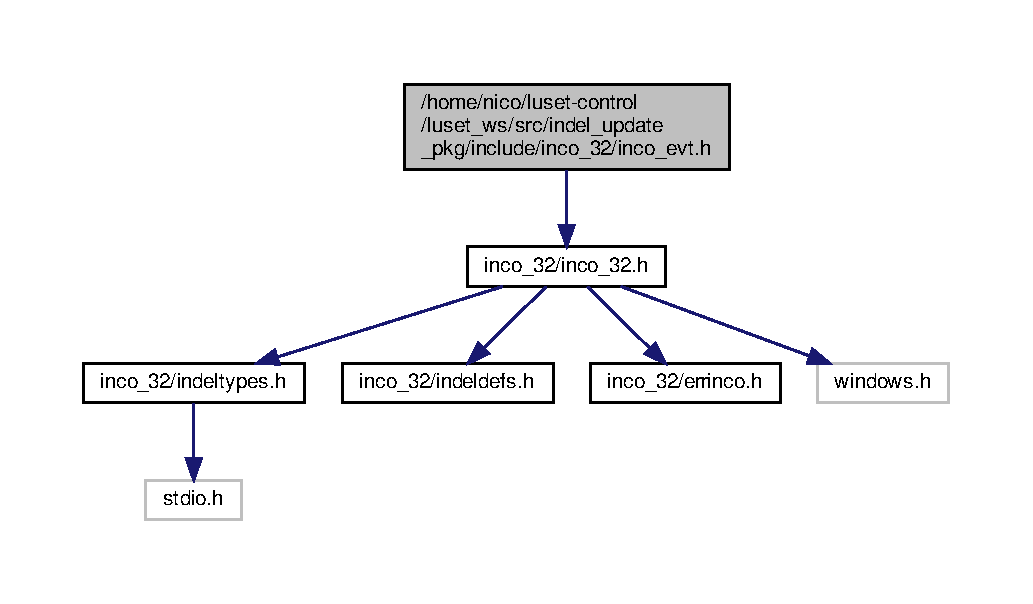
\includegraphics[width=350pt]{inco__evt_8h__incl}
\end{center}
\end{figure}
\subsection*{Macros}
\begin{DoxyCompactItemize}
\item 
\#define \hyperlink{inco__evt_8h_a69a9ff88d56a0b5c3219dc50a36cb109}{Intern\+Log}(au\+Bit\+Number,  au\+Fct\+Name,  au\+Color,  a\+Log\+Text)
\item 
\#define \hyperlink{inco__evt_8h_a6cf61a9aeb23897a55a9256639732cbd}{I\+N\+I\+X\+\_\+\+F\+A\+T\+A\+L\+E\+R\+R\+OR}(au\+Fct\+Name,  a\+Stream)
\item 
\#define \hyperlink{inco__evt_8h_acbc6e49d25287ccb9cfb7fb9ff8e096b}{I\+N\+I\+X\+\_\+\+E\+R\+R\+OR}(au\+Fct\+Name,  a\+Stream)~\hyperlink{inco__evt_8h_a69a9ff88d56a0b5c3219dc50a36cb109}{Intern\+Log}( \hyperlink{inco__evt_8h_aadb111d2e2fb704ea4ce64a670acc6e3acf549d649bed14d54f8b7e48014fb313}{e\+Error}, au\+Fct\+Name, \hyperlink{inco__evt_8h_a1b7e02f0358006e161d007c562bc887fa4521e0fa8e750c19f71f4cc88088837b}{e\+Color\+Red}, a\+Stream )
\item 
\#define \hyperlink{inco__evt_8h_a2c59b609e0a270ec336620524ac58c06}{I\+N\+I\+X\+\_\+\+W\+A\+R\+N\+I\+NG}(au\+Fct\+Name,  a\+Stream)~\hyperlink{inco__evt_8h_a69a9ff88d56a0b5c3219dc50a36cb109}{Intern\+Log}( \hyperlink{inco__evt_8h_aadb111d2e2fb704ea4ce64a670acc6e3a908397b670ff128bbed94ca4ccef13fd}{e\+Warning}, au\+Fct\+Name, \hyperlink{inco__evt_8h_a1b7e02f0358006e161d007c562bc887fa205e203eaaa2f6f777e94e66323e3d44}{e\+Color\+Yellow}, a\+Stream )
\item 
\#define \hyperlink{inco__evt_8h_afa53d6ae2c64e9321379f29e71ae1d53}{I\+N\+I\+X\+\_\+\+M\+E\+S\+S\+A\+GE}(au\+Fct\+Name,  a\+Stream)~\hyperlink{inco__evt_8h_a69a9ff88d56a0b5c3219dc50a36cb109}{Intern\+Log}( \hyperlink{inco__evt_8h_aadb111d2e2fb704ea4ce64a670acc6e3af465c6399d6e2912476078256750972b}{e\+Message}, au\+Fct\+Name, \hyperlink{inco__evt_8h_a1b7e02f0358006e161d007c562bc887fa6b23b08f002810d273b308bf620de676}{e\+Color\+Blue}, a\+Stream )
\item 
\#define \hyperlink{inco__evt_8h_aeb38d73b2fe425dd81058b4db1811550}{I\+N\+I\+X\+\_\+\+V\+E\+R\+B\+O\+SE}(au\+Fct\+Name,  a\+Stream)~\hyperlink{inco__evt_8h_a69a9ff88d56a0b5c3219dc50a36cb109}{Intern\+Log}( \hyperlink{inco__evt_8h_aadb111d2e2fb704ea4ce64a670acc6e3a2ac987b765a787bdedc9febc26216c45}{e\+Verbose}, au\+Fct\+Name, \hyperlink{inco__evt_8h_a1b7e02f0358006e161d007c562bc887faf3f63eb6d4dc4ec9c3bd2396169c137f}{e\+Color\+Std}, a\+Stream )
\item 
\#define \hyperlink{inco__evt_8h_a3992f8b7c0b0a1f98a4e40839c011f31}{I\+N\+I\+X\+\_\+\+T\+R\+A\+CE}(au\+Bit\+Number,  au\+Fct\+Name,  a\+Stream)~\hyperlink{inco__evt_8h_a69a9ff88d56a0b5c3219dc50a36cb109}{Intern\+Log}( au\+Bit\+Number, au\+Fct\+Name, \hyperlink{inco__evt_8h_a1b7e02f0358006e161d007c562bc887faf3f63eb6d4dc4ec9c3bd2396169c137f}{e\+Color\+Std}, a\+Stream )
\item 
\#define \hyperlink{inco__evt_8h_a62575c3444d6c9031ef1a9bf59f34c72}{I\+N\+I\+X\+\_\+\+F\+A\+T\+A\+L\+E\+R\+R\+O\+R\+\_\+\+C\+O\+L\+OR}(au\+Fct\+Name,  au\+Color,  a\+Stream)
\item 
\#define \hyperlink{inco__evt_8h_ab249db61d01fa3d83202fe15d8194c15}{I\+N\+I\+X\+\_\+\+E\+R\+R\+O\+R\+\_\+\+C\+O\+L\+OR}(au\+Fct\+Name,  au\+Color,  a\+Stream)~\hyperlink{inco__evt_8h_a69a9ff88d56a0b5c3219dc50a36cb109}{Intern\+Log}( \hyperlink{inco__evt_8h_aadb111d2e2fb704ea4ce64a670acc6e3acf549d649bed14d54f8b7e48014fb313}{e\+Error}, au\+Fct\+Name, au\+Color, a\+Stream )
\item 
\#define \hyperlink{inco__evt_8h_af69d58aa04ac76b2a37ec113725a0275}{I\+N\+I\+X\+\_\+\+W\+A\+R\+N\+I\+N\+G\+\_\+\+C\+O\+L\+OR}(au\+Fct\+Name,  au\+Color,  a\+Stream)~\hyperlink{inco__evt_8h_a69a9ff88d56a0b5c3219dc50a36cb109}{Intern\+Log}( \hyperlink{inco__evt_8h_aadb111d2e2fb704ea4ce64a670acc6e3a908397b670ff128bbed94ca4ccef13fd}{e\+Warning}, au\+Fct\+Name, au\+Color, a\+Stream )
\item 
\#define \hyperlink{inco__evt_8h_aedb3e5f806d41dd01a2b8614b437bdd0}{I\+N\+I\+X\+\_\+\+M\+E\+S\+S\+A\+G\+E\+\_\+\+C\+O\+L\+OR}(au\+Fct\+Name,  au\+Color,  a\+Stream)~\hyperlink{inco__evt_8h_a69a9ff88d56a0b5c3219dc50a36cb109}{Intern\+Log}( \hyperlink{inco__evt_8h_aadb111d2e2fb704ea4ce64a670acc6e3af465c6399d6e2912476078256750972b}{e\+Message}, au\+Fct\+Name, au\+Color, a\+Stream )
\item 
\#define \hyperlink{inco__evt_8h_a24975246d8c9c5153630ad29ac98c997}{I\+N\+I\+X\+\_\+\+V\+E\+R\+B\+O\+S\+E\+\_\+\+C\+O\+L\+OR}(au\+Fct\+Name,  au\+Color,  a\+Stream)~\hyperlink{inco__evt_8h_a69a9ff88d56a0b5c3219dc50a36cb109}{Intern\+Log}( \hyperlink{inco__evt_8h_aadb111d2e2fb704ea4ce64a670acc6e3a2ac987b765a787bdedc9febc26216c45}{e\+Verbose}, au\+Fct\+Name, au\+Color, a\+Stream )
\item 
\#define \hyperlink{inco__evt_8h_a51f09e08b4fa7211da086f92157ff384}{I\+N\+I\+X\+\_\+\+T\+R\+A\+C\+E\+\_\+\+C\+O\+L\+OR}(au\+Fct\+Name,  au\+Color,  au\+Bit\+Number,  a\+Stream)~\hyperlink{inco__evt_8h_a69a9ff88d56a0b5c3219dc50a36cb109}{Intern\+Log}( au\+Bit\+Number, au\+Fct\+Name, au\+Color, a\+Stream )
\end{DoxyCompactItemize}
\subsection*{Typedefs}
\begin{DoxyCompactItemize}
\item 
typedef \hyperlink{indeltypes_8h_a4b435a49c74bb91f284f075e63416cb6}{uint32}(W\+I\+N\+A\+PI $\ast$ \hyperlink{inco__evt_8h_a7f8594a700d0675b308097f8fe81fa5f}{t\+Logging\+Callback}) (\hyperlink{indeltypes_8h_a05f6b0ae8f6a6e135b0e290c25fe0e4e}{uint16} au\+Bit\+Number, const char $\ast$ap\+Fct\+Name, const char $\ast$ap\+File\+Name, \hyperlink{indeltypes_8h_a4b435a49c74bb91f284f075e63416cb6}{uint32} au\+Line\+Number, \hyperlink{indeltypes_8h_a4b435a49c74bb91f284f075e63416cb6}{uint32} au\+Font\+Color, const char $\ast$ap\+Log\+Text)
\item 
typedef \hyperlink{indeltypes_8h_a4b435a49c74bb91f284f075e63416cb6}{uint32}(W\+I\+N\+A\+PI $\ast$ \hyperlink{inco__evt_8h_ab3e62e3e192b1c44c80b9d5fc96d1623}{t\+Logging\+Level\+Callback}) (\hyperlink{indeltypes_8h_a05f6b0ae8f6a6e135b0e290c25fe0e4e}{uint16} au\+Bit\+Number)
\item 
typedef \hyperlink{indeltypes_8h_a4b435a49c74bb91f284f075e63416cb6}{uint32}(W\+I\+N\+A\+PI $\ast$ \hyperlink{inco__evt_8h_a8da5b566a61b91a51f0ef8eb02820814}{t\+Logging\+Create\+Level\+Callback}) (const char $\ast$ap\+Level\+Name, \hyperlink{indeltypes_8h_ac44d0188f4f50fd9b03031c1a06bd0a9}{int32} $\ast$ap\+Bit\+Number)
\end{DoxyCompactItemize}
\subsection*{Enumerations}
\begin{DoxyCompactItemize}
\item 
enum \hyperlink{inco__evt_8h_a1b7e02f0358006e161d007c562bc887f}{E\+Colors} \{ \newline
\hyperlink{inco__evt_8h_a1b7e02f0358006e161d007c562bc887faf3f63eb6d4dc4ec9c3bd2396169c137f}{e\+Color\+Std} = 0, 
\hyperlink{inco__evt_8h_a1b7e02f0358006e161d007c562bc887fa4521e0fa8e750c19f71f4cc88088837b}{e\+Color\+Red} = 0x000000ff, 
\hyperlink{inco__evt_8h_a1b7e02f0358006e161d007c562bc887fae33686c7364023a92b1d51275ed9f262}{e\+Color\+Green} = 0x0000c000, 
\hyperlink{inco__evt_8h_a1b7e02f0358006e161d007c562bc887fa205e203eaaa2f6f777e94e66323e3d44}{e\+Color\+Yellow} = 0x00005266, 
\newline
\hyperlink{inco__evt_8h_a1b7e02f0358006e161d007c562bc887fa6b23b08f002810d273b308bf620de676}{e\+Color\+Blue} = 0x00ff0000, 
\hyperlink{inco__evt_8h_a1b7e02f0358006e161d007c562bc887faa90369a5c20bc9867f02880f9bcaf2c0}{e\+Color\+White} = 0x00ffffff
 \}
\item 
enum \hyperlink{inco__evt_8h_aadb111d2e2fb704ea4ce64a670acc6e3}{E\+Predefined\+Log\+Levels} \{ \newline
\hyperlink{inco__evt_8h_aadb111d2e2fb704ea4ce64a670acc6e3a23e5779d5a8b76861346f484b0a458ef}{e\+Fatal\+Error} = 0, 
\hyperlink{inco__evt_8h_aadb111d2e2fb704ea4ce64a670acc6e3acf549d649bed14d54f8b7e48014fb313}{e\+Error} = 1, 
\hyperlink{inco__evt_8h_aadb111d2e2fb704ea4ce64a670acc6e3a908397b670ff128bbed94ca4ccef13fd}{e\+Warning} = 2, 
\hyperlink{inco__evt_8h_aadb111d2e2fb704ea4ce64a670acc6e3af465c6399d6e2912476078256750972b}{e\+Message} = 3, 
\newline
\hyperlink{inco__evt_8h_aadb111d2e2fb704ea4ce64a670acc6e3a2ac987b765a787bdedc9febc26216c45}{e\+Verbose} = 4, 
\hyperlink{inco__evt_8h_aadb111d2e2fb704ea4ce64a670acc6e3a799b0cbf0bd98680c28da76f27cba0fe}{e\+Server\+Frames} = 5, 
\hyperlink{inco__evt_8h_aadb111d2e2fb704ea4ce64a670acc6e3a3ec77e6a99cb1fdfd88d06fd2cf96c35}{e\+In\+Process\+Frames} = 6, 
\hyperlink{inco__evt_8h_aadb111d2e2fb704ea4ce64a670acc6e3ad0cb3cc7c3bddbd7ea2b70d1443b87d0}{e\+Call\+Procedure\+Ex} = 7, 
\newline
\hyperlink{inco__evt_8h_aadb111d2e2fb704ea4ce64a670acc6e3a43f3f0152ee32f67d8d47173c3a55079}{e\+First\+User\+Specific} = 10
 \}
\end{DoxyCompactItemize}
\subsection*{Functions}
\begin{DoxyCompactItemize}
\item 
\hyperlink{inco__32_8h_a09505cad5bbb66fc36750a4fbca0444b}{I\+N\+C\+O32\+\_\+\+E\+X\+P\+O\+RT} \hyperlink{indeltypes_8h_a4b435a49c74bb91f284f075e63416cb6}{uint32} W\+I\+N\+A\+PI \hyperlink{inco__evt_8h_ababff9314cecd98b42d12b10171154a6}{Log\+Init} (\hyperlink{inco__evt_8h_a7f8594a700d0675b308097f8fe81fa5f}{t\+Logging\+Callback} ap\+Callback, \hyperlink{inco__evt_8h_ab3e62e3e192b1c44c80b9d5fc96d1623}{t\+Logging\+Level\+Callback} ap\+Level\+Callback, \hyperlink{inco__evt_8h_a8da5b566a61b91a51f0ef8eb02820814}{t\+Logging\+Create\+Level\+Callback} ap\+Create\+Level\+Callback)
\item 
\hyperlink{inco__32_8h_a09505cad5bbb66fc36750a4fbca0444b}{I\+N\+C\+O32\+\_\+\+E\+X\+P\+O\+RT} \hyperlink{indeltypes_8h_a4b435a49c74bb91f284f075e63416cb6}{uint32} W\+I\+N\+A\+PI \hyperlink{inco__evt_8h_a8dbc6d863e95d6d40425c6dc18f749ef}{Log\+Level\+Active} (\hyperlink{indeltypes_8h_a4b435a49c74bb91f284f075e63416cb6}{uint32} au\+Bit\+Number)
\item 
\hyperlink{inco__32_8h_a09505cad5bbb66fc36750a4fbca0444b}{I\+N\+C\+O32\+\_\+\+E\+X\+P\+O\+RT} \hyperlink{indeltypes_8h_a4b435a49c74bb91f284f075e63416cb6}{uint32} W\+I\+N\+A\+PI \hyperlink{inco__evt_8h_ad77d9090ef62d3349d4bd652d469c447}{Log\+Create\+Level} (const char $\ast$ap\+Level\+Name, \hyperlink{indeltypes_8h_ac44d0188f4f50fd9b03031c1a06bd0a9}{int32} $\ast$ap\+Bit\+Number)
\item 
\hyperlink{inco__32_8h_a09505cad5bbb66fc36750a4fbca0444b}{I\+N\+C\+O32\+\_\+\+E\+X\+P\+O\+RT} \hyperlink{indeltypes_8h_a4b435a49c74bb91f284f075e63416cb6}{uint32} W\+I\+N\+A\+PI \hyperlink{inco__evt_8h_a1657a0d3b9fc2b0a9c267451a7f83577}{Log\+Message} (\hyperlink{indeltypes_8h_a05f6b0ae8f6a6e135b0e290c25fe0e4e}{uint16} au\+Bit\+Number, const char $\ast$ap\+Fct\+Name, const char $\ast$ap\+File\+Name, \hyperlink{indeltypes_8h_a4b435a49c74bb91f284f075e63416cb6}{uint32} au\+Line\+Number, \hyperlink{indeltypes_8h_a4b435a49c74bb91f284f075e63416cb6}{uint32} au\+Font\+Color, const char $\ast$ap\+Log\+Text)
\item 
\hyperlink{inco__32_8h_a09505cad5bbb66fc36750a4fbca0444b}{I\+N\+C\+O32\+\_\+\+E\+X\+P\+O\+RT} \hyperlink{indeltypes_8h_a4b435a49c74bb91f284f075e63416cb6}{uint32} W\+I\+N\+A\+PI \hyperlink{inco__evt_8h_aabc0a573051be50b3cebcfa80adc4477}{Log\+Activate\+Levels} (\hyperlink{indeltypes_8h_a05f6b0ae8f6a6e135b0e290c25fe0e4e}{uint16} au\+From, \hyperlink{indeltypes_8h_a05f6b0ae8f6a6e135b0e290c25fe0e4e}{uint16} au\+To, \hyperlink{indeltypes_8h_adde6aaee8457bee49c2a92621fe22b79}{uint8} ab\+Active)
\begin{DoxyCompactList}\small\item\em activates or deactivates specific log levels \end{DoxyCompactList}\end{DoxyCompactItemize}


\subsection{Detailed Description}
Eventlog A\+PI for inco\+\_\+32 applications. 

\begin{DoxyAuthor}{Author}
Raphael Zulliger \href{mailto:zulliger@indel.ch}{\tt zulliger@indel.\+ch}, \copyright{} I\+N\+D\+EL AG 
\end{DoxyAuthor}
\begin{DoxyVersion}{Version}
\begin{DoxyVerb}2397, 2007-12-24 16:04:14 +0100 (Mo, 24 Dez 2007), zulliger
+ Initially added the standard-Indel header to the files and thereby making
  the files icommit ready

2398, 2007-12-24 16:07:03 +0100 (Mo, 24 Dez 2007), zulliger
+ Initially added the standard-Indel header to the files and thereby making
  the files icommit ready

2447, 2008-01-29 11:45:20 +0100 (Di, 29 Jan 2008), walther
! Disable logging on Windows CE since it doesn't have <sstream>.

2618, 2008-02-27 15:46:42 +0100 (Wed, 27 Feb 2008), walther
! Set svn:eol-style property where appropriate and svn:ignore a generated
  file. [25 files]

2629, 2008-02-29 15:30:15 +0100 (Fr, 29 Feb 2008), walther
! Just noticed that I made a bit of a mess in the changelogs in r2618. Not
  sure what happened - cleaning this up...

3838, 2009-12-14 14:40:59 +0100 (Mon, 14 Dec 2009), walther
! eColorYellow, used for warnings in event logs, was hard to read on light
  backgrounds, and besides, not remotely yellow - changed.

5880, 2013-12-19 15:23:25 +0100 (Thu, 19 Dec 2013), zulliger
+ Added possibility to adjust log levels of traces generated by libinco_32
  itself by a new API call that doesn't require a callback to be installed.
  This is especially important for languages (such as .Net) for which
  calling a 'callback' for each log message is expensive.

$LastChangedRevision: 5883 $ $Date: 2013-12-20 07:46:20 +0100 (Fri, 20 Dec 2013) $ $Author: zulliger $
! Completely reworked libinco_32 tracing: The library is now using the
  INIX-trace mechanism as well (INIX_ERROR, INIX_WARNING, ...). All traces
  to stderr have been removed. Thanks to this change, INIX apps (as well as
  customer applications, such as HMIs) are easily able to get all logs
  generated by libinco_32 (such as error messages which are generated when
  async results are dropped).

$Comment$

u = unreleased
+ = new feature
! = change, bugfix
- = removed\end{DoxyVerb}

\end{DoxyVersion}
\begin{DoxyRemark}{Remarks}
\begin{DoxyVerb}project         : incoserver
language        : C++
system          : Linux, Windows - x86/PPC
\end{DoxyVerb}
 
\end{DoxyRemark}


\subsection{Macro Definition Documentation}
\mbox{\Hypertarget{inco__evt_8h_acbc6e49d25287ccb9cfb7fb9ff8e096b}\label{inco__evt_8h_acbc6e49d25287ccb9cfb7fb9ff8e096b}} 
\index{inco\+\_\+evt.\+h@{inco\+\_\+evt.\+h}!I\+N\+I\+X\+\_\+\+E\+R\+R\+OR@{I\+N\+I\+X\+\_\+\+E\+R\+R\+OR}}
\index{I\+N\+I\+X\+\_\+\+E\+R\+R\+OR@{I\+N\+I\+X\+\_\+\+E\+R\+R\+OR}!inco\+\_\+evt.\+h@{inco\+\_\+evt.\+h}}
\subsubsection{\texorpdfstring{I\+N\+I\+X\+\_\+\+E\+R\+R\+OR}{INIX\_ERROR}}
{\footnotesize\ttfamily \#define I\+N\+I\+X\+\_\+\+E\+R\+R\+OR(\begin{DoxyParamCaption}\item[{}]{au\+Fct\+Name,  }\item[{}]{a\+Stream }\end{DoxyParamCaption})~\hyperlink{inco__evt_8h_a69a9ff88d56a0b5c3219dc50a36cb109}{Intern\+Log}( \hyperlink{inco__evt_8h_aadb111d2e2fb704ea4ce64a670acc6e3acf549d649bed14d54f8b7e48014fb313}{e\+Error}, au\+Fct\+Name, \hyperlink{inco__evt_8h_a1b7e02f0358006e161d007c562bc887fa4521e0fa8e750c19f71f4cc88088837b}{e\+Color\+Red}, a\+Stream )}

\mbox{\Hypertarget{inco__evt_8h_ab249db61d01fa3d83202fe15d8194c15}\label{inco__evt_8h_ab249db61d01fa3d83202fe15d8194c15}} 
\index{inco\+\_\+evt.\+h@{inco\+\_\+evt.\+h}!I\+N\+I\+X\+\_\+\+E\+R\+R\+O\+R\+\_\+\+C\+O\+L\+OR@{I\+N\+I\+X\+\_\+\+E\+R\+R\+O\+R\+\_\+\+C\+O\+L\+OR}}
\index{I\+N\+I\+X\+\_\+\+E\+R\+R\+O\+R\+\_\+\+C\+O\+L\+OR@{I\+N\+I\+X\+\_\+\+E\+R\+R\+O\+R\+\_\+\+C\+O\+L\+OR}!inco\+\_\+evt.\+h@{inco\+\_\+evt.\+h}}
\subsubsection{\texorpdfstring{I\+N\+I\+X\+\_\+\+E\+R\+R\+O\+R\+\_\+\+C\+O\+L\+OR}{INIX\_ERROR\_COLOR}}
{\footnotesize\ttfamily \#define I\+N\+I\+X\+\_\+\+E\+R\+R\+O\+R\+\_\+\+C\+O\+L\+OR(\begin{DoxyParamCaption}\item[{}]{au\+Fct\+Name,  }\item[{}]{au\+Color,  }\item[{}]{a\+Stream }\end{DoxyParamCaption})~\hyperlink{inco__evt_8h_a69a9ff88d56a0b5c3219dc50a36cb109}{Intern\+Log}( \hyperlink{inco__evt_8h_aadb111d2e2fb704ea4ce64a670acc6e3acf549d649bed14d54f8b7e48014fb313}{e\+Error}, au\+Fct\+Name, au\+Color, a\+Stream )}

\mbox{\Hypertarget{inco__evt_8h_a6cf61a9aeb23897a55a9256639732cbd}\label{inco__evt_8h_a6cf61a9aeb23897a55a9256639732cbd}} 
\index{inco\+\_\+evt.\+h@{inco\+\_\+evt.\+h}!I\+N\+I\+X\+\_\+\+F\+A\+T\+A\+L\+E\+R\+R\+OR@{I\+N\+I\+X\+\_\+\+F\+A\+T\+A\+L\+E\+R\+R\+OR}}
\index{I\+N\+I\+X\+\_\+\+F\+A\+T\+A\+L\+E\+R\+R\+OR@{I\+N\+I\+X\+\_\+\+F\+A\+T\+A\+L\+E\+R\+R\+OR}!inco\+\_\+evt.\+h@{inco\+\_\+evt.\+h}}
\subsubsection{\texorpdfstring{I\+N\+I\+X\+\_\+\+F\+A\+T\+A\+L\+E\+R\+R\+OR}{INIX\_FATALERROR}}
{\footnotesize\ttfamily \#define I\+N\+I\+X\+\_\+\+F\+A\+T\+A\+L\+E\+R\+R\+OR(\begin{DoxyParamCaption}\item[{}]{au\+Fct\+Name,  }\item[{}]{a\+Stream }\end{DoxyParamCaption})}

{\bfseries Value\+:}
\begin{DoxyCode}
\hyperlink{inco__evt_8h_a69a9ff88d56a0b5c3219dc50a36cb109}{InternLog}( \hyperlink{inco__evt_8h_aadb111d2e2fb704ea4ce64a670acc6e3a23e5779d5a8b76861346f484b0a458ef}{eFatalError}, auFctName, \hyperlink{inco__evt_8h_a1b7e02f0358006e161d007c562bc887fa4521e0fa8e750c19f71f4cc88088837b}{eColorRed}, aStream ) \(\backslash\)
    wxASSERT(0)
\end{DoxyCode}
\mbox{\Hypertarget{inco__evt_8h_a62575c3444d6c9031ef1a9bf59f34c72}\label{inco__evt_8h_a62575c3444d6c9031ef1a9bf59f34c72}} 
\index{inco\+\_\+evt.\+h@{inco\+\_\+evt.\+h}!I\+N\+I\+X\+\_\+\+F\+A\+T\+A\+L\+E\+R\+R\+O\+R\+\_\+\+C\+O\+L\+OR@{I\+N\+I\+X\+\_\+\+F\+A\+T\+A\+L\+E\+R\+R\+O\+R\+\_\+\+C\+O\+L\+OR}}
\index{I\+N\+I\+X\+\_\+\+F\+A\+T\+A\+L\+E\+R\+R\+O\+R\+\_\+\+C\+O\+L\+OR@{I\+N\+I\+X\+\_\+\+F\+A\+T\+A\+L\+E\+R\+R\+O\+R\+\_\+\+C\+O\+L\+OR}!inco\+\_\+evt.\+h@{inco\+\_\+evt.\+h}}
\subsubsection{\texorpdfstring{I\+N\+I\+X\+\_\+\+F\+A\+T\+A\+L\+E\+R\+R\+O\+R\+\_\+\+C\+O\+L\+OR}{INIX\_FATALERROR\_COLOR}}
{\footnotesize\ttfamily \#define I\+N\+I\+X\+\_\+\+F\+A\+T\+A\+L\+E\+R\+R\+O\+R\+\_\+\+C\+O\+L\+OR(\begin{DoxyParamCaption}\item[{}]{au\+Fct\+Name,  }\item[{}]{au\+Color,  }\item[{}]{a\+Stream }\end{DoxyParamCaption})}

{\bfseries Value\+:}
\begin{DoxyCode}
\hyperlink{inco__evt_8h_a69a9ff88d56a0b5c3219dc50a36cb109}{InternLog}( \hyperlink{inco__evt_8h_aadb111d2e2fb704ea4ce64a670acc6e3a23e5779d5a8b76861346f484b0a458ef}{eFatalError}, auFctName, auColor,  \(\backslash\)
            aStream ) \(\backslash\)
    wxASSERT(0)
\end{DoxyCode}
\mbox{\Hypertarget{inco__evt_8h_afa53d6ae2c64e9321379f29e71ae1d53}\label{inco__evt_8h_afa53d6ae2c64e9321379f29e71ae1d53}} 
\index{inco\+\_\+evt.\+h@{inco\+\_\+evt.\+h}!I\+N\+I\+X\+\_\+\+M\+E\+S\+S\+A\+GE@{I\+N\+I\+X\+\_\+\+M\+E\+S\+S\+A\+GE}}
\index{I\+N\+I\+X\+\_\+\+M\+E\+S\+S\+A\+GE@{I\+N\+I\+X\+\_\+\+M\+E\+S\+S\+A\+GE}!inco\+\_\+evt.\+h@{inco\+\_\+evt.\+h}}
\subsubsection{\texorpdfstring{I\+N\+I\+X\+\_\+\+M\+E\+S\+S\+A\+GE}{INIX\_MESSAGE}}
{\footnotesize\ttfamily \#define I\+N\+I\+X\+\_\+\+M\+E\+S\+S\+A\+GE(\begin{DoxyParamCaption}\item[{}]{au\+Fct\+Name,  }\item[{}]{a\+Stream }\end{DoxyParamCaption})~\hyperlink{inco__evt_8h_a69a9ff88d56a0b5c3219dc50a36cb109}{Intern\+Log}( \hyperlink{inco__evt_8h_aadb111d2e2fb704ea4ce64a670acc6e3af465c6399d6e2912476078256750972b}{e\+Message}, au\+Fct\+Name, \hyperlink{inco__evt_8h_a1b7e02f0358006e161d007c562bc887fa6b23b08f002810d273b308bf620de676}{e\+Color\+Blue}, a\+Stream )}

\mbox{\Hypertarget{inco__evt_8h_aedb3e5f806d41dd01a2b8614b437bdd0}\label{inco__evt_8h_aedb3e5f806d41dd01a2b8614b437bdd0}} 
\index{inco\+\_\+evt.\+h@{inco\+\_\+evt.\+h}!I\+N\+I\+X\+\_\+\+M\+E\+S\+S\+A\+G\+E\+\_\+\+C\+O\+L\+OR@{I\+N\+I\+X\+\_\+\+M\+E\+S\+S\+A\+G\+E\+\_\+\+C\+O\+L\+OR}}
\index{I\+N\+I\+X\+\_\+\+M\+E\+S\+S\+A\+G\+E\+\_\+\+C\+O\+L\+OR@{I\+N\+I\+X\+\_\+\+M\+E\+S\+S\+A\+G\+E\+\_\+\+C\+O\+L\+OR}!inco\+\_\+evt.\+h@{inco\+\_\+evt.\+h}}
\subsubsection{\texorpdfstring{I\+N\+I\+X\+\_\+\+M\+E\+S\+S\+A\+G\+E\+\_\+\+C\+O\+L\+OR}{INIX\_MESSAGE\_COLOR}}
{\footnotesize\ttfamily \#define I\+N\+I\+X\+\_\+\+M\+E\+S\+S\+A\+G\+E\+\_\+\+C\+O\+L\+OR(\begin{DoxyParamCaption}\item[{}]{au\+Fct\+Name,  }\item[{}]{au\+Color,  }\item[{}]{a\+Stream }\end{DoxyParamCaption})~\hyperlink{inco__evt_8h_a69a9ff88d56a0b5c3219dc50a36cb109}{Intern\+Log}( \hyperlink{inco__evt_8h_aadb111d2e2fb704ea4ce64a670acc6e3af465c6399d6e2912476078256750972b}{e\+Message}, au\+Fct\+Name, au\+Color, a\+Stream )}

\mbox{\Hypertarget{inco__evt_8h_a3992f8b7c0b0a1f98a4e40839c011f31}\label{inco__evt_8h_a3992f8b7c0b0a1f98a4e40839c011f31}} 
\index{inco\+\_\+evt.\+h@{inco\+\_\+evt.\+h}!I\+N\+I\+X\+\_\+\+T\+R\+A\+CE@{I\+N\+I\+X\+\_\+\+T\+R\+A\+CE}}
\index{I\+N\+I\+X\+\_\+\+T\+R\+A\+CE@{I\+N\+I\+X\+\_\+\+T\+R\+A\+CE}!inco\+\_\+evt.\+h@{inco\+\_\+evt.\+h}}
\subsubsection{\texorpdfstring{I\+N\+I\+X\+\_\+\+T\+R\+A\+CE}{INIX\_TRACE}}
{\footnotesize\ttfamily \#define I\+N\+I\+X\+\_\+\+T\+R\+A\+CE(\begin{DoxyParamCaption}\item[{}]{au\+Bit\+Number,  }\item[{}]{au\+Fct\+Name,  }\item[{}]{a\+Stream }\end{DoxyParamCaption})~\hyperlink{inco__evt_8h_a69a9ff88d56a0b5c3219dc50a36cb109}{Intern\+Log}( au\+Bit\+Number, au\+Fct\+Name, \hyperlink{inco__evt_8h_a1b7e02f0358006e161d007c562bc887faf3f63eb6d4dc4ec9c3bd2396169c137f}{e\+Color\+Std}, a\+Stream )}

\mbox{\Hypertarget{inco__evt_8h_a51f09e08b4fa7211da086f92157ff384}\label{inco__evt_8h_a51f09e08b4fa7211da086f92157ff384}} 
\index{inco\+\_\+evt.\+h@{inco\+\_\+evt.\+h}!I\+N\+I\+X\+\_\+\+T\+R\+A\+C\+E\+\_\+\+C\+O\+L\+OR@{I\+N\+I\+X\+\_\+\+T\+R\+A\+C\+E\+\_\+\+C\+O\+L\+OR}}
\index{I\+N\+I\+X\+\_\+\+T\+R\+A\+C\+E\+\_\+\+C\+O\+L\+OR@{I\+N\+I\+X\+\_\+\+T\+R\+A\+C\+E\+\_\+\+C\+O\+L\+OR}!inco\+\_\+evt.\+h@{inco\+\_\+evt.\+h}}
\subsubsection{\texorpdfstring{I\+N\+I\+X\+\_\+\+T\+R\+A\+C\+E\+\_\+\+C\+O\+L\+OR}{INIX\_TRACE\_COLOR}}
{\footnotesize\ttfamily \#define I\+N\+I\+X\+\_\+\+T\+R\+A\+C\+E\+\_\+\+C\+O\+L\+OR(\begin{DoxyParamCaption}\item[{}]{au\+Fct\+Name,  }\item[{}]{au\+Color,  }\item[{}]{au\+Bit\+Number,  }\item[{}]{a\+Stream }\end{DoxyParamCaption})~\hyperlink{inco__evt_8h_a69a9ff88d56a0b5c3219dc50a36cb109}{Intern\+Log}( au\+Bit\+Number, au\+Fct\+Name, au\+Color, a\+Stream )}

\mbox{\Hypertarget{inco__evt_8h_aeb38d73b2fe425dd81058b4db1811550}\label{inco__evt_8h_aeb38d73b2fe425dd81058b4db1811550}} 
\index{inco\+\_\+evt.\+h@{inco\+\_\+evt.\+h}!I\+N\+I\+X\+\_\+\+V\+E\+R\+B\+O\+SE@{I\+N\+I\+X\+\_\+\+V\+E\+R\+B\+O\+SE}}
\index{I\+N\+I\+X\+\_\+\+V\+E\+R\+B\+O\+SE@{I\+N\+I\+X\+\_\+\+V\+E\+R\+B\+O\+SE}!inco\+\_\+evt.\+h@{inco\+\_\+evt.\+h}}
\subsubsection{\texorpdfstring{I\+N\+I\+X\+\_\+\+V\+E\+R\+B\+O\+SE}{INIX\_VERBOSE}}
{\footnotesize\ttfamily \#define I\+N\+I\+X\+\_\+\+V\+E\+R\+B\+O\+SE(\begin{DoxyParamCaption}\item[{}]{au\+Fct\+Name,  }\item[{}]{a\+Stream }\end{DoxyParamCaption})~\hyperlink{inco__evt_8h_a69a9ff88d56a0b5c3219dc50a36cb109}{Intern\+Log}( \hyperlink{inco__evt_8h_aadb111d2e2fb704ea4ce64a670acc6e3a2ac987b765a787bdedc9febc26216c45}{e\+Verbose}, au\+Fct\+Name, \hyperlink{inco__evt_8h_a1b7e02f0358006e161d007c562bc887faf3f63eb6d4dc4ec9c3bd2396169c137f}{e\+Color\+Std}, a\+Stream )}

\mbox{\Hypertarget{inco__evt_8h_a24975246d8c9c5153630ad29ac98c997}\label{inco__evt_8h_a24975246d8c9c5153630ad29ac98c997}} 
\index{inco\+\_\+evt.\+h@{inco\+\_\+evt.\+h}!I\+N\+I\+X\+\_\+\+V\+E\+R\+B\+O\+S\+E\+\_\+\+C\+O\+L\+OR@{I\+N\+I\+X\+\_\+\+V\+E\+R\+B\+O\+S\+E\+\_\+\+C\+O\+L\+OR}}
\index{I\+N\+I\+X\+\_\+\+V\+E\+R\+B\+O\+S\+E\+\_\+\+C\+O\+L\+OR@{I\+N\+I\+X\+\_\+\+V\+E\+R\+B\+O\+S\+E\+\_\+\+C\+O\+L\+OR}!inco\+\_\+evt.\+h@{inco\+\_\+evt.\+h}}
\subsubsection{\texorpdfstring{I\+N\+I\+X\+\_\+\+V\+E\+R\+B\+O\+S\+E\+\_\+\+C\+O\+L\+OR}{INIX\_VERBOSE\_COLOR}}
{\footnotesize\ttfamily \#define I\+N\+I\+X\+\_\+\+V\+E\+R\+B\+O\+S\+E\+\_\+\+C\+O\+L\+OR(\begin{DoxyParamCaption}\item[{}]{au\+Fct\+Name,  }\item[{}]{au\+Color,  }\item[{}]{a\+Stream }\end{DoxyParamCaption})~\hyperlink{inco__evt_8h_a69a9ff88d56a0b5c3219dc50a36cb109}{Intern\+Log}( \hyperlink{inco__evt_8h_aadb111d2e2fb704ea4ce64a670acc6e3a2ac987b765a787bdedc9febc26216c45}{e\+Verbose}, au\+Fct\+Name, au\+Color, a\+Stream )}

\mbox{\Hypertarget{inco__evt_8h_a2c59b609e0a270ec336620524ac58c06}\label{inco__evt_8h_a2c59b609e0a270ec336620524ac58c06}} 
\index{inco\+\_\+evt.\+h@{inco\+\_\+evt.\+h}!I\+N\+I\+X\+\_\+\+W\+A\+R\+N\+I\+NG@{I\+N\+I\+X\+\_\+\+W\+A\+R\+N\+I\+NG}}
\index{I\+N\+I\+X\+\_\+\+W\+A\+R\+N\+I\+NG@{I\+N\+I\+X\+\_\+\+W\+A\+R\+N\+I\+NG}!inco\+\_\+evt.\+h@{inco\+\_\+evt.\+h}}
\subsubsection{\texorpdfstring{I\+N\+I\+X\+\_\+\+W\+A\+R\+N\+I\+NG}{INIX\_WARNING}}
{\footnotesize\ttfamily \#define I\+N\+I\+X\+\_\+\+W\+A\+R\+N\+I\+NG(\begin{DoxyParamCaption}\item[{}]{au\+Fct\+Name,  }\item[{}]{a\+Stream }\end{DoxyParamCaption})~\hyperlink{inco__evt_8h_a69a9ff88d56a0b5c3219dc50a36cb109}{Intern\+Log}( \hyperlink{inco__evt_8h_aadb111d2e2fb704ea4ce64a670acc6e3a908397b670ff128bbed94ca4ccef13fd}{e\+Warning}, au\+Fct\+Name, \hyperlink{inco__evt_8h_a1b7e02f0358006e161d007c562bc887fa205e203eaaa2f6f777e94e66323e3d44}{e\+Color\+Yellow}, a\+Stream )}

\mbox{\Hypertarget{inco__evt_8h_af69d58aa04ac76b2a37ec113725a0275}\label{inco__evt_8h_af69d58aa04ac76b2a37ec113725a0275}} 
\index{inco\+\_\+evt.\+h@{inco\+\_\+evt.\+h}!I\+N\+I\+X\+\_\+\+W\+A\+R\+N\+I\+N\+G\+\_\+\+C\+O\+L\+OR@{I\+N\+I\+X\+\_\+\+W\+A\+R\+N\+I\+N\+G\+\_\+\+C\+O\+L\+OR}}
\index{I\+N\+I\+X\+\_\+\+W\+A\+R\+N\+I\+N\+G\+\_\+\+C\+O\+L\+OR@{I\+N\+I\+X\+\_\+\+W\+A\+R\+N\+I\+N\+G\+\_\+\+C\+O\+L\+OR}!inco\+\_\+evt.\+h@{inco\+\_\+evt.\+h}}
\subsubsection{\texorpdfstring{I\+N\+I\+X\+\_\+\+W\+A\+R\+N\+I\+N\+G\+\_\+\+C\+O\+L\+OR}{INIX\_WARNING\_COLOR}}
{\footnotesize\ttfamily \#define I\+N\+I\+X\+\_\+\+W\+A\+R\+N\+I\+N\+G\+\_\+\+C\+O\+L\+OR(\begin{DoxyParamCaption}\item[{}]{au\+Fct\+Name,  }\item[{}]{au\+Color,  }\item[{}]{a\+Stream }\end{DoxyParamCaption})~\hyperlink{inco__evt_8h_a69a9ff88d56a0b5c3219dc50a36cb109}{Intern\+Log}( \hyperlink{inco__evt_8h_aadb111d2e2fb704ea4ce64a670acc6e3a908397b670ff128bbed94ca4ccef13fd}{e\+Warning}, au\+Fct\+Name, au\+Color, a\+Stream )}

\mbox{\Hypertarget{inco__evt_8h_a69a9ff88d56a0b5c3219dc50a36cb109}\label{inco__evt_8h_a69a9ff88d56a0b5c3219dc50a36cb109}} 
\index{inco\+\_\+evt.\+h@{inco\+\_\+evt.\+h}!Intern\+Log@{Intern\+Log}}
\index{Intern\+Log@{Intern\+Log}!inco\+\_\+evt.\+h@{inco\+\_\+evt.\+h}}
\subsubsection{\texorpdfstring{Intern\+Log}{InternLog}}
{\footnotesize\ttfamily \#define Intern\+Log(\begin{DoxyParamCaption}\item[{}]{au\+Bit\+Number,  }\item[{}]{au\+Fct\+Name,  }\item[{}]{au\+Color,  }\item[{}]{a\+Log\+Text }\end{DoxyParamCaption})}

{\bfseries Value\+:}
\begin{DoxyCode}
\textcolor{keywordflow}{if}( \hyperlink{inco__evt_8h_a8dbc6d863e95d6d40425c6dc18f749ef}{LogLevelActive}(auBitNumber) == 
      \hyperlink{errinco_8h_a6a9b824e853028ed31684c34faef6773}{DF\_ER\_INIX\_LOGGER\_LEVEL\_IS\_ACTIVE} ) \(\backslash\)
        \{ \(\backslash\)
            do \(\backslash\)
            \{ \(\backslash\)
                using \textcolor{keyword}{namespace }std; \(\backslash\)
                ostringstream Text; \(\backslash\)
                Text << aLogText; \(\backslash\)
                LogMessage( auBitNumber, \(\backslash\)
                auFctName, \(\backslash\)
                \_\_FILE\_\_, \(\backslash\)
                \_\_LINE\_\_, \(\backslash\)
                auColor, \(\backslash\)
                Text.str().c\_str() ); \(\backslash\)
            \} \textcolor{keywordflow}{while}(0); \(\backslash\)
        \}
\end{DoxyCode}


\subsection{Typedef Documentation}
\mbox{\Hypertarget{inco__evt_8h_a7f8594a700d0675b308097f8fe81fa5f}\label{inco__evt_8h_a7f8594a700d0675b308097f8fe81fa5f}} 
\index{inco\+\_\+evt.\+h@{inco\+\_\+evt.\+h}!t\+Logging\+Callback@{t\+Logging\+Callback}}
\index{t\+Logging\+Callback@{t\+Logging\+Callback}!inco\+\_\+evt.\+h@{inco\+\_\+evt.\+h}}
\subsubsection{\texorpdfstring{t\+Logging\+Callback}{tLoggingCallback}}
{\footnotesize\ttfamily typedef \hyperlink{indeltypes_8h_a4b435a49c74bb91f284f075e63416cb6}{uint32}(W\+I\+N\+A\+PI $\ast$ t\+Logging\+Callback) (\hyperlink{indeltypes_8h_a05f6b0ae8f6a6e135b0e290c25fe0e4e}{uint16} au\+Bit\+Number, const char $\ast$ap\+Fct\+Name, const char $\ast$ap\+File\+Name, \hyperlink{indeltypes_8h_a4b435a49c74bb91f284f075e63416cb6}{uint32} au\+Line\+Number, \hyperlink{indeltypes_8h_a4b435a49c74bb91f284f075e63416cb6}{uint32} au\+Font\+Color, const char $\ast$ap\+Log\+Text)}

\mbox{\Hypertarget{inco__evt_8h_a8da5b566a61b91a51f0ef8eb02820814}\label{inco__evt_8h_a8da5b566a61b91a51f0ef8eb02820814}} 
\index{inco\+\_\+evt.\+h@{inco\+\_\+evt.\+h}!t\+Logging\+Create\+Level\+Callback@{t\+Logging\+Create\+Level\+Callback}}
\index{t\+Logging\+Create\+Level\+Callback@{t\+Logging\+Create\+Level\+Callback}!inco\+\_\+evt.\+h@{inco\+\_\+evt.\+h}}
\subsubsection{\texorpdfstring{t\+Logging\+Create\+Level\+Callback}{tLoggingCreateLevelCallback}}
{\footnotesize\ttfamily typedef \hyperlink{indeltypes_8h_a4b435a49c74bb91f284f075e63416cb6}{uint32}(W\+I\+N\+A\+PI $\ast$ t\+Logging\+Create\+Level\+Callback) (const char $\ast$ap\+Level\+Name, \hyperlink{indeltypes_8h_ac44d0188f4f50fd9b03031c1a06bd0a9}{int32} $\ast$ap\+Bit\+Number)}

\mbox{\Hypertarget{inco__evt_8h_ab3e62e3e192b1c44c80b9d5fc96d1623}\label{inco__evt_8h_ab3e62e3e192b1c44c80b9d5fc96d1623}} 
\index{inco\+\_\+evt.\+h@{inco\+\_\+evt.\+h}!t\+Logging\+Level\+Callback@{t\+Logging\+Level\+Callback}}
\index{t\+Logging\+Level\+Callback@{t\+Logging\+Level\+Callback}!inco\+\_\+evt.\+h@{inco\+\_\+evt.\+h}}
\subsubsection{\texorpdfstring{t\+Logging\+Level\+Callback}{tLoggingLevelCallback}}
{\footnotesize\ttfamily typedef \hyperlink{indeltypes_8h_a4b435a49c74bb91f284f075e63416cb6}{uint32}(W\+I\+N\+A\+PI $\ast$ t\+Logging\+Level\+Callback) (\hyperlink{indeltypes_8h_a05f6b0ae8f6a6e135b0e290c25fe0e4e}{uint16} au\+Bit\+Number)}



\subsection{Enumeration Type Documentation}
\mbox{\Hypertarget{inco__evt_8h_a1b7e02f0358006e161d007c562bc887f}\label{inco__evt_8h_a1b7e02f0358006e161d007c562bc887f}} 
\index{inco\+\_\+evt.\+h@{inco\+\_\+evt.\+h}!E\+Colors@{E\+Colors}}
\index{E\+Colors@{E\+Colors}!inco\+\_\+evt.\+h@{inco\+\_\+evt.\+h}}
\subsubsection{\texorpdfstring{E\+Colors}{EColors}}
{\footnotesize\ttfamily enum \hyperlink{inco__evt_8h_a1b7e02f0358006e161d007c562bc887f}{E\+Colors}}

\begin{DoxyEnumFields}{Enumerator}
\raisebox{\heightof{T}}[0pt][0pt]{\index{e\+Color\+Std@{e\+Color\+Std}!inco\+\_\+evt.\+h@{inco\+\_\+evt.\+h}}\index{inco\+\_\+evt.\+h@{inco\+\_\+evt.\+h}!e\+Color\+Std@{e\+Color\+Std}}}\mbox{\Hypertarget{inco__evt_8h_a1b7e02f0358006e161d007c562bc887faf3f63eb6d4dc4ec9c3bd2396169c137f}\label{inco__evt_8h_a1b7e02f0358006e161d007c562bc887faf3f63eb6d4dc4ec9c3bd2396169c137f}} 
e\+Color\+Std&\\
\hline

\raisebox{\heightof{T}}[0pt][0pt]{\index{e\+Color\+Red@{e\+Color\+Red}!inco\+\_\+evt.\+h@{inco\+\_\+evt.\+h}}\index{inco\+\_\+evt.\+h@{inco\+\_\+evt.\+h}!e\+Color\+Red@{e\+Color\+Red}}}\mbox{\Hypertarget{inco__evt_8h_a1b7e02f0358006e161d007c562bc887fa4521e0fa8e750c19f71f4cc88088837b}\label{inco__evt_8h_a1b7e02f0358006e161d007c562bc887fa4521e0fa8e750c19f71f4cc88088837b}} 
e\+Color\+Red&\\
\hline

\raisebox{\heightof{T}}[0pt][0pt]{\index{e\+Color\+Green@{e\+Color\+Green}!inco\+\_\+evt.\+h@{inco\+\_\+evt.\+h}}\index{inco\+\_\+evt.\+h@{inco\+\_\+evt.\+h}!e\+Color\+Green@{e\+Color\+Green}}}\mbox{\Hypertarget{inco__evt_8h_a1b7e02f0358006e161d007c562bc887fae33686c7364023a92b1d51275ed9f262}\label{inco__evt_8h_a1b7e02f0358006e161d007c562bc887fae33686c7364023a92b1d51275ed9f262}} 
e\+Color\+Green&\\
\hline

\raisebox{\heightof{T}}[0pt][0pt]{\index{e\+Color\+Yellow@{e\+Color\+Yellow}!inco\+\_\+evt.\+h@{inco\+\_\+evt.\+h}}\index{inco\+\_\+evt.\+h@{inco\+\_\+evt.\+h}!e\+Color\+Yellow@{e\+Color\+Yellow}}}\mbox{\Hypertarget{inco__evt_8h_a1b7e02f0358006e161d007c562bc887fa205e203eaaa2f6f777e94e66323e3d44}\label{inco__evt_8h_a1b7e02f0358006e161d007c562bc887fa205e203eaaa2f6f777e94e66323e3d44}} 
e\+Color\+Yellow&\\
\hline

\raisebox{\heightof{T}}[0pt][0pt]{\index{e\+Color\+Blue@{e\+Color\+Blue}!inco\+\_\+evt.\+h@{inco\+\_\+evt.\+h}}\index{inco\+\_\+evt.\+h@{inco\+\_\+evt.\+h}!e\+Color\+Blue@{e\+Color\+Blue}}}\mbox{\Hypertarget{inco__evt_8h_a1b7e02f0358006e161d007c562bc887fa6b23b08f002810d273b308bf620de676}\label{inco__evt_8h_a1b7e02f0358006e161d007c562bc887fa6b23b08f002810d273b308bf620de676}} 
e\+Color\+Blue&\\
\hline

\raisebox{\heightof{T}}[0pt][0pt]{\index{e\+Color\+White@{e\+Color\+White}!inco\+\_\+evt.\+h@{inco\+\_\+evt.\+h}}\index{inco\+\_\+evt.\+h@{inco\+\_\+evt.\+h}!e\+Color\+White@{e\+Color\+White}}}\mbox{\Hypertarget{inco__evt_8h_a1b7e02f0358006e161d007c562bc887faa90369a5c20bc9867f02880f9bcaf2c0}\label{inco__evt_8h_a1b7e02f0358006e161d007c562bc887faa90369a5c20bc9867f02880f9bcaf2c0}} 
e\+Color\+White&\\
\hline

\end{DoxyEnumFields}
\mbox{\Hypertarget{inco__evt_8h_aadb111d2e2fb704ea4ce64a670acc6e3}\label{inco__evt_8h_aadb111d2e2fb704ea4ce64a670acc6e3}} 
\index{inco\+\_\+evt.\+h@{inco\+\_\+evt.\+h}!E\+Predefined\+Log\+Levels@{E\+Predefined\+Log\+Levels}}
\index{E\+Predefined\+Log\+Levels@{E\+Predefined\+Log\+Levels}!inco\+\_\+evt.\+h@{inco\+\_\+evt.\+h}}
\subsubsection{\texorpdfstring{E\+Predefined\+Log\+Levels}{EPredefinedLogLevels}}
{\footnotesize\ttfamily enum \hyperlink{inco__evt_8h_aadb111d2e2fb704ea4ce64a670acc6e3}{E\+Predefined\+Log\+Levels}}

\begin{DoxyEnumFields}{Enumerator}
\raisebox{\heightof{T}}[0pt][0pt]{\index{e\+Fatal\+Error@{e\+Fatal\+Error}!inco\+\_\+evt.\+h@{inco\+\_\+evt.\+h}}\index{inco\+\_\+evt.\+h@{inco\+\_\+evt.\+h}!e\+Fatal\+Error@{e\+Fatal\+Error}}}\mbox{\Hypertarget{inco__evt_8h_aadb111d2e2fb704ea4ce64a670acc6e3a23e5779d5a8b76861346f484b0a458ef}\label{inco__evt_8h_aadb111d2e2fb704ea4ce64a670acc6e3a23e5779d5a8b76861346f484b0a458ef}} 
e\+Fatal\+Error&\\
\hline

\raisebox{\heightof{T}}[0pt][0pt]{\index{e\+Error@{e\+Error}!inco\+\_\+evt.\+h@{inco\+\_\+evt.\+h}}\index{inco\+\_\+evt.\+h@{inco\+\_\+evt.\+h}!e\+Error@{e\+Error}}}\mbox{\Hypertarget{inco__evt_8h_aadb111d2e2fb704ea4ce64a670acc6e3acf549d649bed14d54f8b7e48014fb313}\label{inco__evt_8h_aadb111d2e2fb704ea4ce64a670acc6e3acf549d649bed14d54f8b7e48014fb313}} 
e\+Error&\\
\hline

\raisebox{\heightof{T}}[0pt][0pt]{\index{e\+Warning@{e\+Warning}!inco\+\_\+evt.\+h@{inco\+\_\+evt.\+h}}\index{inco\+\_\+evt.\+h@{inco\+\_\+evt.\+h}!e\+Warning@{e\+Warning}}}\mbox{\Hypertarget{inco__evt_8h_aadb111d2e2fb704ea4ce64a670acc6e3a908397b670ff128bbed94ca4ccef13fd}\label{inco__evt_8h_aadb111d2e2fb704ea4ce64a670acc6e3a908397b670ff128bbed94ca4ccef13fd}} 
e\+Warning&\\
\hline

\raisebox{\heightof{T}}[0pt][0pt]{\index{e\+Message@{e\+Message}!inco\+\_\+evt.\+h@{inco\+\_\+evt.\+h}}\index{inco\+\_\+evt.\+h@{inco\+\_\+evt.\+h}!e\+Message@{e\+Message}}}\mbox{\Hypertarget{inco__evt_8h_aadb111d2e2fb704ea4ce64a670acc6e3af465c6399d6e2912476078256750972b}\label{inco__evt_8h_aadb111d2e2fb704ea4ce64a670acc6e3af465c6399d6e2912476078256750972b}} 
e\+Message&\\
\hline

\raisebox{\heightof{T}}[0pt][0pt]{\index{e\+Verbose@{e\+Verbose}!inco\+\_\+evt.\+h@{inco\+\_\+evt.\+h}}\index{inco\+\_\+evt.\+h@{inco\+\_\+evt.\+h}!e\+Verbose@{e\+Verbose}}}\mbox{\Hypertarget{inco__evt_8h_aadb111d2e2fb704ea4ce64a670acc6e3a2ac987b765a787bdedc9febc26216c45}\label{inco__evt_8h_aadb111d2e2fb704ea4ce64a670acc6e3a2ac987b765a787bdedc9febc26216c45}} 
e\+Verbose&\\
\hline

\raisebox{\heightof{T}}[0pt][0pt]{\index{e\+Server\+Frames@{e\+Server\+Frames}!inco\+\_\+evt.\+h@{inco\+\_\+evt.\+h}}\index{inco\+\_\+evt.\+h@{inco\+\_\+evt.\+h}!e\+Server\+Frames@{e\+Server\+Frames}}}\mbox{\Hypertarget{inco__evt_8h_aadb111d2e2fb704ea4ce64a670acc6e3a799b0cbf0bd98680c28da76f27cba0fe}\label{inco__evt_8h_aadb111d2e2fb704ea4ce64a670acc6e3a799b0cbf0bd98680c28da76f27cba0fe}} 
e\+Server\+Frames&\\
\hline

\raisebox{\heightof{T}}[0pt][0pt]{\index{e\+In\+Process\+Frames@{e\+In\+Process\+Frames}!inco\+\_\+evt.\+h@{inco\+\_\+evt.\+h}}\index{inco\+\_\+evt.\+h@{inco\+\_\+evt.\+h}!e\+In\+Process\+Frames@{e\+In\+Process\+Frames}}}\mbox{\Hypertarget{inco__evt_8h_aadb111d2e2fb704ea4ce64a670acc6e3a3ec77e6a99cb1fdfd88d06fd2cf96c35}\label{inco__evt_8h_aadb111d2e2fb704ea4ce64a670acc6e3a3ec77e6a99cb1fdfd88d06fd2cf96c35}} 
e\+In\+Process\+Frames&\\
\hline

\raisebox{\heightof{T}}[0pt][0pt]{\index{e\+Call\+Procedure\+Ex@{e\+Call\+Procedure\+Ex}!inco\+\_\+evt.\+h@{inco\+\_\+evt.\+h}}\index{inco\+\_\+evt.\+h@{inco\+\_\+evt.\+h}!e\+Call\+Procedure\+Ex@{e\+Call\+Procedure\+Ex}}}\mbox{\Hypertarget{inco__evt_8h_aadb111d2e2fb704ea4ce64a670acc6e3ad0cb3cc7c3bddbd7ea2b70d1443b87d0}\label{inco__evt_8h_aadb111d2e2fb704ea4ce64a670acc6e3ad0cb3cc7c3bddbd7ea2b70d1443b87d0}} 
e\+Call\+Procedure\+Ex&\\
\hline

\raisebox{\heightof{T}}[0pt][0pt]{\index{e\+First\+User\+Specific@{e\+First\+User\+Specific}!inco\+\_\+evt.\+h@{inco\+\_\+evt.\+h}}\index{inco\+\_\+evt.\+h@{inco\+\_\+evt.\+h}!e\+First\+User\+Specific@{e\+First\+User\+Specific}}}\mbox{\Hypertarget{inco__evt_8h_aadb111d2e2fb704ea4ce64a670acc6e3a43f3f0152ee32f67d8d47173c3a55079}\label{inco__evt_8h_aadb111d2e2fb704ea4ce64a670acc6e3a43f3f0152ee32f67d8d47173c3a55079}} 
e\+First\+User\+Specific&\\
\hline

\end{DoxyEnumFields}


\subsection{Function Documentation}
\mbox{\Hypertarget{inco__evt_8h_aabc0a573051be50b3cebcfa80adc4477}\label{inco__evt_8h_aabc0a573051be50b3cebcfa80adc4477}} 
\index{inco\+\_\+evt.\+h@{inco\+\_\+evt.\+h}!Log\+Activate\+Levels@{Log\+Activate\+Levels}}
\index{Log\+Activate\+Levels@{Log\+Activate\+Levels}!inco\+\_\+evt.\+h@{inco\+\_\+evt.\+h}}
\subsubsection{\texorpdfstring{Log\+Activate\+Levels()}{LogActivateLevels()}}
{\footnotesize\ttfamily \hyperlink{inco__32_8h_a09505cad5bbb66fc36750a4fbca0444b}{I\+N\+C\+O32\+\_\+\+E\+X\+P\+O\+RT} \hyperlink{indeltypes_8h_a4b435a49c74bb91f284f075e63416cb6}{uint32} W\+I\+N\+A\+PI Log\+Activate\+Levels (\begin{DoxyParamCaption}\item[{\hyperlink{indeltypes_8h_a05f6b0ae8f6a6e135b0e290c25fe0e4e}{uint16}}]{au\+From,  }\item[{\hyperlink{indeltypes_8h_a05f6b0ae8f6a6e135b0e290c25fe0e4e}{uint16}}]{au\+To,  }\item[{\hyperlink{indeltypes_8h_adde6aaee8457bee49c2a92621fe22b79}{uint8}}]{ab\+Active }\end{DoxyParamCaption})}



activates or deactivates specific log levels 


\begin{DoxyParams}{Parameters}
{\em au\+From} & the first bitnumber that should be modified \\
\hline
{\em au\+To} & the last bitnumber that should be modified (if only one specific bit should be modified, au\+To has the same value as au\+From). Note\+: au\+To will also be modified! \\
\hline
{\em ab\+Active} & specifies, if the given bit(s) should be activated (in the case of ab\+Active != 0) or deactivated. \\
\hline
\end{DoxyParams}
\begin{DoxyNote}{Note}
au\+From and au\+To are uint16, although uint8 would be sufficient but for easier handling in the function (see code) in the case where the maximal levels are set to 256, these args are uint16 
\end{DoxyNote}
\mbox{\Hypertarget{inco__evt_8h_ad77d9090ef62d3349d4bd652d469c447}\label{inco__evt_8h_ad77d9090ef62d3349d4bd652d469c447}} 
\index{inco\+\_\+evt.\+h@{inco\+\_\+evt.\+h}!Log\+Create\+Level@{Log\+Create\+Level}}
\index{Log\+Create\+Level@{Log\+Create\+Level}!inco\+\_\+evt.\+h@{inco\+\_\+evt.\+h}}
\subsubsection{\texorpdfstring{Log\+Create\+Level()}{LogCreateLevel()}}
{\footnotesize\ttfamily \hyperlink{inco__32_8h_a09505cad5bbb66fc36750a4fbca0444b}{I\+N\+C\+O32\+\_\+\+E\+X\+P\+O\+RT} \hyperlink{indeltypes_8h_a4b435a49c74bb91f284f075e63416cb6}{uint32} W\+I\+N\+A\+PI Log\+Create\+Level (\begin{DoxyParamCaption}\item[{const char $\ast$}]{ap\+Level\+Name,  }\item[{\hyperlink{indeltypes_8h_ac44d0188f4f50fd9b03031c1a06bd0a9}{int32} $\ast$}]{ap\+Bit\+Number }\end{DoxyParamCaption})}

Used by applications, such as inix.\+exe, to create additional log levels used to generate application specific log messsages. \mbox{\Hypertarget{inco__evt_8h_ababff9314cecd98b42d12b10171154a6}\label{inco__evt_8h_ababff9314cecd98b42d12b10171154a6}} 
\index{inco\+\_\+evt.\+h@{inco\+\_\+evt.\+h}!Log\+Init@{Log\+Init}}
\index{Log\+Init@{Log\+Init}!inco\+\_\+evt.\+h@{inco\+\_\+evt.\+h}}
\subsubsection{\texorpdfstring{Log\+Init()}{LogInit()}}
{\footnotesize\ttfamily \hyperlink{inco__32_8h_a09505cad5bbb66fc36750a4fbca0444b}{I\+N\+C\+O32\+\_\+\+E\+X\+P\+O\+RT} \hyperlink{indeltypes_8h_a4b435a49c74bb91f284f075e63416cb6}{uint32} W\+I\+N\+A\+PI Log\+Init (\begin{DoxyParamCaption}\item[{\hyperlink{inco__evt_8h_a7f8594a700d0675b308097f8fe81fa5f}{t\+Logging\+Callback}}]{ap\+Callback,  }\item[{\hyperlink{inco__evt_8h_ab3e62e3e192b1c44c80b9d5fc96d1623}{t\+Logging\+Level\+Callback}}]{ap\+Level\+Callback,  }\item[{\hyperlink{inco__evt_8h_a8da5b566a61b91a51f0ef8eb02820814}{t\+Logging\+Create\+Level\+Callback}}]{ap\+Create\+Level\+Callback }\end{DoxyParamCaption})}

Initializes the logging framework used by this \char`\"{}\+I\+N\+C\+O library\char`\"{} and, optionally, also by applications that link to this library (e.\+g. I\+N\+IX uses it). 
\begin{DoxyParams}{Parameters}
{\em ap\+Callback} & The callback to the function that takes the actual log message. \\
\hline
{\em ap\+Level\+Callback} & The callback to the function that is called to detect whether a specific log level is active \\
\hline
{\em ap\+Create\+Level\+Callback} & The callback used to create an additional log level (e.\+g. used by inix.\+exe to create log levels). Note that there exist certain predefined log levels, see E\+Predefined\+Log\+Levels\\
\hline
\end{DoxyParams}
There are two common use cases how this logging framework is used\+:


\begin{DoxyItemize}
\item An application sets all callbacks\+: Then the application has a \char`\"{}managment
      facility\char`\"{} to create log levels and also to manage whether they\textquotesingle{}re active or not. This is how inix.\+exe uses the logging facility. inix.\+exe does create its own log levels and uses the logging A\+PI for its own log information.
\item An application just wants to receive logs created by this I\+N\+CO library in order to have useful information in case of misbehavior. In this use case, it makes sense to register the ap\+Callback (to receive the log message) but you usually don\textquotesingle{}t set ap\+Level\+Callback (used to decide whether a level is active or not). Instead, the application may prefer to leave the ap\+Level\+Callback N\+U\+LL and use Log\+Activate\+Levels to activate/deactivate certain levels. See E\+Predefined\+Log\+Levels for a list of available levels 
\end{DoxyItemize}\mbox{\Hypertarget{inco__evt_8h_a8dbc6d863e95d6d40425c6dc18f749ef}\label{inco__evt_8h_a8dbc6d863e95d6d40425c6dc18f749ef}} 
\index{inco\+\_\+evt.\+h@{inco\+\_\+evt.\+h}!Log\+Level\+Active@{Log\+Level\+Active}}
\index{Log\+Level\+Active@{Log\+Level\+Active}!inco\+\_\+evt.\+h@{inco\+\_\+evt.\+h}}
\subsubsection{\texorpdfstring{Log\+Level\+Active()}{LogLevelActive()}}
{\footnotesize\ttfamily \hyperlink{inco__32_8h_a09505cad5bbb66fc36750a4fbca0444b}{I\+N\+C\+O32\+\_\+\+E\+X\+P\+O\+RT} \hyperlink{indeltypes_8h_a4b435a49c74bb91f284f075e63416cb6}{uint32} W\+I\+N\+A\+PI Log\+Level\+Active (\begin{DoxyParamCaption}\item[{\hyperlink{indeltypes_8h_a4b435a49c74bb91f284f075e63416cb6}{uint32}}]{au\+Bit\+Number }\end{DoxyParamCaption})}

Used by the log system to check whether a certain log level is active. See e.\+g. I\+N\+I\+X\+\_\+\+E\+R\+R\+OR, I\+N\+I\+X\+\_\+\+W\+A\+R\+N\+I\+NG, etc. to see how its used. \mbox{\Hypertarget{inco__evt_8h_a1657a0d3b9fc2b0a9c267451a7f83577}\label{inco__evt_8h_a1657a0d3b9fc2b0a9c267451a7f83577}} 
\index{inco\+\_\+evt.\+h@{inco\+\_\+evt.\+h}!Log\+Message@{Log\+Message}}
\index{Log\+Message@{Log\+Message}!inco\+\_\+evt.\+h@{inco\+\_\+evt.\+h}}
\subsubsection{\texorpdfstring{Log\+Message()}{LogMessage()}}
{\footnotesize\ttfamily \hyperlink{inco__32_8h_a09505cad5bbb66fc36750a4fbca0444b}{I\+N\+C\+O32\+\_\+\+E\+X\+P\+O\+RT} \hyperlink{indeltypes_8h_a4b435a49c74bb91f284f075e63416cb6}{uint32} W\+I\+N\+A\+PI Log\+Message (\begin{DoxyParamCaption}\item[{\hyperlink{indeltypes_8h_a05f6b0ae8f6a6e135b0e290c25fe0e4e}{uint16}}]{au\+Bit\+Number,  }\item[{const char $\ast$}]{ap\+Fct\+Name,  }\item[{const char $\ast$}]{ap\+File\+Name,  }\item[{\hyperlink{indeltypes_8h_a4b435a49c74bb91f284f075e63416cb6}{uint32}}]{au\+Line\+Number,  }\item[{\hyperlink{indeltypes_8h_a4b435a49c74bb91f284f075e63416cb6}{uint32}}]{au\+Font\+Color,  }\item[{const char $\ast$}]{ap\+Log\+Text }\end{DoxyParamCaption})}

Used by the log system to actually create a log entry. See e.\+g. I\+N\+I\+X\+\_\+\+E\+R\+R\+OR, I\+N\+I\+X\+\_\+\+W\+A\+R\+N\+I\+NG, etc. to see how its used. This function should only be called when Log\+Level\+Active returned that the level is \textquotesingle{}active\textquotesingle{}. If that rule is not followed, the message will be logged anyway. 
\hypertarget{indeldefs_8h}{}\section{/home/nico/luset-\/control/luset\+\_\+ws/src/indel\+\_\+update\+\_\+pkg/include/inco\+\_\+32/indeldefs.h File Reference}
\label{indeldefs_8h}\index{/home/nico/luset-\/control/luset\+\_\+ws/src/indel\+\_\+update\+\_\+pkg/include/inco\+\_\+32/indeldefs.\+h@{/home/nico/luset-\/control/luset\+\_\+ws/src/indel\+\_\+update\+\_\+pkg/include/inco\+\_\+32/indeldefs.\+h}}


Various defines related to I\+N\+CO data types and item characteristics.  


This graph shows which files directly or indirectly include this file\+:\nopagebreak
\begin{figure}[H]
\begin{center}
\leavevmode
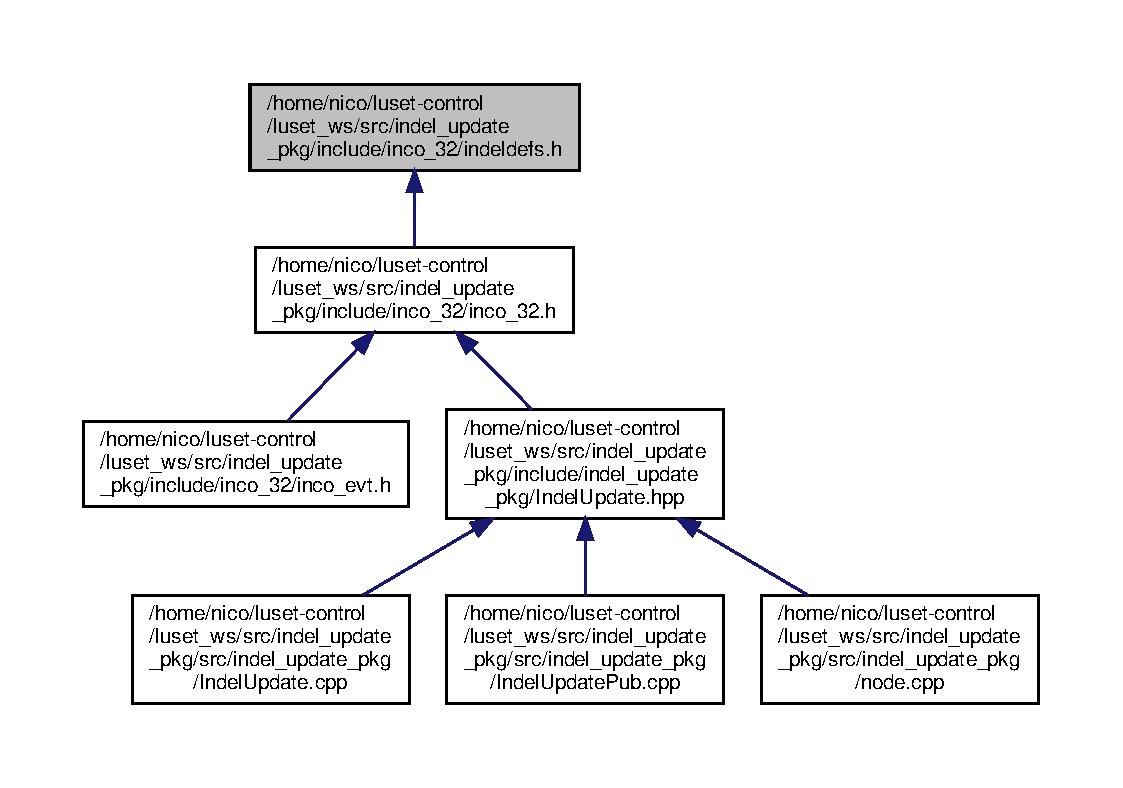
\includegraphics[width=350pt]{indeldefs_8h__dep__incl}
\end{center}
\end{figure}
\subsection*{Macros}
\begin{DoxyCompactItemize}
\item 
\#define \hyperlink{indeldefs_8h_a2e46908e658b77f17b25ad81bf988bd4}{D\+F\+\_\+\+I\+N\+C\+O\+\_\+\+A\+S\+Y\+N\+C\+\_\+\+R\+E\+S\+U\+L\+T\+\_\+\+S\+T\+R\+I\+N\+G\+\_\+\+M\+AX}~1024
\end{DoxyCompactItemize}
\begin{Indent}\textbf{ I\+N\+CO type target characteristics}\par
\begin{DoxyCompactItemize}
\item 
\#define \hyperlink{indeldefs_8h_a5e950b4cfa88414794985f4ac16906cb}{D\+F\+\_\+\+S\+L\+A\+V\+E\+\_\+\+C\+H\+A\+R\+\_\+\+F\+L\+O\+AT}~0x00000001L
\begin{DoxyCompactList}\small\item\em floating point available \end{DoxyCompactList}\end{DoxyCompactItemize}
\end{Indent}
\begin{Indent}\textbf{ I\+N\+CO type manipulation flags}\par
\begin{DoxyCompactItemize}
\item 
\#define \hyperlink{indeldefs_8h_ad53e1ca1e9ce83b47e7d043cfb8e8017}{D\+F\+\_\+\+I\+N\+C\+O\+\_\+\+T\+Y\+P\+E\+\_\+\+M\+A\+S\+K\+\_\+\+T\+Y\+P\+E\+\_\+\+O\+N\+LY}~0x0\+F\+FF
\begin{DoxyCompactList}\small\item\em Use this mask to get rid of any flags, such as the def\+Type\+\_\+\+With\+\_\+\+Name. \end{DoxyCompactList}\item 
\#define \hyperlink{indeldefs_8h_a102163e0ab1a744229dc5d62d31397d3}{D\+F\+\_\+\+I\+N\+C\+O\+\_\+\+T\+Y\+P\+E\+\_\+\+W\+I\+T\+H\+\_\+\+N\+A\+ME}~0x8000
\begin{DoxyCompactList}\small\item\em \char`\"{}flag\char`\"{} that indicates that the data is sent including its name. Used e.\+g. by the async callprocedure mechanism if results are named. \end{DoxyCompactList}\end{DoxyCompactItemize}
\end{Indent}
\begin{Indent}\textbf{ I\+N\+CO type definitions}\par
\begin{DoxyCompactItemize}
\item 
\#define \hyperlink{indeldefs_8h_a272b59f698fdb3dd19df76629970d1e7}{D\+F\+\_\+\+I\+N\+C\+O\+\_\+\+T\+Y\+P\+E\+\_\+\+I\+N\+V\+A\+L\+ID}~0x7\+F\+FF
\begin{DoxyCompactList}\small\item\em invalid or undefined I\+N\+CO type \end{DoxyCompactList}\item 
\#define \hyperlink{indeldefs_8h_ac21bea9bcbc9ac97ed67f4f6802d21fe}{D\+F\+\_\+\+I\+N\+C\+O\+\_\+\+T\+Y\+P\+E\+\_\+\+O\+B\+J\+E\+CT}~0x0000
\begin{DoxyCompactList}\small\item\em type object \end{DoxyCompactList}\item 
\#define \hyperlink{indeldefs_8h_ac09007dea7a37116d0dbb42fc793139a}{D\+F\+\_\+\+I\+N\+C\+O\+\_\+\+T\+Y\+P\+E\+\_\+\+S\+U\+B\+P\+L\+U\+G\+IN}~0x0001
\begin{DoxyCompactList}\small\item\em type I\+N\+C\+O-\/\+Sub\+Plugin \end{DoxyCompactList}\item 
\#define \hyperlink{indeldefs_8h_a56f80c6b43538f7d09cfc0ba6683f8e3}{D\+F\+\_\+\+I\+N\+C\+O\+\_\+\+T\+Y\+P\+E\+\_\+\+V\+A\+R\+I\+A\+B\+LE}~0x0100
\begin{DoxyCompactList}\small\item\em type variable \end{DoxyCompactList}\item 
\#define \hyperlink{indeldefs_8h_a6656d12e1a33c43e17f7389097f6e9fc}{D\+F\+\_\+\+I\+N\+C\+O\+\_\+\+T\+Y\+P\+E\+\_\+\+U\+I\+N\+T64}~0x0101
\begin{DoxyCompactList}\small\item\em type uint32 \end{DoxyCompactList}\item 
\#define \hyperlink{indeldefs_8h_a244b242e884fd70575b11c4926a21c66}{D\+F\+\_\+\+I\+N\+C\+O\+\_\+\+T\+Y\+P\+E\+\_\+\+I\+N\+T64}~0x0102
\begin{DoxyCompactList}\small\item\em type int32 \end{DoxyCompactList}\item 
\#define \hyperlink{indeldefs_8h_ab795ee7b5ee70f13bd4c1a0ae12bf163}{D\+F\+\_\+\+I\+N\+C\+O\+\_\+\+T\+Y\+P\+E\+\_\+\+U\+I\+N\+T32}~0x0103
\begin{DoxyCompactList}\small\item\em type uint32 \end{DoxyCompactList}\item 
\#define \hyperlink{indeldefs_8h_a2696bd1c35e91bac327b1fca402a2f02}{D\+F\+\_\+\+I\+N\+C\+O\+\_\+\+T\+Y\+P\+E\+\_\+\+I\+N\+T32}~0x0104
\begin{DoxyCompactList}\small\item\em type int32 \end{DoxyCompactList}\item 
\#define \hyperlink{indeldefs_8h_a273ba67bb59795b08e606c4dab125d77}{D\+F\+\_\+\+I\+N\+C\+O\+\_\+\+T\+Y\+P\+E\+\_\+\+U\+I\+N\+T16}~0x0105
\begin{DoxyCompactList}\small\item\em type uint16 \end{DoxyCompactList}\item 
\#define \hyperlink{indeldefs_8h_a88552c9a426a7707510de2ff99d067a9}{D\+F\+\_\+\+I\+N\+C\+O\+\_\+\+T\+Y\+P\+E\+\_\+\+I\+N\+T16}~0x0106
\begin{DoxyCompactList}\small\item\em type int16 \end{DoxyCompactList}\item 
\#define \hyperlink{indeldefs_8h_a67196d1983cb3ffd3eead24d2070402e}{D\+F\+\_\+\+I\+N\+C\+O\+\_\+\+T\+Y\+P\+E\+\_\+\+U\+I\+N\+T8}~0x0107
\begin{DoxyCompactList}\small\item\em type uint8 \end{DoxyCompactList}\item 
\#define \hyperlink{indeldefs_8h_a9734bdf1c35cb63919cf45a6a17c83c8}{D\+F\+\_\+\+I\+N\+C\+O\+\_\+\+T\+Y\+P\+E\+\_\+\+I\+N\+T8}~0x0108
\begin{DoxyCompactList}\small\item\em type int8 \end{DoxyCompactList}\item 
\#define \hyperlink{indeldefs_8h_a80eed31d4b0b9e1af9df2494f5f74f76}{D\+F\+\_\+\+I\+N\+C\+O\+\_\+\+T\+Y\+P\+E\+\_\+\+D\+O\+U\+B\+LE}~0x0109
\begin{DoxyCompactList}\small\item\em type double \end{DoxyCompactList}\item 
\#define \hyperlink{indeldefs_8h_a28b7d492470d310d41b8d5154a3a5837}{D\+F\+\_\+\+I\+N\+C\+O\+\_\+\+T\+Y\+P\+E\+\_\+\+F\+L\+O\+AT}~0x010A
\begin{DoxyCompactList}\small\item\em type float, single \end{DoxyCompactList}\item 
\#define \hyperlink{indeldefs_8h_a4a5300853246b7efeaebc4a73f06b207}{D\+F\+\_\+\+I\+N\+C\+O\+\_\+\+T\+Y\+P\+E\+\_\+\+D\+A\+T\+E\+T\+I\+ME}~0x010B
\begin{DoxyCompactList}\small\item\em type date/time \end{DoxyCompactList}\item 
\#define \hyperlink{indeldefs_8h_a5e8e5d93302d4b976d4634430d288230}{D\+F\+\_\+\+I\+N\+C\+O\+\_\+\+T\+Y\+P\+E\+\_\+\+B\+IT}~0x010C
\begin{DoxyCompactList}\small\item\em type bit \end{DoxyCompactList}\item 
\#define \hyperlink{indeldefs_8h_af813fb4f7d643bd59cf82a7d11fa5be6}{D\+F\+\_\+\+I\+N\+C\+O\+\_\+\+T\+Y\+P\+E\+\_\+\+F\+I\+X\+E\+D64}~0x010D
\begin{DoxyCompactList}\small\item\em type fixed64 \end{DoxyCompactList}\item 
\#define \hyperlink{indeldefs_8h_a00ae1be965ec5454d223d001dbb1e68e}{D\+F\+\_\+\+I\+N\+C\+O\+\_\+\+T\+Y\+P\+E\+\_\+\+F\+I\+X\+E\+D32}~0x010E
\begin{DoxyCompactList}\small\item\em type fixed32 \end{DoxyCompactList}\item 
\#define \hyperlink{indeldefs_8h_a3af18aa950836dfa670e58bbb72dbe43}{D\+F\+\_\+\+I\+N\+C\+O\+\_\+\+T\+Y\+P\+E\+\_\+\+D\+O\+U\+B\+L\+E\+\_\+\+N\+\_\+\+F\+I\+X\+E\+D64}~0x010F
\begin{DoxyCompactList}\small\item\em type double and fixed64 \end{DoxyCompactList}\item 
\#define \hyperlink{indeldefs_8h_a804807f8f50fe7983ad10c147976627d}{D\+F\+\_\+\+I\+N\+C\+O\+\_\+\+T\+Y\+P\+E\+\_\+\+F\+L\+O\+A\+T\+\_\+\+N\+\_\+\+F\+I\+X\+E\+D32}~0x0110
\begin{DoxyCompactList}\small\item\em type float and uint32 (used for very old style callprocedure (non-\/ex)). \end{DoxyCompactList}\item 
\#define \hyperlink{indeldefs_8h_ad040564795361355f35160e32ff0d631}{D\+F\+\_\+\+I\+N\+C\+O\+\_\+\+T\+Y\+P\+E\+\_\+\+B\+O\+O\+L\+E\+AN}~0x0111
\begin{DoxyCompactList}\small\item\em type bool using 8bit! (in constrast to D\+F\+\_\+\+I\+N\+C\+O\+\_\+\+T\+Y\+P\+E\+\_\+\+B\+O\+OL -\/ which is platform dependent) \end{DoxyCompactList}\item 
\#define \hyperlink{indeldefs_8h_a0f27c7a63f462a5f51c285c85d7a5cac}{D\+F\+\_\+\+I\+N\+C\+O\+\_\+\+T\+Y\+P\+E\+\_\+\+N\+U\+M\+B\+E\+R\+\_\+\+V\+A\+L\+UE}~0x0112
\begin{DoxyCompactList}\small\item\em type for \textquotesingle{}number values\textquotesingle{} that can be represented by a 64bit floating point number. (such as bool, (u)int8, 16, 32, float and double) \end{DoxyCompactList}\item 
\#define \hyperlink{indeldefs_8h_af4a276391f4493372bb023f924c836eb}{D\+F\+\_\+\+I\+N\+C\+O\+\_\+\+T\+Y\+P\+E\+\_\+\+P\+O\+I\+N\+T\+ER}~0x0113
\begin{DoxyCompactList}\small\item\em type I\+N\+CO (void$\ast$) pointer \end{DoxyCompactList}\item 
\#define \hyperlink{indeldefs_8h_abfef8fe4f879bf521466a2d4f722f4ff}{D\+F\+\_\+\+I\+N\+C\+O\+\_\+\+T\+Y\+P\+E\+\_\+\+S\+T\+R\+I\+NG}~0x0200
\begin{DoxyCompactList}\small\item\em type string \end{DoxyCompactList}\item 
\#define \hyperlink{indeldefs_8h_aa7e6de26ed5431fc292bc2b3b4b86100}{D\+F\+\_\+\+I\+N\+C\+O\+\_\+\+T\+Y\+P\+E\+\_\+\+F\+I\+LE}~0x0201
\begin{DoxyCompactList}\small\item\em type file (path/filename) \end{DoxyCompactList}\item 
\#define \hyperlink{indeldefs_8h_a0ffd16990beec1d4b34fb57bf305f85f}{D\+F\+\_\+\+I\+N\+C\+O\+\_\+\+T\+Y\+P\+E\+\_\+\+B\+I\+N\+A\+RY}~0x0202
\begin{DoxyCompactList}\small\item\em type binary (file data) \end{DoxyCompactList}\item 
\#define \hyperlink{indeldefs_8h_a0df9731611d0697e0f85d679c5aa7a7f}{D\+F\+\_\+\+I\+N\+C\+O\+\_\+\+T\+Y\+P\+E\+\_\+\+P\+R\+O\+C\+E\+D\+U\+RE}~0x0300
\begin{DoxyCompactList}\small\item\em type procedure \end{DoxyCompactList}\end{DoxyCompactItemize}
\end{Indent}
\begin{Indent}\textbf{ I\+N\+CO type flags. They can be passed to some functions, such as Call\+Procedure\+Ex\+Result}\par
\begin{DoxyCompactItemize}
\item 
\#define \hyperlink{indeldefs_8h_a2ced59a9816ac78eecb66761e6c56aa8}{D\+F\+\_\+\+I\+N\+C\+O\+\_\+\+F\+L\+A\+G\+\_\+\+G\+E\+T\+\_\+\+R\+E\+S\+U\+L\+T\+\_\+\+T\+Y\+PE}~0x00010000L
\begin{DoxyCompactList}\small\item\em flag to get the type of the result value. result type is expected to be uint32 \end{DoxyCompactList}\item 
\#define \hyperlink{indeldefs_8h_a38b4f4618d6964e94b19df39dc340af5}{D\+F\+\_\+\+I\+N\+C\+O\+\_\+\+F\+L\+A\+G\+\_\+\+G\+E\+T\+\_\+\+R\+E\+S\+U\+L\+T\+\_\+\+L\+E\+N\+G\+TH}~0x00020000L
\begin{DoxyCompactList}\small\item\em flag to get the length of the result value. result type is expected to be uint32 \end{DoxyCompactList}\end{DoxyCompactItemize}
\end{Indent}
\begin{Indent}\textbf{ I\+N\+CO item characteristics}\par
\begin{DoxyCompactItemize}
\item 
\#define \hyperlink{indeldefs_8h_ae94758ba78adfc51f0c9334464e9551a}{D\+F\+\_\+\+I\+N\+C\+O\+\_\+\+C\+H\+A\+R\+\_\+\+R\+E\+A\+D\+\_\+\+O\+N\+LY}~0x00000001L
\begin{DoxyCompactList}\small\item\em variable is read only \end{DoxyCompactList}\item 
\#define \hyperlink{indeldefs_8h_aaaa0f14d4d4cb6991088944e81447416}{D\+F\+\_\+\+I\+N\+C\+O\+\_\+\+C\+H\+A\+R\+\_\+\+I\+N\+V\+I\+S\+I\+B\+LE}~0x00000002L
\begin{DoxyCompactList}\small\item\em variable is invisible \end{DoxyCompactList}\item 
\#define \hyperlink{indeldefs_8h_aa6955ec6298c0981af7f2c52a384161d}{D\+F\+\_\+\+I\+N\+C\+O\+\_\+\+C\+H\+A\+R\+\_\+\+O\+B\+J\+E\+C\+T\+\_\+\+W\+I\+T\+H\+\_\+\+V\+A\+L\+UE}~0x00000004L
\begin{DoxyCompactList}\small\item\em object has value (member with same name) \end{DoxyCompactList}\item 
\#define \hyperlink{indeldefs_8h_a6622a67d8b79180c47aaf7b02afc76df}{D\+F\+\_\+\+I\+N\+C\+O\+\_\+\+C\+H\+A\+R\+\_\+\+O\+B\+J\+E\+C\+T\+\_\+\+N\+O\+\_\+\+M\+E\+M\+B\+ER}~0x00000008L
\begin{DoxyCompactList}\small\item\em object has no members \end{DoxyCompactList}\item 
\#define \hyperlink{indeldefs_8h_ad682d5018a992246f4d3ac2f83ddc333}{D\+F\+\_\+\+I\+N\+C\+O\+\_\+\+C\+H\+A\+R\+\_\+\+M\+U\+S\+T\+\_\+\+C\+A\+LL}~0x00004000L
\begin{DoxyCompactList}\small\item\em should be called with Get() \end{DoxyCompactList}\item 
\#define \hyperlink{indeldefs_8h_abd117318d1ff63790a3a8702f7469f48}{D\+F\+\_\+\+I\+N\+C\+O\+\_\+\+C\+H\+A\+R\+\_\+\+S\+H\+O\+W\+\_\+\+E\+XP}~0x00000000L
\begin{DoxyCompactList}\small\item\em show item in exponential \end{DoxyCompactList}\item 
\#define \hyperlink{indeldefs_8h_a342f337fa3dbc60464604fb375fdc748}{D\+F\+\_\+\+I\+N\+C\+O\+\_\+\+C\+H\+A\+R\+\_\+\+S\+H\+O\+W\+\_\+\+H\+EX}~0x00000004L
\begin{DoxyCompactList}\small\item\em show item in hexadecimal \end{DoxyCompactList}\item 
\#define \hyperlink{indeldefs_8h_a1d865c7b127512a9b37e70ea39a10536}{D\+F\+\_\+\+I\+N\+C\+O\+\_\+\+C\+H\+A\+R\+\_\+\+S\+H\+O\+W\+\_\+\+D\+EC}~0x00000008L
\begin{DoxyCompactList}\small\item\em show item in decimal \end{DoxyCompactList}\item 
\#define \hyperlink{indeldefs_8h_a25250cfb6cf784e0bf062427e08d0c83}{D\+F\+\_\+\+I\+N\+C\+O\+\_\+\+C\+H\+A\+R\+\_\+\+O\+B\+J\+E\+C\+T\+\_\+\+B\+MP}~0x00000010L
\begin{DoxyCompactList}\small\item\em take bitmap from parent folder \end{DoxyCompactList}\item 
\#define \hyperlink{indeldefs_8h_a92e746c0c40f8e4e4bd3bfe0d69f18d3}{D\+F\+\_\+\+I\+N\+C\+O\+\_\+\+C\+H\+A\+R\+\_\+\+S\+H\+O\+W\+\_\+\+F\+IX}~0x0000000\+CL
\begin{DoxyCompactList}\small\item\em show item in fixed point \end{DoxyCompactList}\item 
\#define \hyperlink{indeldefs_8h_a9dc97ba4e6eb122410d367d86e328ff4}{D\+F\+\_\+\+I\+N\+C\+O\+\_\+\+C\+H\+A\+R\+\_\+\+S\+H\+O\+W\+\_\+\+D\+I\+G\+\_\+1}~0x00000010L
\begin{DoxyCompactList}\small\item\em show 1 digit after point \end{DoxyCompactList}\item 
\#define \hyperlink{indeldefs_8h_a3881ea739c3b19b420d8a9a4b79cb56b}{D\+F\+\_\+\+I\+N\+C\+O\+\_\+\+C\+H\+A\+R\+\_\+\+S\+H\+O\+W\+\_\+\+D\+I\+G\+\_\+2}~0x00000020L
\begin{DoxyCompactList}\small\item\em show 2 digit after point \end{DoxyCompactList}\item 
\#define \hyperlink{indeldefs_8h_ad4ba7783a022c3b7fce97e9822ea54af}{D\+F\+\_\+\+I\+N\+C\+O\+\_\+\+C\+H\+A\+R\+\_\+\+S\+H\+O\+W\+\_\+\+D\+I\+G\+\_\+3}~0x00000030L
\begin{DoxyCompactList}\small\item\em show 3 digit after point \end{DoxyCompactList}\item 
\#define \hyperlink{indeldefs_8h_ac2b27fec4b8c9deb0521a83f52680955}{D\+F\+\_\+\+I\+N\+C\+O\+\_\+\+C\+H\+A\+R\+\_\+\+S\+H\+O\+W\+\_\+\+D\+I\+G\+\_\+4}~0x00000040L
\begin{DoxyCompactList}\small\item\em show 4 digit after point \end{DoxyCompactList}\item 
\#define \hyperlink{indeldefs_8h_a5946a93809c2d7d928e606a17a6d3a86}{D\+F\+\_\+\+I\+N\+C\+O\+\_\+\+C\+H\+A\+R\+\_\+\+S\+H\+O\+W\+\_\+\+D\+I\+G\+\_\+5}~0x00000050L
\begin{DoxyCompactList}\small\item\em show 5 digit after point \end{DoxyCompactList}\item 
\#define \hyperlink{indeldefs_8h_a5b15b9490130a2153f86bf3fc75a5e95}{D\+F\+\_\+\+I\+N\+C\+O\+\_\+\+C\+H\+A\+R\+\_\+\+S\+H\+O\+W\+\_\+\+D\+I\+G\+\_\+6}~0x00000060L
\begin{DoxyCompactList}\small\item\em show 6 digit after point \end{DoxyCompactList}\item 
\#define \hyperlink{indeldefs_8h_a8ff43b724b622b3249872e17d64ab220}{D\+F\+\_\+\+I\+N\+C\+O\+\_\+\+C\+H\+A\+R\+\_\+\+S\+H\+O\+W\+\_\+\+D\+I\+G\+\_\+7}~0x00000070L
\begin{DoxyCompactList}\small\item\em show 7 digit after point \end{DoxyCompactList}\item 
\#define \hyperlink{indeldefs_8h_aaa682a67946795c8913ed4161c723c15}{D\+F\+\_\+\+I\+N\+C\+O\+\_\+\+C\+H\+A\+R\+\_\+\+S\+H\+O\+W\+\_\+\+D\+I\+G\+\_\+8}~0x00000080L
\begin{DoxyCompactList}\small\item\em show 8 digit after point \end{DoxyCompactList}\item 
\#define \hyperlink{indeldefs_8h_a644574723531f076807afadaa65464a0}{D\+F\+\_\+\+I\+N\+C\+O\+\_\+\+C\+H\+A\+R\+\_\+\+S\+H\+O\+W\+\_\+\+D\+I\+G\+\_\+9}~0x00000090L
\begin{DoxyCompactList}\small\item\em show 9 digit after point \end{DoxyCompactList}\item 
\#define \hyperlink{indeldefs_8h_a2c75903b3319c15c4f5881c56dd9ccb4}{D\+F\+\_\+\+I\+N\+C\+O\+\_\+\+C\+H\+A\+R\+\_\+\+S\+H\+O\+W\+\_\+\+D\+I\+G\+\_\+10}~0x000000\+A0L
\begin{DoxyCompactList}\small\item\em show 10 digit after point \end{DoxyCompactList}\item 
\#define \hyperlink{indeldefs_8h_ae11336f7445356bf28fe8a961de2a201}{D\+F\+\_\+\+I\+N\+C\+O\+\_\+\+C\+H\+A\+R\+\_\+\+S\+H\+O\+W\+\_\+\+D\+I\+G\+\_\+11}~0x000000\+B0L
\begin{DoxyCompactList}\small\item\em show 11 digit after point \end{DoxyCompactList}\item 
\#define \hyperlink{indeldefs_8h_aae9222179c54a52eaf198e0a5183c39e}{D\+F\+\_\+\+I\+N\+C\+O\+\_\+\+C\+H\+A\+R\+\_\+\+S\+H\+O\+W\+\_\+\+D\+I\+G\+\_\+12}~0x000000\+C0L
\begin{DoxyCompactList}\small\item\em show 12 digit after point \end{DoxyCompactList}\item 
\#define \hyperlink{indeldefs_8h_a01e7a7f8c52d49d4762787e724cbb112}{D\+F\+\_\+\+I\+N\+C\+O\+\_\+\+C\+H\+A\+R\+\_\+\+S\+H\+O\+W\+\_\+\+D\+I\+G\+\_\+13}~0x000000\+D0L
\begin{DoxyCompactList}\small\item\em show 13 digit after point \end{DoxyCompactList}\item 
\#define \hyperlink{indeldefs_8h_ae0de38f1a20e3e2c1eb9da7b3a84882a}{D\+F\+\_\+\+I\+N\+C\+O\+\_\+\+C\+H\+A\+R\+\_\+\+S\+H\+O\+W\+\_\+\+D\+I\+G\+\_\+14}~0x000000\+E0L
\begin{DoxyCompactList}\small\item\em show 14 digit after point \end{DoxyCompactList}\item 
\#define \hyperlink{indeldefs_8h_a957e4e0bb12c095e029e359ea663d63e}{D\+F\+\_\+\+I\+N\+C\+O\+\_\+\+C\+H\+A\+R\+\_\+\+S\+H\+O\+W\+\_\+\+D\+I\+G\+\_\+15}~0x000000\+F0L
\begin{DoxyCompactList}\small\item\em show 15 digit after point \end{DoxyCompactList}\item 
\#define \hyperlink{indeldefs_8h_a5c7f260698e06a80c49e5e1c1311f6c3}{D\+F\+\_\+\+I\+N\+C\+O\+\_\+\+C\+H\+A\+R\+\_\+\+S\+H\+O\+W\+\_\+\+E\+N\+G\+\_\+0}~0x00000018L
\begin{DoxyCompactList}\small\item\em show item in engineering notation with 0 decimal places \end{DoxyCompactList}\item 
\#define \hyperlink{indeldefs_8h_aac9590b1d806416bcf7ca01aa5abec03}{D\+F\+\_\+\+I\+N\+C\+O\+\_\+\+C\+H\+A\+R\+\_\+\+S\+H\+O\+W\+\_\+\+E\+N\+G\+\_\+1}~0x00000028L
\begin{DoxyCompactList}\small\item\em show item in engineering notation with 1 decimal place \end{DoxyCompactList}\item 
\#define \hyperlink{indeldefs_8h_a2cbd7d57e629c79bf3e73f8c9baaae27}{D\+F\+\_\+\+I\+N\+C\+O\+\_\+\+C\+H\+A\+R\+\_\+\+S\+H\+O\+W\+\_\+\+E\+N\+G\+\_\+2}~0x00000038L
\begin{DoxyCompactList}\small\item\em show item in engineering notation with 2 decimal places \end{DoxyCompactList}\item 
\#define \hyperlink{indeldefs_8h_ad6c0cf1547a80f66004194aaa43c9b7a}{D\+F\+\_\+\+I\+N\+C\+O\+\_\+\+C\+H\+A\+R\+\_\+\+S\+H\+O\+W\+\_\+\+E\+N\+G\+\_\+3}~0x00000048L
\begin{DoxyCompactList}\small\item\em show item in engineering notation with 3 decimal places \end{DoxyCompactList}\item 
\#define \hyperlink{indeldefs_8h_aa6ff326570dc251f57cc3dad25e576bf}{D\+F\+\_\+\+I\+N\+C\+O\+\_\+\+C\+H\+A\+R\+\_\+\+S\+H\+O\+W\+\_\+\+E\+N\+G\+\_\+4}~0x00000058L
\begin{DoxyCompactList}\small\item\em show item in engineering notation with 4 decimal places \end{DoxyCompactList}\item 
\#define \hyperlink{indeldefs_8h_a57b9675957c47620bff146ac2dfe1f26}{D\+F\+\_\+\+I\+N\+C\+O\+\_\+\+C\+H\+A\+R\+\_\+\+S\+H\+O\+W\+\_\+\+E\+N\+G\+\_\+5}~0x00000068L
\begin{DoxyCompactList}\small\item\em show item in engineering notation with 5 decimal places \end{DoxyCompactList}\item 
\#define \hyperlink{indeldefs_8h_a2b9fb21f1c4a68880a5c0907aaf3fc53}{D\+F\+\_\+\+I\+N\+C\+O\+\_\+\+C\+H\+A\+R\+\_\+\+S\+H\+O\+W\+\_\+\+E\+N\+G\+\_\+6}~0x00000078L
\begin{DoxyCompactList}\small\item\em show item in engineering notation with 6 decimal places \end{DoxyCompactList}\item 
\#define \hyperlink{indeldefs_8h_a6b7306f63aeef7428508b540c7bb876a}{D\+F\+\_\+\+I\+N\+C\+O\+\_\+\+C\+H\+A\+R\+\_\+\+S\+H\+O\+W\+\_\+\+E\+N\+G\+\_\+7}~0x00000088L
\begin{DoxyCompactList}\small\item\em show item in engineering notation with 7 decimal places \end{DoxyCompactList}\item 
\#define \hyperlink{indeldefs_8h_aed561b6167345b6ca736ab55e78bcb4d}{D\+F\+\_\+\+I\+N\+C\+O\+\_\+\+C\+H\+A\+R\+\_\+\+S\+H\+O\+W\+\_\+\+E\+N\+G\+\_\+8}~0x00000098L
\begin{DoxyCompactList}\small\item\em show item in engineering notation with 8 decimal places \end{DoxyCompactList}\item 
\#define \hyperlink{indeldefs_8h_a37b093c59378bcf8aa21de785c882de5}{D\+F\+\_\+\+I\+N\+C\+O\+\_\+\+C\+H\+A\+R\+\_\+\+S\+H\+O\+W\+\_\+\+E\+N\+G\+\_\+9}~0x000000\+A8L
\begin{DoxyCompactList}\small\item\em show item in engineering notation with 9 decimal places \end{DoxyCompactList}\item 
\#define \hyperlink{indeldefs_8h_a159976722b42a7aac66653192f11371d}{D\+F\+\_\+\+I\+N\+C\+O\+\_\+\+C\+H\+A\+R\+\_\+\+S\+H\+O\+W\+\_\+\+E\+N\+G\+\_\+10}~0x000000\+B8L
\begin{DoxyCompactList}\small\item\em show item in engineering notation with 10 decimal places \end{DoxyCompactList}\item 
\#define \hyperlink{indeldefs_8h_abadbb86cbd2d62ea176ed8d05653ce12}{D\+F\+\_\+\+I\+N\+C\+O\+\_\+\+C\+H\+A\+R\+\_\+\+S\+H\+O\+W\+\_\+\+E\+N\+G\+\_\+11}~0x000000\+C8L
\begin{DoxyCompactList}\small\item\em show item in engineering notation with 11 decimal places \end{DoxyCompactList}\item 
\#define \hyperlink{indeldefs_8h_a9f5d3f9ca4a551d33ee4ab74181c17a1}{D\+F\+\_\+\+I\+N\+C\+O\+\_\+\+C\+H\+A\+R\+\_\+\+S\+H\+O\+W\+\_\+\+E\+N\+G\+\_\+12}~0x000000\+D8L
\begin{DoxyCompactList}\small\item\em show item in engineering notation with 12 decimal places \end{DoxyCompactList}\item 
\#define \hyperlink{indeldefs_8h_a90ee175d9247265d7dc6bb56e63a04bc}{D\+F\+\_\+\+I\+N\+C\+O\+\_\+\+C\+H\+A\+R\+\_\+\+S\+H\+O\+W\+\_\+\+E\+N\+G\+\_\+13}~0x000000\+E8L
\begin{DoxyCompactList}\small\item\em show item in engineering notation with 13 decimal places \end{DoxyCompactList}\item 
\#define \hyperlink{indeldefs_8h_a134af70a29dbee057cd2014b9d19c020}{D\+F\+\_\+\+I\+N\+C\+O\+\_\+\+C\+H\+A\+R\+\_\+\+S\+H\+O\+W\+\_\+\+E\+N\+G\+\_\+14}~0x000000\+F8L
\begin{DoxyCompactList}\small\item\em show item in engineering notation with 14 decimal places \end{DoxyCompactList}\item 
\#define \hyperlink{indeldefs_8h_ab5e821114473ed38acc17e28fb600b2b}{D\+F\+\_\+\+I\+N\+C\+O\+\_\+\+C\+H\+A\+R\+\_\+\+B\+M\+P\+\_\+\+ID}~0x00\+F\+F0000L
\begin{DoxyCompactList}\small\item\em bitmap id (1..223 for user, 224..255 for predefined bitmaps) \end{DoxyCompactList}\item 
\#define \hyperlink{indeldefs_8h_a2b222dbe41643c7ee0e4043555d826ba}{D\+F\+\_\+\+I\+N\+C\+O\+\_\+\+C\+H\+A\+R\+\_\+\+H\+A\+S\+C\+O\+M\+B\+O\+B\+OX}~0x01000000L
\begin{DoxyCompactList}\small\item\em item has a combobox \end{DoxyCompactList}\item 
\#define \hyperlink{indeldefs_8h_a21c9cd09fe9456c86d26cefecb06e061}{D\+F\+\_\+\+I\+N\+C\+O\+\_\+\+C\+H\+A\+R\+\_\+\+M\+U\+S\+T\+D\+E\+L\+E\+TE}~0x02000000L
\begin{DoxyCompactList}\small\item\em item has to be deleted in inco-\/exp if not found \end{DoxyCompactList}\item 
\#define \hyperlink{indeldefs_8h_a07b22c2d8add79da7f2db354483cd913}{D\+F\+\_\+\+I\+N\+C\+O\+\_\+\+C\+H\+A\+R\+\_\+\+I\+N\+T\+E\+R\+N\+A\+L\+U\+SE}~0x04000000L
\begin{DoxyCompactList}\small\item\em more invisible than def\+Char\+Invisible \end{DoxyCompactList}\item 
\#define \hyperlink{indeldefs_8h_ac32f5aacdb1d4a05f78624d614c8bd95}{D\+F\+\_\+\+I\+N\+C\+O\+\_\+\+C\+H\+A\+R\+\_\+\+H\+A\+S\+E\+X\+T\+C\+O\+N\+F\+IG}~0x08000000l
\begin{DoxyCompactList}\small\item\em item has extended config (characteristics2) \end{DoxyCompactList}\item 
\#define \hyperlink{indeldefs_8h_abef171db8762687209fa959faf6ef045}{D\+F\+\_\+\+I\+N\+C\+O\+\_\+\+C\+H\+A\+R\+\_\+\+T\+O\+U\+C\+H\+ED}~0x80000000L
\begin{DoxyCompactList}\small\item\em item touched \end{DoxyCompactList}\end{DoxyCompactItemize}
\end{Indent}
\begin{Indent}\textbf{ I\+N\+CO item extended characeristics}\par
\begin{DoxyCompactItemize}
\item 
\#define \hyperlink{indeldefs_8h_acc8392ad43df69a16061ae53699f5613}{D\+F\+\_\+\+I\+N\+C\+O\+\_\+\+C\+H\+A\+R2\+\_\+\+C\+O\+L\+O\+RS}~0x00000001l
\begin{DoxyCompactList}\small\item\em item has fore-\/ and backcolor \end{DoxyCompactList}\item 
\#define \hyperlink{indeldefs_8h_a7cf1e1ce6831486c313fa889783a70f9}{D\+F\+\_\+\+I\+N\+C\+O\+\_\+\+C\+H\+A\+R2\+\_\+\+P\+E\+R\+S\+I\+S\+T\+E\+NT}~0x00000002l
\begin{DoxyCompactList}\small\item\em item value is saved in I\+GD file (I\+N\+IX) \end{DoxyCompactList}\item 
\#define \hyperlink{indeldefs_8h_ac360214873439c04232fc572978e3e8e}{D\+F\+\_\+\+I\+N\+C\+O\+\_\+\+C\+H\+A\+R2\+\_\+\+T\+R\+I\+G\+G\+E\+R\+\_\+\+S\+U\+PP}~0x00000004l
\begin{DoxyCompactList}\small\item\em item supports triggers (I\+N\+IX) \end{DoxyCompactList}\item 
\#define \hyperlink{indeldefs_8h_a722a8c2d1145c82adad7275c91d37bd1}{D\+F\+\_\+\+I\+N\+C\+O\+\_\+\+C\+H\+A\+R2\+\_\+\+A\+L\+I\+G\+N\+\_\+\+R\+I\+G\+HT}~0x00000008l
\begin{DoxyCompactList}\small\item\em display value right-\/aligned \end{DoxyCompactList}\item 
\#define \hyperlink{indeldefs_8h_a9a423959591830e6b394f97e72885f97}{D\+F\+\_\+\+I\+N\+C\+O\+\_\+\+C\+H\+A\+R2\+\_\+\+A\+L\+I\+G\+N\+\_\+\+L\+E\+FT}~0x00000010l
\begin{DoxyCompactList}\small\item\em display value left-\/aligned \end{DoxyCompactList}\item 
\#define \hyperlink{indeldefs_8h_ad0656742f36a7d86cffcaa6409507375}{D\+F\+\_\+\+I\+N\+C\+O\+\_\+\+C\+H\+A\+R2\+\_\+\+A\+L\+I\+G\+N\+\_\+\+C\+E\+N\+T\+ER}~0x00000018l
\begin{DoxyCompactList}\small\item\em display value centered \end{DoxyCompactList}\item 
\#define \hyperlink{indeldefs_8h_a64319afa457c9af3cc327677acc226bf}{D\+F\+\_\+\+I\+N\+C\+O\+\_\+\+C\+H\+A\+R2\+\_\+\+A\+L\+I\+G\+N\+\_\+\+M\+A\+SK}~0x00000018l
\begin{DoxyCompactList}\small\item\em all alignment flags \end{DoxyCompactList}\item 
\#define \hyperlink{indeldefs_8h_af04b060b821381b115647c1e251517f9}{D\+F\+\_\+\+I\+N\+C\+O\+\_\+\+C\+H\+A\+R2\+\_\+\+A\+S\+Y\+N\+C\+\_\+\+R\+E\+S\+U\+LT}~0x00000020l
\begin{DoxyCompactList}\small\item\em async result (e.\+g. async Call\+Procedure or Get\+Variable) \end{DoxyCompactList}\item 
\#define \hyperlink{indeldefs_8h_a714db1fd03436140daad047d48b822f8}{D\+F\+\_\+\+I\+N\+C\+O\+\_\+\+C\+H\+A\+R2\+\_\+\+R\+E\+T\+\_\+\+M\+C\+R\+E\+S\+U\+LT}~0x00000040l
\begin{DoxyCompactList}\small\item\em Call\+Procedure returns C\+Mc\+Result. \end{DoxyCompactList}\item 
\#define \hyperlink{indeldefs_8h_ae8c4dc2ccce24f81c077d788e21c247b}{D\+F\+\_\+\+I\+N\+C\+O\+\_\+\+C\+H\+A\+R2\+\_\+\+O\+V\+E\+R\+S\+A\+M\+P\+L\+ED}~0x00000080l
\begin{DoxyCompactList}\small\item\em variable is oversampled \end{DoxyCompactList}\end{DoxyCompactItemize}
\end{Indent}


\subsection{Detailed Description}
Various defines related to I\+N\+CO data types and item characteristics. 

\begin{DoxyAuthor}{Author}
Raphael Zulliger, \copyright{} I\+N\+D\+EL AG 
\end{DoxyAuthor}
\begin{DoxyVersion}{Version}
1.\+00 \begin{DoxyVerb}1.00    03.02.2005-RZ : + origin

876, 2006-08-23 08:28:09 +0200 (Mi, 23 Aug 2006), walther
+ Added DF_INCO_TYPE_INVALID (for CINCOValue, but may also be useful elsewhere).

895, 2006-08-25 11:37:13 +0200 (Fri, 25 Aug 2006), walther
+ Merged changes from branches/simplification r851:891 to trunk.

1657, 2007-06-27 10:47:34 +0200 (Mi, 27 Jun 2007), walther
! Cleaning up the mess caused by committing r1656 even with icommit.py... :|

2222, 2007-11-29 17:03:48 +0100 (Do, 29 Nov 2007), zulliger


2295, 2007-12-14 18:04:05 +0100 (Fr, 14 Dez 2007), zulliger
! Many many changes. Too much to list in detail. But: A lot of McINCOFrame
  adjustments (especially regarding little/big-endian), a lot of cleanups
  in library structure, etc.

2322, 2007-12-18 09:15:36 +0100 (Di, 18 Dez 2007), zulliger
! Renamed indellib to libindel to have consistent naming. Change all
  includes in all projects to #include <indel/whatever.h>. Note: currently,
  ibuild.py will still create the ${INDEL_ROOT}/include/indellib folder for
  backward compatibility

2323, 2007-12-18 10:49:05 +0100 (Di, 18 Dez 2007), zulliger
! Changes needed because some headers were moved to the new 'inco_32'
  include folder

2347, 2007-12-18 11:46:17 +0100 (Di, 18 Dez 2007), zulliger
+ Added missing defintions

2357, 2007-12-18 17:15:35 +0100 (Di, 18 Dez 2007), walther
+ Introduced the ENG number format for engineering notation (multiple-of-3
  exponents). The constant coincides with DEC, ENG notation is used if the
  number of decimal places specified in the characteristics is greater than
  zero (due to this, the actual number of decimal places displayed is one
  less than what the characteristics field says).

2360, 2007-12-19 07:46:05 +0100 (Mi, 19 Dez 2007), walther
+ Added characteristics constant for the "touched" bit.

2382, 2007-12-20 16:06:51 +0100 (Do, 20 Dez 2007), zulliger
- Removed obsolete INCO type: list. It was used for inco path extensions
  like '*', '?', etc.

2384, 2007-12-20 18:08:09 +0100 (Do, 20 Dez 2007), zulliger
! Fixed bug: float arguments of callprocedures sent to non-float targets
  were wrongly converted. They are were sent as fixed32, but INOS expects
  them to be uint32

2421, 2008-01-04 07:08:08 +0100 (Fr, 04 Jan 2008), zulliger
+ Added some definitions used by IncoExp.
- Removed defs which are already defined by inco_32.h

3202, 2008-09-16 14:00:16 +0200 (Di, 16 Sep 2008), walther
+ I knew there was another place where characteristics constants were
  kept... adding the new ones from inos r1306 / libinix r3190.

-1,,
+ Added Inco alignment mask.

4185, 2010-06-10 16:33:52 +0200 (Do, 10 Jun 2010), zulliger
+ New INCO type and flag definitions required for async callprocedure 
  handling.

4211, 2010-06-15 15:55:54 +0200 (Di, 15 Jun 2010), zulliger
! Doxygenized documentation

4213, 2010-06-15 16:03:29 +0200 (Di, 15 Jun 2010), walther
+ Added DF_INCO_FLAG_GET_RESULT_LENGTH.

4229, 2010-06-16 16:58:36 +0200 (Mi, 16 Jun 2010), walther
! Documentation tweaks.

4234, 2010-06-17 14:34:51 +0200 (Thu, 17 Jun 2010), zulliger
! Synchronized types with INOS by adding DF_INCO_TYPE_POINTER

4726, 2010-12-31 11:35:07 +0100 (Fr, 31 Dez 2010), tjericke
+ Added some comments to the INCO type declarations, to keep all INCO
  declerations consistent.

4731, 2011-01-04 14:13:45 +0100 (Di, 04 Jan 2011), tjericke
+ Re-added accidentally deleted lines.

5099, 2012-01-19 18:06:20 +0100 (Don, 19 Jan 2012), hirzel
+ Added DF_INCO_CHAR2_OVERSAMPLED.

$LastChangedRevision: 6734 $ $Date: 2017-02-20 17:31:23 +0100 (Mon, 20 Feb 2017) $ $Author: zulliger $
+ Added 'DF_INCO_ASYNC_RESULT_STRING_MAX' which defines the maximum payload
  of an async callprocedure result.

$Comment$

u = unreleased
+ = new feature
! = change, bugfix
- = removed\end{DoxyVerb}

\end{DoxyVersion}
\begin{DoxyRemark}{Remarks}
\begin{DoxyVerb}project         : IndelLib
language        : C++ (Gnu, Visual C++)
system          : Linux, Windows
\end{DoxyVerb}
 
\end{DoxyRemark}


\subsection{Macro Definition Documentation}
\mbox{\Hypertarget{indeldefs_8h_a2e46908e658b77f17b25ad81bf988bd4}\label{indeldefs_8h_a2e46908e658b77f17b25ad81bf988bd4}} 
\index{indeldefs.\+h@{indeldefs.\+h}!D\+F\+\_\+\+I\+N\+C\+O\+\_\+\+A\+S\+Y\+N\+C\+\_\+\+R\+E\+S\+U\+L\+T\+\_\+\+S\+T\+R\+I\+N\+G\+\_\+\+M\+AX@{D\+F\+\_\+\+I\+N\+C\+O\+\_\+\+A\+S\+Y\+N\+C\+\_\+\+R\+E\+S\+U\+L\+T\+\_\+\+S\+T\+R\+I\+N\+G\+\_\+\+M\+AX}}
\index{D\+F\+\_\+\+I\+N\+C\+O\+\_\+\+A\+S\+Y\+N\+C\+\_\+\+R\+E\+S\+U\+L\+T\+\_\+\+S\+T\+R\+I\+N\+G\+\_\+\+M\+AX@{D\+F\+\_\+\+I\+N\+C\+O\+\_\+\+A\+S\+Y\+N\+C\+\_\+\+R\+E\+S\+U\+L\+T\+\_\+\+S\+T\+R\+I\+N\+G\+\_\+\+M\+AX}!indeldefs.\+h@{indeldefs.\+h}}
\subsubsection{\texorpdfstring{D\+F\+\_\+\+I\+N\+C\+O\+\_\+\+A\+S\+Y\+N\+C\+\_\+\+R\+E\+S\+U\+L\+T\+\_\+\+S\+T\+R\+I\+N\+G\+\_\+\+M\+AX}{DF\_INCO\_ASYNC\_RESULT\_STRING\_MAX}}
{\footnotesize\ttfamily \#define D\+F\+\_\+\+I\+N\+C\+O\+\_\+\+A\+S\+Y\+N\+C\+\_\+\+R\+E\+S\+U\+L\+T\+\_\+\+S\+T\+R\+I\+N\+G\+\_\+\+M\+AX~1024}

\mbox{\Hypertarget{indeldefs_8h_ad0656742f36a7d86cffcaa6409507375}\label{indeldefs_8h_ad0656742f36a7d86cffcaa6409507375}} 
\index{indeldefs.\+h@{indeldefs.\+h}!D\+F\+\_\+\+I\+N\+C\+O\+\_\+\+C\+H\+A\+R2\+\_\+\+A\+L\+I\+G\+N\+\_\+\+C\+E\+N\+T\+ER@{D\+F\+\_\+\+I\+N\+C\+O\+\_\+\+C\+H\+A\+R2\+\_\+\+A\+L\+I\+G\+N\+\_\+\+C\+E\+N\+T\+ER}}
\index{D\+F\+\_\+\+I\+N\+C\+O\+\_\+\+C\+H\+A\+R2\+\_\+\+A\+L\+I\+G\+N\+\_\+\+C\+E\+N\+T\+ER@{D\+F\+\_\+\+I\+N\+C\+O\+\_\+\+C\+H\+A\+R2\+\_\+\+A\+L\+I\+G\+N\+\_\+\+C\+E\+N\+T\+ER}!indeldefs.\+h@{indeldefs.\+h}}
\subsubsection{\texorpdfstring{D\+F\+\_\+\+I\+N\+C\+O\+\_\+\+C\+H\+A\+R2\+\_\+\+A\+L\+I\+G\+N\+\_\+\+C\+E\+N\+T\+ER}{DF\_INCO\_CHAR2\_ALIGN\_CENTER}}
{\footnotesize\ttfamily \#define D\+F\+\_\+\+I\+N\+C\+O\+\_\+\+C\+H\+A\+R2\+\_\+\+A\+L\+I\+G\+N\+\_\+\+C\+E\+N\+T\+ER~0x00000018l}



display value centered 

\mbox{\Hypertarget{indeldefs_8h_a9a423959591830e6b394f97e72885f97}\label{indeldefs_8h_a9a423959591830e6b394f97e72885f97}} 
\index{indeldefs.\+h@{indeldefs.\+h}!D\+F\+\_\+\+I\+N\+C\+O\+\_\+\+C\+H\+A\+R2\+\_\+\+A\+L\+I\+G\+N\+\_\+\+L\+E\+FT@{D\+F\+\_\+\+I\+N\+C\+O\+\_\+\+C\+H\+A\+R2\+\_\+\+A\+L\+I\+G\+N\+\_\+\+L\+E\+FT}}
\index{D\+F\+\_\+\+I\+N\+C\+O\+\_\+\+C\+H\+A\+R2\+\_\+\+A\+L\+I\+G\+N\+\_\+\+L\+E\+FT@{D\+F\+\_\+\+I\+N\+C\+O\+\_\+\+C\+H\+A\+R2\+\_\+\+A\+L\+I\+G\+N\+\_\+\+L\+E\+FT}!indeldefs.\+h@{indeldefs.\+h}}
\subsubsection{\texorpdfstring{D\+F\+\_\+\+I\+N\+C\+O\+\_\+\+C\+H\+A\+R2\+\_\+\+A\+L\+I\+G\+N\+\_\+\+L\+E\+FT}{DF\_INCO\_CHAR2\_ALIGN\_LEFT}}
{\footnotesize\ttfamily \#define D\+F\+\_\+\+I\+N\+C\+O\+\_\+\+C\+H\+A\+R2\+\_\+\+A\+L\+I\+G\+N\+\_\+\+L\+E\+FT~0x00000010l}



display value left-\/aligned 

\mbox{\Hypertarget{indeldefs_8h_a64319afa457c9af3cc327677acc226bf}\label{indeldefs_8h_a64319afa457c9af3cc327677acc226bf}} 
\index{indeldefs.\+h@{indeldefs.\+h}!D\+F\+\_\+\+I\+N\+C\+O\+\_\+\+C\+H\+A\+R2\+\_\+\+A\+L\+I\+G\+N\+\_\+\+M\+A\+SK@{D\+F\+\_\+\+I\+N\+C\+O\+\_\+\+C\+H\+A\+R2\+\_\+\+A\+L\+I\+G\+N\+\_\+\+M\+A\+SK}}
\index{D\+F\+\_\+\+I\+N\+C\+O\+\_\+\+C\+H\+A\+R2\+\_\+\+A\+L\+I\+G\+N\+\_\+\+M\+A\+SK@{D\+F\+\_\+\+I\+N\+C\+O\+\_\+\+C\+H\+A\+R2\+\_\+\+A\+L\+I\+G\+N\+\_\+\+M\+A\+SK}!indeldefs.\+h@{indeldefs.\+h}}
\subsubsection{\texorpdfstring{D\+F\+\_\+\+I\+N\+C\+O\+\_\+\+C\+H\+A\+R2\+\_\+\+A\+L\+I\+G\+N\+\_\+\+M\+A\+SK}{DF\_INCO\_CHAR2\_ALIGN\_MASK}}
{\footnotesize\ttfamily \#define D\+F\+\_\+\+I\+N\+C\+O\+\_\+\+C\+H\+A\+R2\+\_\+\+A\+L\+I\+G\+N\+\_\+\+M\+A\+SK~0x00000018l}



all alignment flags 

\mbox{\Hypertarget{indeldefs_8h_a722a8c2d1145c82adad7275c91d37bd1}\label{indeldefs_8h_a722a8c2d1145c82adad7275c91d37bd1}} 
\index{indeldefs.\+h@{indeldefs.\+h}!D\+F\+\_\+\+I\+N\+C\+O\+\_\+\+C\+H\+A\+R2\+\_\+\+A\+L\+I\+G\+N\+\_\+\+R\+I\+G\+HT@{D\+F\+\_\+\+I\+N\+C\+O\+\_\+\+C\+H\+A\+R2\+\_\+\+A\+L\+I\+G\+N\+\_\+\+R\+I\+G\+HT}}
\index{D\+F\+\_\+\+I\+N\+C\+O\+\_\+\+C\+H\+A\+R2\+\_\+\+A\+L\+I\+G\+N\+\_\+\+R\+I\+G\+HT@{D\+F\+\_\+\+I\+N\+C\+O\+\_\+\+C\+H\+A\+R2\+\_\+\+A\+L\+I\+G\+N\+\_\+\+R\+I\+G\+HT}!indeldefs.\+h@{indeldefs.\+h}}
\subsubsection{\texorpdfstring{D\+F\+\_\+\+I\+N\+C\+O\+\_\+\+C\+H\+A\+R2\+\_\+\+A\+L\+I\+G\+N\+\_\+\+R\+I\+G\+HT}{DF\_INCO\_CHAR2\_ALIGN\_RIGHT}}
{\footnotesize\ttfamily \#define D\+F\+\_\+\+I\+N\+C\+O\+\_\+\+C\+H\+A\+R2\+\_\+\+A\+L\+I\+G\+N\+\_\+\+R\+I\+G\+HT~0x00000008l}



display value right-\/aligned 

\mbox{\Hypertarget{indeldefs_8h_af04b060b821381b115647c1e251517f9}\label{indeldefs_8h_af04b060b821381b115647c1e251517f9}} 
\index{indeldefs.\+h@{indeldefs.\+h}!D\+F\+\_\+\+I\+N\+C\+O\+\_\+\+C\+H\+A\+R2\+\_\+\+A\+S\+Y\+N\+C\+\_\+\+R\+E\+S\+U\+LT@{D\+F\+\_\+\+I\+N\+C\+O\+\_\+\+C\+H\+A\+R2\+\_\+\+A\+S\+Y\+N\+C\+\_\+\+R\+E\+S\+U\+LT}}
\index{D\+F\+\_\+\+I\+N\+C\+O\+\_\+\+C\+H\+A\+R2\+\_\+\+A\+S\+Y\+N\+C\+\_\+\+R\+E\+S\+U\+LT@{D\+F\+\_\+\+I\+N\+C\+O\+\_\+\+C\+H\+A\+R2\+\_\+\+A\+S\+Y\+N\+C\+\_\+\+R\+E\+S\+U\+LT}!indeldefs.\+h@{indeldefs.\+h}}
\subsubsection{\texorpdfstring{D\+F\+\_\+\+I\+N\+C\+O\+\_\+\+C\+H\+A\+R2\+\_\+\+A\+S\+Y\+N\+C\+\_\+\+R\+E\+S\+U\+LT}{DF\_INCO\_CHAR2\_ASYNC\_RESULT}}
{\footnotesize\ttfamily \#define D\+F\+\_\+\+I\+N\+C\+O\+\_\+\+C\+H\+A\+R2\+\_\+\+A\+S\+Y\+N\+C\+\_\+\+R\+E\+S\+U\+LT~0x00000020l}



async result (e.\+g. async Call\+Procedure or Get\+Variable) 

\mbox{\Hypertarget{indeldefs_8h_acc8392ad43df69a16061ae53699f5613}\label{indeldefs_8h_acc8392ad43df69a16061ae53699f5613}} 
\index{indeldefs.\+h@{indeldefs.\+h}!D\+F\+\_\+\+I\+N\+C\+O\+\_\+\+C\+H\+A\+R2\+\_\+\+C\+O\+L\+O\+RS@{D\+F\+\_\+\+I\+N\+C\+O\+\_\+\+C\+H\+A\+R2\+\_\+\+C\+O\+L\+O\+RS}}
\index{D\+F\+\_\+\+I\+N\+C\+O\+\_\+\+C\+H\+A\+R2\+\_\+\+C\+O\+L\+O\+RS@{D\+F\+\_\+\+I\+N\+C\+O\+\_\+\+C\+H\+A\+R2\+\_\+\+C\+O\+L\+O\+RS}!indeldefs.\+h@{indeldefs.\+h}}
\subsubsection{\texorpdfstring{D\+F\+\_\+\+I\+N\+C\+O\+\_\+\+C\+H\+A\+R2\+\_\+\+C\+O\+L\+O\+RS}{DF\_INCO\_CHAR2\_COLORS}}
{\footnotesize\ttfamily \#define D\+F\+\_\+\+I\+N\+C\+O\+\_\+\+C\+H\+A\+R2\+\_\+\+C\+O\+L\+O\+RS~0x00000001l}



item has fore-\/ and backcolor 

\mbox{\Hypertarget{indeldefs_8h_ae8c4dc2ccce24f81c077d788e21c247b}\label{indeldefs_8h_ae8c4dc2ccce24f81c077d788e21c247b}} 
\index{indeldefs.\+h@{indeldefs.\+h}!D\+F\+\_\+\+I\+N\+C\+O\+\_\+\+C\+H\+A\+R2\+\_\+\+O\+V\+E\+R\+S\+A\+M\+P\+L\+ED@{D\+F\+\_\+\+I\+N\+C\+O\+\_\+\+C\+H\+A\+R2\+\_\+\+O\+V\+E\+R\+S\+A\+M\+P\+L\+ED}}
\index{D\+F\+\_\+\+I\+N\+C\+O\+\_\+\+C\+H\+A\+R2\+\_\+\+O\+V\+E\+R\+S\+A\+M\+P\+L\+ED@{D\+F\+\_\+\+I\+N\+C\+O\+\_\+\+C\+H\+A\+R2\+\_\+\+O\+V\+E\+R\+S\+A\+M\+P\+L\+ED}!indeldefs.\+h@{indeldefs.\+h}}
\subsubsection{\texorpdfstring{D\+F\+\_\+\+I\+N\+C\+O\+\_\+\+C\+H\+A\+R2\+\_\+\+O\+V\+E\+R\+S\+A\+M\+P\+L\+ED}{DF\_INCO\_CHAR2\_OVERSAMPLED}}
{\footnotesize\ttfamily \#define D\+F\+\_\+\+I\+N\+C\+O\+\_\+\+C\+H\+A\+R2\+\_\+\+O\+V\+E\+R\+S\+A\+M\+P\+L\+ED~0x00000080l}



variable is oversampled 

\mbox{\Hypertarget{indeldefs_8h_a7cf1e1ce6831486c313fa889783a70f9}\label{indeldefs_8h_a7cf1e1ce6831486c313fa889783a70f9}} 
\index{indeldefs.\+h@{indeldefs.\+h}!D\+F\+\_\+\+I\+N\+C\+O\+\_\+\+C\+H\+A\+R2\+\_\+\+P\+E\+R\+S\+I\+S\+T\+E\+NT@{D\+F\+\_\+\+I\+N\+C\+O\+\_\+\+C\+H\+A\+R2\+\_\+\+P\+E\+R\+S\+I\+S\+T\+E\+NT}}
\index{D\+F\+\_\+\+I\+N\+C\+O\+\_\+\+C\+H\+A\+R2\+\_\+\+P\+E\+R\+S\+I\+S\+T\+E\+NT@{D\+F\+\_\+\+I\+N\+C\+O\+\_\+\+C\+H\+A\+R2\+\_\+\+P\+E\+R\+S\+I\+S\+T\+E\+NT}!indeldefs.\+h@{indeldefs.\+h}}
\subsubsection{\texorpdfstring{D\+F\+\_\+\+I\+N\+C\+O\+\_\+\+C\+H\+A\+R2\+\_\+\+P\+E\+R\+S\+I\+S\+T\+E\+NT}{DF\_INCO\_CHAR2\_PERSISTENT}}
{\footnotesize\ttfamily \#define D\+F\+\_\+\+I\+N\+C\+O\+\_\+\+C\+H\+A\+R2\+\_\+\+P\+E\+R\+S\+I\+S\+T\+E\+NT~0x00000002l}



item value is saved in I\+GD file (I\+N\+IX) 

\mbox{\Hypertarget{indeldefs_8h_a714db1fd03436140daad047d48b822f8}\label{indeldefs_8h_a714db1fd03436140daad047d48b822f8}} 
\index{indeldefs.\+h@{indeldefs.\+h}!D\+F\+\_\+\+I\+N\+C\+O\+\_\+\+C\+H\+A\+R2\+\_\+\+R\+E\+T\+\_\+\+M\+C\+R\+E\+S\+U\+LT@{D\+F\+\_\+\+I\+N\+C\+O\+\_\+\+C\+H\+A\+R2\+\_\+\+R\+E\+T\+\_\+\+M\+C\+R\+E\+S\+U\+LT}}
\index{D\+F\+\_\+\+I\+N\+C\+O\+\_\+\+C\+H\+A\+R2\+\_\+\+R\+E\+T\+\_\+\+M\+C\+R\+E\+S\+U\+LT@{D\+F\+\_\+\+I\+N\+C\+O\+\_\+\+C\+H\+A\+R2\+\_\+\+R\+E\+T\+\_\+\+M\+C\+R\+E\+S\+U\+LT}!indeldefs.\+h@{indeldefs.\+h}}
\subsubsection{\texorpdfstring{D\+F\+\_\+\+I\+N\+C\+O\+\_\+\+C\+H\+A\+R2\+\_\+\+R\+E\+T\+\_\+\+M\+C\+R\+E\+S\+U\+LT}{DF\_INCO\_CHAR2\_RET\_MCRESULT}}
{\footnotesize\ttfamily \#define D\+F\+\_\+\+I\+N\+C\+O\+\_\+\+C\+H\+A\+R2\+\_\+\+R\+E\+T\+\_\+\+M\+C\+R\+E\+S\+U\+LT~0x00000040l}



Call\+Procedure returns C\+Mc\+Result. 

\mbox{\Hypertarget{indeldefs_8h_ac360214873439c04232fc572978e3e8e}\label{indeldefs_8h_ac360214873439c04232fc572978e3e8e}} 
\index{indeldefs.\+h@{indeldefs.\+h}!D\+F\+\_\+\+I\+N\+C\+O\+\_\+\+C\+H\+A\+R2\+\_\+\+T\+R\+I\+G\+G\+E\+R\+\_\+\+S\+U\+PP@{D\+F\+\_\+\+I\+N\+C\+O\+\_\+\+C\+H\+A\+R2\+\_\+\+T\+R\+I\+G\+G\+E\+R\+\_\+\+S\+U\+PP}}
\index{D\+F\+\_\+\+I\+N\+C\+O\+\_\+\+C\+H\+A\+R2\+\_\+\+T\+R\+I\+G\+G\+E\+R\+\_\+\+S\+U\+PP@{D\+F\+\_\+\+I\+N\+C\+O\+\_\+\+C\+H\+A\+R2\+\_\+\+T\+R\+I\+G\+G\+E\+R\+\_\+\+S\+U\+PP}!indeldefs.\+h@{indeldefs.\+h}}
\subsubsection{\texorpdfstring{D\+F\+\_\+\+I\+N\+C\+O\+\_\+\+C\+H\+A\+R2\+\_\+\+T\+R\+I\+G\+G\+E\+R\+\_\+\+S\+U\+PP}{DF\_INCO\_CHAR2\_TRIGGER\_SUPP}}
{\footnotesize\ttfamily \#define D\+F\+\_\+\+I\+N\+C\+O\+\_\+\+C\+H\+A\+R2\+\_\+\+T\+R\+I\+G\+G\+E\+R\+\_\+\+S\+U\+PP~0x00000004l}



item supports triggers (I\+N\+IX) 

\mbox{\Hypertarget{indeldefs_8h_ab5e821114473ed38acc17e28fb600b2b}\label{indeldefs_8h_ab5e821114473ed38acc17e28fb600b2b}} 
\index{indeldefs.\+h@{indeldefs.\+h}!D\+F\+\_\+\+I\+N\+C\+O\+\_\+\+C\+H\+A\+R\+\_\+\+B\+M\+P\+\_\+\+ID@{D\+F\+\_\+\+I\+N\+C\+O\+\_\+\+C\+H\+A\+R\+\_\+\+B\+M\+P\+\_\+\+ID}}
\index{D\+F\+\_\+\+I\+N\+C\+O\+\_\+\+C\+H\+A\+R\+\_\+\+B\+M\+P\+\_\+\+ID@{D\+F\+\_\+\+I\+N\+C\+O\+\_\+\+C\+H\+A\+R\+\_\+\+B\+M\+P\+\_\+\+ID}!indeldefs.\+h@{indeldefs.\+h}}
\subsubsection{\texorpdfstring{D\+F\+\_\+\+I\+N\+C\+O\+\_\+\+C\+H\+A\+R\+\_\+\+B\+M\+P\+\_\+\+ID}{DF\_INCO\_CHAR\_BMP\_ID}}
{\footnotesize\ttfamily \#define D\+F\+\_\+\+I\+N\+C\+O\+\_\+\+C\+H\+A\+R\+\_\+\+B\+M\+P\+\_\+\+ID~0x00\+F\+F0000L}



bitmap id (1..223 for user, 224..255 for predefined bitmaps) 

\mbox{\Hypertarget{indeldefs_8h_a2b222dbe41643c7ee0e4043555d826ba}\label{indeldefs_8h_a2b222dbe41643c7ee0e4043555d826ba}} 
\index{indeldefs.\+h@{indeldefs.\+h}!D\+F\+\_\+\+I\+N\+C\+O\+\_\+\+C\+H\+A\+R\+\_\+\+H\+A\+S\+C\+O\+M\+B\+O\+B\+OX@{D\+F\+\_\+\+I\+N\+C\+O\+\_\+\+C\+H\+A\+R\+\_\+\+H\+A\+S\+C\+O\+M\+B\+O\+B\+OX}}
\index{D\+F\+\_\+\+I\+N\+C\+O\+\_\+\+C\+H\+A\+R\+\_\+\+H\+A\+S\+C\+O\+M\+B\+O\+B\+OX@{D\+F\+\_\+\+I\+N\+C\+O\+\_\+\+C\+H\+A\+R\+\_\+\+H\+A\+S\+C\+O\+M\+B\+O\+B\+OX}!indeldefs.\+h@{indeldefs.\+h}}
\subsubsection{\texorpdfstring{D\+F\+\_\+\+I\+N\+C\+O\+\_\+\+C\+H\+A\+R\+\_\+\+H\+A\+S\+C\+O\+M\+B\+O\+B\+OX}{DF\_INCO\_CHAR\_HASCOMBOBOX}}
{\footnotesize\ttfamily \#define D\+F\+\_\+\+I\+N\+C\+O\+\_\+\+C\+H\+A\+R\+\_\+\+H\+A\+S\+C\+O\+M\+B\+O\+B\+OX~0x01000000L}



item has a combobox 

\mbox{\Hypertarget{indeldefs_8h_ac32f5aacdb1d4a05f78624d614c8bd95}\label{indeldefs_8h_ac32f5aacdb1d4a05f78624d614c8bd95}} 
\index{indeldefs.\+h@{indeldefs.\+h}!D\+F\+\_\+\+I\+N\+C\+O\+\_\+\+C\+H\+A\+R\+\_\+\+H\+A\+S\+E\+X\+T\+C\+O\+N\+F\+IG@{D\+F\+\_\+\+I\+N\+C\+O\+\_\+\+C\+H\+A\+R\+\_\+\+H\+A\+S\+E\+X\+T\+C\+O\+N\+F\+IG}}
\index{D\+F\+\_\+\+I\+N\+C\+O\+\_\+\+C\+H\+A\+R\+\_\+\+H\+A\+S\+E\+X\+T\+C\+O\+N\+F\+IG@{D\+F\+\_\+\+I\+N\+C\+O\+\_\+\+C\+H\+A\+R\+\_\+\+H\+A\+S\+E\+X\+T\+C\+O\+N\+F\+IG}!indeldefs.\+h@{indeldefs.\+h}}
\subsubsection{\texorpdfstring{D\+F\+\_\+\+I\+N\+C\+O\+\_\+\+C\+H\+A\+R\+\_\+\+H\+A\+S\+E\+X\+T\+C\+O\+N\+F\+IG}{DF\_INCO\_CHAR\_HASEXTCONFIG}}
{\footnotesize\ttfamily \#define D\+F\+\_\+\+I\+N\+C\+O\+\_\+\+C\+H\+A\+R\+\_\+\+H\+A\+S\+E\+X\+T\+C\+O\+N\+F\+IG~0x08000000l}



item has extended config (characteristics2) 

\mbox{\Hypertarget{indeldefs_8h_a07b22c2d8add79da7f2db354483cd913}\label{indeldefs_8h_a07b22c2d8add79da7f2db354483cd913}} 
\index{indeldefs.\+h@{indeldefs.\+h}!D\+F\+\_\+\+I\+N\+C\+O\+\_\+\+C\+H\+A\+R\+\_\+\+I\+N\+T\+E\+R\+N\+A\+L\+U\+SE@{D\+F\+\_\+\+I\+N\+C\+O\+\_\+\+C\+H\+A\+R\+\_\+\+I\+N\+T\+E\+R\+N\+A\+L\+U\+SE}}
\index{D\+F\+\_\+\+I\+N\+C\+O\+\_\+\+C\+H\+A\+R\+\_\+\+I\+N\+T\+E\+R\+N\+A\+L\+U\+SE@{D\+F\+\_\+\+I\+N\+C\+O\+\_\+\+C\+H\+A\+R\+\_\+\+I\+N\+T\+E\+R\+N\+A\+L\+U\+SE}!indeldefs.\+h@{indeldefs.\+h}}
\subsubsection{\texorpdfstring{D\+F\+\_\+\+I\+N\+C\+O\+\_\+\+C\+H\+A\+R\+\_\+\+I\+N\+T\+E\+R\+N\+A\+L\+U\+SE}{DF\_INCO\_CHAR\_INTERNALUSE}}
{\footnotesize\ttfamily \#define D\+F\+\_\+\+I\+N\+C\+O\+\_\+\+C\+H\+A\+R\+\_\+\+I\+N\+T\+E\+R\+N\+A\+L\+U\+SE~0x04000000L}



more invisible than def\+Char\+Invisible 

\mbox{\Hypertarget{indeldefs_8h_aaaa0f14d4d4cb6991088944e81447416}\label{indeldefs_8h_aaaa0f14d4d4cb6991088944e81447416}} 
\index{indeldefs.\+h@{indeldefs.\+h}!D\+F\+\_\+\+I\+N\+C\+O\+\_\+\+C\+H\+A\+R\+\_\+\+I\+N\+V\+I\+S\+I\+B\+LE@{D\+F\+\_\+\+I\+N\+C\+O\+\_\+\+C\+H\+A\+R\+\_\+\+I\+N\+V\+I\+S\+I\+B\+LE}}
\index{D\+F\+\_\+\+I\+N\+C\+O\+\_\+\+C\+H\+A\+R\+\_\+\+I\+N\+V\+I\+S\+I\+B\+LE@{D\+F\+\_\+\+I\+N\+C\+O\+\_\+\+C\+H\+A\+R\+\_\+\+I\+N\+V\+I\+S\+I\+B\+LE}!indeldefs.\+h@{indeldefs.\+h}}
\subsubsection{\texorpdfstring{D\+F\+\_\+\+I\+N\+C\+O\+\_\+\+C\+H\+A\+R\+\_\+\+I\+N\+V\+I\+S\+I\+B\+LE}{DF\_INCO\_CHAR\_INVISIBLE}}
{\footnotesize\ttfamily \#define D\+F\+\_\+\+I\+N\+C\+O\+\_\+\+C\+H\+A\+R\+\_\+\+I\+N\+V\+I\+S\+I\+B\+LE~0x00000002L}



variable is invisible 

\mbox{\Hypertarget{indeldefs_8h_ad682d5018a992246f4d3ac2f83ddc333}\label{indeldefs_8h_ad682d5018a992246f4d3ac2f83ddc333}} 
\index{indeldefs.\+h@{indeldefs.\+h}!D\+F\+\_\+\+I\+N\+C\+O\+\_\+\+C\+H\+A\+R\+\_\+\+M\+U\+S\+T\+\_\+\+C\+A\+LL@{D\+F\+\_\+\+I\+N\+C\+O\+\_\+\+C\+H\+A\+R\+\_\+\+M\+U\+S\+T\+\_\+\+C\+A\+LL}}
\index{D\+F\+\_\+\+I\+N\+C\+O\+\_\+\+C\+H\+A\+R\+\_\+\+M\+U\+S\+T\+\_\+\+C\+A\+LL@{D\+F\+\_\+\+I\+N\+C\+O\+\_\+\+C\+H\+A\+R\+\_\+\+M\+U\+S\+T\+\_\+\+C\+A\+LL}!indeldefs.\+h@{indeldefs.\+h}}
\subsubsection{\texorpdfstring{D\+F\+\_\+\+I\+N\+C\+O\+\_\+\+C\+H\+A\+R\+\_\+\+M\+U\+S\+T\+\_\+\+C\+A\+LL}{DF\_INCO\_CHAR\_MUST\_CALL}}
{\footnotesize\ttfamily \#define D\+F\+\_\+\+I\+N\+C\+O\+\_\+\+C\+H\+A\+R\+\_\+\+M\+U\+S\+T\+\_\+\+C\+A\+LL~0x00004000L}



should be called with Get() 

\mbox{\Hypertarget{indeldefs_8h_a21c9cd09fe9456c86d26cefecb06e061}\label{indeldefs_8h_a21c9cd09fe9456c86d26cefecb06e061}} 
\index{indeldefs.\+h@{indeldefs.\+h}!D\+F\+\_\+\+I\+N\+C\+O\+\_\+\+C\+H\+A\+R\+\_\+\+M\+U\+S\+T\+D\+E\+L\+E\+TE@{D\+F\+\_\+\+I\+N\+C\+O\+\_\+\+C\+H\+A\+R\+\_\+\+M\+U\+S\+T\+D\+E\+L\+E\+TE}}
\index{D\+F\+\_\+\+I\+N\+C\+O\+\_\+\+C\+H\+A\+R\+\_\+\+M\+U\+S\+T\+D\+E\+L\+E\+TE@{D\+F\+\_\+\+I\+N\+C\+O\+\_\+\+C\+H\+A\+R\+\_\+\+M\+U\+S\+T\+D\+E\+L\+E\+TE}!indeldefs.\+h@{indeldefs.\+h}}
\subsubsection{\texorpdfstring{D\+F\+\_\+\+I\+N\+C\+O\+\_\+\+C\+H\+A\+R\+\_\+\+M\+U\+S\+T\+D\+E\+L\+E\+TE}{DF\_INCO\_CHAR\_MUSTDELETE}}
{\footnotesize\ttfamily \#define D\+F\+\_\+\+I\+N\+C\+O\+\_\+\+C\+H\+A\+R\+\_\+\+M\+U\+S\+T\+D\+E\+L\+E\+TE~0x02000000L}



item has to be deleted in inco-\/exp if not found 

\mbox{\Hypertarget{indeldefs_8h_a25250cfb6cf784e0bf062427e08d0c83}\label{indeldefs_8h_a25250cfb6cf784e0bf062427e08d0c83}} 
\index{indeldefs.\+h@{indeldefs.\+h}!D\+F\+\_\+\+I\+N\+C\+O\+\_\+\+C\+H\+A\+R\+\_\+\+O\+B\+J\+E\+C\+T\+\_\+\+B\+MP@{D\+F\+\_\+\+I\+N\+C\+O\+\_\+\+C\+H\+A\+R\+\_\+\+O\+B\+J\+E\+C\+T\+\_\+\+B\+MP}}
\index{D\+F\+\_\+\+I\+N\+C\+O\+\_\+\+C\+H\+A\+R\+\_\+\+O\+B\+J\+E\+C\+T\+\_\+\+B\+MP@{D\+F\+\_\+\+I\+N\+C\+O\+\_\+\+C\+H\+A\+R\+\_\+\+O\+B\+J\+E\+C\+T\+\_\+\+B\+MP}!indeldefs.\+h@{indeldefs.\+h}}
\subsubsection{\texorpdfstring{D\+F\+\_\+\+I\+N\+C\+O\+\_\+\+C\+H\+A\+R\+\_\+\+O\+B\+J\+E\+C\+T\+\_\+\+B\+MP}{DF\_INCO\_CHAR\_OBJECT\_BMP}}
{\footnotesize\ttfamily \#define D\+F\+\_\+\+I\+N\+C\+O\+\_\+\+C\+H\+A\+R\+\_\+\+O\+B\+J\+E\+C\+T\+\_\+\+B\+MP~0x00000010L}



take bitmap from parent folder 

\mbox{\Hypertarget{indeldefs_8h_a6622a67d8b79180c47aaf7b02afc76df}\label{indeldefs_8h_a6622a67d8b79180c47aaf7b02afc76df}} 
\index{indeldefs.\+h@{indeldefs.\+h}!D\+F\+\_\+\+I\+N\+C\+O\+\_\+\+C\+H\+A\+R\+\_\+\+O\+B\+J\+E\+C\+T\+\_\+\+N\+O\+\_\+\+M\+E\+M\+B\+ER@{D\+F\+\_\+\+I\+N\+C\+O\+\_\+\+C\+H\+A\+R\+\_\+\+O\+B\+J\+E\+C\+T\+\_\+\+N\+O\+\_\+\+M\+E\+M\+B\+ER}}
\index{D\+F\+\_\+\+I\+N\+C\+O\+\_\+\+C\+H\+A\+R\+\_\+\+O\+B\+J\+E\+C\+T\+\_\+\+N\+O\+\_\+\+M\+E\+M\+B\+ER@{D\+F\+\_\+\+I\+N\+C\+O\+\_\+\+C\+H\+A\+R\+\_\+\+O\+B\+J\+E\+C\+T\+\_\+\+N\+O\+\_\+\+M\+E\+M\+B\+ER}!indeldefs.\+h@{indeldefs.\+h}}
\subsubsection{\texorpdfstring{D\+F\+\_\+\+I\+N\+C\+O\+\_\+\+C\+H\+A\+R\+\_\+\+O\+B\+J\+E\+C\+T\+\_\+\+N\+O\+\_\+\+M\+E\+M\+B\+ER}{DF\_INCO\_CHAR\_OBJECT\_NO\_MEMBER}}
{\footnotesize\ttfamily \#define D\+F\+\_\+\+I\+N\+C\+O\+\_\+\+C\+H\+A\+R\+\_\+\+O\+B\+J\+E\+C\+T\+\_\+\+N\+O\+\_\+\+M\+E\+M\+B\+ER~0x00000008L}



object has no members 

\mbox{\Hypertarget{indeldefs_8h_aa6955ec6298c0981af7f2c52a384161d}\label{indeldefs_8h_aa6955ec6298c0981af7f2c52a384161d}} 
\index{indeldefs.\+h@{indeldefs.\+h}!D\+F\+\_\+\+I\+N\+C\+O\+\_\+\+C\+H\+A\+R\+\_\+\+O\+B\+J\+E\+C\+T\+\_\+\+W\+I\+T\+H\+\_\+\+V\+A\+L\+UE@{D\+F\+\_\+\+I\+N\+C\+O\+\_\+\+C\+H\+A\+R\+\_\+\+O\+B\+J\+E\+C\+T\+\_\+\+W\+I\+T\+H\+\_\+\+V\+A\+L\+UE}}
\index{D\+F\+\_\+\+I\+N\+C\+O\+\_\+\+C\+H\+A\+R\+\_\+\+O\+B\+J\+E\+C\+T\+\_\+\+W\+I\+T\+H\+\_\+\+V\+A\+L\+UE@{D\+F\+\_\+\+I\+N\+C\+O\+\_\+\+C\+H\+A\+R\+\_\+\+O\+B\+J\+E\+C\+T\+\_\+\+W\+I\+T\+H\+\_\+\+V\+A\+L\+UE}!indeldefs.\+h@{indeldefs.\+h}}
\subsubsection{\texorpdfstring{D\+F\+\_\+\+I\+N\+C\+O\+\_\+\+C\+H\+A\+R\+\_\+\+O\+B\+J\+E\+C\+T\+\_\+\+W\+I\+T\+H\+\_\+\+V\+A\+L\+UE}{DF\_INCO\_CHAR\_OBJECT\_WITH\_VALUE}}
{\footnotesize\ttfamily \#define D\+F\+\_\+\+I\+N\+C\+O\+\_\+\+C\+H\+A\+R\+\_\+\+O\+B\+J\+E\+C\+T\+\_\+\+W\+I\+T\+H\+\_\+\+V\+A\+L\+UE~0x00000004L}



object has value (member with same name) 

\mbox{\Hypertarget{indeldefs_8h_ae94758ba78adfc51f0c9334464e9551a}\label{indeldefs_8h_ae94758ba78adfc51f0c9334464e9551a}} 
\index{indeldefs.\+h@{indeldefs.\+h}!D\+F\+\_\+\+I\+N\+C\+O\+\_\+\+C\+H\+A\+R\+\_\+\+R\+E\+A\+D\+\_\+\+O\+N\+LY@{D\+F\+\_\+\+I\+N\+C\+O\+\_\+\+C\+H\+A\+R\+\_\+\+R\+E\+A\+D\+\_\+\+O\+N\+LY}}
\index{D\+F\+\_\+\+I\+N\+C\+O\+\_\+\+C\+H\+A\+R\+\_\+\+R\+E\+A\+D\+\_\+\+O\+N\+LY@{D\+F\+\_\+\+I\+N\+C\+O\+\_\+\+C\+H\+A\+R\+\_\+\+R\+E\+A\+D\+\_\+\+O\+N\+LY}!indeldefs.\+h@{indeldefs.\+h}}
\subsubsection{\texorpdfstring{D\+F\+\_\+\+I\+N\+C\+O\+\_\+\+C\+H\+A\+R\+\_\+\+R\+E\+A\+D\+\_\+\+O\+N\+LY}{DF\_INCO\_CHAR\_READ\_ONLY}}
{\footnotesize\ttfamily \#define D\+F\+\_\+\+I\+N\+C\+O\+\_\+\+C\+H\+A\+R\+\_\+\+R\+E\+A\+D\+\_\+\+O\+N\+LY~0x00000001L}



variable is read only 

\mbox{\Hypertarget{indeldefs_8h_a1d865c7b127512a9b37e70ea39a10536}\label{indeldefs_8h_a1d865c7b127512a9b37e70ea39a10536}} 
\index{indeldefs.\+h@{indeldefs.\+h}!D\+F\+\_\+\+I\+N\+C\+O\+\_\+\+C\+H\+A\+R\+\_\+\+S\+H\+O\+W\+\_\+\+D\+EC@{D\+F\+\_\+\+I\+N\+C\+O\+\_\+\+C\+H\+A\+R\+\_\+\+S\+H\+O\+W\+\_\+\+D\+EC}}
\index{D\+F\+\_\+\+I\+N\+C\+O\+\_\+\+C\+H\+A\+R\+\_\+\+S\+H\+O\+W\+\_\+\+D\+EC@{D\+F\+\_\+\+I\+N\+C\+O\+\_\+\+C\+H\+A\+R\+\_\+\+S\+H\+O\+W\+\_\+\+D\+EC}!indeldefs.\+h@{indeldefs.\+h}}
\subsubsection{\texorpdfstring{D\+F\+\_\+\+I\+N\+C\+O\+\_\+\+C\+H\+A\+R\+\_\+\+S\+H\+O\+W\+\_\+\+D\+EC}{DF\_INCO\_CHAR\_SHOW\_DEC}}
{\footnotesize\ttfamily \#define D\+F\+\_\+\+I\+N\+C\+O\+\_\+\+C\+H\+A\+R\+\_\+\+S\+H\+O\+W\+\_\+\+D\+EC~0x00000008L}



show item in decimal 

\mbox{\Hypertarget{indeldefs_8h_a9dc97ba4e6eb122410d367d86e328ff4}\label{indeldefs_8h_a9dc97ba4e6eb122410d367d86e328ff4}} 
\index{indeldefs.\+h@{indeldefs.\+h}!D\+F\+\_\+\+I\+N\+C\+O\+\_\+\+C\+H\+A\+R\+\_\+\+S\+H\+O\+W\+\_\+\+D\+I\+G\+\_\+1@{D\+F\+\_\+\+I\+N\+C\+O\+\_\+\+C\+H\+A\+R\+\_\+\+S\+H\+O\+W\+\_\+\+D\+I\+G\+\_\+1}}
\index{D\+F\+\_\+\+I\+N\+C\+O\+\_\+\+C\+H\+A\+R\+\_\+\+S\+H\+O\+W\+\_\+\+D\+I\+G\+\_\+1@{D\+F\+\_\+\+I\+N\+C\+O\+\_\+\+C\+H\+A\+R\+\_\+\+S\+H\+O\+W\+\_\+\+D\+I\+G\+\_\+1}!indeldefs.\+h@{indeldefs.\+h}}
\subsubsection{\texorpdfstring{D\+F\+\_\+\+I\+N\+C\+O\+\_\+\+C\+H\+A\+R\+\_\+\+S\+H\+O\+W\+\_\+\+D\+I\+G\+\_\+1}{DF\_INCO\_CHAR\_SHOW\_DIG\_1}}
{\footnotesize\ttfamily \#define D\+F\+\_\+\+I\+N\+C\+O\+\_\+\+C\+H\+A\+R\+\_\+\+S\+H\+O\+W\+\_\+\+D\+I\+G\+\_\+1~0x00000010L}



show 1 digit after point 

\mbox{\Hypertarget{indeldefs_8h_a2c75903b3319c15c4f5881c56dd9ccb4}\label{indeldefs_8h_a2c75903b3319c15c4f5881c56dd9ccb4}} 
\index{indeldefs.\+h@{indeldefs.\+h}!D\+F\+\_\+\+I\+N\+C\+O\+\_\+\+C\+H\+A\+R\+\_\+\+S\+H\+O\+W\+\_\+\+D\+I\+G\+\_\+10@{D\+F\+\_\+\+I\+N\+C\+O\+\_\+\+C\+H\+A\+R\+\_\+\+S\+H\+O\+W\+\_\+\+D\+I\+G\+\_\+10}}
\index{D\+F\+\_\+\+I\+N\+C\+O\+\_\+\+C\+H\+A\+R\+\_\+\+S\+H\+O\+W\+\_\+\+D\+I\+G\+\_\+10@{D\+F\+\_\+\+I\+N\+C\+O\+\_\+\+C\+H\+A\+R\+\_\+\+S\+H\+O\+W\+\_\+\+D\+I\+G\+\_\+10}!indeldefs.\+h@{indeldefs.\+h}}
\subsubsection{\texorpdfstring{D\+F\+\_\+\+I\+N\+C\+O\+\_\+\+C\+H\+A\+R\+\_\+\+S\+H\+O\+W\+\_\+\+D\+I\+G\+\_\+10}{DF\_INCO\_CHAR\_SHOW\_DIG\_10}}
{\footnotesize\ttfamily \#define D\+F\+\_\+\+I\+N\+C\+O\+\_\+\+C\+H\+A\+R\+\_\+\+S\+H\+O\+W\+\_\+\+D\+I\+G\+\_\+10~0x000000\+A0L}



show 10 digit after point 

\mbox{\Hypertarget{indeldefs_8h_ae11336f7445356bf28fe8a961de2a201}\label{indeldefs_8h_ae11336f7445356bf28fe8a961de2a201}} 
\index{indeldefs.\+h@{indeldefs.\+h}!D\+F\+\_\+\+I\+N\+C\+O\+\_\+\+C\+H\+A\+R\+\_\+\+S\+H\+O\+W\+\_\+\+D\+I\+G\+\_\+11@{D\+F\+\_\+\+I\+N\+C\+O\+\_\+\+C\+H\+A\+R\+\_\+\+S\+H\+O\+W\+\_\+\+D\+I\+G\+\_\+11}}
\index{D\+F\+\_\+\+I\+N\+C\+O\+\_\+\+C\+H\+A\+R\+\_\+\+S\+H\+O\+W\+\_\+\+D\+I\+G\+\_\+11@{D\+F\+\_\+\+I\+N\+C\+O\+\_\+\+C\+H\+A\+R\+\_\+\+S\+H\+O\+W\+\_\+\+D\+I\+G\+\_\+11}!indeldefs.\+h@{indeldefs.\+h}}
\subsubsection{\texorpdfstring{D\+F\+\_\+\+I\+N\+C\+O\+\_\+\+C\+H\+A\+R\+\_\+\+S\+H\+O\+W\+\_\+\+D\+I\+G\+\_\+11}{DF\_INCO\_CHAR\_SHOW\_DIG\_11}}
{\footnotesize\ttfamily \#define D\+F\+\_\+\+I\+N\+C\+O\+\_\+\+C\+H\+A\+R\+\_\+\+S\+H\+O\+W\+\_\+\+D\+I\+G\+\_\+11~0x000000\+B0L}



show 11 digit after point 

\mbox{\Hypertarget{indeldefs_8h_aae9222179c54a52eaf198e0a5183c39e}\label{indeldefs_8h_aae9222179c54a52eaf198e0a5183c39e}} 
\index{indeldefs.\+h@{indeldefs.\+h}!D\+F\+\_\+\+I\+N\+C\+O\+\_\+\+C\+H\+A\+R\+\_\+\+S\+H\+O\+W\+\_\+\+D\+I\+G\+\_\+12@{D\+F\+\_\+\+I\+N\+C\+O\+\_\+\+C\+H\+A\+R\+\_\+\+S\+H\+O\+W\+\_\+\+D\+I\+G\+\_\+12}}
\index{D\+F\+\_\+\+I\+N\+C\+O\+\_\+\+C\+H\+A\+R\+\_\+\+S\+H\+O\+W\+\_\+\+D\+I\+G\+\_\+12@{D\+F\+\_\+\+I\+N\+C\+O\+\_\+\+C\+H\+A\+R\+\_\+\+S\+H\+O\+W\+\_\+\+D\+I\+G\+\_\+12}!indeldefs.\+h@{indeldefs.\+h}}
\subsubsection{\texorpdfstring{D\+F\+\_\+\+I\+N\+C\+O\+\_\+\+C\+H\+A\+R\+\_\+\+S\+H\+O\+W\+\_\+\+D\+I\+G\+\_\+12}{DF\_INCO\_CHAR\_SHOW\_DIG\_12}}
{\footnotesize\ttfamily \#define D\+F\+\_\+\+I\+N\+C\+O\+\_\+\+C\+H\+A\+R\+\_\+\+S\+H\+O\+W\+\_\+\+D\+I\+G\+\_\+12~0x000000\+C0L}



show 12 digit after point 

\mbox{\Hypertarget{indeldefs_8h_a01e7a7f8c52d49d4762787e724cbb112}\label{indeldefs_8h_a01e7a7f8c52d49d4762787e724cbb112}} 
\index{indeldefs.\+h@{indeldefs.\+h}!D\+F\+\_\+\+I\+N\+C\+O\+\_\+\+C\+H\+A\+R\+\_\+\+S\+H\+O\+W\+\_\+\+D\+I\+G\+\_\+13@{D\+F\+\_\+\+I\+N\+C\+O\+\_\+\+C\+H\+A\+R\+\_\+\+S\+H\+O\+W\+\_\+\+D\+I\+G\+\_\+13}}
\index{D\+F\+\_\+\+I\+N\+C\+O\+\_\+\+C\+H\+A\+R\+\_\+\+S\+H\+O\+W\+\_\+\+D\+I\+G\+\_\+13@{D\+F\+\_\+\+I\+N\+C\+O\+\_\+\+C\+H\+A\+R\+\_\+\+S\+H\+O\+W\+\_\+\+D\+I\+G\+\_\+13}!indeldefs.\+h@{indeldefs.\+h}}
\subsubsection{\texorpdfstring{D\+F\+\_\+\+I\+N\+C\+O\+\_\+\+C\+H\+A\+R\+\_\+\+S\+H\+O\+W\+\_\+\+D\+I\+G\+\_\+13}{DF\_INCO\_CHAR\_SHOW\_DIG\_13}}
{\footnotesize\ttfamily \#define D\+F\+\_\+\+I\+N\+C\+O\+\_\+\+C\+H\+A\+R\+\_\+\+S\+H\+O\+W\+\_\+\+D\+I\+G\+\_\+13~0x000000\+D0L}



show 13 digit after point 

\mbox{\Hypertarget{indeldefs_8h_ae0de38f1a20e3e2c1eb9da7b3a84882a}\label{indeldefs_8h_ae0de38f1a20e3e2c1eb9da7b3a84882a}} 
\index{indeldefs.\+h@{indeldefs.\+h}!D\+F\+\_\+\+I\+N\+C\+O\+\_\+\+C\+H\+A\+R\+\_\+\+S\+H\+O\+W\+\_\+\+D\+I\+G\+\_\+14@{D\+F\+\_\+\+I\+N\+C\+O\+\_\+\+C\+H\+A\+R\+\_\+\+S\+H\+O\+W\+\_\+\+D\+I\+G\+\_\+14}}
\index{D\+F\+\_\+\+I\+N\+C\+O\+\_\+\+C\+H\+A\+R\+\_\+\+S\+H\+O\+W\+\_\+\+D\+I\+G\+\_\+14@{D\+F\+\_\+\+I\+N\+C\+O\+\_\+\+C\+H\+A\+R\+\_\+\+S\+H\+O\+W\+\_\+\+D\+I\+G\+\_\+14}!indeldefs.\+h@{indeldefs.\+h}}
\subsubsection{\texorpdfstring{D\+F\+\_\+\+I\+N\+C\+O\+\_\+\+C\+H\+A\+R\+\_\+\+S\+H\+O\+W\+\_\+\+D\+I\+G\+\_\+14}{DF\_INCO\_CHAR\_SHOW\_DIG\_14}}
{\footnotesize\ttfamily \#define D\+F\+\_\+\+I\+N\+C\+O\+\_\+\+C\+H\+A\+R\+\_\+\+S\+H\+O\+W\+\_\+\+D\+I\+G\+\_\+14~0x000000\+E0L}



show 14 digit after point 

\mbox{\Hypertarget{indeldefs_8h_a957e4e0bb12c095e029e359ea663d63e}\label{indeldefs_8h_a957e4e0bb12c095e029e359ea663d63e}} 
\index{indeldefs.\+h@{indeldefs.\+h}!D\+F\+\_\+\+I\+N\+C\+O\+\_\+\+C\+H\+A\+R\+\_\+\+S\+H\+O\+W\+\_\+\+D\+I\+G\+\_\+15@{D\+F\+\_\+\+I\+N\+C\+O\+\_\+\+C\+H\+A\+R\+\_\+\+S\+H\+O\+W\+\_\+\+D\+I\+G\+\_\+15}}
\index{D\+F\+\_\+\+I\+N\+C\+O\+\_\+\+C\+H\+A\+R\+\_\+\+S\+H\+O\+W\+\_\+\+D\+I\+G\+\_\+15@{D\+F\+\_\+\+I\+N\+C\+O\+\_\+\+C\+H\+A\+R\+\_\+\+S\+H\+O\+W\+\_\+\+D\+I\+G\+\_\+15}!indeldefs.\+h@{indeldefs.\+h}}
\subsubsection{\texorpdfstring{D\+F\+\_\+\+I\+N\+C\+O\+\_\+\+C\+H\+A\+R\+\_\+\+S\+H\+O\+W\+\_\+\+D\+I\+G\+\_\+15}{DF\_INCO\_CHAR\_SHOW\_DIG\_15}}
{\footnotesize\ttfamily \#define D\+F\+\_\+\+I\+N\+C\+O\+\_\+\+C\+H\+A\+R\+\_\+\+S\+H\+O\+W\+\_\+\+D\+I\+G\+\_\+15~0x000000\+F0L}



show 15 digit after point 

\mbox{\Hypertarget{indeldefs_8h_a3881ea739c3b19b420d8a9a4b79cb56b}\label{indeldefs_8h_a3881ea739c3b19b420d8a9a4b79cb56b}} 
\index{indeldefs.\+h@{indeldefs.\+h}!D\+F\+\_\+\+I\+N\+C\+O\+\_\+\+C\+H\+A\+R\+\_\+\+S\+H\+O\+W\+\_\+\+D\+I\+G\+\_\+2@{D\+F\+\_\+\+I\+N\+C\+O\+\_\+\+C\+H\+A\+R\+\_\+\+S\+H\+O\+W\+\_\+\+D\+I\+G\+\_\+2}}
\index{D\+F\+\_\+\+I\+N\+C\+O\+\_\+\+C\+H\+A\+R\+\_\+\+S\+H\+O\+W\+\_\+\+D\+I\+G\+\_\+2@{D\+F\+\_\+\+I\+N\+C\+O\+\_\+\+C\+H\+A\+R\+\_\+\+S\+H\+O\+W\+\_\+\+D\+I\+G\+\_\+2}!indeldefs.\+h@{indeldefs.\+h}}
\subsubsection{\texorpdfstring{D\+F\+\_\+\+I\+N\+C\+O\+\_\+\+C\+H\+A\+R\+\_\+\+S\+H\+O\+W\+\_\+\+D\+I\+G\+\_\+2}{DF\_INCO\_CHAR\_SHOW\_DIG\_2}}
{\footnotesize\ttfamily \#define D\+F\+\_\+\+I\+N\+C\+O\+\_\+\+C\+H\+A\+R\+\_\+\+S\+H\+O\+W\+\_\+\+D\+I\+G\+\_\+2~0x00000020L}



show 2 digit after point 

\mbox{\Hypertarget{indeldefs_8h_ad4ba7783a022c3b7fce97e9822ea54af}\label{indeldefs_8h_ad4ba7783a022c3b7fce97e9822ea54af}} 
\index{indeldefs.\+h@{indeldefs.\+h}!D\+F\+\_\+\+I\+N\+C\+O\+\_\+\+C\+H\+A\+R\+\_\+\+S\+H\+O\+W\+\_\+\+D\+I\+G\+\_\+3@{D\+F\+\_\+\+I\+N\+C\+O\+\_\+\+C\+H\+A\+R\+\_\+\+S\+H\+O\+W\+\_\+\+D\+I\+G\+\_\+3}}
\index{D\+F\+\_\+\+I\+N\+C\+O\+\_\+\+C\+H\+A\+R\+\_\+\+S\+H\+O\+W\+\_\+\+D\+I\+G\+\_\+3@{D\+F\+\_\+\+I\+N\+C\+O\+\_\+\+C\+H\+A\+R\+\_\+\+S\+H\+O\+W\+\_\+\+D\+I\+G\+\_\+3}!indeldefs.\+h@{indeldefs.\+h}}
\subsubsection{\texorpdfstring{D\+F\+\_\+\+I\+N\+C\+O\+\_\+\+C\+H\+A\+R\+\_\+\+S\+H\+O\+W\+\_\+\+D\+I\+G\+\_\+3}{DF\_INCO\_CHAR\_SHOW\_DIG\_3}}
{\footnotesize\ttfamily \#define D\+F\+\_\+\+I\+N\+C\+O\+\_\+\+C\+H\+A\+R\+\_\+\+S\+H\+O\+W\+\_\+\+D\+I\+G\+\_\+3~0x00000030L}



show 3 digit after point 

\mbox{\Hypertarget{indeldefs_8h_ac2b27fec4b8c9deb0521a83f52680955}\label{indeldefs_8h_ac2b27fec4b8c9deb0521a83f52680955}} 
\index{indeldefs.\+h@{indeldefs.\+h}!D\+F\+\_\+\+I\+N\+C\+O\+\_\+\+C\+H\+A\+R\+\_\+\+S\+H\+O\+W\+\_\+\+D\+I\+G\+\_\+4@{D\+F\+\_\+\+I\+N\+C\+O\+\_\+\+C\+H\+A\+R\+\_\+\+S\+H\+O\+W\+\_\+\+D\+I\+G\+\_\+4}}
\index{D\+F\+\_\+\+I\+N\+C\+O\+\_\+\+C\+H\+A\+R\+\_\+\+S\+H\+O\+W\+\_\+\+D\+I\+G\+\_\+4@{D\+F\+\_\+\+I\+N\+C\+O\+\_\+\+C\+H\+A\+R\+\_\+\+S\+H\+O\+W\+\_\+\+D\+I\+G\+\_\+4}!indeldefs.\+h@{indeldefs.\+h}}
\subsubsection{\texorpdfstring{D\+F\+\_\+\+I\+N\+C\+O\+\_\+\+C\+H\+A\+R\+\_\+\+S\+H\+O\+W\+\_\+\+D\+I\+G\+\_\+4}{DF\_INCO\_CHAR\_SHOW\_DIG\_4}}
{\footnotesize\ttfamily \#define D\+F\+\_\+\+I\+N\+C\+O\+\_\+\+C\+H\+A\+R\+\_\+\+S\+H\+O\+W\+\_\+\+D\+I\+G\+\_\+4~0x00000040L}



show 4 digit after point 

\mbox{\Hypertarget{indeldefs_8h_a5946a93809c2d7d928e606a17a6d3a86}\label{indeldefs_8h_a5946a93809c2d7d928e606a17a6d3a86}} 
\index{indeldefs.\+h@{indeldefs.\+h}!D\+F\+\_\+\+I\+N\+C\+O\+\_\+\+C\+H\+A\+R\+\_\+\+S\+H\+O\+W\+\_\+\+D\+I\+G\+\_\+5@{D\+F\+\_\+\+I\+N\+C\+O\+\_\+\+C\+H\+A\+R\+\_\+\+S\+H\+O\+W\+\_\+\+D\+I\+G\+\_\+5}}
\index{D\+F\+\_\+\+I\+N\+C\+O\+\_\+\+C\+H\+A\+R\+\_\+\+S\+H\+O\+W\+\_\+\+D\+I\+G\+\_\+5@{D\+F\+\_\+\+I\+N\+C\+O\+\_\+\+C\+H\+A\+R\+\_\+\+S\+H\+O\+W\+\_\+\+D\+I\+G\+\_\+5}!indeldefs.\+h@{indeldefs.\+h}}
\subsubsection{\texorpdfstring{D\+F\+\_\+\+I\+N\+C\+O\+\_\+\+C\+H\+A\+R\+\_\+\+S\+H\+O\+W\+\_\+\+D\+I\+G\+\_\+5}{DF\_INCO\_CHAR\_SHOW\_DIG\_5}}
{\footnotesize\ttfamily \#define D\+F\+\_\+\+I\+N\+C\+O\+\_\+\+C\+H\+A\+R\+\_\+\+S\+H\+O\+W\+\_\+\+D\+I\+G\+\_\+5~0x00000050L}



show 5 digit after point 

\mbox{\Hypertarget{indeldefs_8h_a5b15b9490130a2153f86bf3fc75a5e95}\label{indeldefs_8h_a5b15b9490130a2153f86bf3fc75a5e95}} 
\index{indeldefs.\+h@{indeldefs.\+h}!D\+F\+\_\+\+I\+N\+C\+O\+\_\+\+C\+H\+A\+R\+\_\+\+S\+H\+O\+W\+\_\+\+D\+I\+G\+\_\+6@{D\+F\+\_\+\+I\+N\+C\+O\+\_\+\+C\+H\+A\+R\+\_\+\+S\+H\+O\+W\+\_\+\+D\+I\+G\+\_\+6}}
\index{D\+F\+\_\+\+I\+N\+C\+O\+\_\+\+C\+H\+A\+R\+\_\+\+S\+H\+O\+W\+\_\+\+D\+I\+G\+\_\+6@{D\+F\+\_\+\+I\+N\+C\+O\+\_\+\+C\+H\+A\+R\+\_\+\+S\+H\+O\+W\+\_\+\+D\+I\+G\+\_\+6}!indeldefs.\+h@{indeldefs.\+h}}
\subsubsection{\texorpdfstring{D\+F\+\_\+\+I\+N\+C\+O\+\_\+\+C\+H\+A\+R\+\_\+\+S\+H\+O\+W\+\_\+\+D\+I\+G\+\_\+6}{DF\_INCO\_CHAR\_SHOW\_DIG\_6}}
{\footnotesize\ttfamily \#define D\+F\+\_\+\+I\+N\+C\+O\+\_\+\+C\+H\+A\+R\+\_\+\+S\+H\+O\+W\+\_\+\+D\+I\+G\+\_\+6~0x00000060L}



show 6 digit after point 

\mbox{\Hypertarget{indeldefs_8h_a8ff43b724b622b3249872e17d64ab220}\label{indeldefs_8h_a8ff43b724b622b3249872e17d64ab220}} 
\index{indeldefs.\+h@{indeldefs.\+h}!D\+F\+\_\+\+I\+N\+C\+O\+\_\+\+C\+H\+A\+R\+\_\+\+S\+H\+O\+W\+\_\+\+D\+I\+G\+\_\+7@{D\+F\+\_\+\+I\+N\+C\+O\+\_\+\+C\+H\+A\+R\+\_\+\+S\+H\+O\+W\+\_\+\+D\+I\+G\+\_\+7}}
\index{D\+F\+\_\+\+I\+N\+C\+O\+\_\+\+C\+H\+A\+R\+\_\+\+S\+H\+O\+W\+\_\+\+D\+I\+G\+\_\+7@{D\+F\+\_\+\+I\+N\+C\+O\+\_\+\+C\+H\+A\+R\+\_\+\+S\+H\+O\+W\+\_\+\+D\+I\+G\+\_\+7}!indeldefs.\+h@{indeldefs.\+h}}
\subsubsection{\texorpdfstring{D\+F\+\_\+\+I\+N\+C\+O\+\_\+\+C\+H\+A\+R\+\_\+\+S\+H\+O\+W\+\_\+\+D\+I\+G\+\_\+7}{DF\_INCO\_CHAR\_SHOW\_DIG\_7}}
{\footnotesize\ttfamily \#define D\+F\+\_\+\+I\+N\+C\+O\+\_\+\+C\+H\+A\+R\+\_\+\+S\+H\+O\+W\+\_\+\+D\+I\+G\+\_\+7~0x00000070L}



show 7 digit after point 

\mbox{\Hypertarget{indeldefs_8h_aaa682a67946795c8913ed4161c723c15}\label{indeldefs_8h_aaa682a67946795c8913ed4161c723c15}} 
\index{indeldefs.\+h@{indeldefs.\+h}!D\+F\+\_\+\+I\+N\+C\+O\+\_\+\+C\+H\+A\+R\+\_\+\+S\+H\+O\+W\+\_\+\+D\+I\+G\+\_\+8@{D\+F\+\_\+\+I\+N\+C\+O\+\_\+\+C\+H\+A\+R\+\_\+\+S\+H\+O\+W\+\_\+\+D\+I\+G\+\_\+8}}
\index{D\+F\+\_\+\+I\+N\+C\+O\+\_\+\+C\+H\+A\+R\+\_\+\+S\+H\+O\+W\+\_\+\+D\+I\+G\+\_\+8@{D\+F\+\_\+\+I\+N\+C\+O\+\_\+\+C\+H\+A\+R\+\_\+\+S\+H\+O\+W\+\_\+\+D\+I\+G\+\_\+8}!indeldefs.\+h@{indeldefs.\+h}}
\subsubsection{\texorpdfstring{D\+F\+\_\+\+I\+N\+C\+O\+\_\+\+C\+H\+A\+R\+\_\+\+S\+H\+O\+W\+\_\+\+D\+I\+G\+\_\+8}{DF\_INCO\_CHAR\_SHOW\_DIG\_8}}
{\footnotesize\ttfamily \#define D\+F\+\_\+\+I\+N\+C\+O\+\_\+\+C\+H\+A\+R\+\_\+\+S\+H\+O\+W\+\_\+\+D\+I\+G\+\_\+8~0x00000080L}



show 8 digit after point 

\mbox{\Hypertarget{indeldefs_8h_a644574723531f076807afadaa65464a0}\label{indeldefs_8h_a644574723531f076807afadaa65464a0}} 
\index{indeldefs.\+h@{indeldefs.\+h}!D\+F\+\_\+\+I\+N\+C\+O\+\_\+\+C\+H\+A\+R\+\_\+\+S\+H\+O\+W\+\_\+\+D\+I\+G\+\_\+9@{D\+F\+\_\+\+I\+N\+C\+O\+\_\+\+C\+H\+A\+R\+\_\+\+S\+H\+O\+W\+\_\+\+D\+I\+G\+\_\+9}}
\index{D\+F\+\_\+\+I\+N\+C\+O\+\_\+\+C\+H\+A\+R\+\_\+\+S\+H\+O\+W\+\_\+\+D\+I\+G\+\_\+9@{D\+F\+\_\+\+I\+N\+C\+O\+\_\+\+C\+H\+A\+R\+\_\+\+S\+H\+O\+W\+\_\+\+D\+I\+G\+\_\+9}!indeldefs.\+h@{indeldefs.\+h}}
\subsubsection{\texorpdfstring{D\+F\+\_\+\+I\+N\+C\+O\+\_\+\+C\+H\+A\+R\+\_\+\+S\+H\+O\+W\+\_\+\+D\+I\+G\+\_\+9}{DF\_INCO\_CHAR\_SHOW\_DIG\_9}}
{\footnotesize\ttfamily \#define D\+F\+\_\+\+I\+N\+C\+O\+\_\+\+C\+H\+A\+R\+\_\+\+S\+H\+O\+W\+\_\+\+D\+I\+G\+\_\+9~0x00000090L}



show 9 digit after point 

\mbox{\Hypertarget{indeldefs_8h_a5c7f260698e06a80c49e5e1c1311f6c3}\label{indeldefs_8h_a5c7f260698e06a80c49e5e1c1311f6c3}} 
\index{indeldefs.\+h@{indeldefs.\+h}!D\+F\+\_\+\+I\+N\+C\+O\+\_\+\+C\+H\+A\+R\+\_\+\+S\+H\+O\+W\+\_\+\+E\+N\+G\+\_\+0@{D\+F\+\_\+\+I\+N\+C\+O\+\_\+\+C\+H\+A\+R\+\_\+\+S\+H\+O\+W\+\_\+\+E\+N\+G\+\_\+0}}
\index{D\+F\+\_\+\+I\+N\+C\+O\+\_\+\+C\+H\+A\+R\+\_\+\+S\+H\+O\+W\+\_\+\+E\+N\+G\+\_\+0@{D\+F\+\_\+\+I\+N\+C\+O\+\_\+\+C\+H\+A\+R\+\_\+\+S\+H\+O\+W\+\_\+\+E\+N\+G\+\_\+0}!indeldefs.\+h@{indeldefs.\+h}}
\subsubsection{\texorpdfstring{D\+F\+\_\+\+I\+N\+C\+O\+\_\+\+C\+H\+A\+R\+\_\+\+S\+H\+O\+W\+\_\+\+E\+N\+G\+\_\+0}{DF\_INCO\_CHAR\_SHOW\_ENG\_0}}
{\footnotesize\ttfamily \#define D\+F\+\_\+\+I\+N\+C\+O\+\_\+\+C\+H\+A\+R\+\_\+\+S\+H\+O\+W\+\_\+\+E\+N\+G\+\_\+0~0x00000018L}



show item in engineering notation with 0 decimal places 

\mbox{\Hypertarget{indeldefs_8h_aac9590b1d806416bcf7ca01aa5abec03}\label{indeldefs_8h_aac9590b1d806416bcf7ca01aa5abec03}} 
\index{indeldefs.\+h@{indeldefs.\+h}!D\+F\+\_\+\+I\+N\+C\+O\+\_\+\+C\+H\+A\+R\+\_\+\+S\+H\+O\+W\+\_\+\+E\+N\+G\+\_\+1@{D\+F\+\_\+\+I\+N\+C\+O\+\_\+\+C\+H\+A\+R\+\_\+\+S\+H\+O\+W\+\_\+\+E\+N\+G\+\_\+1}}
\index{D\+F\+\_\+\+I\+N\+C\+O\+\_\+\+C\+H\+A\+R\+\_\+\+S\+H\+O\+W\+\_\+\+E\+N\+G\+\_\+1@{D\+F\+\_\+\+I\+N\+C\+O\+\_\+\+C\+H\+A\+R\+\_\+\+S\+H\+O\+W\+\_\+\+E\+N\+G\+\_\+1}!indeldefs.\+h@{indeldefs.\+h}}
\subsubsection{\texorpdfstring{D\+F\+\_\+\+I\+N\+C\+O\+\_\+\+C\+H\+A\+R\+\_\+\+S\+H\+O\+W\+\_\+\+E\+N\+G\+\_\+1}{DF\_INCO\_CHAR\_SHOW\_ENG\_1}}
{\footnotesize\ttfamily \#define D\+F\+\_\+\+I\+N\+C\+O\+\_\+\+C\+H\+A\+R\+\_\+\+S\+H\+O\+W\+\_\+\+E\+N\+G\+\_\+1~0x00000028L}



show item in engineering notation with 1 decimal place 

\mbox{\Hypertarget{indeldefs_8h_a159976722b42a7aac66653192f11371d}\label{indeldefs_8h_a159976722b42a7aac66653192f11371d}} 
\index{indeldefs.\+h@{indeldefs.\+h}!D\+F\+\_\+\+I\+N\+C\+O\+\_\+\+C\+H\+A\+R\+\_\+\+S\+H\+O\+W\+\_\+\+E\+N\+G\+\_\+10@{D\+F\+\_\+\+I\+N\+C\+O\+\_\+\+C\+H\+A\+R\+\_\+\+S\+H\+O\+W\+\_\+\+E\+N\+G\+\_\+10}}
\index{D\+F\+\_\+\+I\+N\+C\+O\+\_\+\+C\+H\+A\+R\+\_\+\+S\+H\+O\+W\+\_\+\+E\+N\+G\+\_\+10@{D\+F\+\_\+\+I\+N\+C\+O\+\_\+\+C\+H\+A\+R\+\_\+\+S\+H\+O\+W\+\_\+\+E\+N\+G\+\_\+10}!indeldefs.\+h@{indeldefs.\+h}}
\subsubsection{\texorpdfstring{D\+F\+\_\+\+I\+N\+C\+O\+\_\+\+C\+H\+A\+R\+\_\+\+S\+H\+O\+W\+\_\+\+E\+N\+G\+\_\+10}{DF\_INCO\_CHAR\_SHOW\_ENG\_10}}
{\footnotesize\ttfamily \#define D\+F\+\_\+\+I\+N\+C\+O\+\_\+\+C\+H\+A\+R\+\_\+\+S\+H\+O\+W\+\_\+\+E\+N\+G\+\_\+10~0x000000\+B8L}



show item in engineering notation with 10 decimal places 

\mbox{\Hypertarget{indeldefs_8h_abadbb86cbd2d62ea176ed8d05653ce12}\label{indeldefs_8h_abadbb86cbd2d62ea176ed8d05653ce12}} 
\index{indeldefs.\+h@{indeldefs.\+h}!D\+F\+\_\+\+I\+N\+C\+O\+\_\+\+C\+H\+A\+R\+\_\+\+S\+H\+O\+W\+\_\+\+E\+N\+G\+\_\+11@{D\+F\+\_\+\+I\+N\+C\+O\+\_\+\+C\+H\+A\+R\+\_\+\+S\+H\+O\+W\+\_\+\+E\+N\+G\+\_\+11}}
\index{D\+F\+\_\+\+I\+N\+C\+O\+\_\+\+C\+H\+A\+R\+\_\+\+S\+H\+O\+W\+\_\+\+E\+N\+G\+\_\+11@{D\+F\+\_\+\+I\+N\+C\+O\+\_\+\+C\+H\+A\+R\+\_\+\+S\+H\+O\+W\+\_\+\+E\+N\+G\+\_\+11}!indeldefs.\+h@{indeldefs.\+h}}
\subsubsection{\texorpdfstring{D\+F\+\_\+\+I\+N\+C\+O\+\_\+\+C\+H\+A\+R\+\_\+\+S\+H\+O\+W\+\_\+\+E\+N\+G\+\_\+11}{DF\_INCO\_CHAR\_SHOW\_ENG\_11}}
{\footnotesize\ttfamily \#define D\+F\+\_\+\+I\+N\+C\+O\+\_\+\+C\+H\+A\+R\+\_\+\+S\+H\+O\+W\+\_\+\+E\+N\+G\+\_\+11~0x000000\+C8L}



show item in engineering notation with 11 decimal places 

\mbox{\Hypertarget{indeldefs_8h_a9f5d3f9ca4a551d33ee4ab74181c17a1}\label{indeldefs_8h_a9f5d3f9ca4a551d33ee4ab74181c17a1}} 
\index{indeldefs.\+h@{indeldefs.\+h}!D\+F\+\_\+\+I\+N\+C\+O\+\_\+\+C\+H\+A\+R\+\_\+\+S\+H\+O\+W\+\_\+\+E\+N\+G\+\_\+12@{D\+F\+\_\+\+I\+N\+C\+O\+\_\+\+C\+H\+A\+R\+\_\+\+S\+H\+O\+W\+\_\+\+E\+N\+G\+\_\+12}}
\index{D\+F\+\_\+\+I\+N\+C\+O\+\_\+\+C\+H\+A\+R\+\_\+\+S\+H\+O\+W\+\_\+\+E\+N\+G\+\_\+12@{D\+F\+\_\+\+I\+N\+C\+O\+\_\+\+C\+H\+A\+R\+\_\+\+S\+H\+O\+W\+\_\+\+E\+N\+G\+\_\+12}!indeldefs.\+h@{indeldefs.\+h}}
\subsubsection{\texorpdfstring{D\+F\+\_\+\+I\+N\+C\+O\+\_\+\+C\+H\+A\+R\+\_\+\+S\+H\+O\+W\+\_\+\+E\+N\+G\+\_\+12}{DF\_INCO\_CHAR\_SHOW\_ENG\_12}}
{\footnotesize\ttfamily \#define D\+F\+\_\+\+I\+N\+C\+O\+\_\+\+C\+H\+A\+R\+\_\+\+S\+H\+O\+W\+\_\+\+E\+N\+G\+\_\+12~0x000000\+D8L}



show item in engineering notation with 12 decimal places 

\mbox{\Hypertarget{indeldefs_8h_a90ee175d9247265d7dc6bb56e63a04bc}\label{indeldefs_8h_a90ee175d9247265d7dc6bb56e63a04bc}} 
\index{indeldefs.\+h@{indeldefs.\+h}!D\+F\+\_\+\+I\+N\+C\+O\+\_\+\+C\+H\+A\+R\+\_\+\+S\+H\+O\+W\+\_\+\+E\+N\+G\+\_\+13@{D\+F\+\_\+\+I\+N\+C\+O\+\_\+\+C\+H\+A\+R\+\_\+\+S\+H\+O\+W\+\_\+\+E\+N\+G\+\_\+13}}
\index{D\+F\+\_\+\+I\+N\+C\+O\+\_\+\+C\+H\+A\+R\+\_\+\+S\+H\+O\+W\+\_\+\+E\+N\+G\+\_\+13@{D\+F\+\_\+\+I\+N\+C\+O\+\_\+\+C\+H\+A\+R\+\_\+\+S\+H\+O\+W\+\_\+\+E\+N\+G\+\_\+13}!indeldefs.\+h@{indeldefs.\+h}}
\subsubsection{\texorpdfstring{D\+F\+\_\+\+I\+N\+C\+O\+\_\+\+C\+H\+A\+R\+\_\+\+S\+H\+O\+W\+\_\+\+E\+N\+G\+\_\+13}{DF\_INCO\_CHAR\_SHOW\_ENG\_13}}
{\footnotesize\ttfamily \#define D\+F\+\_\+\+I\+N\+C\+O\+\_\+\+C\+H\+A\+R\+\_\+\+S\+H\+O\+W\+\_\+\+E\+N\+G\+\_\+13~0x000000\+E8L}



show item in engineering notation with 13 decimal places 

\mbox{\Hypertarget{indeldefs_8h_a134af70a29dbee057cd2014b9d19c020}\label{indeldefs_8h_a134af70a29dbee057cd2014b9d19c020}} 
\index{indeldefs.\+h@{indeldefs.\+h}!D\+F\+\_\+\+I\+N\+C\+O\+\_\+\+C\+H\+A\+R\+\_\+\+S\+H\+O\+W\+\_\+\+E\+N\+G\+\_\+14@{D\+F\+\_\+\+I\+N\+C\+O\+\_\+\+C\+H\+A\+R\+\_\+\+S\+H\+O\+W\+\_\+\+E\+N\+G\+\_\+14}}
\index{D\+F\+\_\+\+I\+N\+C\+O\+\_\+\+C\+H\+A\+R\+\_\+\+S\+H\+O\+W\+\_\+\+E\+N\+G\+\_\+14@{D\+F\+\_\+\+I\+N\+C\+O\+\_\+\+C\+H\+A\+R\+\_\+\+S\+H\+O\+W\+\_\+\+E\+N\+G\+\_\+14}!indeldefs.\+h@{indeldefs.\+h}}
\subsubsection{\texorpdfstring{D\+F\+\_\+\+I\+N\+C\+O\+\_\+\+C\+H\+A\+R\+\_\+\+S\+H\+O\+W\+\_\+\+E\+N\+G\+\_\+14}{DF\_INCO\_CHAR\_SHOW\_ENG\_14}}
{\footnotesize\ttfamily \#define D\+F\+\_\+\+I\+N\+C\+O\+\_\+\+C\+H\+A\+R\+\_\+\+S\+H\+O\+W\+\_\+\+E\+N\+G\+\_\+14~0x000000\+F8L}



show item in engineering notation with 14 decimal places 

\mbox{\Hypertarget{indeldefs_8h_a2cbd7d57e629c79bf3e73f8c9baaae27}\label{indeldefs_8h_a2cbd7d57e629c79bf3e73f8c9baaae27}} 
\index{indeldefs.\+h@{indeldefs.\+h}!D\+F\+\_\+\+I\+N\+C\+O\+\_\+\+C\+H\+A\+R\+\_\+\+S\+H\+O\+W\+\_\+\+E\+N\+G\+\_\+2@{D\+F\+\_\+\+I\+N\+C\+O\+\_\+\+C\+H\+A\+R\+\_\+\+S\+H\+O\+W\+\_\+\+E\+N\+G\+\_\+2}}
\index{D\+F\+\_\+\+I\+N\+C\+O\+\_\+\+C\+H\+A\+R\+\_\+\+S\+H\+O\+W\+\_\+\+E\+N\+G\+\_\+2@{D\+F\+\_\+\+I\+N\+C\+O\+\_\+\+C\+H\+A\+R\+\_\+\+S\+H\+O\+W\+\_\+\+E\+N\+G\+\_\+2}!indeldefs.\+h@{indeldefs.\+h}}
\subsubsection{\texorpdfstring{D\+F\+\_\+\+I\+N\+C\+O\+\_\+\+C\+H\+A\+R\+\_\+\+S\+H\+O\+W\+\_\+\+E\+N\+G\+\_\+2}{DF\_INCO\_CHAR\_SHOW\_ENG\_2}}
{\footnotesize\ttfamily \#define D\+F\+\_\+\+I\+N\+C\+O\+\_\+\+C\+H\+A\+R\+\_\+\+S\+H\+O\+W\+\_\+\+E\+N\+G\+\_\+2~0x00000038L}



show item in engineering notation with 2 decimal places 

\mbox{\Hypertarget{indeldefs_8h_ad6c0cf1547a80f66004194aaa43c9b7a}\label{indeldefs_8h_ad6c0cf1547a80f66004194aaa43c9b7a}} 
\index{indeldefs.\+h@{indeldefs.\+h}!D\+F\+\_\+\+I\+N\+C\+O\+\_\+\+C\+H\+A\+R\+\_\+\+S\+H\+O\+W\+\_\+\+E\+N\+G\+\_\+3@{D\+F\+\_\+\+I\+N\+C\+O\+\_\+\+C\+H\+A\+R\+\_\+\+S\+H\+O\+W\+\_\+\+E\+N\+G\+\_\+3}}
\index{D\+F\+\_\+\+I\+N\+C\+O\+\_\+\+C\+H\+A\+R\+\_\+\+S\+H\+O\+W\+\_\+\+E\+N\+G\+\_\+3@{D\+F\+\_\+\+I\+N\+C\+O\+\_\+\+C\+H\+A\+R\+\_\+\+S\+H\+O\+W\+\_\+\+E\+N\+G\+\_\+3}!indeldefs.\+h@{indeldefs.\+h}}
\subsubsection{\texorpdfstring{D\+F\+\_\+\+I\+N\+C\+O\+\_\+\+C\+H\+A\+R\+\_\+\+S\+H\+O\+W\+\_\+\+E\+N\+G\+\_\+3}{DF\_INCO\_CHAR\_SHOW\_ENG\_3}}
{\footnotesize\ttfamily \#define D\+F\+\_\+\+I\+N\+C\+O\+\_\+\+C\+H\+A\+R\+\_\+\+S\+H\+O\+W\+\_\+\+E\+N\+G\+\_\+3~0x00000048L}



show item in engineering notation with 3 decimal places 

\mbox{\Hypertarget{indeldefs_8h_aa6ff326570dc251f57cc3dad25e576bf}\label{indeldefs_8h_aa6ff326570dc251f57cc3dad25e576bf}} 
\index{indeldefs.\+h@{indeldefs.\+h}!D\+F\+\_\+\+I\+N\+C\+O\+\_\+\+C\+H\+A\+R\+\_\+\+S\+H\+O\+W\+\_\+\+E\+N\+G\+\_\+4@{D\+F\+\_\+\+I\+N\+C\+O\+\_\+\+C\+H\+A\+R\+\_\+\+S\+H\+O\+W\+\_\+\+E\+N\+G\+\_\+4}}
\index{D\+F\+\_\+\+I\+N\+C\+O\+\_\+\+C\+H\+A\+R\+\_\+\+S\+H\+O\+W\+\_\+\+E\+N\+G\+\_\+4@{D\+F\+\_\+\+I\+N\+C\+O\+\_\+\+C\+H\+A\+R\+\_\+\+S\+H\+O\+W\+\_\+\+E\+N\+G\+\_\+4}!indeldefs.\+h@{indeldefs.\+h}}
\subsubsection{\texorpdfstring{D\+F\+\_\+\+I\+N\+C\+O\+\_\+\+C\+H\+A\+R\+\_\+\+S\+H\+O\+W\+\_\+\+E\+N\+G\+\_\+4}{DF\_INCO\_CHAR\_SHOW\_ENG\_4}}
{\footnotesize\ttfamily \#define D\+F\+\_\+\+I\+N\+C\+O\+\_\+\+C\+H\+A\+R\+\_\+\+S\+H\+O\+W\+\_\+\+E\+N\+G\+\_\+4~0x00000058L}



show item in engineering notation with 4 decimal places 

\mbox{\Hypertarget{indeldefs_8h_a57b9675957c47620bff146ac2dfe1f26}\label{indeldefs_8h_a57b9675957c47620bff146ac2dfe1f26}} 
\index{indeldefs.\+h@{indeldefs.\+h}!D\+F\+\_\+\+I\+N\+C\+O\+\_\+\+C\+H\+A\+R\+\_\+\+S\+H\+O\+W\+\_\+\+E\+N\+G\+\_\+5@{D\+F\+\_\+\+I\+N\+C\+O\+\_\+\+C\+H\+A\+R\+\_\+\+S\+H\+O\+W\+\_\+\+E\+N\+G\+\_\+5}}
\index{D\+F\+\_\+\+I\+N\+C\+O\+\_\+\+C\+H\+A\+R\+\_\+\+S\+H\+O\+W\+\_\+\+E\+N\+G\+\_\+5@{D\+F\+\_\+\+I\+N\+C\+O\+\_\+\+C\+H\+A\+R\+\_\+\+S\+H\+O\+W\+\_\+\+E\+N\+G\+\_\+5}!indeldefs.\+h@{indeldefs.\+h}}
\subsubsection{\texorpdfstring{D\+F\+\_\+\+I\+N\+C\+O\+\_\+\+C\+H\+A\+R\+\_\+\+S\+H\+O\+W\+\_\+\+E\+N\+G\+\_\+5}{DF\_INCO\_CHAR\_SHOW\_ENG\_5}}
{\footnotesize\ttfamily \#define D\+F\+\_\+\+I\+N\+C\+O\+\_\+\+C\+H\+A\+R\+\_\+\+S\+H\+O\+W\+\_\+\+E\+N\+G\+\_\+5~0x00000068L}



show item in engineering notation with 5 decimal places 

\mbox{\Hypertarget{indeldefs_8h_a2b9fb21f1c4a68880a5c0907aaf3fc53}\label{indeldefs_8h_a2b9fb21f1c4a68880a5c0907aaf3fc53}} 
\index{indeldefs.\+h@{indeldefs.\+h}!D\+F\+\_\+\+I\+N\+C\+O\+\_\+\+C\+H\+A\+R\+\_\+\+S\+H\+O\+W\+\_\+\+E\+N\+G\+\_\+6@{D\+F\+\_\+\+I\+N\+C\+O\+\_\+\+C\+H\+A\+R\+\_\+\+S\+H\+O\+W\+\_\+\+E\+N\+G\+\_\+6}}
\index{D\+F\+\_\+\+I\+N\+C\+O\+\_\+\+C\+H\+A\+R\+\_\+\+S\+H\+O\+W\+\_\+\+E\+N\+G\+\_\+6@{D\+F\+\_\+\+I\+N\+C\+O\+\_\+\+C\+H\+A\+R\+\_\+\+S\+H\+O\+W\+\_\+\+E\+N\+G\+\_\+6}!indeldefs.\+h@{indeldefs.\+h}}
\subsubsection{\texorpdfstring{D\+F\+\_\+\+I\+N\+C\+O\+\_\+\+C\+H\+A\+R\+\_\+\+S\+H\+O\+W\+\_\+\+E\+N\+G\+\_\+6}{DF\_INCO\_CHAR\_SHOW\_ENG\_6}}
{\footnotesize\ttfamily \#define D\+F\+\_\+\+I\+N\+C\+O\+\_\+\+C\+H\+A\+R\+\_\+\+S\+H\+O\+W\+\_\+\+E\+N\+G\+\_\+6~0x00000078L}



show item in engineering notation with 6 decimal places 

\mbox{\Hypertarget{indeldefs_8h_a6b7306f63aeef7428508b540c7bb876a}\label{indeldefs_8h_a6b7306f63aeef7428508b540c7bb876a}} 
\index{indeldefs.\+h@{indeldefs.\+h}!D\+F\+\_\+\+I\+N\+C\+O\+\_\+\+C\+H\+A\+R\+\_\+\+S\+H\+O\+W\+\_\+\+E\+N\+G\+\_\+7@{D\+F\+\_\+\+I\+N\+C\+O\+\_\+\+C\+H\+A\+R\+\_\+\+S\+H\+O\+W\+\_\+\+E\+N\+G\+\_\+7}}
\index{D\+F\+\_\+\+I\+N\+C\+O\+\_\+\+C\+H\+A\+R\+\_\+\+S\+H\+O\+W\+\_\+\+E\+N\+G\+\_\+7@{D\+F\+\_\+\+I\+N\+C\+O\+\_\+\+C\+H\+A\+R\+\_\+\+S\+H\+O\+W\+\_\+\+E\+N\+G\+\_\+7}!indeldefs.\+h@{indeldefs.\+h}}
\subsubsection{\texorpdfstring{D\+F\+\_\+\+I\+N\+C\+O\+\_\+\+C\+H\+A\+R\+\_\+\+S\+H\+O\+W\+\_\+\+E\+N\+G\+\_\+7}{DF\_INCO\_CHAR\_SHOW\_ENG\_7}}
{\footnotesize\ttfamily \#define D\+F\+\_\+\+I\+N\+C\+O\+\_\+\+C\+H\+A\+R\+\_\+\+S\+H\+O\+W\+\_\+\+E\+N\+G\+\_\+7~0x00000088L}



show item in engineering notation with 7 decimal places 

\mbox{\Hypertarget{indeldefs_8h_aed561b6167345b6ca736ab55e78bcb4d}\label{indeldefs_8h_aed561b6167345b6ca736ab55e78bcb4d}} 
\index{indeldefs.\+h@{indeldefs.\+h}!D\+F\+\_\+\+I\+N\+C\+O\+\_\+\+C\+H\+A\+R\+\_\+\+S\+H\+O\+W\+\_\+\+E\+N\+G\+\_\+8@{D\+F\+\_\+\+I\+N\+C\+O\+\_\+\+C\+H\+A\+R\+\_\+\+S\+H\+O\+W\+\_\+\+E\+N\+G\+\_\+8}}
\index{D\+F\+\_\+\+I\+N\+C\+O\+\_\+\+C\+H\+A\+R\+\_\+\+S\+H\+O\+W\+\_\+\+E\+N\+G\+\_\+8@{D\+F\+\_\+\+I\+N\+C\+O\+\_\+\+C\+H\+A\+R\+\_\+\+S\+H\+O\+W\+\_\+\+E\+N\+G\+\_\+8}!indeldefs.\+h@{indeldefs.\+h}}
\subsubsection{\texorpdfstring{D\+F\+\_\+\+I\+N\+C\+O\+\_\+\+C\+H\+A\+R\+\_\+\+S\+H\+O\+W\+\_\+\+E\+N\+G\+\_\+8}{DF\_INCO\_CHAR\_SHOW\_ENG\_8}}
{\footnotesize\ttfamily \#define D\+F\+\_\+\+I\+N\+C\+O\+\_\+\+C\+H\+A\+R\+\_\+\+S\+H\+O\+W\+\_\+\+E\+N\+G\+\_\+8~0x00000098L}



show item in engineering notation with 8 decimal places 

\mbox{\Hypertarget{indeldefs_8h_a37b093c59378bcf8aa21de785c882de5}\label{indeldefs_8h_a37b093c59378bcf8aa21de785c882de5}} 
\index{indeldefs.\+h@{indeldefs.\+h}!D\+F\+\_\+\+I\+N\+C\+O\+\_\+\+C\+H\+A\+R\+\_\+\+S\+H\+O\+W\+\_\+\+E\+N\+G\+\_\+9@{D\+F\+\_\+\+I\+N\+C\+O\+\_\+\+C\+H\+A\+R\+\_\+\+S\+H\+O\+W\+\_\+\+E\+N\+G\+\_\+9}}
\index{D\+F\+\_\+\+I\+N\+C\+O\+\_\+\+C\+H\+A\+R\+\_\+\+S\+H\+O\+W\+\_\+\+E\+N\+G\+\_\+9@{D\+F\+\_\+\+I\+N\+C\+O\+\_\+\+C\+H\+A\+R\+\_\+\+S\+H\+O\+W\+\_\+\+E\+N\+G\+\_\+9}!indeldefs.\+h@{indeldefs.\+h}}
\subsubsection{\texorpdfstring{D\+F\+\_\+\+I\+N\+C\+O\+\_\+\+C\+H\+A\+R\+\_\+\+S\+H\+O\+W\+\_\+\+E\+N\+G\+\_\+9}{DF\_INCO\_CHAR\_SHOW\_ENG\_9}}
{\footnotesize\ttfamily \#define D\+F\+\_\+\+I\+N\+C\+O\+\_\+\+C\+H\+A\+R\+\_\+\+S\+H\+O\+W\+\_\+\+E\+N\+G\+\_\+9~0x000000\+A8L}



show item in engineering notation with 9 decimal places 

\mbox{\Hypertarget{indeldefs_8h_abd117318d1ff63790a3a8702f7469f48}\label{indeldefs_8h_abd117318d1ff63790a3a8702f7469f48}} 
\index{indeldefs.\+h@{indeldefs.\+h}!D\+F\+\_\+\+I\+N\+C\+O\+\_\+\+C\+H\+A\+R\+\_\+\+S\+H\+O\+W\+\_\+\+E\+XP@{D\+F\+\_\+\+I\+N\+C\+O\+\_\+\+C\+H\+A\+R\+\_\+\+S\+H\+O\+W\+\_\+\+E\+XP}}
\index{D\+F\+\_\+\+I\+N\+C\+O\+\_\+\+C\+H\+A\+R\+\_\+\+S\+H\+O\+W\+\_\+\+E\+XP@{D\+F\+\_\+\+I\+N\+C\+O\+\_\+\+C\+H\+A\+R\+\_\+\+S\+H\+O\+W\+\_\+\+E\+XP}!indeldefs.\+h@{indeldefs.\+h}}
\subsubsection{\texorpdfstring{D\+F\+\_\+\+I\+N\+C\+O\+\_\+\+C\+H\+A\+R\+\_\+\+S\+H\+O\+W\+\_\+\+E\+XP}{DF\_INCO\_CHAR\_SHOW\_EXP}}
{\footnotesize\ttfamily \#define D\+F\+\_\+\+I\+N\+C\+O\+\_\+\+C\+H\+A\+R\+\_\+\+S\+H\+O\+W\+\_\+\+E\+XP~0x00000000L}



show item in exponential 

\mbox{\Hypertarget{indeldefs_8h_a92e746c0c40f8e4e4bd3bfe0d69f18d3}\label{indeldefs_8h_a92e746c0c40f8e4e4bd3bfe0d69f18d3}} 
\index{indeldefs.\+h@{indeldefs.\+h}!D\+F\+\_\+\+I\+N\+C\+O\+\_\+\+C\+H\+A\+R\+\_\+\+S\+H\+O\+W\+\_\+\+F\+IX@{D\+F\+\_\+\+I\+N\+C\+O\+\_\+\+C\+H\+A\+R\+\_\+\+S\+H\+O\+W\+\_\+\+F\+IX}}
\index{D\+F\+\_\+\+I\+N\+C\+O\+\_\+\+C\+H\+A\+R\+\_\+\+S\+H\+O\+W\+\_\+\+F\+IX@{D\+F\+\_\+\+I\+N\+C\+O\+\_\+\+C\+H\+A\+R\+\_\+\+S\+H\+O\+W\+\_\+\+F\+IX}!indeldefs.\+h@{indeldefs.\+h}}
\subsubsection{\texorpdfstring{D\+F\+\_\+\+I\+N\+C\+O\+\_\+\+C\+H\+A\+R\+\_\+\+S\+H\+O\+W\+\_\+\+F\+IX}{DF\_INCO\_CHAR\_SHOW\_FIX}}
{\footnotesize\ttfamily \#define D\+F\+\_\+\+I\+N\+C\+O\+\_\+\+C\+H\+A\+R\+\_\+\+S\+H\+O\+W\+\_\+\+F\+IX~0x0000000\+CL}



show item in fixed point 

\mbox{\Hypertarget{indeldefs_8h_a342f337fa3dbc60464604fb375fdc748}\label{indeldefs_8h_a342f337fa3dbc60464604fb375fdc748}} 
\index{indeldefs.\+h@{indeldefs.\+h}!D\+F\+\_\+\+I\+N\+C\+O\+\_\+\+C\+H\+A\+R\+\_\+\+S\+H\+O\+W\+\_\+\+H\+EX@{D\+F\+\_\+\+I\+N\+C\+O\+\_\+\+C\+H\+A\+R\+\_\+\+S\+H\+O\+W\+\_\+\+H\+EX}}
\index{D\+F\+\_\+\+I\+N\+C\+O\+\_\+\+C\+H\+A\+R\+\_\+\+S\+H\+O\+W\+\_\+\+H\+EX@{D\+F\+\_\+\+I\+N\+C\+O\+\_\+\+C\+H\+A\+R\+\_\+\+S\+H\+O\+W\+\_\+\+H\+EX}!indeldefs.\+h@{indeldefs.\+h}}
\subsubsection{\texorpdfstring{D\+F\+\_\+\+I\+N\+C\+O\+\_\+\+C\+H\+A\+R\+\_\+\+S\+H\+O\+W\+\_\+\+H\+EX}{DF\_INCO\_CHAR\_SHOW\_HEX}}
{\footnotesize\ttfamily \#define D\+F\+\_\+\+I\+N\+C\+O\+\_\+\+C\+H\+A\+R\+\_\+\+S\+H\+O\+W\+\_\+\+H\+EX~0x00000004L}



show item in hexadecimal 

\mbox{\Hypertarget{indeldefs_8h_abef171db8762687209fa959faf6ef045}\label{indeldefs_8h_abef171db8762687209fa959faf6ef045}} 
\index{indeldefs.\+h@{indeldefs.\+h}!D\+F\+\_\+\+I\+N\+C\+O\+\_\+\+C\+H\+A\+R\+\_\+\+T\+O\+U\+C\+H\+ED@{D\+F\+\_\+\+I\+N\+C\+O\+\_\+\+C\+H\+A\+R\+\_\+\+T\+O\+U\+C\+H\+ED}}
\index{D\+F\+\_\+\+I\+N\+C\+O\+\_\+\+C\+H\+A\+R\+\_\+\+T\+O\+U\+C\+H\+ED@{D\+F\+\_\+\+I\+N\+C\+O\+\_\+\+C\+H\+A\+R\+\_\+\+T\+O\+U\+C\+H\+ED}!indeldefs.\+h@{indeldefs.\+h}}
\subsubsection{\texorpdfstring{D\+F\+\_\+\+I\+N\+C\+O\+\_\+\+C\+H\+A\+R\+\_\+\+T\+O\+U\+C\+H\+ED}{DF\_INCO\_CHAR\_TOUCHED}}
{\footnotesize\ttfamily \#define D\+F\+\_\+\+I\+N\+C\+O\+\_\+\+C\+H\+A\+R\+\_\+\+T\+O\+U\+C\+H\+ED~0x80000000L}



item touched 

\mbox{\Hypertarget{indeldefs_8h_a38b4f4618d6964e94b19df39dc340af5}\label{indeldefs_8h_a38b4f4618d6964e94b19df39dc340af5}} 
\index{indeldefs.\+h@{indeldefs.\+h}!D\+F\+\_\+\+I\+N\+C\+O\+\_\+\+F\+L\+A\+G\+\_\+\+G\+E\+T\+\_\+\+R\+E\+S\+U\+L\+T\+\_\+\+L\+E\+N\+G\+TH@{D\+F\+\_\+\+I\+N\+C\+O\+\_\+\+F\+L\+A\+G\+\_\+\+G\+E\+T\+\_\+\+R\+E\+S\+U\+L\+T\+\_\+\+L\+E\+N\+G\+TH}}
\index{D\+F\+\_\+\+I\+N\+C\+O\+\_\+\+F\+L\+A\+G\+\_\+\+G\+E\+T\+\_\+\+R\+E\+S\+U\+L\+T\+\_\+\+L\+E\+N\+G\+TH@{D\+F\+\_\+\+I\+N\+C\+O\+\_\+\+F\+L\+A\+G\+\_\+\+G\+E\+T\+\_\+\+R\+E\+S\+U\+L\+T\+\_\+\+L\+E\+N\+G\+TH}!indeldefs.\+h@{indeldefs.\+h}}
\subsubsection{\texorpdfstring{D\+F\+\_\+\+I\+N\+C\+O\+\_\+\+F\+L\+A\+G\+\_\+\+G\+E\+T\+\_\+\+R\+E\+S\+U\+L\+T\+\_\+\+L\+E\+N\+G\+TH}{DF\_INCO\_FLAG\_GET\_RESULT\_LENGTH}}
{\footnotesize\ttfamily \#define D\+F\+\_\+\+I\+N\+C\+O\+\_\+\+F\+L\+A\+G\+\_\+\+G\+E\+T\+\_\+\+R\+E\+S\+U\+L\+T\+\_\+\+L\+E\+N\+G\+TH~0x00020000L}



flag to get the length of the result value. result type is expected to be uint32 

\mbox{\Hypertarget{indeldefs_8h_a2ced59a9816ac78eecb66761e6c56aa8}\label{indeldefs_8h_a2ced59a9816ac78eecb66761e6c56aa8}} 
\index{indeldefs.\+h@{indeldefs.\+h}!D\+F\+\_\+\+I\+N\+C\+O\+\_\+\+F\+L\+A\+G\+\_\+\+G\+E\+T\+\_\+\+R\+E\+S\+U\+L\+T\+\_\+\+T\+Y\+PE@{D\+F\+\_\+\+I\+N\+C\+O\+\_\+\+F\+L\+A\+G\+\_\+\+G\+E\+T\+\_\+\+R\+E\+S\+U\+L\+T\+\_\+\+T\+Y\+PE}}
\index{D\+F\+\_\+\+I\+N\+C\+O\+\_\+\+F\+L\+A\+G\+\_\+\+G\+E\+T\+\_\+\+R\+E\+S\+U\+L\+T\+\_\+\+T\+Y\+PE@{D\+F\+\_\+\+I\+N\+C\+O\+\_\+\+F\+L\+A\+G\+\_\+\+G\+E\+T\+\_\+\+R\+E\+S\+U\+L\+T\+\_\+\+T\+Y\+PE}!indeldefs.\+h@{indeldefs.\+h}}
\subsubsection{\texorpdfstring{D\+F\+\_\+\+I\+N\+C\+O\+\_\+\+F\+L\+A\+G\+\_\+\+G\+E\+T\+\_\+\+R\+E\+S\+U\+L\+T\+\_\+\+T\+Y\+PE}{DF\_INCO\_FLAG\_GET\_RESULT\_TYPE}}
{\footnotesize\ttfamily \#define D\+F\+\_\+\+I\+N\+C\+O\+\_\+\+F\+L\+A\+G\+\_\+\+G\+E\+T\+\_\+\+R\+E\+S\+U\+L\+T\+\_\+\+T\+Y\+PE~0x00010000L}



flag to get the type of the result value. result type is expected to be uint32 

\mbox{\Hypertarget{indeldefs_8h_a0ffd16990beec1d4b34fb57bf305f85f}\label{indeldefs_8h_a0ffd16990beec1d4b34fb57bf305f85f}} 
\index{indeldefs.\+h@{indeldefs.\+h}!D\+F\+\_\+\+I\+N\+C\+O\+\_\+\+T\+Y\+P\+E\+\_\+\+B\+I\+N\+A\+RY@{D\+F\+\_\+\+I\+N\+C\+O\+\_\+\+T\+Y\+P\+E\+\_\+\+B\+I\+N\+A\+RY}}
\index{D\+F\+\_\+\+I\+N\+C\+O\+\_\+\+T\+Y\+P\+E\+\_\+\+B\+I\+N\+A\+RY@{D\+F\+\_\+\+I\+N\+C\+O\+\_\+\+T\+Y\+P\+E\+\_\+\+B\+I\+N\+A\+RY}!indeldefs.\+h@{indeldefs.\+h}}
\subsubsection{\texorpdfstring{D\+F\+\_\+\+I\+N\+C\+O\+\_\+\+T\+Y\+P\+E\+\_\+\+B\+I\+N\+A\+RY}{DF\_INCO\_TYPE\_BINARY}}
{\footnotesize\ttfamily \#define D\+F\+\_\+\+I\+N\+C\+O\+\_\+\+T\+Y\+P\+E\+\_\+\+B\+I\+N\+A\+RY~0x0202}



type binary (file data) 

\mbox{\Hypertarget{indeldefs_8h_a5e8e5d93302d4b976d4634430d288230}\label{indeldefs_8h_a5e8e5d93302d4b976d4634430d288230}} 
\index{indeldefs.\+h@{indeldefs.\+h}!D\+F\+\_\+\+I\+N\+C\+O\+\_\+\+T\+Y\+P\+E\+\_\+\+B\+IT@{D\+F\+\_\+\+I\+N\+C\+O\+\_\+\+T\+Y\+P\+E\+\_\+\+B\+IT}}
\index{D\+F\+\_\+\+I\+N\+C\+O\+\_\+\+T\+Y\+P\+E\+\_\+\+B\+IT@{D\+F\+\_\+\+I\+N\+C\+O\+\_\+\+T\+Y\+P\+E\+\_\+\+B\+IT}!indeldefs.\+h@{indeldefs.\+h}}
\subsubsection{\texorpdfstring{D\+F\+\_\+\+I\+N\+C\+O\+\_\+\+T\+Y\+P\+E\+\_\+\+B\+IT}{DF\_INCO\_TYPE\_BIT}}
{\footnotesize\ttfamily \#define D\+F\+\_\+\+I\+N\+C\+O\+\_\+\+T\+Y\+P\+E\+\_\+\+B\+IT~0x010C}



type bit 

\mbox{\Hypertarget{indeldefs_8h_ad040564795361355f35160e32ff0d631}\label{indeldefs_8h_ad040564795361355f35160e32ff0d631}} 
\index{indeldefs.\+h@{indeldefs.\+h}!D\+F\+\_\+\+I\+N\+C\+O\+\_\+\+T\+Y\+P\+E\+\_\+\+B\+O\+O\+L\+E\+AN@{D\+F\+\_\+\+I\+N\+C\+O\+\_\+\+T\+Y\+P\+E\+\_\+\+B\+O\+O\+L\+E\+AN}}
\index{D\+F\+\_\+\+I\+N\+C\+O\+\_\+\+T\+Y\+P\+E\+\_\+\+B\+O\+O\+L\+E\+AN@{D\+F\+\_\+\+I\+N\+C\+O\+\_\+\+T\+Y\+P\+E\+\_\+\+B\+O\+O\+L\+E\+AN}!indeldefs.\+h@{indeldefs.\+h}}
\subsubsection{\texorpdfstring{D\+F\+\_\+\+I\+N\+C\+O\+\_\+\+T\+Y\+P\+E\+\_\+\+B\+O\+O\+L\+E\+AN}{DF\_INCO\_TYPE\_BOOLEAN}}
{\footnotesize\ttfamily \#define D\+F\+\_\+\+I\+N\+C\+O\+\_\+\+T\+Y\+P\+E\+\_\+\+B\+O\+O\+L\+E\+AN~0x0111}



type bool using 8bit! (in constrast to D\+F\+\_\+\+I\+N\+C\+O\+\_\+\+T\+Y\+P\+E\+\_\+\+B\+O\+OL -\/ which is platform dependent) 

\mbox{\Hypertarget{indeldefs_8h_a4a5300853246b7efeaebc4a73f06b207}\label{indeldefs_8h_a4a5300853246b7efeaebc4a73f06b207}} 
\index{indeldefs.\+h@{indeldefs.\+h}!D\+F\+\_\+\+I\+N\+C\+O\+\_\+\+T\+Y\+P\+E\+\_\+\+D\+A\+T\+E\+T\+I\+ME@{D\+F\+\_\+\+I\+N\+C\+O\+\_\+\+T\+Y\+P\+E\+\_\+\+D\+A\+T\+E\+T\+I\+ME}}
\index{D\+F\+\_\+\+I\+N\+C\+O\+\_\+\+T\+Y\+P\+E\+\_\+\+D\+A\+T\+E\+T\+I\+ME@{D\+F\+\_\+\+I\+N\+C\+O\+\_\+\+T\+Y\+P\+E\+\_\+\+D\+A\+T\+E\+T\+I\+ME}!indeldefs.\+h@{indeldefs.\+h}}
\subsubsection{\texorpdfstring{D\+F\+\_\+\+I\+N\+C\+O\+\_\+\+T\+Y\+P\+E\+\_\+\+D\+A\+T\+E\+T\+I\+ME}{DF\_INCO\_TYPE\_DATETIME}}
{\footnotesize\ttfamily \#define D\+F\+\_\+\+I\+N\+C\+O\+\_\+\+T\+Y\+P\+E\+\_\+\+D\+A\+T\+E\+T\+I\+ME~0x010B}



type date/time 

\mbox{\Hypertarget{indeldefs_8h_a80eed31d4b0b9e1af9df2494f5f74f76}\label{indeldefs_8h_a80eed31d4b0b9e1af9df2494f5f74f76}} 
\index{indeldefs.\+h@{indeldefs.\+h}!D\+F\+\_\+\+I\+N\+C\+O\+\_\+\+T\+Y\+P\+E\+\_\+\+D\+O\+U\+B\+LE@{D\+F\+\_\+\+I\+N\+C\+O\+\_\+\+T\+Y\+P\+E\+\_\+\+D\+O\+U\+B\+LE}}
\index{D\+F\+\_\+\+I\+N\+C\+O\+\_\+\+T\+Y\+P\+E\+\_\+\+D\+O\+U\+B\+LE@{D\+F\+\_\+\+I\+N\+C\+O\+\_\+\+T\+Y\+P\+E\+\_\+\+D\+O\+U\+B\+LE}!indeldefs.\+h@{indeldefs.\+h}}
\subsubsection{\texorpdfstring{D\+F\+\_\+\+I\+N\+C\+O\+\_\+\+T\+Y\+P\+E\+\_\+\+D\+O\+U\+B\+LE}{DF\_INCO\_TYPE\_DOUBLE}}
{\footnotesize\ttfamily \#define D\+F\+\_\+\+I\+N\+C\+O\+\_\+\+T\+Y\+P\+E\+\_\+\+D\+O\+U\+B\+LE~0x0109}



type double 

\mbox{\Hypertarget{indeldefs_8h_a3af18aa950836dfa670e58bbb72dbe43}\label{indeldefs_8h_a3af18aa950836dfa670e58bbb72dbe43}} 
\index{indeldefs.\+h@{indeldefs.\+h}!D\+F\+\_\+\+I\+N\+C\+O\+\_\+\+T\+Y\+P\+E\+\_\+\+D\+O\+U\+B\+L\+E\+\_\+\+N\+\_\+\+F\+I\+X\+E\+D64@{D\+F\+\_\+\+I\+N\+C\+O\+\_\+\+T\+Y\+P\+E\+\_\+\+D\+O\+U\+B\+L\+E\+\_\+\+N\+\_\+\+F\+I\+X\+E\+D64}}
\index{D\+F\+\_\+\+I\+N\+C\+O\+\_\+\+T\+Y\+P\+E\+\_\+\+D\+O\+U\+B\+L\+E\+\_\+\+N\+\_\+\+F\+I\+X\+E\+D64@{D\+F\+\_\+\+I\+N\+C\+O\+\_\+\+T\+Y\+P\+E\+\_\+\+D\+O\+U\+B\+L\+E\+\_\+\+N\+\_\+\+F\+I\+X\+E\+D64}!indeldefs.\+h@{indeldefs.\+h}}
\subsubsection{\texorpdfstring{D\+F\+\_\+\+I\+N\+C\+O\+\_\+\+T\+Y\+P\+E\+\_\+\+D\+O\+U\+B\+L\+E\+\_\+\+N\+\_\+\+F\+I\+X\+E\+D64}{DF\_INCO\_TYPE\_DOUBLE\_N\_FIXED64}}
{\footnotesize\ttfamily \#define D\+F\+\_\+\+I\+N\+C\+O\+\_\+\+T\+Y\+P\+E\+\_\+\+D\+O\+U\+B\+L\+E\+\_\+\+N\+\_\+\+F\+I\+X\+E\+D64~0x010F}



type double and fixed64 

\mbox{\Hypertarget{indeldefs_8h_aa7e6de26ed5431fc292bc2b3b4b86100}\label{indeldefs_8h_aa7e6de26ed5431fc292bc2b3b4b86100}} 
\index{indeldefs.\+h@{indeldefs.\+h}!D\+F\+\_\+\+I\+N\+C\+O\+\_\+\+T\+Y\+P\+E\+\_\+\+F\+I\+LE@{D\+F\+\_\+\+I\+N\+C\+O\+\_\+\+T\+Y\+P\+E\+\_\+\+F\+I\+LE}}
\index{D\+F\+\_\+\+I\+N\+C\+O\+\_\+\+T\+Y\+P\+E\+\_\+\+F\+I\+LE@{D\+F\+\_\+\+I\+N\+C\+O\+\_\+\+T\+Y\+P\+E\+\_\+\+F\+I\+LE}!indeldefs.\+h@{indeldefs.\+h}}
\subsubsection{\texorpdfstring{D\+F\+\_\+\+I\+N\+C\+O\+\_\+\+T\+Y\+P\+E\+\_\+\+F\+I\+LE}{DF\_INCO\_TYPE\_FILE}}
{\footnotesize\ttfamily \#define D\+F\+\_\+\+I\+N\+C\+O\+\_\+\+T\+Y\+P\+E\+\_\+\+F\+I\+LE~0x0201}



type file (path/filename) 

\mbox{\Hypertarget{indeldefs_8h_a00ae1be965ec5454d223d001dbb1e68e}\label{indeldefs_8h_a00ae1be965ec5454d223d001dbb1e68e}} 
\index{indeldefs.\+h@{indeldefs.\+h}!D\+F\+\_\+\+I\+N\+C\+O\+\_\+\+T\+Y\+P\+E\+\_\+\+F\+I\+X\+E\+D32@{D\+F\+\_\+\+I\+N\+C\+O\+\_\+\+T\+Y\+P\+E\+\_\+\+F\+I\+X\+E\+D32}}
\index{D\+F\+\_\+\+I\+N\+C\+O\+\_\+\+T\+Y\+P\+E\+\_\+\+F\+I\+X\+E\+D32@{D\+F\+\_\+\+I\+N\+C\+O\+\_\+\+T\+Y\+P\+E\+\_\+\+F\+I\+X\+E\+D32}!indeldefs.\+h@{indeldefs.\+h}}
\subsubsection{\texorpdfstring{D\+F\+\_\+\+I\+N\+C\+O\+\_\+\+T\+Y\+P\+E\+\_\+\+F\+I\+X\+E\+D32}{DF\_INCO\_TYPE\_FIXED32}}
{\footnotesize\ttfamily \#define D\+F\+\_\+\+I\+N\+C\+O\+\_\+\+T\+Y\+P\+E\+\_\+\+F\+I\+X\+E\+D32~0x010E}



type fixed32 

\mbox{\Hypertarget{indeldefs_8h_af813fb4f7d643bd59cf82a7d11fa5be6}\label{indeldefs_8h_af813fb4f7d643bd59cf82a7d11fa5be6}} 
\index{indeldefs.\+h@{indeldefs.\+h}!D\+F\+\_\+\+I\+N\+C\+O\+\_\+\+T\+Y\+P\+E\+\_\+\+F\+I\+X\+E\+D64@{D\+F\+\_\+\+I\+N\+C\+O\+\_\+\+T\+Y\+P\+E\+\_\+\+F\+I\+X\+E\+D64}}
\index{D\+F\+\_\+\+I\+N\+C\+O\+\_\+\+T\+Y\+P\+E\+\_\+\+F\+I\+X\+E\+D64@{D\+F\+\_\+\+I\+N\+C\+O\+\_\+\+T\+Y\+P\+E\+\_\+\+F\+I\+X\+E\+D64}!indeldefs.\+h@{indeldefs.\+h}}
\subsubsection{\texorpdfstring{D\+F\+\_\+\+I\+N\+C\+O\+\_\+\+T\+Y\+P\+E\+\_\+\+F\+I\+X\+E\+D64}{DF\_INCO\_TYPE\_FIXED64}}
{\footnotesize\ttfamily \#define D\+F\+\_\+\+I\+N\+C\+O\+\_\+\+T\+Y\+P\+E\+\_\+\+F\+I\+X\+E\+D64~0x010D}



type fixed64 

\mbox{\Hypertarget{indeldefs_8h_a28b7d492470d310d41b8d5154a3a5837}\label{indeldefs_8h_a28b7d492470d310d41b8d5154a3a5837}} 
\index{indeldefs.\+h@{indeldefs.\+h}!D\+F\+\_\+\+I\+N\+C\+O\+\_\+\+T\+Y\+P\+E\+\_\+\+F\+L\+O\+AT@{D\+F\+\_\+\+I\+N\+C\+O\+\_\+\+T\+Y\+P\+E\+\_\+\+F\+L\+O\+AT}}
\index{D\+F\+\_\+\+I\+N\+C\+O\+\_\+\+T\+Y\+P\+E\+\_\+\+F\+L\+O\+AT@{D\+F\+\_\+\+I\+N\+C\+O\+\_\+\+T\+Y\+P\+E\+\_\+\+F\+L\+O\+AT}!indeldefs.\+h@{indeldefs.\+h}}
\subsubsection{\texorpdfstring{D\+F\+\_\+\+I\+N\+C\+O\+\_\+\+T\+Y\+P\+E\+\_\+\+F\+L\+O\+AT}{DF\_INCO\_TYPE\_FLOAT}}
{\footnotesize\ttfamily \#define D\+F\+\_\+\+I\+N\+C\+O\+\_\+\+T\+Y\+P\+E\+\_\+\+F\+L\+O\+AT~0x010A}



type float, single 

\mbox{\Hypertarget{indeldefs_8h_a804807f8f50fe7983ad10c147976627d}\label{indeldefs_8h_a804807f8f50fe7983ad10c147976627d}} 
\index{indeldefs.\+h@{indeldefs.\+h}!D\+F\+\_\+\+I\+N\+C\+O\+\_\+\+T\+Y\+P\+E\+\_\+\+F\+L\+O\+A\+T\+\_\+\+N\+\_\+\+F\+I\+X\+E\+D32@{D\+F\+\_\+\+I\+N\+C\+O\+\_\+\+T\+Y\+P\+E\+\_\+\+F\+L\+O\+A\+T\+\_\+\+N\+\_\+\+F\+I\+X\+E\+D32}}
\index{D\+F\+\_\+\+I\+N\+C\+O\+\_\+\+T\+Y\+P\+E\+\_\+\+F\+L\+O\+A\+T\+\_\+\+N\+\_\+\+F\+I\+X\+E\+D32@{D\+F\+\_\+\+I\+N\+C\+O\+\_\+\+T\+Y\+P\+E\+\_\+\+F\+L\+O\+A\+T\+\_\+\+N\+\_\+\+F\+I\+X\+E\+D32}!indeldefs.\+h@{indeldefs.\+h}}
\subsubsection{\texorpdfstring{D\+F\+\_\+\+I\+N\+C\+O\+\_\+\+T\+Y\+P\+E\+\_\+\+F\+L\+O\+A\+T\+\_\+\+N\+\_\+\+F\+I\+X\+E\+D32}{DF\_INCO\_TYPE\_FLOAT\_N\_FIXED32}}
{\footnotesize\ttfamily \#define D\+F\+\_\+\+I\+N\+C\+O\+\_\+\+T\+Y\+P\+E\+\_\+\+F\+L\+O\+A\+T\+\_\+\+N\+\_\+\+F\+I\+X\+E\+D32~0x0110}



type float and uint32 (used for very old style callprocedure (non-\/ex)). 

\mbox{\Hypertarget{indeldefs_8h_a88552c9a426a7707510de2ff99d067a9}\label{indeldefs_8h_a88552c9a426a7707510de2ff99d067a9}} 
\index{indeldefs.\+h@{indeldefs.\+h}!D\+F\+\_\+\+I\+N\+C\+O\+\_\+\+T\+Y\+P\+E\+\_\+\+I\+N\+T16@{D\+F\+\_\+\+I\+N\+C\+O\+\_\+\+T\+Y\+P\+E\+\_\+\+I\+N\+T16}}
\index{D\+F\+\_\+\+I\+N\+C\+O\+\_\+\+T\+Y\+P\+E\+\_\+\+I\+N\+T16@{D\+F\+\_\+\+I\+N\+C\+O\+\_\+\+T\+Y\+P\+E\+\_\+\+I\+N\+T16}!indeldefs.\+h@{indeldefs.\+h}}
\subsubsection{\texorpdfstring{D\+F\+\_\+\+I\+N\+C\+O\+\_\+\+T\+Y\+P\+E\+\_\+\+I\+N\+T16}{DF\_INCO\_TYPE\_INT16}}
{\footnotesize\ttfamily \#define D\+F\+\_\+\+I\+N\+C\+O\+\_\+\+T\+Y\+P\+E\+\_\+\+I\+N\+T16~0x0106}



type int16 

\mbox{\Hypertarget{indeldefs_8h_a2696bd1c35e91bac327b1fca402a2f02}\label{indeldefs_8h_a2696bd1c35e91bac327b1fca402a2f02}} 
\index{indeldefs.\+h@{indeldefs.\+h}!D\+F\+\_\+\+I\+N\+C\+O\+\_\+\+T\+Y\+P\+E\+\_\+\+I\+N\+T32@{D\+F\+\_\+\+I\+N\+C\+O\+\_\+\+T\+Y\+P\+E\+\_\+\+I\+N\+T32}}
\index{D\+F\+\_\+\+I\+N\+C\+O\+\_\+\+T\+Y\+P\+E\+\_\+\+I\+N\+T32@{D\+F\+\_\+\+I\+N\+C\+O\+\_\+\+T\+Y\+P\+E\+\_\+\+I\+N\+T32}!indeldefs.\+h@{indeldefs.\+h}}
\subsubsection{\texorpdfstring{D\+F\+\_\+\+I\+N\+C\+O\+\_\+\+T\+Y\+P\+E\+\_\+\+I\+N\+T32}{DF\_INCO\_TYPE\_INT32}}
{\footnotesize\ttfamily \#define D\+F\+\_\+\+I\+N\+C\+O\+\_\+\+T\+Y\+P\+E\+\_\+\+I\+N\+T32~0x0104}



type int32 

\mbox{\Hypertarget{indeldefs_8h_a244b242e884fd70575b11c4926a21c66}\label{indeldefs_8h_a244b242e884fd70575b11c4926a21c66}} 
\index{indeldefs.\+h@{indeldefs.\+h}!D\+F\+\_\+\+I\+N\+C\+O\+\_\+\+T\+Y\+P\+E\+\_\+\+I\+N\+T64@{D\+F\+\_\+\+I\+N\+C\+O\+\_\+\+T\+Y\+P\+E\+\_\+\+I\+N\+T64}}
\index{D\+F\+\_\+\+I\+N\+C\+O\+\_\+\+T\+Y\+P\+E\+\_\+\+I\+N\+T64@{D\+F\+\_\+\+I\+N\+C\+O\+\_\+\+T\+Y\+P\+E\+\_\+\+I\+N\+T64}!indeldefs.\+h@{indeldefs.\+h}}
\subsubsection{\texorpdfstring{D\+F\+\_\+\+I\+N\+C\+O\+\_\+\+T\+Y\+P\+E\+\_\+\+I\+N\+T64}{DF\_INCO\_TYPE\_INT64}}
{\footnotesize\ttfamily \#define D\+F\+\_\+\+I\+N\+C\+O\+\_\+\+T\+Y\+P\+E\+\_\+\+I\+N\+T64~0x0102}



type int32 

\mbox{\Hypertarget{indeldefs_8h_a9734bdf1c35cb63919cf45a6a17c83c8}\label{indeldefs_8h_a9734bdf1c35cb63919cf45a6a17c83c8}} 
\index{indeldefs.\+h@{indeldefs.\+h}!D\+F\+\_\+\+I\+N\+C\+O\+\_\+\+T\+Y\+P\+E\+\_\+\+I\+N\+T8@{D\+F\+\_\+\+I\+N\+C\+O\+\_\+\+T\+Y\+P\+E\+\_\+\+I\+N\+T8}}
\index{D\+F\+\_\+\+I\+N\+C\+O\+\_\+\+T\+Y\+P\+E\+\_\+\+I\+N\+T8@{D\+F\+\_\+\+I\+N\+C\+O\+\_\+\+T\+Y\+P\+E\+\_\+\+I\+N\+T8}!indeldefs.\+h@{indeldefs.\+h}}
\subsubsection{\texorpdfstring{D\+F\+\_\+\+I\+N\+C\+O\+\_\+\+T\+Y\+P\+E\+\_\+\+I\+N\+T8}{DF\_INCO\_TYPE\_INT8}}
{\footnotesize\ttfamily \#define D\+F\+\_\+\+I\+N\+C\+O\+\_\+\+T\+Y\+P\+E\+\_\+\+I\+N\+T8~0x0108}



type int8 

\mbox{\Hypertarget{indeldefs_8h_a272b59f698fdb3dd19df76629970d1e7}\label{indeldefs_8h_a272b59f698fdb3dd19df76629970d1e7}} 
\index{indeldefs.\+h@{indeldefs.\+h}!D\+F\+\_\+\+I\+N\+C\+O\+\_\+\+T\+Y\+P\+E\+\_\+\+I\+N\+V\+A\+L\+ID@{D\+F\+\_\+\+I\+N\+C\+O\+\_\+\+T\+Y\+P\+E\+\_\+\+I\+N\+V\+A\+L\+ID}}
\index{D\+F\+\_\+\+I\+N\+C\+O\+\_\+\+T\+Y\+P\+E\+\_\+\+I\+N\+V\+A\+L\+ID@{D\+F\+\_\+\+I\+N\+C\+O\+\_\+\+T\+Y\+P\+E\+\_\+\+I\+N\+V\+A\+L\+ID}!indeldefs.\+h@{indeldefs.\+h}}
\subsubsection{\texorpdfstring{D\+F\+\_\+\+I\+N\+C\+O\+\_\+\+T\+Y\+P\+E\+\_\+\+I\+N\+V\+A\+L\+ID}{DF\_INCO\_TYPE\_INVALID}}
{\footnotesize\ttfamily \#define D\+F\+\_\+\+I\+N\+C\+O\+\_\+\+T\+Y\+P\+E\+\_\+\+I\+N\+V\+A\+L\+ID~0x7\+F\+FF}



invalid or undefined I\+N\+CO type 

\mbox{\Hypertarget{indeldefs_8h_ad53e1ca1e9ce83b47e7d043cfb8e8017}\label{indeldefs_8h_ad53e1ca1e9ce83b47e7d043cfb8e8017}} 
\index{indeldefs.\+h@{indeldefs.\+h}!D\+F\+\_\+\+I\+N\+C\+O\+\_\+\+T\+Y\+P\+E\+\_\+\+M\+A\+S\+K\+\_\+\+T\+Y\+P\+E\+\_\+\+O\+N\+LY@{D\+F\+\_\+\+I\+N\+C\+O\+\_\+\+T\+Y\+P\+E\+\_\+\+M\+A\+S\+K\+\_\+\+T\+Y\+P\+E\+\_\+\+O\+N\+LY}}
\index{D\+F\+\_\+\+I\+N\+C\+O\+\_\+\+T\+Y\+P\+E\+\_\+\+M\+A\+S\+K\+\_\+\+T\+Y\+P\+E\+\_\+\+O\+N\+LY@{D\+F\+\_\+\+I\+N\+C\+O\+\_\+\+T\+Y\+P\+E\+\_\+\+M\+A\+S\+K\+\_\+\+T\+Y\+P\+E\+\_\+\+O\+N\+LY}!indeldefs.\+h@{indeldefs.\+h}}
\subsubsection{\texorpdfstring{D\+F\+\_\+\+I\+N\+C\+O\+\_\+\+T\+Y\+P\+E\+\_\+\+M\+A\+S\+K\+\_\+\+T\+Y\+P\+E\+\_\+\+O\+N\+LY}{DF\_INCO\_TYPE\_MASK\_TYPE\_ONLY}}
{\footnotesize\ttfamily \#define D\+F\+\_\+\+I\+N\+C\+O\+\_\+\+T\+Y\+P\+E\+\_\+\+M\+A\+S\+K\+\_\+\+T\+Y\+P\+E\+\_\+\+O\+N\+LY~0x0\+F\+FF}



Use this mask to get rid of any flags, such as the def\+Type\+\_\+\+With\+\_\+\+Name. 

\mbox{\Hypertarget{indeldefs_8h_a0f27c7a63f462a5f51c285c85d7a5cac}\label{indeldefs_8h_a0f27c7a63f462a5f51c285c85d7a5cac}} 
\index{indeldefs.\+h@{indeldefs.\+h}!D\+F\+\_\+\+I\+N\+C\+O\+\_\+\+T\+Y\+P\+E\+\_\+\+N\+U\+M\+B\+E\+R\+\_\+\+V\+A\+L\+UE@{D\+F\+\_\+\+I\+N\+C\+O\+\_\+\+T\+Y\+P\+E\+\_\+\+N\+U\+M\+B\+E\+R\+\_\+\+V\+A\+L\+UE}}
\index{D\+F\+\_\+\+I\+N\+C\+O\+\_\+\+T\+Y\+P\+E\+\_\+\+N\+U\+M\+B\+E\+R\+\_\+\+V\+A\+L\+UE@{D\+F\+\_\+\+I\+N\+C\+O\+\_\+\+T\+Y\+P\+E\+\_\+\+N\+U\+M\+B\+E\+R\+\_\+\+V\+A\+L\+UE}!indeldefs.\+h@{indeldefs.\+h}}
\subsubsection{\texorpdfstring{D\+F\+\_\+\+I\+N\+C\+O\+\_\+\+T\+Y\+P\+E\+\_\+\+N\+U\+M\+B\+E\+R\+\_\+\+V\+A\+L\+UE}{DF\_INCO\_TYPE\_NUMBER\_VALUE}}
{\footnotesize\ttfamily \#define D\+F\+\_\+\+I\+N\+C\+O\+\_\+\+T\+Y\+P\+E\+\_\+\+N\+U\+M\+B\+E\+R\+\_\+\+V\+A\+L\+UE~0x0112}



type for \textquotesingle{}number values\textquotesingle{} that can be represented by a 64bit floating point number. (such as bool, (u)int8, 16, 32, float and double) 

\mbox{\Hypertarget{indeldefs_8h_ac21bea9bcbc9ac97ed67f4f6802d21fe}\label{indeldefs_8h_ac21bea9bcbc9ac97ed67f4f6802d21fe}} 
\index{indeldefs.\+h@{indeldefs.\+h}!D\+F\+\_\+\+I\+N\+C\+O\+\_\+\+T\+Y\+P\+E\+\_\+\+O\+B\+J\+E\+CT@{D\+F\+\_\+\+I\+N\+C\+O\+\_\+\+T\+Y\+P\+E\+\_\+\+O\+B\+J\+E\+CT}}
\index{D\+F\+\_\+\+I\+N\+C\+O\+\_\+\+T\+Y\+P\+E\+\_\+\+O\+B\+J\+E\+CT@{D\+F\+\_\+\+I\+N\+C\+O\+\_\+\+T\+Y\+P\+E\+\_\+\+O\+B\+J\+E\+CT}!indeldefs.\+h@{indeldefs.\+h}}
\subsubsection{\texorpdfstring{D\+F\+\_\+\+I\+N\+C\+O\+\_\+\+T\+Y\+P\+E\+\_\+\+O\+B\+J\+E\+CT}{DF\_INCO\_TYPE\_OBJECT}}
{\footnotesize\ttfamily \#define D\+F\+\_\+\+I\+N\+C\+O\+\_\+\+T\+Y\+P\+E\+\_\+\+O\+B\+J\+E\+CT~0x0000}



type object 

\mbox{\Hypertarget{indeldefs_8h_af4a276391f4493372bb023f924c836eb}\label{indeldefs_8h_af4a276391f4493372bb023f924c836eb}} 
\index{indeldefs.\+h@{indeldefs.\+h}!D\+F\+\_\+\+I\+N\+C\+O\+\_\+\+T\+Y\+P\+E\+\_\+\+P\+O\+I\+N\+T\+ER@{D\+F\+\_\+\+I\+N\+C\+O\+\_\+\+T\+Y\+P\+E\+\_\+\+P\+O\+I\+N\+T\+ER}}
\index{D\+F\+\_\+\+I\+N\+C\+O\+\_\+\+T\+Y\+P\+E\+\_\+\+P\+O\+I\+N\+T\+ER@{D\+F\+\_\+\+I\+N\+C\+O\+\_\+\+T\+Y\+P\+E\+\_\+\+P\+O\+I\+N\+T\+ER}!indeldefs.\+h@{indeldefs.\+h}}
\subsubsection{\texorpdfstring{D\+F\+\_\+\+I\+N\+C\+O\+\_\+\+T\+Y\+P\+E\+\_\+\+P\+O\+I\+N\+T\+ER}{DF\_INCO\_TYPE\_POINTER}}
{\footnotesize\ttfamily \#define D\+F\+\_\+\+I\+N\+C\+O\+\_\+\+T\+Y\+P\+E\+\_\+\+P\+O\+I\+N\+T\+ER~0x0113}



type I\+N\+CO (void$\ast$) pointer 

\mbox{\Hypertarget{indeldefs_8h_a0df9731611d0697e0f85d679c5aa7a7f}\label{indeldefs_8h_a0df9731611d0697e0f85d679c5aa7a7f}} 
\index{indeldefs.\+h@{indeldefs.\+h}!D\+F\+\_\+\+I\+N\+C\+O\+\_\+\+T\+Y\+P\+E\+\_\+\+P\+R\+O\+C\+E\+D\+U\+RE@{D\+F\+\_\+\+I\+N\+C\+O\+\_\+\+T\+Y\+P\+E\+\_\+\+P\+R\+O\+C\+E\+D\+U\+RE}}
\index{D\+F\+\_\+\+I\+N\+C\+O\+\_\+\+T\+Y\+P\+E\+\_\+\+P\+R\+O\+C\+E\+D\+U\+RE@{D\+F\+\_\+\+I\+N\+C\+O\+\_\+\+T\+Y\+P\+E\+\_\+\+P\+R\+O\+C\+E\+D\+U\+RE}!indeldefs.\+h@{indeldefs.\+h}}
\subsubsection{\texorpdfstring{D\+F\+\_\+\+I\+N\+C\+O\+\_\+\+T\+Y\+P\+E\+\_\+\+P\+R\+O\+C\+E\+D\+U\+RE}{DF\_INCO\_TYPE\_PROCEDURE}}
{\footnotesize\ttfamily \#define D\+F\+\_\+\+I\+N\+C\+O\+\_\+\+T\+Y\+P\+E\+\_\+\+P\+R\+O\+C\+E\+D\+U\+RE~0x0300}



type procedure 

\mbox{\Hypertarget{indeldefs_8h_abfef8fe4f879bf521466a2d4f722f4ff}\label{indeldefs_8h_abfef8fe4f879bf521466a2d4f722f4ff}} 
\index{indeldefs.\+h@{indeldefs.\+h}!D\+F\+\_\+\+I\+N\+C\+O\+\_\+\+T\+Y\+P\+E\+\_\+\+S\+T\+R\+I\+NG@{D\+F\+\_\+\+I\+N\+C\+O\+\_\+\+T\+Y\+P\+E\+\_\+\+S\+T\+R\+I\+NG}}
\index{D\+F\+\_\+\+I\+N\+C\+O\+\_\+\+T\+Y\+P\+E\+\_\+\+S\+T\+R\+I\+NG@{D\+F\+\_\+\+I\+N\+C\+O\+\_\+\+T\+Y\+P\+E\+\_\+\+S\+T\+R\+I\+NG}!indeldefs.\+h@{indeldefs.\+h}}
\subsubsection{\texorpdfstring{D\+F\+\_\+\+I\+N\+C\+O\+\_\+\+T\+Y\+P\+E\+\_\+\+S\+T\+R\+I\+NG}{DF\_INCO\_TYPE\_STRING}}
{\footnotesize\ttfamily \#define D\+F\+\_\+\+I\+N\+C\+O\+\_\+\+T\+Y\+P\+E\+\_\+\+S\+T\+R\+I\+NG~0x0200}



type string 

\mbox{\Hypertarget{indeldefs_8h_ac09007dea7a37116d0dbb42fc793139a}\label{indeldefs_8h_ac09007dea7a37116d0dbb42fc793139a}} 
\index{indeldefs.\+h@{indeldefs.\+h}!D\+F\+\_\+\+I\+N\+C\+O\+\_\+\+T\+Y\+P\+E\+\_\+\+S\+U\+B\+P\+L\+U\+G\+IN@{D\+F\+\_\+\+I\+N\+C\+O\+\_\+\+T\+Y\+P\+E\+\_\+\+S\+U\+B\+P\+L\+U\+G\+IN}}
\index{D\+F\+\_\+\+I\+N\+C\+O\+\_\+\+T\+Y\+P\+E\+\_\+\+S\+U\+B\+P\+L\+U\+G\+IN@{D\+F\+\_\+\+I\+N\+C\+O\+\_\+\+T\+Y\+P\+E\+\_\+\+S\+U\+B\+P\+L\+U\+G\+IN}!indeldefs.\+h@{indeldefs.\+h}}
\subsubsection{\texorpdfstring{D\+F\+\_\+\+I\+N\+C\+O\+\_\+\+T\+Y\+P\+E\+\_\+\+S\+U\+B\+P\+L\+U\+G\+IN}{DF\_INCO\_TYPE\_SUBPLUGIN}}
{\footnotesize\ttfamily \#define D\+F\+\_\+\+I\+N\+C\+O\+\_\+\+T\+Y\+P\+E\+\_\+\+S\+U\+B\+P\+L\+U\+G\+IN~0x0001}



type I\+N\+C\+O-\/\+Sub\+Plugin 

\mbox{\Hypertarget{indeldefs_8h_a273ba67bb59795b08e606c4dab125d77}\label{indeldefs_8h_a273ba67bb59795b08e606c4dab125d77}} 
\index{indeldefs.\+h@{indeldefs.\+h}!D\+F\+\_\+\+I\+N\+C\+O\+\_\+\+T\+Y\+P\+E\+\_\+\+U\+I\+N\+T16@{D\+F\+\_\+\+I\+N\+C\+O\+\_\+\+T\+Y\+P\+E\+\_\+\+U\+I\+N\+T16}}
\index{D\+F\+\_\+\+I\+N\+C\+O\+\_\+\+T\+Y\+P\+E\+\_\+\+U\+I\+N\+T16@{D\+F\+\_\+\+I\+N\+C\+O\+\_\+\+T\+Y\+P\+E\+\_\+\+U\+I\+N\+T16}!indeldefs.\+h@{indeldefs.\+h}}
\subsubsection{\texorpdfstring{D\+F\+\_\+\+I\+N\+C\+O\+\_\+\+T\+Y\+P\+E\+\_\+\+U\+I\+N\+T16}{DF\_INCO\_TYPE\_UINT16}}
{\footnotesize\ttfamily \#define D\+F\+\_\+\+I\+N\+C\+O\+\_\+\+T\+Y\+P\+E\+\_\+\+U\+I\+N\+T16~0x0105}



type uint16 

\mbox{\Hypertarget{indeldefs_8h_ab795ee7b5ee70f13bd4c1a0ae12bf163}\label{indeldefs_8h_ab795ee7b5ee70f13bd4c1a0ae12bf163}} 
\index{indeldefs.\+h@{indeldefs.\+h}!D\+F\+\_\+\+I\+N\+C\+O\+\_\+\+T\+Y\+P\+E\+\_\+\+U\+I\+N\+T32@{D\+F\+\_\+\+I\+N\+C\+O\+\_\+\+T\+Y\+P\+E\+\_\+\+U\+I\+N\+T32}}
\index{D\+F\+\_\+\+I\+N\+C\+O\+\_\+\+T\+Y\+P\+E\+\_\+\+U\+I\+N\+T32@{D\+F\+\_\+\+I\+N\+C\+O\+\_\+\+T\+Y\+P\+E\+\_\+\+U\+I\+N\+T32}!indeldefs.\+h@{indeldefs.\+h}}
\subsubsection{\texorpdfstring{D\+F\+\_\+\+I\+N\+C\+O\+\_\+\+T\+Y\+P\+E\+\_\+\+U\+I\+N\+T32}{DF\_INCO\_TYPE\_UINT32}}
{\footnotesize\ttfamily \#define D\+F\+\_\+\+I\+N\+C\+O\+\_\+\+T\+Y\+P\+E\+\_\+\+U\+I\+N\+T32~0x0103}



type uint32 

\mbox{\Hypertarget{indeldefs_8h_a6656d12e1a33c43e17f7389097f6e9fc}\label{indeldefs_8h_a6656d12e1a33c43e17f7389097f6e9fc}} 
\index{indeldefs.\+h@{indeldefs.\+h}!D\+F\+\_\+\+I\+N\+C\+O\+\_\+\+T\+Y\+P\+E\+\_\+\+U\+I\+N\+T64@{D\+F\+\_\+\+I\+N\+C\+O\+\_\+\+T\+Y\+P\+E\+\_\+\+U\+I\+N\+T64}}
\index{D\+F\+\_\+\+I\+N\+C\+O\+\_\+\+T\+Y\+P\+E\+\_\+\+U\+I\+N\+T64@{D\+F\+\_\+\+I\+N\+C\+O\+\_\+\+T\+Y\+P\+E\+\_\+\+U\+I\+N\+T64}!indeldefs.\+h@{indeldefs.\+h}}
\subsubsection{\texorpdfstring{D\+F\+\_\+\+I\+N\+C\+O\+\_\+\+T\+Y\+P\+E\+\_\+\+U\+I\+N\+T64}{DF\_INCO\_TYPE\_UINT64}}
{\footnotesize\ttfamily \#define D\+F\+\_\+\+I\+N\+C\+O\+\_\+\+T\+Y\+P\+E\+\_\+\+U\+I\+N\+T64~0x0101}



type uint32 

\mbox{\Hypertarget{indeldefs_8h_a67196d1983cb3ffd3eead24d2070402e}\label{indeldefs_8h_a67196d1983cb3ffd3eead24d2070402e}} 
\index{indeldefs.\+h@{indeldefs.\+h}!D\+F\+\_\+\+I\+N\+C\+O\+\_\+\+T\+Y\+P\+E\+\_\+\+U\+I\+N\+T8@{D\+F\+\_\+\+I\+N\+C\+O\+\_\+\+T\+Y\+P\+E\+\_\+\+U\+I\+N\+T8}}
\index{D\+F\+\_\+\+I\+N\+C\+O\+\_\+\+T\+Y\+P\+E\+\_\+\+U\+I\+N\+T8@{D\+F\+\_\+\+I\+N\+C\+O\+\_\+\+T\+Y\+P\+E\+\_\+\+U\+I\+N\+T8}!indeldefs.\+h@{indeldefs.\+h}}
\subsubsection{\texorpdfstring{D\+F\+\_\+\+I\+N\+C\+O\+\_\+\+T\+Y\+P\+E\+\_\+\+U\+I\+N\+T8}{DF\_INCO\_TYPE\_UINT8}}
{\footnotesize\ttfamily \#define D\+F\+\_\+\+I\+N\+C\+O\+\_\+\+T\+Y\+P\+E\+\_\+\+U\+I\+N\+T8~0x0107}



type uint8 

\mbox{\Hypertarget{indeldefs_8h_a56f80c6b43538f7d09cfc0ba6683f8e3}\label{indeldefs_8h_a56f80c6b43538f7d09cfc0ba6683f8e3}} 
\index{indeldefs.\+h@{indeldefs.\+h}!D\+F\+\_\+\+I\+N\+C\+O\+\_\+\+T\+Y\+P\+E\+\_\+\+V\+A\+R\+I\+A\+B\+LE@{D\+F\+\_\+\+I\+N\+C\+O\+\_\+\+T\+Y\+P\+E\+\_\+\+V\+A\+R\+I\+A\+B\+LE}}
\index{D\+F\+\_\+\+I\+N\+C\+O\+\_\+\+T\+Y\+P\+E\+\_\+\+V\+A\+R\+I\+A\+B\+LE@{D\+F\+\_\+\+I\+N\+C\+O\+\_\+\+T\+Y\+P\+E\+\_\+\+V\+A\+R\+I\+A\+B\+LE}!indeldefs.\+h@{indeldefs.\+h}}
\subsubsection{\texorpdfstring{D\+F\+\_\+\+I\+N\+C\+O\+\_\+\+T\+Y\+P\+E\+\_\+\+V\+A\+R\+I\+A\+B\+LE}{DF\_INCO\_TYPE\_VARIABLE}}
{\footnotesize\ttfamily \#define D\+F\+\_\+\+I\+N\+C\+O\+\_\+\+T\+Y\+P\+E\+\_\+\+V\+A\+R\+I\+A\+B\+LE~0x0100}



type variable 

\mbox{\Hypertarget{indeldefs_8h_a102163e0ab1a744229dc5d62d31397d3}\label{indeldefs_8h_a102163e0ab1a744229dc5d62d31397d3}} 
\index{indeldefs.\+h@{indeldefs.\+h}!D\+F\+\_\+\+I\+N\+C\+O\+\_\+\+T\+Y\+P\+E\+\_\+\+W\+I\+T\+H\+\_\+\+N\+A\+ME@{D\+F\+\_\+\+I\+N\+C\+O\+\_\+\+T\+Y\+P\+E\+\_\+\+W\+I\+T\+H\+\_\+\+N\+A\+ME}}
\index{D\+F\+\_\+\+I\+N\+C\+O\+\_\+\+T\+Y\+P\+E\+\_\+\+W\+I\+T\+H\+\_\+\+N\+A\+ME@{D\+F\+\_\+\+I\+N\+C\+O\+\_\+\+T\+Y\+P\+E\+\_\+\+W\+I\+T\+H\+\_\+\+N\+A\+ME}!indeldefs.\+h@{indeldefs.\+h}}
\subsubsection{\texorpdfstring{D\+F\+\_\+\+I\+N\+C\+O\+\_\+\+T\+Y\+P\+E\+\_\+\+W\+I\+T\+H\+\_\+\+N\+A\+ME}{DF\_INCO\_TYPE\_WITH\_NAME}}
{\footnotesize\ttfamily \#define D\+F\+\_\+\+I\+N\+C\+O\+\_\+\+T\+Y\+P\+E\+\_\+\+W\+I\+T\+H\+\_\+\+N\+A\+ME~0x8000}



\char`\"{}flag\char`\"{} that indicates that the data is sent including its name. Used e.\+g. by the async callprocedure mechanism if results are named. 

\mbox{\Hypertarget{indeldefs_8h_a5e950b4cfa88414794985f4ac16906cb}\label{indeldefs_8h_a5e950b4cfa88414794985f4ac16906cb}} 
\index{indeldefs.\+h@{indeldefs.\+h}!D\+F\+\_\+\+S\+L\+A\+V\+E\+\_\+\+C\+H\+A\+R\+\_\+\+F\+L\+O\+AT@{D\+F\+\_\+\+S\+L\+A\+V\+E\+\_\+\+C\+H\+A\+R\+\_\+\+F\+L\+O\+AT}}
\index{D\+F\+\_\+\+S\+L\+A\+V\+E\+\_\+\+C\+H\+A\+R\+\_\+\+F\+L\+O\+AT@{D\+F\+\_\+\+S\+L\+A\+V\+E\+\_\+\+C\+H\+A\+R\+\_\+\+F\+L\+O\+AT}!indeldefs.\+h@{indeldefs.\+h}}
\subsubsection{\texorpdfstring{D\+F\+\_\+\+S\+L\+A\+V\+E\+\_\+\+C\+H\+A\+R\+\_\+\+F\+L\+O\+AT}{DF\_SLAVE\_CHAR\_FLOAT}}
{\footnotesize\ttfamily \#define D\+F\+\_\+\+S\+L\+A\+V\+E\+\_\+\+C\+H\+A\+R\+\_\+\+F\+L\+O\+AT~0x00000001L}



floating point available 


\hypertarget{indeltypes_8h}{}\section{/home/nico/luset-\/control/luset\+\_\+ws/src/indel\+\_\+update\+\_\+pkg/include/inco\+\_\+32/indeltypes.h File Reference}
\label{indeltypes_8h}\index{/home/nico/luset-\/control/luset\+\_\+ws/src/indel\+\_\+update\+\_\+pkg/include/inco\+\_\+32/indeltypes.\+h@{/home/nico/luset-\/control/luset\+\_\+ws/src/indel\+\_\+update\+\_\+pkg/include/inco\+\_\+32/indeltypes.\+h}}


Not yet described.  


{\ttfamily \#include $<$stdio.\+h$>$}\newline
Include dependency graph for indeltypes.\+h\+:\nopagebreak
\begin{figure}[H]
\begin{center}
\leavevmode
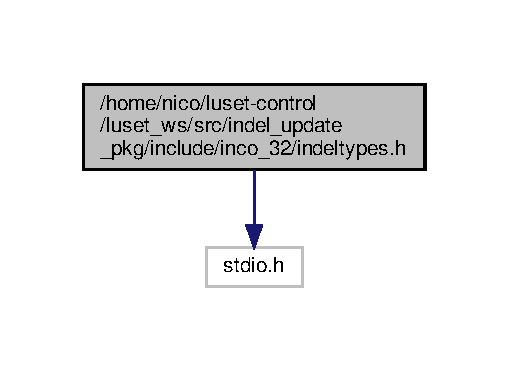
\includegraphics[width=244pt]{indeltypes_8h__incl}
\end{center}
\end{figure}
This graph shows which files directly or indirectly include this file\+:\nopagebreak
\begin{figure}[H]
\begin{center}
\leavevmode
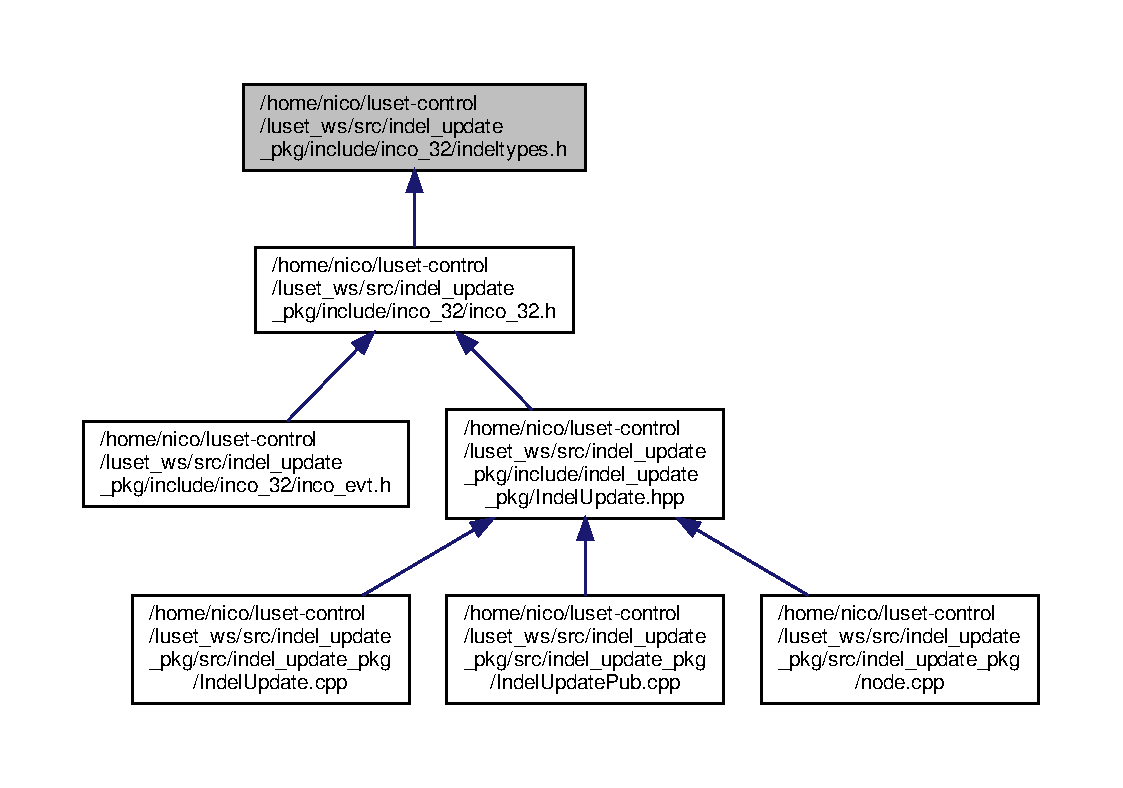
\includegraphics[width=350pt]{indeltypes_8h__dep__incl}
\end{center}
\end{figure}
\subsection*{Macros}
\begin{DoxyCompactItemize}
\item 
\#define \hyperlink{indeltypes_8h_a555bfdbda495f13eee178636428b095c}{U\+LL}(number)~number \#\# U\+I64
\item 
\#define \hyperlink{indeltypes_8h_ad636547d84c568f6472a34ea31dd86e0}{LL}(number)~number \#\# I64
\item 
\#define \hyperlink{indeltypes_8h_a8b0eb8c7522b945921251178487cf272}{L\+O\+N\+G\+L\+O\+N\+G\+F\+O\+R\+M\+AT}~\char`\"{}I64\char`\"{}
\item 
\#define \hyperlink{indeltypes_8h_ac99ec3f1036620727a68aa8c25a8963c}{strcasecmp}~\+\_\+stricmp
\item 
\#define \hyperlink{indeltypes_8h_aba00036f71bb67f8600b239a39cf5ec9}{strncasecmp}~\+\_\+strnicmp
\item 
\#define \hyperlink{indeltypes_8h_aa367b75c5aed883fef5befbdf04835a4}{snprintf}~\+\_\+snprintf
\end{DoxyCompactItemize}
\subsection*{Typedefs}
\begin{DoxyCompactItemize}
\item 
typedef unsigned char \hyperlink{indeltypes_8h_adde6aaee8457bee49c2a92621fe22b79}{uint8}
\item 
typedef signed char \hyperlink{indeltypes_8h_a1b956fe1df85f3c132b21edb4e116458}{int8}
\item 
typedef unsigned short \hyperlink{indeltypes_8h_a05f6b0ae8f6a6e135b0e290c25fe0e4e}{uint16}
\item 
typedef signed short \hyperlink{indeltypes_8h_a259fa4834387bd68627ddf37bb3ebdb9}{int16}
\item 
typedef unsigned long \hyperlink{indeltypes_8h_a4b435a49c74bb91f284f075e63416cb6}{uint32}
\item 
typedef signed long \hyperlink{indeltypes_8h_ac44d0188f4f50fd9b03031c1a06bd0a9}{int32}
\item 
typedef unsigned \+\_\+\+\_\+int64 \hyperlink{indeltypes_8h_ac6afe794ed283c11fb63426a58188e5e}{uint64}
\item 
typedef signed \+\_\+\+\_\+int64 \hyperlink{indeltypes_8h_a0a83e07c3711cb033e7a116fb04c7d3f}{int64}
\item 
typedef \hyperlink{indeltypes_8h_ac44d0188f4f50fd9b03031c1a06bd0a9}{int32} \hyperlink{indeltypes_8h_adb4a1283ff9f4206cf6e92e03a77362f}{intptr}
\item 
typedef \hyperlink{indeltypes_8h_a4b435a49c74bb91f284f075e63416cb6}{uint32} \hyperlink{indeltypes_8h_a90edca57331df76ff61d931bd8f0b52c}{uintptr}
\end{DoxyCompactItemize}


\subsection{Detailed Description}
Not yet described. 

\begin{DoxyAuthor}{Author}
Raphael Zulliger, \copyright{} I\+N\+D\+EL AG 
\end{DoxyAuthor}
\begin{DoxyVersion}{Version}
1.\+00 \begin{DoxyVerb}2322, 2007-12-18 09:15:36 +0100 (Di, 18 Dez 2007), zulliger
! Many many changes. Too much to list in detail. But: A lot of
  McINCOFrame adjustments (especially regarding little/big-endian), a lot
  of cleanups in library structure, etc.

2323, 2007-12-18 10:49:05 +0100 (Di, 18 Dez 2007), zulliger
- Removed obsolete definitions from file

2427, 2008-01-04 11:28:37 +0100 (Fr, 04 Jan 2008), zulliger
- Removed error-clause if neither INDEL_WINDOWS nor INDEL_LINUX is defined.

2474, 2008-02-04 15:29:26 +0100 (Mo, 04 Feb 2008), zulliger
+ Added some commonly useful defs

3995, 2010-02-23 10:21:17 +0100 (Tue, 23 Feb 2010), fabi
! Adjusted to generate java classes with swig.

4292, 2010-07-01 16:49:46 +0200 (Do, 01 Jul 2010), tjericke
Added support for 64bit systems

4294, 2010-07-02 07:32:07 +0200 (Fr, 02 Jul 2010), tjericke
! Don't define ptr_t types for windows projects, they are already defined.

4295, 2010-07-02 09:16:47 +0200 (Fr, 02 Jul 2010), tjericke
! Changed intptr_t and uintptr_t to intptr and uintptr

4296, 2010-07-02 09:42:39 +0200 (Fri, 02 Jul 2010), walther
! Defining macro UL instead of ULL in r4292 was a typo. (We use the same
  definition for both the 32 bit and 64 bit cases to stay true to the name
  of the macro, I guess on an LP64 system using the resulting long long
  constant in a long (int64) context should work fine.)

4383, 2010-07-27 15:00:12 +0200 (Tue, 27 Jul 2010), tjericke
! Changed defines of uint32 and int32 to use int instead of long. On windows the INDEL_NOLONG define 
  has to be set (for backwards compatibility). Otherwise the old definition is used.

4649, 2010-11-15 09:21:07 +0100 (Mo, 15 Nov 2010), zulliger
! Fixed the Linux 64Bit definition of ULL and UL. The error popped up
  because the unittests are now compiled by default when using ibuild.py

4688, 2010-11-26 10:15:36 +0100 (Fr, 26 Nov 2010), fabi
- Removed VC6 workaround.

4987, 2011-10-19 16:13:42 +0200 (Wed, 19 Oct 2011), walther
+ Port libindel to Mac OS X and iOS. Not all parts are implemented, but
  enough to get libinco_32 to work (using TCP). Missing in particular:
  global semaphores, shared-memory communication, network interface
  functions. Linux implementation files that are also used on Mac OS X are
  moved from src/src/linux to src/src/shared. Building for Mac OS X works
  using ibuild.py like on Linux. For iOS, an Xcode project is provided. It
  requires wxWidgets-2.9.2 (unmodified source distribution), placed
  relative to the project as specified by the WXROOT build setting.

5993, 2014-03-10 10:11:42 +0100 (Mon, 10 Mar 2014), zulliger
! Changed inclusion of C++ header file to C header file. This allows using
  the header file for C-only compilers, such as used by Matlab/Simulink to
  access C-DLLs

$LastChangedRevision: 6646 $ $Date: 2016-07-12 10:17:15 +0200 (Tue, 12 Jul 2016) $ $Author: walther $
! Don't define snprintf as _snprintf on MSVC14, which now has a standards-
  compliant implementation. (Using _snprintf as snprintf seems questionable
  anyway, as it behaves differently from what is expected of a snprintf.)

$Comment$

u = unreleased
+ = new feature
! = change, bugfix
- = removed\end{DoxyVerb}

\end{DoxyVersion}
\begin{DoxyRemark}{Remarks}
\begin{DoxyVerb}project         : IndelLib
language        : C++ (Gnu, Visual C++)
system          : Linux, Windows
\end{DoxyVerb}
 
\end{DoxyRemark}


\subsection{Macro Definition Documentation}
\mbox{\Hypertarget{indeltypes_8h_ad636547d84c568f6472a34ea31dd86e0}\label{indeltypes_8h_ad636547d84c568f6472a34ea31dd86e0}} 
\index{indeltypes.\+h@{indeltypes.\+h}!LL@{LL}}
\index{LL@{LL}!indeltypes.\+h@{indeltypes.\+h}}
\subsubsection{\texorpdfstring{LL}{LL}}
{\footnotesize\ttfamily \#define LL(\begin{DoxyParamCaption}\item[{}]{number }\end{DoxyParamCaption})~number \#\# I64}

\mbox{\Hypertarget{indeltypes_8h_a8b0eb8c7522b945921251178487cf272}\label{indeltypes_8h_a8b0eb8c7522b945921251178487cf272}} 
\index{indeltypes.\+h@{indeltypes.\+h}!L\+O\+N\+G\+L\+O\+N\+G\+F\+O\+R\+M\+AT@{L\+O\+N\+G\+L\+O\+N\+G\+F\+O\+R\+M\+AT}}
\index{L\+O\+N\+G\+L\+O\+N\+G\+F\+O\+R\+M\+AT@{L\+O\+N\+G\+L\+O\+N\+G\+F\+O\+R\+M\+AT}!indeltypes.\+h@{indeltypes.\+h}}
\subsubsection{\texorpdfstring{L\+O\+N\+G\+L\+O\+N\+G\+F\+O\+R\+M\+AT}{LONGLONGFORMAT}}
{\footnotesize\ttfamily \#define L\+O\+N\+G\+L\+O\+N\+G\+F\+O\+R\+M\+AT~\char`\"{}I64\char`\"{}}

\mbox{\Hypertarget{indeltypes_8h_aa367b75c5aed883fef5befbdf04835a4}\label{indeltypes_8h_aa367b75c5aed883fef5befbdf04835a4}} 
\index{indeltypes.\+h@{indeltypes.\+h}!snprintf@{snprintf}}
\index{snprintf@{snprintf}!indeltypes.\+h@{indeltypes.\+h}}
\subsubsection{\texorpdfstring{snprintf}{snprintf}}
{\footnotesize\ttfamily \#define snprintf~\+\_\+snprintf}

\mbox{\Hypertarget{indeltypes_8h_ac99ec3f1036620727a68aa8c25a8963c}\label{indeltypes_8h_ac99ec3f1036620727a68aa8c25a8963c}} 
\index{indeltypes.\+h@{indeltypes.\+h}!strcasecmp@{strcasecmp}}
\index{strcasecmp@{strcasecmp}!indeltypes.\+h@{indeltypes.\+h}}
\subsubsection{\texorpdfstring{strcasecmp}{strcasecmp}}
{\footnotesize\ttfamily \#define strcasecmp~\+\_\+stricmp}

\mbox{\Hypertarget{indeltypes_8h_aba00036f71bb67f8600b239a39cf5ec9}\label{indeltypes_8h_aba00036f71bb67f8600b239a39cf5ec9}} 
\index{indeltypes.\+h@{indeltypes.\+h}!strncasecmp@{strncasecmp}}
\index{strncasecmp@{strncasecmp}!indeltypes.\+h@{indeltypes.\+h}}
\subsubsection{\texorpdfstring{strncasecmp}{strncasecmp}}
{\footnotesize\ttfamily \#define strncasecmp~\+\_\+strnicmp}

\mbox{\Hypertarget{indeltypes_8h_a555bfdbda495f13eee178636428b095c}\label{indeltypes_8h_a555bfdbda495f13eee178636428b095c}} 
\index{indeltypes.\+h@{indeltypes.\+h}!U\+LL@{U\+LL}}
\index{U\+LL@{U\+LL}!indeltypes.\+h@{indeltypes.\+h}}
\subsubsection{\texorpdfstring{U\+LL}{ULL}}
{\footnotesize\ttfamily \#define U\+LL(\begin{DoxyParamCaption}\item[{}]{number }\end{DoxyParamCaption})~number \#\# U\+I64}



\subsection{Typedef Documentation}
\mbox{\Hypertarget{indeltypes_8h_a259fa4834387bd68627ddf37bb3ebdb9}\label{indeltypes_8h_a259fa4834387bd68627ddf37bb3ebdb9}} 
\index{indeltypes.\+h@{indeltypes.\+h}!int16@{int16}}
\index{int16@{int16}!indeltypes.\+h@{indeltypes.\+h}}
\subsubsection{\texorpdfstring{int16}{int16}}
{\footnotesize\ttfamily typedef signed short \hyperlink{indeltypes_8h_a259fa4834387bd68627ddf37bb3ebdb9}{int16}}

\mbox{\Hypertarget{indeltypes_8h_ac44d0188f4f50fd9b03031c1a06bd0a9}\label{indeltypes_8h_ac44d0188f4f50fd9b03031c1a06bd0a9}} 
\index{indeltypes.\+h@{indeltypes.\+h}!int32@{int32}}
\index{int32@{int32}!indeltypes.\+h@{indeltypes.\+h}}
\subsubsection{\texorpdfstring{int32}{int32}}
{\footnotesize\ttfamily typedef signed long \hyperlink{indeltypes_8h_ac44d0188f4f50fd9b03031c1a06bd0a9}{int32}}

\mbox{\Hypertarget{indeltypes_8h_a0a83e07c3711cb033e7a116fb04c7d3f}\label{indeltypes_8h_a0a83e07c3711cb033e7a116fb04c7d3f}} 
\index{indeltypes.\+h@{indeltypes.\+h}!int64@{int64}}
\index{int64@{int64}!indeltypes.\+h@{indeltypes.\+h}}
\subsubsection{\texorpdfstring{int64}{int64}}
{\footnotesize\ttfamily typedef signed \+\_\+\+\_\+int64 \hyperlink{indeltypes_8h_a0a83e07c3711cb033e7a116fb04c7d3f}{int64}}

\mbox{\Hypertarget{indeltypes_8h_a1b956fe1df85f3c132b21edb4e116458}\label{indeltypes_8h_a1b956fe1df85f3c132b21edb4e116458}} 
\index{indeltypes.\+h@{indeltypes.\+h}!int8@{int8}}
\index{int8@{int8}!indeltypes.\+h@{indeltypes.\+h}}
\subsubsection{\texorpdfstring{int8}{int8}}
{\footnotesize\ttfamily typedef signed char \hyperlink{indeltypes_8h_a1b956fe1df85f3c132b21edb4e116458}{int8}}

\mbox{\Hypertarget{indeltypes_8h_adb4a1283ff9f4206cf6e92e03a77362f}\label{indeltypes_8h_adb4a1283ff9f4206cf6e92e03a77362f}} 
\index{indeltypes.\+h@{indeltypes.\+h}!intptr@{intptr}}
\index{intptr@{intptr}!indeltypes.\+h@{indeltypes.\+h}}
\subsubsection{\texorpdfstring{intptr}{intptr}}
{\footnotesize\ttfamily typedef \hyperlink{indeltypes_8h_ac44d0188f4f50fd9b03031c1a06bd0a9}{int32} \hyperlink{indeltypes_8h_adb4a1283ff9f4206cf6e92e03a77362f}{intptr}}

\mbox{\Hypertarget{indeltypes_8h_a05f6b0ae8f6a6e135b0e290c25fe0e4e}\label{indeltypes_8h_a05f6b0ae8f6a6e135b0e290c25fe0e4e}} 
\index{indeltypes.\+h@{indeltypes.\+h}!uint16@{uint16}}
\index{uint16@{uint16}!indeltypes.\+h@{indeltypes.\+h}}
\subsubsection{\texorpdfstring{uint16}{uint16}}
{\footnotesize\ttfamily typedef unsigned short \hyperlink{indeltypes_8h_a05f6b0ae8f6a6e135b0e290c25fe0e4e}{uint16}}

\mbox{\Hypertarget{indeltypes_8h_a4b435a49c74bb91f284f075e63416cb6}\label{indeltypes_8h_a4b435a49c74bb91f284f075e63416cb6}} 
\index{indeltypes.\+h@{indeltypes.\+h}!uint32@{uint32}}
\index{uint32@{uint32}!indeltypes.\+h@{indeltypes.\+h}}
\subsubsection{\texorpdfstring{uint32}{uint32}}
{\footnotesize\ttfamily typedef unsigned long \hyperlink{indeltypes_8h_a4b435a49c74bb91f284f075e63416cb6}{uint32}}

\mbox{\Hypertarget{indeltypes_8h_ac6afe794ed283c11fb63426a58188e5e}\label{indeltypes_8h_ac6afe794ed283c11fb63426a58188e5e}} 
\index{indeltypes.\+h@{indeltypes.\+h}!uint64@{uint64}}
\index{uint64@{uint64}!indeltypes.\+h@{indeltypes.\+h}}
\subsubsection{\texorpdfstring{uint64}{uint64}}
{\footnotesize\ttfamily typedef unsigned \+\_\+\+\_\+int64 \hyperlink{indeltypes_8h_ac6afe794ed283c11fb63426a58188e5e}{uint64}}

\mbox{\Hypertarget{indeltypes_8h_adde6aaee8457bee49c2a92621fe22b79}\label{indeltypes_8h_adde6aaee8457bee49c2a92621fe22b79}} 
\index{indeltypes.\+h@{indeltypes.\+h}!uint8@{uint8}}
\index{uint8@{uint8}!indeltypes.\+h@{indeltypes.\+h}}
\subsubsection{\texorpdfstring{uint8}{uint8}}
{\footnotesize\ttfamily typedef unsigned char \hyperlink{indeltypes_8h_adde6aaee8457bee49c2a92621fe22b79}{uint8}}

\mbox{\Hypertarget{indeltypes_8h_a90edca57331df76ff61d931bd8f0b52c}\label{indeltypes_8h_a90edca57331df76ff61d931bd8f0b52c}} 
\index{indeltypes.\+h@{indeltypes.\+h}!uintptr@{uintptr}}
\index{uintptr@{uintptr}!indeltypes.\+h@{indeltypes.\+h}}
\subsubsection{\texorpdfstring{uintptr}{uintptr}}
{\footnotesize\ttfamily typedef \hyperlink{indeltypes_8h_a4b435a49c74bb91f284f075e63416cb6}{uint32} \hyperlink{indeltypes_8h_a90edca57331df76ff61d931bd8f0b52c}{uintptr}}


\hypertarget{IndelUpdate_8hpp}{}\section{/home/nico/luset-\/control/luset\+\_\+ws/src/indel\+\_\+update\+\_\+pkg/include/indel\+\_\+update\+\_\+pkg/\+Indel\+Update.hpp File Reference}
\label{IndelUpdate_8hpp}\index{/home/nico/luset-\/control/luset\+\_\+ws/src/indel\+\_\+update\+\_\+pkg/include/indel\+\_\+update\+\_\+pkg/\+Indel\+Update.\+hpp@{/home/nico/luset-\/control/luset\+\_\+ws/src/indel\+\_\+update\+\_\+pkg/include/indel\+\_\+update\+\_\+pkg/\+Indel\+Update.\+hpp}}


This is the header file for the Indel\+Update class. This class handles communication with the low-\/level controller by calling functions from the Indel inco\+\_\+32.\+so shared library which returns an array of the sensor measurments. This class also publishes the data to the R\+OS topic, /\+Indel\+Update. See \href{https://google.github.io/styleguide/cppguide.html}{\tt https\+://google.\+github.\+io/styleguide/cppguide.\+html} for Google Style Guide for C++.  


{\ttfamily \#include $<$stdio.\+h$>$}\newline
{\ttfamily \#include $<$string.\+h$>$}\newline
{\ttfamily \#include $<$stdlib.\+h$>$}\newline
{\ttfamily \#include $<$math.\+h$>$}\newline
{\ttfamily \#include $<$ctype.\+h$>$}\newline
{\ttfamily \#include $<$time.\+h$>$}\newline
{\ttfamily \#include $<$iostream$>$}\newline
{\ttfamily \#include $<$dlfcn.\+h$>$}\newline
{\ttfamily \#include \char`\"{}inco\+\_\+32/inco\+\_\+32.\+h\char`\"{}}\newline
{\ttfamily \#include \char`\"{}ros/ros.\+h\char`\"{}}\newline
{\ttfamily \#include \char`\"{}indel\+\_\+update\+\_\+pkg/\+Luset\+State\+Array.\+h\char`\"{}}\newline
Include dependency graph for Indel\+Update.\+hpp\+:\nopagebreak
\begin{figure}[H]
\begin{center}
\leavevmode
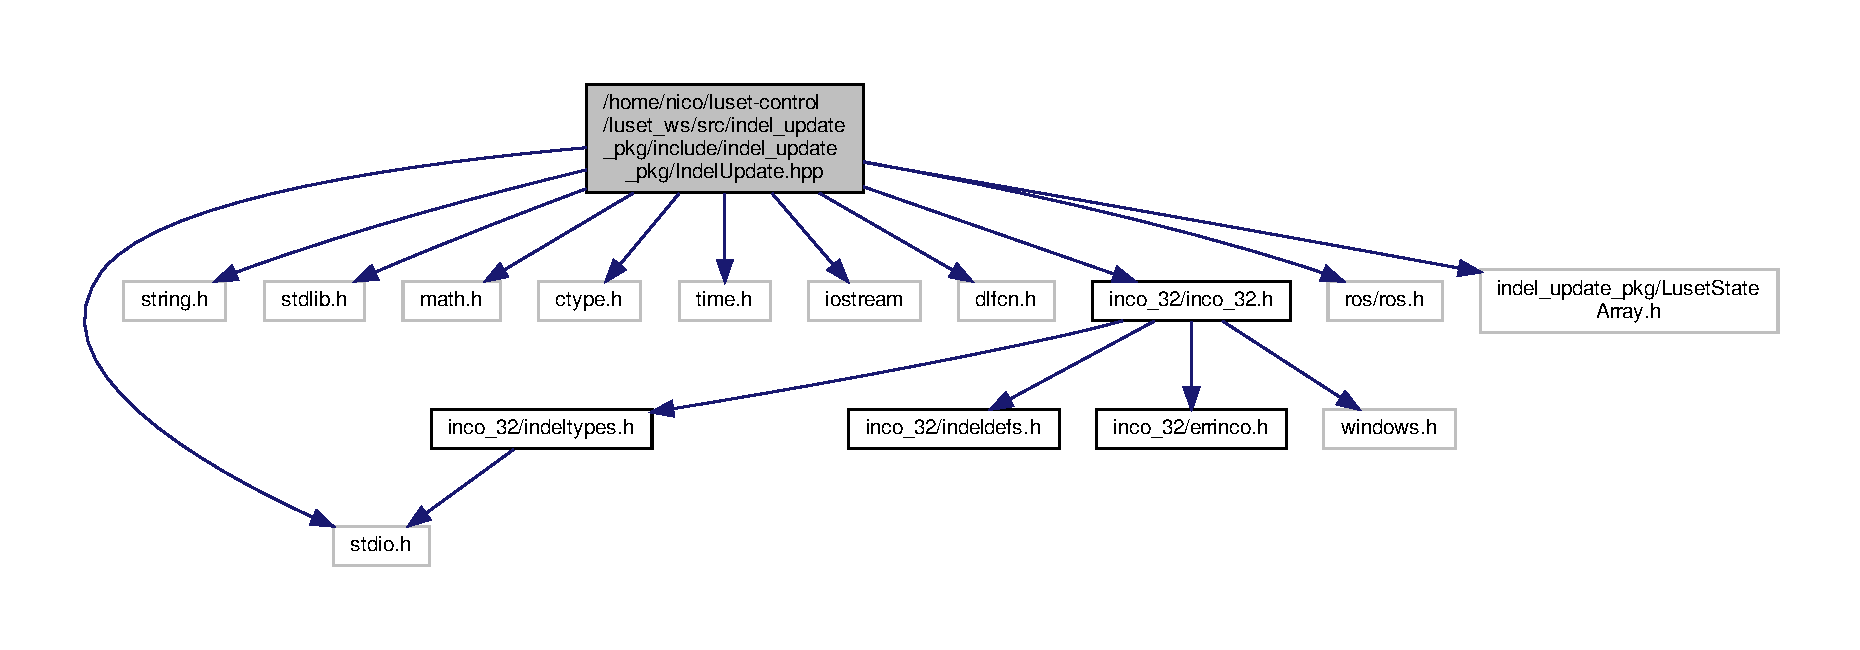
\includegraphics[width=350pt]{IndelUpdate_8hpp__incl}
\end{center}
\end{figure}
This graph shows which files directly or indirectly include this file\+:\nopagebreak
\begin{figure}[H]
\begin{center}
\leavevmode
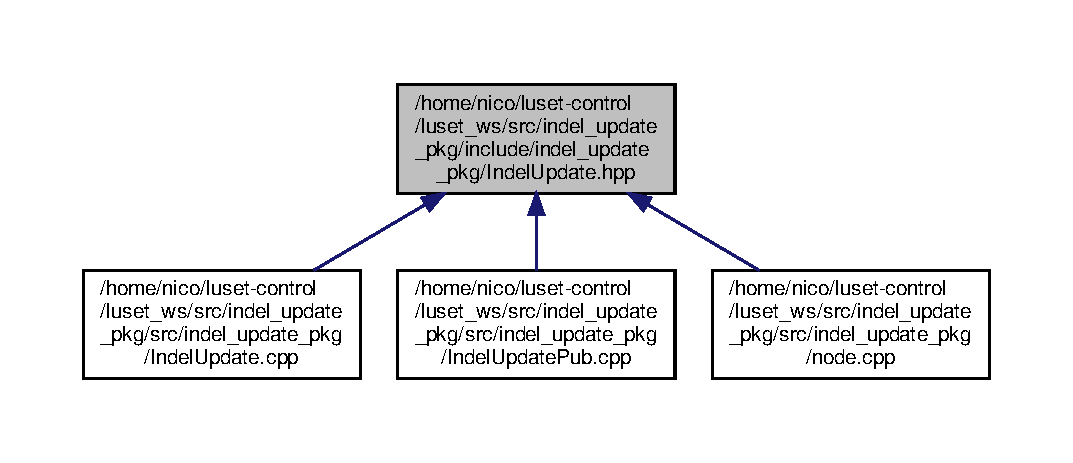
\includegraphics[width=350pt]{IndelUpdate_8hpp__dep__incl}
\end{center}
\end{figure}
\subsection*{Classes}
\begin{DoxyCompactItemize}
\item 
class \hyperlink{classindelupdatenamespace_1_1IndelUpdate}{indelupdatenamespace\+::\+Indel\+Update}
\begin{DoxyCompactList}\small\item\em This class provides the interface between the low-\/level controller and the R\+OS control system. \end{DoxyCompactList}\item 
class \hyperlink{classindelupdatepubnamespace_1_1IndelUpdatePub}{indelupdatepubnamespace\+::\+Indel\+Update\+Pub}
\begin{DoxyCompactList}\small\item\em This class handles publishing to the /\+Indel\+Update topic data acquired from the low-\/level controller. \end{DoxyCompactList}\end{DoxyCompactItemize}
\subsection*{Namespaces}
\begin{DoxyCompactItemize}
\item 
 \hyperlink{namespaceindelupdatenamespace}{indelupdatenamespace}
\item 
 \hyperlink{namespaceindelupdatepubnamespace}{indelupdatepubnamespace}
\end{DoxyCompactItemize}


\subsection{Detailed Description}
This is the header file for the Indel\+Update class. This class handles communication with the low-\/level controller by calling functions from the Indel inco\+\_\+32.\+so shared library which returns an array of the sensor measurments. This class also publishes the data to the R\+OS topic, /\+Indel\+Update. See \href{https://google.github.io/styleguide/cppguide.html}{\tt https\+://google.\+github.\+io/styleguide/cppguide.\+html} for Google Style Guide for C++. 

This is the header file for the Luset\+Control and Luset\+Collision classes. The Luset\+Collision class is responsible for subscribing to the /\+Luset\+State topic and for publishing the actuator strokes to the correct actuators in the Gazebo simulation. It also publishes a message to the /\+Luset\+Contacts topic if a collision between two components in the model is detected. The Luset\+Control class is not yet implemented, but in the future, it will handle the control algorithm (L\+QR, PI, M\+PC, etc.) that computes the axis/valve displacements to send to the low-\/level controller, which interfaces with the Indel\+Update class. See \href{https://google.github.io/styleguide/cppguide.html}{\tt https\+://google.\+github.\+io/styleguide/cppguide.\+html} for Google Style Guide for C++.

\begin{DoxyAuthor}{Author}
Nicholas José Palomo (\href{mailto:npalomo@student.ethz.ch}{\tt npalomo@student.\+ethz.\+ch}) 
\end{DoxyAuthor}
\begin{DoxyVersion}{Version}
0.\+1 
\end{DoxyVersion}
\begin{DoxyDate}{Date}
2020-\/02-\/23
\end{DoxyDate}
\begin{DoxyCopyright}{Copyright}
Copyright (c) 2020 
\end{DoxyCopyright}

\hypertarget{IndelUpdate_8cpp}{}\section{/home/nico/luset-\/control/luset\+\_\+ws/src/indel\+\_\+update\+\_\+pkg/src/indel\+\_\+update\+\_\+pkg/\+Indel\+Update.cpp File Reference}
\label{IndelUpdate_8cpp}\index{/home/nico/luset-\/control/luset\+\_\+ws/src/indel\+\_\+update\+\_\+pkg/src/indel\+\_\+update\+\_\+pkg/\+Indel\+Update.\+cpp@{/home/nico/luset-\/control/luset\+\_\+ws/src/indel\+\_\+update\+\_\+pkg/src/indel\+\_\+update\+\_\+pkg/\+Indel\+Update.\+cpp}}


This is the source code for the Indel\+Update class. See \href{https://google.github.io/styleguide/cppguide.html}{\tt https\+://google.\+github.\+io/styleguide/cppguide.\+html} for Google Style Guide for C++.  


{\ttfamily \#include \char`\"{}Indel\+Update.\+hpp\char`\"{}}\newline
Include dependency graph for Indel\+Update.\+cpp\+:\nopagebreak
\begin{figure}[H]
\begin{center}
\leavevmode
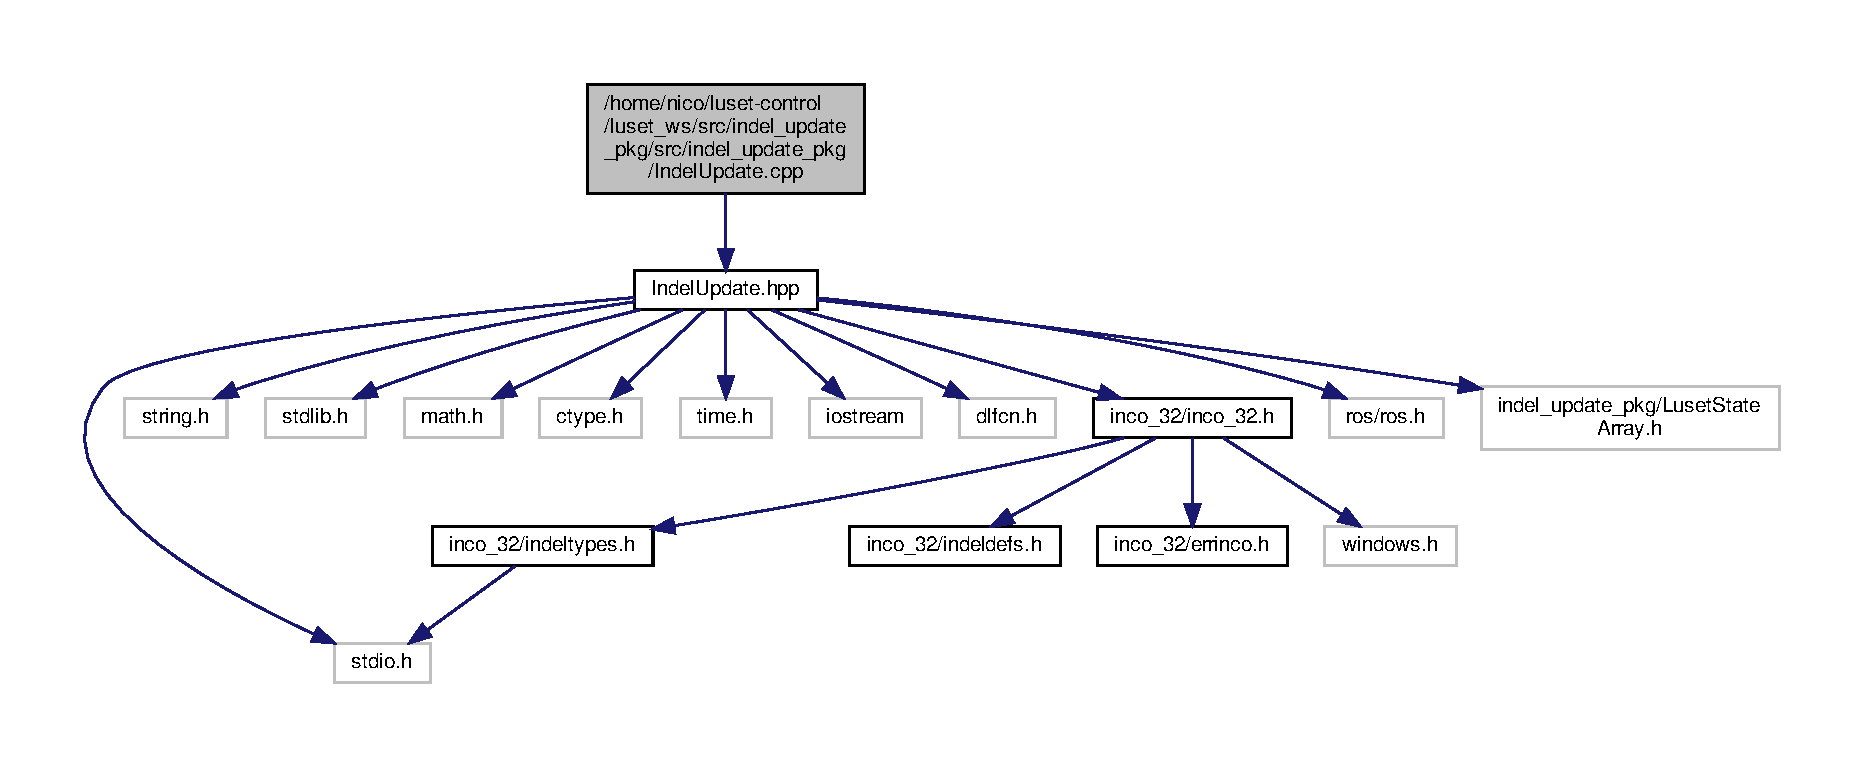
\includegraphics[width=350pt]{IndelUpdate_8cpp__incl}
\end{center}
\end{figure}


\subsection{Detailed Description}
This is the source code for the Indel\+Update class. See \href{https://google.github.io/styleguide/cppguide.html}{\tt https\+://google.\+github.\+io/styleguide/cppguide.\+html} for Google Style Guide for C++. 

\begin{DoxyAuthor}{Author}
Nicholas José Palomo (\href{mailto:npalomo@student.ethz.ch}{\tt npalomo@student.\+ethz.\+ch}) 
\end{DoxyAuthor}
\begin{DoxyVersion}{Version}
0.\+1 
\end{DoxyVersion}
\begin{DoxyDate}{Date}
2020-\/02-\/24
\end{DoxyDate}
\begin{DoxyCopyright}{Copyright}
Copyright (c) 2020 
\end{DoxyCopyright}

\hypertarget{IndelUpdatePub_8cpp}{}\section{/home/nico/luset-\/control/luset\+\_\+ws/src/indel\+\_\+update\+\_\+pkg/src/indel\+\_\+update\+\_\+pkg/\+Indel\+Update\+Pub.cpp File Reference}
\label{IndelUpdatePub_8cpp}\index{/home/nico/luset-\/control/luset\+\_\+ws/src/indel\+\_\+update\+\_\+pkg/src/indel\+\_\+update\+\_\+pkg/\+Indel\+Update\+Pub.\+cpp@{/home/nico/luset-\/control/luset\+\_\+ws/src/indel\+\_\+update\+\_\+pkg/src/indel\+\_\+update\+\_\+pkg/\+Indel\+Update\+Pub.\+cpp}}


This is the source code for the Indel\+Update\+Pub class. See \href{https://google.github.io/styleguide/cppguide.html}{\tt https\+://google.\+github.\+io/styleguide/cppguide.\+html} for Google Style Guide for C++.  


{\ttfamily \#include \char`\"{}Indel\+Update.\+hpp\char`\"{}}\newline
Include dependency graph for Indel\+Update\+Pub.\+cpp\+:\nopagebreak
\begin{figure}[H]
\begin{center}
\leavevmode
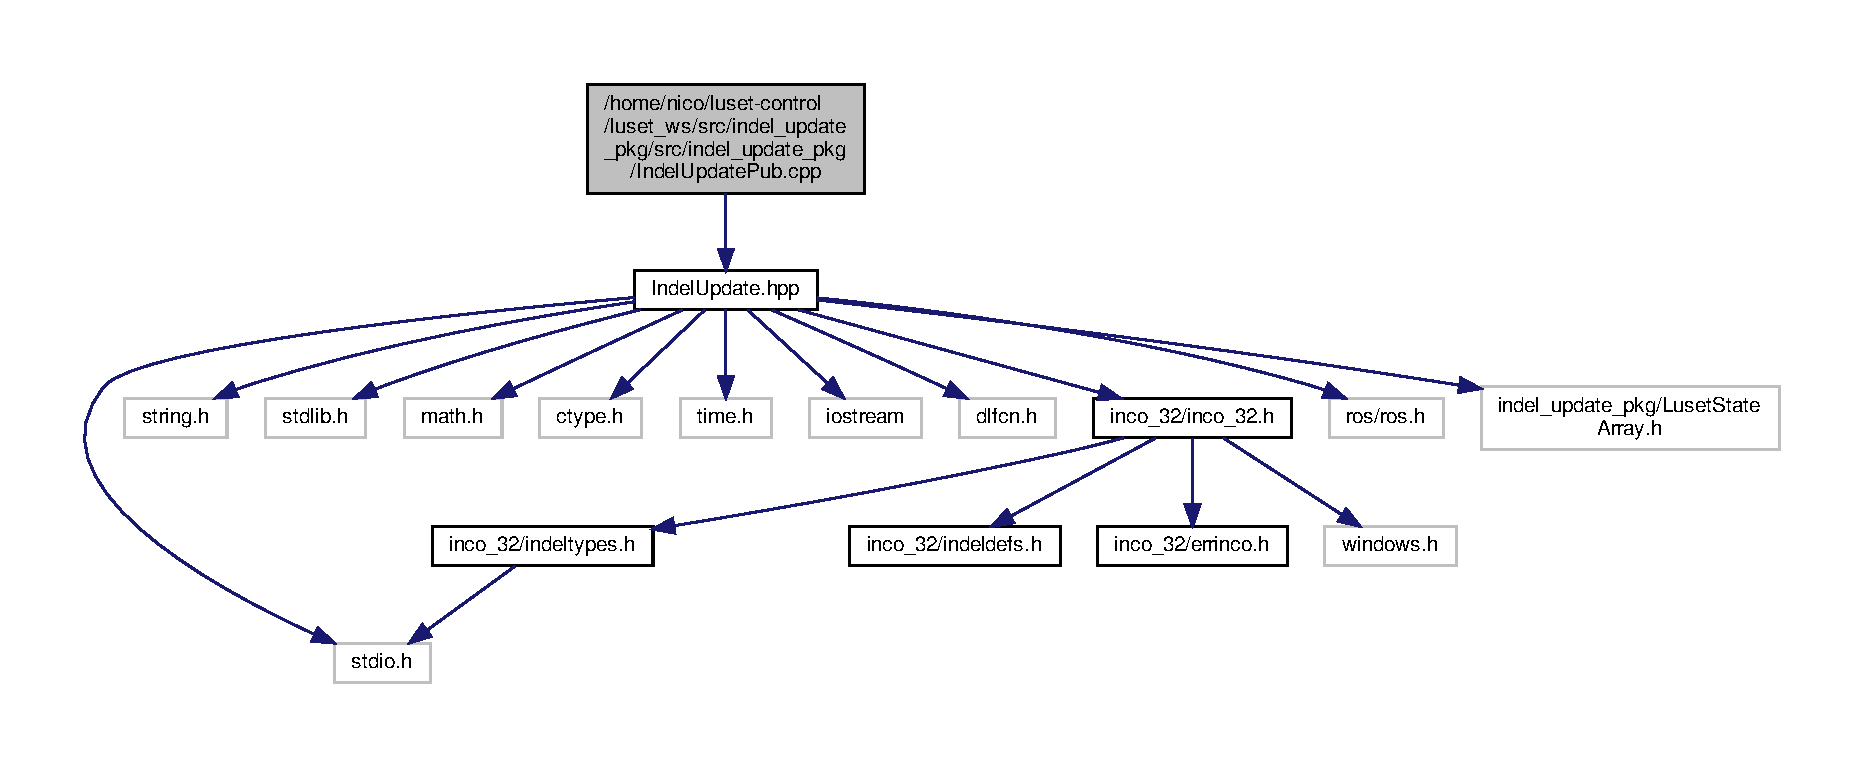
\includegraphics[width=350pt]{IndelUpdatePub_8cpp__incl}
\end{center}
\end{figure}


\subsection{Detailed Description}
This is the source code for the Indel\+Update\+Pub class. See \href{https://google.github.io/styleguide/cppguide.html}{\tt https\+://google.\+github.\+io/styleguide/cppguide.\+html} for Google Style Guide for C++. 

\begin{DoxyAuthor}{Author}
Nicholas José Palomo (\href{mailto:npalomo@student.ethz.ch}{\tt npalomo@student.\+ethz.\+ch}) 
\end{DoxyAuthor}
\begin{DoxyVersion}{Version}
0.\+1 
\end{DoxyVersion}
\begin{DoxyDate}{Date}
2020-\/02-\/24
\end{DoxyDate}
\begin{DoxyCopyright}{Copyright}
Copyright (c) 2020 
\end{DoxyCopyright}

\hypertarget{indel__update__pkg_2src_2indel__update__pkg_2node_8cpp}{}\section{/home/nico/luset-\/control/luset\+\_\+ws/src/indel\+\_\+update\+\_\+pkg/src/indel\+\_\+update\+\_\+pkg/node.cpp File Reference}
\label{indel__update__pkg_2src_2indel__update__pkg_2node_8cpp}\index{/home/nico/luset-\/control/luset\+\_\+ws/src/indel\+\_\+update\+\_\+pkg/src/indel\+\_\+update\+\_\+pkg/node.\+cpp@{/home/nico/luset-\/control/luset\+\_\+ws/src/indel\+\_\+update\+\_\+pkg/src/indel\+\_\+update\+\_\+pkg/node.\+cpp}}
{\ttfamily \#include \char`\"{}Indel\+Update.\+hpp\char`\"{}}\newline
Include dependency graph for node.\+cpp\+:\nopagebreak
\begin{figure}[H]
\begin{center}
\leavevmode
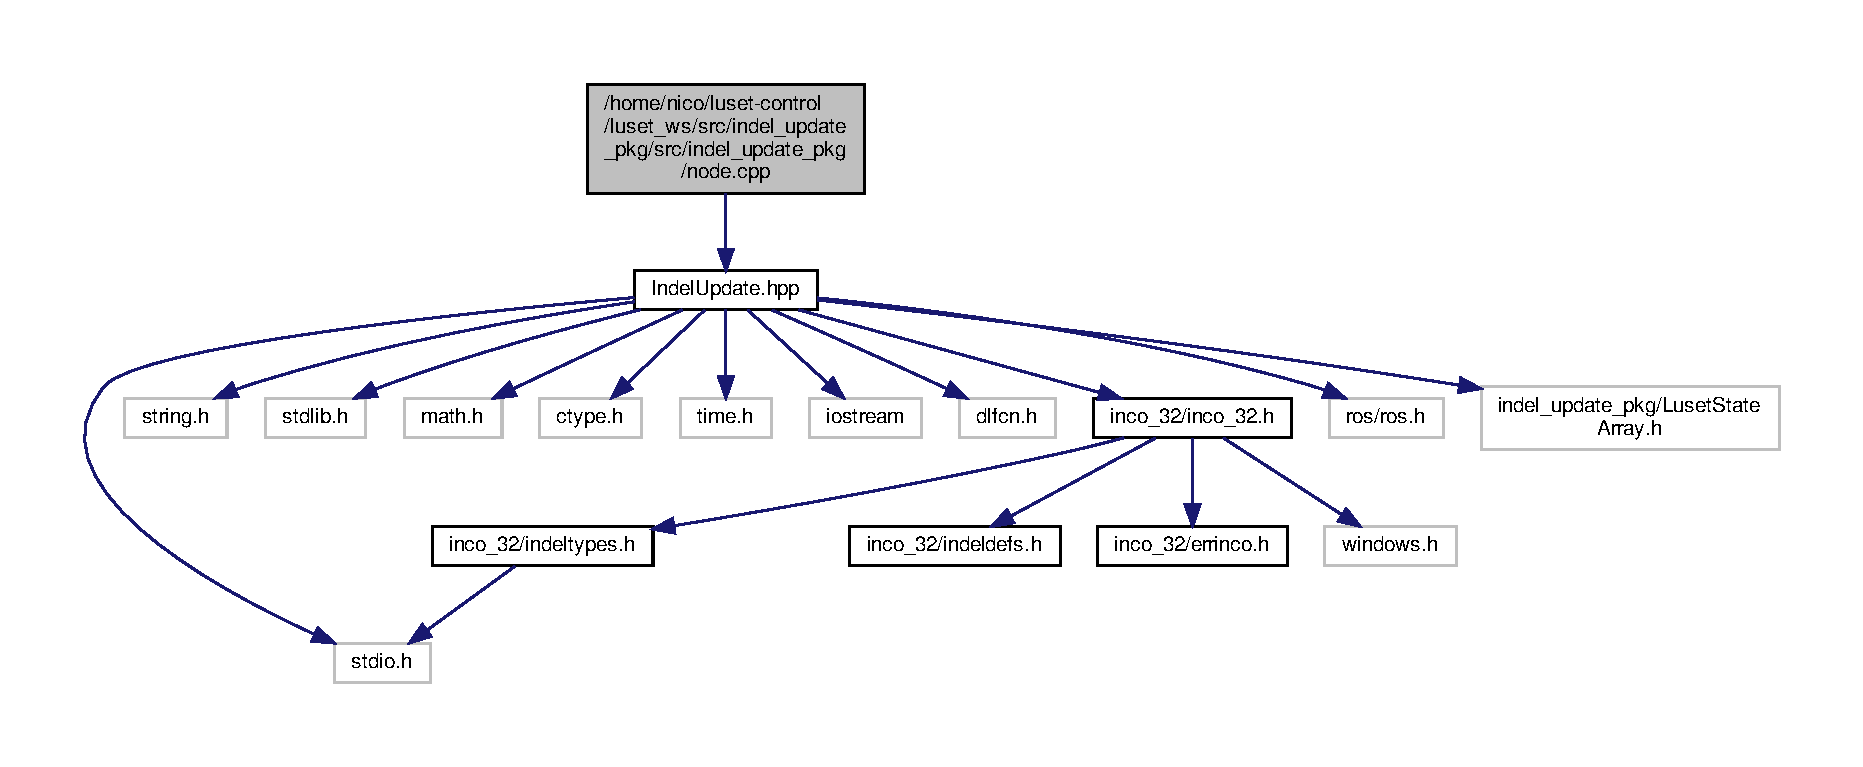
\includegraphics[width=350pt]{indel__update__pkg_2src_2indel__update__pkg_2node_8cpp__incl}
\end{center}
\end{figure}
\subsection*{Functions}
\begin{DoxyCompactItemize}
\item 
int \hyperlink{indel__update__pkg_2src_2indel__update__pkg_2node_8cpp_a3c04138a5bfe5d72780bb7e82a18e627}{main} (int argc, char $\ast$$\ast$argv)
\end{DoxyCompactItemize}


\subsection{Function Documentation}
\mbox{\Hypertarget{indel__update__pkg_2src_2indel__update__pkg_2node_8cpp_a3c04138a5bfe5d72780bb7e82a18e627}\label{indel__update__pkg_2src_2indel__update__pkg_2node_8cpp_a3c04138a5bfe5d72780bb7e82a18e627}} 
\index{indel\+\_\+update\+\_\+pkg/src/indel\+\_\+update\+\_\+pkg/node.\+cpp@{indel\+\_\+update\+\_\+pkg/src/indel\+\_\+update\+\_\+pkg/node.\+cpp}!main@{main}}
\index{main@{main}!indel\+\_\+update\+\_\+pkg/src/indel\+\_\+update\+\_\+pkg/node.\+cpp@{indel\+\_\+update\+\_\+pkg/src/indel\+\_\+update\+\_\+pkg/node.\+cpp}}
\subsubsection{\texorpdfstring{main()}{main()}}
{\footnotesize\ttfamily int main (\begin{DoxyParamCaption}\item[{int}]{argc,  }\item[{char $\ast$$\ast$}]{argv }\end{DoxyParamCaption})}

$<$ Must call ros\+::init() before using any other part of the R\+OS system

$<$ Instantiate a R\+OS node handle

$<$ Set the loop\+\_\+rate for processing the callbacks

$<$ Instantiate Indel\+Update\+Pub object

$<$ Infinite loop until the user shuts down the rosmaster with Ctrl + C

$<$ Call functions to query data from low-\/level controller and to publish to /\+Indel\+Update topic

$<$ ros\+::spin\+Once() processes our callbacks for a single thread; not necessary in this node since there are no subscriber callbacks but added in case functionality added in the future (e.\+g. sending data from other R\+OS topics to low-\/level controller).

$<$ Sleep for the remainder of the loop once all callbacks have been processed. 
\hypertarget{luset__control__pkg_2src_2luset__control__pkg_2node_8cpp}{}\section{/home/nico/luset-\/control/luset\+\_\+ws/src/luset\+\_\+control\+\_\+pkg/src/luset\+\_\+control\+\_\+pkg/node.cpp File Reference}
\label{luset__control__pkg_2src_2luset__control__pkg_2node_8cpp}\index{/home/nico/luset-\/control/luset\+\_\+ws/src/luset\+\_\+control\+\_\+pkg/src/luset\+\_\+control\+\_\+pkg/node.\+cpp@{/home/nico/luset-\/control/luset\+\_\+ws/src/luset\+\_\+control\+\_\+pkg/src/luset\+\_\+control\+\_\+pkg/node.\+cpp}}
{\ttfamily \#include \char`\"{}Luset\+Control.\+hpp\char`\"{}}\newline
Include dependency graph for node.\+cpp\+:\nopagebreak
\begin{figure}[H]
\begin{center}
\leavevmode
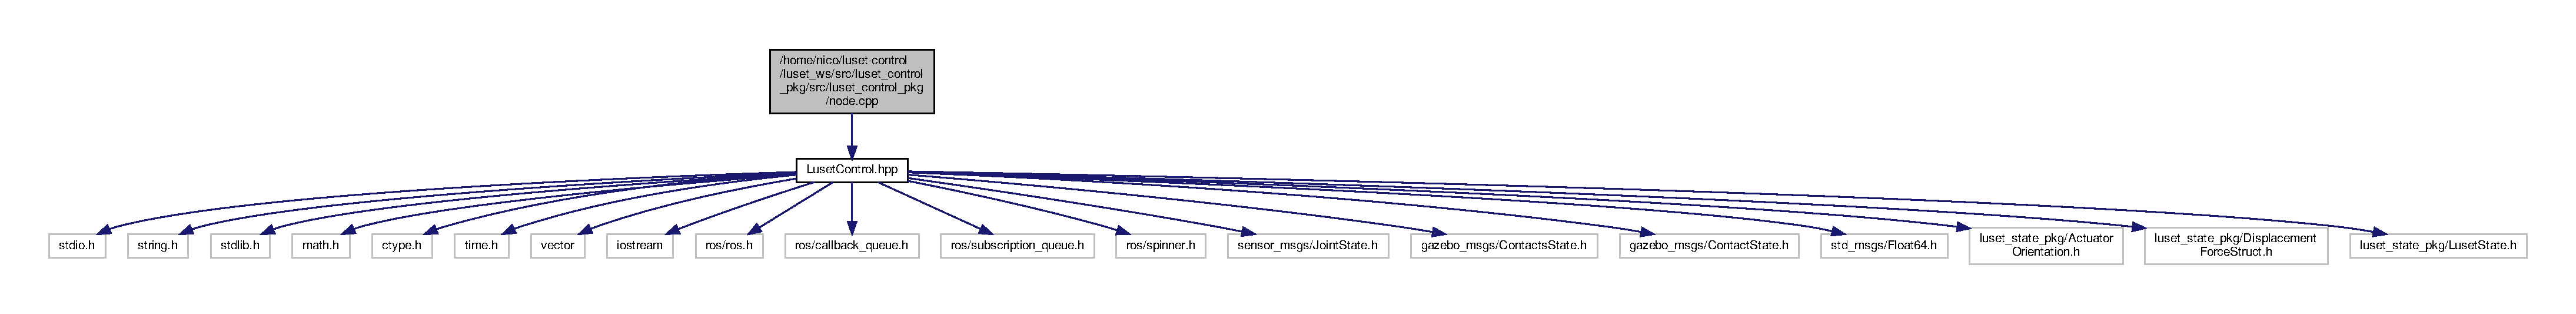
\includegraphics[width=350pt]{luset__control__pkg_2src_2luset__control__pkg_2node_8cpp__incl}
\end{center}
\end{figure}
\subsection*{Functions}
\begin{DoxyCompactItemize}
\item 
int \hyperlink{luset__control__pkg_2src_2luset__control__pkg_2node_8cpp_a3c04138a5bfe5d72780bb7e82a18e627}{main} (int argc, char $\ast$$\ast$argv)
\end{DoxyCompactItemize}


\subsection{Function Documentation}
\mbox{\Hypertarget{luset__control__pkg_2src_2luset__control__pkg_2node_8cpp_a3c04138a5bfe5d72780bb7e82a18e627}\label{luset__control__pkg_2src_2luset__control__pkg_2node_8cpp_a3c04138a5bfe5d72780bb7e82a18e627}} 
\index{luset\+\_\+control\+\_\+pkg/src/luset\+\_\+control\+\_\+pkg/node.\+cpp@{luset\+\_\+control\+\_\+pkg/src/luset\+\_\+control\+\_\+pkg/node.\+cpp}!main@{main}}
\index{main@{main}!luset\+\_\+control\+\_\+pkg/src/luset\+\_\+control\+\_\+pkg/node.\+cpp@{luset\+\_\+control\+\_\+pkg/src/luset\+\_\+control\+\_\+pkg/node.\+cpp}}
\subsubsection{\texorpdfstring{main()}{main()}}
{\footnotesize\ttfamily int main (\begin{DoxyParamCaption}\item[{int}]{argc,  }\item[{char $\ast$$\ast$}]{argv }\end{DoxyParamCaption})}

$<$ Must call ros\+::init() before using any other part of the R\+OS system

$<$ Instantiate a R\+OS node handle

$<$ Instantiate an Async\+Spinner object for the global callback queue (where we process the callback for /\+Luset\+State messages)

$<$ Set the loop\+\_\+rate for processing the callbacks

$<$ Instantiate Luset\+Collision object

$<$ Infinite loop until the user shuts down the rosmaster with Ctrl + C

$<$ Spin multithreaded spinners

$<$ Spin the multithread spinner for the global callback queue

$<$ Only process one callback from the global callback queue

$<$ Sleep for the remainder of the loop once all callbacks have been processed. 
\hypertarget{luset__state__pkg_2src_2luset__state__package_2node_8cpp}{}\section{/home/nico/luset-\/control/luset\+\_\+ws/src/luset\+\_\+state\+\_\+pkg/src/luset\+\_\+state\+\_\+package/node.cpp File Reference}
\label{luset__state__pkg_2src_2luset__state__package_2node_8cpp}\index{/home/nico/luset-\/control/luset\+\_\+ws/src/luset\+\_\+state\+\_\+pkg/src/luset\+\_\+state\+\_\+package/node.\+cpp@{/home/nico/luset-\/control/luset\+\_\+ws/src/luset\+\_\+state\+\_\+pkg/src/luset\+\_\+state\+\_\+package/node.\+cpp}}
{\ttfamily \#include \char`\"{}Luset\+State.\+hpp\char`\"{}}\newline
Include dependency graph for node.\+cpp\+:\nopagebreak
\begin{figure}[H]
\begin{center}
\leavevmode
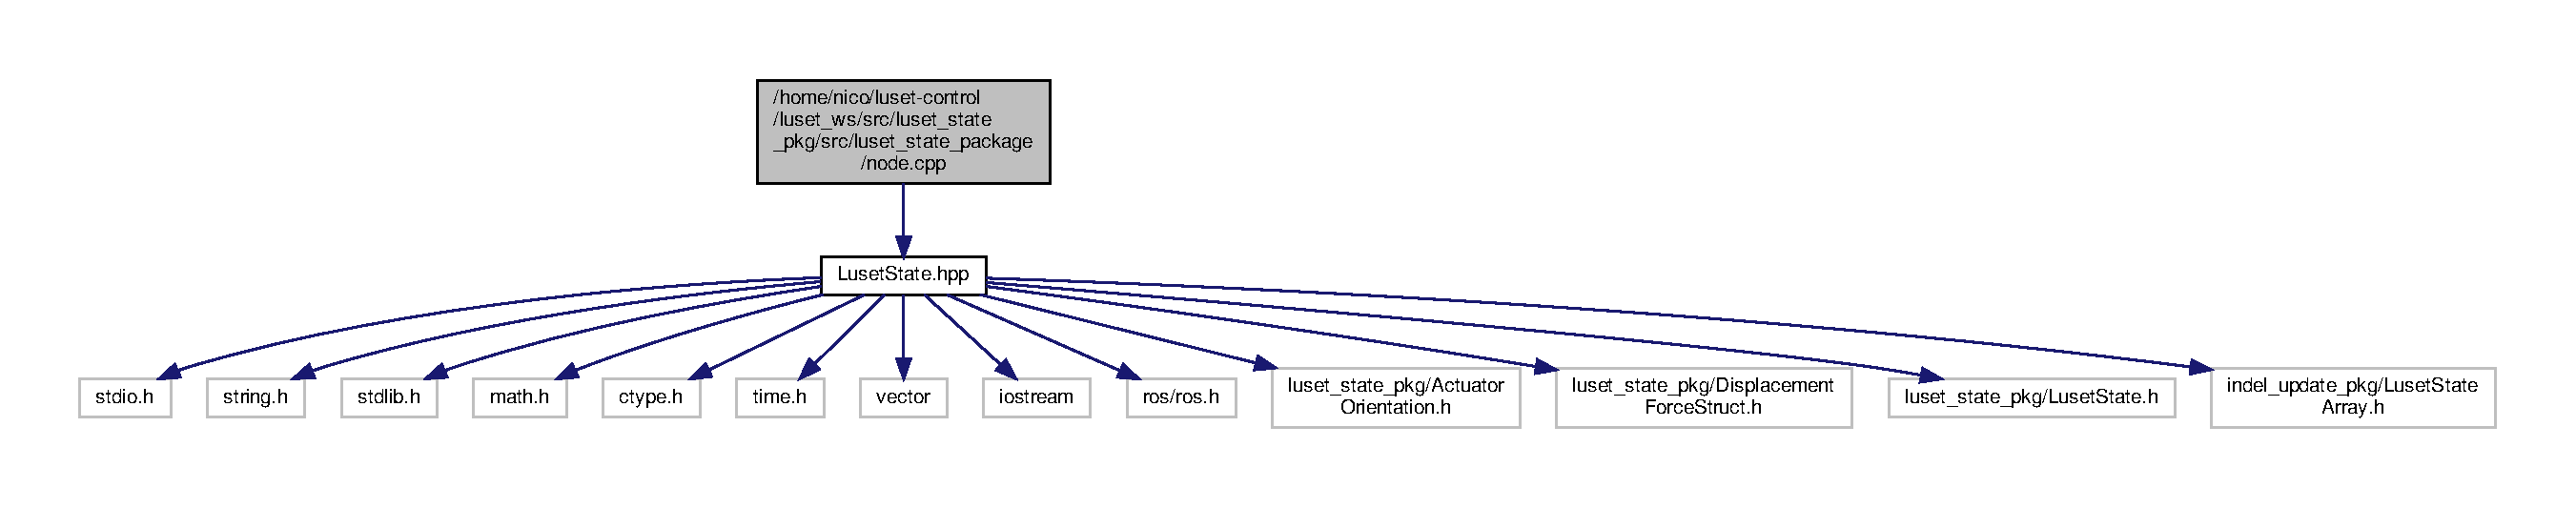
\includegraphics[width=350pt]{luset__state__pkg_2src_2luset__state__package_2node_8cpp__incl}
\end{center}
\end{figure}
\subsection*{Functions}
\begin{DoxyCompactItemize}
\item 
int \hyperlink{luset__state__pkg_2src_2luset__state__package_2node_8cpp_a3c04138a5bfe5d72780bb7e82a18e627}{main} (int argc, char $\ast$$\ast$argv)
\end{DoxyCompactItemize}


\subsection{Function Documentation}
\mbox{\Hypertarget{luset__state__pkg_2src_2luset__state__package_2node_8cpp_a3c04138a5bfe5d72780bb7e82a18e627}\label{luset__state__pkg_2src_2luset__state__package_2node_8cpp_a3c04138a5bfe5d72780bb7e82a18e627}} 
\index{luset\+\_\+state\+\_\+pkg/src/luset\+\_\+state\+\_\+package/node.\+cpp@{luset\+\_\+state\+\_\+pkg/src/luset\+\_\+state\+\_\+package/node.\+cpp}!main@{main}}
\index{main@{main}!luset\+\_\+state\+\_\+pkg/src/luset\+\_\+state\+\_\+package/node.\+cpp@{luset\+\_\+state\+\_\+pkg/src/luset\+\_\+state\+\_\+package/node.\+cpp}}
\subsubsection{\texorpdfstring{main()}{main()}}
{\footnotesize\ttfamily int main (\begin{DoxyParamCaption}\item[{int}]{argc,  }\item[{char $\ast$$\ast$}]{argv }\end{DoxyParamCaption})}

$<$ Must call ros\+::init() before using any other part of the R\+OS system

$<$ Instantiate a R\+OS node handle

$<$ Set the loop\+\_\+rate for processing the callbacks

$<$ Instantiate Luset\+State\+Sub\+Pub object

$<$ Infinite loop until the user shuts down the rosmaster with Ctrl + C

$<$ ros\+::spin\+Once() processes our callbacks for a single thread.

$<$ Sleep for the remainder of the loop once all callbacks have been processed. 
\hypertarget{LusetControl_8hpp}{}\section{/home/nico/luset-\/control/luset\+\_\+ws/src/luset\+\_\+control\+\_\+pkg/include/luset\+\_\+control\+\_\+pkg/\+Luset\+Control.hpp File Reference}
\label{LusetControl_8hpp}\index{/home/nico/luset-\/control/luset\+\_\+ws/src/luset\+\_\+control\+\_\+pkg/include/luset\+\_\+control\+\_\+pkg/\+Luset\+Control.\+hpp@{/home/nico/luset-\/control/luset\+\_\+ws/src/luset\+\_\+control\+\_\+pkg/include/luset\+\_\+control\+\_\+pkg/\+Luset\+Control.\+hpp}}
{\ttfamily \#include $<$stdio.\+h$>$}\newline
{\ttfamily \#include $<$string.\+h$>$}\newline
{\ttfamily \#include $<$stdlib.\+h$>$}\newline
{\ttfamily \#include $<$math.\+h$>$}\newline
{\ttfamily \#include $<$ctype.\+h$>$}\newline
{\ttfamily \#include $<$time.\+h$>$}\newline
{\ttfamily \#include $<$vector$>$}\newline
{\ttfamily \#include $<$iostream$>$}\newline
{\ttfamily \#include \char`\"{}ros/ros.\+h\char`\"{}}\newline
{\ttfamily \#include $<$ros/callback\+\_\+queue.\+h$>$}\newline
{\ttfamily \#include $<$ros/subscription\+\_\+queue.\+h$>$}\newline
{\ttfamily \#include $<$ros/spinner.\+h$>$}\newline
{\ttfamily \#include $<$sensor\+\_\+msgs/\+Joint\+State.\+h$>$}\newline
{\ttfamily \#include $<$gazebo\+\_\+msgs/\+Contacts\+State.\+h$>$}\newline
{\ttfamily \#include $<$gazebo\+\_\+msgs/\+Contact\+State.\+h$>$}\newline
{\ttfamily \#include $<$std\+\_\+msgs/\+Float64.\+h$>$}\newline
{\ttfamily \#include \char`\"{}luset\+\_\+state\+\_\+pkg/\+Actuator\+Orientation.\+h\char`\"{}}\newline
{\ttfamily \#include \char`\"{}luset\+\_\+state\+\_\+pkg/\+Displacement\+Force\+Struct.\+h\char`\"{}}\newline
{\ttfamily \#include \char`\"{}luset\+\_\+state\+\_\+pkg/\+Luset\+State.\+h\char`\"{}}\newline
Include dependency graph for Luset\+Control.\+hpp\+:\nopagebreak
\begin{figure}[H]
\begin{center}
\leavevmode
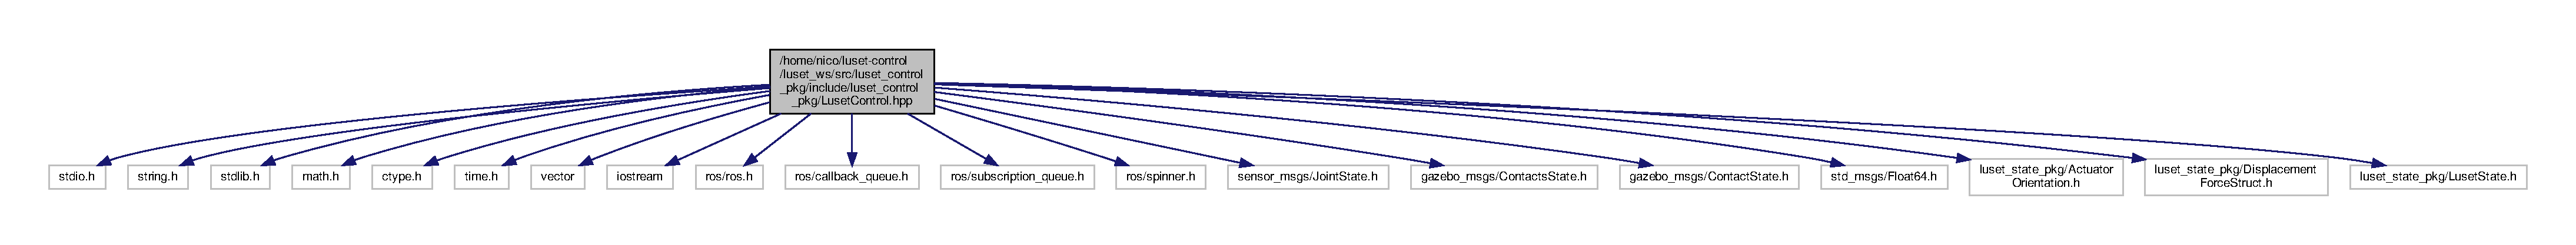
\includegraphics[width=350pt]{LusetControl_8hpp__incl}
\end{center}
\end{figure}
This graph shows which files directly or indirectly include this file\+:\nopagebreak
\begin{figure}[H]
\begin{center}
\leavevmode
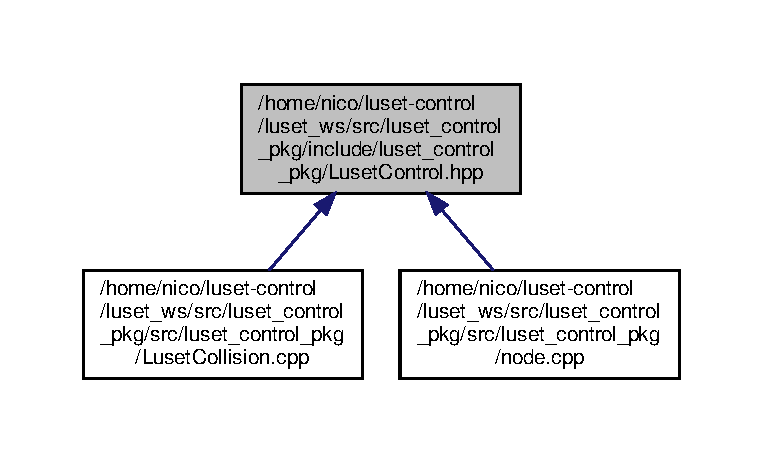
\includegraphics[width=350pt]{LusetControl_8hpp__dep__incl}
\end{center}
\end{figure}
\subsection*{Classes}
\begin{DoxyCompactItemize}
\item 
class \hyperlink{classlusetcontrolnamespace_1_1LusetControl}{lusetcontrolnamespace\+::\+Luset\+Control}
\item 
class \hyperlink{classlusetcontrolnamespace_1_1LusetCollision}{lusetcontrolnamespace\+::\+Luset\+Collision}
\begin{DoxyCompactList}\small\item\em This class subscribes to /\+Luset\+State and publishes the cylinder strokes to the correct cylinders in the Gazebo simulation using information from the parameter server regarding which actuators are connected to the corresponding axes/valves. The values on the parameter server are loaded from /luset\+\_\+control\+\_\+pkg/config/luset\+\_\+valve\+\_\+config\+\_\+standard.yaml. This class also subscribes to the contact sensors in Gazebo publishing on the sensor\+\_\+state topics and only publishes a message to /\+Luset\+Contacts if two components actually collide in the simulation. \end{DoxyCompactList}\end{DoxyCompactItemize}
\subsection*{Namespaces}
\begin{DoxyCompactItemize}
\item 
 \hyperlink{namespacelusetcontrolnamespace}{lusetcontrolnamespace}
\begin{DoxyCompactList}\small\item\em $<$ Used as a stream of Input and Output. \end{DoxyCompactList}\end{DoxyCompactItemize}

\hypertarget{LusetCollision_8cpp}{}\section{/home/nico/luset-\/control/luset\+\_\+ws/src/luset\+\_\+control\+\_\+pkg/src/luset\+\_\+control\+\_\+pkg/\+Luset\+Collision.cpp File Reference}
\label{LusetCollision_8cpp}\index{/home/nico/luset-\/control/luset\+\_\+ws/src/luset\+\_\+control\+\_\+pkg/src/luset\+\_\+control\+\_\+pkg/\+Luset\+Collision.\+cpp@{/home/nico/luset-\/control/luset\+\_\+ws/src/luset\+\_\+control\+\_\+pkg/src/luset\+\_\+control\+\_\+pkg/\+Luset\+Collision.\+cpp}}


This is the source code for the Luset\+Collision class. See \href{https://google.github.io/styleguide/cppguide.html}{\tt https\+://google.\+github.\+io/styleguide/cppguide.\+html} for Google Style Guide for C++.  


{\ttfamily \#include \char`\"{}Luset\+Control.\+hpp\char`\"{}}\newline
Include dependency graph for Luset\+Collision.\+cpp\+:\nopagebreak
\begin{figure}[H]
\begin{center}
\leavevmode
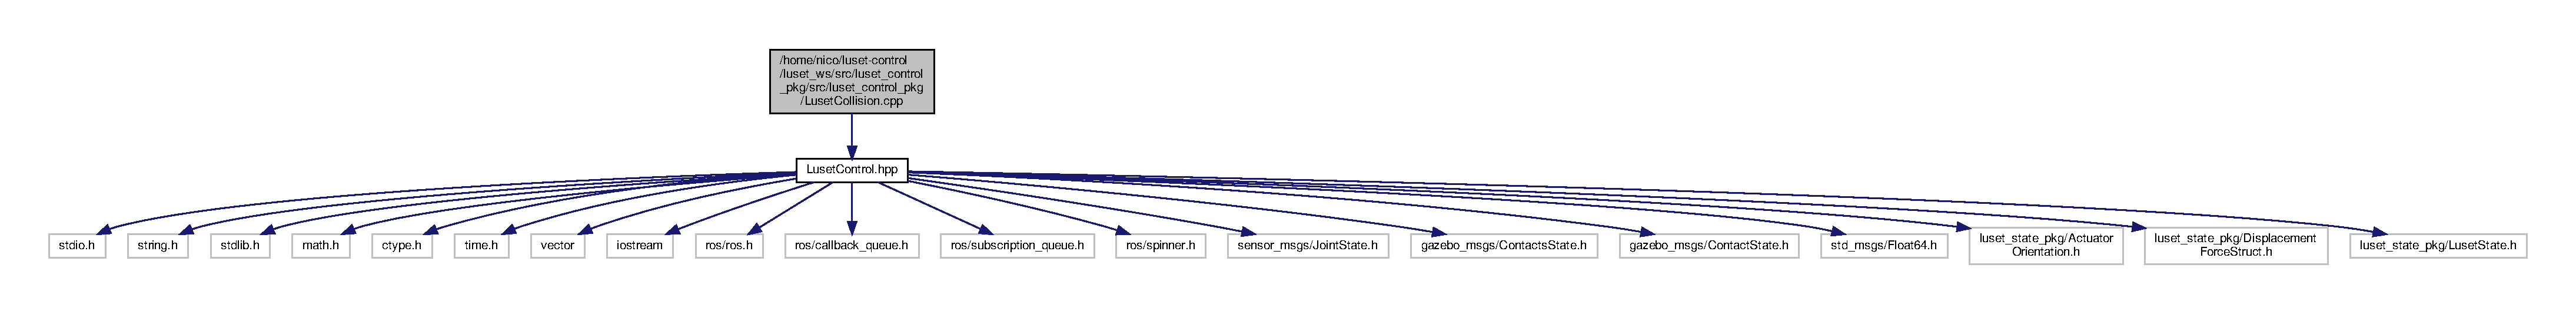
\includegraphics[width=350pt]{LusetCollision_8cpp__incl}
\end{center}
\end{figure}


\subsection{Detailed Description}
This is the source code for the Luset\+Collision class. See \href{https://google.github.io/styleguide/cppguide.html}{\tt https\+://google.\+github.\+io/styleguide/cppguide.\+html} for Google Style Guide for C++. 

\begin{DoxyAuthor}{Author}
Nicholas José Palomo (\href{mailto:npalomo@student.ethz.ch}{\tt npalomo@student.\+ethz.\+ch}) 
\end{DoxyAuthor}
\begin{DoxyVersion}{Version}
0.\+1 
\end{DoxyVersion}
\begin{DoxyDate}{Date}
2020-\/02-\/24
\end{DoxyDate}
\begin{DoxyCopyright}{Copyright}
Copyright (c) 2020 
\end{DoxyCopyright}

\hypertarget{LusetState_8hpp}{}\section{/home/nico/luset-\/control/luset\+\_\+ws/src/luset\+\_\+state\+\_\+pkg/include/luset\+\_\+state\+\_\+pkg/\+Luset\+State.hpp File Reference}
\label{LusetState_8hpp}\index{/home/nico/luset-\/control/luset\+\_\+ws/src/luset\+\_\+state\+\_\+pkg/include/luset\+\_\+state\+\_\+pkg/\+Luset\+State.\+hpp@{/home/nico/luset-\/control/luset\+\_\+ws/src/luset\+\_\+state\+\_\+pkg/include/luset\+\_\+state\+\_\+pkg/\+Luset\+State.\+hpp}}


This is the header file for the Luset\+State and Luset\+State\+Pub classes. See \href{https://google.github.io/styleguide/cppguide.html}{\tt https\+://google.\+github.\+io/styleguide/cppguide.\+html} for Google Style Guide for C++.  


{\ttfamily \#include $<$stdio.\+h$>$}\newline
{\ttfamily \#include $<$string.\+h$>$}\newline
{\ttfamily \#include $<$stdlib.\+h$>$}\newline
{\ttfamily \#include $<$math.\+h$>$}\newline
{\ttfamily \#include $<$ctype.\+h$>$}\newline
{\ttfamily \#include $<$time.\+h$>$}\newline
{\ttfamily \#include $<$vector$>$}\newline
{\ttfamily \#include $<$iostream$>$}\newline
{\ttfamily \#include \char`\"{}ros/ros.\+h\char`\"{}}\newline
{\ttfamily \#include \char`\"{}luset\+\_\+state\+\_\+pkg/\+Actuator\+Orientation.\+h\char`\"{}}\newline
{\ttfamily \#include \char`\"{}luset\+\_\+state\+\_\+pkg/\+Displacement\+Force\+Struct.\+h\char`\"{}}\newline
{\ttfamily \#include \char`\"{}luset\+\_\+state\+\_\+pkg/\+Luset\+State.\+h\char`\"{}}\newline
{\ttfamily \#include \char`\"{}indel\+\_\+update\+\_\+pkg/\+Luset\+State\+Array.\+h\char`\"{}}\newline
Include dependency graph for Luset\+State.\+hpp\+:\nopagebreak
\begin{figure}[H]
\begin{center}
\leavevmode
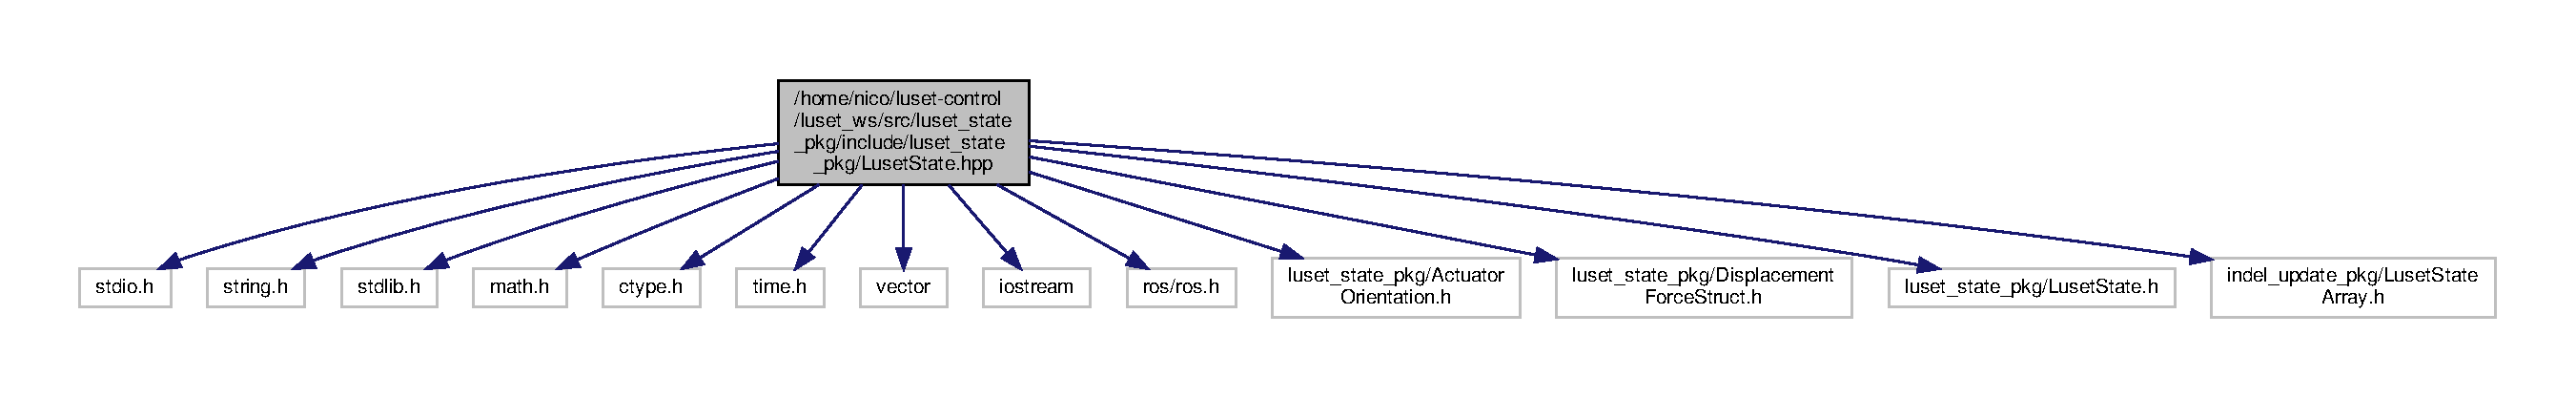
\includegraphics[width=350pt]{LusetState_8hpp__incl}
\end{center}
\end{figure}
This graph shows which files directly or indirectly include this file\+:\nopagebreak
\begin{figure}[H]
\begin{center}
\leavevmode
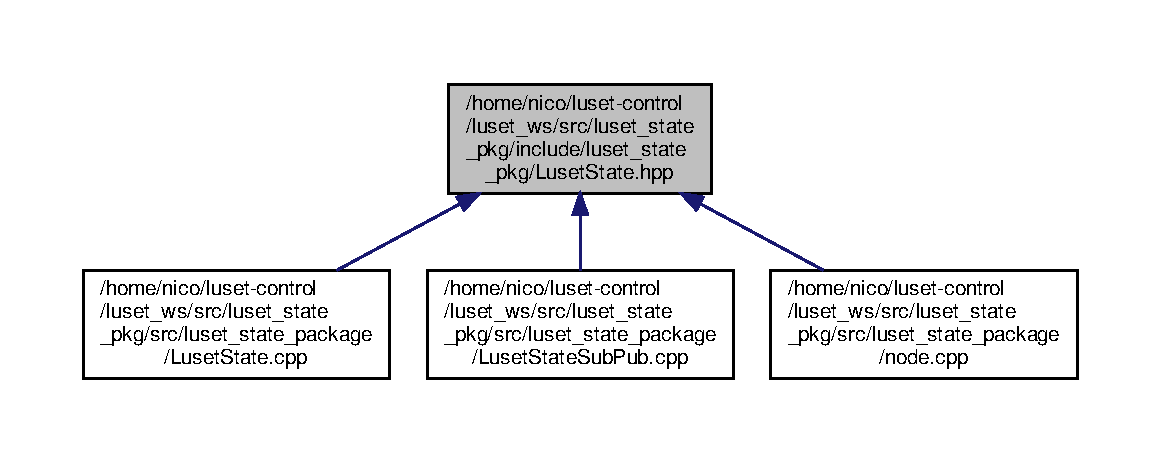
\includegraphics[width=350pt]{LusetState_8hpp__dep__incl}
\end{center}
\end{figure}
\subsection*{Classes}
\begin{DoxyCompactItemize}
\item 
class \hyperlink{classlusetstatenamespace_1_1LusetState}{lusetstatenamespace\+::\+Luset\+State}
\begin{DoxyCompactList}\small\item\em This class parses the Luset\+State\+Array obtained by subscribing to the /\+Indel\+Update topic and publishes a message structure containing all the sensor data acquired from the low-\/level controller. \end{DoxyCompactList}\item 
struct \hyperlink{structlusetstatenamespace_1_1LusetState_1_1DisplacementForce}{lusetstatenamespace\+::\+Luset\+State\+::\+Displacement\+Force}
\item 
class \hyperlink{classlusetstatepubsubnamespace_1_1LusetStatePubSub}{lusetstatepubsubnamespace\+::\+Luset\+State\+Pub\+Sub}
\end{DoxyCompactItemize}
\subsection*{Namespaces}
\begin{DoxyCompactItemize}
\item 
 \hyperlink{namespacelusetstatenamespace}{lusetstatenamespace}
\begin{DoxyCompactList}\small\item\em $<$ For access to R\+O\+S-\/specific functions \end{DoxyCompactList}\item 
 \hyperlink{namespacelusetstatepubsubnamespace}{lusetstatepubsubnamespace}
\end{DoxyCompactItemize}


\subsection{Detailed Description}
This is the header file for the Luset\+State and Luset\+State\+Pub classes. See \href{https://google.github.io/styleguide/cppguide.html}{\tt https\+://google.\+github.\+io/styleguide/cppguide.\+html} for Google Style Guide for C++. 

\begin{DoxyAuthor}{Author}
Nicholas José Palomo (\href{mailto:npalomo@student.ethz.ch}{\tt npalomo@student.\+ethz.\+ch}) 
\end{DoxyAuthor}
\begin{DoxyVersion}{Version}
0.\+1 
\end{DoxyVersion}
\begin{DoxyDate}{Date}
2020-\/02-\/24
\end{DoxyDate}
\begin{DoxyCopyright}{Copyright}
Copyright (c) 2020 
\end{DoxyCopyright}

\hypertarget{LusetState_8cpp}{}\section{/home/nico/luset-\/control/luset\+\_\+ws/src/luset\+\_\+state\+\_\+pkg/src/luset\+\_\+state\+\_\+package/\+Luset\+State.cpp File Reference}
\label{LusetState_8cpp}\index{/home/nico/luset-\/control/luset\+\_\+ws/src/luset\+\_\+state\+\_\+pkg/src/luset\+\_\+state\+\_\+package/\+Luset\+State.\+cpp@{/home/nico/luset-\/control/luset\+\_\+ws/src/luset\+\_\+state\+\_\+pkg/src/luset\+\_\+state\+\_\+package/\+Luset\+State.\+cpp}}


This is the source code for the Luset\+State class. See \href{https://google.github.io/styleguide/cppguide.html}{\tt https\+://google.\+github.\+io/styleguide/cppguide.\+html} for Google Style Guide for C++.  


{\ttfamily \#include \char`\"{}Luset\+State.\+hpp\char`\"{}}\newline
Include dependency graph for Luset\+State.\+cpp\+:\nopagebreak
\begin{figure}[H]
\begin{center}
\leavevmode
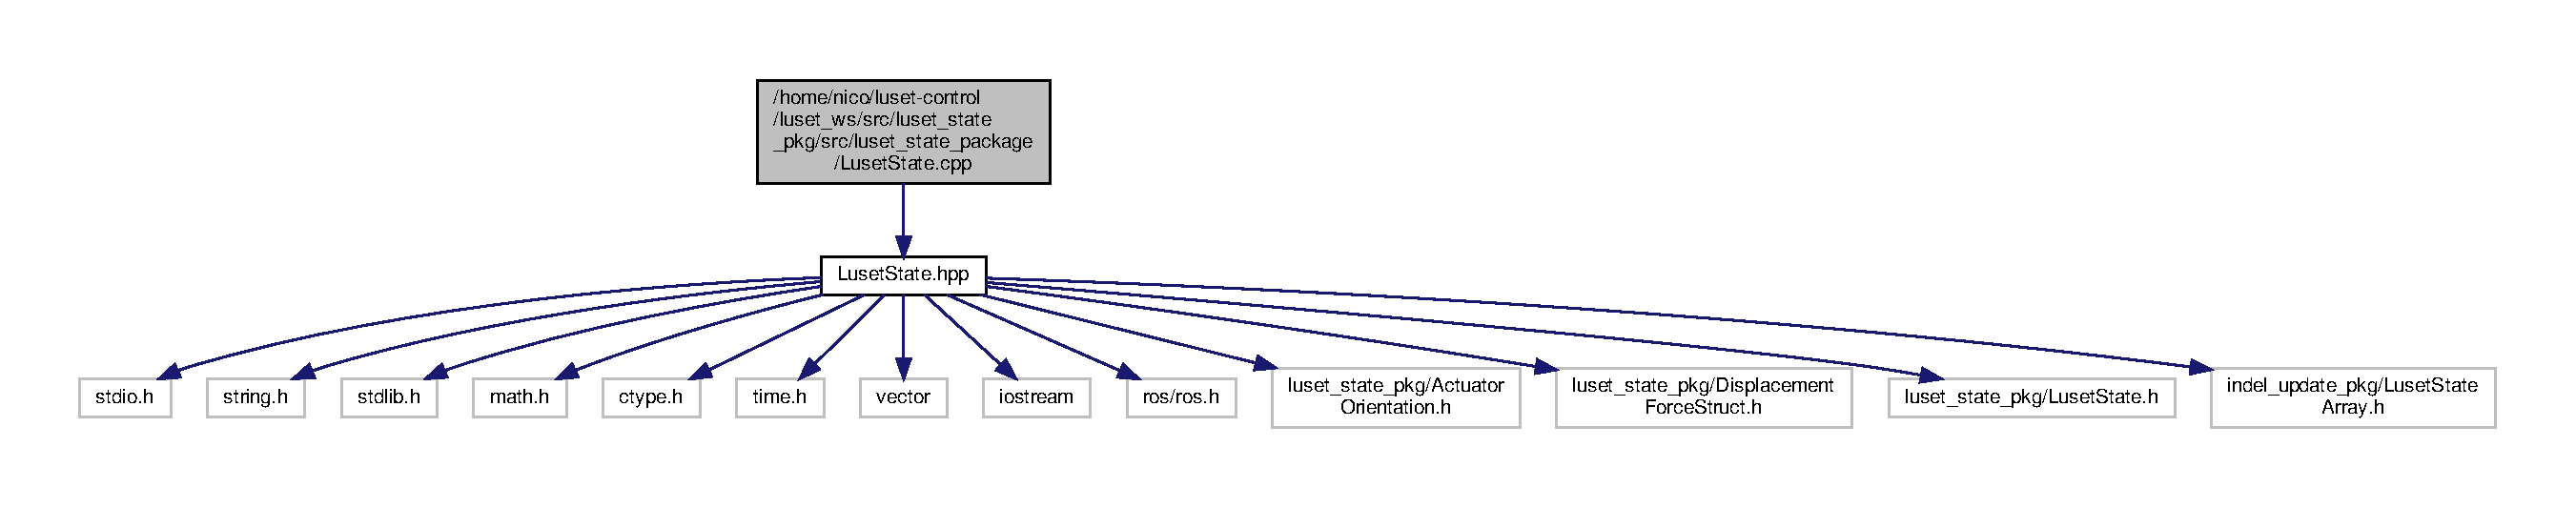
\includegraphics[width=350pt]{LusetState_8cpp__incl}
\end{center}
\end{figure}


\subsection{Detailed Description}
This is the source code for the Luset\+State class. See \href{https://google.github.io/styleguide/cppguide.html}{\tt https\+://google.\+github.\+io/styleguide/cppguide.\+html} for Google Style Guide for C++. 

\begin{DoxyAuthor}{Author}
Nicholas José Palomo (\href{mailto:npalomo@student.ethz.ch}{\tt npalomo@student.\+ethz.\+ch}) 
\end{DoxyAuthor}
\begin{DoxyVersion}{Version}
0.\+1 
\end{DoxyVersion}
\begin{DoxyDate}{Date}
2020-\/02-\/24
\end{DoxyDate}
\begin{DoxyCopyright}{Copyright}
Copyright (c) 2020 
\end{DoxyCopyright}

\hypertarget{LusetStateSubPub_8cpp}{}\section{/home/nico/luset-\/control/luset\+\_\+ws/src/luset\+\_\+state\+\_\+pkg/src/luset\+\_\+state\+\_\+package/\+Luset\+State\+Sub\+Pub.cpp File Reference}
\label{LusetStateSubPub_8cpp}\index{/home/nico/luset-\/control/luset\+\_\+ws/src/luset\+\_\+state\+\_\+pkg/src/luset\+\_\+state\+\_\+package/\+Luset\+State\+Sub\+Pub.\+cpp@{/home/nico/luset-\/control/luset\+\_\+ws/src/luset\+\_\+state\+\_\+pkg/src/luset\+\_\+state\+\_\+package/\+Luset\+State\+Sub\+Pub.\+cpp}}


This is the source code for the subscriber/publisher/callback Luset\+State\+Sub\+Pub class. See \href{https://google.github.io/styleguide/cppguide.html}{\tt https\+://google.\+github.\+io/styleguide/cppguide.\+html} for Google Style Guide for C++.  


{\ttfamily \#include \char`\"{}Luset\+State.\+hpp\char`\"{}}\newline
Include dependency graph for Luset\+State\+Sub\+Pub.\+cpp\+:\nopagebreak
\begin{figure}[H]
\begin{center}
\leavevmode
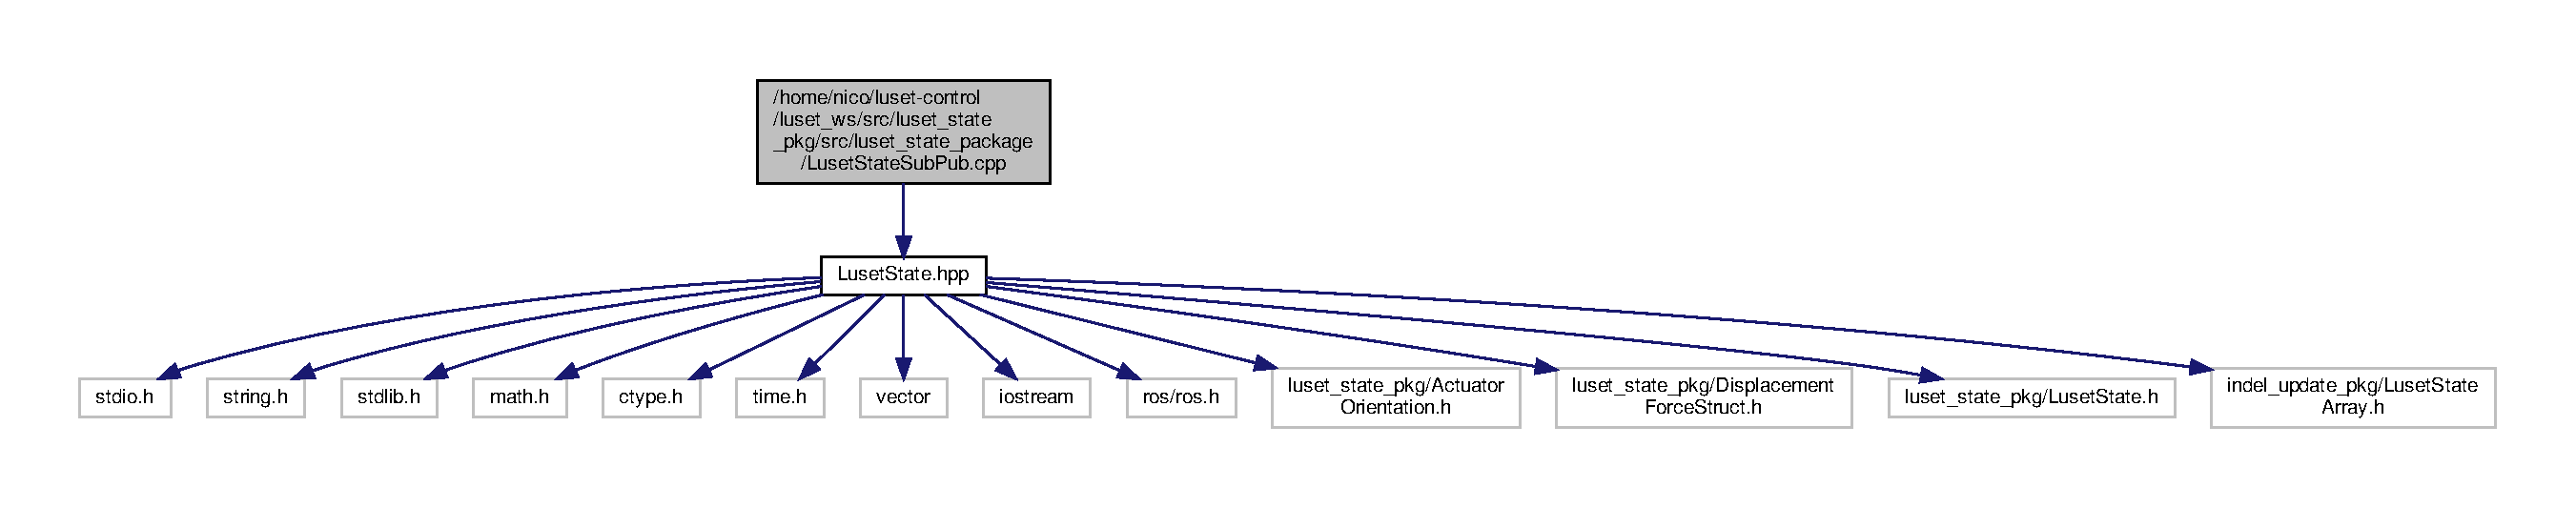
\includegraphics[width=350pt]{LusetStateSubPub_8cpp__incl}
\end{center}
\end{figure}


\subsection{Detailed Description}
This is the source code for the subscriber/publisher/callback Luset\+State\+Sub\+Pub class. See \href{https://google.github.io/styleguide/cppguide.html}{\tt https\+://google.\+github.\+io/styleguide/cppguide.\+html} for Google Style Guide for C++. 

\begin{DoxyAuthor}{Author}
Nicholas José Palomo (\href{mailto:npalomo@student.ethz.ch}{\tt npalomo@student.\+ethz.\+ch}) 
\end{DoxyAuthor}
\begin{DoxyVersion}{Version}
0.\+1 
\end{DoxyVersion}
\begin{DoxyDate}{Date}
2020-\/02-\/24
\end{DoxyDate}
\begin{DoxyCopyright}{Copyright}
Copyright (c) 2020 
\end{DoxyCopyright}

%--- End generated contents ---

% Index
\backmatter
\newpage
\phantomsection
\clearemptydoublepage
\addcontentsline{toc}{chapter}{Index}
\printindex

\end{document}
